\documentclass[oneside]{book} % consider draft option

\usepackage{scrextend}
\usepackage{xparse}
\usepackage{nth}
\usepackage{mathptmx}
\usepackage{enumitem}
\usepackage{comment}    %Provides comments
\usepackage{array}    %Provides \arraybackslash
\usepackage{tabularx}    %Provides almost all of the tables
\usepackage[dvipsnames,svgnames,usenames,table]{xcolor}    %Colors the tables
%Set table captions to appear on the left side of the table
\usepackage[font=bf,justification=raggedright,singlelinecheck=off]{caption}
%Use more compact section headers
\usepackage[compact]{titlesec}
\usepackage{fancyhdr}
\usepackage{longtable}
\usepackage{tabu}
\usepackage{booktabs}
\usepackage{xspace}
\usepackage{changepage}
\usepackage{makecell}

%\usepackage{placeins} This made layout screwy
\usepackage{multicol}

% function math stuff
\usepackage{tikz}
% borders
\usepackage[framemethod=tikz]{mdframed}

% variable width columns
%\usepackage{vwcol}

%Makes text look better
\usepackage{microtype}

\usepackage{siunitx}

\usepackage{xstring}
\usepackage{gensymb}
\usepackage{ragged2e}

\usepackage[pdftex,bookmarks=true,breaklinks=true,colorlinks=true,linkcolor=MidnightBlue,bookmarksopen=true,bookmarksopenlevel=1,bookmarksdepth=1]{hyperref}
% \usepackage[tex4ht,bookmarks=true,breaklinks=true,colorlinks=true,linkcolor=MidnightBlue,bookmarksopen=true,bookmarksopenlevel=1,bookmarksdepth=1]{hyperref}

\newcommand{\lcaption}[1]{\caption{#1}\label{cap:#1}}

\newcommand{\pref}[1]{page \pageref{#1}}
\newcommand{\tref}[1]{Table \ref{cap:#1}: #1 (\pref{cap:#1})}
\newcommand{\trefnp}[1]{Table \ref{cap:#1}: #1}

\newcommand{\minus}{\texttt{-{}}}
\newcommand{\plus}{\texttt{+}}    %Use a smaller positive marker for use directly adjacent to numbers
\newcommand{\add}{\texttt{+}\xspace}    %Use a smaller plus sign
\newcommand{\sub}{\texttt{-}\xspace}
\newcommand{\mult}{x}
\newcommand{\x}{x\xspace}
%NOTED BUG: Spell names with mixed capitalization (Dispel magic) will not work properly.
\newcommand{\combatstyle}[1]{\emph{\mbox{\hyperlink{style:#1}{#1}}}}    %Italicize combat styles
\newcommand{\sphere}[1]{\emph{\mbox{\hyperlink{spell:#1}{#1}}}}    %Italicize mystic spheres
\newcommand{\ability}[1]{\emph{\mbox{\hyperlink{ability:#1}{#1}}}}    %Italicize mystic spheres
\newcommand{\spell}[1]{\emph{\mbox{\hyperlink{spell:#1}{#1}}}}    %Italicize spells
\newcommand{\maneuver}[1]{\emph{\mbox{\hyperlink{maneuver:#1}{#1}}}}    %Italicize maneuvers
\newcommand{\stance}[1]{\emph{\mbox{\hyperlink{stance:#1}{#1}}}}    %Italicize maneuvers
\newcommand{\spellindirect}[2]{\emph{\hyperlink{spell:#1}{#2}}}
\newcommand{\ritual}[1]{\emph{#1}}    %Italicize spells
\newcommand{\subcf}[1]{\parhead{#1}}    %Bold sub-class-feature headers
\newcommand{\subsk}[1]{\par \emph{#1}:}    %Italicize sub-skill headers

\newcommand{\subparhead}[1]{\par\emph{#1}:}
\newcommand{\tb}[1]{\textbf{#1}}    %Bold the header of tables
\newcommand{\tdash}{\hskip 0.1em---\xspace}    %A null entry in a table
\newcommand{\ccol}{\centering\arraybackslash}    %Center columns
\newcommand{\lcol}{\raggedright\arraybackslash}
\newcommand{\rcol}{\raggedleft\arraybackslash}

\newcommand{\fn}[1]{\textsuperscript{#1}}
\newcommand{\magicitem}[1]{\emph{#1}}    %For the names of items
\newcommand{\mitem}[1]{\emph{#1}}

\newcommand{\tind}{\hspace{1em}}

\newcommand{\spelldesc}[1]{\par\noindent \textit{#1}}
\newcommand{\spelltwocol}[2]{\spelltabularcompressed #1 & #2\end{tabularx}}

\newcommand{\rngshort}{Short \reminder{30 ft.}\xspace}
\newcommand{\rngmed}{Medium \reminder{60 ft.}\xspace}
\newcommand{\rnglong}{Long \reminder{120 ft.}\xspace}
\newcommand{\rngdist}{Distant \reminder{240 ft.}\xspace}
\newcommand{\rngext}{Extreme \reminder{480 ft.}\xspace}

\newcommand{\shortrange}{Short \reminder{30 ft.} range\xspace}
\newcommand{\medrange}{Medium \reminder{60 ft.} range\xspace}
\newcommand{\longrange}{Long \reminder{120 ft.} range\xspace}
\newcommand{\distrange}{Distant \reminder{240 ft.} range\xspace}
\newcommand{\extrange}{Extreme \reminder{480 ft.} range\xspace}

\newcommand{\areatiny}{Tiny \reminder{5 ft.}\xspace}
\newcommand{\areasmall}{Small \reminder{15 ft.}\xspace}
\newcommand{\areamed}{Medium \reminder{30 ft.}\xspace}
\newcommand{\arealarge}{Large \reminder{60 ft.}\xspace}
\newcommand{\areahuge}{Huge \reminder{120 ft.}\xspace}
\newcommand{\areagarg}{Gargantuan \reminder{240 ft.}\xspace}

\newcommand{\tinyarea}{Tiny \reminder{5 ft.}\xspace}
\newcommand{\smallarea}{Small \reminder{15 ft.}\xspace}
\newcommand{\medarea}{Medium \reminder{30 ft.}\xspace}
\newcommand{\largearea}{Large \reminder{60 ft.}\xspace}
\newcommand{\hugearea}{Huge \reminder{120 ft.}\xspace}
\newcommand{\gargarea}{Gargantuan \reminder{240 ft.}\xspace}

\newcommand{\tinyarealong}{Tiny \reminder{5 ft. long}\xspace}
\newcommand{\smallarealong}{Small \reminder{15 ft. long}\xspace}
\newcommand{\medarealong}{Medium \reminder{30 ft. long}\xspace}
\newcommand{\largearealong}{Large \reminder{60 ft. long}\xspace}
\newcommand{\hugearealong}{Huge \reminder{120 ft. long}\xspace}
\newcommand{\gargarealong}{Gargantuan \reminder{240 ft. long}\xspace}

\newcommand{\confusionexplanation}{A confused creature cannot take actions normally. If it is attacked, it automatically attacks a random attacker. Otherwise, at the beginning of each round, it randomly decides to take one of four actions that round: babble incoherently, flee from the caster as if panicked, attack the nearest creature, or act normally. A confused character who can't carry out the indicated action does nothing but babble incoherently.\xspace}

\newcommand{\featpre}{\parhead{Prerequisite} }
\newcommand{\featpres}{\parhead{Prerequisites} }
%featref no target
\newcommand{\featpref}[1]{\pageref{feat:#1}}
\newcommand{\mitempref}[1]{\pageref{item:#1}}
\newcommand{\featpcref}[1]{#1, page \pageref{feat:#1}}

\newcommand{\skill}[2]{\section{#1 (#2)}\label{#1}}

\newcommand{\reminder}[1]{\textcolor{darkgray}{\textit{(#1)}}}

%\newcommand{\vulnerableexplanation}{A vulnerable creature takes a \minus2 penalty to attacks, defenses, and checks.\xspace}
%\newcommand{\vulneffect}{\minus2 to attacks, defenses, and checks\xspace}

\newcommand{\blinded}{\debuff{blinded} \reminder{50\% miss chance}\xspace}
\newcommand{\charmed}{\debuff{charmed} \reminder{friendly with charmer}\xspace}
\newcommand{\confused}{\debuff{confused} \reminder{acts randomly}\xspace}
\newcommand{\dazed}{\debuff{dazed} \reminder{\minus2 defenses}\xspace}
\newcommand{\dazzled}{\debuff{dazzled} \reminder{\minus2 accuracy, no special vision}\xspace}
\newcommand{\deafened}{\debuff{deafened} \reminder{20\% verbal spell failure}\xspace}
\newcommand{\decelerated}{\debuff{decelerated} \reminder{\minus4 Armor and Ref, delayed actions}\xspace}
\newcommand{\disoriented}{\debuff{disoriented} \reminder{moves in random directions}\xspace}
\newcommand{\dominated}{\debuff{dominated} \reminder{must obey commands}\xspace}
\newcommand{\fascinated}{\debuff{fascinated} \reminder{cannot act, \minus5 to observe anything}\xspace}
\newcommand{\frightened}{\debuff{frightened} \reminder{\minus4 accuracy and Mental within 60 ft.}\xspace}
% Too complicated to try to summarize :/
\newcommand{\grappled}{\debuff{grappled}\xspace}
\newcommand{\helpless}{\debuff{helpless} \reminder{\minus10 or more Armor and Ref}\xspace}
\newcommand{\immobilized}{\debuff{immobilized} \reminder{cannot use movement speeds}\xspace}
\newcommand{\nauseated}{\debuff{nauseated} \reminder{\minus4 all defenses}\xspace}
\newcommand{\panicked}{\debuff{panicked} \reminder{\minus4 Mental and must flee within 60 ft.}\xspace}
\newcommand{\paralyzed}{\debuff{paralyzed} \reminder{cannot move}\xspace}
\newcommand{\partiallyunaware}{\debuff{partially unaware} \reminder{\minus2 Armor and Ref}\xspace}
\newcommand{\petrified}{\debuff{petrified}\xspace}
\newcommand{\prone}{\debuff{prone} \reminder{quarter speed, \minus2 strike accuracy, Armor, and Ref}\xspace}
\newcommand{\shaken}{\debuff{shaken} \reminder{\minus2 accuracy and Mental within 60 ft.}\xspace}
\newcommand{\sickened}{\debuff{sickened} \reminder{\minus2 all defenses}\xspace}
\newcommand{\slowed}{\debuff{slowed} \reminder{half speed, \minus2 Armor and Ref}\xspace}
\newcommand{\squeezing}{\debuff{squeezing} \reminder{\minus2 accuracy, Armor, and Ref}\xspace}
\newcommand{\stunned}{\debuff{stunned} \reminder{\minus4 all defenses}\xspace}
\newcommand{\surrounded}{\debuff{surrounded} \reminder{\minus2 Armor and Ref}\xspace}
\newcommand{\unaware}{\debuff{unaware} \reminder{\minus5 Armor and Ref}\xspace}
\newcommand{\unconscious}{\debuff{unconscious}\xspace}

\newcommand{\spelltablecolumns}{>{\lcol}X l}
\newcommand{\spelllevelschool}[2]{\spelllvl{#1} & #2 \\}
\newcommand{\spelllevelnew}[3]{\tb{\nth{#1} level} #2 & #3 \\}

\newcommand{\dismissable}{}

\ExplSyntaxOn

\DeclareDocumentCommand{\parhead}{s m o}
{
    \par
    \IfNoValueTF{#3}
    {\textbf{#2}:}
    {\textbf{#2}~[#3]:}\xspace
}

\DeclareDocumentCommand{\parheadindent}{s m o}
{
    \par
    \IfNoValueTF{#3}
    {\textbf{#2}:}
    {\textbf{#2}~[#3]:}\xspace
}

\DeclareDocumentCommand{\rank}{m}
{
    \par \noindent
    Rank~#1:\xspace
}

\DeclareDocumentCommand{\featlevel}{m}
{
    \par \noindent
    \textit{Level~#1}:
}

\DeclareDocumentCommand{\rankline}{}
{
    \par
    \vspace{-0.5em}
    \noindent
    \hrulefill
    \par\noindent
}

% If #1 = #2
%     print #3.
% Elseif #4 is provided
%     print #4
\DeclareDocumentCommand{\ifstr}{m m m o}
{
    \ifnum 0=\pdfstrcmp{#1}{#2}
        #3
    \else
        \IfValueT{#4}{#4}
    \fi
}

% args:
%   pre-spell header spell name, spell name modifier (Greater, etc.)
\DeclareDocumentCommand{\spellhead}{o m o}
{
    \IfValueTF{#1}
    {\item[#1]}
    {\item}
    \textbf{
        \IfValueTF{#3}
        {
            \hyperlink{spell:#3~#2}{#2,~#3}
            %\pageref{spell:#3~#2}
        }
        {
            \hyperlink{spell:#2}{#2}
            %\pageref{spell:#2}
        }
    }:
}

% args:
%   pre-spell header spell name, spell name modifier (Greater, etc.)
\DeclareDocumentCommand{\maneuverhead}{o m o}
{
    \IfValueTF{#1}
    {\item[#1]}
    {\item}
    \textbf{
        \IfValueTF{#3}
        {
            \hyperlink{maneuver:#3~#2}{#2,~#3}
            \hypertarget{maneuverlist:#3~#2}
        }
        {
            \hyperlink{maneuver:#2}{#2}
            \hypertarget{maneuverlist:#2}
        }
    }:
}

\DeclareDocumentCommand{\imath}{m}
{
    %\pgfmathparse{int(floor(#1))}\pgfmathresult
    \pgfmathsetmacro{\TempVar}{int(floor(#1))}
    \TempVar
}

\DeclareDocumentCommand{\imathparse}{m}
{
    \pgfmathsetmacro{\TempVar}{int(floor(#1))}
}

\DeclareDocumentCommand{\imathresult}{}
{
    \TempVar
}

\DeclareDocumentCommand{\spelltabular}{}
{
    \par\noindent
    \begin{tabularx}{\columnwidth}{>{\lcol}X l}
}

\DeclareDocumentCommand{\spelltabularcompressed}{}
{
    \renewcommand{\arraystretch}{0.5}
    \par\noindent
    \begin{tabularx}{\linewidth}{@{}~>{\lcol}X~l~@{}}
}

% args:
%   class name
%   level, if any
%   ability name
%   ability type (Ex, Su, etc.), if any
\DeclareDocumentCommand{\cf}{s m o m o}
{
    \IfValueTF{#3}
    {
        \IfValueTF{#5}
        { \subsubsection{Rank~#3~--~#4~(#5)} }
        { \subsubsection{Rank~#3~--~#4} }
    }
    {
        \IfValueTF{#5}
        { \subsubsection{#4~(#5)} }
        { \subsubsection{#4} }
    }
    \IfBooleanF{#1}
    {
        \label{#2:#4}
    }
}

% feat level
% args:
%   level
%   name
%   ability type, if any
\DeclareDocumentCommand{\ff}{o m o}
{
    \IfValueTF{#1}
    {
        \IfValueTF{#3}
        { \nth{#1}~--~\textbf{#2}~(#3): }
        { \nth{#1}~--~\textbf{#2}: }
    }
    {
        \IfValueTF{#3}
        { \parhead{#2~(#3)} }
        { \parhead{#2} }
    }
}

\DeclareDocumentCommand{\itemhead}{s m}
{
    \item
    \IfValueTF{#1}
    {
        \textit{#2}
    }
    {
        \textbf{#2}
    }
}

\DeclareDocumentCommand{\featref}{s m}
{
    \hyperlink{feat:#2}{#2}
    \IfBooleanF{#1}
    {
        \hypertarget{ft:#2}{}
    }
}

% args:
%   #1: reference name of term, if different from display name
%   #2: display name of term
%   #3: hyperlink prefix
\DeclareDocumentCommand{\termlink}{o m m}
{
    \IfValueTF{#1}
    {
        % Enable this to test for missing glossary definitions
        % \pref{#1}
        % Enable this to test for unnecessary glossary entries
        % \label{#1}

        % TODO: remove \mbox before making major releases;
        % it fixes bizarre page break errors but makes text uglier
        \hyperlink{#3:#1}{\textbf{\mbox{#2}}}
    }
    {
        % Enable this to test for missing glossary definitions
        % \pref{#2}
        % Enable this to test for unnecessary glossary entries
        % \label{#2}

        \hyperlink{#3:#2}{\textbf{\mbox{#2}}}
    }
}

% args:
%   #1: name of term
%   #2: alternate name of term, only used for labels/targets
%   #3: hyperlink prefix
\DeclareDocumentCommand{\termdef}{m o m}
{
    \IfValueT{#2}
    {
        % Enable this to test for missing glossary definitions
        % \label{#2}\label{#2s}
        % Enable this to test for unnecessary glossary entries
        % \pref{#2}

        \hypertarget{#3:#2}{}
        \hypertarget{#3:#2s}{}
    }
    % Enable this to test for missing glossary definitions
    % \label{#1}\label{#1s}
    % Enable this to test for unnecessary glossary entries
    % \pref{#1}

    \hypertarget{#3:#1}{}
    \hypertarget{#3:#1s}{}
    \parhead{#1}
}


\DeclareDocumentCommand{\glossterm}{o m}
{
    \IfValueTF{#1}
    {\termlink[#1]{#2}{gloss}}
    {\termlink{#2}{gloss}}
}
\DeclareDocumentCommand{\glossdef}{m o}
{
    \IfValueTF{#2}
    {\termdef{#1}[#2]{gloss}}
    {\termdef{#1}{gloss}}
}

\DeclareDocumentCommand{\debuff}{o m}
{
    \IfValueTF{#1}
    {\termlink[#1]{#2}{debuff}}
    {\termlink{#2}{debuff}}
}
\DeclareDocumentCommand{\debuffdef}{m o}
{
    \IfValueTF{#2}
    {\termdef{#1}[#2]{debuff}}
    {\termdef{#1}{debuff}}
}


\DeclareDocumentCommand{\abilitytag}{o m}
{
    \IfValueTF{#1}
    {\termlink[#1]{#2}{abilitytag}}
    {\termlink{#2}{abilitytag}}
}
\DeclareDocumentCommand{\abilitytagdef}{m o}
{
    \IfValueTF{#2}
    {\termdef{#1}[#2]{abilitytag}}
    {\termdef{#1}{abilitytag}}
}

\DeclareDocumentCommand{\pcref}{o m}
{
    \IfValueTF{#1}
    {
        #2,~page~\pageref{#1}
    }
    {
        #2,~page~\pageref{#2}
    }
}

\DeclareDocumentCommand{\hit}{}
{
    \par \textbf{Hit}:\xspace
}

\DeclareDocumentCommand{\glance}{}
{
    \par \textbf{Glancing~blow}:\xspace
}


\DeclareDocumentCommand{\crit}{}
{
    \par \textbf{Critical~hit}:\xspace
}

\DeclareDocumentCommand{\miss}{}
{
    \par \textbf{Miss}:\xspace
}

\DeclareDocumentCommand{\tableheaderrule}{}
{
    \vspace{-0.25em}
    \\
    \bottomrule
}

\DeclareDocumentCommand{\targetrule}{s}{
    \par
    \vspace{-0.5em}
    \noindent
    \hrulefill
    \par\noindent
}

\DeclareDocumentCommand{\target}{m}{
    \par\noindent
    Target:~#1
    \targetrule*
}

\DeclareDocumentCommand{\targets}{m}{
    \par\noindent
    Targets:~#1
    \targetrule
}

\DeclareDocumentCommand{\monsep}{}{
    \hspace{0.8em}
}

\ExplSyntaxOff

\newcommand{\classbasics}[1]{\par\noindent\textbf{#1}:}

\newcommand{\pari}{\par\noindent}

%Set the spacing of lists
\newenvironment{enumerate*}
{\begin{enumerate}
  \setlength{\leftmargin}{0em}
  \setlength{\topsep}{1pt}
  \setlength{\itemsep}{1pt}
  \setlength{\parskip}{0pt}
  \setlength{\parsep}{0pt}}
{\end{enumerate}}

%Define a custom table that uses that coloring
\newenvironment{dtable}
{\begin{table}[htb!]
  \small
  \rowcolors{1}{white}{tbrown}}
{\end{table}}
%Plus a custom table that takes up two columns
\newenvironment{dtable*}
{\begin{table*}[htb!]
  \small
  \rowcolors{1}{white}{tbrown}}
{\end{table*}}
%And one more for two-column tables that need fewer restrictions
\newenvironment{dtable!*}
{\begin{table*}[htb!]
    \small
    \rowcolors{1}{white}{tbrown}
}{
    \end{table*}
}

% small text for the feats table
\newenvironment{longtablewrapper}
{
    \onecolumn
    \small
    \rowcolors{1}{white}{tbrown}
    \renewcommand*{\arraystretch}{1.2}
    \setlength\LTleft{0pt}
    \setlength\LTright{0pt}
}
{\twocolumn}

%A list for normal spells
\newenvironment{spelllist}
{\begin{description}[nosep,font=\normalfont,leftmargin=2.25em,style=nextline,itemindent=-1em]}
{\end{description}}

\ExplSyntaxOn

\DeclareDocumentEnvironment{fakehang}{}
{
    \setlength{\parindent}{2em}
    \everypar{\hangindent=1em}
}
{
    \par
}

\DeclareDocumentEnvironment{spellheader}{s}
{
    %\IfBooleanF{#1}{\spellline}
}
{
    %\IfBooleanF{#1}{\spellline}
}

\DeclareDocumentEnvironment{spellcontent}{}
{
    \begin{thesamepage}
}
{
    \end{thesamepage}
}
\surroundwithmdframed[
    style=spellcontent,
    leftline=true,
    topline=true,
    rightline=true,
    bottomline=true,
]{spellcontent}

\definecolor{cosmiclatte}{rgb}{1.0, 0.97, 0.91}

\DeclareDocumentEnvironment{freeability}{o m o}
{
    \begin{thesamepage}
    \RaggedRight
    \lowercase{\hypertarget{ability:#2}{}}
    \hypertarget{ability:#2}{}
    \spelltwocol{
        {\normalsize \textbf{#2}}
        \IfValueTF{#1}{~--~#1}{}
    }{
        \IfValueTF{#3}{#3}{}
    }
}
{
    \end{thesamepage}
}
\surroundwithmdframed[
    backgroundcolor=cosmiclatte,
    leftline=true,
    topline=true,
    rightline=true,
    bottomline=true,
    roundcorner=4pt,
    skipabove=0.25em,
    skipbelow=0.5em,
    innerleftmargin=0.25em,
    innerrightmargin=0.5em,
    innertopmargin=-0.1em,  % using thesamepage gives it a top margin
    innerbottommargin=0.25em,
]{freeability}

\DeclareDocumentEnvironment{durationability}{o m o}
{
    \begin{thesamepage}
    \RaggedRight
    \lowercase{\hypertarget{ability:#2}{}}
    \hypertarget{ability:#2}{}
    \spelltwocol{
        {\normalsize \textbf{#2}}
        \IfValueTF{#1}{~--~#1}{}
    }{
        \IfValueTF{#3}{#3}{}
    }
}
{
    \end{thesamepage}
}
\surroundwithmdframed[
    backgroundcolor=cosmiclatte,
    leftline=true,
    topline=true,
    rightline=true,
    bottomline=true,
    roundcorner=4pt,
    skipabove=0.25em,
    skipbelow=0.5em,
    innerleftmargin=0.25em,
    innerrightmargin=0.5em,
    innertopmargin=-0.1em,  % using thesamepage gives it a top margin
    innerbottommargin=0.25em,
]{durationability}

\DeclareDocumentEnvironment{attuneability}{o m o}
{
    \begin{thesamepage}
    \RaggedRight
        \lowercase{\hypertarget{ability:#2}{}}
        \hypertarget{ability:#2}{}
        \spelltwocol{
            {\normalsize \textbf{#2}}
            \IfValueTF{#1}{~--~#1}{}
        }{#3}
}
{
    \end{thesamepage}
}
\surroundwithmdframed[
    backgroundcolor=brown!8,
    leftline=true,
    topline=true,
    rightline=true,
    bottomline=true,
    roundcorner=4pt,
    skipabove=0.25em,
    skipbelow=0.5em,
    innerleftmargin=0.25em,
    innerrightmargin=0.5em,
    innertopmargin=-0.1em,  % using thesamepage gives it a top margin
    innerbottommargin=0.25em,
]{attuneability}

\DeclareDocumentEnvironment{instantability}{o m o}
{
    \begin{thesamepage}
    \RaggedRight
    \lowercase{\hypertarget{ability:#2}{}}
    \hypertarget{ability:#2}{}
    \spelltwocol{
        {\normalsize \textbf{#2}}
        \IfValueTF{#1}{~--~#1}{}
    }{
        \IfValueTF{#3}{#3}{}
    }
}
{
    \end{thesamepage}
}
\surroundwithmdframed[
    backgroundcolor=MintCream,
    leftline=true,
    topline=true,
    rightline=true,
    bottomline=true,
    roundcorner=4pt,
    skipabove=0.25em,
    skipbelow=0.5em,
    innerleftmargin=0.25em,
    innerrightmargin=0.5em,
    innertopmargin=-0.1em,  % using thesamepage gives it a top margin
    innerbottommargin=0.25em,
]{instantability}

\newmdenv[
    style=colorenv,
    backgroundcolor=LightCyan,
]{spelltargetinginfo}

\newmdenv[
    style=colorenv,
    backgroundcolor=LightCyan,
]{augmenttargetinginfo}

\DeclareDocumentEnvironment{spelleffects}{}
{}
{}
\surroundwithmdframed[
    style=colorenv,
    backgroundcolor=Lavender,
]{spelleffects}

\DeclareDocumentEnvironment{augmenteffects}{}
{}
{}
\surroundwithmdframed[
    style=colorenv,
    backgroundcolor=Lavender,
]{augmenteffects}

\DeclareDocumentEnvironment{spellfooter}{}
{}
{}
\surroundwithmdframed[
    style=colorenv,
    backgroundcolor=Gainsboro,
    leftline=true,
    rightline=true,
]{spellfooter}

\DeclareDocumentEnvironment{monsterfooter}{}
{
    \begin{fakehang}
}
{
    \end{fakehang}
}
\surroundwithmdframed[
    style=colorenv,
    backgroundcolor=Gainsboro,
    leftline=true,
    rightline=true,
    bottomline=true,
]{monsterfooter}

\DeclareDocumentEnvironment{dtabularx}{m m}
{
    \tabularx{#1}{#2}%
}
{
    \endtabularx
}

\surroundwithmdframed{dtabularx}

\DeclareDocumentEnvironment{spellsection}{o m o}
{
    \begin{thesamepage}
    \setlength{\multicolsep}{0pt}
    \begin{multicols}{2}
        \IfValueTF{#1}
        {
            \lowercase{\hypertarget{spell:#1~#2}{}}\label{spell:#1~#2}
            \hypertarget{spell:#1~#2}
                {\subsubsection{#2,~#1}}
        }
        {
            \lowercase{\hypertarget{spell:#2}{}}\label{spell:#2}
            \hypertarget{spell:#2}
                {\subsection{#2}}
        }
        \IfValueTF{#3}
        {
            \columnbreak
            \begin{flushright}
                \large\textbf{\nth{#3}~Level}
            \end{flushright}
        }
        {
            \columnbreak
            \begin{flushright}
            \end{flushright}
        }
    \end{multicols}
}
{
    \end{thesamepage}
}

\DeclareDocumentEnvironment{thesamepage}{}
{
    \par\nobreak\vfil\penalty0\vfilneg
    \vtop{}
}
{
    \par\xdef\tpd{\the\prevdepth}
    \prevdepth=\tpd
}

\DeclareDocumentEnvironment{feat}{m m}
{
    \subsection*{
        \hypertarget{feat:#1}{
            \hyperlink{ft:#1}{#1~[#2]}
        }
    }
    \label{feat:#1}
}
{}

\DeclareDocumentEnvironment{monsection}{m o m o}
{
    \vspace{1em}
    \begin{thesamepage}
    \setlength\multicolsep{0pt}
    \begin{multicols}{2}
        \IfValueTF{#2}
        {
            \lowercase{\hypertarget{mon:#2~#1}{}}
            \label{mon:#2~#1}
            \hypertarget{mon:#2~#1}
                {\subsection{#1,~#2}}
        }
        {
            \lowercase{\hypertarget{mon:#1}{}}
            \label{mon:#1}
            \hypertarget{mon:#1}
                {\subsection{#1}}
        }

        \columnbreak
        \begin{flushright}
            \large\textbf{Level~#3}
            \IfValueTF{#4}
            {
                \textbf{~[CR~#4]}
            }
            {
                \textbf{~[CR~1]}
            }
        \end{flushright}
    \end{multicols}
}
{
    \end{thesamepage}
}

\DeclareDocumentEnvironment{monsubsection}{m o m o}
{
    \vspace{1em}
    \begin{thesamepage}
    \setlength\multicolsep{0pt}
    \begin{multicols}{2}
        \IfValueTF{#2}
        {
            \lowercase{\hypertarget{mon:#2~#1}{}}
            \label{mon:#2~#1}
            \hypertarget{mon:#2~#1}
                {\subsubsection{#1,~#2}}
        }
        {
            \lowercase{\hypertarget{mon:#1}{}}
            \label{mon:#1}
            \hypertarget{mon:#1}
                {\subsubsection{#1}}
        }

        \columnbreak
        \begin{flushright}
            \textbf{Level~#3}
            \IfValueTF{#4}
            {
                \textbf{~[CR~#4]}
            }
            {
                \textbf{~[CR~1]}
            }
        \end{flushright}
    \end{multicols}
}
{
    \end{thesamepage}
}

\ExplSyntaxOff


%\DisableLigatures[f,i,t]{encoding = *, family = *}

%make bigger section headers
% \titleformat*{\section}{\hspace*{-0.5em}\LARGE\bfseries}
\titleformat{\section}
    {\LARGE\bfseries}   % The style of the section title
    {}                             % a label prefix
    {0pt}                          % How much space exists between the prefix and the title
    {\hspace{-0.5em}}    % A code representing the section
\titleformat{\subsection}
    {\large\bfseries}   % The style of the section title
    {}                             % a label prefix
    {0pt}                          % How much space exists between the prefix and the title
    {\hspace{-0.5em}}    % A code representing the section
\titleformat{\subsubsection}
    {\bfseries}
    {}
    {0pt}
    {\hspace{-0.5em}}

%Format the page margins
\addtolength{\voffset}{-0.8in}
\addtolength{\textheight}{1.5in}
\addtolength{\hoffset}{-0.6in}
\addtolength{\textwidth}{0.8in}
\setlength{\oddsidemargin}{15.5pt}
\setlength{\evensidemargin}{15.5pt}
% widen middle gap width
\setlength{\columnsep}{2em}

%Leave little extra space between tables and the surrounding text
\setlength{\intextsep}{1em}
%Or between paragraphs
\setlength{\parskip}{0pt}
% This looks better, but reveals a lot of extraneous paragraphs that shouldn't exist
% \setlength{\parskip}{0.1em}
%Make sure the table of contents doesn't include every little thing
\setcounter{tocdepth}{2}

\newlength\levelcol
\newlength\spellcol
\newlength\spellcolpoof
\newlength\savecol
\newlength\savecolpoof
\newlength\babcolgood
\newlength\babcolavg
\newlength\babcolpoor
\setlength\levelcol{1.75em}
\setlength\spellcol{1.1em}
\setlength\spellcolpoof{2em}
\setlength\savecol{1.5em}
\setlength\savecolpoof{2em}
\setlength\babcolgood{4em}
\setlength\babcolavg{4em}
\setlength\babcolpoor{4em}

%Create a color for use with tables
\definecolor{tbrown}{RGB}{255,240,200}
% \tabulinesep=1mm

% make lists less poofy
\setlist{noitemsep,topsep=0pt,parsep=0pt,partopsep=0pt}

% setup for border frames
\ExplSyntaxOn
\mdfsetup{
    innerleftmargin=0,
    leftmargin=0,
    innertopmargin=0,
    skipabove=0,
    innerrightmargin=0,
    rightmargin=0,
    innerbottommargin=0,
    skipbelow=0,
}

% for spell content
\mdfdefinestyle{spellcontent}{
    innertopmargin=0,
    innerleftmargin=0,
    innerrightmargin=0,
    skipabove=2pt,
    innerbottommargin=0,
    skipbelow=0,
}

% for color-only environments
\mdfdefinestyle{colorenv}{
    leftline=false,
    topline=false,
    rightline=false,
    bottomline=false,
    innerleftmargin=2pt,
    leftmargin=0,
    innertopmargin=2pt,
    skipabove=0,
    innerrightmargin=2pt,
    rightmargin=0,
    innerbottommargin=2pt,
    skipbelow=0,
}

%Control chapter headers
\renewcommand{\chaptermark}[1]{\markboth{\chaptername \: \thechapter \: - \: #1}{}}
\renewcommand{\sectionmark}[1]{\markright{#1}}

\ExplSyntaxOff

\sisetup{group-minimum-digits = 4,group-separator = {,}}

% fix headheight warning
\setlength{\headheight}{14pt}

\setlength{\RaggedRightParindent}{\parindent}

% This is not part of lib/packages since it is different for PDF and HTML output
\usepackage[tex4ht,bookmarks=true,breaklinks=true,colorlinks=true,linkcolor=MidnightBlue,bookmarksopen=true,bookmarksopenlevel=1,bookmarksdepth=1]{hyperref}

\ExplSyntaxOn

\DeclareDocumentEnvironment{spellcontent}{}{}{}

\newmdenv[
    style=colorenv,
    backgroundcolor=LightCyan,
]{spelltargetinginfomdframed}
\DeclareDocumentEnvironment{spelltargetinginfo}{}
{
    \begin{spelltargetinginfomdframed}
}
{
    \end{spelltargetinginfomdframed}
}

\newmdenv[
    style=colorenv,
    backgroundcolor=LightCyan,
]{augmenttargetinginfomdframed}
\DeclareDocumentEnvironment{augmenttargetinginfo}{}
{
    \begin{augmenttargetinginfomdframed}
}
{
    \end{augmenttargetinginfomdframed}
}

\newmdenv[
    style=colorenv,
    backgroundcolor=Lavender,
]{spelleffectsmdframed}
\DeclareDocumentEnvironment{spelleffects}{}
{
    \begin{spelleffectsmdframed}
}
{
    \end{spelleffectsmdframed}
}

\newmdenv[
    style=colorenv,
    backgroundcolor=Lavender,
]{augmenteffectsmdframed}
\DeclareDocumentEnvironment{augmenteffects}{}
{
    \begin{augmenteffectsmdframed}
}
{
    \end{augmenteffectsmdframed}
}

\newmdenv[
    style=colorenv,
    backgroundcolor=Gainsboro,
    leftline=true,
    rightline=true,
]{spellfootermdframed}
\DeclareDocumentEnvironment{spellfooter}{}
{
    \begin{spellfootermdframed}
}
{
    \end{spellfootermdframed}
}

\newmdenv[
    style=colorenv,
    backgroundcolor=Gainsboro,
    leftline=true,
    rightline=true,
    bottomline=true,
    topline=true,
]{monsterfootermdframed}
\DeclareDocumentEnvironment{monsterfooter}{}
{
    \begin{monsterfootermdframed}
}
{
    \end{monsterfootermdframed}
}


\DeclareDocumentCommand{\spelltwocol}{m m}
{
    \renewcommand{\arraystretch}{0.5}
    \begin{figure}
    \begin{tabularx}{\linewidth}{>{\lcol}X~l}
        #1 & #2
    \end{tabularx}
    \end{figure}
}

% args:
%   #1: reference name of term, if different from display name
%   #2: display name of term
%   #3: hyperlink prefix
\DeclareDocumentCommand{\termlink}{o m m}
{
    \IfValueTF{#1}
    {
        % Enable this to test for missing glossary definitions
        % \pref{#1}
        % Enable this to test for unnecessary glossary entries
        % \label{#1}

        % \mbox causes inconsistent but bizarre "missing space" issues
        % when used in HTML generation, so we omit it from this file
        \hyperlink{#3:#1}{\textbf{#2}}
    }
    {
        % Enable this to test for missing glossary definitions
        % \pref{#2}
        % Enable this to test for unnecessary glossary entries
        % \label{#2}

        \hyperlink{#3:#2}{\textbf{#2}}
    }
}

\ExplSyntaxOff


\setcounter{tocdepth}{1}

\graphicspath{ {../lib/images/} }

\begin{document}
This is a rulebook for a new \href{https://en.wikipedia.org/wiki/Tabletop_role-playing_game}{tabletop role-playing game} called Rise.
If you aren't familiar with TTRPGs, check out the \href{/rise/risese1.html}{What Is A Tabletop Role-Playing Game?} section.
If you want to know how Rise compares to things you might be familiar with, check out the \href{/rise/risese2.html}{What Makes Rise Different?} section.

I'm developing Rise \href{https://github.com/Vadskye/Rise}{on Github}! If you find an issue, or have a question, feel free to \href{https://github.com/Vadskye/Rise/issues/new/choose}{file an issue} there. You can also find a \href{https://github.com/Vadskye/Rise/raw/master/core_book/Rise.pdf}{PDF version} of the book hosted there.

\tableofcontents
\chapter{Introduction}

Rise is a tabletop role-playing game.
This chapter explains what that means, and how Rise is different from other existing games.

\section{What Is A Tabletop Role-Playing Game?}
    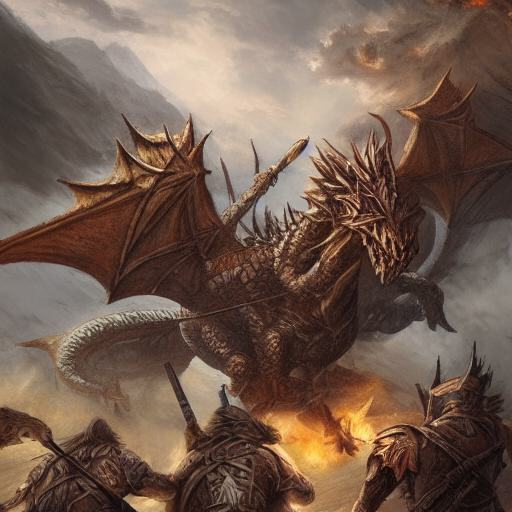
\includegraphics[width=\columnwidth]{introduction/what is a tabletop rpg}
    In tabletop role-playing games like Rise, you play a specific character of your own design.
    Your character can try to do anything you can imagine in a world that the game master, or GM, creates.
    Of course, you won't always succeed.
    The details of your character's capabilities are defined in the pages ahead; when you're done creating a character, it will have a personality of its own, along with strengths, weaknesses, and special abilities.
    Usually, your character will go on adventures with other characters, each of which is played by other players.
    Together, you will create and experience a story with the Game Master, or GM, who defines the universe that the player characters inhabit.

    \subsection{Describing Actions}
        Most of the time, when you're playing a game of Rise, you simply describe what you want your character to do.
        For example, you can say that your character steps out of their room in the inn and walks over to knock on a friend's door.
        Although Rise has rules that could govern some aspects of that scenario, such as an Awareness check to see if your friend notices you knocking, you wouldn't usually reference those rules explicitly.
        Even in the unlikely scenario that your friend doesn't notice you knock the first time, you can just knock again, so there's no point in worrying about the details.
        If something seems reasonable, it probably is, and you don't need to worry about the fiddly bits.

        Sometimes, when you describe what your character tries to do, the action has a narratively relevant chance of failure.
        Instead of knocking on the door to say hi, you might only have time to bang on it once to warn your sleeping friend about an attack from assassins.
        In that case, there's some chance that your friend is sleeping too deeply to notice the noise the first time you knock.
        You could try knocking again, just like in the first scenario, but in this scenario that failure would cost you valuable time to survive the attack.
        In that scenario, you would roll a die to determine whether you succeed in your action - or in this case, whether your friend would succeed in their attempt to notice you.

    \subsection{Using Specific Abilities}
        Instead of describing broadly what you want to have happen, you might choose one of a list of clearly defined abilities that your character can use.
        Every character has specific abilities unique to them, such as a wizard's spells known.
        There are also a number of simple abilities that anyone can use, such as the \ability{dirty trick} or \ability{trip} abilities.
        These universal abilities attempt to adequately describe a wide variety of reasonable improvised actions that you might try to use in combat.

        Explicitly defined abilities have rules for determining what happens when you use them.
        Some abilities, such as attacks in combat, require rolling dice to determine how effective they are.
        Of course, you can use your character's abilities at any time, not just in combat.
        Abilities such as the \spell{create water} or \spell{distant hand} spells can be used to solve other kinds of problems entirely.

    \subsection{Rolling Dice}
        Eventually, you'll have to determine whether something succeeds or fails.
        This can happen as part of using a specific ability that tells you exactly what to roll, or because you tried to narrate your character taking an action that has a dramatically relevant chance of failure.
        In either case, you'll roll a single ten-sided die, also known as 1d10.
        You'll add some modifier that represents how skilled your character is at the particular thing that they are trying to do.
        At the GM's discretion, they may also give the roll an extra bonus or penalty based on the circumstances that your character is in.
        If your die roll is high enough, your character succeeds at whatever they were trying to do.
        Otherwise, your character fails, which may sometimes have additional consequences.

        In Rise, it's entirely possible for characters to be so skilled that they succeed at what they are trying to do even if you roll a 1.
        Likewise, there are tasks that are so obviously impossible for your character that they cannot possibly succeed.
        In those cases, there's no reason to roll!
        Of course, the GM is the final arbiter of whether rolling is necessary.
        They may have information that the players do not.

    \subsection{Why Use So Many Rules?}
        
\includegraphics[width=\columnwidth]{introduction/so many rules}

        Tabletop role-playing games attempt to create rules to define how their universe works.
        Some games are intentionally vague or minimalist about their rules, which can be fun!
        Simple games are easy to start playing, and they try to avoid getting in the way of good role-playing.
        However, Rise takes a different approach.
        It spends a lot of effort - and words - attempting to define an internally consistent universe, and creating a large number of specific abilities that can be used in that universe.
        There are a few important advantages to taking this approach: establishing expectations, supporting multiple play styles, and assisting the GM.

        \subsubsection{Establishing Expectations}
            Different people can have very different ideas about what is realistic - or narratively appropriate - in a made-up fantasy universe.
            To some people, kicking in the tavern door and starting a brawl is just some good clean fun, and you'll take a few good punches and then laugh about it later that evening over drinks.
            But to other people, that might sound like a good way to find yourself imprisoned for the foreseeable future with all of your possessions confiscated by the town guard.
            Another interpretation of that scenario might see the brawler seriously injured with a broken bottle in the eye, leaving them partially blinded for weeks - or indefinitely.

            All of those ideas are valid, and they each match the narrative of a particular type of story.
            However, it's important that everyone sitting at a table and playing a game agrees about what to expect.
            Players can get confused or frustrated when their actions have consequences that feel arbitrary or unfair.
            Generally, games are more fun if everyone in the game shares a common set of expectations and conventions.
            Otherwise, games can devolve into disagreements about what is or isn't reasonable.

            One way to establish these expectations is to use a rules system like Rise that defines some expectations explicitly.
            If the scenario above happened in Rise, the last outcome of an incapacitating bottle to the eye shouldn't normally be possible, since the rules explicitly define how injury works.
            Knowing what is and isn't possible can help give players and GMs a useful set of guardrails for what they try to do in the universe.
            It's relatively easy to get everyone to agree about simple things that regular human people have experience with, like how difficult it is to climb a tree.
            However, Rise is full of superhuman people and monsters, and eventually you'll need to figure out how far a barbarian as strong as Hercules can throw a bear.
            Having a single authoritative resource to consult can cut off long disagreements about details that are difficult or impossible to determine objectively.

            Of course, different games played with a flexible rules system like Rise can have very different tones and themes.
            Either of the first two scenarios in the tavern are still plausible in different games, and a GM can use house rules to make vital wounds have more long-term consequences if they want.
            Using a rules system like Rise can help, but it is not the full answer by itself.
            The GM and players always share responsibility for establishing expectations about what genre a game will be, and conforming to those expectations to the extent that it makes the game more fun.

        \subsubsection{Supporting Multiple Play Styles}
            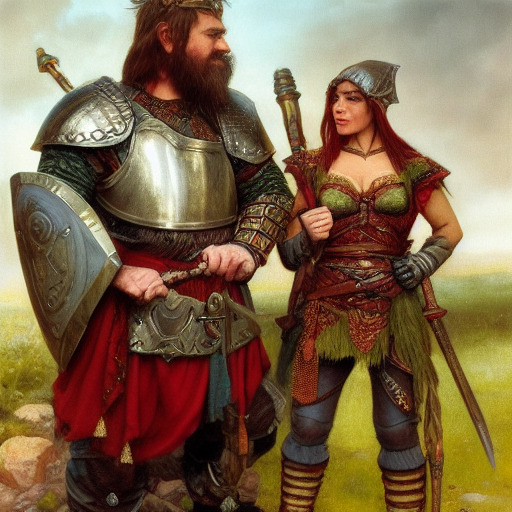
\includegraphics[width=\columnwidth]{introduction/multiple play styles}
            Some people deeply enjoy the process of role-playing itself.
            They enjoy the process of getting into a character and speaking in their voice, exploring their needs and desires, and building a narrative for them over time.
            These people often do not need the confines of a robust rules system, and can play equally well in games with minimal rules or none at all.

            Other people do not enjoy role-playing as an end in itself, or even at all.
            However, they may still enjoy the \textit{game} aspect of a role-playing game.
            Instead of playing a character for their personality and backstory, they may play a character for their unique mechanics and tactical advantages.

            Still other people may be interested in role-playing as a concept, but find it daunting.
            The blank page in front of you when you start painting a picture or writing an essay can be daunting, and that first step is often the hardest to take.
            Giving people a clearly defined set of abilities and specific tools for interacting with the world can enhance creativity by providing a safe space for interaction and experimentation.
            Even if you don't enjoy or feel confident in speaking in your character's voice, you can still engage with the narrative aspects of the adventure by casting a relevant spell or making a relevant skill check.
            People in this middle ground can sometimes enjoy deeper role-playing games while being feeling lost in role-playing games with minimal or nonexistent rules.

            One of the joys - and challenges - of Rise is drawing together people with very different desires and play styles to share a single experience.
            Rules-free role-playing games and tactical wargames can both have a narrower appeal than rules-heavy role-playing games like Rise, which try to provide something for everyone.
            You can run games with deep role-players alongside tactical gamers, and it can be a lot of fun.
            It does place a greater burden on the GM to provide the right ratio of content to keep everyone happy, and it does require the players to be patient when their preferred playstyle is put in the background to support the needs of other players.
            A well-blended game can also draw people out of their comfort zones slowly and safely over time as they observe and start to enjoy the playstyles of the other players in the game.

        \subsubsection{Assisting the GM}
            The Game Master carries an extra weight of responsibility to shape the flow of the game.
            Creating narratively consistent universes, appropriate challenges, and engaging storylines out of thin air is deeply challenging.
            If this job is too difficult, no one will want to do it, and then no one will play the game!
            Making the GM's job easier is a critical component of any role-playing game.

            There are several ways that Rise can make the GM's job easier.
            It provides information about the mechanics and tropes of the universe that the game takes place in, which helps establish expectations and resolve disputes that might come up during the game.
            It will provide a clear narrative foundation for the world and the characters in that world, which minimizes the up-front work required to run a game, once that section of the book is more complete.
            It will provide a wealth of pre-packaged challenges appropriate for players of any power level or play style, and advice for how to use those challenges appropriately, once that section of the book is more complete.
            The GM-focused sections are currently the most unfinished part of Rise, and this will be a more useful guide before Rise is done.

\section{What Makes Rise Different?}
    If you haven't played other tabletop role-playing games, feel free to skip this section.
    If you have, you may wonder what makes Rise unique in a crowded sea of games.
    Rise has five fundamental principles that differentiate it from other TTRPGs: minimal resource management, simultaneous combat, optional complexity, unbounded scaling, and a bounded action economy.

    \subsection{Minimal Resource Management}
        Many games make use of resources like mana, spell slots, or timed cooldowns to limit how often characters can use their abilities.
        These systems have fundamental problems that undercut the fun and flow of a TTRPG, and Rise essentially does not use resources to limit character ability usage.
        In Rise, characters can cast spells or use special attacks any number of times in a row without consuming resources.

        Some systems have resources that are designed to ebb and flow in the course of a typical combat.
        You might expend mana to use a powerful spell, and then regain mana over time by using weaker spells or fulfilling certain conditions.
        Alternately, you might use a spell and then wait some number of in-game turns before you can use that same spell again.
        This can be fiddly to track and hard to recover from if you forget what happened to your resource pool, which is why this approach is more common in video games than in TTRPGs.
        More importantly, this system has no clear way to handle ability usage outside of combat.
        It effectively gives unlimited ability usage when time is no obstacle, but only in an awkward and convoluted way.
        This category of system is unsuitable for Rise because it is too fiddly in combat and doesn't make sense out of combat.

        Some systems have finite-use resources that are tied to the expenditure of in-game time, such as taking long rests, or session breaks.
        You might spend a spell slot to use a powerful spell, and then be unable to cast that spell again until your character rests for some period of time.
        This can be manageable from a complexity perspective if the number of unique resources is small.
        However, it can get dangerously convoluted if characters have a large number of separate or partially interchangeable resource pools, such as using separate pools for individual spell levels.

        The real problem is that this limitation requires you to make your decisions based on not just the current situation, but also on your prediction of all future situations you will encounter before you have the opportunity to rest.
        This contributes significantly to the tactical complexity of deciding each individual action in combat, which slows down the pace of the game.
        It is also punishing to newer players who have less experience with the metagaming required to deduce how many resources an individual fight is worth.
        This strategic complexity is compounded if hit points are treated as an additional resource, since you now have to trade off the potential impact of one limited resource against another limited resource.

        Optimization of resource usage can be unintuitive and out of character, but failure to correctly manage your resources can leave you with no useful abilities remaining.
        This concern can be exacerbated if some characters are extremely resource-intensive while others have no meaningful resources to track.
        No one likes being forced to hide from a difficult fight or take only insignificant actions while your more resource-savvy or resource-independent allies continue using dramatic and powerful abilities.
        It can also add stress to the party dynamics when one character frequently asks for long rests after fights because they expended resources and no one else needs to rest.
        This category of system is unsuitable for Rise because it creates complexity in ways that detract from the fun and narrative of a game instead of adding to it.

        Rise does not use resources to limit normal actions in combat.
        The vast majority of spells, special martial attacks, and other abilities that affect enemies or your environment can be used any number of times.
        There are a small number of abilities with one-round cooldowns, and a universal ability that can only be used once per short rest.
        However, there is no time tracking in the system longer than ``next round''.
        Small cooldowns are a fine-grained balancing tool that allow characters to have powerful abilities which would have detrimental effects for the game if they could be used every turn.

        Rise does use a single universal resource, called ``fatigue'', that recovers based on long rests.
        This allows some opportunity for characters to invest extra effort into specific difficult fights, and to become tired after a long day.
        Normal damage taken during a fight is easily recovered after a ten minute rest.
        This means that you typically don't have to track state between fights.
        However, a GM can prevent that rest time with multiple sequential fights to increase difficulty and drama.

        Overall, Rise uses resource limitations very sparingly.
        This allows it to gain some of their benefits while avoiding the detrimental effects that come from making resource limitations a fundamental part of the system.

    \subsection{Simultaneous Combat}
        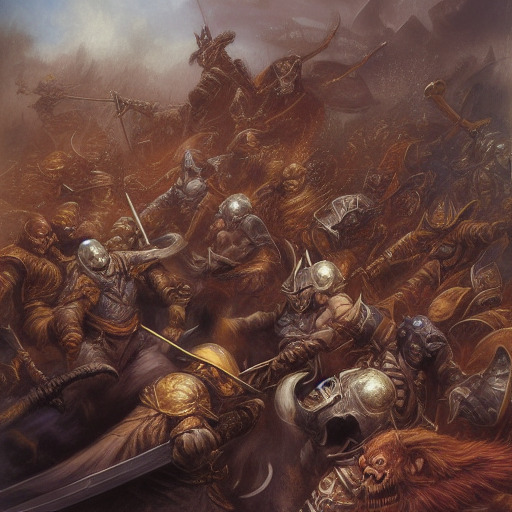
\includegraphics[width=\columnwidth]{introduction/simultaneous combat}
        In most TTRPGs, combat takes place in a series of turns.
        When your turn comes up, you take all of your actions, and then you wait through everyone else's turn until your turn comes again.
        This system has one foundational disadvantage: it is very, very slow.
        Rise uses a simultaneous combat system that dramatically increases the pace of combat.

        Imagine a typical 4-5 player game with 1-2 enemy groups using a traditional turn-based initiative system.
        In this scenario, you have to wait through about 5 turns before it comes back to your turn.
        This number can increase significantly in large-scale fights.
        Each of those 5 or so turns can meaningfully change the battlefield situation on its own by moving, weakening, or defeating various enemies and allies.
        The state of the battlefield at the end of last turn is often drastically different than the state of that battlefield at the start of your new turn.
        Player coordination can be challenging, since they must coordinate in the specific order assigned by the initiative system, and enemy turns can intervene to ruin coordinated plans.

        In theory, every player should accurately track the unfolding battlefield state through each of the intervening turns.
        That would mean everyone would know what to do when their turn comes up.
        In practice, many players find that difficult or impossible.
        Instead, at the start of each of their turns, they ask or try to figure out how the situation has changed.
        Not everyone asks this explicitly, but it must always be analyzed anew.

        Once a player understands the current battlefield state, they can finally decide their actions.
        This typically involves both movement and any number of sequential attacks, so there are many factors to consider.
        Everyone else must wait and do nothing while this happens.
        Once the active player has decided their actions, those actions must be fully rolled and resolved before combat can proceed.
        Even the next player in the initiative order may not be able to make accurate plans during this time, since the die rolls can change those plans.
        All of this combines to make even short combats take an hour or more, and six-person adventuring groups can feel dangerously bloated.

        Rise works differently.
        Combat in Rise is broken up into two phases: the movement phase and the action phase.
        During the movement phase, all creatures move simultaneously, and no attacks are possible.
        Characters can declare certain simple reactive movements like ``stay adjacent to this enemy'' to ensure that they end up in a reasonable position regardless of enemy actions.
        If the movements of characters conflict in impossible ways, initiative checks can temporarily force a linear order of resolution.
        Each player declares their own actions in an arbitrary order as soon as they decide them, so people are not forced to wait and do nothing while slower players contemplate their choices.
        Player coordination is easy, since all actions are happening together.

        During the action phase, players resolve their actions sequentially, but in an arbitrary order of the players' choice.
        This allows slower players to make their decisions when they are ready, while allowing faster players to resolve their actions first.
        Since movement during the action phase is rare, and enemies cannot unexpectedly move, players are typically able to decide their actions much more quickly and easily even when they have a large number of unique abilities to choose from.
        Once all players have resolved their actions, they learn what their enemies did.
        Those actions all resolve simultaneously, so enemy actions cannot interrupt player actions and vice versa.
        Attackers are always responsible for rolling instead of using ``saving throws'' or similar mechanics that force defenders to roll dice.
        All of this means that players can choose and resolve their actions simultaneously and efficiently, minimizing total time spent in combat while still allowing significant tactical complexity.

        The start of each phase still requires a general assessment from all acting players about the current state of the battlefield, which takes just as much time as the assessment in a classic initiative system.
        However, the time required for this tactical analysis only increases marginally as the number of players and enemies in the game increases.
        This allows Rise to handle large player counts or large enemy hordes without becoming glacially slow.
        Combat in Rise flows by quickly, making it much easier to balance time between combat and non-combat encounters within the same game session - or to run through multiple separate, individually challenging combats without sacrificing the pace and energy of the game.

    \subsection{Optional Complexity}
        Many games operate at a consistent level of complexity.
        Many rules-light games are always simple, and many rules-dense games are always complex.
        This is a perfectly reasonable design philosophy.
        Among other benefits, it makes it easy to know what to expect from the game, which helps give the game a well-defined niche.

        Rise is designed to allow players to choose their own level of complexity.
        This broadens its potential audience by allowing people with very different play styles or tolerances for complexity to enjoy the same game together.
        This goal is manifested in several key ways in Rise's design:
        \begin{itemize}
            \item Core gameplay is designed to be simple.
            \item Character creation is deeply interconnected.
            \item Complexity is not tied to narrative roles.
            \item Character power does not require complexity.
        \end{itemize}

        \subsubsection{Simple Core Gameplay}
            The core gameplay loop must be simple.
            You can contribute in combat by relying on one or two standard attacks that you use in all circumstances.
            In narrative situations, you can just roll the skills you have trained, and ignore other options.
            Engaging with the system more deeply than that is a choice, not a requirement.

        \subsubsection{Interconnected Character Creation}
            Character creation and build optimization is a better place to store complexity.
            Creating a Rise character involves a number of decisions, each of which can have nuanced ramifications on other aspects of the system.
            If you are just trying to build a character that matches a desired narrative, you can generally approach each decision in isolation.

            For example, you can decide that your character is intelligent and agile but not very strong or durable, because that is the concept you want.
            That decision has consequences, such as changing how many trained skills you have and what your defenses are.
            If you approach each decision sequentially, each one is relatively easy to make, and doesn't require deep system knowledge.
            On the other hand, trying to mathematically optimize a character requires thinking about many aspects of the system at once.
            This results in a system that is easy to learn but hard to master.

            Even for simple characters, the process of character creation is still one of the most complicated aspects of Rise.
            That is why Rise provides (or will provide, once that section is done) an extensive selection of premade characters for a wide variety of narrative archetypes.
            Each premade character includes advice for how to play that character and level them up.
            The premade characters make the system more accessible to people who don't want to to deal with the complexity of creating a character from scratch.

        \subsubsection{Complexity and Narrative}
            Complexity and simplicity should not be directly connected to a character's concept or narrative.`
            For example, it would be a bad idea to define a system where martial characters are simple and spellcasters are complicated.
            Both of those are rich and evocative narrative constructs.
            Many people who don't enjoy complexity will want to play spellcasters, and many people who enjoy complexity will want to play martial characters.
            Gameplay complexity must be more finely tuned and localized than those sweeping strokes.

            In Rise, gameplay complexity is generally generated by acquiring a large number of increasingly situational abilities.
            Every class has some archetypes that grant additional abilities known and some archetypes that grant additional passive abilities.
            If you like having a lot of unique abilities, you can have a high Intelligence to maximize your insight points, and focus on learning spells and maneuvers that attack your enemies or have situational effects.
            If you like minimizing complexity, you can instead choose archetypes or learn spells that simply grant you passive benefits, and focus on one or two standard attacks that you specialize in.
            Some feats give you new abilities and new circumstances to pay attention to that make you more effective, while others simply increase your passive statistics and defenses.

            Rise specifically handles complexity for martial characters and spellcasters slightly differently.
            Martial characters in Rise typically have fairly simple individual abilities.
            However, they can use those abilities with a variety of meaningfully different weapons.
            A martial character with four unique attacks and three different weapons has twelve different options in combat.
            In addition, martial characters can typically make better use of universal abilities, such as shoving and grappling.

            Spellcasters have more complex and varied individual abilities.
            They also tend to have more abilities that have significant narrative effects.
            However, their abilities are more isolated.
            There is no spellcaster equivalent of martial weapons that would multiply their number of distinct abilities in combat.
            The result of this design is that both martial characters and spellcasters can be very simple or very complicated.
            However, they approach complexity in different ways, ensuring that they feel narratively distinct.

        \subsubsection{Complexity and Power}
            All of this customization of complexity would be mostly pointless if complexity was strongly correlated with character power.
            If exceptionally complicated or hyper-specialized characters were obviously and consistently more effective than other characters, it would push everyone to use those characters.
            Rise structures the tradeoffs between gaining raw power and gaining additional options balanced enough that neither is always superior.

            There will always be some benefit from build optimization and system mastery.
            Players who are deeply familiar with Rise will be able to build characters with more relevant strengths and fewer relevant weaknesses.
            However, the gap between optimized characters and ``normal'' characters is limited.
            There will always be specific contexts where one character's mechanics are superior to another's.
            For example, a specialized defensive melee character may excel in a duel in a confined space.
            However, it may be irrelevant against cavalry archers on an open field.
            Characters in Rise cannot drastically change their capabilities each day, so they will always have moments to shine and moments of weakness.

    \subsection{Unbounded Scaling}
        
\includegraphics[width=\columnwidth]{introduction/unbounded scaling}
        Some systems uses bounded bonuses for accuracy or other game statistics.
        Bounded scaling means that every character of the same power level - or in some systems, of any power level - has a similar chance of success with any given skill check or attack roll.
        This can frequently cause narratively inappropriate and even comical events, and Rise explicitly rejects this philosophy.

        Imagine a typical party of four players, with one character being exceptionally skilled at a particular task.
        Perhaps the rogue is exceptionally skilled at lying, or a barbarian is exceptionally skilled at climbing.
        If ``exceptionally skilled'' only means that they have a \plus5 bonus on a d20 compared to \plus0 from the rest of the party, the exceptionally skilled character will only get the best result in the party half the time.
        The other half of the time, some other character with no relevant skills will meet or exceed the skilled character's result - sometimes by a dramatic margin.
        When failure compared to rank amateurs happens this often, it becomes hard to take seriously the idea that any character can be exceptionally skilled at anything.

        Rise characters can have dramatic statistical differences between each other, even at low levels.
        It uses a d10 as the fundamental die, which makes every bonus more significant.
        In addition, a 1st-level character can easily reach a \plus6 bonus with a skill check that is particularly relevant to their character.
        This means that a skilled character can beat a party of rank amateurs 80\% of the time, and at higher levels their success becomes completely guaranteed.
        Likewise, the difference in Mental defense between a powerful sorcerer and a cowardly rogue can allow mind-affecting attacks to almost always hit a rogue while almost never hitting the sorcerer.
        These statistical differences do not always grow with level, but they remain significant at every level.

        One advantage of systems with bounded scaling is that it is easier to guarantee that every character is relevant in any situation.
        Even if your character has no useful abilities of any kind, you might sometimes succeed on important actions through sheer luck.
        However, this design philosophy often breaks the symmetry between magical and non-magical characters.
        Magical characters can often use extremely specific and powerful abilities that are impossible for nonmagical characters to duplicate.
        If magical characters also have similar odds of success with all generic mechanics of the game, they will almost certainly have far more influence over the narrative of the game than any nonmagical character can hope to match.

        The philosophy of Rise is that it's okay for some characters to be irrelevant in specific contexts.
        It's good to give people time in the spotlight where their character's abilities help solve the specific problem that the group is facing when no other character could.
        Rise encourages that, and makes it impossible for one character to be relevant in \textit{all} contexts.
        Each character has their own strengths and weaknesses, and if you try to be good at everything, you'll fall behind people who specialize in a particular area.
        This will naturally rotate the spotlight between different characters, allowing each player to feel relevant and important in turn.

        This dramatic scaling is also used to govern the power of characters over time, in addition to the power of characters relative to each other.
        Rise attempts to model a massive power range for player characters.
        They are expected to start their journeys at level 1 as little more than commoners, and by level 21 they are effectively demigods who can alter the fate of entire worlds.
        This is a critical part of the narrative fabric of Rise, and it is reflected in the statistics and abilities of characters.
        If a level 1 kobold posed even a tiny threat to a level 21 character, the mechanics of the game would sabotage the purported narrative of power and growth.
        In Rise, overall character power doubles approximately every two to three levels.
        The system takes some care to avoid bloating numbers to unwieldy levels on this journey, and the use of the d10 as the standard die helps immensely.

    \subsection{Bounded Action Economy}
        It is dangerous to to give characters too many actions each turn.
        Each additional action a character can take increases how difficult it is for a player to decide what to do on their turn.
        In addition, each additional action increases the complexity of the change between the start of the turn and the end of the turn.
        This is especially risky with Rise's simultaneous initiative system, which combines the actions taken by all characters into a single resolution process.

        Rise places significant limitations on how many relevant actions each character can take on their turn.
        Generally, characters can only move during the movement phase and then take one significant action each turn.
        Some characters can use a minor action to accomplish something useful.
        However, that essentially marks the end of action economy scaling, even up to the maximum level.

        Detrimental effects that could deny actions are also heavily limited.
        Total action denial effects are only usable by high level characters, and even then they only work against weak enemies or enemies that have already been significantly damaged.
        Taking actions is fun, and sitting quietly while everyone else does things can be very frustrating.
        Similarly, completely removing an enemy's ability to act can easily remove the tension from a fight before it's actually over.


\chapter{How to Play}

\section{Saying What Your Character Does}
  There are two basic modes that you can use to describe how your character acts.
  You can describe in general terms what you want them to do, and let the GM figure out how to translate that into game mechanics.
  Alternately, you can say that you're using a specific ability or game mechanic, and let the GM figure out how that affects the narrative universe.

  Either approach is generally reasonable.
  Some people tend to prefer using one mode more often, and some GMs generally prefer to hear one mode.
  When in doubt, communicate at your table!

  \subsection{Describing Actions}
    With this style of communication, you describe what you want your character to do.
    For example, you can say that your character steps out of their room in the inn and walks over to knock on a friend's door.
    Although Rise has rules that could govern some aspects of that scenario, such as an Awareness \glossterm{check} to see if your friend notices you knocking, you wouldn't usually reference those rules explicitly.
    Even in the unlikely scenario that your friend doesn't notice you knock the first time, you can just knock again, so there's no point in worrying about the details.
    If something seems reasonable, it probably is, and you don't need to worry about the fiddly bits.

    Sometimes, when you describe what your character tries to do, the action has a narratively relevant chance of failure.
    Instead of knocking on the door to say hi, you might only have time to bang on it once to warn your sleeping friend about an attack from assassins.
    In that case, there's some chance that your friend is sleeping too deeply to notice the noise the first time you knock.
    You could try knocking again, just like in the first scenario, but in this scenario that failure would cost you valuable time to survive the attack.
    In that scenario, you would roll a die to determine whether you succeed in your action - or in this case, whether your friend would succeed in their attempt to notice you.

  \subsection{Using Specific Abilities}
    Instead of describing broadly what you want to have happen, you might choose one of a list of clearly defined abilities that your character can use.
    Every character has specific abilities unique to them, such as a wizard's spells or a fighter's maneuvers.
    There are also a number of simple abilities that anyone can use, such as the \ability{grapple} or \ability{trip} abilities.
    These universal abilities attempt to adequately describe a wide variety of reasonable improvised actions that you might try to use in combat.

    Explicitly defined abilities have rules for determining what happens when you use them.
    Some abilities, such as attacks in combat, require rolling dice to determine how effective they are.
    You can use your character's abilities at any time, not just in combat.
    Abilities such as the \spell{create water} or \spell{distant hand} spells can be used to solve other kinds of problems entirely.

\section{Rolling Dice}
  When you need to determine whether something succeeds or fails, you roll a die.
  This can happen as part of using a specific ability that tells you exactly what to roll, or because you tried to narrate your character taking an action that has a dramatically relevant chance of failure.
  In either case, you'll roll a single ten-sided die, also known as 1d10.
  You'll add some modifier that represents how skilled your character is at the particular thing that they are trying to do.
  At the GM's discretion, they may also give the roll an extra bonus or penalty based on the circumstances that your character is in.
  If your die roll is high enough, your character succeeds at whatever they were trying to do.
  Otherwise, your character fails, which may sometimes have additional consequences.

  In Rise, it's entirely possible for characters to be so skilled that they succeed at what they are trying to do even if you roll a 1.
  Likewise, there are tasks that are so obviously impossible for your character that they cannot possibly succeed.
  In those cases, there's no reason to roll!
  Of course, the GM is the final arbiter of whether rolling is necessary.
  They may have information that the players do not.

  In some cases, you roll multiple dice at once.
  This generally happens when you deal damage in combat.
  A collection of dice is called a \glossterm{dice pool}.
  Dice pools are written with the number of dice, followed by ``d'', followed by the size of dice to roll.
  For example, 2d6 means you roll two six-sided dice.

\section{Making Checks}\label{Checks}\label{Making Checks}
  A \glossterm{check} is a roll that you make to try to accomplish a task.
  For example, climbing a wall or remembering an obscure piece of trivia may require a check.
  Unlike an \glossterm{attack}, the difficulty of a check is not measured by the defense of another creature or object.
  Instead, it depends on the task itself.

  To make a check, roll 1d10 and add your modifier with the check.
  You compare that result to a \glossterm{difficulty value} that represents the difficulty of the task.
  The more difficult the task, the higher the \glossterm{difficulty value} will be.
  If your result is equal to or higher than the \glossterm{difficulty value}, the check succeeds.
  This usually means you accomplish a task successfully.
  Otherwise, the check fails.
  This usually means that nothing happens, though sometimes there are specific consequences for failure.

  \subsection{Critical Success}
    If your check result is at least 10 higher than the \glossterm{difficulty value}, your check is a \glossterm{critical success}.
    Some checks have a special effect on a critical success.
    For example, a critical success while climbing means you move twice as quickly.

  \subsection{Standard Difficulty Values}\label{Standard Difficulty Values}
    Most checks are made against a fixed \glossterm{difficulty value} that represents how hard the task is.
    Detailed rules for determining difficulty values in specific circumstances can be found in the Expanded Skills chapter from the Tome of Guidance.
    However, most of the time, it's not worth the effort to consult charts and tables to figure out how hard a task is.
    Instead, you can estimate it based on the guidelines below.

    \begin{itemize}
      \item Easy (DV 0): Only an exceptionally incompetent or impaired person could possibly fail a DV 0 check. For example, this includes walking on rough ground without tripping (Balance) or noticing that a yelling, red-faced person is angry (Social Insight).
      \item Average (DV 5): A typical human with no relevant skills should still succeed at a DV 5 check without much issue. However, it would be possible to fail in a stressful situation where time is limited if the person had no relevant training. For example, this includes climbing a ladder (Climb) or hearing the topic of a nearby conversation in a crowded bar (Awareness).
      \item Hard (DV 10): A typical human with no relevant skills might succeed at a DV 10 check, but only if they were very lucky or had a lot of time on their hands. An experienced practicioner might fail infrequently in stressful circumstances, but a world-class expert would never fail. For example, this includes swimming in fast-moving water (Swim) or providing first aid to mitigate a barely lethal wound (Medicine).
      \item Very Hard (DV 15): Only an experienced practicioner could succeed at a DV 15 check, and they would still need to get lucky if they were in a rush. Even a world-class expert at the peak of real-world human potential could fail, but only rarely. For example, this includes picking a well-made lock (Devices) or holding your breath for eight minutes while staying still (Endurance).
      \item Almost Impossible (DV 20): A world-class expert like an Olympic medalist could succeed at a DV 20 check if they were lucky or patient. Succeeding consistently at tasks of this difficulty requires superhuman capabilities. For example, this includes climbing a weathered natural rock wall without equipment (Climb) or squeezing through a space with a diameter of only half a foot (Flexibility).
      \item Impossible (DV 25\add): No real-world human can succeed at a DV 25 check. This sort of feat is only possible for high-level Rise characters who have explicitly surpassed ordinary limitations. For example, this includes running at full speed along a slack rope (Balance) or climbing a sheer glass pane (Climb).
    \end{itemize}

  \subsection{Trying Again}
    You can think of checks as being broadly divided into two categories: checks that give you information, and checks that cause a change in the world around you.
    In general, you can retry checks that change your environment indefinitely until you succeed.
    The only major limiting factor to those checks is that failure sometimes also changes your environment in ways that may punish your failure or make it impossible to retry the check.
    For example, if you are trying to climb a cliff, you can keep trying until you succeed, but you may take \glossterm{falling damage} from falling off while halfway up the cliff.

    You generally cannot retry checks that give you information unless the situation changes in a way that is relevant to your check.
    This generally means that you must learn new information before making the check again.
    For example, if you've already examined a creature to determine whether they are disguised, you can't keep just keep staring that creature to make sure.
    However, if you splash the creature with water which washes away some makeup, you can try again now that you have more information.

    % TODO: it would be nice if this wasn't necessary
    In addition, checks that require a free action to make can never be made more than once for the same purpose within a round.

  \subsection{Opposed Checks}
    An opposed check involves multiple creatures competing to get the highest result.
    In case of a tie, all tied creatures roll again to break the tie.
    Usually, the creature with the highest result succeeds, while all other creatures either fail completely or simply succeed less effectively depending on the situation.

    Some opposed checks involve multiple creatures using the same skill to see who does the best job.
    For example, a climbing race up a wall might involve each participant rolling a Climb check, or you might make a Strength check to hold a door closed while another creature tries to shove it open.
    Alternately, it can involve creatures rolling opposite skills.
    For example, if you are trying to hide, you roll a Stealth check opposed by the Awareness check of any creatures who could notice you.

    Not all opposed checks require all participants to roll at the same time.
    For example, a creature who creates a disguise rolls the Disguise check at the time that the disguise is created.
    A creature who tries to notice the disguise would roll their Awareness check at the time they see the disguised creature.

  \subsection{Extended Checks}\label{Extended Checks}
    An \glossterm{extended check} is a \glossterm{check} that represents your character taking some action over a prolonged period of time.
    You cannot use abilities like \ability{desperate exertion} to modify the results of an extended check.
    If your modifier changes over the course of the task, use your lowest modifier at any point during the task.

  \subsection{Hidden Checks}
    The GM can always make checks on your character's behalf without telling you.
    Generally, this is used for observation-based skills.
    For example, it's very suspicious if the GM tells you to make an Awareness check and then tells you that you don't see anything interesting.
    One of the ways a GM can avoid that is by simply rolling a check on behalf of your character and only telling you the result if you succeed.

  \subsection{Helping On Checks}
    You can help an \glossterm{ally} make a check.
    To help an ally, you make a check of the same type against a \glossterm{difficulty value} that is 5 lower than the regular difficulty value.
    This has the same requirements, including time and physical contact, as the check would have if you made it yourself.
    For example, to help an ally climb a cliff, you must be able to touch your ally to guide them up.
    Success means that the ally gains a \plus2 bonus to the check.

    Multiple creatures can try to help the same person.
    At the GM's discretion, there may be a practical limit to how many people can assist with the same task.
    The bonus from multiple creatures helping does not stack.
    It just makes it more likely that the helping attempt will succeed.

  \subsection{Checks for Timed Tasks}
    For every 5 points by which you beat the \glossterm{difficulty value} to accomplish a timed task, the time required is usually halved.
    This only applies for tasks that have a base time requirement of at least one minute, if the GM agrees that it is relevant, and if there are no other specific ways in which your result is improved with higher check results.

\section{Defining the Undefined}
  This book does not attempt to include specific rules for every aspect of a realistic world.
  Unless defined otherwise - or if it's not worth the effort to look up Rise's exact rules in the flow of a game - you should assume that the universe works more or less like the real world does, and as long as everyone agrees that something is reasonable, it's not worth worrying about in more detail.

  For example, Rise does not have specific rules for how long it takes to eat a meal, the arc that a thrown ball takes through the air, or how much extra weight a well-made chandelier can hold without breaking.
  It's possible to imagine situations where each of those might be important to a game, however, so you'll have to guess what would be reasonable as obscure situations arise.
  The Game Master has the final word when defining ambiguities like this.

  \subsection{Resolving Ambiguity}\label{Resolving Ambiguity}
    When the rules are ambiguous about how they apply to you and no other creature, you decide how to resolve that ambiguity.
    For example, if an ability causes you to remove one of your \glossterm{vital wounds}, and you have more than one vital wound, you choose which vital wound is removed.
    When the rules are ambiguous in any other situation, the GM decides how to resolve that ambiguity.
    This includes situations where multiple creatures are relevant and situations where no particular creature is relevant.


\chapter{Characters}\label{Characters}

This chapter describes how individual characters in Rise are defined, including their statistics.
For context about how characters act in combat, see \pcref{Combat}.
For context about how characters act more generally, see \pcref{Adventuring}.

Some of the information in this chapter won't fully make sense until you've read future chapters.
You can either skim past terms you don't yet understand or look them up as you go along.

\section{Attributes}\label{Attributes}

  Each character has six \glossterm{attributes}: Strength (Str), Dexterity (Dex), Constitution (Con), Intelligence (Int), Perception (Per), and Willpower (Wil).
  These attributes have a wide range of effects on a character's core statistics.

  Each attribute represents a character's raw talent in that area.
  A 0 in an attribute represents average human capability.
  That doesn't mean that every commoner has a 0 in every attribute; not everyone is average, after all.
  Player characters have an average attribute higher than 0 because they are exceptional individuals.
  For details about determining your attributes, see Step 4 of Character creation, \pref{Step 4: Attributes}.

  Your attributes can increase after character creation, such as by reaching level 3 (see \pcref{Character Advancement and Gaining Levels}).
  Increasing your attributes generally changes all of their effects appropriately.

  \subsection{Strength (Str)}\label{Strength}
    {
      Strength measures your muscle and physical power.
      Characters with a high Strength tend to have strong offensive capabilities with nonmagical abilities, and prefer wearing heavier armor.
      It has the following effects:
      \begin{raggeditemize}
        \item Strength determines how much you can carry (see \pcref{Weight Limits}).
          You generally need a Strength of at least 1 to wear heavy body armor.
        \item You add your Strength to your \glossterm{mundane power} (see \pcref{Power}).
        \item You add your Strength to your level to determine your \glossterm{brawling accuracy} (see \pcref{Brawling Accuracy}).
        \item A very high Strength can allow you to use \weapontag{Heavy} weapons in one hand (see \pcref{Weapon Tags}).
        \item If your Strength is positive, you reduce your \glossterm{encumbrance} from \glossterm{armor} by an amount equal to your Strength (see \pcref{Encumbrance}).
        \item You add your Strength to Strength-based \glossterm{skills}: Climb, Jump, and Swim (see \pcref{Skills}).
      \end{raggeditemize}
    }

  \subsection{Dexterity (Dex)}\label{Dexterity}
    {
      Dexterity measures your hand-eye coordination, agility, and reflexes.
      Characters with a high Dexterity tend to have strong defensive capabilities, and prefer wearing lighter armor.
      It has the following effects:
      \begin{raggeditemize}
        \item You add your Dexterity to your Armor defense.
          This bonus is halved if you use medium or heavy armor (see \tref{Armor and Shields}).
        \item You add your Dexterity to your Reflex defense.
        \item You add your Dexterity to Dexterity-based \glossterm{skills}: Balance, Flexibility, Ride, Sleight of Hand, and Stealth (see \pcref{Skills}).
      \end{raggeditemize}
    }

  \subsection{Constitution (Con)}\label{Constitution}
    {
      Constitution represents your health and stamina.
      Characters with a high Constitution tend to have strong defensive capabilities.
      It has the following effects:
      \begin{raggeditemize}
        \item Your Constitution increases your \glossterm{hit points}, as defined by your class (see \pcref{Classes}).
        \item You add your Constitution to your \glossterm{fatigue tolerance} (see \pcref{Fatigue}).
        \item You add your Constitution to your Fortitude defense.
        \item You add your Constitution to the Constitution-based \glossterm{skill}: Endurance (see \pcref{Skills}).
      \end{raggeditemize}
    }

  \subsection{Intelligence (Int)}\label{Intelligence}
    {
      Intelligence represents how well you learn and reason.
      Characters with a high Intelligence tend to have more options and special abilities.
      It has the following effects:

      \begin{raggeditemize}
        \item If your Intelligence is positive, you gain a number of \glossterm{trained skills} equal to your Intelligence (see \pcref{Trained Skills}).
        \item You add your Intelligence to the number of \glossterm{insight points} you gain (see \pcref{Insight Points}).
        \item You add your Intelligence to Intelligence-based \glossterm{skills}: Craft, Deduction, Disguise, Knowledge, and Medicine (see \pcref{Skills}).
      \end{raggeditemize}

      \par Creatures incapable of complex cognition and speech, like animals, have an Intelligence of \minus6 or lower.
      Creatures capable of speech have an Intelligence of at least \minus5.
    }

    \subsubsection{Changing Intelligence}\label{Changing Intelligence}
      When your Intelligence permanently increases, you also permanently gain an additional insight point and trained skill.
      Temporary Intelligence modifiers, such as from magic items, do not affect your insight points or trained skills.

  \subsection{Perception (Per)}\label{Perception}
    {
      Perception describes your ability to observe and be aware of your surroundings.
      Characters with a high Perception tend to have strong offensive capabilities.
      It has the following effects:
      \begin{raggeditemize}
        \item You add your Perception to your level to determine your \glossterm{accuracy} with almost all attacks (see \pcref{Accuracy}).
        \item You add your Perception to Perception-based \glossterm{skills}: Awareness, Creature Handling, Social Insight, and Survival (see \pcref{Skills}).
      \end{raggeditemize}
    }

  \subsection{Willpower (Wil)}\label{Willpower}
    {
      Willpower represents your ability to endure mental hardships.
      Characters with a high Willpower tend to be better at attacking with and defending against magical abilities.
      It has the following effects:
      \begin{raggeditemize}
        \item You add your Willpower to your \glossterm{magical power} (see \pcref{Power}).
        \item You add your Willpower to your Mental defense.
      \end{raggeditemize}
    }

\section{Combat Statistics}\label{Combat Statistics}

  \subsection{Accuracy}\label{Accuracy}
    Your accuracy with an \glossterm{attack} is the number that you add to the \glossterm{attack roll} (see \pcref{Attack Rolls}).
    Your base accuracy is equal to half the sum of your level and Perception.
    Many abilities can also modify your accuracy.

    \subsubsection{Brawling Accuracy}\label{Brawling Accuracy}
      Some abilities have the \abilitytag{Brawling} tag.
      Your base accuracy with those abilities is equal to half the sum of your level and Strength.
      This is called your \glossterm{brawling accuracy}, and an attack that uses your brawling accuracy is called a \glossterm{brawling attack}.
      Any ability that modifies your accuracy also modifies your brawling accuracy, but some abilities only affect your brawling accuracy.
      Many Brawling abilities are listed at \pcref{Special Combat Abilities}.

  \subsection{Damage Resistance}\label{Damage Resistance}
    Your \glossterm{damage resistance} measures how much damage you can shrug off without any effects.
    For details about how damage resistance is used, see \pcref{Taking Damage}.

    You do not intrinsically have any damage resistance.
    Wearing armor can significantly increase your damage resistance (see \pcref{Armor}).
    In addition, some class abilities and magic items can also increase it.

  \subsection{Defenses}\label{Defenses}
    When you are attacked, your defenses determine the value that the attacker needs to get on the attack roll in order to hit you (see \pcref{Attack Rolls}).
    The four defenses are described below.
    \begin{itemize}
      \item Armor defense (AD): Your Armor defense protects you from normal physical attacks, such as attempts to hit you with a sword.
        It is the most commonly used defense.
      \item Reflex defense: Your Reflex protects you from physical attacks that armor does not help against, such as pit traps or bolts of lightning.
      \item Fortitude defense: Your Fortitude defense protects you from attacks you have to physically endure or resist, such as poisons and life-draining spells.
      \item Mental defense: Your Mental defense protects you from attacks you have to mentally endure or resist, such as terrifying creatures and magical mind manipulation.
    \end{itemize}

    Your defenses are calculated in the following way:
    \begin{itemize}
      \itemhead{Armor} Half level \add Dexterity (modified depending on equipped armor) \add defense bonuses from equipped body armor and shield
      \itemhead{Fortitude} 3 \add Half level \add Constitution \add class defense bonus
      \itemhead{Reflex} 3 \add Half level \add Dexterity \add class defense bonus
      \itemhead{Mental} 3 \add Half level \add Willpower \add class defense bonus
    \end{itemize}
    Each defense may also have various bonuses or penalties applied by special abilities.

  \subsection{Encumbrance}\label{Encumbrance}
    Your encumbrance is a value that represents how much you are burdened by your armor (see \pcref{Armor}).
    You apply your encumbrance as a penalty to all Strength-based and Dexterity-based checks you make.
    If your Strength is positive, you reduce your encumbrance by an amount equal to your Strength.
    This cannot reduce your encumbrance below 0.

  \subsection{Hit Points}\label{Hit Points}
    Your \glossterm{hit points} measure how hard you are to seriously injure or kill.
    For details about how hit points are used, see \pcref{Taking Damage}.

    The way you calculate your hit points is defined by your class (see \pcref{Classes}).
    Increasing your level and Constitution will increase your hit points.
    Your maximum hit points can never be less than 1.
    If your maximum hit points would be reduced to 0 or less, you immediately die.

    \parhead{What Hit Points Represent} Hit points represent a combination of durability, luck, divine providence, and sheer determination, depending on the nature of the creature being damaged.
    When lose hit points from an orc with a greataxe, the axe did not literally carve into your skin without affecting your ability to fight.
    Instead, you avoided the worst of the blow, but it bruised you through your armor, the effort to dodge the blow fatigued you, or it barely nicked you through sheer luck -- and everyone's luck runs out eventually.

  \subsection{Power}\label{Power}
    Your \glossterm{power} is a general representation of how strong your abilities are.
    You have two types of power: your \glossterm{magical power}, which affects your \magical abilities, and your \glossterm{mundane power}, which affects your \glossterm{mundane} abilities (see \pcref{Magical and Mundane Abilities}).
    If you gain a bonus to your \glossterm{power}, and it does not specify which type of power it affects, it affects both your \glossterm{magical power} and your \glossterm{mundane power}.

    Your mundane power is equal to your Strength \add half your level.
    Similarly, your magical power is equal to your Willpower \add half your level.

    Many abilities have stronger effects depending on your \glossterm{power}, especially damaging abilities.
    % TODO: weapon damage wording
    For example, you gain a \plus1 bonus to your \glossterm{weapon damage} for every 2 power you have (see \pcref{Strikes}).

\section{Resources}\label{Resources}

  \subsection{Attunement Points}\label{Attunement Points}
    Many special abilities and magic items only function as long as a creature attunes to them.
    Attuning to an ability requires investing least one \glossterm{attunement point}.
    For details, see \pcref{Attuned Abilities}.

    You start with two attunement points.
    You gain additional attunement points as you gain levels (see \pcref{Character Advancement and Gaining Levels}).
    Some classes and abilities can grant additional attunement points.

  \subsection{Fatigue}\label{Fatigue}
    Thoughout the day, you can become fatigued by your exertions both in and out of combat.
    While \glossterm{hit points} are easy to restore, reducing your \glossterm{fatigue level} generally requires a \glossterm{long rest}.
    Fatigue is still easier to recover from than \glossterm{vital wounds}.

    \subsubsection{Fatigue Level}\label{Fatigue Level}
      Your \glossterm{fatigue level} measures how fatigued you are.
      A number of abilities and attacks can cause you to increase your fatigue level.
      The most common abilities that increase your fatigue level are the \textit{desperate exertion}, \textit{recover}, and \textit{sprint} abilities.
      All of those abilities are described in \pcref{Universal Abilities}.

    \subsubsection{Fatigue Tolerance}\label{Fatigue Tolerance}
      Becoming slightly fatigued is not immediately detrimental.
      Your fatigue level can be as high as 3 \add your Constitution without suffering any consequences (minimum 0).
      This value is called your \glossterm{fatigue tolerance}.
      Some abilities can increase your fatigue tolerance.

    \subsubsection{Fatigue Penalty}\label{Fatigue Penalty}
      You take a penalty to \glossterm{accuracy} and \glossterm{checks} equal your \glossterm{fatigue level} \sub your \glossterm{fatigue tolerance} (minimum 0).
      This penalty is called your \glossterm{fatigue penalty}.

    \subsubsection{Exhaustion}\label{Exhaustion}
      When your \glossterm{fatigue penalty} reaches \minus5, you fall \unconscious until your fatigue penalty is reduced below \minus5.
      Generally, this means that you are unconscious for 8 hours.

    \subsubsection{Recovering From Fatigue}
      When you finish a \glossterm{long rest}, your \glossterm{fatigue level} is restored to 0 (see \pcref{Resting}).
      There are no other ways to reduce your fatigue level.

    \subsubsection{Paying Fatigue Costs}
      Some abilities indicate that they cost a certain number of fatigue levels.
      That means that you increase your fatigue level by the given amount after the ability resolves.
      This means you do not suffer a \glossterm{fatigue penalty} from that extra fatigue while using the ability.
      You can even use abilities that cause you to drop unconscious from fatigue.

  \subsection{Insight Points}\label{Insight Points}
    You can spend \glossterm{insight points} to gain new special abilities.
    Your base insight points are equal to 1 \add your Intelligence (minimum 0).
    You gain additional insight points as you gain levels (see \pcref{Character Advancement and Gaining Levels}).
    Some classes and abilities can also grant insight points.

    Every class has at least one way to spend \glossterm{insight points} to learn additional abilities.
    These options are listed below.
    \begin{itemize}
      \item Barbarian: Combat styles, exotic weapons, and maneuvers
      \item Cleric: Mystic spheres and spells
      \item Druid: Mystic spheres, spells, and wild aspects
      \item Fighter: Battle tactics, combat styles, exotic weapons, and maneuvers
      \item Monk: Combat styles, exotic weapons, ki manifestations, and maneuvers
      \item Paladin: Mystic spheres and spells
      \item Ranger: Combat styles, exotic weapons, hunting styles, know your enemy, and maneuvers
      \item Rogue: Bardic performances, combat styles, exotic weapons, maneuvers, and trained skills
      \item Sorcerer: Mystic spheres and spells
      \item Votive: Combat styles, spells, maneuvers
      \item Wizard: Alchemical discoveries, metamagic, mystic spheres, portable workshop, scholastic insights, and spells
    \end{itemize}

    In addition, you can spend two \glossterm{insight points} to become a \glossterm{multiclass} character (see \pcref{Multiclass Characters}).

  \subsection{Trained Skills}\label{Trained Skills}
    You are trained in certain skills, which increases your bonus with those skills (see \pcref{Skills}).
    Your \glossterm{class} grants you a certain number of \glossterm{trained skills} from among the \glossterm{class skills} for that class.
    When you gain trained skills by any other means, you can choose any skill, not just your class skills.
    If your Intelligence is positive, you gain a number of trained skills equal to your Intelligence.
    Some abilities can also grant additional trained skills.

\section{Size and Weight}\label{Size and Weight}

  \subsection{Size Categories}\label{Size Categories}
    Your size affects your \glossterm{space} in combat, your speed with any \glossterm{movement modes} that depend on your size category's \glossterm{base speed}, your attributes, and how noticeable you are (see \pcref{Stealth}).
    These effects are shown on \trefnp{Size Categories}.
    Size categories are also relevant for determining weight (see \pcref{Weight Limits}).

    \begin{dtable*}
      \lcaption{Size Categories}
      \begin{dtabularx}{\textwidth}{l l l l l l l X}
        \tb{Size}   & \tb{Space}\fn{1} & \tb{Base Speed} & \tb{Weight Limits}\fn{2} & \tb{Reflex} & \tb{Stealth} & \tb{Weapons}             & \tb{Example Creature} \tableheaderrule
        Fine        & 1/4 ft.          & 10 ft.          & \minus4 Str              & \plus4      & \plus20      & \tdash                   & Fly                   \\
        Diminutive & 1/2 ft.          & 10 ft.          & \minus3 Str              & \plus3      & \plus15      & \tdash                   & Mouse                 \\
        Tiny        & 1 ft.            & 20 ft.          & \minus2 Str              & \plus2      & \plus10      & \tdash                   & Rat                   \\
        Small       & 2-1/2 ft.        & 20 ft.          & \minus1 Str              & \plus1      & \plus5       & \tdash                   & Cat                   \\
        Medium      & 5 ft.            & 30 ft.          & \tdash                   & \tdash      & \tdash       & \tdash                   & Human                 \\
        Large       & 10 ft.           & 40 ft.          & \plus1 Str               & \minus1     & \minus5      & \tdash                   & Ogre                  \\
        Huge        & 20 ft.           & 50 ft.          & \plus2 Str               & \minus2     & \minus10     & \weapontag{Massive} (10) & Hill giant            \\
        Gargantuan  & 40 ft.           & 60 ft.          & \plus3 Str               & \minus3     & \minus15     & \weapontag{Massive} (15) & Roc                   \\
        Colossal    & 80\add ft.       & 80 ft.          & \plus4 Str               & \minus4     & \minus20     & \weapontag{Massive} (20) & Great wyrm red dragon \\
      \end{dtabularx}
      1 Creatures can vary in space. These are simply typical values. \\
      2 This modifies Strength only for the purpose of determining a creature's \glossterm{weight limits} (see \pcref{Weight Limits}). \\
    \end{dtable*}

    \subsubsection{Space}\label{Space}
      A creature's \glossterm{space} is the area its body occupies while fighting.
      All humanoid species take up a 5-ft.\ by 5-ft.\ space in combat, which is a single \glossterm{square}.
      Normally, other creatures can't be in the space you occupy.
      Most creatures have a space significantly larger than the physical space their body occupies because they need room to maneuver in combat.

      Exceptionally large creatures can often attack at some distance from their core body thanks to long arms or other appendages.
      This is represented by making their space larger than their body alone would require.
      Even Colossal creatures can still only make melee attacks against adjacent foes - or more often, against smaller creatures sharing space with them.

    \subsubsection{Base Speed}\label{Base Speed}
      Each size category has a \glossterm{base speed} that indicates how far creatures of that size category can generally move.
      Most \glossterm{movement modes} use a speed equal to the base speed for a creature's size category.
      For context about movement in combat, see \pcref{Movement and Positioning}.

    \subsubsection{Other Effects}
      % TODO: record all of these and add them here
      A creature's size affects some additional skills and abilities.
      For example, larger creatures have a penalty to the Stealth skill (see \pcref{Common Stealth Modifiers}).
      The effects of unusual size are described in those skills and abilities.
      Unusually large or small creatures also have other special rules apply to them, as described below.

    \subsubsection{Very Small Creatures}
      \parhead{Space} If a creature takes up less than a single square of space, you can fit multiple creatures in that square.
      Ignoring flight, you can fit four Small creatures in a square, twenty-five Tiny creatures, 100 Diminutive creatures, or 400 Fine creatures.
      If the creatures can fly, the number of creatures that can fit into a space increases drastically.

      \parhead{Movement} Creatures two size categories smaller than you are not considered obstacles and do not hinder your movement.

    \subsubsection{Very Large Creatures}\label{Very Large Creatures}
      \parhead{Space} Very large creatures take up multiple squares. Anything which affects a single square the creature occupies affects the creature.

      \parhead{Movement} Creatures two size categories larger than you are not considered obstacles and do not hinder your movement.

      \parhead{Massive Weapons} Creatures that are Huge or larger have \weapontag{Massive} weapons, as shown in \trefnp{Size Categories}.

  \subsection{Weight Limits}\label{Weight Limits}

    \begin{dtable}
      \lcaption{Weight Limits by Strength}
      \setlength{\tabcolsep}{4pt}
      \begin{dtabularx}{\columnwidth}{X X X}
        \tb{Strength} & \tb{Carrying Capacity} & \tb{Push/Drag} \tableheaderrule
        -9            & Fine x4                & Diminutive x4 \\
        -8            & Fine x8                & Diminutive x8 \\
        -7            & Diminutive x2          & Tiny x2       \\
        -6            & Diminutive x4          & Tiny x4       \\
        -5            & Diminutive x8          & Tiny x8       \\
        -4            & Tiny x2                & Small x2      \\
        -3            & Tiny x4                & Small x4      \\
        -2            & Tiny x8                & Small x8      \\
        -1            & Small x2               & Medium x2     \\
        0             & Small x4               & Medium x4     \\
        1             & Small x8               & Medium x8     \\
        2             & Medium x2              & Large x2      \\
        3             & Medium x4              & Large x4      \\
        4             & Medium x8              & Large x8      \\
        5             & Large x2               & Huge x2       \\
        6             & Large x4               & Huge x4       \\
        7             & Large x8               & Huge x8       \\
        8             & Huge x2                & Gargantuan x2 \\
        9             & Huge x4                & Gargantuan x4 \\
        10            & Huge x8                & Gargantuan x8 \\
        11            & Gargantuan x2          & Colossal x2   \\
        12            & Gargantuan x4          & Colossal x4   \\
        13            & Gargantuan x8          & Colossal x8   \\
        14            & Colossal x2            & Colossal x16  \\
        15\plus\fn{1} & \tdash                 & \tdash        \\
      \end{dtabularx}
      1 To calculate the weight limits for a creature with epic Strength, double the number of objects it can carry and drag for every point of Strength beyond 14.
    \end{dtable}

    Your Strength determines how much you can carry or push, as shown in \trefnp{Weight Limits by Strength}.
    Your weight limits are measured in terms of how many objects or creatures of a given \glossterm{weight category} that you can carry or push at once (see \pcref{Weight Categories}).
    The limit of how much you can hold in your hands or on your body without suffering any penalties is called your \glossterm{carrying capacity}.
    If you need to move more weight than that, you can push or drag objects or creatures up your pushing and dragging limit as a standard action (see \pcref{Shove}).

    In general, it is not meaningful to consider the weight of any objects with a weight category lighter than your maximum weight category.
    If it matters, you can treat eight objects of one weight category as having an equivalent weight to a single object that is one weight category heavier.

    \parhead{Large Creatures} Unusually large or small creatures gain a bonus to their Strength for the purpose of determining their weight limits.
    For details, see \tref{Size Categories}.

    \parhead{Multi-Legged Creatures} The figures on \trefnp{Weight Limits by Strength} are for bipedal creatures.
    A creature with four or more legs can carry, push, or drag twice as many objects as a bipedal creature of the same Strength.

    \subsubsection{Weight Categories}\label{Weight Categories}
      Weight is generally measured in \glossterm{weight categories} rather than pounds or kilograms.
      Weight categories use the same terms as \glossterm{size categories}, as shown in \tref{Weight Categories}.
      In general, a creature's weight category is the same as its size category.

      Objects and creatures can also be either \glossterm{lightweight} or \glossterm{heavyweight}.
      Lightweight objects and creatures have a weight category that is one category lighter than their size category.
      Heavyweight objects and creatures have a weight category that is one category heavier than their size category.

      Objects that occupy only a small percentage of the space appropriate for their size category, such as swords, are usually lightweight.
      Objects that fully occupy the space appropriate for their size category, like boulders, are usually heavyweight.

      \begin{dtable}
        \lcaption{Weight Categories}
        \begin{dtabularx}{\textwidth}{l l X}
          \tb{Weight Category} & \tb{Falling Damage Die} & \tb{Average Weight} \tableheaderrule
          Fine                 & \tdash\fn{1}            & 1 oz.       \\
          Diminutive           & \tdash                  & 1/2 lb.     \\
          Tiny                 & 1d2                     & 2 lb.       \\
          Small                & 1d6                     & 15 lb.      \\
          Medium               & 1d8                     & 125 lb.     \\
          Large                & 1d10                    & 1,000 lb.   \\
          Huge                 & 2d6                     & 8,000 lb.   \\
          Gargantuan           & 2d8                     & 64,000 lb.  \\
          Colossal             & 2d10                    & 512,000 lb. \\
        \end{dtabularx}
        1. Creatures and objects with a Fine or Diminutive weight category have no falling damage dice and cannot cause falling damage.
      \end{dtable}

      % TODO: clarify that being immune to falling damage doesn't make you immune to damage from being fallen on.
  \subsection{Falling Damage}\label{Falling Damage}
    A falling creature or object descends by 300 feet at the end of each phase.
    If it hits an obstacle while falling, the falling creature or object takes falling damage.
    The obstacle it lands on takes half that damage, to a maximum amount of damage equal to the falling creature or object's hit points.

    This falling damage is based on the weight category of the falling object or creature.
    Each weight category has an associated falling damage die listed in \tref{Weight Categories}.
    For every 10 feet of the fall, the falling damage die is rolled once, to a maximum fall distance of 300 feet.
    If the total fall distance was less than 10 feet, no falling damage is dealt.
    For example, a Medium creature falling 50 feet would take 5d8 falling damage.

    If you fall intentionally, you treat your fall as being 10 feet shorter.
    If you fall after intentionally jumping, you measure falling damage from 10 feet lower than your height at the start of your jump, ignoring the maximum height you reached during the jump.

\section{Calculation Guidelines}
  This explains some general guidelines to follow when calculating character statistics.

  \subsection{Stacking Rules}\label{Stacking Rules}
    Usually, modifiers stack with each other, meaning that you add or subtract all of the modifiers to get the final result.
    However, some modifiers do not stack with each other, as described below.
    When bonuses don't stack with each other, you only apply the largest bonus.
    Likewise, when penalties don't stack with each other, you only apply the largest penalty.

    \begin{itemize}
      \item Effects from abilities with the same name do not stack.
      \item Enhancement bonuses do not stack with each other.
      \item If a creature gains the same condition multiple times, the effects do not stack, but each instance of the condition is tracked separately.
        The creature must remove all instances of the condition before the effects are removed.
      \item Multiple \magical effects that change a creature's \glossterm{size category} do not stack.
        If multiple magical effects both increase and decrease size, size increases offset size decreases on a one-for-one basis to determine the creature's final size.
      \item If you have two separate abilities which grant you a special sense with a particular range, such as \trait{darkvision} or \trait{blindsight}, you sum the range from both abilities to find your total range with that sense.
    \end{itemize}

  \subsection{Minimum and Maximum Modifiers}\label{Minimum and Maximum Modifiers}
    Some bonuses specify that they cannot increase the value beyond a given point.
    These bonuses must always be applied last, and cannot be combined with other bonuses to exceed the maximum value.
    If multiple bonuses specify different maximum values, use the lower maximum value.
    If a bonus with a maximum value is applied to a value that already exceeds the maximum value the bonus can provide, simply ignore the bonus and its maximum value.

    Similarly, some abilities have a minimum total modifier.
    The minimum is applied after all other modifiers.

  \subsection{Doubling and Halving}\label{Doubling and Halving}
    If you double any in-game value twice, it becomes three times as large.
    An additional doubling would make it four times as large, and so on.
    Likewise, if you halve any in-game value twice, it becomes one-third as large.
    For example, if you have two different abilities that double your \glossterm{power} with an attack, you triple your power with that attack.

    This also applies to calculations using real-world values, such as movement and distance, as long as you're calculating the effects of abilities.
    For example, if you have two different abilities that double your range with a spell, your total range with that spell is three times the spell's normal range.

    \subsubsection{Doubling Damage}
      If you double your damage with a dice pool, you roll the same number of dice and modify the result.
      This is different from a \glossterm{critical hit}, which changes the number of dice you roll.
      As a result, if you get a \glossterm{critical hit} with a double-damage attack, you roll twice as many dice and then double the result, which typically means you deal 4x your normal damage.

  \subsection{Changing Statistics}

    Your modifiers and defenses can change for many reasons.
    In general, all changes take effect immediately.

    It is not normally possible for a character to lose access to resources that require them to make choices, such as insight points or trained skills.
    If a character does somehow lose the prerequisites for choices they have made, such as if their Intelligence is permanently reduced, they immediately lose relevant abilities until they are within their new limits.

  \subsection{Rounding}
    In general, if you encounter a fractional number, you round it down.
    For negative numbers, this means rounding it away from 0, not towards 0.

\section{Character Creation}\label{Character Creation}

  Creating a character involves a mixture of thematic and mechanical decisions that will work together to create a fun character that is rewarding to play.
  As mentioned earlier in this chapter, there are four core systems for customizing your character's mechanics: class, attributes, skills, and species.
  In addition, there are five core thematic considerations when creating a character: concept, personality, motivation, background, and appearance.

  These decisions are described below in a order that makes sense for many characters, and full details for each decision are given after this initial list.
  It is essentially a sandwich, with narrative decisions wrapped around a central core of your character's mechanical components.
  However, you can make several of these decisions in any order, and you may find it easier to create a character in a different way.
  The only real limitation is that your skills should generally be the last mechanical choice you make, since they are strongly affected by your class and attributes.

  \begin{enumerate}
    \item Character concept: Describe your character with a short, simple phrase that captures their essence.
    \item Motivation and goal: Describe what your character wants.

    \item Species: Define your character's species.
    \item Attributes: Define your character's fundamental physical and mental potential.
    \item Class archetypes: Define your character's source of power.
    \item Insight points: Learn new abilities.
    \item Skills: Define your character's areas of non-combat expertise.

    \item Personality: Describe how your character acts and reacts to the world.
    \item Background: Describe what made your character become who they are now.
    \item Appearance: Describe what your character looks like.
    \item Alignment: Describe your character's moral compass.
    \item Name: Choose a name.
  \end{enumerate}

  \subsection{Step 1: Character Concept}

    Fundamentally, who is your character?
    You should think of a short phrase that describes the core concept behind the character you will create.
    It's best to think in broad strokes when creating a character concept.
    Your concept should be more than just a factual description of your species or what you do.
    It should be something that makes you memorable.
    Some sample character concepts are given below for inspiration.

    \begin{raggeditemize}
      \item Pragmatic wanderer
      \item Artistic pixie
      \item Mushroom-obsessed hermit
      \item Bumbling do-gooder
      \item Dim-witted bodyguard
      \item Cowardly storyteller
      \item Bear-barian
      \item Parsimonious law enforcer
      \item Peaceful naturalist
      \item Trigger-happy pyromaniac
      \item Heroic, simple-minded warrior
      \item Friendly necromancer
      \item Chaotic speed demon
      \item Pompous ex-noble
      \item Sarcastic mercenary
      \item Battle-scarred priest
      \item Ambitious arcane prodigy
      \item Charismatic musician
      \item Aloof scholar
      \item Blunt-spoken warrior
      \item Crazed prophet
      \item Polite warrior
      \item World-weary pirate
      \item Devout cultist
      \item Con artist with a heart of gold
    \end{raggeditemize}

  \subsection{Step 2: Motivation and Goal}
    Why does your character put in all of the effort that adventuring requires?
    They probably have a goal that they are trying to achieve, or an ideal that they are trying to embody.
    Writing down a specific goal or ideal can be helpful as an anchor point when defining the character.

  \subsection{Step 3: Species}
    It's often convenient to make your species your first mechanically relevant choice.
    Your species can have a strong effect on your personality and narrative, but it has a relatively small effect on your character's play style.
    It's also easier to know your species before you choose your attributes, since your species can slightly modify your attributes.

    Choose one of the eight common species options, or talk with your GM about choosing an uncommon species (see \pcref{Uncommon Species}).
    Record any specific abilities the species gives you on your character sheet, but if this is your first mechanical choice, you won't be able to finalize any of your statistics yet.
    You should also choose the languages that you can speak, since that is influenced by your species (see \pcref{Communication and Languages}).

  \subsection{Step 4: Attributes}\label{Step 4: Attributes}
    Your attributes are a good option for your second mechanically relevant choice.
    They have a large impact on your character's strengths and weaknesses, so it's useful to know them as soon as possible.
    They're also much easier to understand and finalize than your class archetypes.

    You have 8 points to distribute among your attributes.
    Increasing an attribute by 1 costs 1 point, and you can increase each attribute up to a maximum of 3.
    Instead of allocating points yourself, you can use one of the following three common attribute arrays:
    \begin{raggeditemize}
      % 3 + 2 + 2 + 1 = 8
      \item Standard: 3, 2, 2, 1, 0, 0
        % 3 + 3 + 2 = 8
      \item Specialized: 3, 3, 2, 0, 0, 0
        % 2 + 2 + 2 + 1 + 1 = 8
      \item Balanced: 2, 2, 2, 1, 1, 0
    \end{raggeditemize}

    Once you have chosen your attributes, add your species modifier to your attributes (if any).
    Then, record in your character sheet the various effects that your attributes have on your statistics.

    \subsubsection{Attribute Penalties}\label{Attribute Penalties}
      You can voluntarily take penalties to your attributes.
      If you reduce an attribute by a total of \minus1, you gain an additional \glossterm{trained skill} (see \pcref{Trained Skills}).
      If you reduce an attribute by a total of \minus2, you instead gain an additional \glossterm{insight point} (see \pcref{Insight Points}).
      You cannot gain these benefits from reducing more than two attributes below 0 in this way.
      In addition, you can never reduce an attribute below \minus2 in this way.

  \subsection{Step 5: Class and Class Archetypes}
    This is the most complicated choice you have to make for your character.
    It requires reading at least some of the Classes chapter to understand which classes are interesting to you.
    Class details can be found in \pcref{Classes}.

    You should choose one of the eleven classes, and apply all effects of choosing that as your \glossterm{base class}.
    Then, choose one of the five archetypes within that class.
    You gain the rank 1 ability from that archetype.

    When you reach levels 2 and 3, you'll choose new archetypes from the same class, becoming rank 1 in each of those archetypes as well.
    After that, you won't gain any more new archetypes when you gain levels.
    Instead, you'll just increase your rank in the three archetypes you already have.

    If you are particularly adventurous, this is also when you should choose if you want to be a multiclass character.
    Multiclass characters can gain archetypes from multiple classes.
    This does not increase the number of archetypes you know, so it does not directly increase your power.
    However, multiclass characters can be more specialized or more versatile than single-class characters, and can represent unusual character concepts.
    For details, see \pcref{Multiclass Characters}.

  \subsection{Step 6: Insight Points}
    Once you have chosen your class archetypes, attributes, and species, you know how many insight points you have, and can choose how to spend them.
    Don't forget to record on your character sheet how you spent each insight point.
    Otherwise, you might get confused later about why you have more spells known than you normally would.

    In some circumstances, you might want to delay spending your insight points until you are higher level.
    For example, a fighter/sorcerer multiclass character who wants to have both spells and maneuvers can't have access to both spells and maneuvers at level 1, so they wouldn't be able to spend insight points on both spells and maneuvers.
    You aren't forced to spend all of your insight points, so you can save them up for later.
    You can also talk to your GM about spending them at level 1 and then retraining those insight points once you are higher level.

  \subsection{Step 7: Skills}
    You should choose which skills you have as \glossterm{trained skills} (see \pcref{Skills}).
    Your \glossterm{class} gives you a certain number of trained skills from among its \glossterm{class skills}.
    The class skills for each class are summarized in \tref{Class Skills}.

    There are other ways to become trained in skills that are not part of your class.
    If your Intelligence is positive, you gain additional trained skills equal to your Intelligence.
    You can also spend \glossterm{insight points} to gain one trained skill per insight point (see \pcref{Insight Points}).
    Some abilities can grant additional trained skills.

    If you are untrained in a skill, your bonus with that skill is equal to half of its associated attribute (if any).
    If you are trained in a skill, your bonus with that skill is equal to 3 \add the higher of its associated attribute (if any) and half your level.
    Many abilities can increase or decrease your bonus with particular skills.

    The number of skills you can have trained, and which skills those are, depend on every preceding step, so it's a good place to finish.

    Sometimes, you might have more trained skills than you know what to do with, especially if you are still figuring out the details of your character concept.
    You aren't forced to decide all of your trained skills at level 1, so you can save them up and choose more trained skills when you level up.
    You can also talk to your GM about letting you decide your trained skills on the fly during the first game session or two based on what actions you take during the session.
    This can be a fun way to figure out what your character's personality is through the process of playing them.

  \subsection{Step 8: Starting Equipment}
    When you create a character, they can start with some basic items.
    Items have \glossterm{item ranks} that indicate the approximate rank that characters can reasonably get access to them.
    Typically, you can start with a single rank 1 item, up to three rank 0 items, and a standard adventuring kit.
    Individual campaigns or character backstories may significantly change what starting equipment is available, so check with your GM.

  \subsection{Step 9: Personality}

    How does your character behave?
    You should decide, in broad terms, what your character's personality is.
    This will change over time, especially as you start playing the character in the game, so you don't need to define everything perfectly.
    However, having a general sense of how your character behaves is helpful.

    For most games, it's important to have a personality that can tolerate working with others in a group.
    A character that is excessively aloof, moody, or obnoxious can make the game more difficult to enjoy for everyone.
    Likewise, a character who tries to speak for everyone or who repeatedly steals the spotlight from others can be frustrating to work with.
    You should figure out the right balance with your fellow players and your GM.\@

  \subsection{Step 10: Background}
    What happened in their character's past to make them the way that they are?
    What were their parents like, and where are they now?
    You don't have to have all of the answers when you first create a character, but it's good to have some idea.
    The richer your backstory, the more the GM can weave that into the narrative of the current story.
    Sometimes, it's fun to take a break from saving the world to go visit someone's grandma.
    For details about suggested backgrounds that have a strong effect on the game world, see \pcref{Backgrounds}.

  \subsection{Step 11: Appearance}
    What does your character look like?
    What would someone's first impression of them be?
    This can be helpful for understanding how other characters in the game world - or even monsters - would react to you.

  \subsection{Step 12: Alignment}
    Your character's alignment reflects their moral character: are they more inclined to good or evil, and to chaos or order?
    Alignments are described in more detail at \pcref{Alignment}.

  \subsection{Step 13: Name}
    What is your character's name?
    This choice can influence the tone your character will set in the game.
    If your name is Sir Patty Cakes or Shanky, the game is likely to be lighter and sillier in tone.
    Fancy fantasy-appropriate names like Ayala or Theodolus tend to push the game in a slightly more serious direction, especially if you make the daring choice to include a canonical last name.
    As always, stay in tune with what the GM and the other players are expecting.

\section{Alignment}\label{Alignment}
  A creature's general moral and personal attitudes can be represented by its alignment: lawful good, neutral good, chaotic good, lawful neutral, neutral, chaotic neutral, lawful evil, neutral evil, or chaotic evil.

  Alignment is a tool for developing your character's perspective.
  Like a character's class, it is intended to provide a canvas to inspire creativity, not a narrow window to constrain identity.
  Each alignment represents a broad range of personality types or personal philosophies, so two characters of the same alignment can still be quite different from each other.
  In addition, few people are completely consistent.

  \subsection{Aligned Characters}
    Alignment is a spectrum, not a binary.
    Some characters are defined as being ``good'' or ``evil'', but this is a broad definition with a great deal of variation.
    Only angels and demons are ``pure'' good or evil.

    Approximately half of the general population of the world is neutral between good and evil, with a quarter being good and another quarter being evil.
    This does not mean that a quarter of people are all saintly do-gooders and another quarter are all psychotic murders.
    It would be more accurate to say ``good'' people are simply the most altruistic quarter of the population.
    There are a rare few saints, but all good characters have some amount of selfishness in particular contexts.
    Likewise, evil characters may act altruistically in some situations still having a fundamentally selfish nature.

    A similar ratio exists for law and chaos.
    This means that the overall population follows the ratios given in \trefnp{Aligned Population Ratios}.
    Of course, these populations are not distributed equally in the world.
    In general, humanoid civilization tends to have more good and lawful characters, and monsters tend to be more chaotic and evil.
    The GM can give more context about how alignment is used in their specific world.
    Of course, the GM can also redefine good and evil itself, so talk with them if alignment is important to you or your character.

    Monsters have their typical alignments listed in their description.
    Even monsters who are listed as ``always good'' or ``always evil'' are not \textit{maximally} good or evil -- just good or evil enough to fall into that quartile.
    Many evil monsters can be perfectly reasonable if they are capable of speech, and will uphold bargains that serve their interests.
    Likewise, good monsters have their own objectives, and will not simply do whatever an adventuring party asks of them.

    \begin{dtable}
      \lcaption{Aligned Population Ratios}
      \begin{dtabularx}{\textwidth}{X X X X}
        \tb{Alignment} & \tb{Good} & \tb{Neutral} & \tb{Evil} \tableheaderrule
        \tb{Lawful}    & 6.25\%    & 12.5\%       & 6.25\% \\
        \tb{Neutral}   & 12.5\%    & 25\%         & 12.5\% \\
        \tb{Chaotic}   & 6.25\%    & 12.5\%       & 6.25\% \\
      \end{dtabularx}
    \end{dtable}

  \subsection{Good vs. Evil}
    Distinguishing good from evil is a deeply complex task.
    In a universe where angels, demons, and deities exist and interact with the affairs of mortals, being able to clearly define good and evil is important.
    For the purposes of Rise, good and evil are strictly defined according to the intentions of one's actions, not their eventual outcomes.
    Good intentions are altruistic, and evil intentions are selfish.

    This model for good and evil has limited value as a moral system for the real world, and it neglects several dimensions of morality that people might consider important.
    It is intentionally vague about what consistutes ``other beings'', and reasonable characters might disagree about how to consider the needs of non-humanoid living things like plants and animals.
    However, is a useful way to define alignment as a character trait and roleplaying tool.
    Good characters have recognizably different behaviors from evil characters, but they are not so intrinsically opposed that they can't coexist in the same group of adventurers.
    Evil characters may cause you problems if you get in their way, but no civilized area would allow simply killing evil on sight.

    \parhead{Good} Good intentions are altruistic.
    They are based on respect and empathetic consideration for other beings.

    A good character will try to learn what other beings want or need so they can help most effectively.
    They might try to keep everyone's spirits up with cameraderie and good humor, donate money whenever possible to help those in need, or dedicate their life to punishing criminals and protecting the innocent.
    Good characters may have significant disagreements about what actions are best, and not all care about some lofty ``greater good''.
    Some believe that self-sacrifice is noble, while many would say that it does more harm than good to neglect your own needs.
    There are many interpretations of altruism.

    Even an action with good intentions may have disastrous consequences.
    Unintentionally causing harm does not make a character evil, but good characters pay attention to the effects their actions have in practice.
    If a good character caused harm, intentionally or otherwise, they would try to rectify their mistake.

    \parhead{Evil} Evil intentions are selfish.
    They come from prioritizing one's own desires when that conflicts with the knowable needs and desires of other beings.

    An evil character will generally not care what other beings want or need unless they personally benefit from that knowledge.
    They might betray allies, break laws or abuse legal loopholes to gain an advantage, or bully other creatures into doing their bidding.
    Evil characters may take actions that help others and can even work effectively as a team, but their ultimate motivation is to help themselves or make themselves feel better, not to help others.

    \parhead{Neutral} Characters that are neutral between good and evil are neither consistently altruistic nor consistently selfish.
    Most neutral characters behave altruistically in some ways and selfishly in other ways -- either at different times, or about different aspects of life.
    They often have strong bonds to particular individuals who they care about selflessly, but are not altruistic in a general sense.

    Intentions that do not involve other beings are neither good nor evil.
    Similarly, actions taken to meet one's own mandatory needs are neither good nor evil.
    Wild animals may act primarily out of self-interest, but since they generally lack the capacity to recognize the needs and desires of other beings, they are considered neutral rather than good or evil.

  \subsection{Law vs. Chaos}
    \parhead{Law} Lawful characters value consistency.
    They obey rules that guide their actions.
    Some lawful characters draw their rules from external forces, such as serving a particular master or following the legal laws of the land.
    Other lawful characters follow rules they make for themselves.

    \parhead{Chaos} Chaotic characters value flexibility and freedom.
    They make decisions based on what they think or feel at the time, even if it is inconsistent with their previous statements or actions.

    \parhead{Neutral} Characters that are neutral between law and chaos are neither exceptionally consistent nor exceptionally inconsistent.
    They tend to be generally consistent but may change their minds under the right circumstances.
    Non-sapient beings such as animals are neutral rather than lawful or chaotic.

\section{Personal Appearance}\label{Personal Appearance}
  \begin{dtable!*}
    \lcaption{Species Age}
    \begin{dtabularx}{\textwidth}{l *{5}{>{\ccol}X}}
      \tb{Species} & \tb{Adulthood} & \tb{Middle Age} & \tb{Old}  & \tb{Venerable} & \tb{Maximum Age} \tableheaderrule
      Human        & 18 years       & 40 years        & 55 years  & 70 years       & \plus3d10 years \\
      % 50% longer than humans
      Dwarf        & 30 years       & 60 years        & 85 years  & 110 years      & \plus5d10 years \\
      % 4x longer than humans, scaling up to 5x/6x for old/venerable
      Elf          & 70 years       & 160 years       & 275 years & 420 years      & \plus3d\% years \\
      % 75% of human lifespan, scaling up for old/venerable
      Gnome        & 14 years       & 30 years        & 45 years  & 60 years       & \plus1d\% years \\
      % 50% longer than humans, scaling up to 2x/2.5x for old/venerable
      Half-elf     & 30 years       & 60 years        & 110 years & 175 years      & \plus7d10 years \\
      % Same as humans, scaling down for old/venerable
      Half-orc     & 18 years       & 40 years        & 50 years  & 60 years       & \plus3d10 years \\
      % 50% longer than humans
      Halfling     & 30 years       & 60 years        & 85 years  & 110 years      & \plus5d10 years \\
      % Same as humans, scaling down for middle+
      Orc          & 18 years       & 35 years        & 45 years  & 55 years       & \plus3d10 years \\
    \end{dtabularx}
  \end{dtable!*}

  \begin{dtable}
    \lcaption{Typical Height and Weight}
    \begin{dtabularx}{\columnwidth}{l *{2}{>{\lcol}X}}
      \tb{Species} & \tb{Average Height} & \tb{Average Weight} \tableheaderrule
      Human        & 5' 5''              & 140 lb. \\
      Dwarf        & 4' 2''              & 140 lb. \\
      Elf          & 5' 9''              & 120 lb. \\
      Gnome        & 3' 4''              & 50 lb.  \\
      Half-elf     & 5' 6''              & 140 lb. \\
      Half-orc     & 5' 9''              & 170 lb. \\
      Halfling     & 3' 1''              & 50 lb.  \\
      Orc          & 6' 0''              & 190 lb. \\
    \end{dtabularx}
  \end{dtable}

  \subsection{Age}
    The typical age for each species is listed in \trefnp{Typical Ages}.
    The Adulthood column indicates the minimum age for adulthood.
    Most adventurers are somewhere between adulthood and middle age.

    If you are old, you take a \minus2 penalty to \glossterm{checks} based on Strength, Dexterity, Constitution, and Perception.
    However, you gain a \plus2 bonus to \glossterm{checks} based on Intelligence and Willpower.
    If you are venerable, these modifiers change to \minus4 and \plus4 respectively.
    In general, player characters should not start as old or venerable age, but the GM can always allow it for specific campaigns if they want.

    When you reach venerable age, the GM secretly rolls your maximum age, which is the number from the Venerable column on \trefnp{Typical Ages} plus the result of the dice roll indicated on the Maximum Age column on that table.
    They record the result.
    If you reach your maximum age, you die of age-related illnesses or frailty at some time during that year.

  \subsection{Height and Weight}
    The typical height and weight for each species is listed in \tref{Typical Height and Weight}.
    The average man from each species is slightly taller and heavier than the average woman, but this is not a restriction for player characters.

\section{Backgrounds}\label{Backgrounds}
  Each character has a history from before the current campaign.
  This can include their childhood, family, previous occupations, and more.
  Backgrounds generally do not have direct effects on a character's statistics.
  Narratively, a background explains a character's statistics, not defines them.
  However, a character's background can still have a significant influence on how they interact with the world.

  Backgrounds can be summarized as a set of benefits and flaws.
  If you choose a background benefit, you must also choose a flaw.
  Some backgrounds internally provide both benefits and flaws.
  These are called mixed backgrounds, and taking them does not change how many benefit or flaw backgrounds you can choose.
  You generally shouldn't have more than one benefit and one flaw, or a single mixed background.

  Not every character should have a specific background with effects listed here.
  These backgrounds can significantly change how a character relates to the world.
  It's fine to have a simpler background to put more focus on other aspects of your character's narrative journey.

  At the GM's discretion, backgrounds can also be acquired during a campaign.
  For example, successfully performing a heroic and extremely public feat might give the whole party the benefits of the Folk Hero background.
  Conversely, a party who is defeated in battle may find themselves with the Indebted background, as the victors decide to spare them - with a price.

  Many backgrounds, especially background benefits, are only relevant in some area where your reputation could plausibly be known.
  If you're deep in the Astral Plane, nobody will care that you were a folk hero back home.
  The GM should ensure that backgrounds are usually relevant, and your reputation may become more broadly known through the course of a campaign.

  \subsection{Background Benefits}
    \parhead{Criminal Connections} You have a reputation in criminal circles as a trustworthy partner in crime.
    This reputation is not generally known outside of that domain, so law enforcement will not generally cause you problems.
    You know how to reliably identify and contact other criminals, at least in a significant local area.
    They will generally be helpful, though they may still charge a fair price for any direct assistance.
    \parhead{Folk Hero} You are known generally by most common folk as a heroic and benevolent figure, at least in a significant local area.
    This reputation could be well-earned or built on deception.
    In either case, it is widely believed.
    Common people will generally try to be helpful whenever you need it, as long as you act appropriately to match the tales.
    \parhead{Guild Member} You are a member of a major trade guild.
    This could be based on your abilities with a particular Craft skill, your class, or some other abilities you have that are common enough in the world to merit a trade guild.
    The GM can provide more guidance about what guilds exist.
    In general, the more advanced and civilized the world is, the more niche guilds exist.
    Your guild will have a presence in any major city and some minor ones.
    People will generally be more willing to believe that you can perform tasks relevant to your guild membership.
    In addition, fellow guild members will be more helpful when you need it.
    \parhead{Mysterious Heirloom} You have a family heirloom that you must keep safe.
    In the right hands, it would probably have great value or importance, but most people would dismiss it as a simple trinket or oddity.
    \parhead{Landed} You have a family estate that you can live in comfortably, including people who work the land and maintain the house.
    It is well equipped for most types of training, research, or other long-term work you and your allies might need to do.
    You do not have sole ownership of the estate, so selling it or otherwise attempting to directly gain value from it would be complicated and risky.
    However, it is a safe refuge when you need it.
    \parhead{Noble} Your family is at least minor nobility.
    This can change people's reactions to you and allow you to more easily access events and important people in high society.

  \subsection{Background Flaws}
    \parhead{Escapee} You have escaped from some private individual or institution who is very interested in your return.
    This could be because you were a slave, because of something unique about your heritage, or any other reason.
    The people who want your return will invest time and resources into pursuing you wherever it is feasible, including hiring bounty hunters to track you down and bring you back.
    % \parhead{Forsworn} You are generally known to be a liar who has broken an important oath.
    % Anyone aware of this fact will not trust you or your apparent allies with anything of importance.
    \parhead{Indebted} Thanks to your own past mistakes or your family's actions, you owe a significant debt.
    Directly paying off the debt would require at least a rank 3 wealth item (1,000 gp).
    The creditor may require you to make smaller recurring payments, or may compel you to perform tasks for them to pay down your debt over time.
    They can generally be negotiated with to a limited degree, but if the relationship turns sour, this flaw may switch to the Escapee flaw.
    \parhead{Nemesis} Someone specifically wants you to suffer due to your shared history.
    They and their allies are initially stronger than you in a direct conflict, and directly attacking them is almost certainly illegal.
    You will have to avoid directly confronting them, at least at first.
    Unlike the Escapee and Wanted flaws, your nemesis will not generally try to kill you or physically harm you.
    Instead, they will act to subvert your goals, either directly or through agents.
    Anything you seem to want, they will do their best to thwart.
    \parhead{Repulsive} You are personally noxious, odorous, grotesque, or otherwise unpleasant to see and spend time with.
    The cause could be injury, disease, a powerful curse, or some other reason.
    This negatively affects almost everyone's reactions to you, which makes social interactions more difficult.
    In addition, any living creature who can see, hear, or smell you is unable to benefit from a \glossterm{short rest} or \glossterm{long rest}.
    Even if you can find loyal travelling companions, they still have their limits, forcing you to camp alone.
    \parhead{Wanted} You are wanted for serious crimes in some major area.
    This flaw does not require that there are posters with your name in every city, but the area where you are wanted must be important to the campaign.
    You will have to avoid identification by both law enforcement and even common people while in that area, and in other areas that may be aware of those details.
    In addition, bounty hunters may pursue you wherever you go.
    You may be innocent of the charges, but if so, it would be hard to prove your innocence.

  \subsection{Mixed Backgrounds}
    \parhead{Scion} You are in the line of inheritance for an important throne or noble house.
    You are not the designated heir, but some small distance removed, such as a third child.
    If the obstacles to your inheritance were cleared, you could become powerful and wealthy.
    However, you may also be a target for people trying to ensure their own inheritance, or simply using you to manipulate your family.
    As an important figure, your family or related people may try to place restrictions on your actions to ensure your safety.


    % \section{Sample Characters}

    %     This section lists sample characters for each class archetype.
    %     You can simply pick up one of these characters and use it as your character.
    %     Alternately, you can use a sample character as a starting point and adjust it to match your own character concept.
    %     The sample characters are ordered by class first, and by archetype within each class second.

    %     \subsection{Barbarian}

    %         \subsubsection{Battleforged Resilience}
    %             \parhead{Species} Dwarf.
    %             % 2 1 3 0 2 2 base
    %             \parhead{Attributes} 2 Str, 0 Dex, 4 Con, 0 Int, 2 Per, 2 Wil (after species modifiers).
    %             \parhead{Class} Barbarian.
    %             \parhead{Archetypes} Battleforged Resilience first, Primal Warrior second, Totemist (bear totem) third.
    %             \parhead{Insight Points} None.
    %             \parhead{Skills} Awareness, Climb, Endurance, Medicine, Survival
    %             \parhead{Weapon Groups} Axes, thrown weapons.
    %             \parhead{Languages} Common, Dwarven, Giantish.
    %             \parhead{Equipment} Battleaxe, standard shield, scale mail. As you gain levels, use the best medium armor you can afford. If you gain proficiency with heavy armor, use that instead.
    %             \parhead{Legacy Item} Shield.
    %                 At level 3, choose \mitem{covering shield}.
    %                 At level 9, choose \mitem{greater covering shield} and \mitem{shield of arrow catching}.
    %                 At level 15, choose \mitem{supreme covering shield} and \mitem{greater shield of arrow catching}.
    %             \parhead{Combat Styles} Herald of War, Unbreakable Defense.
    %             \parhead{Suggested Feats} Shieldbearer, Martial Training, Regenerator, Toughness.
    %             \parhead{Combat Tactics} You are extremely difficult to kill.
    %             Take advantage of that by wading into the front lines of combat and drawing attention away from your more vulnerable allies.
    %             If you find yourself in danger, use defensive maneuvers like \maneuver{defensive strike} and \maneuver{flamboyant parry} to keep yourself safe.
    %             On the other hand, if your foes try to ignore you after realizing how durable you are, force them to engage with you using maneuvers like \maneuver{challenging strike} and \maneuver{guard the pass}.

    %         \subsubsection{Battlerager}
    %             \parhead{Species} Half-orc.
    %             % 3 2 2 0 2 1 base
    %             \parhead{Attributes} 4 Str, 2 Dex, 2 Con, -1 Int, 2 Per, 1 Wil (after species modifiers).
    %             \parhead{Class} Barbarian.
    %             \parhead{Archetypes} Battlerager first, Primal Warrior second, Totemist (lion totem) third.
    %             \parhead{Insight Points} None.
    %             \parhead{Skills} Awareness, Climb, Endurance, Intimidate.
    %             \parhead{Weapon Groups} Crossbows, headed weapons.
    %             \parhead{Equipment} Greatmace, scale mail. As you gain levels, buy a heavy crossbow and use the best medium armor you can afford.
    %             \parhead{Legacy Item} Weapon.
    %                 At level 3, choose \mitem{bloodfuel}.
    %                 At level 9, choose \mitem{greater bloodfuel} and \mitem{bloodspray}.
    %                 At level 15, choose \mitem{supreme bloodfuel} and \mitem{greater bloodspray}.
    %             \parhead{Combat Styles} Ebb and Flow, Herald of War.
    %             \parhead{Suggested Feats} Greatweapon Warrior, Rapid Reaction, Swiftrunner.
    %             \parhead{Combat Tactics} You are a furious frenzy of devastating damage and lethal critical hits.
    %             When you roll a 10 on an attack roll, whatever you attacked will probably die.
    %             Staying close to your allies is generally a good plan, since you don't have the durability to run into the middle of a horde of enemies safely.
    %             Your maneuvers help you deal with high-Armor enemies and enemy swarms, and give you the ability to sacrifice most of your statistics other than damage in exchange for more damage.

    %         \subsubsection{Outland Savage}
    %             \parhead{Species} Elf.
    %             % 2 3 2 1 2 0 base
    %             \parhead{Attributes} 2 Str, 4 Dex, 1 Con, 1 Int, 2 Per, 0 Wil (after species modifiers).
    %             \parhead{Class} Barbarian.
    %             \parhead{Archetypes} Outland Savage first, Primal Warrior second, Totemist (wolf totem) third.
    %             \parhead{Insight Points} 1 point for proficiency with exotic armor weapons.
    %             \parhead{Skills} Awareness, Climb, Endurance, Stealth, Survival.
    %             \parhead{Weapon Groups} Armor weapons, flexible weapons.
    %             \parhead{Languages} Common, Orcish.
    %             \parhead{Equipment} Flail, standard shield, scale mail. As you gain levels, use the best light armor you can afford. When you can, get spikes and a spiked knee crafted onto your armor.
    %             \parhead{Legacy Item} Apparel.
    %                 At level 3, choose \mitem{phasestep boots}.
    %                 At level 9, choose \mitem{enlarging belt} and \mitem{phasestep boots}.
    %                 At level 15, choose \mitem{supreme phasestep boots} and \mitem{enlarging belt}.
    %             \parhead{Combat Styles} Dirty Fighting, Mobile Hunter
    %             \parhead{Suggested Feats} Savage, Brawler, Swiftrunner.
    %             \parhead{Combat Tactics} You can move around the battlefield very quickly, and you are incredibly accurate with special combat actions like shoving and grappling enemies.
    %             Make the most of that by repositioning enemies, tripping them, or holding them in grapples so your allies can hit them.
    %             While you aren't in a grapple, use your flail in two hands to maximize your damage.
    %             When you enter a grapple, use your spiked knee to attack, since your flail is much less effective while grappling.
    %             If you don't have any allies who like being on the front lines, you won't be as effective at helping them deal damage to enemies, but you're still very skilled at preventing enemies from reaching your allies.
    %             In that case, consider choosing bear totem or shark totem instead of wolf totem.

    %         \subsubsection{Primal Warrior}
    %             \parhead{Species} Human.
    %             \parhead{Attributes} 3 Str, 2 Dex, 2 Con, 1 Int, 2 Per, 0 Wil.
    %             \parhead{Class} Barbarian.
    %             \parhead{Archetypes} Primal Warrior first, Battleforged Resilience second, Outland Savage third.
    %             \parhead{Insight Points} 1 point for an additional combat style, 1 point for an additional maneuver.
    %             \parhead{Skills} Awareness, Climb, Endurance, Intimidate.
    %             \parhead{Weapon Groups} Axes, crossbows.
    %             \parhead{Languages} Common, Dwarven, Orcish.
    %             \parhead{Equipment} Greataxe, scale mail. As you gain levels, buy a heavy crossbow and use the best medium armor you can afford.
    %             \parhead{Legacy Item} Weapon.
    %                 At level 3, choose \mitem{shocking}.
    %                 At level 9, choose \mitem{banechannel} and \mitem{shocking}.
    %                 At level 15, choose \mitem{greater dimensional trace} and \mitem{banechannel}.
    %             \parhead{Combat Styles} Dirty Fighting, Herald of War, Unbreakable Defense.
    %             \parhead{Suggested Feats} Greatweapon Warrior, Weapon Focus, Swiftrunner.
    %             \parhead{Combat Tactics} You have a great breadth of options available to you thanks to the number of maneuvers you know.
    %             You have the survivability to stand in close combat, especially if you use maneuvers from Unreakable Defense, but you can also shout at mobile enemies from range with maneuvers from Herald of War.
    %             Both Dirty Fighting and Herald of War give you maneuvers that work well against enemies with a high Armor defense, so you can adapt to whatever battle you find yourself in.
    %             You can make the most of your versatility by learning maneuvers like \maneuver{knockback shove} that are sometimes useless, but which can be devastatingly effective in the right context.

    %         \subsubsection{Totemist}
    %             Characters from this archetype can be very different based on their chosen totem.
    %             A bear totem character might resemble the typical character for the Battleforged Resilience archetype.
    %             A lion totem or shark totem character might resemble the typical character for the Battlerager archetype.
    %             A wolf totem character might resemble the typical character for the Outland Savage archetype.

    %             If you want to quickly create a character based on the eagle totem from this archetype, make the following choices:
    %             \parhead{Species} Human.
    %             \parhead{Attributes} 2 Str, 2 Dex, 1 Con, 0 Int, 4 Per, 0 Wil.
    %             \parhead{Class} Barbarian.
    %             \parhead{Archetypes} Totemist (eagle totem) first, Primal Warrior second, Outland Savage third.
    %             \parhead{Insight Points} 1 point for proficiency with exotic bows.
    %             \parhead{Skills} Awareness, Balance, Climb, Creature Handling, Survival.
    %             \parhead{Weapon Groups} Crossbows, bows, thrown weapons.
    %             \parhead{Languages} Common, Elven, Giantish.
    %             \parhead{Equipment} Longbow, leather body armor. As you gain levels, buy a flatbow and use the best light armor you can afford.
    %             \parhead{Legacy Item} Weapon.
    %                 At level 3, choose \mitem{longshot}.
    %                 At level 9, choose \mitem{greater iridescent} and \mitem{longshot}.
    %                 At level 15, choose \mitem{supreme iridescent} and \mitem{greater longshot}.
    %             \parhead{Combat Styles} Perfect Precision, Unbreakable Defense.
    %             \parhead{Suggested Feats} Sniper, Blindfighter, Swiftrunner.
    %             \parhead{Combat Tactics} You have incredible accuracy from very long range.
    %             Your defenses are relatively low, but as long as you stay far enough away from your foes, they can't take advantage of that weakness.
    %             You have the ability to prioritize any target on the battlefield, so make the most of your maneuvers that impose conditions or deal additional damage on weakened foes.

    %     \subsection{Cleric}

    %         \subsubsection{Divine Magic}
    %             \parhead{Species} Gnome.
    %             % 0 0 2 1 2 4 base
    %             \parhead{Attributes} -1 Str, 0 Dex, 3 Con, 1 Int, 2 Per, 4 Wil (after species modifiers).
    %             \parhead{Class} Cleric.
    %             \parhead{Archetypes} Divine Magic first, Divine Spell Mastery second, Domain Influence third.
    %             \parhead{Insight Points} 2 points for metamagic (including an extra mystic sphere), and 3 points for additional spells known.
    %             \parhead{Skills} Knowledge (local, religion), Medicine, Persuasion, Social Insight
    %             \parhead{Languages} Common, Gnome, Halfling.
    %             \parhead{Equipment} Mace, standard shield, scale mail. As you gain levels, use the best medium armor you can afford.
    %             \parhead{Legacy Item} 1-handed implement.
    %                 At level 3, choose \mitem{splitting staff}.
    %                 At level 9, choose \mitem{staff of radiance} and \mitem{splitting staff}.
    %                 At level 15, choose \mitem{greater splitting staff} and \mitem{staff of radiance}.
    %             \parhead{Domains} Good, Magic
    %             \parhead{Mystic Spheres} Channel Divinity and Photomancy
    %             \parhead{Suggested Feats} Celestial Ancestry, Sphere Focus: Photomancy, Sphere Focus: Prayer
    %             \parhead{Combat Tactics} You can protect yourself and your allies and invoke divine wrath on your foes.
    %             Your attacks can hit a variety of defenses, so use the best spells for the situation.
    %             If you are facing a foe that not particularly vulnerable to your attacks, you can focus on helping your allies with ``boon'' spells to make their actions more effective and keep them safe.

    %         \subsubsection{Divine Spell Mastery}
    %             Use the typical character for the Divine Magic cleric archetype.
    %             Even if you focus on spells through this archetype, you should generally still rank up your spells before improving your rank in this archetype.

    %         \subsubsection{Domain Influence}
    %             Characters from this archetype can be very different based on their chosen domains.
    %             A character with spellcasting-focused domains might resemble the typical character for the Divine Magic cleric archetype.
    %             If you want to quickly create a more martial character based on the Strength and War domains from this archetype, make the following choices:

    %             \parhead{Species} Dwarf.
    %             % 2 1 3 0 2 2 base
    %             \parhead{Attributes} 2 Str, 0 Dex, 4 Con, 0 Int, 2 Per, 2 Wil (after species modifiers).
    %             \parhead{Class} Cleric.
    %             \parhead{Archetypes} Domain Influence first, Divine Magic second, Preacher third.
    %             \parhead{Insight Points} 3 points for additional spells known.
    %             \parhead{Skills} Awareness, Knowledge (local, religion), Medicine
    %             \parhead{Weapon Group} Club-like weapons.
    %             \parhead{Languages} Common, Draconic, Dwarven.
    %             \parhead{Equipment} Morning star, standard shield, scale mail. As you gain levels, use the best heavy armor you can afford.
    %             \parhead{Legacy Item} Armor.
    %                 At level 3, choose \mitem{armor of health}.
    %                 At level 9, choose \mitem{greater armor of health} and \mitem{armor of fortification}.
    %                 At level 15, choose \mitem{supreme armor of health} and \mitem{armor of fortification+}.
    %             \parhead{Domains} Destruction, War
    %             \parhead{Mystic Sphere} Channel Divinity
    %             \parhead{Suggested Feats} Weapon Focus, Sphere Focus: Channel Divinity, Shieldbearer
    %             \parhead{Combat Tactics} You are a frontline fighter first and foremost.
    %             Your magically enhanced resistance and high defenses make you durable in combat, though you lack mobility. 
    %             When you need to distract foes or face down hordes, you can use your abilities from the Preacher archetype.

    %         \subsubsection{Healer}
    %             \parhead{Species} Human.
    %             % 0 2 2 1 0 4 base
    %             \parhead{Attributes} 0 Str, 2 Dex, 2 Con, 1 Int, 0 Per, 3 Wil.
    %             \parhead{Class} Cleric.
    %             \parhead{Archetypes} Healer first, Divine Magic second, Domain Influence third.
    %             \parhead{Insight Points} 2 points for an additional mystic sphere, 3 points for additional spells known.
    %             \parhead{Skills} Awareness, Deduction, Knowledge (local, religion), Medicine
    %             \parhead{Weapon Group} Club-like weapons.
    %             \parhead{Languages} Common, Draconic, Halfling.
    %             \parhead{Equipment} Morning star, standard shield, scale mail. As you gain levels, use the best medium armor you can afford.
    %             \parhead{Legacy Item} 1-handed implement.
    %                 At level 3, choose \mitem{staff of potency}.
    %                 At level 9, choose \mitem{greater staff of potency} and \mitem{staff of pleasant healing}.
    %                 At level 15, choose \mitem{supreme staff of potency} and \mitem{greater staff of pleasant healing}.
    %             \parhead{Domains} Life, Protection
    %             \parhead{Mystic Spheres} Prayer, Vivimancy
    %             \parhead{Suggested Feats} Sphere Focus: Vivimancy, Boongiver, Sphere Focus: Prayer
    %             \parhead{Combat Tactics} You have an unmatched mastery of healing and protection.
    %             You have reasonably high defenses, so you can take to the front lines as necessary to make the most of your \ability{divine aid} and \ability{divine protection} abilities.
    %             Although your \ability{healer's grace} ability is powerful, you shouldn't feel bad about attacking enemies.
    %             That's especially important early in a fight when your allies don't need healing yet and your enemies haven't realized that it's pointless to attack your allies while you are still standing.

    %         \subsubsection{Preacher}
    %             \parhead{Species} Human.
    %             \parhead{Attributes} 0 Str, 0 Dex, 2 Con, 2 Int, 4 Per, 0 Wil.
    %             \parhead{Class} Cleric.
    %             \parhead{Archetypes} Preacher first, Divine Magic second, Divine Spell Mastery third.
    %             \parhead{Insight Points} 2 points for metamagic (including an extra mystic sphere), 3 points for additional spells known
    %             \parhead{Skills} Awareness, Knowledge (local, religion), Medicine, Persuasion, Social Insight
    %             \parhead{Languages} Common, Dwarven, Elven.
    %             \parhead{Equipment} Club, standard shield, scale mail. As you gain levels, use the best medium armor you can afford.
    %             \parhead{Legacy Item} Apparel.
    %                 At level 3, choose \mitem{amulet of blessed oration}.
    %                 At level 9, choose \mitem{greater amulet of blessed oration} and \mitem{greater shieldburst bracers}.
    %                 At level 15, choose \mitem{supreme amulet of blessed oration} and \mitem{supreme shieldburst bracers}.
    %             \parhead{Mystic Spheres} Enchantment, Revelation
    %             \parhead{Suggested Feats} Persuasion Specialization, Sphere Focus: Enchantment, Sphere Focus: Revelation
    %             \parhead{Combat Tactics} Your social skills are virtually unmatched, and you have a wide variety of spells that give you narrative power in social situations.
    %             In combat, your \ability{denounce the heathens} ability is essentially guaranteed to hit, so you should stay close enough to the front lines to make good use of it.
    %             You can take advantage of the lowered defenses of your denounced foes to succeed with powerful mind-affecting spells.

    %     \subsection{Druid}

    %         \subsubsection{Elementalist}
    %             \parhead{Species} Human.
    %             \parhead{Attributes} 0 Str, 0 Dex, 1 Con, 2 Int, 4 Per, 2 Wil.
    %             \parhead{Class} Druid.
    %             \parhead{Archetypes} Nature Magic first, Elementalist second, Nature Spell Mastery third.
    %             \parhead{Insight Points} 2 points for a mystic sphere, 1 point for metamagic (choosing an extra mystic sphere), 3 points for spells
    %             \parhead{Skills} Awareness, Balance, Knowledge (dungeoneering, nature), Survival, Swim
    %             \parhead{Languages} Common, Sylvan
    %             \parhead{Equipment} Sickle, buckler, hide armor. As you gain levels, keep using hide armor.
    %             You may want to keep leather armor around in case you need to do a lot of jumping or swimming - or at high levels, flying.
    %             \parhead{Legacy Item} Implement.
    %                 At level 3, choose \mitem{staff of potency}.
    %                 At level 9, choose \mitem{greater staff of potency} and \mitem{greater selective staff}.
    %                 At level 15, choose \mitem{supreme staff of potency} and \mitem{supreme selective staff}.
    %             \parhead{Mystic Spheres} Any three of the four elemental mystic spheres.
    %             Your \textit{elemental spell} ability gives you access to spells from the fourth mystic sphere.
    %             That means that the specific three mystic spheres you choose mostly just affect which wands you can use and which feats you can take.
    %             \parhead{Suggested Feats} Sphere Focus: Aeromancy, Aquamancy, Pyromancy, or Terramancy
    %             \parhead{Combat Tactics} You are a master of all four elements, so you have an immense variety of options available to you - if you choose the right spells.
    %             You have a very high accuracy thanks to your Perception and a reasonably high power, so your primary role in combat will usually be to deploy the perfect damaging spell or debuff for the situation.
    %             Your skills and Elementalist abilities give you a lot of narrative power, so stay alert for opportunities to overcome challenges without needing to fight at all.

    %         \subsubsection{Nature Magic}
    %             \parhead{Species} Elf.
    %             % 0 3 1 1 3 2 base
    %             \parhead{Attributes} 0 Str, 3 Dex, 0 Con, 1 Int, 4 Per, 2 Wil (after species modifiers).
    %             \parhead{Class} Druid.
    %             \parhead{Archetypes} Nature Magic first, Nature Spell Mastery second, Elementalist third.
    %             \parhead{Insight Points} 1 point for metamagic (choosing an extra mystic sphere), 3 points for spells
    %             \parhead{Skills} Awareness, Creature Handling, Knowledge (nature), Stealth, Survival
    %             \parhead{Weapon Group} Headed weapons
    %             \parhead{Languages} Common, Elven, Halfling.
    %             \parhead{Equipment} Sickle, buckler, leather armor. As you gain levels, use the best light armor you can afford.
    %             \parhead{Legacy Item} Implement.
    %                 At level 3, choose \mitem{extending staff}.
    %                 At level 9, choose \mitem{bushwalker's staff} and \mitem{extending staff}.
    %                 At level 15, choose \mitem{supreme extending staff} and \mitem{bushwalker's staff}.
    %             \parhead{Mystic Spheres} Toxicology, Verdamancy
    %             \parhead{Suggested Feats} Sphere Focus: Verdamancy, Sphere Focus: Aquamancy, Herbalist
    %             \parhead{Combat Tactics} You are a master of plants and natural magic.
    %             Your spells excel at constraining and debilitating your foes, especially with poisons.
    %             Larger foes tend to be resistant to both poisons and movement impediments, so it's a good idea to have Reflex attacks like \spell{ensnaring grasp} and \spell{fire seeds} to deal with them.

    %         \subsubsection{Nature Spell Mastery}
    %             Use the typical character for the Nature Magic druid archetype.
    %             Even if you focus on spells through this archetype, you should generally still rank up your spells before improving your rank in this archetype.

    %         \subsubsection{Shifter}
    %             \parhead{Species} Human.
    %             \parhead{Attributes} 3 Str, 3 Dex, 3 Con, 0 Int, 0 Per, 0 Wil.
    %             \parhead{Class} Druid.
    %             \parhead{Archetypes} Shifter first, Nature Magic second, Wildspeaker third.
    %             \parhead{Insight Points} 1 point for a wild aspect, 3 points for spells
    %             \parhead{Skills} Awareness, Balance, Climb, Stealth, Survival
    %             \parhead{Languages} Common, Sylvan
    %             \parhead{Equipment} Natural weapon, buckler, chain shirt. As you gain levels, use the best light armor you can afford.
    %             \parhead{Legacy Item} Armor.
    %                 At level 3, choose \mitem{lifesaver ring}.
    %                 At level 9, choose \mitem{bracers of mighty fists} and \mitem{lifesaver ring}.
    %                 At level 15, choose \mitem{supreme lifesaver ring} and \mitem{bracers of mighty fists}.
    %             \parhead{Mystic Sphere} Polymorph
    %             \parhead{Suggested Wild Aspects} Your choice of wild aspects has a significant effect on your capabilities, so choose wild aspects that match your goals.
    %             The Bear, Viper, and Wolf forms excel at dealing damage in combat.
    %             The Bull and Constrictor forms improve your ability to take unusual combat actions.
    %             Other forms can be useful in specific circumstances and out of combat.
    %             \parhead{Suggested Feats} Sphere Focus: Polymorph, Regenerator, Brawler, Savage
    %             \parhead{Combat Tactics} You are a lethal blend of claws and teeth.
    %             You can shift your form to gain the perfect abilities for your current circumstances, and your high physical attributes make you hard to kill and hard to ignore.
    %             Your flexibility between natural weapons, spells, and high physical skills give you a lot of options in and out of combat.
    %             In general, you do the most damage in close quarters where you can attack with your natural weapons, but you can use your spells to soften up strong enemies and finish off weakened enemies.

    %         \subsubsection{Wildspeaker}
    %             \parhead{Species} Gnome.
    %             \parhead{Attributes} -1 Str, 0 Dex, 3 Con, 0 Int, 4 Per, 2 Wil.
    %             \parhead{Class} Druid.
    %             \parhead{Archetypes} Wildspeaker first, Nature Magic second, Nature Spell Mastery third.
    %             \parhead{Insight Points} 1 point for metamagic, 3 points for spells.
    %             \parhead{Skills} Awareness, Creature Handling, Knowledge (nature), Ride, Survival
    %             \parhead{Weapon Group} Headed weapons
    %             \parhead{Languages} Common, Gnome, Sylvan
    %             \parhead{Equipment} Sickle, buckler, scale mail. As you gain levels, use the best medium armor you can afford.
    %             \parhead{Legacy Item} Apparel.
    %                 At level 3, choose \mitem{amulet of sturdy companionship}.
    %                 At level 9, choose \mitem{greater amulet of sturdy companionship} and \mitem{shrinking belt}.
    %                 At level 15, choose \mitem{supreme amulet of sturdy companionship} and \mitem{greater shrinking belt}.
    %             \parhead{Mystic Sphere} Electromancy
    %             \parhead{Suggested Feats} Sphere Focus: Electromancy, Ride Specialization, Creature Handling Specialization, Toughness
    %             \parhead{Combat Tactics} You lead your faithful natural servant in battle.
    %             It distracts your enemies while you blast them with lightning from afar.
    %             Once you get a \textit{shrinking belt} or some other way to shrink yourself, you can ride your \textit{natural servant} into battle, which compensates for your short gnomish legs.
    %             If you are both lucky and persuasive, you be able to use your \textit{speak with animals} ability to convince an animal to aid you on your journey, at least for a short time, in addition to your \textit{natural servant}.

    %     \subsection{Fighter}

    %         \subsubsection{Combat Discipline}
    %             \parhead{Species} Dwarf.
    %             % 3 1 3 1 0 2 base
    %             \parhead{Attributes} 3 Str, 0 Dex, 4 Con, 1 Int, 0 Per, 2 Wil (after species modifiers).
    %             \parhead{Class} Fighter.
    %             \parhead{Archetypes} Combat Discipline first, Martial Mastery second, Sentinel third.
    %             \parhead{Insight Points} 3 points for maneuvers.
    %             \parhead{Skills} Climb, Endurance, Swim
    %             \parhead{Weapon Groups} Axes, crossbows
    %             \parhead{Languages} Common, Dwarven, Orcish.
    %             \parhead{Equipment} Battleaxe, standard shield, scale mail. As you gain levels, buy a heavy crossbow and use the best heavy armor you can afford.
    %             You can switch between a shepherd's axe for hard to hit enemies, a battleaxe for multi-enemy fights or fights where you need the extra damage from holding it in two hands, and throwing axes when you need a ranged weapon.
    %             \parhead{Legacy Item} Shield.
    %                 At level 3, choose \mitem{shield of arrow catching}.
    %                 At level 9, choose \mitem{hardblock shield} and \mitem{shield of arrow catching}.
    %                 At level 15, choose \mitem{supreme shield of arrow catching} and \mitem{hardblock shield}.
    %             \parhead{Combat Styles} Rip and Tear, Unbreakable Defense
    %             \parhead{Suggested Feats} Shieldbearer, Toughness, Regenerator
    %             \parhead{Combat Tactics} You are extremely difficult to kill, and your ability to ignore and remove conditions makes it hard for your foes to whittle you down over time.
    %             You can charge confidently into the middle of battle, cutting down enemy ranged attackers regardless of their surrounding allies.
    %             Alternately, you can hold the line to protect your own allies.

    %         \subsubsection{Equipment Training}
    %             \parhead{Species} Halfling.
    %             % 2 4 1 0 2 0 base
    %             \parhead{Attributes} 1 Str, 5 Dex, 0 Con, 1 Int, 2 Per, 0 Wil.
    %             \parhead{Class} Fighter.
    %             \parhead{Archetypes} Equipment Training first, Martial Mastery second, Combat Discipline third.
    %             \parhead{Insight Points} 3 points for maneuvers.
    %             \parhead{Skills} Awareness, Balance, Flexibility, Stealth
    %             \parhead{Weapon Groups} Blades, bows
    %             \parhead{Languages} Common, Gnomish, Halfling
    %             \parhead{Equipment} Kukri, standard shield, scale mail. As you gain levels, buy a longbow and use the best armor you can afford that allows you to apply your full Dexterity bonus to your Armor defense.
    %                 Keep an extra kukri with you so you can dual wield in fights where you don't need to use a shield.
    %             \parhead{Legacy Item} Weapon.
    %                 At level 3, choose \mitem{potency}.
    %                 At level 9, choose \mitem{greater potency} and \mitem{seeking}.
    %                 At level 15, choose \mitem{supreme potency} and \mitem{wolfpack}.
    %             \parhead{Combat Styles} Flurry of Blows, Rip and Tear
    %             \parhead{Suggested Feats} Swiftrunner, Rapid Reaction, Executioner, Two-Weapon Fighting
    %             \parhead{Combat Tactics} You have an exceptionally high Armor defense, and your strikes are very accurate.
    %             However, your low Strength and small weapons mean that you don't deal a lot of damage.
    %             Focus on debilitating maneuvers like \maneuver{brow gash} or maneuvers that increase your damage like \maneuver{tear exposed flesh} to stay relevant in combat.
    %             When your Armor defense isn't as important, such as when fighting spellcasters, you can dual wield to increase your damage.
    %             Unlike most fighters, you are very agile and stealthy, so you can accompany rogues on scouting missions.

    %         \subsubsection{Martial Mastery}
    %             \parhead{Species} Human.
    %             \parhead{Attributes} 4 Str, 0 Dex, 2 Con, 1 Int, 2 Per, 0 Wil.
    %             \parhead{Class} Fighter.
    %             \parhead{Archetypes} Martial Mastery first, Combat Discipline second, Tactician third.
    %             \parhead{Insight Points} 1 point for an additional combat style, 3 points for maneuvers.
    %             \parhead{Skills} Awareness, Climb, Endurance, Swim
    %             \parhead{Weapon Groups} Blades, thrown weapons.
    %             \parhead{Languages} Common, Giantish, Orcish.
    %             \parhead{Equipment} Broadsword, standard shield, scale mail. As you gain levels, buy throwing axes and use the best heavy armor you can afford.
    %             \parhead{Legacy Item} Armor.
    %                 At level 3, choose \mitem{resistant armor}.
    %                 At level 9, choose \mitem{greater resistant armor} and \mitem{armor of fortification}.
    %                 At level 15, choose \mitem{supreme resistant armor} and \mitem{armor of mystic fortification}.
    %             \parhead{Combat Styles} Ebb and Flow, Herald of War, Rip and Tear
    %             \parhead{Suggested Feats} Executioner, Blindfighter, Toughness
    %             \parhead{Combat Tactics} You have great versatility in combat.
    %             You have a large number of manuvers, and by mixing in thrown weapons and shouts, you can attack at multiple ranges and hit multiple defenses.
    %             When your shield is unnecessary, you can hold your broadsword in two hands to improve your already respectable damage.
    %             Many of your maneuvers work at any range, so you aren't forced to fight in melee against highly mobile or excessively lethal foes.
    %             In addition to using maneuvers, you can coordinate your allies with battle tactics.

    %         \subsubsection{Sentinel}
    %             \parhead{Species} Dwarf.
    %             % 2 1 2 0 4 0 base
    %             \parhead{Attributes} 2 Str, 0 Dex, 3 Con, 0 Int, 4 Per, 0 Wil.
    %             \parhead{Class} Fighter.
    %             \parhead{Archetypes} Sentinel first, Martial Mastery second, Equipment Training third.
    %             \parhead{Insight Points} 2 points for maneuvers.
    %             \parhead{Skills} Awareness, Endurance, Intimidate
    %             \parhead{Weapon Groups} Axes, crossbows
    %             \parhead{Languages} Common, Dwarven, Orcish
    %             \parhead{Equipment} Shepherd's axe, standard shield, scale mail. As you gain levels, buy a throwing axes, a heavy crossbow, and a greataxe and use the best heavy armor you can afford.
    %             \parhead{Legacy Item} Apparel.
    %                 At level 3, choose \mitem{protector's amulet}.
    %                 At level 9, choose \mitem{greater boots of speed} and \mitem{protector's amulet}.
    %                 At level 15, choose \mitem{supreme boots of speed} and \mitem{greater protector's amulet}.
    %             \parhead{Combat Styles} Rip and Tear, Unbreakable Defense
    %             \parhead{Suggested Feats} Shieldbearer, Toughness, Regenerator
    %             \parhead{Combat Tactics} You hold the line in the middle of the fray, protecting your allies all over the battlefield.
    %             You have an unmatched ability to constrain your foes' movement and force them to pay attention to you, limiting their ability to harm your allies.
    %             Your damage is reasonable, but your main focus should be on defense so you can protect your more vulnerable and reckless allies.
    %             A shepherd's axe is convenient because it allows you to attack foes who try to keep their distance from you.
    %             However, when you need to deal damage, consider switching to a greataxe or dual-wielding a second shepherd's axe instead of holding a shield.

    %         \subsubsection{Tactician}
    %             \parhead{Species} Human.
    %             \parhead{Attributes} 2 Str, 3 Dex, 1 Con, 2 Int, 2 Per, 0 Wil.
    %             \parhead{Class} Fighter.
    %             \parhead{Archetypes} Tactician first, Martial Mastery second, Equipment Training third.
    %             \parhead{Insight Points} 2 points for battle tactics, 3 points for maneuvers.
    %             % 3 fighter + 2 int + 1 human = 6 trained
    %             \parhead{Skills} Awareness, Deduction, Endurance, Knowledge (dungeoneering, local), Medicine
    %             \parhead{Weapon Groups} Bows, polearms.
    %             \parhead{Languages} Common, Draconic, Elven
    %             \parhead{Equipment} Longhammer, standard shield, chain shirt. As you gain levels, buy a longbow and use the best armor you can afford that allows you to apply your full Dexterity bonus to your Armor defense.
    %             \parhead{Legacy Item} Weapon.
    %                 At level 3, choose \mitem{resistant armor}.
    %                 At level 9, choose \mitem{greater resistant armor} and \mitem{featherlight armor}.
    %                 At level 15, choose \mitem{supreme resistant armor} and \mitem{swiftstep armor}.
    %             \parhead{Combat Styles} Brute Force, Mobile Hunter
    %             \parhead{Suggested Feats} Precognition, Leadership, Medicine Specialization
    %             \parhead{Combat Tactics} You have a wealth of options in combat.
    %             You can buff your allies' attacks, defend your allies, deal damage, or debuff your foes.
    %             Use whichever battle tactics are most relevant to the current situation.
    %             Your longhammer and high mobility allows you to keep your distance in combat while knocking your foes into more tactically advantageous positions.
    %             Since you don't use a shield, you don't have the defensive power of most fighters, so you can't just charge heedlessly into the fray.

    %     \subsection{Monk}

    %         \subsubsection{Airdancer}
    %             \parhead{Species} Elf.
    %             % Base 2 4 1 0 2 0
    %             \parhead{Attributes} 2 Str, 5 Dex, 0 Con, 0 Int, 2 Per, 0 Wil.
    %             \parhead{Class} Monk.
    %             \parhead{Archetypes} Airdancer first, Esoteric Warrior second, Ki third.
    %             \parhead{Insight Points} 1 point for a ki manifestation, 1 point for a maneuver.
    %             \parhead{Skills} Balance, Climb, Flexibility, Stealth, Swim
    %             \parhead{Weapon Groups} Monk weapons
    %             \parhead{Languages} Common, Elven, Halfling
    %             \parhead{Equipment} Two jitte. Use your \textit{ki barrier} for your body armor.
    %             \parhead{Legacy Item} Apparel.
    %                 At level 3, choose \mitem{boots of levitation}.
    %                 At level 9, choose \mitem{greater boots of levitation} and \mitem{greater boots of reliable motion}.
    %                 At level 15, choose \mitem{supreme boots of levitation} and \mitem{supreme boots of reliable motion}.
    %             \parhead{Combat Styles} Mobile Hunter, Perfect Precision
    %             \parhead{Suggested Feats} Balance Specialization, Swiftrunner, Two-Weapon Fighting
    %             \parhead{Combat Tactics} You are highly acrobatic in combat, leaping around your opponents with ease.
    %             Once you can jump over enemies, you can start ignoring attempts to block your movement.
    %             The Leap of the Heavens \textit{ki manifestation} can help you reach that point quickly.
    %             You are highly accurate, and your high Dexterity helps both your defenses and your skills.
    %             If you are in physical danger, you can sheathe one of your kamas and use your \textit{ki barrier} as a shield to further increase your Armor defense.
    %             However, your middling Constitution means you should pick your fights carefully.
    %             Use your mobility to pick your battles and avoid being surrounded unnecessarily.

    %         \subsubsection{Esoteric Warrior}
    %             \parhead{Species} Human
    %             \parhead{Attributes} 2 Str, 3 Dex, 2 Con, 1 Int, 2 Per, 0 Wil.
    %             \parhead{Class} Monk.
    %             \parhead{Archetypes} Esoteric Warrior first, Perfected Form second, Transcendent Sage third.
    %             \parhead{Insight Points} 4 points for maneuvers.
    %             \parhead{Skills} Awareness, Balance, Climb, Flexibility, Endurance, Medicine, Stealth
    %             \parhead{Weapon Groups} Monk weapons
    %             \parhead{Languages} Common, Draconic, Elven
    %             \parhead{Equipment} Two kunai, chain shirt. As you gain levels, buy spare kunai, and use the best light armor you can afford.
    %             \parhead{Legacy Item} Apparel.
    %                 At level 3, choose \mitem{gauntlet of the ram}.
    %                 At level 9, choose \mitem{bracers of mighty fists} and \mitem{boots of speed}.
    %                 At level 15, choose \mitem{supreme boots of speed} and \mitem{bracers of mighty fists}.
    %             \parhead{Combat Styles} Dirty Fighting, Flurry of Blows
    %             \parhead{Suggested Feats} Brawler, Juggernaut, Swiftrunner, Two-Weapon Fighting
    %             \parhead{Combat Tactics} You can beat your opponents to death with nothing more than your bare hands.
    %             Your primary combat strategy is generally to grapple, trip, or otherwise debuff your opponents with your free hands before you pummel them into submission.
    %             You have a high movement speed, and you can take advantage of that by rushing down enemies who would prefer to keep their distance.
    %             When that is combined with your immunity to many common debuffs, you are exceptionally effective against enemy spellcasters.
    %             If you find yourself fighting more martially skilled foes, you may need to keep your distance with kunai or a bow, at least until they are weakened.

    %         \subsubsection{Ki}
    %             \parhead{Species} Halfling
    %             % 0 2 2 1 0 4 base
    %             \parhead{Attributes} -1 Str, 2 Dex, 2 Con, 1 Int, 0 Per, 5 Wil.
    %             \parhead{Class} Monk.
    %             \parhead{Archetypes} Ki first, Esoteric Warrior second, Transcendent Sage third.
    %             \parhead{Insight Points} 2 points for ki manifestations, 1 point for a maneuver.
    %             \parhead{Skills} Balance, Flexibility, Endurance, Medicine, Knowledge (arcana), Survival, Stealth
    %             \parhead{Weapon Groups} Monk weapons
    %             \parhead{Languages} Common, Draconic, Elven
    %             \parhead{Equipment} Two kama. Use your \textit{ki barrier} for your body armor. As you gain levels, buy spare kunai.
    %             \parhead{Legacy Item} Weapon.
    %                 At level 3, choose \mitem{potency}.
    %                 At level 9, choose \mitem{greater potency} and \mitem{hefty}.
    %                 At level 15, choose \mitem{supreme potency} and \mitem{greater hefty}
    %             \parhead{Combat Styles} Flurry of Blows, Mobile Hunter
    %             \parhead{Suggested Feats} Two-Weapon Fighting, Ghostblade, Iron Will, Spellwarped
    %             \parhead{Combat Tactics} Although you appear small and physically weak, your attacks hit hard thanks to your \textit{ki energy} ability.
    %             You can use a variety of ki manifestations to have surprising effects in combat.
    %             Look for tricky combinations, like tripping your foes at a distance with \ability{extend the flow of ki} or using \ability{burst of blinding speed} to increase the power of movement-based maneuvers.
    %             You can also use your ki manifestations to augment your skills in non-combat situations.
    %             Your defenses are high and well-rounded, and you have immunities to a variety of common debuffs, so you can fight aggressively in combat.
    %             Generally, you should dual-wield kama, but you can drop to a single kama if you need more Armor defense, or you can switch to throwing kunai to hit distant foes.

    %         \subsubsection{Perfected Form}
    %             \parhead{Species} Human
    %             \parhead{Attributes} 3 Str, 3 Dex, 3 Con, 0 Int, 0 Per, 0 Wil.
    %             \parhead{Class} Monk.
    %             \parhead{Archetypes} Perfected Form first, Esoteric Warrior second, Airdancer third.
    %             \parhead{Insight Points} 1 point for a trained skill, 2 points for maneuvers.
    %             \parhead{Skills} Balance, Climb, Flexibility, Endurance, Stealth, Swim
    %             \parhead{Weapon Groups} Monk weapons
    %             \parhead{Languages} Common, Giantish, Orcish
    %             \parhead{Equipment} Two kunai, chain shirt. As you gain levels, buy spare kunai, and use the best light armor you can afford.
    %             \parhead{Legacy Item} Apparel.
    %                 At level 3, choose \mitem{gauntlet of the ram}.
    %                 At level 9, choose \mitem{bracers of mighty fists} and \mitem{boots of speed}.
    %                 At level 15, choose \mitem{supreme boots of speed} and \mitem{bracers of mighty fists}.
    %             \parhead{Combat Styles} Dirty Fighting, Mobile Hunter
    %             \parhead{Suggested Feats} Brawler, Juggernaut, Swiftrunner, Two-Weapon Fighting
    %             \parhead{Combat Tactics} Your general fighting style is the same as the Esoteric Warrior sample character.
    %             Your main differentiating factor is that you have even greater martial aptitude and durability.
    %             However, you are less able to avoid to debilitating conditions, so be careful when fighting magical foes.

    %         \subsubsection{Transcendent Sage}
    %             The transcendent sage archetype by itself does not strongly influence your character's fighting style or abilities.
    %             It provides a variety of passive abilities and immunities that require other archetypes to make a compelling character concept.
    %             A typical character focusing on this archetype would be similar to the Ki character.
    %             If you want to be more martially inclined, follow the Esoteric Warrior character.

    %     \subsection{Paladin}

    %         \subsubsection{Devoted Paragon}
    %             The devoted paragon archetype can have different play styles based on your devoted alignment.
    %             The character below is reasonable for any alignment other than evil.
    %             An evil devoted paragon might focus more on inflicting debilitating conditions with spells from the \sphere{enchantment} or \sphere{vivimancy} \glossterm{mystic spheres}.

    %             \parhead{Species} Dwarf
    %             % 2 1 3 2 0 2
    %             \parhead{Attributes} 2 Str, 0 Dex, 4 Con, 0 Int, 2 Per, 2 Wil.
    %             \parhead{Class} Paladin.
    %             \parhead{Archetypes} Devoted Paragon first, Divine Magic second, Stalwart Guardian third.
    %             \parhead{Insight Points} 2 points for spells.
    %             \parhead{Skills} Endurance, Persuasion, Social Insight
    %             \parhead{Weapon Groups} Club-like weapons, crossbows.
    %             \parhead{Languages} Common, Dwarven, Giantish
    %             \parhead{Equipment} Morning star, standard shield, scale mail. As you gain levels, buy a heavy crossbow and use the best heavy armor you can afford.
    %             \parhead{Legacy Item} Shield.
    %                 At level 3, choose \mitem{covering shield}.
    %                 At level 9, choose \mitem{greater covering shield} and \mitem{soulguard shield}.
    %                 At level 15, choose \mitem{shield of mystic reflection} and \mitem{greater covering shield}.
    %             \parhead{Mystic Sphere} Prayer.
    %             \parhead{Suggested Feats} Leadership, Weapon Focus, Shieldbearer, Sphere Focus: Prayer
    %             \parhead{Combat Tactics} You are a beacon to guide your allies in combat.
    %             You should stay close to the front lines to ensure that your allies gain the benefit of your \textit{aligned aura} ability and take advantage of your reasonable melee damage.
    %             You are very durable, and you can blanket your allies with powerful buffs from the \sphere{prayer} mystic sphere.
    %             At high levels, make sure you have a special strike ability like \spell{exalted strike} or a \mitem{powerstrike} weapon.

    %         \subsubsection{Divine Magic}

    %             \parhead{Species} Human
    %             \parhead{Attributes} 1 Str, 0 Dex, 2 Con, 2 Int, 0 Per, 4 Wil.
    %             \parhead{Class} Paladin.
    %             \parhead{Archetypes} Divine Magic first, Divine Spell Expertise second, Devoted Paragon third.
    %             \parhead{Insight Points} 2 points for an extra mystic sphere, 3 points for spells.
    %             \parhead{Skills} Endurance, Medicine, Persuasion
    %             \parhead{Weapon Groups} Axes, thrown weapons.
    %             \parhead{Languages} Common, Dwarven, Giantish
    %             \parhead{Equipment} Battleaxe, standard shield, scale mail. As you gain levels, use the best heavy armor you can afford and switch to using an implement instead of a weapon.
    %             \parhead{Legacy Item} Implement.
    %                 At level 3, choose \mitem{potency}.
    %                 At level 9, choose \mitem{greater covering shield} and \mitem{soulguard shield}.
    %                 At level 15, choose \mitem{shield of mystic reflection} and \mitem{greater covering shield}.
    %             \parhead{Mystic Sphere} Channel Divinity, Vivimancy.
    %             \parhead{Suggested Feats} Sphere Focus: Channel Divinity, Sphere Focus: Vivimancy, Boongiver
    %             \parhead{Combat Tactics} Paladins make unusual spellcasters.
    %             They lack the flexibility of more dedicated spellcasting classes because they lack the \ability{metamagic} ability and access to a variety of mystic spheres.
    %             However, your \textit{divine spell versatility} and \textit{divine conduit} give you a unique combat style that rewards staying directly on the front lines.
    %             In addition, you have an unusually high power thanks to \textit{wellspring of power} and \textit{paragon power}, so your damage and healing spells can be quite potent.
    %             Make sure you have single-target damage spells like \spell{mystic bolt} and \spell{lifesteal} to make the most of your abilities.

    %         \subsubsection{Divine Spell Expertise}
    %             Use the typical character for the Divine Magic paladin archetype.
    %             Even if you focus on spells through this archetype, you should generally still rank up your spells before improving your rank in this archetype.

    %         \subsubsection{Stalwart Guardian}

    %             \parhead{Species} Halfling
    %             % 0 3 3 0 0 3 base
    %             \parhead{Attributes} -1 Str, 3 Dex, 3 Con, 0 Int, 0 Per, 4 Wil (after species modifiers).
    %             \parhead{Class} Paladin.
    %             \parhead{Archetypes} Stalwart Guardian first, Divine Magic second, Zealous Warrior third.
    %             \parhead{Insight Points} 2 points for spells.
    %             \parhead{Skills} Endurance, Medicine, Ride
    %             \parhead{Weapon Groups} Club-like weapons, thrown weapons.
    %             \parhead{Languages} Common, Dwarven, Giantish
    %             \parhead{Equipment} Smallsword, standard shield, scale mail. As you gain levels, buy spare throwing axes and use the best light armor you can afford.
    %             \parhead{Legacy Item} Apparel.
    %                 At level 3, choose \mitem{amulet of divine healing}.
    %                 At level 9, choose \mitem{greater amulet of divine healing} and \mitem{boots of speed}.
    %                 At level 15, choose \mitem{supreme amulet of divine healing} and \mitem{greater boots of speed}.
    %             \parhead{Mystic Sphere} Fabrication.
    %             \parhead{Suggested Feats} Shieldbearer, Sphere Focus: Prayer
    %             \parhead{Combat Tactics} You have exceptionally high defenses, and you can heal your less well protected allies.
    %             Your damage is reasonable thanks to your \ability{smite} ability, which allows you to use your high Willpower in place of your poor Strength.
    %             You can use spells like \spell{mystic barrier} and \spell{blade barrier} to control the battlefield and funnel your foes into positions where you can make the most of your defensive abilities.

    %         \subsubsection{Zealous Warrior}

    %             \parhead{Species} Elf
    %             % 1 0 1 0 3 4 base
    %             \parhead{Attributes} 1 Str, 0 Dex, 0 Con, 0 Int, 4 Per, 4 Wil (after species modifiers).
    %             \parhead{Class} Paladin.
    %             \parhead{Archetypes} Zealous Warrior first, Divine Magic second, Stalwart Guardian third.
    %             \parhead{Insight Points} 2 points for spells.
    %             \parhead{Skills} Awareness, Persuasion, Social Insight
    %             \parhead{Weapon Groups} Club-like weapons, bows
    %             \parhead{Languages} Common, Dwarven, Giantish
    %             \parhead{Equipment} Greatmace, scale mail. As you gain levels, buy a longbow and use the best heavy armor you can afford.
    %             \parhead{Legacy Item} Weapon.
    %                 At level 3, choose \mitem{potency}.
    %                 At level 9, choose \mitem{greater potency} and \mitem{blessed}.
    %                 At level 15, choose \mitem{supreme potency} and \mitem{honed}.
    %             \parhead{Mystic Sphere} Channel Divinity.
    %             \parhead{Suggested Feats} Greatweapon Warrior, Spellsword, Celestial Ancestry
    %             \parhead{Combat Tactics} You are an extremely dangerous martial combatant.
    %             Thanks to your \ability{smite} ability, you have high damage and devastatingly powerful critical hits.
    %             Your defenses are unimpressive, but you have enough damage resistance from heavy armor to avoid being too squishy.
    %             The biggest weakness you have is your slow speed and vulnerability to debilitating conditions.
    %             Make sure you take some ranged spells like \spell{retributive judgment} to deal with foes who try to avoid your greatmace.

    %             Alternately, you could focus more heavily on ranged combat, since \ability{smite} can be used with \weapontag{Projectile} weapons.
    %             If that is your goal, consider the Mystic Archer and Sniper feats instead of Greatweapon Warrior and Spellsword.

\sectiongraphic*{Character Advancement and Gaining Levels}{width=\columnwidth}{characters/character advancement}

  As you accomplish challenges and defeats foes, you gain experience.
  If you have enough experience, you gain a level.
  You gain some abilities at specific levels, as described in \trefnp{Character Advancement and Gaining Levels}.

  When you gain a level, the following things happen:
  \begin{raggeditemize}
    \item Your \glossterm{hit points} increase (see \pcref{Hit Points}).
    \item You gain an additional \glossterm{archetype rank} (see \pcref{Archetypes}).
    \item Your \glossterm{accuracy} may increase (see \pcref{Accuracy}).
    \item At even levels, \glossterm{magical power} and \glossterm{mundane power} each increase by 1 (see \pcref{Power}).
    \item At even levels, your bonus with \glossterm{trained skills} increases (see \pcref{Trained Skills}).
    \item At even levels, all of your \glossterm{defenses} increase by 1 (see \pcref{Defenses}).
  \end{raggeditemize}

  In addition, some irregular advancements happen at specific levels:
  \begin{raggeditemize}
    \item At 3rd level, and every 6 levels thereafter, you increase any two of your \glossterm{attributes} by 1 (see \pcref{Attributes}).
    \item At 4th level, and every 3 levels thereafter, your maximum \glossterm{archetype rank} increases (see \pcref{Archetype Ranks}).
    \item At 4th level and 7th level, you gain an additional \glossterm{insight point} (see \pcref{Insight Points}).
    \item At 5th level and 8th level, you gain an additional \glossterm{attunement point} (see \pcref{Attunement Points}).
    \item At 6th level, and every 6 levels thereafter, you gain a \glossterm{legacy item} upgrade (see \pcref{Legacy Items}).
  \end{raggeditemize}

  These effects are summarized in \trefnp{Character Advancement and Gaining Levels}, which also defines the experience required to gain each level.

  \begin{dtable}
    \lcaption{Character Advancement and Gaining Levels}
    \begin{dtabularx}{\columnwidth}{l l l X l}
      \tb{Level} & \tb{Max Rank}\fn{1}\hspace{-0.75em} & \tb{Bonus}\fn{2}\hspace{-0.75em} & \tb{Special}                        & \tb{XP} \tableheaderrule
      1st        & 1                   & \tdash     & \tdash                              & 0      \\
      2nd        & \tdash              & \plus1     & \tdash                              & 10     \\ % +10 xp
      3rd        & \tdash              & \plus1     & \plus1 to two attributes            & 25     \\ % +15 xp
      4th        & 2                   & \plus2     & \plus1 \glossterm{insight point}    & 45     \\ % +20 xp
      5th        & \tdash              & \plus2     & \plus1 \glossterm{attunement point} & 70     \\ % +25 xp
      6th        & \tdash              & \plus3     & Legacy item: rank 3                 & 100    \\ % +30 xp
      7th        & 3                   & \plus3     & \plus1 \glossterm{insight point}    & 140    \\ % +40 xp
      8th        & \tdash              & \plus4     & \plus1 \glossterm{attunement point} & 200    \\ % +60 xp
      9th        & \tdash              & \plus4     & \plus1 to two attributes            & 300    \\ % +100 xp
      10th       & 4                   & \plus5     & \tdash                              & 450    \\ % +150 xp
      11th       & \tdash              & \plus5     & \tdash                              & 700    \\ % +250 xp
      12th       & \tdash              & \plus6     & Legacy item: ranks 5 and 3          & 1,000  \\ % +300 xp
      13th       & 5                   & \plus6     & \tdash                              & 1,400  \\ % +400 xp
      14th       & \tdash              & \plus7     & \tdash                              & 2,000  \\ % +600 xp
      15th       & \tdash              & \plus7     & \plus1 to two attributes            & 3,000  \\ % +1000 xp
      16th       & 6                   & \plus8     & \tdash                              & 4,500  \\ % +1,500 xp
      17th       & \tdash              & \plus8     & \tdash                              & 7,000  \\ % +2,500 xp
      18th       & \tdash              & \plus9     & Legacy item: ranks 7 and 5          & 10,000 \\ % +3,000 xp
      19th       & 7                   & \plus9     & \tdash                              & 14,000 \\
      20th       & \tdash              & \plus10    & \tdash                              & 20,000 \\
      21st       & \tdash              & \plus10    & \plus1 to two attributes            & 30,000 \\
    \end{dtabularx}
    1. See \pcref{Archetype Ranks}. \\
    2. This bonus applies to your \magical power, mundane power, trained skills, and defenses. \\
  \end{dtable}

  At your GM's discretion, you may also change some of the choices you have made about your character when you level up.
  For example, you could change one of your trained skills for a different skill, decrease one attribute to increase another, or change the \glossterm{mystic spheres} you have access to (and corresponding spells).
  The GM may ask for a specific narrative justification for the change, require spending in-game time to retrain, or disallow changing some fundamental aspects of your character.

  \subsection{Legacy Items}\label{Legacy Items}

    Over time, items associated with places and people of great power gain magical properties.
    This process takes place for you as you gain levels in addition to in the world as a whole.

    At 6th level, you choose a nonmagical weapon, body armor, shield, apparel item, or implement you own.
    That item becomes a \glossterm{legacy item}.
    You choose a single magic item property of rank 3 or lower, and your legacy item gains that property.
    You do not have to \glossterm{attune} to your legacy item to gain its benefits.
    However, for each \glossterm{deep attunement} property that your legacy item has, you reduce your maximum \glossterm{attunement points} by one.

    The property must be appropriate for the category of item you chose: weapon, armor, apparel, or implement.
    You do not have to precisely match the location of an apparel item, just the category.
    For example, you can choose an amulet as your legacy item and give it the effect of the \mitem{boots of translocation}, or apply the effects of a \mitem{hardblock shield} to your body armor.

    \parhead{Legacy Item Body Armor} Body armor that is chosen as a legacy item has a special damage reduction calculation.
    Its rank for the purpose of determining its damage resistance multiplier is equal your highest rank in any archetype, if that is higher than the rank of the magical properties on the item.
    For details, see \pcref{Magic Armor Damage Resistance}.

    \parhead{Legacy Item Scaling}
    Your legacy item increases in power as you gain levels.
    At 12th level, you can add an additional item property to your weapon.
    The item property must be rank 5 or lower.
    At 18th level, you can change the properties on your legacy item, and the maximum rank of both properties increases by 2, to a maximum of rank 7.
    This is summarized below.
    \begin{raggeditemize}
      \item 6th level character: One property with max rank 3
      \item 12th level character: One property with max rank 5, one property with max rank 3
      \item 18th level character: One property with max rank 7, one property with max rank 5
    \end{raggeditemize}

    \parhead{Losing Your Legacy Item}
    If you lose your legacy item, you must retrieve it to regain its power.
    There are rituals to facilitate this retrieval such as \ritual{seek legacy} and \ritual{retrieve legacy}.
    If your legacy item is \glossterm{destroyed}, you can designate a new item of the same type to be your legacy item, causing it to gain all of your legacy item abilities.
    Designating a new item in this way requires taking a \glossterm{long rest} while holding or wearing the replacement item.

    \parhead{Unique Legacy Items}
    Legacy items are fundamentally a reflection of the character who wields them.
    Their effects can be more unusual and complex than abilities on normal magic items, and they can have a larger effect on the way that character interacts with the world.
    As a player, you can work with your GM to create custom magical effects of an appropriate power that are a better reflection of your character's personality and powers than the magic item abilities that exist.


\chapter{Species}\label{Species}
Each character has a species.
There are eight common species described below.
At the GM's discretion, you may be able to play a character with a more unusual species (see \pcref{Uncommon Species}).

\sectiongraphic*{Humans}{width=\columnwidth}{common species/human}

  Humans are the most common and least rigidly defined of all Rise species.
  They are not the smartest, the strongest, or the most durable of the civilized races.
  They have no supernatural senses or impossible talents; anything a human can do, a member of another species could do at least as well.
  Despite their limitations, humans are practically universal, and their civilizations are the most powerful and numerous of all.

  The success of humanity comes from one core strength: their adaptability, both individually and as a whole.
  Individual humans can learn new skills with surprising ease compared to other species, and they often have a breadth of talent that few can rival.
  The relatively short human lifespan prevents their society from stagnating under the guidance of elders whose wisdom is now hundreds of years out of date.
  When radical changes sweep the world, humans can adapt where other species would founder.

  \parhead{Size} Medium.
  \parhead{Attributes} See the Versatile ability.
  \parhead{Special Abilities}
  \begin{raggeditemize}
    \itemhead{Versatile} Humans gain a \plus1 bonus to any two attributes.
      This cannot increase those attributes above 3 when attributes are initially determined (see \pcref{Attributes}).
      They can be increased above 3 by other means, such as by the attribute bonus at level 3 (see \pcref{Character Advancement and Gaining Levels}).
  \end{raggeditemize}
  \parhead{Automatic Language} Common, any one \glossterm{common language} (see \tref{Common Languages}).

\sectiongraphic*{Dwarves}{width=\columnwidth}{common species/dwarf}

  Dwarves are short, stout, and sturdy.
  It has been said that the first dwarf was carved from stone, and the similarities have been noted by many.
  All dwarves naturally have beards, and the vast majority keep them long and elegantly maintained.

  Most dwarves live underground in mining communities.
  These communities can grow to massive size, and dwarven kings can rule vast underground cities.
  The dwarven fascination with strong drink is legendary, though somewhat misleading.
  Their natural resilience means they need stronger drinks to even notice the effects, so other species tend to gain an exaggerated impression of dwarven drunkenness when they try to drink dwarven ale.

  \parhead{Size} Medium.
  \parhead{Attributes} \plus1 Constitution, \plus1 Willpower, \minus1 Dexterity.
  \parhead{Special Abilities}
  \begin{raggeditemize}
    \itemhead{Armored From Birth} Dwarves are proficient with all \glossterm{usage classes} of metal body armor (see \pcref{Armor}).
      This does not grant proficiency with other kinds of armor, such as shields.
    \itemhead{Darkvision} Dwarves have \trait{darkvision} with a 60 foot range, allowing them to see in complete darkness (see \pcref{Darkvision}).
    \itemhead{Depth Sense} Dwarves can intuitively sense their approximate depth underground as naturally as a human can sense which way is up.
    \itemhead{Earthen Crafting} Dwarves gain a \plus2 bonus to the Craft (metal) and Craft (stone) skills.
    \itemhead{Slow and Steady} Dwarves have a \minus10 foot penalty to their \glossterm{movement speed}.
      However, wearing heavy \glossterm{body armor} does not reduce a dwarf's speed (see \pcref{Armor Usage Classes}).
      In addition, a dwarf's movement speed cannot be more than 10 feet slower than their \glossterm{base speed}, even while \slowed or under similar effects.
      This does not affect movement through \glossterm{difficult terrain} and similar effects, since those affect movement cost rather than your character's intrinsic movement speed.
  \end{raggeditemize}
  \parhead{Automatic Languages} Common, Dwarven, any one \glossterm{common language} (see \tref{Common Languages}).

\sectiongraphic*{Elves}{width=\columnwidth}{common species/elf}

  Elves are tall, lithe, and graceful.
  They tend to have an air of confidence at all times, and even their mistakes seem intentional.
  Elves have the longest lifespan of any civilized species, and even comparatively young elves carry a weight of experience that can be daunting for non-elves.

  For millenia, elves were the most powerful civilization above ground, while dwarves claimed the underground.
  More recently, humans have usurped elves as the most powerful civilization above ground, while dwarves have kept their claim.
  This history, combined with their natural differences, has created an ancient rivalry between elves and dwarves.

  \parhead{Size} Medium.
  \parhead{Attributes} \minus1 Constitution, either \plus1 Dexterity or \plus1 Perception.
  \parhead{Special Abilities}
  \begin{raggeditemize}
    \itemhead{Elven Perfection} Elves only gain one \glossterm{fatigue level} when using the \ability{desperate exertion} ability to affect checks (see \pcref{Desperate Exertion}).
    \itemhead{Keen Senses} Elves gain a \plus2 bonus to the Awareness skill (see \pcref{Awareness}).
    \itemhead{Low-light Vision} Elves have \trait{low-light vision}, allowing them to see clearly in \glossterm{shadowy illumination} (see \pcref{Low-light Vision}).
    \itemhead{Sure-Footed} Elves gain a \plus1 bonus to the Balance and Stealth skills (see \pcref{Balance}, and \pcref{Stealth}).
    \itemhead{Trance} Elves do not sleep, and are immune to \magical effects that would cause them to sleep.
      Instead of sleeping, elves can trance for 4 hours.
      An elf in trance may make Perception-based checks at a \minus5 penalty.
      Elves must still avoid strenuous activity for 8 hours to heal and gain other benefits of taking a \glossterm{long rest}.
  \end{raggeditemize}
  \parhead{Automatic Languages} Common, Elven, any one \glossterm{common language} (see \tref{Common Languages}).

\sectiongraphic*{Halflings}{width=\columnwidth}{common species/halfling}

  Halflings stand at a little over half the height of a human, but have generally human-like proportions.
  They tend to be friendly and welcoming hosts.
  Few halflings seek out adventure, though they are brave and capable when danger comes to them.

  Most halflings live stable and comfortable lives surrounded by friends and family.
  They make their own communities wherever they are, whether as a farming village or a large communal house in the city.

  \parhead{Size} Medium.
  \parhead{Attributes} \minus1 Strength, either \plus1 Dexterity or \plus1 Willpower.
  \parhead{Special Abilities}
  \begin{raggeditemize}
    \itemhead{Nimble Combatant} Halflings gain a \plus1 bonus to their Reflex defense.
    \itemhead{Short Stature} Halflings gain a \plus2 bonus to the Stealth skill.
    \itemhead{Stout-Hearted} Halflings gain a \plus1 bonus to their Mental defense.
  \end{raggeditemize}
  \parhead{Automatic Languages} Common, Halfling, any one \glossterm{common language} (see \tref{Common Languages}).

\sectiongraphic*{Mixed Species}{width=\columnwidth}{common species/mixed}

  Mixed species characters come in many forms.
  They may have ancestry from two different species, such as a half-elf with a human parent and an elven parent.
  They may be biologically from one species, but raised in the culture of another.
  For example, an an orc raised in an elven commune might not have the same intimidating presence and martial upbringing of an orc raised in an orcish society.
  You can use this species to represent whatever combination you want.

  \parhead{Size} Medium.
  \parhead{Attributes} \plus1 to any attribute, \minus1 to any other attribute
  \parhead{Special Abilities}
  \begin{raggeditemize}
    \itemhead{Cross-Cultural Experience} Mixed species characters do not need to spend an \glossterm{insight point} to gain access to their first additional class (see \pcref{Multiclass Characters}).
    \itemhead{Skilled} Mixed species characters gain a \plus2 bonus to any one skill.
  \end{raggeditemize}
  \parhead{Automatic Language} Common, any two \glossterm{common languages} or one \glossterm{rare language} (see \pcref{Communication and Languages}).

\sectiongraphic*{Kobolds}{width=\columnwidth}{common species/kobold}

  Kobolds have reptilian features stemming from their draconic ancestry.
  They have a short tail and scales that can be brightly colored.
  Mottled patterns are more common than consistent coloration across the whole body.
  They are even shorter than halflings, with a typical height under three feet.

  Kobolds are naturally cooperative, though they are rarely leaders.
  For some kobolds, spending some time in service to a dragon is a ritual akin to a pilgrimage.
  Serving a dragon marks kobolds, shifting their natural coloration to match the dragon they served.

  Kobolds that do not seek out true dragons may still find worthy leaders to follow.
  For example, a kobold who aspired to be a baker would usually try to find a skilled baker to serve as an apprentice.
  Such service is always conditional on the quality of their leader.
  An unfit leader can be quickly abandoned, though usually not betrayed.

  \parhead{Size} Medium.
  \parhead{Attributes} \minus1 Strength, either \plus1 Constitution or \plus1 Intelligence.
  \parhead{Special Abilities}
  \begin{raggeditemize}
    \itemhead{Draconic Power} Kobolds gain a \plus1 bonus to their \glossterm{mundane power} and \glossterm{magical power}.
    \itemhead{Resilient Scales} Kobolds gain a \plus1 bonus to their \glossterm{durability}.
    \itemhead{Short Stature} Kobolds gain a \plus2 bonus to the Stealth skill.
  \end{raggeditemize}
  \parhead{Automatic Languages} Common, Draconic.

\sectiongraphic*{Orcs}{width=\columnwidth}{common species/orc}

  Orcs are tall, physically imposing, and have a reputation for brutishness.
  Their skin is green, with hues ranging from the dull brownish green of a forest floor to the vibrant green of new grass.
  The orcs that interact with human civilization must content with prejudice, especially in rural areas.
  This is partially inspired by their less civilized cousins who live in more violent environments, and partially a simple reaction to their raw physical presence.

  \parhead{Size} Medium.
  \parhead{Attributes} \plus1 Strength, either \minus1 Dexterity or \minus1 Intelligence.
  \parhead{Special Abilities}
  \begin{raggeditemize}
    \itemhead{Intimidating} Orcs gain a \plus2 bonus to the Intimidate skill (see \pcref{Intimidate}).
    \itemhead{Low-light Vision} Orcs have \trait{low-light vision}, allowing them to see clearly in \glossterm{shadowy illumination} (see \pcref{Low-light Vision}).
    \itemhead{Martial Upbringing} Orcs are proficient with all weapons from one \glossterm{weapon group} of their choice, including exotic weapons.
    \itemhead{Raw Strength} Orcs gain a \plus1 bonus to their Strength for the purpose of determining their \glossterm{weight limits} (see \pcref{Weight Limits}).
  \end{raggeditemize}
  \parhead{Automatic Languages} Common, Orcish.


\chapter{Combat}\label{Combat}

\sectiongraphic*{Making Attacks}{width=\columnwidth}{core mechanics/making attacks}
  When you try to use an ability to affect an enemy, you will generally need to make at least one attack to see if the ability hits.

  \subsection{Attack Rolls}\label{Attack Rolls}
    To make an attack, roll 1d10 and add your \glossterm{accuracy} with the attack.
    Each attack specifies one or more relevant \glossterm{defenses} which are used to avoid the attack.
    There are four defenses: Armor, Fortitude, Reflex, and Mental.
    Most attacks are made against exactly one defense, which is indicated in the attack's description.

  \subsection{Attack Results}
    There are four possible outcomes for an attack: a glancing blow, a miss, a critical hit, and a regular hit.
    You check the outcomes in that order.
    This means that if an attack misses, it cannot also get a critical hit, even if you have large accuracy bonuses that only apply to critical hits.

    \subsubsection{Glancing Blows}\label{Glancing Blows}
      If you make a damaging attack with an attack result is 1 or 2 lower than the target's defense, you get a \glossterm{glancing blow} against that target.
      Unless otherwise specified, all damaging attacks deal half damage on a glancing blow.
      They also do not have any special effects other than immediate damage, unless those effects would also happen on a miss.
      Non-damaging attacks cannot cause glancing blows.

      A glancing blow is neither a hit nor a miss.
      However, some abilities trigger on both glancing blows and missed attacks, such as a \mitem{hardblock shield}.

    \subsubsection{Misses}
      If your attack result is lower than the target's defense, it is a miss.
      An ability that misses a target typically has no effect on that target.
      Some area abilities say they deal half damage on a miss.

    \subsubsection{Critical Hits}\label{Critical Hits}
      If your attack result is at least 10 higher than the target's defense, your attack is a \glossterm{critical hit} against that target.
      Unless otherwise specified, all damaging attacks deal double damage on a critical hit.
      Some non-damaging attacks also have special effects on a critical hit.

      For every additional increment of 10 by which you beat the target's defense, the effect of a critical hit is repeated, if applicable.
      For example, if you get a double critical with attack that has a critical hit effect of ``The condition must be removed an additional time'', the condition must be removed two additional times.
      As normal, two doublings become a tripling, so a double critical hit with a damaging attack would roll triple the damage dice.

      The damage multiplier from a critical hit is multiplicative with all other damage modifiers, including attacks that say they deal double damage.
      Typically, you roll damage dice twice for a critical hit and sum both results, along with doubling any flat modifiers.
      If this would require you to roll an inconveniently large number of dice, you can just multiply the result from your normal damage dice instead.

    \subsubsection{Regular Hits}
      If your attack result is at least as high as the target's defense, but less than 10 higher than that defense, your attack is a regular hit against that target.
      It has its normal effect.

    \subsubsection{Exploding Attacks}\label{Exploding Attacks}
      When you make an attack roll, if you roll a 10 on the d10, the die \glossterm{explodes}.
      That means you roll it again and add both values to determine your total.
      If you roll a 10 on the extra roll, you keep rolling until it stops exploding and add all of the rolls together.

\section{Calculating Damage}
  Normally, dealing damage is fairly simple.
  This section explains some special circumstances which can change how your damage is calculated.

  \subsection{Weapon Damage}\label{Weapon Damage}
    Some abilities deal damage based on the weapon you use the ability with.
    Typically, this will simply involve making a \glossterm{strike} (see \pcref{Strikes}).

    Weapon damage dice are defined in the Equipment chapter (see \pcref{Weapons}).
    You gain a bonus to your weapon damage equal to half your relevant \glossterm{power} see (see \pcref{Power}).
    Strikes are typically \glossterm{mundane}, so you would use your \glossterm{mundane power}.
    However, you might use your \glossterm{magical power} instead for \magical strikes.

  \subsection{Extra Damage}\label{Extra Damage}
    Some abilities add \glossterm{extra damage} to your damaging attacks.
    Extra damage generally works in the same way as damage that is inherently part of the attack.
    It is halved on a glancing blow, doubled on critical hits, and so on.

    There are two main differences between extra damage and an attack's base damage.
    First, extra damage is not \glossterm{weapon damage}.
    Second, each individual source of extra damage only applies once per attack to any individual creature.

    For example, the \spell{corrosive grasp} spell deals damage immediately, and again during your next action.
    Because both of those damage instances are caused by a single attack roll, extra damage only applies to the first damage instance.
    However, a \spell{wall of fire} would apply extra damage each time a creature passes through it, since a separate attack is made for each instance of damage.

\section{Taking Damage}\label{Taking Damage}
  Hit points and damage resistance function in essentially the same way.
  When you take damage, the damage first reduces your \glossterm{damage resistance}.
  Any damage in excess of your remaining damage resistance causes you to lose that many \glossterm{hit points}.
  The main difference between hit points and damage resistance is that many abilities are more effective against creatures that have no remaining damage resistance.

  If you are dealt damage that reduces your hit points below 0, you gain one or more \glossterm{vital wounds}.
  Monsters typically do not gain vital wounds like player characters do.
  Instead, they simply die or fall unconscious when they reach 0 hit points.

  \subsection{Negative Hit Points}\label{Negative Hit Points}
    You can have negative hit points, but only briefly.
    When your hit points drop below 0, you gain a \glossterm{vital wound} (see \pcref{Vital Wounds}).
    You gain an additional vital wound for each increment of your full maximum hit points that you reach in negative hit points.

    If you would regain \glossterm{hit points} while you have negative hit points, you first reset your hit points to 0 before applying the healing.
    In addition, your hit points are reset to 0 at the end of the round if they are still negative.
    This is checked after applying all healing and damage that takes place at the end of the round.
    This also resets the vital wound thresholds that you have suffered, so you will immediately suffer a vital wound if your hit points go negative during the next round.

  \subsection{Environmental Damage}\label{Environmental Damage}
    Some abilities and environmental effects deal environmental damage.
    Environmental damage is never dealt as the result of a successful attack roll.
    Environmental damage works in the same way as normal damage, except that environmental damage is reduced by your \glossterm{damage resistance} without subtracting from its remaining value.
    Any environmental damage in excess of a creature's damage resistance is causes the creature to lose hit points just like normal damage.

  \subsection{Subdual Damage}\label{Subdual Damage}
    Some attacks and environmental effects deal subdual damage.
    Subdual damage works in the same way as normal damage, except it cannot inflict \glossterm{vital wounds}.
    If an attack that deals subdual damage would inflict a vital wound, the target increases its \glossterm{fatigue level} by three instead.
    Whenever you make a \glossterm{strike}, you can choose to deal subdual damage instead of normal damage.
    If you do, you deal half damage with the strike.

\sectiongraphic*{Vital Wounds}{width=\columnwidth}{core mechanics/vital wounds}

  A \glossterm{vital wound} represents serious damage to your body.
  Each \glossterm{vital wound} has a specific detrimental effect on you.
  You gain vital wounds when your \glossterm{hit points} go negative (see \pcref{Negative Hit Points}).

  To determine the effect of a \glossterm{vital wound}, make a \glossterm{vital roll} and find the corresponding effect in \trefnp{Vital Wound Effects}.
  The effect of the vital wound lasts until you remove that vital wound.
  The effects of vital wounds stack with each other, even if you roll the same effect twice for different \glossterm{vital wounds}.

  \subsection{Vital Rolls}\label{Vital Rolls}
    To make a \glossterm{vital roll}, roll 1d10.
    You take a penalty to this roll equal to twice the number of \glossterm{vital wounds} you already have, not counting the vital wound you are rolling for.
    This includes vital wounds that have no specific vital wound effect.
    The result determines the effect of the \glossterm{vital wound}, as listed in \tref{Vital Wound Effects}.
    Vital wound effects from vital rolls below 1 are lethal if untreated, but the Medicine skill can be used to prevent you from dying (see \pcref{Medicine}).
    This roll is not a \glossterm{check}, so you can't affect it with abilities like \ability{desperate exertion}.

    \begin{dtable}
      \lcaption{Vital Wound Effects}
      \begin{dtabularx}{\columnwidth}{l X}
        \tb{Vital Roll}  & \tb{Effect} \tableheaderrule
        \minus6 or less  & You immediately die                                                   \\
        0--\minus5       & You are unconscious, and you die after one minute                     \\
        1                & You are unconscious while you have less than half hit points          \\
        2                & You take a \minus1 penalty to \glossterm{accuracy}                    \\
        3                & You have a \minus5 foot penalty to your speed with all movement modes \\
        4                & Your maximum \glossterm{damage resistance} is halved                  \\
        5                & You take a \minus2 penalty to your \glossterm{fatigue tolerance}      \\
        6                & You take a \minus1 penalty to all \glossterm{defenses}                \\
        7                & You take a \minus2 penalty to your Fortitude defense                  \\
        8                & You take a \minus2 penalty to your Reflex defense                     \\
        9                & You take a \minus2 penalty to your Mental defense                     \\
        10 or more       & No extra vital wound effect                                           \\
      \end{dtabularx}
    \end{dtable}

  \subsection{Removing Vital Wounds}\label{Removing Vital Wounds}
    Vital wounds take time to heal.
    Whenever you finish a \glossterm{long rest}, you remove one of your vital wounds.
    If you have multiple vital wounds, you may choose the order in which your vital wounds are removed.

\section{Combat Time}\label{Combat Time}
  This section explains how time passes in combat.

  \subsection{Rounds}\label{Rounds}

    Combat takes place in a series of \glossterm{rounds}, which represent about six seconds of time.
    Each round of a combat is divided into two \glossterm{phases}: the movement phase and the action phase (see \pcref{Phases}).
    After both phases are complete, the round ends and the next round begins.

  \subsection{Phases}\label{Phases}

    There are two \glossterm{phases} in each round: a \glossterm{movement phase} and an \glossterm{action phase}.
    Each phase specifies the types of actions that can be taken during that phase.
    As a special case, \glossterm{free actions} may be taken during any phase.

    Phases does not represent a specific amount of time.
    In the narrative universe of Rise, movements and actions are intertwined and can happen simultaneously, just as in real life.
    Phases are simply a useful abstraction to keep combat organized.

    \subsubsection{The Movement Phase}\label{The Movement Phase}
      During the \glossterm{movement phase}, you can make one \glossterm{movement}.
      The most common movement is the \textit{hustle} ability, which allows you to move a distance equal to your \glossterm{speed}.
      For details, see \pcref{Movement and Positioning}.

    \subsubsection{The Action Phase}\label{The Action Phase}
      During the \glossterm{action phase}, you can take one \glossterm{minor action} and one \glossterm{standard action}.
      Alternately, you can make a \glossterm{movement} or take an additional \glossterm{minor action} in place of your standard action.
      Most of the time, you will simply take a single standard action.

  \subsection{Actions}\label{Actions}

    You can take actions in combat to defeat your foes.
    There are three types of actions: \glossterm{standard actions}, \glossterm{minor actions}, and \glossterm{free actions}.
    In addition, you can use \glossterm{movement} during the \glossterm{movement phase} (see \pcref{Movement and Positioning}).
    % TODO: define conflicting action limits (drawing a sword and sheathing a shield?)

    \subsubsection{Standard Actions}\label{Standard Actions}
      Most significant activities require a \glossterm{standard action}.
      This includes attacking with a weapon, casting a \glossterm{spell}, and using many special abilities.
      Using a standard action generally takes about three seconds of time within the game, and it requires most of your attention during that time.

      You can take one standard action during the \glossterm{action phase} of each round.

    \subsubsection{Minor Actions}\label{Minor Actions}
      Some special abilities that take a small amount of time or attention require a \glossterm{minor action}.
      You can take a minor action in the middle of other actions.
      You cannot use a \glossterm{minor action} during the \glossterm{movement phase}.

      You can take one minor action during the \glossterm{action phase} of each round.
      In addition, you can choose to replace your standard action during the action phase with an additional minor action.
      However, you cannot use the same minor action twice in a single round unless an ability specifies otherwise.

    \subsubsection{Free Actions}\label{Free Actions}
      Some activities that take very little time or attention require a \glossterm{free action}.
      You can take a free action in the middle of other actions.

      You can take any number of free actions per round, within reason.
      There is no intrinsic distinction between a free action and something that isn't listed as requiring an action at all.
      However, some free action abilities specify a limit on how often they can be used.
      For example, manipulating objects is a free action, but you can only manipulate an object as a free action once per round (see \pcref{Manipulating Objects}).

  \subsection{Resolving Actions}\label{Resolving Actions}

    Actions in combat are partially sequential, and partially simultaneous.
    You and your \glossterm{allies} who can see or otherwise communicate with each other generally act as a single \glossterm{allied group}.
    One at a time, each person in the allied group declares their actions, rolls all relevant dice, and applies the results appropriately.
    You can freely choose the order in which people act within the allied group, as long as everyone agrees with the order chosen.
    If one of your allies acts before you, you can learn the result of their action before deciding your own action.
    For example, if they knock an enemy \prone, that enemy would suffer the appropriate defense penalties against your attacks.

    Although your actions resolve sequentially within your allied group, they resolve simultaneously with the actions of anyone outside your allied group.
    Essentially, you locally resolve the effects of your actions within your allied group, but those actions do not globally resolve until later.
    This means that you cannot interrupt enemy actions, even by killing them.
    Generally, you won't know what actions your enemies will take until after you have already resolved your action.
    However, their actions will resolve as if they had acted before you, not after you.
    This goes both ways, of course.
    You can freely decide your actions without knowing what your enemy is doing because their actions cannot interrupt yours.

    Once all allied groups have locally resolved their actions, the results of all of those actions is announced.
    Then, each allied group updates their own status to reflect the actions that all of the other allied groups took during the same phase.
    When resolving these effects, assume that actions outside of your allied group resolve before actions inside of your allied group, as long as they don't alter the effects of your own actions.
    For example, you cannot avoid an enemy attack simply by moving away from them.
    However, an enemy's attack does not interrupt your movement - even if it knocks you unconscious.
    You simply fall unconscious at your new location after the movement.

    Once all of the actions have been globally resolved, the phase ends.
    In a typical combat, this just means that the GM will tell you what the monsters did to you after you tell the GM what you did to them.

    With this system, it's possible for two combatants to kill each other during the same phase, leaving both dead!
    This might seem strange if you're used to other games which always resolve one action at a time.
    However, this situation is not uncommon in fantasty fiction, and it's certainly possible in real life.

    \subsubsection{Delayed and Repeated Effects}
      Some abilities cause additional attacks or effects ``during your next action'' or ``during each of your subsequent actions''.
      Your action happens when you take your turn during the \glossterm{action phase}.
      You can choose when those effects happen during that turn.
      Typically, you would resolve them first so you know their results, but you can do that after your other actions if you want.
      You can't split those automatic effects from your other actions in the turn order, just like you can't take your \glossterm{minor action} separately from your \glossterm{standard action}.

    \subsubsection{Swift Abilities}\label{Swift Abilities}
      Abilities with the \abilitytag{Swift} tag resolve differently from most actions.
      Swift abilities resolve before all non-Swift abilities, so they can change the results of your enemy's actions.
      However, Swift abilities are always simple, and cannot interrupt actions or make attack rolls.
      Generally, they change defenses or recover \glossterm{hit points} or \glossterm{damage resistance}.
      You declare Swift abilities during your normal turn within your allied group, and you don't have to go first within your group or do anything special to use them.

      For example, the \ability{total defense} ability gives you a bonus to your defenses during the current phase.
      That ability has to resolve before your enemies attack you during that phase, or else it would be pointless.
      Some abilities have only part of their effect resolve early.
      For example, the \textit{reckless attack} ability immediately reduces your defenses, which affects attacks made against you during the current phase, and makes a \glossterm{strike} with the normal timing.

    \subsubsection{Action Resolution Summary}
      \begin{enumerate*}
        \item Round begins - ``start of round'' resolve globally
        \item Movement phase begins - ``start of phase'' effects resolve globally
        \item Movements resolve globally, using \glossterm{initiative} checks when strictly necessary
        \item Movement phase ends - ``end of phase'' effects resolve globally
        \item Action phase begins - ``start of phase'' effects resolve globally
        \item \abilitytag{Swift} abilities resolve globally
        \item Actions of your allied group resolve locally
        \item Actions of other allied groups resolve locally
        \item Actions of each allied group are announced, and resolve globally
        \item Action phase ends - ``end of phase'' effects resolve globally
        \item Round ends - ``end of round'' effects resolve globally
      \end{enumerate*}

    \subsubsection{Deciding Action Order}\label{Deciding Action Order}
      Try not to spend too much time the exact order of everyone's actions within your allied group.
      Most of the time, the exact order doesn't matter.
      It's generally fine to just start rolling dice if you already know what you're going to do, and just act in the order that people decide their actions.
      The GM can help resolve situations where this is ambiguous.

    \subsubsection{Multi-Group Battles}\label{Multi-Group Battles}
      Sometimes, there might be more than two groups in a battle.
      This works in basically the same way as a two-sided battle.
      Each allied group resolves sequentially with itself, but simultaneously with all enemy groups.
      It's possible for two different groups to attack and kill the same creature, which wastes some of their actions.
      That's a natural consequence of not coordinating effectively.

  \subsection{Simultaneous Damage and Healing}\label{Simultaneous Damage and Healing}
    If you regain hit points or damage resistance and take damage simultaneously, apply all damaging effects before applying any healing effects.
    This means you gain and apply the effects of any vital wounds before you are healed.
    Most healing abilities are \abilitytag{Swift}, so this situation should be uncommon.

  \subsection{Conflicting Actions}\label{Conflicting Actions}
    Sometimes, actions that occur in the same phase can be mutually impossible.
    Almost all conflicting actions are the result of competing movements.
    When actions conflict, each creature involved rolls an \glossterm{initiative} check.
    Your initiative modifier is equal to your Dexterity.

    % This may be too complicated?
    Starting from the highest check result and continuing to the lowest, each creature immediately resolves its chosen action.
    Creatures that resolve their action afterward accomplish as much of their intended action as possible before being blocked or otherwise prevented.
    For example, if three different creatures attempt to move into the same space, only the creature with the highest initiative check would actually enter that space.
    The other two creatures would take their intended path, but they would interrupt their movement when they cannot proceed farther, generally because they run into the space occupied by the first creature.

    In general, directly conflicting actions are rare.
    Most movements do not conflict - even reactive movements, such as when one creature attempts to follow a withdrawing creature.
    In that case, no initiative check is necessary.
    Both creatures simply move as far as they can, and the creatures' relative movement speeds determine who is more successful.

    This does make it possible for creatures to be ``stranded'' out of melee range of any attackers.
    Player characters are normally allowed to break this symmetry by reactively using the \textit{sprint} ability, while monsters cannot sprint.
    This can help prevents melee characters from feeling stuck or useless.
    In addition, the \ability{charge} universal ability can be helpful in such cases.

    \subsubsection{Only One Movement Per Phase}\label{Only One Movement Per Phase}
      Any effects which would change the same creature's location in the same phase are conflicting, and only one is applied.
      For example, you can't move your full speed onto a mount, and then have that mount move with you in the same phase.
      You also can't move and then have an ally pick you up or shove you to move you farther.
      Only the first effect which would change your location is applied, and all other effects are ignored.

\section{Movement and Positioning}\label{Movement and Positioning}
  This section describes how creatures move and position themselves when time and location are important to measure precisely.

  \subsection{Movements}\label{Movements}
    During each \glossterm{movement phase}, you can make one \glossterm{movement}.
    You can spend your \glossterm{standard action} during the \glossterm{action phase} to make another movement.
    Typically, if you move during the action phase, you would \ability{sprint} to move at double speed (see \pcref{Sprint}).

    When a creature makes a movement, it travels a distance in feet equal to its \glossterm{speed} with one \glossterm{movement mode}.
    Almost all creatures have a land speed, which represents their ability to move across mostly flat terrain.
    For details about other forms of movement, such as flying and swimming, see \pcref{Movement Modes}.

    You can take \glossterm{free actions} and \glossterm{minor actions} in the middle of movement.
    For example, you can walk up to a door, open it, and continue through the door (see \pcref{Manipulating Objects}).

  \subsection{Movement Modes}\label{Movement Modes}
    A \glossterm{movement mode} is a method of moving from one location to another.
    % TODO: terminology confusion mode vs. speed
    The most common movement mode is a land speed, which allows creatures to move across the ground.
    In addition, some abilities grant creatures the ability to move in unusual ways.
    These forms of movement are described here.

    Unless otherwise noted, all creatures have a land speed equal to the \glossterm{base speed} for their size (see \pcref{Size Categories}).
    Creatures that are \trait{multipedal} gain a \plus10 foot bonus to their land speed.

    Some creatures have movement modes that are slower than their base speed for various reasons.
    A creature's speed with any given movement mode can never be slower than 5 feet.
    Some effects can still prevent a creature from using their movement modes at all, such as being \immobilized.

    \parhead{Burrowing}
    A creature with a burrow speed can move through the ground at the indicated speed in any direction, even vertically.
    Unless otherwise noted, the creature can only burrow through dirt and loose earth, not rock or harder substances.
    It does not leave behind a usable tunnel for other creatures.

    \parhead{Climbing}
    A creature with a \glossterm{climb speed} can move a distance equal to its climb speed while climbing.
    It must still make a Climb check to move in challenging conditions, such as slippery walls (see \pcref{Climb}).
    A creature that is climbing without a \glossterm{climb speed} takes a \minus2 penalty to its \glossterm{accuracy} and Armor and Reflex defenses.

    \parhead{Flying}
    A creature with a \glossterm{fly speed} can fly through the air at the indicated speed.
    Flying is more complicated than some other movement modes.
    For details, see \pcref{Aerial Movement}.

    \parhead{Gliding}\nonsectionlabel{Gliding}
    A creature with a glide speed can glide through the air at the indicated speed.
    Gliding is more complicated than some other movement modes.
    For details, see \pcref{Aerial Movement}.

    \parhead{Land}
    A creature with a land speed can move across the ground at the indicated speed.

    \parhead{Swimming}
    A creature with a \glossterm{swim speed} can move a distance equal to its swim speed while swimming.
    It must still make a Swim check to move in challenging conditions, such as stormy seas (see \pcref{Swim}).
    A creature that is in water without a \glossterm{swim speed} takes a \minus2 penalty to its \glossterm{accuracy} and Armor and Reflex defenses.
    For details, see \pcref{Fighting In Water}.

  \subsection{Combining Movement Modes}
    You can move using multiple different movement modes in the same phase in any order.
    For every 5 feet of speed that you use, you reduce your remaining speed with that movement mode and all movement modes that have an equal or greater remaining speed.

    For example, assume you have a 10 foot climb speed, a 20 foot swim speed, and a 40 foot land speed.
    If you swim 10 feet, you could still climb 10 feet, swim 10 feet, or walk 30 feet as part of the same movement.
    Swimming an additional 10 feet would prevent you from climbing, but you could still walk 20 feet.

  \subsection{Jumping}\label{Jumping}
    Creatures with legs can jump as part of movement.
    When you jump, choose a destination square where your jump ends.
    You must be touching a solid surface to jump.

    % Human with 0 strength jumps 5 feet.
    % Human with 2 strength jumps 15 feet.
    % Human with 4 strength jumps 25 feet, which is almost a world record.
    A jump's maximum horizontal distance is normally equal to a quarter of your \glossterm{base speed} plus 5 feet per 2 Strength.
    If you are trained with the Jump skill, the distance you add from your Strength is instead of equal to 5 feet per Strength, to a minimum of \plus5 feet.
    A jump's maximum vertical height is equal to half your maximum horizontal distance.
    % TODO: minimum jump height? too complicated?

    If your destination square is in midair, you do not start falling until the next phase (see \pcref{Falling Damage}).
    This allows you to jump during the movement phase and act in midair during the action phase.
    Unlike normal for being \glossterm{midair}, you do not suffer penalties to your Armor and Reflex defense for being partway through a jump that you initiated.
    Narratively, this represents you timing your jump so you can take a useful action while jumping.
    You don't just hover in midair.

  \subsection{Jumping Speed Limits}
    The maximum distance that you can travel by jumping is equal to your remaining land speed during the current phase.
    This distance is measured only for the farthest extent that you travel from your starting location, not for a round trip or for the entire distance travelled along the arc of your jump.
    For example, if your land speed is thirty feet and you start by walking ten feet, you can jump no more than twenty feet forward, or fifteen feet forward and five feet vertically, and so on.
    If your jump distance is extremely high and your land speed is low, you may need to use the \ability{sprint} ability to make use of your full jumping potential (see \pcref{Sprint}).

  \subsection{Measuring Movement}

    For simplicity, all movement in combat is measured in five-foot increments.
    While it is possible to be more precise than that, it's generally not worth the complexity.

    \parhead{Squares}\nonsectionlabel{Squares} Area is commonly measured in 5-ft.\ by 5-ft.\ spaces called \glossterm{squares}.
    A single square represents the area occupied by a single humanoid creature in combat.
    Sometimes, movement and distance are represented by the number of squares travelled.
    A 30-ft.\ movement is the same thing as moving six squares.

    \parhead{Diagonals}\nonsectionlabel{Diagonals} When measuring distance, the first diagonal counts as five feet of movement, and the second counds as ten feet of movement.
    The third costs five feet, the fourth costs ten feet, and so on.
    You can move diagonally past corners and enemies.

  \subsection{Movement Abilities}\label{Movement Abilities}

    Almost all creatures can use these abilities to move around a battlefield.
    Many movement abilities are reactive, allowing you to move automatically in response to the movement of other creatures.
    For example, you can try to follow a creature wherever it goes that round.
    In all cases, if you run out of movement speed before accomplishing your intended task, you simply stop where you ran out of movement.

    The most common types of reactive movements are the \textit{block}, \textit{follow}, and \textit{withdraw} abilities, which are described below.
    However, you can can come up with other reactive movements.
    The main requirement is that a reactive movement must have a simple criteria for determining how you move based on easily observable events.
    Secondarily, reactive movements should be simple to resolve.
    If you find yourself rolling a lot of initiative checks to get through the movement phase, you're probably trying to make overly complicated movements.

    \parhead{Hustle}\nonsectionlabel{Hustle} As a \glossterm{movement}, you can use the \textit{hustle} ability to move.
    This is the most common movement ability.

    \begin{activeability}{Hustle}
      \abilityusagetime Standard action.
      \rankline
      Choose a path that you want to travel.
      You travel that path, up to the limit of your relevant movement speed.
    \end{activeability}

    \parhead{Block}\nonsectionlabel{Block} As a \glossterm{movement}, you can use the \textit{block} ability to prevent a creature from entering a particular area.

    \begin{activeability}{Block}[\abilitytag{Swift}]
      \abilityusagetime Standard action.
      \rankline
      When you use this ability, choose a creature you can see.
      During the current phase, whenever that creature attempts to move from a space adjacent to you into another space adjacent to you, you can attempt to block its movement.
      This includes a creature whose path takes it through two consecutive spaces adjacent to you, even if neither the creature's location at the start of the phase nor its intended location at the end of the phase are adjacent to you.
      When you do, make an opposed \glossterm{initiative} check against the target.
      If you beat it on the initiative check, it must spend additional movement equal to one of your relevant movement speeds to move from its space.
      If it cannot, it stops moving.
      This represents you automatically repositioning yourself to block its movement.

      If a creature has the ability to move through your space, such as if it uses the \ability{overrun} ability, it is unaffected by this additional movement cost.
      If multiple creatures are able to block the same creature from moving, it must pay both additional movement costs, which generally keeps it stuck in place.
    \end{activeability}

    \parhead{Follow}\nonsectionlabel{Follow} As a \glossterm{movement}, you can use the \textit{follow} ability to follow a creature as it moves.

    \begin{activeability}{Follow}
      \abilityusagetime Standard action.
      \rankline
      Choose a creature you can see, and the maximum distance you want to follow at.
      During the current phase, you automatically move such that your distance to the target is no greater than your desired follow distance, up to the limit of your relevant movement speed.

      If the target uses an ability that makes it impossible for you to follow its movement, such as teleporting or disappearing from your sight, it is harder for you to follow its movement.
      If you can see its destination, such as if it teleported to a different location within your \glossterm{line of sight}, you must beat the target on an opposed \glossterm{initiative} check.
      Success means that you can follow its movement normally.
      If you fail at the initiative check, or if you cannot tell where the target went, you complete your movement as if the creature was still at the location where it disappeared.
    \end{activeability}

    \parhead{Withdraw}\nonsectionlabel{Withdraw} As a \glossterm{movement}, you can use the \textit{withdraw} ability to keep away from creatures as they move.

    \begin{activeability}{Withdraw}
      \abilityusagetime Standard action.
      \rankline
      This ability functions like the \textit{follow} ability, except that you specify a minimum distance between you and the target instead of a maximum distance.
      In addition, you can specify multiple targets and try to keep away from all of them.
    \end{activeability}

  \subsection{Movement Impediments}

    \parhead{Difficult Terrain}\nonsectionlabel{Difficult Terrain}
    Some terrain is hard to move through, like thick bushes or a swamp.
    If a square is \glossterm{difficult terrain}, it increases the movement cost required to move out of the square by 5 feet.

    If a square is considered difficult terrain for multiple reasons, the cost increases stack.
    For example, a square in a swamp that also has thick bushes blocking your passage would cost 10 extra feet of movement to leave.

    Exceptionally large creatures can ignore ordinary difficult terrain.
    In general, a Huge or larger creature does not treat \glossterm{heavy undergrowth} or shallow water as difficult terrain.
    However, at the GM's discretion, they may still treat small trees or deeper water as difficult terrain.

    \parhead{Obstacles}\nonsectionlabel{Obstacles}
    An obstacle is anything that gets in your way.
    Enemies and large solid objects like walls completely block your movement, preventing you from entering space they occupy.
    Some abilities can allow you to move through spaces occupied by enemies, which means you do not treat them as obstacles.

    \parhead{Undergrowth}\nonsectionlabel{Undergrowth} Vines, roots, bushes, and similar plants that can obstruct sight are common in forested areas.
    These small plants can impede movement in large quantities.
    There are two kinds of undergrowth: \glossterm{light undergrowth} and \glossterm{heavy undergrowth}.

    \subparhead{Light Undergrowth}\nonsectionlabel{Light Undergrowth}
    Light undergrowth provides \glossterm{concealment}.

    \subparhead{Heavy Undergrowth}\nonsectionlabel{Heavy Undergrowth}
    Heavy undergrowth provides \glossterm{concealment} and is \glossterm{difficult terrain}, which increases the movement cost required to move out of each square by 5 feet.

  \subsection{Squeezing}\label{Squeezing}
    In some cases, you may have to squeeze into or through an area that isn't as wide as the space you take up.
    You can squeeze through or into a space that is at least half as wide as your normal space.
    While \squeezing, you take a \minus2 penalty to your Armor and Reflex defenses.
    You can squeeze into tighter spaces with the Flexibility skill (see \pcref{Flexibility}).

    Creatures that take up multiple squares take up half their normal number of squares while squeezing.
    For example, a Large creature who normally takes up four spaces takes up two spaces while squeezing.

    \subsubsection{Squeezing in Shared Space}
      Sometimes, one creature can end its movement inside the space occupied by another creature.
      If the creatures are within one size category of each other, this means that both of them are squeezing.
      Likewise, if you end your movement inside the space of a physical obstacle, you are squeezing with it.

  \subsection{Forced Movement}\label{Forced Movement}
    Some abilities can physically move you against your will.
    Effects that limit movement speed, such as \glossterm{difficult terrain}, similarly limit the distance you can be moved by forced movement effects.
    There are two kinds of forced movement: \glossterm{push} effects and \glossterm{knockback} effects.
    Unless otherwise noted, all forced movement effects move the target in a single straight horizontal line.

    \subsubsection{Push Effects}\label{Push Effects}
      A creature affected by a \glossterm{push} effect is being pushed by a constant force.
      If it encounters an \glossterm{obstacle}, the push ends without causing harm to the creature or the obstacle.
      Similarly, if a creature being pushed stops being supported and would fall, it falls instead of being pushed further.
      This can allow creatures pushed off the edge of a cliff to grab the edge of the cliff.

    \subsubsection{Knockback Effects}\label{Knockback Effects}
      A creature affected by a \glossterm{knockback} effect is thrown backwards by a single point of impact.
      If it encounters an \glossterm{obstacle}, the knockback ends.
      Both the creature and the obstacle take 1d6 damage per 10 feet of movement remaining.
      A creature moving as a result of a knockback effect does not have to be supported during the movement by solid ground.
      This can allow you to knockback creatures off of cliffs without allowing them to save themselves.

\section{Aerial Movement}\label{Aerial Movement}
  Creatures with a fly speed or glide speed can move in midair to some degree.
  In order to use a fly speed or glide speed, a creature must not be carrying weight in excess of its maximum \glossterm{carrying capacity} (see \pcref{Weight Limits}).
  In addition, it must not have any \glossterm{encumbrance} (see \pcref{Encumbrance}).

  While \glossterm{midair}, land-based creatures cannot move to defend themselves effectively.
  Any land-based creature takes a \minus4 penalty to its Armor and Reflex defenses while it is \glossterm{midair}, even if it has a fly speed or glide speed.
  This penalty does not apply to creatures who are native to the air, such as birds and monsters with a fly or glide speed but no land speed.

  A flying or gliding creature must make a \glossterm{movement} using its fly or glide speed during both the \glossterm{movement phase} and the \glossterm{action phase}.
  If it does not move during a phase, it falls by 300 feet at the end of that phase (see \pcref{Falling Damage}).
  \trait{Floating} creatures do not fall in this way.

  \subsection{Gliding}\label{Gliding}
    A creature with a glide speed use a \glossterm{movement} to fall slowly while controlling its direction.
    When it glides, it moves up to its glide speed in any horizontal direction.
    It also must descend 10 feet.
    This descent does not count against its distance moved during the movement.

    In order to glide, a creature must be able to fall.
    Since \trait{floating} creatures cannot fall, they also cannot glide.
    Gliding is impossible in areas without gravity, such as the Astral Plane (see \pcref{Planes}).

  \subsection{Flight}\label{Flight}
    A creature with a fly speed can use a \glossterm{movement} to move up to its fly speed in any direction, even vertically.
    It can also remain in place, though it must still make a \glossterm{movement} each phase to avoid falling.

    \parhead{Height Limit}\nonsectionlabel{Height Limit} Most abilities that grant a fly speed also have a height limit for the maximum height you can reach with that fly speed.
    This height measures your maximum distance above a supporting object.
    The object must be at least two size categories larger than you, and it must be free-standing and capable of supporting your weight.
    It can be up to 5 feet away from you horizontally, which allows you to fly up cliffs and similar structures.
    You can fly above surfaces like water as long as they are thick enough to support your weight.

    While you are above your maximum height with a fly speed, you have a \glossterm{glide speed} equal to your fly speed.

\section{Universal Abilities}\label{Universal Abilities}
  All creatures can use the following abilities.

  \subsection{Strikes}\label{Strikes}
    A \glossterm{strike} is the most common type of attack.
    There are three kinds of strikes: melee, projectile, and thrown.
    Many abilities allow you to make one or more strikes.
    Whenever you make a strike, you can choose which kind of strike to make.

    Your \glossterm{accuracy} with a strike adds the accuracy modifier from the weapon you are attacking with.
    Your \glossterm{damage} with a strike is normally equal to your \glossterm{weapon damage} with the weapon you hit with (see \pcref{Weapon Damage}).

    There are many special rules that can modify how you make strikes.
    For example, \glossterm{dual strikes} allow you to attack with two weapons instead of one.
    The rules for strikes listed here simply define the normal behavior.

    \begin{activeability}*{Basic Strike -- Melee}
      \abilityusagetime Standard action.
      \rankline
      Make a \glossterm{melee} attack vs. Armor using a weapon against something adjacent to you.
      You must have \glossterm{line of effect} to the target.
      \hit You deal the target \glossterm{weapon damage} from the weapo.
    \end{activeability}

    \begin{activeability}*{Basic Strike -- Projectile}
      \abilityusagetime Standard action.
      \rankline
      Make a \glossterm{ranged} attack vs. Armor using a \weapontag{Projectile} weapon against something that you have \glossterm{line of effect} to.
      If the target is adjacent to you, you take a \minus4 accuracy penalty.
      If the target is at \glossterm{long range} from you, your accuracy takes a \minus4 \glossterm{longshot penalty} (see \pcref{Weapon Range Limits}).
      \hit You deal the target \glossterm{weapon damage} from the weapo.
    \end{activeability}

    \begin{activeability}*{Basic Strike -- Thrown}
      \abilityusagetime Standard action.
      \rankline
      Make a \glossterm{ranged} attack vs. Armor using a non-\weapontag{Projectile} weapon against something that you have \glossterm{line of effect} to.
      If the weapon has the \weapontag{Thrown} weapon tag, use its defined \glossterm{range limits}.
      Otherwise, your range limits are 10/20, and you take a \minus2 accuracy penalty since you are not \glossterm{proficient} with that usage of the weapon (see \pcref{Weapon Proficiency}).
      If the target is at \glossterm{long range} from you, your accuracy takes a \minus4 \glossterm{longshot penalty} (see \pcref{Weapon Range Limits}).
      \hit You deal the target \glossterm{weapon damage} from the weapon.
    \end{activeability}

    \subsubsection{Dual Strikes}\label{Dual Strikes}
      If you are wielding two weapons, you can attack with both at the same time whenever you make a \glossterm{strike}.
      This is called a \glossterm{dual strike}.
      You need a Dexterity of at least 1 to make a dual strike.
      In addition, you cannot use a shield to make dual strikes, even if you are proficient with using it as a weapon.

      When you make a dual strike, you make a separate attack with each weapon.
      Each attack deals its full \glossterm{weapon damage} if it hits.
      You make the attacks sequentially, so you can direct the second attack at a different target depending on the results of the first attack.

      Although a dual strike make two attack rolls, it is still considered to be a single attack.
      Even if you hit a target with both weapons, you still only apply special effects of the attack once.
      This includes \glossterm{extra damage}, any \glossterm{conditions} caused by the strike, and so on.
      Each target hit by either weapon still suffers those full special effects, just like other attacks that can hit multiple targets.

      Dual-wielding has three downsides.
      \begin{itemize}
        \item You cannot get a \glossterm{glancing blow} with either weapon while attacking with two weapons at once (see \pcref{Glancing Blows}).
          If you would miss by 1 or 2, it is considered a full miss instead of a glancing blow.
        \item You take a \minus2 accuracy penalty with both attacks.
          If your Dexterity is 4 or higher, this penalty is reduced to \minus1.
        \item For each non-\weapontag{Light} weapon you dual-wield with, you take an additional \minus1 accuracy penalty with both attacks.
          Each \weapontag{Heavy} weapon instead imposes a \minus2 penalty.
      \end{itemize}

      Some abilities check if you hit or miss with a \glossterm{strike}.
      While dual-wielding, you can both hit and miss with the same strike if you hit with one weapon and miss with the other.

    \subsubsection{Secondary Strike Targets}\label{Secondary Strike Targets}
      Some abilities allow you to make strikes that affect secondary targets in addition to the primary target or targets.
      You make the same attack roll and damage roll against all targets of the strike.
      For example, weapons with the Sweeping weapon tag can make attacks against secondary targets that are close to the primary target.
      If a strike has multiple primary targets, you must choose a single creature to be treated as the primary target for the purpose of all abilities that reference secondary targets.

      Multiple abilities that cause a strike to affect secondary targets stack normally unless noted otherwise.

      % TODO: rename to "Universal Combat Abilities"?
  \subsection{Special Combat Abilities}\label{Special Combat Abilities}

    This section lists combat abilities that all characters can use.
    Many of these abilities are \abilitytag{Brawling} abilities.
    You use your Strength instead of your Perception to determine your accuracy with Brawling abilities (see \pcref{Brawling Accuracy}).

    % Keep in sync with BasicCombat.tex
    \begin{dtable!*}
      \lcaption{Special Combat Abilities}
      \begin{dtabularx}{\textwidth}{l l X l}
        \tb{Ability}       & \tb{Usage Time}      & \tb{Brief Description}                        & \tb{Tags}                                      \tableheaderrule
        Charge             & Standard             & Move and make a strike                        & \tdash                                         \\
        Desperate Exertion & Non-action           & Reroll an attack or check with a \plus2 bonus & \tdash                                         \\
        Escape Grapple     & Standard             & Stop being grappled                           & \abilitytag{Brawling}                          \\
        Grapple            & Standard             & Start grappling with a foe                    & \abilitytag{Brawling}, \abilitytag{Size-Based} \\
        Maintain Grapple   & Free action          & Continue grappling with a foe                 & \abilitytag{Brawling}, \abilitytag{Swift}      \\
        Overrun            & Movement or standard & Move through enemy spaces                     & \abilitytag{Brawling}, \abilitytag{Size-Based} \\
        Ready Reaction     & Standard             & Ready an action                               & \tdash                                         \\
        Recover            & Standard             & Regain HP and DR, remove conditions           & \abilitytag{Swift}                             \\
        Shove              & Movement or standard & Move a foe                                    & \abilitytag{Brawling} \\
        Sprint             & Movement or standard & Move at double speed                          & \tdash                                         \\
        Total Defense      & Standard             & Gain \plus2 to all defenses                   & \abilitytag{Swift}                             \\
        Throw              & Standard             & Throw a held object                           & \tdash                                         \\
        Trip               & Standard             & Trip a foe                                    & \abilitytag{Brawling}, \abilitytag{Size-Based} \\
      \end{dtabularx}
    \end{dtable!*}

    \begin{activeability}*{Charge}
      \abilityusagetime Standard action.
      \rankline
      After you use this ability, you \glossterm{briefly} take a \minus2 penalty to all defenses.
      This ability does not have the \abilitytag{Swift} tag, so it does not affect attacks made against you during the current phase.

      Move up to your speed in a single straight line.
      At the end of your movement, you can make a melee \glossterm{strike}.
    \end{activeability}

    \begin{activeability}*{Desperate Exertion}
      \abilityusagetime Triggered (see text).
      \par \noindent Cost: Two \glossterm{fatigue levels}.
      \rankline
      You \glossterm{reroll} any \glossterm{attack} or \glossterm{check} you just made and gain a \plus2 bonus, keeping the new result if it is higher than your original result.
      You can decide to use this ability after you learn whether the original roll succeeded or failed.
      You can even use it after you learn what the effects of a successful attack or check would be, if that is information you could normally learn if it succeeded.
      However, you must use it before using any other abilities or ending your turn.

      You cannot use this to affect rolls that are not attacks or checks, such as \glossterm{vital rolls}.
      You cannot use this ability multiple times to affect the same roll.
    \end{activeability}

    \begin{activeability}*{Escape Grapple}[\abilitytag{Brawling}]
      \abilityusagetime Standard action.
      \rankline
      Make a \glossterm{brawling attack} against any number of creatures that you are grappled by.
      You can use the Flexibility skill in place of your brawling accuracy (see \pcref{Flexibility}).

      The defense of each creature is equal to the result of the attack it made with its \textit{maintain grapple} ability, or 0 if it did not use that ability.
      % TODO: awkward wording
      For each target, if you hit that target with this attack, it stops being grappled by you and you stop being grappled by it.
    \end{activeability}

    \begin{activeability}*{Grapple}[\abilitytag{Brawling}, \abilitytag{Size-Based}]
      \abilityusagetime Standard action.
      \rankline
      Make a \glossterm{brawling attack} with a free hand against the Fortitude and Reflex defenses of one creature you \glossterm{touch}.

      \hit You and the target are \grappled by each other.
      For details, see \pcref{Grappling}.
      \crit You also control the grapple (see \pcref{Controlling a Grapple}).
    \end{activeability}

    \begin{activeability}*{Maintain Grapple}[\abilitytag{Brawling}, \abilitytag{Swift}]
      \abilityusagetime \glossterm{Free action} once per round while you are grappling another creature.
      \rankline
      Make a \glossterm{brawling attack} against each creature that you are grappling (see \pcref{Grappling}).
      This attack has no immediate effect.
      The result of this roll determines how difficult it is for a creature to escape the grapple during the current round using the \textit{escape grapple} ability.
      If you do not use this ability while you are in a grapple, then creatures can easily escape the grapple with the \textit{escape grapple} ability.
    \end{activeability}

    \begin{activeability}*{Overrun}[\abilitytag{Brawling}, \abilitytag{Size-Based}]
      \abilityusagetime \glossterm{Movement} or standard action.
      \abilitycost One \glossterm{fatigue level} if used as a movement. No cost when used as a standard action.
      \rankline
      Move up to your movement speed in a straight line.
      You can try to move directly through creatures in your way during this movement.
      Each creature in your way can choose to avoid you, allowing you to pass through its square unhindered.
      If a creature does not attempt to avoid you, you make a \glossterm{brawling attack} vs. Fortitude against it.

      If you move into a creature's space with this ability, but you do not move out of it, you and the creature are usually considered \squeezing as long as you continue sharing space (see \pcref{Squeezing}).

      \hit You can continue your movement through the target's space.
      \miss You end your movement before entering the target's space.
    \end{activeability}

    \begin{activeability}*{Ready Reaction}[\atSwift]
      \abilityusagetime Standard action.
      \rankline
      When you use this ability, you declare another standard action that you intend to take during this phase as soon as it becomes possible.
      For example, you could declare your intent to make a melee strike against a creature that is not close to you, or cast a targeted spell on an enemy that you can't see behind a wall.

      While your enemies are resolving their actions, if your intended action ever becomes possible, it happens.
      Otherwise, you do nothing.
      Any attacks you make in this way are \glossterm{reactive attacks}, so you can't use the \ability{desperate exertion} ability or similar effects.
      Your reaction resolves after the enemy has fully completed their action, even if the completion of that action would make your ability impossible again.
      This means that you can't use this ability to kill an enemy before their attack hits you, and an enemy can't invalidate your reaction by briefly moving in range and then moving back out again.
    \end{activeability}

    \begin{activeability}*{Recover}[\abilitytag{Swift}]
      \abilityusagetime Standard action.
      \rankline
      After you use this ability, you increase your \glossterm{fatigue level} by two, and you cannot use it again until you finish a short rest.

      You remove all \glossterm{conditions} affecting you.
      Then, you regain all of your \glossterm{damage resistance} and half of your total \glossterm{hit points}.
      Because this ability has the \abilitytag{Swift} tag, the removed conditions do not affect you during the current phase.
    \end{activeability}

    \begin{activeability}*{Shove}[\abilitytag{Brawling}]
      \abilityusagetime Standard action normally, or \glossterm{movement} while grappling.
      \rankline
      If you are grappling or being grappled by a creature, this ability affects all creatures grappling with you (see \pcref{Grappling}).
      Otherwise, the target is something you \glossterm{touch}.
      You must be strong enough to push each target (see \pcref{Weight Categories}).

      Make a \glossterm{brawling attack} vs. Fortitude against each target.
      If a target is not able to use any of its movement speeds, such as if it is being carried by a flying creature, its defense is treated as 0.

      % Critical hit shove should be equivalent to moving without any limitation.
      % This represents 
      \hit You can move up to half your movement speed.
      During this movement, you can \glossterm{push} each target 5 feet for each 5 feet that you move.
      If you push a target so it stops being adjacent to you, you stop being able to push it further.
      \crit If you are strong enough to carry the target, you can move up to your full movement speed.
    \end{activeability}

    \begin{activeability}*{Sprint}
      % It's important that this can only be used with movements
      % to prevent it from being abused with abilities like Shove?
      % Is that clear in the text?
      \abilityusagetime \glossterm{Movement} or standard action.
      \abilitycost One \glossterm{fatigue level} if used as a movement. No cost when used as a standard action.
      \rankline
      You cannot use this ability while you are carrying or moving another creature in any way.
      You can use this ability in the middle of a phase after noticing that your movement is insufficient to keep up with an enemy's reactive movement (see \pcref{Movement Abilities}).

      You can immediately take another \glossterm{movement}.
      For the duration of that movement, you double your speed with all movement modes.
    \end{activeability}

    % Is this a knockback effect? What happens if you throw someone into a wall?
    \begin{activeability}*{Throw}[\abilitytag{Brawling}]
      \abilityusagetime Standard action.
      \rankline
      You throw an object or creature you hold in at least one hand.
      The object's \glossterm{weight category} must be below the maximum weight category you can lift normally (see \pcref{Weight Categories}).
      In order to throw an unwilling creature, it must already be \grappled by you, and you must hit it with a \glossterm{brawling attack} against its Fortitude defense.

      Weapons with the \weapontag{Thrown} weapon tag can be thrown up to their range limits.
      Your normal throwing distance for an arbitrary object is equal to 10 feet plus 5 feet per 2 Strength.
      Some objects are much easier or harder to throw than others, at the GM's discretion.
      If an object is particularly easy to throw, such as a small dense sphere, you can throw it up to ten times your normal throwing distance.
      Likewise, a feather or extremely fragile object may be difficult to throw more than a few feet.

      If you throw the target at a creature or object, you can make an attack roll to hit with it, as the \textit{basic strike -- thrown} ability (see \pcref{Strikes}).
      That attack roll is rolled separately from the attack roll to throw an unwilling creature, if any.
    \end{activeability}

    \begin{activeability}*{Total Defense}[\abilitytag{Swift}]
      \abilityusagetime Standard action.
      \rankline
      You gain a \plus2 bonus to your \glossterm{defenses} this round.
      Because this ability has the \abilitytag{Swift} tag, this improves your defenses against attacks made against you during the current round.
    \end{activeability}

    \begin{activeability}*{Trip}[\abilitytag{Brawling}, \abilitytag{Size-Based}]
      \abilityusagetime Standard action.
      \rankline
      Make a \glossterm{brawling attack} vs. Fortitude using a free hand against a creature you \glossterm{touch}.
      \hit The target becomes \prone.
    \end{activeability}

  \subsection{Grappling}\label{Grappling}
    A grappling creature is physically struggling with at least one other creature.
    While grappling, you suffer certain penalties and restrictions, as described below.
    Other than these restrictions, you can act normally.
    \begin{itemize}
      \item One of your hands cannot be used for any purposes other than using \abilitytag{Brawling} abilities, including maintaining the grapple.
        This prevents humanoid creatures from taking any actions which would require having two free hands, such as attacking with \weapontag{Heavy} weapons.
        Monsters without hands must generally use an appropriate appendage, if possible.
      \item You take a \minus2 penalty to Armor and Reflex defenses.
        This penalty is removed if you control the grapple (see below).
      \item You cannot move unless you \glossterm{push} all creatures grappling you, such as with the \ability{shove} ability (see \pcref{Shove}).
        In addition, you cannot \glossterm{push} a creature grappling with you so it stops being adjacent to you.
        However, you can use the \ability{shove} ability to affect creatures you are grappling with as a \glossterm{movement} instead of as a standard action.
      \item You can use the \ability{escape grapple} and \ability{maintain grapple} abilities to stop or continue grappling (see \pcref{Special Combat Abilities}).
    \end{itemize}

    \subsubsection{Controlling a Grapple}\label{Controlling a Grapple}
      Normally, when you use the \textit{grapple} ability, neither creature controls the grapple.
      If you get a critical hit against every grapple participant, you control the grapple.

      If you control a grapple, you gain two benefits.
      First, you do not take the normal \minus2 penalty to Armor and Reflex defenses for being in a grapple.
      Second, you can escape the grapple as a \glossterm{free action}, without having to use the normal \ability{escape grapple} ability.

      To take control of an existing grapple, you can use the \textit{grapple} ability.
      If you hit against the controlling creature, no creature has control of the grapple.
      On a critical hit against each participant, you gain control of the grapple.

\sectiongraphic*{Vision and Light}{width=\columnwidth}{combat/vision and light}

  Some creatures have \trait{darkvision} or other extraordinary senses, but most creatures need light to see by.
  In an area of \glossterm{bright illumination}, all characters can see clearly.

  Creatures can see only dimly into areas that have \glossterm{shadowy illumination}.
  Everything in the area has \glossterm{concealment}.
  This allows creatures in the area to make Stealth checks to hide even if they don't have \glossterm{cover} (see \pcref{Stealth}).

  In an area with \glossterm{brilliant illumination}, creatures can see clearly just like an area with bright illumination.
  In addition, no shadows exist within an an area of brilliant illumination.
  This makes many effects from the \sphere{umbramancy} mystic sphere difficult or impossible to use.

  In areas of total darkness, creatures without \trait{darkvision} or some other form of supernatural vision are \blinded.

  \subsection{Emitting Light}
    Some items and abilities emit light.
    Any effect which creates bright or brilliant illumination in an area also creates enough light for \glossterm{shadowy illumination} in twice that area.

    For example, a simple torch emits \glossterm{bright illumination} in a \smallarea radius.
    That means it also creates \glossterm{shadowy illumination} between 15 feet and 30 feet from the torch in a dark room.

  \subsection{Attacking Unseen Foes}
    You can make \glossterm{targeted} attacks against creatures and objects you cannot see.
    To do so, you choose a 5-foot square and make the attack against that square.
    You have a 50\% \glossterm{miss chance} with the attack.
    Otherwise, you hit a random valid target in that square with your attack, if one exists.

  \subsection{Concealment}\label{Concealment}
    Concealment represents anything which makes it more difficult to see your target, such as \glossterm{shadowy illumination}.
    All \glossterm{targeted} attacks against a creature or object with concealment from you have a 20\% \glossterm{miss chance}.
    Generally, this means that you roll 1d10, and the attack misses on a 1 or 2.
    Determining concealment works similarly to determining cover.
    You must use the same \glossterm{points of origin} and \glossterm{target square} when determining concealment that you would use to determine cover.

    \parhead{Determining Concealment} There are two things that can cause a creature to be concealed: poor lighting, and intervening obstacles that block sight.
    Determining concealment from obstacles that block sight works the same way as determining cover (see \pcref{Cover}).

    Determining concealment from lighting conditions is simpler, since it ignores lighting conditions between you and the target.
    If your \glossterm{target square} is in lighting that provides concealment, the target has concealment.
    Otherwise, it does not.

\section{Obstacles and Cover}\label{Obstacles and Cover}
  In a battle, you may not be able to perfectly see all of your opponents.
  When obstacles get in the way, they may make some attacks impossible.
  Almost all abilities, including \glossterm{strikes}, must have \glossterm{line of sight} and \glossterm{line of effect}.
  Smaller obstacles may simply provide \glossterm{cover} instead of making attacks impossible.
  This section explains how to deal with obstacles and related limitations.

  \subsection{Point of Origin}\label{Point of Origin}
    When you make an attack, you have to determine the \glossterm{point of origin}.
    For \glossterm{targeted} attacks, which are the most common, the point of origin is a grid intersection of your choice that is touching your \glossterm{space}.
    For area attacks, the point of origin depends on the shape of the area and whether it has a defined \glossterm{range}.

    If an area attack has a defined range, the point of origin is a single grid intersection of your choice within that range.
    Cones, lines, and walls without a range use a grid intersection of your choice that is touching your space, just like targeted attacks.
    % TODO: this should probably be unique to emanations, not just rangeless
    Cylinders and spheres without a range are unusual, since they radiate from your whole body instead of a single point.
    When determining their total size, treat every grid intersection touching your space as a point of origin.
    When determining cover and similar effects, only use the grid intersection that is closest to the target.

  \subsection{Cover}\label{Cover}

    Cover represents any obstacle that physically prevents you from striking your target, such as a tree or intervening creature.
    A creature or object behind cover gains a \plus2 bonus to Armor and Reflex defenses.
    If an attack would miss or \glossterm{glance} the defense of a creature or object behind cover,
    the attack is instead applied to the obstacle instead of to the intended target.
    In the case of area attacks, this cannot cause an individual creature or object to be targeted or attacked twice by the same ability.
    This can protect creatures behind cover from attacks that deal damage on a miss (see \pcref{Glancing Blows}).
    In addition, a creature behind cover can hide (see \pcref{Stealth}).

    Cover is only relevant if the attacker has \glossterm{line of effect} to its target (see \pcref{Line of Effect}).
    If you don't have line of effect, you generally can't attack the target at all, so the defense bonuses from cover don't matter.

    \subsubsection{Measuring Cover}
      To measure cover for a particular attack, draw a cone from the attack's point of origin to the two closest corners of the target's space.
      For creatures that occupy multiple 5 ft. squares, that these must be corners where the target's space ends, not just grid intersections touching squares the target occupies.
      The defender can choose between equally distant corners.
      If there are any obstacles in that cone, the target has cover.

      Your \glossterm{allies} do not provide cover for attacks you make, as long as you are able to see or hear each other to coordinate.
      In addition, obstacles only provide cover if the relevant part of the obstacle is no more than one size category smaller than the target.
      You should ignore any irrelevant parts of the obstacle that are outside of the cone.
      For example, although a tree might be Gargantuan or Colossal if you include all of its leaves and branches, most trees are only a Medium size obstacle at ground level, since only their trunk is relevant.
      The rules typically ignore the complexity of three-dimensional space, so you'll have to estimate what would provide reasonable cover in some cases.

    \subsubsection{Improved Cover}
      Cover of the same type generally doesn't stack; a creature behind two trees is not substantially more protected than a creature behind a single tree.
      However, exceptionally well covered creatures, such as a creature behind an arrow slit in a castle, may gain a \plus4 benefit to Armor and Reflex defenses rather than the normal \plus2 at the GM's discretion.

  \subsection{Line of Sight}\label{Line of Sight}
    Unless otherwise noted in an ability's description, you cannot target a creature, object, or location that you do not have line of sight to.
    Line of sight measures whether you can see things, not whether you can touch or reach them.

    A line of sight is a straight, unblocked path between an attacker and a target.
    To measure line of sight for a particular attack, draw a line between any grid intersection touching your \glossterm{space} and any grid intersection touching the target's space.
    If you're targeting a particular point, you would naturally draw the line to that point instead.
    If this line is not blocked by any obstacles that impede sight, you have line of sight to your target.

  \subsection{Line of Effect}\label{Line of Effect}
    Almost all abilities, including \glossterm{strikes}, must have a \glossterm{line of effect} to function.
    Line of effect measures whether physical passage is possible between two locations, regardless of any sight obstacles.
    For example, a pane of glass would block line of effect, but not line of sight.

    Unless otherwise noted in an ability's description, you cannot target a creature, object, or location that you do not have line of effect to.
    In addition, abilities that affect an area do not affect targets that the ability does not have line of effect to.

    A line of effect is a straight, unblocked path between an attacker and a target.
    To measure line of sight for a particular attack, draw a line between the attack's \glossterm{point of origin} and any grid intersection touching the target's space.
    If you're targeting a particular point, you would naturally draw the line to that point instead.
    If this line is not blocked by any obstacles that make physical passage impossible, you have line of effect to your target.

    \subsubsection{Destroying Barriers}\label{Destroying Barriers}
      Some abilities deal damage to both creatures and objects.
      If a physical barrier is \glossterm{broken} by an ability, that barrier does not affect the ability's line of effect.
      For example, a thin curtain of silk normally blocks line of effect.
      However, an ability that destroyed the curtain would have its full effect on everything behind the curtain.

    \subsubsection{Inside Creatures}
      Creatures block line of effect to the inside of their own bodies.
      As a result, you cannot use an ability that takes effect inside a creature unless you are also inside the creature.
      This restriction applies even if there is no physical barrier to the inside of the creature.
      For example, you cannot place the \glossterm{point of origin} for an area inside a creature's mouth, even if the creature has its mouth open at the time.

\section{Awareness and Surprise}\label{Awareness and Surprise}
  In combat, creatures are sometimes not fully aware of danger, which makes them less able to defend against it.
  A creature can be described as either aware, \unaware, or \partiallyunaware of an attack against it.
  Normally, creatures are aware of all attacks against them in combat.
  This causes no special bonuses or penalties.

  Sometimes, creatures are fully \unaware that they are in danger from attack.
  This typically happens as a result of stealth, but it can also happen as a result of sudden treachery.
  A creature takes a \minus6 penalty to Armor and Reflex defenses against attacks that it is unaware of.
  After being attacked, an unaware creature typically stops being fully unaware of future attacks.

  A creature that knows that it is in danger and is attempting to defend itself, but does not know the exact location or nature of its attackers, is \partiallyunaware.
  For example, a creature that is already in combat that is attacked by a previously unseen foe is partially unaware of the attack.
  Similarly, a creature that just barely fails to beat an opponent's Stealth check may hear an ominous sound that makes it partially aware of danger without knowing the exact location of any attackers.

  \subsection{Surprise Attacks}\label{Surprise Attacks}
    Sometimes, creatures are not aware that combat is taking place when the combat starts.
    This most commonly happens with ambushes.
    Any creature that is not aware of the combat continues taking whatever actions it would normally be taking until it becomes aware of the combat.
    It is usually \unaware of all until that point, though unusually vigilant or perceptive creatures may be \partiallyunaware.

    If a surprise attack begins a combat, the creatures who initiate the attack can choose which phase to start in.
    Generally, they should start in \glossterm{action phase}, though sometimes the \glossterm{movement phase} is more advantageous for the attackers.

    % TODO: This is a bad name; organize these better
\section{Special Combat Rules}

  \subsection{Fighting In Water}\label{Fighting In Water}
    Any creature that is in water and does not have a \glossterm{swim speed} takes a \minus2 penalty to its \glossterm{accuracy} and Armor and Reflex defenses.
    This is called being \debuff{submerged}.
    As long as the creature has a defined swim speed, it does not suffer this penalty, even if its movements are restricted or if it fails a Swim check to navigate the water.
    For example, a \immobilized or \grappled fish would not suffer this penalty.

    Distant fighting is limited while in water or otherwise submerged in a water-like liquid.
    % TODO: research to figure out correct range limit
    In clear, still water, both \glossterm{line of sight} and \glossterm{line of effect} are limited to 120 feet.
    The density of the water blocks effects from spreading further than that.
    Murky or turbulent water can have drastically more limited visibility, at the GM's discretion.

    Deep water is also darker.
    In clear water, depths below 120 feet have only \glossterm{shadowy illumination}, and depths below 500 feet are completely dark.
    Murky water can get darker at much shallower depths.

    Ranged weapons have great difficulty functioning in water.
    All ranged weapons have \glossterm{range limits} of 5/15 when used by a creature that is submerged, or when used against a target that is submerged, regardless of the attack's normal range limits or any other modifiers.

  \subsection{Mounted Combat}\label{Mounted Combat}
    \parhead{Horses in Combat} Warhorses and warponies can serve readily as combat steeds. Light horses, ponies, and heavy horses, however, are frightened by combat.
    At the start of each round, you must make a \glossterm{difficulty value} 10 Ride check to control such a horse.
    Success means you can act normally that round, directing the horse's movements as if it was trained for combat.
    Failure means that the horse acts of its own volition that round, usually fleeing in panic.

    \parhead{Space} A horse (not a pony) is a Large creature, and thus takes up a space 10 feet (2 squares) across. While mounted, you share your mount's space completely. Anyone who is close enough to hit your mount can attack either you or your mount.

    In the case of abnormally large mounts (two or more size categories larger than you), you may not completely share space. Such situations should be handled on a case-by-case basis, depending on the nature of the mount.

    \parhead{Flying Mounts} Flying mounts are harder to ride and control than terrestrial mounts.
    The \glossterm{difficulty value} for all Ride checks on a mount using a fly speed is increased by 10.

    \parhead{Combat while Mounted} With a \glossterm{difficulty value} 5 Ride check, you can guide your mount with your knees so as to use both hands to attack or defend yourself.
    This is a free action.
    Mounts cannot use the \ability{sprint} ability.

    \parhead{If Your Mount Falls in Battle} If your mount falls, you fall to the ground with it.

    \parhead{If You Are Dropped} If you are knocked unconscious, you fall from your mount to the ground, which may cause you to take \glossterm{falling damage}.
    If you have a military saddle, you stay on your mount instead.
    In either case, the mount acts according to its nature.
    Most mounts flee combat without a rider.

  \subsection{Allies and Enemies}\label{Allies and Enemies}
    Each creature you interact with in Rise is either an \glossterm{ally}, an \glossterm{enemy}, or neither.
    Some beneficial abilities only affect allies, and some offensive abilities only affect enemies.

    You can choose how you consider each creature at the start of each \glossterm{phase}.
    You cannot consider yourself an \glossterm{ally} or an \glossterm{enemy}.
    While you are \unconscious, you treat all creatures as \glossterm{allies}.

    Some abilities exclusively target allies or enemies, but it might seem appropriate for them to include objects as well in a particular situation.
    The GM can decide whether that makes sense.
    For example, a fighter can normally use the \ability{whirlwind} maneuver to hit all adjacent enemies, and they might want to use that maneuver to destroy a number of objects surrounding them.
    A GM might decide that it's fine to use that maneuver to damage several large objects at once, but the fighter couldn't individually attack fifty specific gold pieces out of a large pile.

    \parhead{Allies} An ally is any creature you consider an ally who also considers you an ally.
    If you consider someone an ally, but they do not consider you an ally, they are not your ally.
    Allies can move through your \glossterm{space}.

    \parhead{Enemies} An enemy is any creature who you consider to be an enemy.
    Enemies cannot move through your \glossterm{space}.

    \parhead{Neutral Parties} A neutral party is any creature who is neither an ally nor an enemy.
    You treat all creatures you have not declared an opinion of as neutral parties.
    Neutral parties can move through your \glossterm{space}.

    % These also want to be organized in some way that makes sense
\section{Using Abilities}\label{Using Abilities}

  \subsection{Magical and Mundane Abilities}\label{Magical and Mundane Abilities}
    Every ability is either \magical or mundane.
    Magical abilities use Willpower to determine their \glossterm{power}, while mundane abilities use Strength.
    If an ability has a \sparkle{} next to its name, it is magical.
    Otherwise, it is mundane.

    Some magical abilities can have effects that are mundane.
    If so, they will be described as mundane explicitly, and you use your \glossterm{mundane power} instead of your \glossterm{magical power} with the ability to determine its effects (see \pcref{Ability Power}).
    For example, the \spell{twisting claw} spell causes you to make a \glossterm{mundane} strike.
    That strike would use your \glossterm{mundane power}, and it would be unable to affect \trait{intangible} creatures.
    A monk with the \ability{ki energy} ability would be able to convert that strike to be \magical instead of mundane, just like they can convert any other mundane strike.

  \subsection{Ability Range}\label{Ability Range}
    Many abilities only work within a particular distance from you.
    This maximum distance is called the ability's \glossterm{range}.
    There are five common ranges: \shortrange, \medrange, \longrange, \distrange, and \extrange.
    Any ability with a range requires both \glossterm{line of sight} and \glossterm{line of effect} unless otherwise noted.

  \subsection{Ability Power}\label{Ability Power}
    Many abilities reference your ``\glossterm{power}'' without further explanation.
    That always means ``your power with this ability'', which depends on whether the ability is \magical or mundane.
    If you are using a \magical ability, you use your \glossterm{magical power}.
    Otherwise, you use your \glossterm{mundane power}.
    For context about how your power is calculated, see \pcref{Power}.

  \subsection{Ability Usage Components}\label{Ability Usage Components}
    Some abilities require \glossterm{verbal components}, \glossterm{somatic components}, or both.
    To provide the verbal component for an ability, you must speak in a strong voice with a volume at least as loud as ordinary conversation.
    To provide the somatic component for an ability, you must make a precise series of movements with at least one \glossterm{free hand}.
    These movements involve moving your arm in addition to your fingers, making them hard to conceal.

    You cannot start using an ability without all required components.
    If you lose those components before the ability resolves, it fails with no effect.

  \subsection{Functioning Like Other Abilities}\label{Functioning Like Other Abilities}
    Many abilities say they ``function like'' some other ability, often with some noted changes.
    Except as otherwise noted, they retain all of the original effects and targets of the original ability.
    However, they do not have the same rank upgrades as the original ability, if any.

    If you have any bonuses that specifically affect the original ability, those also affect abilities that function like it.
    For example, a Tactician fighter using the \ability{dogpile} battle tactic gains a \plus2 accuracy bonus with the \ability{grapple} ability.
    That accuracy bonus would also apply to the \ability{strangle} maneuver, since that maneuver says it functions like \ability{grapple}.

  \subsection{Touch Range}
    Some abilities affect creatures or objects that you touch.
    You can generally touch an adjacent creature as long as you have a \glossterm{free hand}, even if it is an enemy, though this has no mechanical effect unless an ability says it does.
    Some creatures cannot be touched, such as \trait{incorporeal} and \trait{intangible} creatures.

  \subsection{Noticing Abilities}
    Using an ability normally requires some obvious effort or action on your character's part.
    You can decide how your character uses abilities to fit their style and the tone of the game you are in.
    For example, one character might dramatically shout the names of their attacks, while another character might make trace runes in the air to cast their spells.
    A single character could also have multiple styles for their different abilities.
    The only general requirement is that it must be obvious to a casual observer that you are doing something, unless the ability is specifically \abilitytag{Subtle}.

    Similarly, abilities normally have visual and/or auditory effects when used.
    You can also decide the style of these effects, with the requirement that they must obviously be the result of your character using an ability.

    Spells and rituals have additional requirements that make them easier to notice and harder to use (see \pcref{Spells and Rituals}).

  \subsection{Ability Targeting}

    \subsubsection{Primary and Secondary Targets}\label{Primary and Secondary Targets}
      Some abilities that affect multiple targets distinguish between their primary and secondary targets.
      For example, the \spell{chain lightning} spell affects secondary targets within a small radius around a primary target.
      If an ability does not mention secondary targets, all of its targets are primary targets.

      Unless otherwise specified, abilities have the same effect on their primary and secondary targets.
      However, \glossterm{line of effect} for secondary targets is always measured from the primary target, rather than from the ability's source.
      \glossterm{Line of sight} is still measured from the ability's source.
      This can allow you to hit secondary targets behind walls if you can still see them or otherwise target them, and if there is no obstacle separating from the primary target.

    \subsubsection{Adding Extra Targets}
      Many abilities are written as if they only affect one creature, so they use ``the target'' and similar wording in their descriptions.
      Through the use of \weapontag{Sweeping} weapons, \glossterm{chaining} spells, and other effects, it's possible to make those abilities affect multiple targets.
      Unless the ability specifically differentiates between its primary and secondary targets, each target is affected in the same way as a single target would be.

    \subsubsection{Invalid Targets}
      You can always attempt to use a \glossterm{targeted} ability on an invalid target.
      For example, you can try to cast a healing spell on a rock if you want, even if the healing spell only affects living creatures.
      If the target is still invalid when the ability resolves, the ability has no effect on that target.
      However, it still affects any other targets of the ability normally.

    \subsubsection{Targets In Unknown Locations}
      You can try to use a \glossterm{targeted} ability even if you don't know exactly where your intended target is.
      To do so, describe your intended target, such as ``the creature hiding somewhere in those bushes'', and choose a 5-foot square.
      If your chosen square contains your intended target, your ability has a 50\% \glossterm{miss chance}.
      At the GM's discretion, choosing the wrong square or missing due to the miss chance may have unintended consequences, such as affecting a different valid target.

    \subsubsection{Targeting Proxies}\label{Targeting Proxies}
     Some effects allow you to use a creature, object, or location as a \glossterm{targeting proxy} when using abilities.
     When you use an ability through a targeting proxy, you determine the ability's targets as if you were in the targeting proxy's place.
     This affects \glossterm{line of effect} for the ability, but not \glossterm{line of sight}, since you still see from your normal location.
     As a result, the ability's maximum range is measured from the targeting proxy rather than you.
     Cones and similar areas that would normally originate from you instead originate from the targeting proxy.

     Abilities that require \glossterm{touch} can be used through a physical targeting proxy.
     However, you can't cause the proxy to move, so this only works the target is already touching the proxy.

     Using a targeting proxy only changes the ability's targets and area, not its effects.
     If an ability's effects refer to ``you'' or ``your location'', that still refers to you, not the targeting proxy.

  \subsection{Area Shapes}\label{Area Shapes}

    \parhead{Cone} A cone extends from the point of origin in a quarter-hemisphere, up to the given length.
    A square is affected by a cone if it is within the cone's 90 degree arc and all of the square's points of intersection are no more than the cone's length away from the cone's point of origin.

    \parhead{Cylinder} A cylinder extends out from the point of origin in a circle, up to the given radius.
    Cylinders also have a specific height.
    Unless otherwise specified, a cylinder's height is the same as its radius.

    \parhead{Line} A line extends from the point of origin in a straight line, up to the given length.
    Lines also have a specific width and height.
    Unless otherwise specified, a line-shaped ability affects an area 5 feet wide and 5 feet high.
    The affected squares are chosen such that they stay close to the chosen line as possible.
    All squares affected by a line must be contiguous, so every square is adjacent to another affected square, disregarding diagonals.

    If a line-shaped effect has its area increased, only the length of the line increases unless otherwise noted.

    \parhead{Sphere} A sphere extends from the point of origin in all directions.
    Any ability which only specifies a radius for its area is sphere-shaped.

    \parhead{Wall} A wall is like a line, except that its width is not defined in squares.
    Narratively, all walls have a nonzero width.
    Mechanically, walls are considered to have no width and simply occupy the boundary between squares.
    Like lines, some walls are shapeable.

    All walls share the following common properties unless their description says otherwise.
    A wall's height is equal to half its length for straight walls, or half its radius for circular walls, to a minimum of 5 feet high.
    The entire wall is considered to be a single object, and is attacked and destroyed as a single unit.
    All of a wall's defenses are 0, but like other objects, they are immune to \glossterm{critical hits}.
    Most abilities that create walls indicate how many hit points the wall has.
    If an ability does not specify a wall's hit points, it does not have hit points and cannot be destroyed with damage.

    If you create a wall within a space too small to hold it, it fills as much of the space as possible, starting from the middle of the chosen space.
    This can allow you to completely block off small tunnels.

    Walls can normally be created within or adjacent to occupied squares, but not within solid objects.
    If a wall has hit points, it cannot be created inside the space of a single creature, but it can be created between two adjacent creatures.

    \subsubsection{Area Types}\label{Area Types}
      There are three common area types.
      If an area's type is not mentioned, it is a burst.
      \begin{raggeditemize}
        \item Burst: Has an immediate effect and then ends.
        \item Emanation: Has a duration based on a specific creature or object. If the source of the area moves, the area's effect moves with it.
        \item Zone: Has a duration based on a location. Some zones can be moved after being created, but that movement is not tied to a specific creature or object.
      \end{raggeditemize}

  \subsection{Impossible Abilities}
    When you try to use an ability in an impossible way, it simply fails with no effect.
    This can happen if all targets are invalid, such as if you attempt to use an ability that only affects creatures on an object.
    An ability that has a mixture of valid and invalid targets will generally affect the valid targets normally while ignoring the invalid targets.
    However, if the ability changes its effects based on the number of targets or otherwise would rely on the invalid targets for its choices, such as a spell that swaps the positions of multiple creatures, the entire ability fails.

  \subsection{Ability Durations}\label{Ability Durations}

    An ability's duration determines how long its effect lasts.
    Abilities can have one of several different kinds of durations.

    % TODO: Is this necessary?
    % Should this clarify interactions with bursts/zones/emanations?
    If an ability targets creatures or objects directly, the effects travel with the subjects for the ability's duration, even if the subjects go outside the ability's initial range.
    If an ability creates or summons objects or creatures, they last for the duration of the ability, and are capable of moving outside the ability's initial range.
    Such effects can sometimes be destroyed prior to when their duration ends.

    \subsubsection{Attuned Abilities}\label{Attuned Abilities}
      Many abilities last as long as a creature \glossterm{attunes} to them.
      Abilities that require attunement to function have the \abilitytag{Attune} tag.
      Attuning to an ability typically require investing a single \glossterm{attunement point}.
      You can release your attunement to an effect as a \glossterm{free action}, which typically ends the effect completely.
      This allows you to use that attunement point to attune to a different effect.
      You can never attune to the same ability more than once.
      Two abilities are considered the same if they have the same name.

      Normally, the creature using the attuned ability must attune to it.
      In the special case of \glossterm{rituals}, any number of ritual participants can attune to the ability, and the ability lasts as long as any participant is still attuned to it.
      There are two special subtypes of attunement abilities: deep attunements and targeted attunements.

      \parhead{Deep Attunement}\nonsectionlabel{Deep Attunement} This ability require investing two attunement points instead of only one.
      In addition, releasing a deep attunement does not immediately return the invested attunement points.
      Instead, they only return after you finish a \glossterm{short rest}.
      Deep attunements are identified as \abilitytag{Attune} (deep).

      \parhead{Targeted Attunement} This ability requires attunement from the target instead of the creature using the ability.
      If it targets multiple creatures, each target must attune to its own version of the effect.
      When a target releases its attunement, the effect only ends for it, not for any other targets.
      Targeted attunements are identified as \abilitytag{Attune} (target).

      If you target a creature with an Attune (target) ability that does not have attunement points, such as an allied animal, you can attune on the target's behalf.
      The target intuitively knows how to \glossterm{dismiss} the effect if it wants to remove it.

    \subsubsection{Conditions}\label{Conditions}
      Many abilities impose \glossterm{conditions} on their targets.
      A condition lasts until it is removed.
      You can remove conditions by taking a \glossterm{short rest} or using the \textit{recover} ability (see \pcref{Recover}).
      There are several other abilities that can also remove conditions.

      % TODO: clean up wording
    \subsubsection{Sustained Abilities}\label{Sustained Abilities}
      Sustained abilities have the \abilitytag{Sustain} tag.
      They last as long as you take an action to sustain them each round.
      The type of action required is always specified in the ability's tag, such as ``Sustain (standard)'' for a standard action, or in the ability's description.
      Sustaining an ability is a \atSwift effect.

      At the start of each \glossterm{action phase}, the ability is dismissed unless you take the appropriate action to sustain the ability.
      This happens before your normal turn, so you and your allies can't gain the benefits of a sustained ability without you sustaining it.

      Taking an action to sustain an ability only allows you to sustain a single use of that ability.
      While you have a sustained ability active, you can't sustain that same ability again, so using the ability twice does not allow you to sustain two instances of it.
      However, you can sustain multiple separate abilities at once if you have available actions.

      Some sustained abilities include ``attuneable'' in the tag before the action type.
      When you use or sustain that ability, you can choose to \glossterm{attune} to it.
      If you do, it gains the \abilitytag{Attune} tag and loses the \abilitytag{Sustain} tag, so it stays active as long as you stay attuned to it.
      While you are attuned to that ability, you are still able to sustain a different instance of the ability, so this allows you to have two instances of the ability active at once.

      You can normally only sustain an ability for up to 5 minutes.
      Sustaining an ability beyond that point is strenuous, and requires an Endurance check (see \pcref{Endurance}).

    \subsubsection{Permanent Abilities}
      Some abilities last permanently.
      Such abilities never expire on their own, but can be \glossterm{dismissed} or removed by other abilities appropriately.

  \subsection{Combining Effects}
    Abilities do not generally affect the way another abilities function.
    However, sometimes multiple effects can be in conflict on a creature.
    If one effect makes another effect irrelevant or impossible, the latter effect is ignored.
    If two effects both conflict with each other, the most recent effect takes precedence, and the other is ignored.
    Unless otherwise noted, two different uses of the same ability are always considered to be conflicting with each other.

    All abilities will still have as much of their effect as possible.
    It is possible for an ability to be partially effective in this way.

  \subsection{Suppressing Abilities}\label{Suppressing Abilities}
    Abilities can be \glossterm{suppressed} by effects such as the \spell{suppress magic} spell.
    While an ability is suppressed, it has no effect.
    However, if it stops being suppressed, its effects continue as if they had not been interrupted.

  \subsection{Ability Tags}
    Many abilities have tags that describe the nature of the ability.
    Many of these tags have no game effect by themselves, but they govern how the ability interacts with spells, other abilities, unusual creatures, and so on.
    For a list of ability tags, see \pcref{Ability Tags}.

  \subsection{Dismissal}\label{Dismissal}
    When an ability is \glossterm{dismissed}, all of its lingering effects immediately end.
    Unless otherwise noted, all \magical abilities with a duration can be dismissed, but \glossterm{mundane} abilities cannot be dismissed.
    % Seems unnecessary
    % This includes \glossterm{conditions}, \glossterm{brief} effects, and other abilities with more specific durations.
    You can dismiss abilities as a \glossterm{free action} that requires only mental effort.

  \subsection{Rank Upgrades}
    Many abilities automatically become more effective as your rank with a relevant archetype increases.
    Some abilities from feats have similar wording, but increase their power based on your level rather than your rank.
    Rank upgrades and level upgrades are always optional, so you can choose to use the ability as if your rank or level was lower.


\chapter{Classes}\label{Classes}

A character's class represents their fundamental source of power.
Classes help establish a clear narrative for your character, including a justification for their special abilities and a sense of how they fit into the larger world.
They often provide unique actions with specific effects, such as spells and martial maneuvers.
They can also grant statistical benefits or even change how the characters interact with normal game rules.

Classes are flexible enough to allow significant customization.
Your class is intended to be a jumping off point for creativity that is less intimidating than a blank canvas, not a limitation on the possible character concepts you can be.
Two characters with the same class can have very different specialties, narratives, and play styles.

\section{How Classes Work}
  When you first create a character, you choose a class.
  Each class grants some basic class features to all members of that class.
  In addition, each class has a number of \glossterm{archetypes} that grant more powerful and specific abilities.

  \subsection{Base Class}\label{Base Class}
    Your class grants you a specific set of benefits.
    They are listed under the heading ``Base Class Effects''.
    If you have multiple classes, you only gain these benefits for one of your classes, which is called your \glossterm{base class}.

  \subsection{Archetypes}\label{Archetypes}
    Each class has five class archetypes.
    An archetype is a collection of thematically related abilities.
    For example, barbarians have the Battlerager archetype, which grants abilities related to being angry and flying into a rage in combat.

    \subsubsection{Archetype Ranks}\label{Archetype Ranks}
      You have an \glossterm{archetype rank} associated with each of your archetypes.
      Each ability from an archetype has a minimum rank required to gain the ability.
      When you gain a rank in an archetype, you gain all abilities associated with that rank.
      In addition, some of your existing abilities may increase their power based on your rank in that archetype.

      At 1st level, you choose a single archetype from your class (or classes).
      You become rank 1 in that archetype, and you do not have any other archetypes.
      At 2nd and 3rd level, you choose an additional archetype from your class or classes.
      Each time, you become rank 1 in that archetype.

      After 3rd level, you never gain additional archetypes.
      Instead, at each level, you increase your rank in one of your existing archetypes.
      Each \glossterm{archetype rank} has a minimum level, as shown on \trefnp{Archetype Ranks by Level}.
      The minimum level is included in each class table as a reminder.
      In practice, this means that you have to increase all of your ranks evenly instead of specializing in a single archetype.

      \begin{dtable}
        \lcaption{Archetype Ranks by Level}
        \begin{dtabularx}{\columnwidth}{l >{\lcol}X}
          \tb{Archetype Rank} & \tb{Minimum Level} \tableheaderrule
          1 & 1  \\
          2 & 4  \\
          3 & 7  \\
          4 & 10 \\
          5 & 13 \\
          6 & 16 \\
          7 & 19 \\
        \end{dtabularx}
      \end{dtable}

    \subsubsection{Duplicate Archetypes}\label{Duplicate Archetypes}
      Clerics and paladins have an identical Divine Magic archetype.
      You cannot gain two archetypes with the same name.

  \subsection{Multiclass Characters}\label{Multiclass Characters}
    You can spend one \glossterm{insight point} to become a \glossterm{multiclass} character (see \pcref{Insight Points}).
    If you do, choose a class you don't already have.
    You gain the following benefits relating to that class.
    \begin{itemize}
      \item You choose whether the class becomes your \glossterm{base class}.
        If your base class changes, you lose all benefits of your original base class, and instead gain the benefits of your new base class.
      \item If the class has any special class abilities which are not part of an archetype, such as a votive's \textit{soul pact} ability, you gain those abilities.
      \item Whenever you gain a new archetype, you have access to archetypes from all classes you belong to.
    \end{itemize}

    You may gain access to multiple classes in this way, spending one \glossterm{insight point} for each class.

  \subsection{Late Multiclassing}
    If have multiple archetypes when you become a multiclass character, you may exchange any number of your existing archetypes for that many archetypes from your new class.

    The GM can decide whether you are allowed to become a multiclass character after level 1.
    Multiclassing can significantly change your character's abilities.
    That may not be narratively appropriate for all campaigns.
    In general, the higher level you are before multiclassing, the stronger the narrative justification should be.

\section{Class Description Format}
  Each class is described from the perspective of a member of that class, using ``you'' in the description.

  \parhead{Class Table}
  Each class's table describes the special abilities a member of that class gains at each rank of each of that class's archetypes.

  \parhead{Alignment}
  Some classes require specific alignments (see \pcref{Alignment}).
  Most classes allow characters of any alignment.

  \parhead{Skills}
  Each class has specific \glossterm{skills} that members of that class are typically good at (see \pcref{Skills}).
  These skills are called \glossterm{class skills}.
  For details, see \pcref{Trained Skills}.

  \parhead{Defenses}
  Each class grants bonuses to specific defenses.

  \parhead{Weapon Proficiencies}
  This indicates the types of weapons that members of this class are proficient with.

  \parhead{Armor Proficiencies}
  This indicates the types of armor that members of this class are proficient with.

  \parhead{Other Special Abilities}
  Some classes have abilities shared by all members of the class that are not part of an archetype, such as a druid's \textit{druidic language} ability.

  \parhead{Archetypes}
  The abilities associated with each of the class's five archetypes.

  \input{generated/classes.tex}


\chapter{Skills}\label{Skills}

Skills represent the myriad of talents that people can have, such as cooking or swimming.
This chapter describes each skill, including common uses for those skills.

\section{Skill Overview}
  This section describes how you learn and use skills.
  Most skills are used to make \glossterm{checks}.
  For details about how checks are made, see \pcref{Checks}.

  \subsection{Skill Modifiers}
    You are either trained or untrained with each skill.
    If you are untrained in a skill, your bonus with that skill is equal to its associated attribute (if any).
    If you are trained in a skill, your bonus with that skill is equal to 3 \add half your level \add its associated attribute (if any).
    Many abilities can increase or decrease your bonus with particular skills.

  \subsection{Class Skills}\label{Class Skills}
    Each \glossterm{class} has an associated set of skills that members of that class often know.
    These are called class skills.
    Your \glossterm{base class} automatically grants you training with a specific number of skills from among your class skills.
    The class skills from each class are summarized in \trefnp{Class Skills}.

    \begin{dtable!*}
      \lcaption{Class Skills}
      \begin{dtabularx}{\textwidth}{l *{11}{>{\ccol}X} >{\ccol}p{4em}}
        \tb{Skill}        & \tb{Bbn} & \tb{Clr} & \tb{Drd} & \tb{Ftr} & \tb{Mnk} & \tb{Pal} & \tb{Rgr} & \tb{Rog} & \tb{Sor} & \tb{War} & \tb{Wiz} & \tb{Key Ability} \tableheaderrule
        Climb             & C        & \tdash   & C        & C        & C        & \tdash   & C        & C        & \tdash   & \tdash   & \tdash   & Str          \\
        Jump              & C        & \tdash   & C        & C        & C        & \tdash   & C        & C        & \tdash   & \tdash   & \tdash   & Str          \\
        Swim              & C        & \tdash   & C        & C        & C        & \tdash   & C        & C        & \tdash   & \tdash   & \tdash   & Str          \\
        Balance           & C        & \tdash   & C        & C        & C        & \tdash   & C        & C        & \tdash   & \tdash   & \tdash   & Dex          \\
        Flexibility       & C        & \tdash   & \tdash   & C        & C        & \tdash   & \tdash   & C        & \tdash   & \tdash   & \tdash   & Dex          \\
        Perform           & \tdash   & \tdash   & \tdash   & \tdash   & C        & \tdash   & \tdash   & C        & \tdash   & \tdash   & \tdash   & Dex          \\
        Ride              & C        & \tdash   & \tdash   & C        & \tdash   & C        & \tdash   & \tdash   & \tdash   & C        & \tdash   & Dex          \\
        Sleight of Hand   & \tdash   & \tdash   & \tdash   & \tdash   & \tdash   & \tdash   & \tdash   & C        & \tdash   & \tdash   & \tdash   & Dex          \\
        Stealth           & \tdash   & \tdash   & \tdash   & \tdash   & C        & \tdash   & C        & C        & \tdash   & \tdash   & \tdash   & Dex          \\
        Endurance         & C        & \tdash   & C        & C        & C        & C        & C        & \tdash   & \tdash   & \tdash   & \tdash   & Con          \\
        Craft             & C        & C        & C        & C        & C        & C        & C        & C        & C        & C        & C        & Int          \\
        Deduction         & \tdash   & C        & C        & \tdash   & C        & C        & C        & C        & C        & C        & C        & Int          \\
        Devices           & \tdash   & \tdash   & \tdash   & \tdash   & \tdash   & \tdash   & \tdash   & C        & \tdash   & \tdash   & \tdash   & Int          \\
        Disguise          & \tdash   & \tdash   & \tdash   & \tdash   & \tdash   & \tdash   & \tdash   & C        & \tdash   & \tdash   & \tdash   & Int          \\
        Knowledge         & \tdash   & C        & \tdash   & \tdash   & C        & \tdash   & \tdash   & \tdash   & C        & C        & C        & Int          \\
        Medicine          & C        & C        & C        & C        & C        & C        & C        & \tdash   & \tdash   & \tdash   & \tdash   & Int          \\
        Awareness         & C        & C        & C        & C        & C        & C        & C        & C        & C        & C        & C        & Per          \\
        Creature Handling & C        & \tdash   & C        & \tdash   & C        & C        & C        & \tdash   & \tdash   & \tdash   & \tdash   & Per          \\
        Deception         & C        & C        & C        & C        & C        & C        & C        & C        & C        & C        & C        & Per          \\
        Persuasion        & C        & C        & C        & C        & C        & C        & C        & C        & C        & C        & C        & Per          \\
        Social Insight    & \tdash   & C        & \tdash   & \tdash   & C        & C        & \tdash   & C        & \tdash   & C        & \tdash   & Per          \\
        Survival          & C        & \tdash   & C        & \tdash   & C        & \tdash   & C        & \tdash   & \tdash   & \tdash   & \tdash   & Per          \\
        Intimidate        & C        & C        & C        & C        & C        & C        & C        & C        & C        & C        & C        & Varies\fn{1} \\
        Profession        & C        & C        & C        & C        & C        & C        & C        & C        & C        & C        & C        & Varies\fn{1} \\
      \end{dtabularx}
      C: class skill. \\
      1. Any attribute could apply depending on how the skill is used. \\
    \end{dtable!*}

  \subsection{Tasks}\label{Tasks}
    Each skill contains a brief description of how the skill is usually used.
    This description is followed by a series of specific ways in which the skills can be used.
    These tasks are simply examples, and do not list everything the skill can be used for.
    You should be creative with your skills, rather than only using the tasks explicitly listed.

  \subsection{Learning Languages}
    You can replace skill training from your class or Intelligence with learning languages.
    For each trained skill you forgo, you learn two \glossterm{common languages} or one \glossterm{rare language} (see \pcref{Communication and Languages}).

  \subsection{Improvising}
    Unlike maneuvers or spells, skills have a broad and ambiguous purview.
    They are not just a set of specific actions with precise rules.
    As a player, you should feel free to improvise actions that sound related to skills you have.
    However, you generally shouldn't use a skill to try to duplicate the effect of another ability, especially a combat ability.
    Skills are primarily intended to be useful out of combat, not to replace the power of manuevers and spells.

\newpage
\skill{Awareness}{Per}
  The Awareness skill represents your ability to observe things which you might otherwise fail to notice.
  It can be used to observe hidden creatures and traps, as well as to identify fleeting or subtle sensations.

  The Awareness skill governs the result regardless of the specific sense or senses used.
  It is most commonly used with sight and hearing, though other senses can be used, such as smell or touch.
  Whenever you make an Awareness check, you roll only once, and most creatures have the same Awareness modifier with all of their senses.
  However, the \glossterm{difficulty value} of the check, and the information granted by success, can be very different between senses.
  For example, it is impossible to see through walls or without light, but that does not make hearing impossible.

  \subsection{Common Awareness Tasks}

    \parhead{Identify Disguise} If you succeed at an opposed Awareness vs. Disguise check, you can determine whether a creature or object is disguised.
    \parhead{Identify Forgery} If you succeed at an opposed Awareness vs. Craft check, you can determine whether an object is a forgery.
    \parhead{Notice Hidden Creature} If you succeed at an opposed Awareness vs. Stealth check, you can notice a hidden creature (see \pcref{Stealth}).
    Success with a sight-based Awareness check means you can see the creature perfectly.
    Success with any other sense just means you know its exact location, and are still \partiallyunaware of it.
    \parhead{Notice Hidden Object} If you succeed at an opposed Awareness vs. Craft or Devices check, you can notice hidden objects such as traps and secret doors.
    \parhead{Notice Magic Trap} If you succeed at an Awareness check, you can notice hidden magical effects such as traps.
    The \glossterm{difficulty value} to is equal to 15 \add twice the \glossterm{rank} of the ability.
    \parhead{Notice Sleight of Hand} If you succeed at an opposed Awareness vs. Sleight of Hand check, you can notice a creature's attempt to use the Sleight of Hand skill.
    \parhead{Notice Subtle Effect} If you succeed at an Awareness check, you can notice the general effects of a \abilitytag{Subtle} ability affecting you.
    The \glossterm{difficulty value} to notice the effect when it is first applied to you is 15 \add twice the \glossterm{rank} of the ability.
    In addition, you can make another check when the ability ends to notice that you feel normal again.
    \parhead{Read Lips} When you see a creature speaking, you can make an sight-based Awareness check to read its lips.
    The \glossterm{difficulty value} is 10 for ordinary conversation, or up to 20 if the speaking creature makes an effort to avoid moving its lips.
    You must be able to understand the language spoken.
    Success means you can understand what is being said.

  \subsection{Common Awareness Modifiers}\label{Common Awareness Modifiers}
    While sleeping, you take a \minus10 penalty to the Awareness skill.
    You gain a \plus20 bonus to notice the presence of creatures and events that directly touch or damage you, such as a creature shoving you or making a \glossterm{strike} against you.

    There are three common circumstances that can make Awareness checks more difficult: obstructions, distance, and similar background sensations.
    Minor obstructions, short distances, and slightly similar backgrounds increase the \glossterm{difficulty value} by 2.
    Significant obstructions, long distances, and very similar backgrounds increase the DV by 5 or more.
    If a sensation is difficult to detect for multiple reasons, the difficulty modifiers stack.

    The \glossterm{difficulty value} of non-opposed checks changes depending on the size of the sensation.
    The difficulty value increases by 5 for each size category larger than Medium, and decreases by 5 for each size category smaller than Medium.
    Multiple sensations of the same type can also be treated as a single larger sensation, which makes them easier to detect.
    Non-visual sensations may not have a literal size category to rely on, so the GM can decide how this modifier applies.

\newpage
\skill{Balance}{Dex}
  % TODO: should "unsteady terrain" be a standard glossterm?
  The Balance skill represents your ability to maintain your balance and poise on unsteady terrain.
  It also represents your ability to precisely position your movements, such as to avoid touching traps that you are aware of.
  Generally, creatures only have to roll Balance checks if the terrain is unsteady for some reason.

  \subsection{Common Balance Tasks}
    \parhead{Agile Charge}\nonsectionlabel{Agile Charge} You can make a \glossterm{difficulty value} 10 Balance check while using the \ability{charge} ability to change directions while charging (see \pcref{Charge}).
    Success means you can make a single turn of up to 90 degrees during the movement.
    \parhead{Creature Balance}\nonsectionlabel{Creature Balance} As part of movement, you can make a Balance vs. Reflex attack against a creature you touch.
    The target must be two or more size categories larger than you.
    On a hit, you can balance on the target's body, allowing you to walk on or jump from its body.
    You must repeat this attack at the end of each subsequent round to stay balancing on the creature.
    For each consecutive round that you balance on a non-ally in this way, you take a cumulative \minus2 penalty to this attack.
    \parhead{Maintain Balance} If you take damage while on an unsteady surface, you must make a Balance \glossterm{reactive check} based on the surface.
    Failure means that you fall \prone.
    You only need to make this check once per round, even if you take damage from more than one source.
    \parhead{Rapid Stand}\nonsectionlabel{Rapid Stand} You make a \glossterm{difficulty value} 15 Balance check as a \glossterm{move action} to stand up from a prone position.
    Success means that you stand up so quickly that you can immediately make another movement.
    Failure simply means that you stand up.
    \parhead{Walk While Balancing} When you move using your \glossterm{walk speed} on an unsteady surface, you must make an Balance check based on the surface.
    If you choose to move at half speed, you gain a \plus5 bonus to the check.
    Success means you move along the surface.
    Failure means you stop moving and the rest of your movement is wasted.

  \subsection{Common Balance Modifiers}

    The base \glossterm{difficulty value} to balance on a normal terrain is 0.
    There are four common circumstances that make Balance checks more difficult: slippery, mobile, narrow, and uneven surfaces.
    Slightly impaired surfaces increase the \glossterm{difficulty value} by 2.
    Significantly impaired surfaces increase the DV by 5 or more.
    If a surface is impaired for multiple reasons, add all relevant modifiers.
    Some specific examples are listed below.

    \begin{columntable}
      \begin{dtabularx}{\columnwidth}{l X}
        \tb{Ice}                                  & \tb{DV} \tableheaderrule
        Rough, hardpacked ice, like a frozen lake & \plus2  \\
        Typical ice                               & \plus5  \\
        Recently frozen or ultra-smooth ice       & \plus10 \\
        \tb{Liquid}                               & \tb{DV} \tableheaderrule
        Water-covered ground, such as from rain   & \plus2  \\
        Ankle-deep moving stream                  & \plus5  \\
        Knee-deep static water                    & \plus5  \\
        Oil-coated ground                         & \plus5  \\
        Knee-deep moving stream                   & \plus10 \\
        \tb{Narrow Surface}                       & \tb{DV} \tableheaderrule
        About two feet wide                       & \plus2  \\
        About one foot wide                       & \plus5  \\
        About six inches wide                     & \plus10 \\
        About two inches wide                     & \plus15 \\
        Less than than two inches wide            & \plus20 \\
        \tb{Sand}                                 & \tb{DV} \tableheaderrule
        Water-logged beach sand                   & \plus2  \\
        Hard-packed desert sand                   & \plus2  \\
        Typical beach or desert sand              & \plus5  \\
        Quicksand                                 & \plus10 \\
        Unusually smooth, wind-tossed desert sand & \plus10 \\
        \tb{Uneven Ground}                        & \tb{DV} \tableheaderrule
        Infrequent ankle-high bumps and dips      & \plus2  \\
        Constant ankle-high bumps and dips        & \plus5  \\
        Infrequent knee-high bumps and dips       & \plus5  \\
        Constant knee-high bumps and dips         & \plus10 \\
      \end{dtabularx}
    \end{columntable}

\newpage
\skill{Climb}{Str}
  The Climb skill represents your ability to climb obstacles.
  A creature that is climbing without a \glossterm{climb speed} is \unsteady.
  Moving with the Climb skill requires using the \ability{climb forward} ability (see \pcref{Movement Abilities}).

  \subsection{Common Climb Tasks}
    \parhead{Creature Climb}\nonsectionlabel{Creature Climb} As a standard action, you can make a Climb vs. Reflex attack against a creature you touch.
    This requires one \glossterm{free hand}, and the target must be two or more size categories larger than you.
    On a hit, you latch onto the target and can climb on it as if it was a surface with a \glossterm{difficulty value} equal to its Reflex defense.
    The creature takes a \minus2 accuracy penalty with \glossterm{strikes} against you.
    You must repeat this attack at the end of each subsequent round to stay climbing on the creature.
    For each consecutive round that you climb on a non-ally in this way, you take a cumulative \minus2 penalty to this attack.
    \parhead{Grab Surface} You can make a Climb check as part of movement to grab a surface that you are passing by.
    The \glossterm{difficulty value} is 10 higher than normal for the surface if you were moving for reasons out of your control (such as if you are falling).
    Success means you grab onto the wall and interrupt your movement.
    This does not prevent you from taking \glossterm{falling damage} appropriate for the distance you fell.
    \parhead{Maintain Hold} Whenever you take damage while climbing on a surface, suddenly acquire significantly more weight (such as by catching a falling character), or otherwise are significantly distracted, you must make a Climb check based on the surface.
    Failure means you fall off of the surface, and are \prone when you land.
    \parhead{Wall Jump} You can make a \glossterm{difficulty value} 10 Climb check as part of movement to jump off of a wall you are adjacent to.
    This difficulty value increases by 5 for each time you have used this ability since landing on solid ground.
    Success means you can jump off of the wall (see \pcref{Jumping}).
    Failure means your jump fails, and your movement ends, which typically makes you fall to the ground.
    \parhead{Wallrun} You can make a Climb check as part of your movement while you are touching a solid surface.
    The \glossterm{difficulty value} is 10 higher than normal for the surface.
    Success means you can move using your \glossterm{walk speed} along the wall during the current phase.
    You move at half speed while going up.
    Failure means you fall.
    For every phase in which you use this ability on the same wall without reaching a stable stopping point, the DV increases by 5.

  \subsection{Common Climb Modifiers}
    Slippery and mobile surfaces make Climb checks more difficult.
    If you can brace against multiple surfaces, such as in a corner or between two opposed walls, climbing can be significantly easier.

  \subsection{Climb Difficulty Value Examples}
    \begin{columntable}
      \begin{dtabularx}{\columnwidth}{l X X}
        \tb{DV} & \tb{Surface or Activity}                     & \tb{Example} \tableheaderrule
        0       & Steep slope                                  & A hill too steep to walk up                                          \\
        5       & Large, sturdy hand and foot holds            & Knotted rope, heavily damaged stone wall, ship's rigging             \\
        10      & Small, sturdy hand and foot holds            & Surface with pitons or carved holes, weathered stone wall            \\
        10      & Inconsistent or unsteady hand and foot holds & Unknotted rope, unweathered natural rock, shoddy brick or brick wall \\
        10      & Only large hand holds                        & Tree limbs, pulling yourself up by your hands while dangling         \\
        15      & Rough surface with few holds                 & Weathered natural rock face, quality wood or brick wall              \\
        20      & Rough surface without holds                  & Quality stone wall                                                   \\
        25      & Smooth surface without holds                 & Window                                                               \\
      \end{dtabularx}
    \end{columntable}

  \subsection{Climb Speed}\label{Climb Speed}
    Some creatures have a listed climb speed.
    A creature with a climb speed must still make a Climb check to climb on surfaces.
    However, it can climb with its \glossterm{movement speed} as part of normal movement abilities rather than relying on the \ability{climb forward} ability.

\newpage
\skill{Craft}{Int}
  The Craft skills represent your ability to construct objects from raw materials.
  Like Knowledge, Perform, and Profession, Craft is actually a number of separate skills.
  You could have several Craft skills, each with a separate degree of training.
  Common Craft skills are listed below, with additional description for some skills.
  Other Craft skills exist in the universe, but are less generally useful for adventurers.

  % TODO: note which skills often have magic items?
  \begin{raggeditemize}
    \item Alchemy (Alchemist's fire, tanglefoot bags, potions)
    \item Bone
    \item Ceramics (Glass, pottery)
    \item Leather
    \item Manuscripts (Books, official documents, scrolls)
    \item Metal
    \item Poison
    \item Stone
    \item Textiles (Cloth, fabric)
    \item Wood
  \end{raggeditemize}

  A Craft skill is specifically focused on physical objects. If nothing can be created by an endeavor, it probably falls under the heading of a Profession skill. Complex structures, such as buildings or siege engines, may require Knowledge (engineering) in addition to an appropriate Craft skill.

  \subsection{Common Craft Tasks}\label{Common Craft Tasks}
    \parhead{Create Item} You can make a Craft check to create an item.
    For details, see \pcref{Crafting Items}.
    \parhead{Create Disguised Item} You can craft an item that superficially appears to function like a similar, but different, item.
    This functions like creating the item normally, except that you treat the item's \glossterm{rank} as being one higher than it actually is.
    A creature studying the item with the Identify Item task only identifies the item's false purpose unless they get a \glossterm{critical success} on the check.
    \parhead{Create Forgery} You can make a Craft check to create a false or defective version of an item.
    This functions like creating the item normally, except that you treat the item's \glossterm{rank} as being one lower than it actually is (to a minimum of 0).
    Forgeries which have a function, such as a weapon, are always defective in some way which makes them unsuitable for sustained usage.
    However, a forgery may function once or twice to pass cursory inspection.
    \parhead{Identify Forgery} If you succeed at an opposed Craft vs. Craft check, you can determine whether an object is a forgery.
    \parhead{Identify Item} You can make a Craft check to identify any unusual properties or functions of a magic item or esoteric mundane item.
    The \glossterm{difficulty value} is equal to 5 \add twice the item's \glossterm{rank}.
    Items that are particularly common in a particular setting may be easier to identify, which can reduce the \glossterm{difficulty value} by 2 or more.
    Success means that you know the item's general purpose, and how to activate its functions, including any magical effects.
    You also know the item's rank, which lets you estimate its value.
    \parhead{Rebuild Item} You can make a Craft check to repair a \glossterm{destroyed} item. This functions like creating the item normally, except that you treat the item's \glossterm{rank} as being one lower than it actually is (to a minimum of 0).
    Success means the item is restored to full hit points and functionality.
    \parhead{Repair Item} You can make a Craft check to repair a \glossterm{broken} or damaged item. This takes as much time as creating an item two ranks lower than the item (to a minimum of 0), and does not require any raw materials other than the broken item.
    Success means the item is restored to full hit points and functionality.

  \subsection{Crafting Items}\label{Crafting Items}
    You can use the Craft skill to create an item by expending time and material components.
    Creating an item generally requires multiple consecutive Craft checks.
    Success on a check means you make progress on completing the item.
    Failure means you failed to make progress, but can try again without penalty.

      % * Level 1 crafter making a rank 1 item: +5 vs DV 7, assuming 2 Int.
      %   * That means 10% failure, 50% 1x speed, 40% 2x speed, or 1.3x progress per craft.
      % * Level 10 crafter making a rank 4 item: +11 vs DV 13, assuming 3 Int.
      %   * That means 1.3x progress per craft again.
      % * Level 21 crafter making a rank 7 item: +17 vs DV 19, assuming 4 Int.
    The \glossterm{difficulty value} to craft an item is normally equal to 5 \add twice its rank.

    \subsubsection{Crafting Time}
      The time required to craft an item depends on the \glossterm{weight category} of the constructed item:
      \begin{raggeditemize}
        \item Fine--Tiny: 4 hours per rank.
        \item Small: 8 hours per rank.
        \item Medium: 24 hours per rank.
        \item Large: 40 hours (one week) per rank.
        \item Huge: 120 hours (three weeks) per rank.
        \item Gargantuan: 320 hours (two months) per rank.
        \item Colossal: 960 hours (six months) per rank.
      \end{raggeditemize}

      % TODO: clarify how thinly you can slice crafting?
      When you make a Craft check to craft an item, you make progress on the item based on how long you spend crafting.
      For every 5 points by which you beat the Craft check, you accomplish twice as much work in the same amount of time.
      Once your total effective working time meets or exceeds the time required to craft the item, you have finished the item.

      Individual items may be more or less time-consuming to craft than normal.
      Consumable items, such as potions and arrows, typically take half the normal time to craft.
      At the GM's discretion, individual items may be more time-consuming to craft.
      For example, mail armor was historically quite time-consuming to make, but item-specific modifiers like that are beyond the scope of Rise's rules.

      Multiple crafters can work on the same item, as long as it is physically possible to work on separate components of the item and then combine them together.
      For example, potions and alchemical items typically can't be split between crafters in this way, but multiple people can work on the same set of body armor.

    \subsubsection{Crafting Materials}
      Crafting an item requires the expenditure of raw materials.
      Typically, raw materials of a given item rank can be used to make two items of that rank.
      Note that raw materials for some items, particularly alchemical items, may be hard to come by in less civilized areas.

      You can attempt to craft items from inferior or ad-hoc materials.
      The materials do not have to be well-suited to the item's construction, but they must be physically capable of performing any necessary actions.
      For example, you could construct a simple arrow-throwing trap from bent sticks or creatively strung rope, but not from sand.
      Generally, using ill-suited materials increases the \glossterm{difficulty value} of the Craft check by at least 5, and it may negatively impact the item's function or longevity.

    \subsubsection{Crafting Tools}
      Creating an item requires artisan's tools to give the best chance of success.
      If improvised tools are used, the check may be made with a penalty of \minus5 or greater, or it may be impossible, depending on the tools available and the item to be crafted.
      For example, crafting a bow with improvised woodworking tools would impose a \minus5 penalty, but cutting a diamond without specialized tools is impossible.

    % TODO: clarify how "army of animal friends" works
\newpage
\skill{Creature Handling}{Per}
  % TODO: is non-sapient the right word?
  The Creature Handling skill represents your ability to influence non-sapient creatures.
  With it, you can convince them to do what you want or train them to follow commands.
  This skill has no effect on creatures with an Intelligence of \minus5 or higher.

  \subsection{Common Creature Handling Tasks}

    \begin{sustainability}{Command}{Standard action}
      \abilitytags \abilitytag{Auditory}, \abilitytag{Compulsion}, \abilitytag{Sustain} (standard)
      \rankline
      Make a Creature Handling vs. Mental attack against a creature within \rngmed range.
      In addition, choose and state an action that the creature could take.
      \hit The target is unable to take any actions except to use the \textit{total defense} ability (see \pcref{Universal Abilities}).
      \crit The target performs the chosen action if it is physically capable of performing it.

      You take a \minus10 accuracy penalty against an actively hostile target.
      You take a \minus5 penalty to accuracy with this attack if the target is not an animal, as normal for Creature Handling attacks and checks.
      If the target is damaged or feels that it is in danger, this effect is automatically ended.
    \end{sustainability}
    \parhead{Perform Trained Action} You can make a \glossterm{difficulty value} 5 Creature Handling check to convince an \glossterm{ally} to perform an action it is already trained to perform.
    \parhead{Rear a Wild Creature} You can make a Creature Handling check to raise a wild creature from infancy so that it becomes domesticated.
    The time required depends on how long it takes the creature in question to reach adulthood.
    The \glossterm{difficulty value} for this check is equal to 5 \add twice the creature's level in its adult form.
    This check must be repeated once per year during the process of raising the creature, and when that process is complete.
    Failure means that an additional year of training is required.
    A successfully domesticated creature can be taught tricks at the same time it's being raised, or it can be taught as a domesticated creature later.
    \parhead{Teach Trick}\nonsectionlabel{Teach Trick} You can make a Creature Handling check to teach an \glossterm{ally} a trick.
    A trick is a specific behavior that generally requires a single-word command, like ``fetch'' or ``stay''.
    A creature can learn a maximum of two tricks per point of Intelligence it has above \minus10.
    Teaching a trick generally takes at least a week of intermittent training.
    Simple tricks have a \glossterm{difficulty value} of 5, while complex tricks have a \glossterm{difficulty value} of 10 or more.

  \subsection{Common Creature Handling Modifiers}
    Animals are easier to handle than other kinds of creatures.
    You take a \minus5 penalty to your Creature Handling skill when using it to affect non-animals.

  \subsection{Teaching Tricks}
    Generally speaking, teaching a creature a new trick requires spending at least four hours a day in training over the course of a week.
    It is not generally possible to accelerate the process by spending more time each day; the creature must take time to learn the new behavior.
    If a creature is taught more tricks than its Intelligence allows it to retain, it will forget one of its old tricks during the course of learning the new trick.
    The trainer can choose which old trick will be replaced in this way.

    A list of specific tricks that creatures can be taught is given below.
    Of course, players should feel free to define new tricks to accomplish more specific goals.
    However, complicated tricks are probably more difficult for an animal to learn, so the difficulty value to teach a custom trick might be 15 or higher.

    \parhead{Attack (DV 10)} The creature attacks apparent enemies. You may point to a particular creature that you wish the creature to attack, and it will comply if able. This trick includes teaching the creature how to stop attacking if you give it a command to relent.
    \parhead{Come (DV 5)} The creature comes to you.
    \parhead{Defend (DV 10)} The creature defends you (or is ready to defend you if no threat is present), even without any command being given. Alternatively, you can command the creature to defend a specific other character.
    \parhead{Down (DV 5)} The creature breaks off from combat or otherwise backs down. A creature that doesn't know this trick continues to fight until it must flee (due to injury, a fear effect, or the like) or its opponent is defeated.
    \parhead{Fetch (DV 5)} The creature goes and gets something. If you do not point out a specific item, the creature fetches some random object.
    \parhead{Guard (DV 10)} The creature stays in place and prevents others from approaching.
    \parhead{Heel (DV 5)} The creature follows you closely, even to places where it normally wouldn't go.
    \parhead{Messenger (DV 15)} The creature carries a small item to a destination.
    Once it arrives, it waits for up to 24 hours for someone to take the item from it.
    The destination must be known to the creature.
    \par When you instruct the creature to deliver the item, you must communicate the destination to the creature.
    This normally requires a DV 20 Creature Handling check as a standard action.
    The DV of this check is lowered to 15 for locations the creature is extremely familiar with, such as its home.
    If you have other means of communicating the destination to the creature, such as the \textit{animal speech} druid ability (see Animal Speech, page \pref{Drd:Animal Speech}), that check is unnecessary.
    \parhead{Perform (DV 10)} The creature performs a variety of simple tricks, such as sitting up, rolling over, roaring or barking, and so on.
    \parhead{Seek (DV 5)} The creature moves into an area and looks around for anything that is obviously alive or animate.
    \parhead{Stay (DV 5)} The creature stays in place, waiting for you to return. It does not challenge other creatures that come by, though it still defends itself if it needs to.
    \parhead{Track (DV 10)} The creature tracks the scent presented to it. (This requires the creature to have the \trait{scent} ability)
    \parhead{Work (DV 5)} The creature pulls or pushes a medium or heavy load.

    \subsubsection{Bonus Tricks}\label{Bonus Tricks}
      Some trainers can teach creatures bonus tricks in addition to their normal maximum number of tricks known.
      Once a creature has learned a bonus trick, that trick may not be retrained into a different trick by a trainer who does not have the same ability to grant bonus tricks.

  \subsection{Training Non-Domesticated Creatures}
    Although non-domesticated creatures of any type can be taught tricks with patience and training, they are not naturally obedient.
    When outside their trainer's influence, or in stressful situations, they tend to revert to their natural behaviors.
    In general, even the most skilled trainers can only control one non-domesticated creature in battle.

    In rare circumstances, a skilled trainer may temporarily gain the service of an elite monster.
    While acting at the behest of another creature using Creature Handling, elite monsters can only take one standard action or one elite action during each action phase, not both.

\newpage
\skill{Deception}{Per}
  The Deception skill represents your ability to lie or otherwise mislead people without being caught.
  Using a Deception check is part of conversation or other actions, so it requires no special action to perform.

  \subsection{Common Deception Tasks}
    \parhead{Blend In} If you succeed at an opposed Deception vs. Awareness check, you can avoid notice among a crowd of similar creatures.
    If you act or look significantly different from the creatures around you, observers gain a bonus to their Awareness check to notice you.
    \parhead{Convey Hidden Message} If you succeed at an opposed Deception vs. Social Insight check, you can convey a hidden message in the guise of an ordinary conversation.
    Failure means that an observer recognizes that a hidden message is being conveyed, and may even recognize what that message is.
    In general, you must already have a pre-established code or understanding with the intended recipients of your hidden message so they can grasp its true meaning more easily than outside observers.
    \parhead{Distract} If you succeed at an opposed Deception vs. Social Insight check, you can distract a creature you are talking with.
    This generally makes the distracted creature \glossterm{briefly} \partiallyunaware of you, which can allow you to hide or backstab them.
    Normally, the creature realizes that you tricked them once the distraction ends, which prevents them from being distracted again and may influence their behavior.
    \parhead{Fascinate} If you succeed at an opposed Deception vs. Social Insight check, you can keep attention focused on you during a conversation.
    This generally gives distracted creatures a \minus5 penalty to the Awareness and Social Insight skills to notice anything other than you.
    You repeat this check once per minute, with a cumulative \minus5 penalty for each minute that the distraction has lasted.
    \parhead{Impersonate} If you succeed at an opposed Deception vs. Social Insight check, you can impersonate another creature's mannerisms and speech patterns.
    If you are unable to replicate important aspects of the impersonation, such as the beautiful singing voice of a famous bard, you may suffer a penalty to the Deception check.
    This does not allow you to mimic a creature's appearance, which requires the Disguise skill.
    \parhead{Lie} If you succeed at an opposed Deception vs. Social Insight check, you can lie without giving any indication that you are lying.
    Failure means that the observer recognizes that you are intentionally lying.
    Even if you succeed at this check, you still need the Persuasion skill to believe or take actions based on your lies.
    This check only prevents a creature from recognizing the lie based on your body language and behavior.

    When your overall intention is to mislead or conceal information in a conversation, you may need to make this check even if everything you are saying is technically true.
    Generally, using half-truths and similar trickery instead of bald-faced lies gives you a bonus to your Deception check, but a skilled observer can still see through your ruse.


\newpage
\skill{Deduction}{Int}
  The Deduction skill represents your ability to make logical deductions based on evidence.
  It includes both determining which facts and observations are relevant to use as evidence, and reaching conclusions based on that evidence.
  However, this skill cannot protect you from coming to inaccurate conclusions if you rely on inaccurate or incomplete facts and observations.

  \subsection{Common Deduction Tasks}
    \parhead{Identify Surroundings} You can make a Deduction check as a standard action to understand what aspects of your environment are important and why.
    This may require a successful Awareness check to locate hidden objects or subtle clues.
    \parhead{Reach Conclusion} You can combine information that you know to reach a specific conclusion.
    This may require other checks, such as Knowledge or Awareness checks, to ensure that you have enough information to work with.
    The time required to reach a conclusion can vary dramatically depending on how much evidence you have to work with and how easy the conclusion is to reach.
    You can reach simple conclusions immediately after learning all of the relevant information, but complicated scenarios might require days of study and analysis to eliminate all possibilities.
    In general, sifting through a mixture of helpful and misleading evidence increases the difficulty of the Deduction check and the time required to complete it.

\newpage
\skill{Devices}{Int}
  The Devices skill represents your ability to to manipulate mechanical devices such as locks, traps, and other contraptions.
  With enough skill, you can even manipulate magical devices.
  Each device has a base \glossterm{difficulty value} based on its complexity.
  Some tasks are much easier than others, and modify the difficulty value accordingly.

  Many Devices checks require the use of thieves' tools, which contains items like lockpicks and precision cutting implements.
  If you do not have a proper set of tools, you may be able to improvise from your surroundings.
  Generally, this imposes a penalty of at least \minus5 to the Devices check.

  \begin{columntable}
    \columncaption{Devices Difficulty Values}
    \begin{dtabularx}{\columnwidth}{>{\lcol}X c}
      \tb{Device Type}                          & \tb{Difficulty Value} \tableheaderrule
      Simple device (wagon wheel, typical knot) & 5                              \\
      Average device (door hinge, complex knot) & 10                             \\
      Difficult device (typical lock)           & 15                             \\
      Extraordinary device (expert lock)        & 20                             \\
      Impossible device (magically sealed lock) & 25                             \\
      Mundane trap                              & 10 \add twice \glossterm{rank} \\
      Magic trap                                & 15 \add twice \glossterm{rank} \\
    \end{dtabularx}
  \end{columntable}

  \subsection{Common Devices Tasks}
    \parhead{Activate Device} You can make a Devices check using thieves' tools to make a device perform a function it was designed to do, even if you lack the normal requirements.
    For example, you could tie or untie a knot, lock or unlock a lock without its key, or activate a trap without using its normal triggering mechanism (hopefully without being in its line of fire).
    \parhead{Analyze Device} You can make a Devices check to study a device and understand how it functions.
    The \glossterm{difficulty value} to analyze a device is 5 lower than the device's base difficulty value.
    \parhead{Break Device} You can make a Devices check using thieves' tools to break a device.
    The device ceases to function in its intended way, and the sabotage is obvious to an observer.
    For example, you could jam a lock so it becomes unlocked and can never be locked again.
    Breaking a trap generally triggers the trap in an unpredictable way, which may be dangerous.
    The \glossterm{difficulty value} to break a device is 2 lower than the device's base difficulty value.
    \parhead{Create Bindings} You can make a Devices check with a \plus5 bonus to create bindings from rope or similar materials.
    Binding a helpless foe in this way generally requires a minute of work, though typing up very large creatures may take longer.
    The Flexibility \glossterm{difficulty value} to escape the binding is equal to your check result.
    \parhead{Improvise}\nonsectionlabel{Improvise} You can make a Devices check to construct ad-hoc devices.
    This functions like creating the item with a Craft check (see \pcref{Crafting Items}), with two exceptions.
    First, the item is flimsy, and it breaks after being used once or twice.
    Second, the time requirement is dramatically reduced.
    It takes five minutes to make a device of up to Tiny size.
    You can make a Small device in the time required to make four Tiny devices, a Medium device in the time required to make four Small devices, and so on.
    \parhead{Remove Device} You can make a Devices check using thieves' tools to fully disable a device and remove it if possible.
    This can allow you to bypass traps without ever triggering them, and even take them with you if they are small and portable.
    Magical traps and large-scale physical traps, such as pit traps, are generally not portable.
    The \glossterm{difficulty value} to remove a device is 5 higher than the device's base difficulty value.

\newpage
\skill{Disguise}{Int}
  The Disguise skill represents your ability to create disguises to conceal the appearance of creatures or objects.
  This skill does not help you act appropriately while disguised, which generally the Deception skill and may also require Social Insight.

  Many Disguise checks require the use of a disguise kit, which contains items like makeup and false beards.
  If you do not have a proper kit, you may be able to improvise from your surroundings.
  Generally, this imposes a penalty of at least \minus5 to the Disguise check.

  \subsection{Common Disguise Tasks}
    \parhead{Camouflage} You can make an opposed Disguise vs. Awareness check to blend into your surroundings and avoid being noticed.
    This generally takes at least a minute of work to prepare your disguise to match your exact surroundings.
    It only protects you from visual observation, so you would generally need the Stealth skill to avoid being heard while moving (see \pcref{Stealth}).
    \parhead{Change Appearance}\nonsectionlabel{Change Appearance}
    You can make an opposed Disguise vs. Awareness check using a disguise kit to change a creature's appearance.
    Generally, applying a disguise takes at least a minute, though complex makeup applications or clothing changes can take much longer.
    You take a penalty to the Disguise check based on how radical your changes are, especially to the creature's basic proportions.
    \parhead{Emulate Appearance} You can make a creature look like a different specific creature.
    This functions like the \textit{change appearance} task, except that the result of your Disguise check can't exceed the result of an Awareness check you or someone helping you made to observe the creature you are trying to emulate.

  \subsection{Common Disguise Modifiers}
    It is generally easier to enlarge a creature or add new features than it is to shrink a creature or remove existing features.
    You can use the table below a guide, and the GM can improvise penalties for more unusual disguises if necessary.
    If you make multiple alterations, the penalties stack.

    \begin{columntable}
      \begin{dtabularx}{\columnwidth}{l X}
        \tb{Body Shape Change}                              & \tb{Disguise Penalty} \tableheaderrule
        Per age category of difference                      & \minus2               \\
        To a different gender                               & \minus2               \\
        Per removed arm                                     & \minus2               \\
        Per removed leg                                     & \minus5               \\
        Per additional arm or leg                           & \minus5               \tableheaderrule
        \tb{Species Change}                                 & \tb{Disguise Penalty} \tableheaderrule
        To a noticeably larger species (halfling to human)  & \minus5               \\
        To a noticeably smaller species (human to halfling) & \minus15              \\
        To a larger size category (human to ogre)           & \minus15              \\
        To a smaller size category (ogre to human)          & \minus30              \\
      \end{dtabularx}
    \end{columntable}

\newpage
\skill{Endurance}{Con}
  The Endurance skill represents your ability to persevere through physical trials.

  \subsection{Common Endurance Tasks}\label{Common Endurance Tasks}
    \parhead{Hold Breath}\nonsectionlabel{Hold Breath}
    You can make an Endurance check to hold your breath.
    While holding your breath, you must make an Endurance check at the end of every 5 rounds that you spend without taking any actions, or at the end of any round in which you take an action.
    The \glossterm{difficulty value} starts at 0, and increases by 1 for each subsequent check until you breathe in air.
    Failure means that you try to breathe in air, and you gain a \glossterm{vital wound} if there is no air available to breathe.

    Essentially, you can fight while holding your breath for a number of rounds equal to your Endurance modifier with no risk of failure.
    If you stay still, you can hold your breath for a number of minutes equal to half your Endurance modifier with no risk of failure.
    \parhead{Maintain Exertion}\nonsectionlabel{Maintain Exertion}
    Some activities are difficult to maintain indefinitely.
    For example, sprinting typically exhausts a creature in a minute or less.
    Even walking at a steady pace can become exhausting after hours without rest.
    You can make an Endurance check to continue performing a strenuous activity without rest.
    Most active abilities, such as casting spells and making \glossterm{strikes}, are considered strenuous activity.
    However, performing \glossterm{rituals} is not strenuous.

    Generally, this requires a \glossterm{difficulty value} 10 Endurance \glossterm{extended check} when you have performed the task for as long as a normal human can do it without rest.
    Each time you succeed at this check, you can maintain the exertion for half that length of time.
    At the end of that time, you must repeat this check to continue the activity, but the difficulty value increases by 5.
    If you fail the check, you must rest.
    The details of how long you have to rest depends on the activity you were performing, at the GM's discretion.

    For example, a human can normally sprint for 10 rounds without rest.
    If they pass a DV 10 Endurance \glossterm{extended check}, they could sprint for an additional 5 rounds.
    After that time, they would need to make a DV 15 Endurance \glossterm{extended check} for the next 5 rounds, then DV 20, and so on.
    \parhead{Overland Exertion} You can make an Endurance check while travelling overland to cover more ground (see \pcref{Overland Movement}).
    This works in the same way as maintaining exertion, described above.
    There are two ways that you can exert yourself: hustling, which doubles your distance travelled during a given hour, and making a forced march, which allows you to travel for an extra hour beyond the normal travel time.
    Making a forced march only increases the \glossterm{difficulty value} of the check by 2 for each additional hour, instead of the normal 5.

    \parhead{Stay Awake}\nonsectionlabel{Stay Awake} You can make an Endurance \glossterm{extended check} to stay awake beyond healthy limits.
    A typical creature needs a minimum of 6 hours of sleep for every 18 hours spent awake, and a minimum of 50 hours of sleep every week.
    The \glossterm{difficulty value} starts at 5, and increases by 5 for each subsequent check until you catch up on your missed sleep.
    Failure means you increase your \glossterm{fatigue level} by three.
    You must make another \glossterm{extended check} every 8 hours as long as you are still beyond your normal sleep limits.

    % This is thematically appropriate, but it breaks the rule about not introducing ``shadow'' resources
    % \subsection{Ignore Fatigue}\label{Ignore Fatigue}
    %     You can temporarily ignore your fatigue to try to accomplish your objectives.
    %     Ignoring your fatigue requires a \glossterm{minor action}.
    %     The \glossterm{difficulty value} starts at 10.
    %     If you succeed, you reduce your \glossterm{fatigue penalty} by 1 until the end of the round.
    %     For every 10 points by which you succeed, you reduce your fatigue penalty by an additional 1.
    %     Ignoring your fatigue is a \abilitytag{Swift} ability.
    %     You can only use this ability once per \glossterm{short rest}.

\newpage
\skill{Flexibility}{Dex}
  The Flexibility skill represents your ability to escape bindings and move through small areas by contorting your body.

  \begin{columntable}
    \columncaption{Flexibility Difficulty Values}
    \begin{dtabularx}{\columnwidth}{>{\lcol}X l}
      \tb{Restraint}                   & \tb{Difficulty Value} \tableheaderrule
      Net                              & 8  \\
      Common manacles                  & 15 \\
      High-quality manacles            & 20 \\
      Extraordinary manacles           & 25 \tableheaderrule
      \tb{Tight Space}                 & \tb{Difficulty Value} \tableheaderrule
      Can fit with outstretched elbows & 5  \\
      Can fit one outstretched elbow   & 10 \\
      Can fit head and shoulders only  & 15 \\
      Can fit head only                & 25 \\
    \end{dtabularx}
  \end{columntable}

  \subsection{Common Flexibility Tasks}

    \parhead{Escape Bindings} As a standard action, you can make an Flexibility check to escape physical bindings.
    For simple restraints like nets and manacles, the \glossterm{difficulty value} generally depends on the quality of the restraint.
    For complex restraints like carefully tied rope bindings, make an opposed Flexibility vs. Devices check against the creature that created the restraint.
    \parhead{Escape Grapple} As a standard action, you can make a Flexibility check to escape a grapple.
    For details, see \pcref{Escape Grapple}.
    \parhead{Tight Squeeze} You can make a Flexibility check to squeeze into spaces too small to normally fit you (see \pcref{Squeezing}).

\newpage
\skill{Intimidate}{Varies}
  The Intimidate skill represents your ability to intimidate and coerce people into doing what you want.

  \parhead{Choosing an Attribute}
  No attribute is a key attribute for Intimidate.
  However, depending on how you are trying to intimidate creatures, you can add any attribute's base value to your Intimidate check.
  For example, if you intimidate a creature by smashing a table and threatening to smash its head in, you can add your Strength to the Intimidate check.
  On the other hand, if you intimidate a creature by staring it down in a cold fury, you can add your Willpower to the Intimidate check.

  \subsection{Common Intimidate Tasks}
    \parhead{Coerce} You can make an Intimidate check to convince a creature to do what you want. This functions like a Persuasion check to form an agreement with a group, except that you do not apply a relationship modifier (see \pcref{Persuasion}).
    Generally, people dislike being coerced.

    \parhead{Demoralize}\nonsectionlabel{Demoralize}
    \begin{activeability}{Demoralize}{Standard action}
      \rankline
      Make an Intimidate vs. Mental attack against up to two creatures within \shortrange.
      % TODO: this is a little weird as a universal ability. It's r-1 power level.
      \hit If the target is \glossterm{injured}, it becomes \frightened by you as a \glossterm{condition}.
    \end{activeability}

\newpage
\skill{Jump}{Str}
  The Jump skill represents your ability to jump.
  Unlike most skills, you have no numeric modifier to Jump, and you never make a Jump check.
  Instead, the distance you can jump changes depending on whether you are trained with the Jump skill.
  For details, see (see \pcref{Jumping}).

\newpage
\skill{Knowledge}{Int}
  The Knowledge skills represent your understanding of particular aspects of the world.
  Like the Craft, Profession, and Perform skills, Knowledge actually encompasses a number of separate skills.
  Knowledge represents a study of some body of lore, such an academic or even scientific discipline.
  Typical fields of study are listed below, but the GM may create additional fields or decide that some fields are irrelevant in a particular setting.
  \begin{raggeditemize}
    \item Arcana (arcane spells, dragons, magical beasts)
    \item Dungeoneering (aberrations, caverns, oozes, spelunking, subterranean monsters)
    \item Engineering (architecture, buildings, bridges, fortifications, siege weapons)
    \item Items (magic items, artifacts, constructs)
    \item Local (myths and legends, laws and customs, history, nobility and royalty, nearby monsters)
    \item Nature (nature spells, animals, fae, monstrous humanoids, plants, terrain and climate)
    \item Planes (pact spells, the Primal Planes, the Aligned Planes, the Astral Plane,
      planeforged, magic related to the planes, extraplanar monsters)
    \item Religion (divine spells, undead, deities, mythic history, religious traditions, holy symbols)
  \end{raggeditemize}

  \subsection{Common Knowledge Tasks}
    \parhead{Identify Monster} You can make a Knowledge check to identify a monster and recall its special powers or vulnerabilities.
    Each monster notes in its description the specific information that you learn from a successful Knowledge check.
    In general, the \glossterm{difficulty value} for basic information is equal to 5 \add the monster's level.
    Legendary monsters such as dragons can be much easier to recognize.
    \parhead{Identify Item} You can make a Knowledge check to identify any unusual properties or functions of a magic item or esoteric mundane item.
    The \glossterm{difficulty value} is equal to 5 \add twice the item's \glossterm{rank}.
    Items that are particularly common in a particular setting may be easier to identify, which can reduce the \glossterm{difficulty value} by 2 or more.
    Success means that you know the item's general purpose, and how to activate its functions, including any magical effects.
    You also know the item's rank, which lets you estimate its value.
    \parhead{Recall Information} You can make a Knowledge check to remember information related to your field of study.
    The \glossterm{difficulty value} varies depending on the difficulty of the question (see \pcref{Standard Difficulty Values}).
    \parhead{Identify Magical Effect}\nonsectionlabel{Identify Magical Effect} You can make a Knowledge check to identify the general nature of a magical effect that you observe.
    The \glossterm{difficulty value} is generally equal to 10 \add twice the effect's \glossterm{rank}.
    Unusually obscure or obvious magical effects can have higher or lower difficulty values.

    You must use a Knowledge skill relevant to the magical effect.
    Arcane effects require Knowledge (arcana), divine effects require Knowledge (nature), nature effects require Knowledge (nature), and pact effects require Knowledge (planes).
    In some circumstances, other Knowledge skills could be used if they are directly relevant to the magical effect.
    For example, Knowledge (dungeoneering) could be used to identify many spells from the \sphere{terramancy} \glossterm{mystic sphere}.

\newpage
\skill{Medicine}{Int}
  The Medicine skill represents your practical understanding of how to tend to the wounds of living creatures.
  In order to use this skill to aid a creature, you must be able to see and touch it, and the creature must be alive.

  Many Medicine checks require the use of a medical kit, which contains items like bandages and salves.
  If you do not have a proper kit, you may be able to improvise from your surroundings.
  Generally, this imposes a penalty of at least \minus5 to the Medicine check.

  \subsection{Common Medicine Tasks}
    \parhead{Accelerate Recovery}\nonsectionlabel{Accelerate Recovery}
    You can make a \glossterm{difficulty value} 15 Medicine \glossterm{extended check} using a medical kit to accelerate the recovery of up to four creatures from among yourself and your \glossterm{allies} during a \glossterm{long rest}.
    Success means that each creature removes an additional vital wound (see \pcref{Removing Vital Wounds}).
    For every 10 points by which you succeed, each creature removes an additional vital wound.
    \parhead{First Aid}\nonsectionlabel{First Aid}
    As a standard action, you can make a Medicine check using a medical kit to prevent a creature from dying from a \glossterm{vital wound} with a negative \glossterm{vital roll}.
    The \glossterm{difficulty value} is equal to 10 for a vital roll of 0.
    The DV increases by 5 for each point by which the vital roll is below 0.
    Success means that the target treats the \glossterm{vital roll} as a 1 instead of its original value.
    This changes the effect of the vital wound, generally preventing the target from dying.
    For details, see \pcref{Vital Wounds}.
    \parhead{Identify Affliction}\nonsectionlabel{Identify Affliction}
    You can make a Medicine check to identify a poison, disease, or similar affliction currently affecting a creature.
    The \glossterm{difficulty value} is equal to 5 \add twice the \glossterm{rank} of the poison or disease.
    \parhead{Treat Disease} With five minutes of work, you can make a Medicine check to treat a creature that is currently diseased.
    The next time it is attacked by its current disease, it can use your Medicine check or its Fortitude defense, whichever is higher.
    \parhead{Treat Poison} As a standard action, you can make a Medicine check to treat a creature that is currently poisoned.
    The next time it is attacked by its current poison, it can use your Medicine check or its Fortitude defense, whichever is higher.

\newpage
\skill{Perform}{Dex}
  The Perform skills represent your ability to create particular forms of entertainment.
  Like Craft, Knowledge, and Profession, Perform is actually a number of separate skills.
  You could have several Perform skills, each with a separate degree of training.
  Each of the nine categories of the Perform skill includes a variety of methods, instruments, or techniques, a small list of which is provided for each category below.

  \begin{raggeditemize}
    \item Acting (drama, impersonation, mime)
    \item Comedy (buffoonery, limericks, joke-telling)
    \item Dance (ballet, waltz, jig)
    \item Keyboard instruments (harpsichord, piano, pipe organ)
    \item Oratory (epic, ode, storytelling)
    \item Percussion instruments (bells, chimes, drums, gong)
    \item Singing (ballad, chant, melody)
    \item String instruments (fiddle, harp, lute, mandolin)
    \item Wind instruments (flute, pan pipes, recorder, shawm, trumpet)
  \end{raggeditemize}

  \subsection{Performance Types}\label{Performance Types}
    There are four types of performances: dance, instrumental, manipulation, and vocal.
    \begin{raggeditemize}
      \item Dance: You use your body to dance or act. This limits your ability to defend yourself, giving you a \minus2 penalty to your Armor and Reflex defenses as a \atSwift effect. Dance performances have the \atVisual tag.
      \item Instrumental: You use an instrument to make music. This requires at least one \glossterm{free hand} to use the instrument. Instrumental performances have the \atAuditory tag.
      \item Manipulation: You use objects or gestures to perform, such as juggling or puppetry. This requires at least one \glossterm{free hand} to use the objects. Manipulation performances have the \atVisual tag.
      \item Vocal: You use your voice to orate or sing. This prevents you from talking or using other abilities with \glossterm{verbal components}. Vocal performances have the \atAuditory tag.
    \end{raggeditemize}

    % TODO: how exactly does this interact with bardic performances?
  \subsection{Limitations while Performing}
    It takes a \glossterm{minor action} to initiate and sustain a performance.
    While you are performing, you take a \minus5 penalty to the Perform skill for any other performances.
    This penalty stacks, and applies separately for each simultaneous performance.
    For example, if you were playing a lyre, singing, and juggling balls with your feet, you would take a \minus10 penalty to all three performances.
    These limitations are in addition to any restrictions imposed by your method of performing, such as your hands being occupied playing an instrument.

    You can otherwise act normally while performing, including attacking in combat, if doing so is physically possible.

    \parhead{Performance Time}
    In general, you can maintain a performance for up to an hour.
    After that time, you must finish a \glossterm{short rest} before performing again.

  \subsection{Common Perform Tasks}
    \parhead{Distract} If you succeed at an opposed Perform vs. Social Insight check, you can distract a creature observing your performance.
    This generally makes the distracted creature \glossterm{briefly} \partiallyunaware of you, which can allow you to hide or backstab them.
    Normally, the creature realizes that you tricked them once the distraction ends, which prevents them from being distracted again and may influence their behavior.
    \parhead{Entertain} You can make a Perform check to provide entertainment or to show off your skills.
    % In theory, this should have nonlinear scaling, but it's probably not worth the effort.
    \parhead{Earn Income} You can make a Perform check to practice your trade and make a decent living.
    You earn about half your Perform check result in silver pieces per week of dedicated performance.
    \parhead{Fascinate} If you succeed at an opposed Perform vs. Social Insight check, you can keep attention focused on you while you perform.
    This generally gives distracted creatures a \minus5 penalty to the Awareness and Social Insight skills to notice anything other than you.
    You repeat this check once per minute, with a cumulative \minus5 penalty for each minute that the distraction has lasted.

\newpage
\skill{Persuasion}{Per}
  The Persuasion skill represents your ability to convince people to think what you want them to.
  Depending on how it is used, it represents a combination of verbal acuity, tact, argumentative ability, grace, etiquette, and personal magnetism.
  Using a Persuasion check usually takes at least a minute of sustained conversation.

  Not all social interactions require Persuasion checks. Much of the time, being extraordinarily persuasive is unnecessary, and creatures can be convinced with normal, inartful conversation and good reasoning. Persuasion checks should only be used when your personal persuasiveness matters.

  \subsection{Common Persuasion Tasks}
    \parhead{Compel Belief} As part of conversation, you can make a Persuasion check to cause creatures to believe something you say to be true.
    If you are lying, you must also make a Deception check to avoid revealing the lie.
    The base \glossterm{difficulty value} is equal to each creature's Mental defense.
    It is generally easier to convince creatures of things that are highly plausible or beneficial to them.
    Similarly, it is generally harder to convince creatures of things that are highly unlikely or detrimental to them.
    \parhead{Form Agreement} As part of conversation, you can make a Persuasion check to cause creatures to accept a deal or arrangement you propose.
    The base \glossterm{difficulty value} is equal to each creature's Mental defense.
    It is generally easier to convince creatures if the deal is good for them, and harder if it is bad for them.
    \parhead{Gather Information} You can make a Persuasion check to gather information from people around you.
    The \glossterm{difficulty value} is 5 for basic information, 10 for information that most people wouldn't know, and even higher for secrets or intentionally concealed information.
    This generally requires spending a few hours to meet a variety of people and learn what they know.

  \subsection{Common Persuasion Modifiers}
    The Persuasion skill has unusually large circumstantial modifiers compared to other skills.
    This is because the social context surrounding any given persuasion attempt is of critical importance, and only a GM can reliably determine that.
    Note that these modifiers apply regardless of whether you are telling the truth (see \pcref{Deception}).

    % TODO: make these tables look less dumb
    \subsubsection{Relationship Modifiers}
      All Persuasion checks are affected by your relationship with the target.

      \begin{columntable}
        \begin{dtabularx}{\columnwidth}{>{\lcol}X r}
          \tb{Relationship}                                                                                                                                                                 & \tb{DV Modifier} \tableheaderrule
          Intimate: Someone who with whom you have an implicit trust.
          Example: A lover or spouse.                                                                                                                                                       & \minus15 \\
          Friend: Someone with whom you have a regularly positive personal relationship.
          Example: A long-time buddy or a sibling.                                                                                                                                          & \minus10 \\
          Ally: Someone on the same team, but with whom you have no personal relationship.
          Example: A cleric of the same religion or a knight serving the same king.                                                                                                         & \minus5  \\
          Acquaintance (Positive): Someone you have met several times with no particularly negative experiences. Example: The blacksmith that buys your looted equipment regularly.         & \minus2  \\
          Just Met: No relationship whatsoever.
          Example: A guard at a castle or a traveler on a road.                                                                                                                             & \plus0   \\
          Acquaintance (Negative): Someone you have met several times with no particularly positive experiences. Example: A town guard that has arrested you for drunkenness once or twice. & \plus2   \\
          Opposition: Someone who is part of a group that consistently works against your interests, with whom you have no personal relationship.
          Example: An outlaw (to a law-abiding person), a paladin of law (to an outlaw), or a soldier who fights for a country at war with your country.                                                                                      & \plus5   \\
          Enemy: Someone with whom you have a specifically antagonistic relationship.
          Example: An evil warlord whom you are attempting to thwart, a bounty hunter who is tracking you down for your crimes, or a bandit currently robbing you.                                                          & \plus10  \\
          Nemesis: Someone who has sworn to do you, personally, harm, or vice versa. Example: The brother of a man you murdered in cold blood, or the person who murdered your brother in cold blood.                                                             & \plus15  \\
        \end{dtabularx}
      \end{columntable}

    \subsubsection{Compel Belief Modifiers}

      \begin{columntable}
        \begin{dtabularx}{\columnwidth}{X l}
          \tb{Believability}                                                           & \tb{DV Modifier}  \tableheaderrule
          Expected to be true (``Nothing interesting happened while I was on patrol'') & \minus5         \\
          Plausible (``The mayor is too busy to see you now.'')                        & \plus0          \\
          Unlikely (``That bloodstain was just an accident I had with a razor.'')                               & \plus5          \\
          Extremely unlikely (``Your neighbor is secretly a werewolf.'')                   & \plus10         \\
          Virtually impossible (``That crime was committed by my identical twin, not me.'')              & \plus15 or more \\
          \tb{Incentive}                                                           & \tb{DV Modifier} \tableheaderrule
          Extremely beneficial (``You have an uncle who died and left you his inheritance.'')              & \minus5 \\
          Somewhat beneficial (``That dress looks lovely on you.'')              & \minus2 \\
          No particular impact (``I really like bananas.'')                       & \plus0  \\
          Somewhat detrimental (``You can't come with us to the party.'') & \plus5  \\
          Extremely detrimental (``Your brother is a murderer.'') & \plus10 or more  \\
        \end{dtabularx}
      \end{columntable}

    \subsubsection{Form Agreement Modifiers}

      \begin{columntable}
        \begin{dtabularx}{\columnwidth}{X l}
          \tb{Risk vs. Reward}                                                           & \tb{DV Modifier}  \tableheaderrule
          Fantastic: The reward for accepting the deal is very worthwhile; the risk is either acceptable or extremely unlikely. The best-case scenario is a virtual guarantee. Example: An offer to pay 10gp for directions to the well-known local tavern.                                                  & \minus10 or more                                                   \\
          Good: The reward is good and the risk is minimal. The target is very likely to profit from the deal. Example: An offer to pay someone twice their normal daily wage to spend their evening in a seedy tavern and later report on everyone they saw there.                  & \minus5                                                           \\
          Favorable: The reward is appealing, but there's risk involved. If all goes according to plan, though, the deal will end up benefiting the target. Example: A request for a mercenary to aid the party in battle against a weak goblin tribe in return for a cut of the money and first pick of the magic items. & \minus2                                                            \\
          Even: The reward and risk more of less even out; or the deal involves neither reward nor risk. Example: A request for directions to a place that isn't a secret.                                                                                                                                                                     & \plus0 \\
          Unfavorable: The reward is not enough compared to the risk involved. Even if all goes according to plan, chances are it will end badly for the target. Example: A request to free a prisoner the target is guarding for a small amount of money.                                                                 & \plus5                                                             \\
          Bad: The reward is poor and the risk is high. The target is very likely to get the raw end of the deal. Example: A request for a mercenary to aid the party in battle against an fearsome dragon for a small cut of any non-magical treasure.                                                                    & \plus10                                                            \\
          Horrible: There is no conceivable way that the proposed plan could end up with the target ahead or the worst-case scenario is guaranteed to occur. Example: An offer to trade a broken sword hilt for a shiny new longsword.                                                                                      & \plus15 or more                                                    \\
        \end{dtabularx}
      \end{columntable}

\newpage
\skill{Profession}{Varies}
  The Profession skills represent your practical understanding of a particular profession.
  Like Craft, Knowledge, and Perform, Profession is actually a number of separate skills.
  You could have several Profession skills, each with a separate degree of training.
  While a Craft skill represents ability in creating or making an item, a Profession skill represents an aptitude in a vocation requiring a broader range of less specific knowledge.
  Most commoners have some training in a Profession skill.

  \parhead{Choosing an Attribute}
  No attribute is a key attribute for Profession.
  However, depending on how you are using your Profession, you can add any attribute's base value to your Profession check.
  For example, if you use your experience as a farmer to harrow a field, you can add your Strength to the Profession check.
  On the other hand, if you use your experience as a sailor to determine the right angle for sails in the current wind, you can add your Perception to the Profession check.

  \subsection{Common Profession Tasks}
    % Average skilled level 1 character would have about +4 to Profession.
    % That's a 70% chance to make 1 gp, so 0.7gp/week.
    \parhead{Earn Income} You can make a Profession check to practice your trade and make a decent living.
    If you make a \glossterm{difficulty value} 8 Profession check, you earn 1gp with five days of work.
    For every 5 points by which you beat that difficulty value, you make twice as much.
    \parhead{Identify Item} You can make a Profession check to identify any unusual properties or functions of a magic item or esoteric mundane item.
    The \glossterm{difficulty value} is equal to 5 \add twice the item's \glossterm{rank}.
    Items that are particularly common in a particular setting may be easier to identify, which can reduce the \glossterm{difficulty value} by 2 or more.
    Success means that you know the item's general purpose, and how to activate its functions, including any magical effects.
    You also know the item's rank, which lets you estimate its value.
    \parhead{Perform Task} You can make a Profession check to perform some tasks related to your profession.
    This allows you to use Profession in place of other skills when it is appropriate.
    For example, a sailor could use Profession to tie common knots in place of Devices or Survival, or a farmer could use Profession to identify common animals and plants in place of Knowledge (nature).
    The \glossterm{difficulty value} when using Profession may be higher than it would be to use the normal skill for the task, depending on the relevance of the Profession skill.

\newpage
\skill{Ride}{Dex}
  The Ride skill represents your ability to ride and control horses and other mounts.
  Typical riding actions don't require checks. You can saddle, mount, ride, and dismount from a mount without a problem. However, some special actions require Ride checks.

  Unless an ability says otherwise, you can only use this skill to ride \glossterm{allies} that are exactly one size category larger than you.

  \subsection{Common Ride Modifiers}
    If a creature is not trained as a mount, the DV to ride it increases by 5.
    If it lacks a saddle and other riding gear, the DV to ride it increases by 5.
    If it takes a standard action other than movement, such as attacking, the DV to ride it that round increases by 5.
    If it uses a \glossterm{movement mode} other than a walk speed, the DV to ride it that round increases by 10.

  \subsection{Common Ride Tasks}
    \parhead{Guide Mount} When riding on a creature, you can make a Ride check to direct your mount's movement.
    While travelling, this check is only necessary when giving the mount directions.
    In battle, this check must be repeated at the start of each round.
    If the mount is trained for battle, the \glossterm{difficulty value} of this check is 0.
    Otherwise, the DV is 5.
    Success means the mount understands your direction, and will obey if it is willing and able.
    Failure means the mount does not understand your direction, and acts of its own volition.

    If you can communicate with your mount in other ways, such as by speaking with it, this check may be unnecessary.
    \parhead{Maintain Ride} Whenever you take damage or your mount makes a sudden motion, you must make a DV 5 Ride check to continue riding the creature.
    Sudden motions include jumping, attacking, and moving at more than half speed.
    Failure means you fall off of your mount.
    \parhead{Take Cover} You can make a DV 15 Ride check as a \glossterm{move action} to drop low and take \glossterm{cover} behind your mount.
    This requires the use of a \glossterm{free hand}.
    Failure means you can't get low enough and gain no benefit from the action.

\newpage
\skill{Sleight of Hand}{Dex}
  The Sleight of Hand skill represents your ability to pick pockets, palm objects, and perform other feats of legerdemain.

  \subsection{Common Sleight of Hand Modifiers}
    All Sleight of Hand checks apply a special modifier based on the size of the action taken or object affected, as shown on \trefnp{Sleight of Hand Difficulty Modifiers}.

    \begin{columntable}
      \columncaption{Sleight of Hand Difficulty Modifiers}
      \begin{dtabularx}{\columnwidth}{X l}
        \tb{Size}   & \tb{Difficulty Modifier} \tableheaderrule
        Fine        & \minus10   \\
        Diminutive & \minus5   \\
        Tiny        & \plus0   \\
        Small       & \plus5  \\
        Medium      & \plus10  \\
        Large       & \plus15 \\
        Huge        & \plus20 \\
        Gargantuan  & \plus25 \\
        Colossal    & \plus30 \\
      \end{dtabularx}
    \end{columntable}

  \subsection{Common Sleight of Hand Tasks}
    \parhead{Conceal Object} You can make an opposed Sleight of Hand vs. Awareness check to conceal an \glossterm{ally} or \glossterm{unattended} object on your person.
    The target must be at least one size category smaller than you are.
    \parhead{Conceal Action} You can make an opposed Sleight of Hand vs. Awareness check to conceal an action that you take.
    The space required to perform the action is the size of the action, and applies a size-based bonus or penalty appropriately.
    The action must be at least one size category smaller than you are.
    For example, throwing a dagger is a Small-sized movement, so you take a \minus5 penalty to conceal the action.
    If you successfully conceal an attack, the defender is at least \partiallyunaware of it (see \pcref{Awareness and Surprise}).
    \parhead{Pickpocket} You can make an Sleight of Hand check to steal an object from another creature.
    The object must be loose and accessible, such as in a pocket.
    All observers, including the creature you are stealing from, can make an Awareness check against your Sleight of Hand check result to observe your attempt.
    If your check result beats the target's Reflex defense, you steal the object.

\newpage
\skill{Social Insight}{Per}
  The Social Insight skill represents your ability to read body language and emotion.

  \subsection{Common Social Insight Tasks}
    \parhead{Discern Enchantment} You can make a Social Insight check to notice whether a creature is affected by any behavior-altering effects.
    Noticing a \abilitytag{Compulsion} effect is \glossterm{difficulty value} 5, and noticing an \abilitytag{Emotion} or \ability{Subtle} effect is difficulty value 20.
    You can use this task to notice effects on yourself in addition to other creatures.
    \parhead{Discern Hidden Message} You can make an opposed Social Insight vs. Deception check to recognize when a hidden message is being conveyed in a conversation.
    \parhead{Discern Lies} You can make an opposed Social Insight vs. Deception check to recognize when a creature is intentionally lying or concealing the truth.
    \parhead{Notice Subtle Effect} If you succeed at a Social Insight check, you can notice the general effects of a \abilitytag{Subtle} ability affecting a creature you are talking with.
    The \glossterm{difficulty value} to notice the effect is 20 \add twice the \glossterm{rank} of the ability.
    \parhead{Social Assessment}\nonsectionlabel{Social Assessment}
    You can make a Social Insight check to get a general assessment of a social situation after a minute of observation.
    The base \glossterm{difficulty value} is equal to 10.
    Simple and familiar social situations are easier to understand, while complex and unfamiliar social situations can be much harder to understand.
    Success means you learn relevant information about the situation, such as a general understanding of expected behaviors or a rough understanding of the social hierarchy.

\newpage
\skill{Stealth}{Dex}
  The Stealth skill represents your ability to escape detection while moving or taking large-scale actions.
  All Stealth checks are made as part of movement or other actions, so they require no special action to perform.
  If you have been noticed by a creature, you automatically fail all Stealth checks against that creature until you can escape its notice, such as by disappearing out of sight.

  \subsection{Common Stealth Tasks}
    \parhead{Avoid Notice} You can make an opposed Stealth vs. Awareness check to prevent creatures from noticing you.
    Success means that the observer's awareness of you, such as unaware or partially unaware, does not change.
    Failure means that the observer can observe you using any senses they detected you with.
    Generally, success with sight-based senses causes creatures to become fully aware of you, while success with other senses causes creatures to be \partiallyunaware of you.
    You must repeat this check whenever you take an action that you want to conceal, such as moving, or your circumstances otherwise meaningfully change in a way that would make you easier to observe.
    \parhead{Hide} You can make an opposed Stealth vs. Awareness check to make creatures that are aware of you lose track of your position.
    In order to use this ability, you must move in a way that makes observers lose sight of you for at least ten feet of your motion.
    In addition, you must have \glossterm{cover} or \glossterm{concealment} for the entire duration of your movement.
    This can be achieved by moving through total darkness, moving out of \glossterm{line of sight}, teleporting at least ten feet, or similar activities.
    Success against an observer means that they become \partiallyunaware of you instead of fully aware of you.

  \subsection{Common Stealth Modifiers}\label{Common Stealth Modifiers}

    A creature smaller than Medium size gains a \plus4 bonus to the Stealth skill for each size category by which it is smaller than Medium.
    Similarly, a creature larger than Medium size takes a \minus4 penalty to the Stealth skill for each size category by which it is smaller than Medium.
    These effects are summarized below.
    \begin{raggeditemize}
      \item Fine: \plus16
      \item Diminutive: \plus12
      \item Tiny: \plus8
      \item Small: \plus4
      \item Medium: \plus0
      \item Large: \minus4
      \item Huge: \minus8
      \item Gargantuan: \minus12
      \item Colossal: \minus16
    \end{raggeditemize}

    Stealth checks generally require \glossterm{cover} or \glossterm{concealment} (see \pcref{Cover} and \pcref{Concealment}).
    For this purpose, do not consider any cover that would be hidden as a result of a successful check, such as an object you hold in front of you.
    You take a \minus20 penalty to Stealth checks against creatures who can observe you without any interfering cover or concealment.
    This includes creatures who can ignore concealment with abilities like \trait{blindsight}.

    You take a \minus10 penalty to Stealth checks against creatures who can know your location with a special ability like \trait{blindsense}.
    This does not stack with the penalty for not having cover or concealment.

    Moving stealthily is more difficult than hiding in place.
    If you use a movement speed to move, you take a penalty to your Stealth check to conceal that movement.
    This is a \minus5 penalty if you move at no more than half your speed.
    If you use the \textit{sprint} ability or move faster than half your speed, this penalty increases to \minus10.

    Making a \glossterm{strike}, using \glossterm{somatic components}, and taking other similar large-scale actions imposes a \minus10 penalty to the Stealth check.
    If you make a strike with a \weapontag{Heavy} weapon, this penalty increases to \minus20.
    This is separate from and stacks with the \plus20 bonus that a creature gets to notice you if you hit it with a \glossterm{strike} (see \pcref{Common Awareness Modifiers}).

\newpage
\skill{Survival}{Per}
  The Survival skill represents your ability to take care of yourself and others in the wilderness, including the ability to follow tracks.

  \subsection{Common Survival Tasks}
    \parhead{Find Sustenance} You can make a Survival check to hunt or forage for food and water.
    This generally takes a few hours of work to find enough sustenance for you and a small group of allies.
    The \glossterm{difficulty value} and details of what you find depend on the terrain.
    \parhead{Follow Tracks} You can make a Survival check to follow tracks at up to half your normal movement speed.
    You can move at full speed if you accept a \minus5 penalty to the check.
    The \glossterm{difficulty value} depends on how easy the tracks are to notice.
    You must repeat this check whenever the trail changes significantly, such as when it crosses other tracks or passes through a different environment.
    \parhead{Navigate Wilderness} You can make a Survival check while moving overland to avoid natural terrain hazards and getting lost.
    The \glossterm{difficulty value} and consequences of failure depend on the terrain.
    Overland travel often follows standard roads or paths, which may make this check unnecessary depending on the quality of the road.
    \parhead{Predict Weather} You can make a \glossterm{difficulty value} 10 Survival check to predict the local weather for the next day.

  \subsection{Terrain Difficulty Values}
    These are general guidelines, not exact rules.
    The GM can tell you more about the specific landscape you are traversing.
    \begin{columntable}
      \begin{dtabularx}{\columnwidth}{l X X}
        \tb{Terrain} & \tb{Navigation Difficulty Value} & \tb{Sustenance Difficulty Value} \tableheaderrule
        Desert       & 10                                & 20 \\
        Forest       & 10                                & 10 \\
        Jungle       & 15                                & 5 \\
        Mountains    & 10                                & 15 \\
        Hills        & 5                                 & 10 \\
        Plains       & 5                                 & 10 \\
        Swamp        & 15                                & 15 \\
      \end{dtabularx}
    \end{columntable}

  \subsection{Tracking}\label{Tracking}
    One of the key uses for the Survival skill is to follow tracks left by creatures.
    You can use the Awareness skill to notice signs of passage, but the Survival skill is necessary to follow tracks for any distance.
    Some suggestions for determining the difficulty of following a trail can be found in \trefnp{Example Tracking Difficulty Values} and \trefnp{Example Tracking Difficulty Modifiers}.
    The GM may also apply other circumstantial modifiers not listed here.

    \begin{columntable}
      \columncaption{Example Tracking Difficulty Values}
      \begin{dtabularx}{\columnwidth}{l >{\lcol}X l}
        \tb{Surface}     & \tb{Description}                                                                                                                                                     & \tb{Difficulty Value} \tableheaderrule
        Very soft ground & Any surface (fresh snow, thick dust, wet mud) that holds deep, clear impressions of footprints.                                                                      & 0                                 \\
        Soft ground      & Any surface soft enough to yield to pressure, but firmer than wet mud or fresh snow, in which a creature leaves frequent but shallow footprints                      & 5                                                                                  \\
        Firm ground      & Most normal outdoor surfaces (such as lawns, fields, woods, and the like) or exceptionally soft or dirty indoor surfaces (thick rugs and very dirty or dusty floors) & 10                                                                                          \\
        Hard ground      & Any surface that doesn't hold footprints at all, such as bare rock or a streambed                                                                                    & 15                    \\
        Scent            & Tracking using the \trait{scent} ability instead of vision                                                                                                           & 5 \\
      \end{dtabularx}
    \end{columntable}

    \begin{columntable}
      \columncaption{Example Tracking Difficulty Modifiers}
      \begin{dtabularx}{\columnwidth}{>{\lcol}X l}
        \tb{Condition}                                      & \tb{Difficulty Modifier} \tableheaderrule
        Every three creatures in the group being tracked    & \minus1      \\
        Size of creature or creatures being tracked:\fn{1}  &              \\
        Fine                                                & \plus20      \\
        Diminutive                                          & \plus15      \\
        Tiny                                                & \plus10       \\
        Small                                               & \plus5       \\
        Medium                                              & \plus0       \\
        Large                                               & \minus5      \\
        Huge                                                & \minus10      \\
        Gargantuan                                          & \minus15     \\
        Colossal                                            & \minus20     \\
        Every 24 hours since the trail was made             & \plus1\fn{3} \\
        Every hour of rain since the trail was made         & \plus1       \\
        Fresh snow cover since the trail was made           & \plus10      \\
        \tb{Poor visibility:\fn{2}}                         &              \\
        Overcast or moonless night                          & \plus6       \\
        Moonlight                                           & \plus3       \\
        Fog or precipitation                                & \plus3       \\
        Tracked party hides trail (and moves at half speed) & \plus5
      \end{dtabularx}
      1 For a group of mixed sizes, apply only the modifier for the largest size category. \\
      2 Apply only the largest modifier from this category. \\
      3 With scent-based tracking, apply this modifier per hour since the trail was made. High winds can increase this modifier even more quickly. \\
    \end{columntable}

\newpage
\skill{Swim}{Str}
  The Swim skill represents your ability to swim.
  Moving with the Swim skill requires using the \ability{swim forward} ability (see \pcref{Movement Abilities}).
  A creature that is immersed or submerged in water without a \glossterm{swim speed} is \unsteady.
  For details, see \pcref{Fighting In Water}.

  Most creatures are naturally bouyant, so they float in calm water.
  If the \glossterm{weight category} of a creature's held items and equipment is at least half of its \glossterm{carrying capacity}, it sinks instead of floating.

  Creatures that are native to water, such as fish and monsters with a swim speed but no walk speed, gain a \plus10 bonus to Swim checks.

  % \subsection{Common Swim Tasks}

  \subsection{Swim Speed}\label{Swim Speed}
    Some creatures have a listed swim speed.
    % TODO: when? how exactly? what are the consequences of failure?
    A creature with a passive swim speed must still make a Swim check to move in liquid.
    However, it can swim with its \glossterm{movement speed} as part of normal movement abilities rather than relying on the \ability{swim forward} ability.

  \subsection{Swim Difficulty Values}
    \begin{columntable}
      \begin{dtabularx}{\columnwidth}{>{\lcol}X >{\lcol}X}
        \tb{Liquid}                                                       & \tb{Difficulty Value} \tableheaderrule
        Calm water                                                        & 5  \\
        Rough water                                                       & 10 \\
        Viscous liquid, like a muddy swamp                                & 10 \\
        Stormy water                                                      & 15 \\
        Extremely stormy water                                            & 20 \\
      \end{dtabularx}
    \end{columntable}


\chapter{Adventuring}\label{Adventuring}

\sectiongraphic*{Resting}{width=\columnwidth}{core mechanics/resting}

  When you have a moment to relax, you can rest to regain some of your expended resources.
  There are two main types of rests: a \glossterm{short rest} and a \glossterm{long rest}.
  The benefits of taking a short rest or long rest happen automatically after you spend enough time avoiding strenuous activity.
  You do not have to declare that you are using the ``short rest'' or ``long rest'' ability.
  Resting at night is often combined with sleeping, but you can rest at any time without sleeping.

  % TODO: clarify interrupted rests

  \subsection{Short Rest}\label{Short Rest}
    Resting for ten minutes is considered a \glossterm{short rest}.
    When you finish a short rest, you gain the following benefits.
    \begin{raggeditemize}
      \item Your \glossterm{hit points} become equal to your maximum hit points.
      \item You regain any \glossterm{attunement points} you released from \glossterm{deep attunement} effects (see \pcref{Deep Attunement}).
      \item You remove all \glossterm{conditions} affecting you.
      \item Some other abilities have specific effects that last until you finish a short rest.
    \end{raggeditemize}

  \subsection{Long Rest}\label{Long Rest}
    Resting for eight hours is considered a \glossterm{long rest}.
    When you finish a long rest, you gain the following benefits.
    \begin{raggeditemize}
      \item You remove one of your vital wounds (see \pcref{Removing Vital Wounds}).
        The Medicine skill can increase this healing (see \pcref{Accelerate Recovery}).
      \item Your \glossterm{fatigue level} becomes 0.
      \item Some other abilities have specific effects that last until you finish a long rest.
    \end{raggeditemize}

    You can take multiple long rests consecutively to recover from extensive vital wounds.

  \subsection{Sleep and Fatigue}\label{Sleep and Fatigue}
    A typical creature needs a minimum of 6 hours of sleep for every 18 hours spent awake, and a minimum of 50 hours of sleep every week.
    You can stay awake beyond those limits with the Endurance skill (see \pcref{Stay Awake}).

\section{Overland Movement}\label{Overland Movement}
  This section provides rules governing overland movement speeds.
  Not every game should think about overland movement travel speed in a detailed way.
  It's fine to just spend ``a few days'' walking around between various important locations.
  However, sometimes the details are important, such as when you are on a strict timetable.
  The GM can tell you when overland movement matters.

  \subsection{Standard Travel Days}
    Characters covering long distances cross-country use overland movement.
    Overland movement is measured in miles per hour or miles per day.
    A day normally represents 8 hours of actual travel time.
    However, sailing ships and other methods of travel that keep moving without requiring a rest are listed with a full 24 hours of travel time.

    You can make an Endurance check to push beyond a standard 8-hour travel day.
    In addition, you can make an Endurance check to travel faster within a normal travel day.
    For details, see \pcref{Endurance}.

    Standard travel distances on foot are listed in \tref{Travel Distance By Movement Speed}.
    When using mounts or ships, \tref{Mounts and Vehicles} will be more convenient.

    \begin{dtable}
      \lcaption{Travel Distance By Movement Speed}
      \begin{dtabularx}{\columnwidth}{>{\lcol}X c c c c}
        & \multicolumn{4}{c}{\tdash\tdash\tdash Speed \tdash\tdash\tdash} \tableheaderrule
        & 15 feet    & 20 feet  & 30 feet  & 40 feet  \\
        One Hour (Overland) &            &          &          &          \\
        Walk                & 1-1/2 mile & 2 miles  & 3 miles  & 4 miles  \\
        Hustle (Exertion)   & 3 miles    & 4 miles  & 6 miles  & 8 miles  \\
        One Day (Overland)  &            &          &          &          \\
        Walk                & 12 miles   & 16 miles & 24 miles & 30 miles \\
        Hustle (Exertion)   & \tdash     & \tdash   & \tdash   & \tdash   \\
      \end{dtabularx}
    \end{dtable}

    \begin{dtable}
      \lcaption{Mounts and Vehicles}
      \begin{dtabularx}{\columnwidth}{>{\lcol}X l l}
        \tb{Mount/Vehicle}                         & \tb{Per Hour} & \tb{Per Day} \tableheaderrule
        Mount (carrying load)                      &             &          \\
        \tind Light horse or warhorse              & 5 miles     & 40 miles \\
        \tind Draft horse                          & 4 miles     & 32 miles \\
        \tind Pony or war pony                      & 4 miles     & 32 miles \\
        \tind Donkey or mule                       & 3 miles     & 24 miles \\
        \tind Dog, riding                          & 4 miles     & 32 miles \\
        \tind Cart or wagon                        & 2 miles     & 16 miles \\
        \tb{Ship}                                  &             &          \\
        \tind Raft or barge (poled or towed)\fn{1} & 1/2 mile    & 4 miles  \\
        \tind Keelboat (rowed)\fn{1}               & 1 mile      & 8 miles \\
        \tind Rowboat (rowed)\fn{1}                & 1-1/2 miles & 12 miles \\
        \tind Sailing ship (sailed)                & 2 miles     & 48 miles \\
        \tind Warship (sailed and rowed)           & 2-1/2 miles & 60 miles \\
        \tind Longship (sailed and rowed)          & 3 miles     & 72 miles \\
        \tind Galley (rowed and sailed)            & 4 miles     & 96 miles \\
      \end{dtabularx}
      1 Rafts, barges, keelboats, and rowboats are used on lakes and rivers.
      If going downstream, add the speed of the current (typically 3 miles per hour) to the speed of the vehicle. In addition to 10 hours of being rowed, the vehicle can also float an additional 14 hours, if someone can guide it, so add an additional 42 miles to the daily distance traveled. These vehicles can't be rowed against any significant current, but they can be pulled upstream by draft animals on the shores.
    \end{dtable}

  \subsection{Overland Terrain}
    Travelling over a flat, paved highway is much faster than trailblazing through a jungle.
    You can use \tref{Terrain and Overland Movement} as a reference for common terrain.

    A highway is a straight, major, paved road.
    A road is typically a dirt track.
    A trail is like a road, except that it allows only single-file travel and does not benefit a party traveling with vehicles.
    Trackless terrain is a wild area with no significant paths.

    \begin{dtable}
      \lcaption{Terrain and Overland Movement}
      \begin{dtabularx}{\columnwidth}{>{\lcol}X c c c}
        \tb{Terrain}   & \tb{Highway} & \tb{Road or Trail} & \tb{Trackless} \tableheaderrule
        Desert, sandy  & \mult1       & \mult1/2           & \mult1/2 \\
        Forest         & \mult1       & \mult1             & \mult1/2 \\
        Hills          & \mult1       & \mult3/4           & \mult1/2 \\
        Jungle         & \mult1       & \mult3/4           & \mult1/4 \\
        Moor           & \mult1       & \mult1             & \mult3/4 \\
        Mountains      & \mult3/4     & \mult3/4           & \mult1/2 \\
        Plains         & \mult1       & \mult1             & \mult3/4 \\
        Swamp          & \mult1       & \mult3/4           & \mult1/2 \\
        Tundra, frozen & \mult1       & \mult3/4           & \mult3/4
      \end{dtabularx}
    \end{dtable}

\section{Communication and Languages}\label{Languages}\label{Communication and Languages}

  \parhead{Literacy}
  All characters with an Intelligence of \minus2 or higher are presumed to be literate, allowing them to read and write any language they speak. Each language has an alphabet, though sometimes several spoken languages share a single alphabet.

  \parhead{Language Rarity}\nonsectionlabel{Language Rarity}
  Some languages are widely spoken in the world, while others are only encountered in unusual circumstances.
  Common languages are summarized on \trefnp{Common Languages}, below.
  Rare languages are summarized on \trefnp{Rare Languages}, below.
  Rare languages are more difficult to learn, and are usually only spoken by unusual creatures.

  \parhead{Learning Languages}\nonsectionlabel{Learning Languages}
  Learning a language is a time-consuming process, and most characters only know a few languages based on their species.
  You can learn two common languages or one rare language in place of training a skill (see \pcref{Skills}).
  In addition, you can talk to your GM about knowing an additional language based on your character's personal background.

  \begin{dtable}
    \lcaption{Common Languages}
    \begin{dtabularx}{\columnwidth}{l >{\lcol}X l}
      \tb{Language} & \tb{Typical Speakers} & \tb{Alphabet} \tableheaderrule
      Common        & Civilized creatures   & Common   \\
      Draconic      & Dragons, kobolds      & Draconic \\
      Dwarven       & Dwarves               & Dwarven  \\
      Elven         & Elves                 & Elven    \\
      Giantish      & Ogres, giants         & Dwarven  \\
      Gnoll         & Gnolls                & Common   \\
      Gnome         & Gnomes                & Dwarven  \\
      Goblin        & Goblins, hobgoblins   & Dwarven  \\
      Halfling      & Halflings             & Common   \\
      Orcish        & Orcs                  & Dwarven  \\
    \end{dtabularx}
  \end{dtable}

  \begin{dtable}
    \lcaption{Rare Languages}
    \begin{dtabularx}{\columnwidth}{l >{\lcol}X l}
      \tb{Language}  & \tb{Typical Speakers}  & \tb{Alphabet} \tableheaderrule
      Abyssal     & Evil planeforged      & Abyssal  \\
      Aquan       & Water-based creatures & Elemental \\
      Auran       & Air-based creatures   & Elemental \\
      Celestial   & Good planeforged      & Celestial \\
      Ignan       & Fire-based creatures  & Elemental \\
      Sylvan      & Dryads, faeries       & Elven     \\
      Terran      & Earth-based creatures & Elemental \\
      Undercommon & Drow                  & Elven
    \end{dtabularx}
  \end{dtable}

\section{Common Magical Effects}

  \subsection{Resurrection}\label{Resurrection}
    Some abilities can return dead creatures to life.
    This is called resurrection.

    When a living creature dies, its soul departs its body, travels through the Astral Plane, and goes to abide on the appropriate plane or Divine Realm.
    This process is enforced by the Nature, who guides souls to ensure they reach their intended destinations.
    Bringing a creature back from the dead means retrieving their soul and returning it to their body.

    A creature has no hit points when it returns to life.
    It is cured of all \glossterm{vital wounds}, \glossterm{conditions}, and other negative effects, but the body's shape is unchanged.
    Any missing or irreparably damaged limbs or organs remain missing or damaged.
    The creature may therefore die shortly after being resurrected if its body is excessively damaged.
    Some resurrection abilities can restore more damaged corpses to life, as indicated in their descriptions.

    Coming back from the dead is an ordeal.
    The creature's maximum \glossterm{fatigue tolerance} is reduced by 2.
    This penalty stacks if the creature is resurrected multiple times.
    Every thirty days, and whenever the creature gains a level, this penalty is reduced by 1.
    % TODO: it's odd that this makes resurrection Con-based, when it seems Willpower-based conceptually?
    If this penalty would reduce a creature's maximum fatigue tolerance below 0, the creature cannot be resurrected.

    Resurrection is always voluntary.
    A soul infallibly knows the name, alignment, and patron deity (if any) of the character attempting to revive it and may refuse to return on that basis.
    If a dead creature's soul refuses to return to life, no effect can compel it to be resurrected.
    Similarly, if a dead creature's soul has been subsumed into the planar essence of its afterlife plane, it has already been resurrected, or the soul is otherwise inaccessible, resurrection is impossible.

    Although you can resurrect creatures who have died of old age, it is usually pointless.
    They will die again before long from some malady resulting from their advanced age.

    \subsubsection{Limits of Resurrection}
      While dead, souls gradually lose their cohesion and independent sense of self.
      A typical creature can maintain its existence in the afterlife for a number of years equal to 5 times the sum of its level and Willpower.
      This can vary significantly for individual creatures, and being tormented in the afterlife can significantly reduce this time.

      Enemies can take steps to make it more difficult for a character to be returned from the dead.
      Except for \spell{true resurrection}, every ritual to raise the dead requires some part of the creature's body, so keeping or destroying the body is an effective deterrent.
      The \spell{soul bind} ritual prevents any sort of revivification unless the soul is first released.

  \subsection{Shapeshifting}\label{Shapeshifting}
    When a creature shapeshifts, its physical body completely transforms into a different shape.
    It generally retains all of its original statistics and abilities, with the following exceptions.
    Some specific abilities that cause a creature to shapeshift have additional effects.
    % TODO: are more exceptions necessary?
    \begin{raggeditemize}
      \item The creature's size changes to match the new form.
        This can change the creature's \glossterm{base speed}, Reflex defense, and other statistics as normal (see \pcref{Size Categories}).
      \item The creature's \glossterm{mundane} movement modes and natural weapons are replaced with the movement modes and natural weapons of its new shape.
        If the new form does not specifically mention a walk speed, it has an average walk speed.
      \item If the new shape is not normally capable of speech, the creature cannot speak.
        This may prevent it from casting spells with \glossterm{verbal components} and using similar abilities.
      \item The creature is limited by the number of \glossterm{free hands} present in the new form.
        In addition, it cannot gain more free hands by shapeshifting than it originally had in its base form.
        Even if you shapeshift to a form with many hands, you do not have the mental coordination necessary to use them all effectively.
      \item Any special properties that a creature had that were originally a result of its pure physical composition change to match its new form.
        For example, a ghost would stop being \trait{incorporeal} if it shapeshifted.
    \end{raggeditemize}

    All of a shapeshifted creature's equipment that is physically incompatible with the creature's new shape meld into its body.
    This does not break \glossterm{attunement}, and the creature still gains the benefit of any magical properties of melded items.
    However, it does not gain the benefit of nonmagical properties from melded items.
    For example, a creature that shapeshifts into an amorphous gas would still benefit from all attuned effects from its equipped items, such as \mitem{boots of speed}.
    However, it would gain no benefit to its Armor defense or durability from any melded body armor, and it would not be able to attack with any of its melded weapons.
    Items exceeding a creature's \glossterm{carrying capacity} are not melded, and simply fall to the ground in place.

    When a shapeshifted creature dies, it returns to its original form.

  \subsection{Teleportation}\label{Teleportation}
    Some abilities can \glossterm{teleport} creatures or objects.
    When you are teleported, you move through the Astral Plane and arrive at a new location.
    You can be teleported between two different locations on the same \glossterm{plane}, or between two different locations on different planes.
    If for some reason you cannot access the Astral Plane, you cannot be teleported.

    Anything being teleported must have both \glossterm{line of sight} and \glossterm{line of effect} to its destination.
    In addition, the destination of the teleportation must be an unoccupied location on a stable surface.
    That surface must be able to support the weight of the teleporting creature or object.
    If any of these conditions is not met, the teleportation fails without effect.
    Some teleportation abilities are less restricted, as indicated in their description.

    In general, you can teleport up slopes that are no more than 45 degrees.
    Steeper slopes prevent you from seeing stable ground to teleport to it.
    The GM can provide guidance for individual slopes, which may be easier or harder to navigate with teleportation.

    \subsubsection{Teleportation Noise}\label{Teleportation Noise}
      Creatures and objects that are teleported make a sound when they depart and arrive.
      This noise is caused by the displacement of air (or other substances) created by the teleportation.
      The base \glossterm{difficulty value} of an Awareness check to hear this sound for a Medium creature or object is 10.
      This difficulty value changes based on the size of the teleported creature or object:

      \begin{raggeditemize}
        \item Fine: 30
        \item Diminutive: 25
        \item Tiny: 20
        \item Small: 15
        \item Medium: 10
        \item Large: 5
        \item Huge: 0
        \item Gargantuan: \minus5
        \item Colossal: \minus10
      \end{raggeditemize}

    \subsubsection{Carrying Objects}
      When a creature is teleported, it can bring along equipment and held objects as long as two conditions are met.
      First, the combined weight of the objects cannot exceed the creature's maximum \glossterm{carrying capacity} (see \pcref{Weight Limits}).
      If a creature is teleported while carrying more than its maximum carrying capacity, all excess objects are left behind, starting with the heaviest object and proceeding in order of weight.

      Second, no object can extend more than two feet away from the creature's body.
      Any objects that extend beyond that distance are left behind.
      For example, a creature wearing handcuffs will arrive at its teleportation destination still wearing the handcuffs.
      However, a creature that is tied to a post by a long rope will arrive at its teleportation destination without the rope.

    \subsubsection{Astral Beacons}\label{Astral Beacons}
      Some abilities allow long-distance teleportation, such as the \ritual{overland teleportation} ritual.
      This sort of teleportation is much easier if you are travelling to an \glossterm{astral beacon}.
      The specific effects of an astral beacon are defined in the teleportation ability being used.
      An astral beacon covers an area, rather than a single point in space.

      Each astral beacon has a unique name.
      The name represents the beacon's precise location in the Astral Plane, so no two beacons can have identical names.
      For example, astral beacons created by rituals have their name defined by the precise color of ritual inks, details of drawn patterns, timing and inflection of ritual incantations, and similar subtleties.

      It is possible, though unlikely, to find astral beacons simply by wandering in the Astral Plane.
      They are similar in size and shape to \glossterm{scrying sensors}, but their appearance is visually distinct (for creatures who can see \trait{invisible} objects).
      Inspecting a beacon can reveal the location it points to, and destroying the beacon in the Astral Plane removes its effects.

    \subsubsection{Horizontal Teleportation}
      Some planes have a curved primary surface.
      On those planes, ``horizontal'' teleportation isn't objectively horizontal.
      Instead, it is horizontal relative to the surface of the plane.

\section{Breaking Objects}
  There are two main ways of breaking objects.
  You can deal damage to objects with attacks, similarly to how you can deal damage to creatures.
  Alternately, you can attempt to sunder the object with sheer strength.

  \subsection{Damaging Objects}
    Objects have \glossterm{hit points} like creatures.
    They can also have \glossterm{hardness}, which reduces damage they take.
    Whenever an object takes damage, it first subtracts it hardness from that damage before applying that damage to its hit points.
    Objects are not normally subject to \glossterm{critical hits}.
    When object lose enough hit points, they can become \glossterm{broken} (see \pcref{Broken and Destroyed Objects}).

  \subsection{Sundering Objects}
    As a standard action, you can attempt to break an object with raw strength instead of damage.
    This requires two hands.
    When you sunder an object, make a Strength check.
    The \glossterm{difficulty value} of the check is equal to the object's \glossterm{hardness}, \plus5 for each \glossterm{weight category} above Tiny.
    Success means the object becomes \glossterm{broken}.
    Critical success means the object becomes \glossterm{destroyed}.

  \subsection{Object Statistics}
    An object's size primarily influences the number of \glossterm{hit points} it has.
    The primary material it is constructed from determines its \glossterm{hardness}, and can modify the number of hit points it has.
    Details are given in \tref{Object Statistics By Size} and \tref{Object Statistics By Material}.

    For objects that have two large dimensions and one small dimension, treat their size as being one size category smaller than the bulk of their larger dimensions.
    For objects that have one large dimension and two smaller dimensions, just use the smaller dimensions.
    Consider these examples:
    \begin{raggeditemize}
      \item A 20 foot cube would have the hit points of a Huge object.
      \item A stone pillar that is 20 feet wide, 20 feet long, and 100 feet tall would have the hit points of a Huge object.
      \item A 20 foot tall, 20 foot wide wall of typical thickness would have the hit points of a Large object.
    \end{raggeditemize}

    These rules are more detailed than you should really need.
    During a typical game session, it's often best to just guess whether a character could plausibly sunder or smash an object rather than consulting these tables.

    \begin{dtable}
      \lcaption{Object Statistics By Size}
      \begin{dtabularx}{\textwidth}{l X X}
        \tb{Size}  & \tb{Hit Points} & \tb{Sunder DV Modifier} \tableheaderrule
        Fine       & 2               & 0  \\
        Diminutive & 5               & 0  \\
        Tiny       & 10              & 0  \\
        Small      & 25              & \plus5  \\
        Medium     & 50              & \plus10 \\
        Large      & 100             & \plus15 \\
        Huge       & 250             & \plus20 \\
        Gargantuan & 500             & \plus25 \\
        Colossal   & 1000            & \plus30 \\
      \end{dtabularx}
    \end{dtable}

    \begin{dtable}
      \lcaption{Object Statistics By Material}
      \begin{dtabularx}{\textwidth}{l X X X}
        \tb{Material}   & \tb{Hardness}\fn{1} & \tb{HP Multiplier}\fn{2} \tableheaderrule
        Adamantine      & 30            & \mult3   \\
        Glass           & 5             & \mult1/2 \\
        Ice             & 0             & \mult1/2 \\
        Iron or steel   & 15            & \mult2   \\
        Leather or hide & 5             & \tdash   \\
        Mithral         & 20            & \mult2   \\
        Packed earth    & 5             & \tdash   \\
        Paper or cloth  & 0             & \mult1/2 \\
        Rope            & 5             & \tdash   \\
        Stone           & 10            & \mult2   \\
        Wood            & 5             & \tdash   \\
      \end{dtabularx}
      1. An object's \glossterm{hardness} also increases the difficulty value of checks to sunder it with raw Strength. \\
      2. Any value here modifies the number of hit points the object would normally have based on its size.
    \end{dtable}

  \subsection{Broken and Destroyed Objects}\label{Broken and Destroyed Objects}
    If an object would gain its first \glossterm{vital wound}, typically by reaching negative hit points, it becomes \glossterm{broken} instead.
    Unlike creatures, objects do not reset their negative hit points to 0 at the end of the round or when they are healed.
    Instead, it continues to track its negative hit points indefinitely.
    If its negative hit points reach ten times its maximum hit points, it becomes \glossterm{destroyed}.

    \parhead{Broken Objects}\nonsectionlabel{Broken Objects}
    Broken objects cannot be used for their intended purpose, but still retain enough of their original form to be repaired without too much work.
    For example, a broken wall lies in pieces on the ground and no longer blocks passage, but can be repaired with far less effort than would be required to create a wall from scratch.
    Magic items that are broken retain their magical properties once fixed.
    Broken (but not destroyed) objects can be repaired with the Craft skill (see \pcref{Craft}).

    Most magical effects that create temporary objects are fully destroyed when they become broken.

    \parhead{Destroyed Objects}\nonsectionlabel{Destroyed Objects}
    Destroyed object have been damaged beyond hope of any sort of repair short of crafting the object again from raw materials.
    For example, a destroyed wall is reduced to dust or small, useless chunks of rubble.
    Magic items that are destroyed irrevocably lose their magical properties.
    The remains of a destroyed object generally occupy a space one size category smaller than the original object.
    Destroyed objects can be rebuilt with the Craft skill, but it requires significant time and investment.

  \subsection{Breaking Equipment}\label{Breaking Equipment}
    Normally, a character's equipment cannot be damaged or otherwise affected by attacks.
    This includes worn items, anything held in your hands, and anything in a secure storage like a small backpack.
    Such items are considered \glossterm{attended}.
    They are unaffected by damage caused by area effects, and cannot be targeted individually.
    Some abilities can specifically target \glossterm{attended} objects, as indicated in their descriptions.

    \subsubsection{Loose Equipment}\label{Loose Equipment}
      Some items are explicitly \glossterm{loose equipment}.
      Loose equipment does not gain the protections listed above while worn as equipment.
      It can be individually targeted by attackers, and is affected by area effects just like any other object in the area.

\section{Poison}\label{Poison}
  Poisons are organic substances that are dangerous to living creatures.
  They can deal damage or inflict debilitating effects.
  Some effects which are not literally poisonous, such as animal venom or fungal spores, are considered poisons.
  Poisons are not \glossterm{conditions}, and cannot be removed by abilities that remove conditions (see \pcref{Conditions}).
  Common poisons are listed in \tref{Consumables}.
  You can use the Craft (poison) skill to create poisons (see \pcref{Crafting Items}).

  \subsection{Poison Effects}\label{Poison Effects}
    When you come in contact with a poison, it makes a \glossterm{reactive attack} against your Fortitude defense.
    On a hit, you become \glossterm{poisoned} by the poison.
    On a miss, the poison has no effect on you.

    While you are poisoned, the poison makes an attack against your Fortitude at the end of each subsequent round.
    On a hit, the poison escalates.
    Some poisons have stronger effect after they escalate a certain number of times.
    On a miss, the creature makes progress towards removing the poison.
    If the poison misses three times, the creature stops being poisoned.

    As soon as you become poisoned, and at the end of each subsequent round, the poison 
    On a hit, you suffer the poi
    On a critical hit, the poison progresses by two stages at once, to a maximum of the third stage.
    On a miss, you make progress towards removing the poison entirely.
    Once the poison misses you three times, you stop being poisoned.

    If you become poisoned again by the same poison, it does not intensify the effects of the poison.
    However, it cancels any progress you had made towards removing the poison.
    A poison is considered the same if it has the same name.
    If you are affected by multiple different poisons with the same name, but different accuracy bonuses, use the highest accuracy bonus.

    Poisons have no effect on non-living creatures.

    \subsubsection{Poison Stages}
      Poison effects are divided into stages.
      Becoming poisoned does not have any ill effects until the poison progresses to its first stage.

      Many poisons have a Stage 1 effect.
      This effect happens as soon as the poison's attack first succeeds against you.
      Some poisons also have a Stage 3 effect.

    \subsubsection{Poison Accuracy}
      A poison's accuracy depends on the way it was applied.
      Item-based poisons have a specific accuracy listed in their description.
      This accuracy does not depend on the skill of the creature inflicting the poison.

      Poisons inflicted by creature abilities use the creature's \glossterm{accuracy}.
      They may also have additional modifiers listed in the ability's description.
      For monsters, the poison's accuracy will be listed in the monster description.

  \subsection{Poison Transmission}\label{Poison Transmission}\label{Transmission}

    There are three ways that poisons can be contracted.

    \parhead{Contact} A contact poison affects any creature that touches it with bare skin.
    \parhead{Ingestion} An ingestion poison affects any creature that eats, drinks, or breathes it, depending on the type of poison.
    Ingestion poisons have no effect when touched or used to coat weapons.
    This means you can avoid negative effects from ingestion poisons by holding your breath and avoiding eating or drinking.
    \parhead{Injury} An injury poison affects any creature that loses \glossterm{hit points} from something bearing the poison.
    Almost all injury poisons take liquid form, and are typically used to coat weapons.

  \subsection{Poison Forms}\label{Poison Forms}

    There are four forms of poison.
    If a poison can be thrown, throwing one dose of the poison requires a standard action.

    \parhead{Gas} Gaseous poisons are difficult to store, but easy to affect foes with.
    Unless otherwise noted, a gas poison can be thrown at a location within \shortrange, and affects a \tinyarea radius \glossterm{zone}.
    Once active, gas poisons typically linger for one minute before dispersing, though high wind can clear them much more rapidly.
    Walking through the gas cloud will affect creatures with contact poisons, but generally not with ingestion poisons.
    \parhead{Liquid} Liquid poisons are the most common type of poison.
    Liquid poisons can be used to coat weapons, slipped into food, or simply thrown at foes.
    A dose of a liquid poison is usually about one ounce of the poison.
    Unless otherwise noted, a liquid poison can be thrown at something within \shortrange.
    \parhead{Pellet} Some rare poisons come in small, solid pellets or cubes.
    Typically, these pellets contain a powerful liquid poison that becomes inert quickly after being exposed.
    Pellet poisons are typically applied by being slipped into food.
    \parhead{Powder} Poison in powder form cannot be used to coat weapons, but can be slipped into food or thrown at foes.
    % adjacent or 10 feet?
    Unless otherwise noted, a powder poison can be thrown at something within 10 foot range.

  \subsection{Coating Weapons with Poison}\label{Coating Weapons with Poison}
    As a standard action, you can coat a weapon with a single dose of a liquid contact-based or injury-based poison.
    The next time a creature takes damage from a \glossterm{strike} using that weapon, the struck creature comes in contact with the poison.
    This removes one dose of the poison from the weapon.
    Coated poisons expire and lose their effectiveness after ten minutes.

    An injury-based poison has no effect if the strike does not cause an \glossterm{injury}, but the dose is still removed from the weapon.
    For this reason, injury-based poisons are typically applied to secondary weapons that can be used after the subject is already weakened.

    A weapon can hold up to three poison doses of the same poison.
    Mixing different poison types on the same weapon is ineffective, as each poison dilutes the others.
    Only the highest rank poison on the weapon has any effect.

  \subsection{Poison Materials}\label{Poison Materials}
    Creating a poison requires special materials.
    The type of materials required, and how those materials can be acquired, depend on the type of poison:

    \begin{raggeditemize}
      \itemhead{Alchemical} Alchemical poisons require alchemical materials.
        These normally can't be found in nature.
        In unusual circumstances, these components can be synthesized from natural chemicals or magical materials.
        This takes an hour of work, and requires a Craft (alchemy) check equal to 10 \add twice the poison's \glossterm{rank}.
      \itemhead{Plant} Plant-based poisons can typically be harvested by making a Survival \glossterm{extended check} to search in appropriate terrain.
        This usually takes an hour of work.
        The \glossterm{difficulty value} is usually equal to 10 \add twice the poison's \glossterm{rank}.
      \itemhead{Venom} Venom requires an appropriate body part from a creature -- often, poison it naturally produces.
        This usually takes a minute of work.
        Harvesting a body part from a creature requires a Medicine or Survival check equal to 5 \add twice the poison's rank.
    \end{raggeditemize}


\chapter{Items and Equipment}

This chapter defines the items and equipment that exist in the universe of Rise, including both magical and nonmagical items.

\section{Wealth and Item Ranks}\label{Wealth}\label{Wealth and Item Ranks}

  The worth of an item can be measured with money, or with the more abstract concept of an item's rank.
  Both measurements are closely connected.
  In general, gold pieces are a more useful concept at low levels, and item rank are more useful at high levels.
  However, both concepts function at any level, so you can use whichever makes more sense in a particular game.

  \subsection{Coins}
    Most common people would use the silver piece (sp) for daily usage, with copper pieces (cp) used for change and trivial matters.
    However, adventurers and nobility typically deal with the gold piece (gp).
    A gold piece is worth 100 silver pieces, and a silver piece is worth 100 copper pieces.

    The standard coin weighs about a third of an ounce (fifty to the pound).

    \begin{columntable}
      \columncaption{Coin Exchange Values}
      \begin{dtabularx}{\columnwidth}{l c *{3}{>{\ccol}X}}
        &   & \tb{CP} & \tb{SP} & \tb{GP} \tableheaderrule
        Copper piece (cp)   & = & 1      & 1/100 & 1/10,000 \\
        Silver piece (sp)   & = & 100    & 1     & 1/100    \\
        Gold piece (gp)     & = & 10,000 & 100   & 1        \\
      \end{dtabularx}
    \end{columntable}

  \subsection{Item Ranks}\label{Item Ranks}

    % Consumable items get effects at +1 rank, since they are cheap.
    Each item has a rank associated with it.
    An item's rank is generally correlated with the item's effectiveness, rarity, and value.
    A magic item's \glossterm{power} is equal to twice its rank.
    In general, five items of a given rank are worth the same as a single item that is one rank higher.
    These effects are summarized in Item Ranks, below.

    \begin{columntable}
      \begin{dtabularx}{\columnwidth}{l l X}
        \tb{Rank} & \tb{Typical Item Price} & \tb{Power} \tableheaderrule
        0         & 1 gp or less            & 0  \\
        1         & 4 gp                    & 2  \\
        2         & 20 gp                   & 4  \\
        3         & 100 gp                  & 6  \\
        4         & 500 gp                  & 8  \\
        5         & 2,500 gp                & 10 \\
        6         & 12,500 gp               & 12 \\
        7         & 62,500 gp               & 14 \\
        8         & 312,500 gp              & 16 \\
      \end{dtabularx}
    \end{columntable}

    Items with a rank of 0 or 1 may be found among common folk, though few commoners would have more than one magic item of any value.
    Items with a rank of 2 or higher are usually only owned or used by nobility, wealthy merchants, and adventurers.

  \subsection{Buying and Selling Items}
    Items of any rank can be exchanged for other items based on their rank.
    In general, items with an rank of 3 or less can be bought or sold in exchange for gold pieces.
    Items with an rank of 4 or higher are exceptionally rare.
    The monetary value of such items is so exorbitant that they are almost never purchased or sold with gold pieces.
    Instead, they are typically exchanged for similarly rare magic items or gems.

    Wandering adventurers typically have a limited time frame to sell their items.
    It can be difficult to find a buyer for valuable items on short notice, so they must accept lower prices than merchants can charge.
    When selling for gold pieces, you can expect to receive a fifth of the item's typical value according to its rank.
    When selling for another item, you can expect to receive an item or trade good of one rank lower in exchange.
    These ratios can be negotiated, and favorably disposed merchants or nobles may give better deals.

    Some items have no listed price, such as arrows.
    They are not literally free in-universe, but the price of those items is typically not meaningful to track.
    If it's relevant, their price should generally be measured in silver pieces, at the GM's discretion.

    \subsubsection{Trade Goods}
      Some items are considered trade goods.
      Trade goods have a widely agreed upon value, but no intrinsic use.
      Gold pieces and gems are examples of trade goods.
      Trade goods differ from other items in that even adventurers can typically receive their full value when selling them to established merchants.
      Some common trade goods are detailed in \tref{Trade Goods}.

      \begin{columntable}
        \columncaption{Trade Goods}
        \begin{dtabularx}{\columnwidth}{l >{\lcol}X}
          \tb{Cost} & \tb{Item} \tableheaderrule
          10 cp & One pound of wheat \\
          20 cp & One pound of flour \\
          1 sp & One pound of iron, or one chicken \\
          5 sp & One pound of tobacco or copper \\
          10 sp & One pound of cinnamon, or one goat \\
          20 sp & One pound of ginger or pepper, or one sheep \\
          30 sp & One pig \\
          40 sp & One square yard of linen \\
          50 sp & One pound of salt or silver \\
          1 gp & One square yard of silk, or one cow \\
          2 gp & One pound of saffron or cloves, or one ox \\
        \end{dtabularx}
      \end{columntable}

  \subsection{Typical Wealth Acquisition}
    A typical character finds one non-consumable item appropriate for them per level.
    That item would have a rank equal to that character's highest rank at the time.
    For example, a typical 5th level character would have five items: two rank 2 items, and 3 rank 1 items.
    In addition, characters typically find several consumable items per level that are appropriate to their rank.

    Over time, lower rank items stop being useful, so most characters use no more than five or six different items at a time, plus various consumables.
    A typical 20th level character does not carry around 20 different items.
    However, the lower level items are essentially irrelevant from the perspective of calculating wealth, so the ``one item per level'' guideline is still useful.

    This is a drastic simplification of the sometimes messy process of accumulating wealth and magic items over the course of a typical campaign.
    Characters will often find additional items that they have no immediate use for.
    Players may go several sessions without acquiring any particular items until they complete their current quest, which may reward them with a large number of items at once.
    This is all fine, and the GM should not feel compelled to keep item acquisition perfectly on rails.
    Rise is only loosely balanced around this general pace of item acquisition, and it is not hard - or always necessary - to adjust encounters to deal with unusually wealthy or poor characters.

\section{Using Items}

  % TODO: wording is confusing
  \subsection{Manipulating Objects}\label{Manipulating Objects}
    There are two ways to determine how difficult an object is to interact with: its weight, and how it is contained.
    Use the slowest action type from among the both methods.
    Some objects have special rules that indicate how much time they take to interact with, such as \weapontag{Heavy} weapons.
    Those rules override these general guidelines.

    \begin{raggeditemize}
      \itemhead{Containment} If the item is freely accessible, interacting with that item is a \glossterm{free action}.
        Drawing or sheathing an item from a dedicated container for that item, such as a weapon sheath, is normally a \glossterm{minor action}.
        Withdrawing an item from a disorganized heap, such as a bag or backpack, requires a \glossterm{standard action}.
      \itemhead{Weight} If an item's weight category is no heavier than your \glossterm{carrying capacity}, interacting with that item is a \glossterm{free action} (see \pcref{Weight Limits}).
        Pushing or dragging something that exceeds your carrying capacity requires a \glossterm{standard action}.
    \end{raggeditemize}

    \subsubsection{Manipulating Objects as a Free Action}
      Some objects are light and accessible enough to interact with them as a \glossterm{free action}.
      You can only use one free action \glossterm{object manipulation} per round.
      However, you can use a minor action or a standard action in place of a free action for this purpose, allowing you to manipulate up to three objects per round.

      The object manipulation rules are intended to cover interactions that take some amount of time and effort, such as drawing a weapon or opening a door.
      Simply dropping an object in your hands is so trivial that it does not count against your one free action object manipulation per round.
      Other similarly simple interactions may not count against that limit at the GM's discretion.

  \subsection{Moving Items Between Hands}\label{Moving Items Between Hands}
    In general, you can move weapons and similar handheld objects between your hands without using an action, as long as you are strong enough to hold their combined weight in one hand.
    For example, if you were holding two short swords, you could quickly hold them both in one hand to open a door or cast a spell, and then return to holding one in each hand.
    Likewise, you can reload a longbow without worrying about when you are holding the longbow (and string) with two hands or holding it in one hand while retrieving an arrow from a quiver with the other hand.
    Since shields are more cumbersome to don and remove, this does not allow you to use your shield hand as a free hand in the same way.

  \subsection{Storing Items}\label{Storing Items}
    A character can only store a limited number of weapons in locations that are easy to access in combat.
    Generally, a humanoid creature can carry no more than five ordinary weapons or shields on their body.
    For each additional weapon or similar item stored in a convenient location, you increase your \glossterm{encumbrance} by 1.
    Items carried outside of easy reach in combat, such as in a backpack, are ignored for this purpose.

    A Heavy weapon takes up twice the space of an ordinary weapon, and a Light weapon takes up half that space.
    Compact weapons do not take up a meaningful amount of space, and can be ignored for this purpose.
    Ammunition is typically stored in a quiver or pouch.
    Treat ammunition storage as a separate Light item that can hold an unlimited quantity of any ammunition other than lances.

    For example, you could carry up to ten Light weapons, four normal weapons and a standard shield, or two Heavy weapons plus a normal weapon.

  \subsection{Magic Item Activation}

    Some magic items have to be explicitly activated to have unusual effects.
    For example, the \mitem{seven league boots} can be activated to teleport you across great distances.
    Other magic items constantly have magical effects.
    For example, a \mitem{ring of protection} passively grants you a defense bonus.

    The description of a magic item effect will specify what mechanical actions must be taken, if any, to activate the effects of the item.
    For example, a belt of healing requires a \glossterm{standard action} to activate.
    However, the item description will not specify the exact nature of the action.
    Different items, even if they have the same effect, can have different physical actions that are required to activate the item.
    These activation actions can come in one of the following forms:
    \begin{raggeditemize}
      \item Command word: You must speak a specific word that the item will hear and react to.
        For example, you may need to say the word ``healing'' in Elven to activate an item that heals you.
      \item Mental command: You must mentally direct the item to activate, such as by visualizing the item or thinking a particular word.
        % TODO: does this item exist
        For example, you may need to imagine a warm blanket around you to activate an item that protects you from cold damage or environmental effects.
      \item Physical motion: You must perform a specific physical motion, usually involving the item in some way.
        For example, you may need to rapidly stomp one foot on the ground to activate an item that allows you to move faster.
    \end{raggeditemize}

    % TODO: table of random item activations?

  \subsection{Magic Item Limitations}

    There are three restrictions on your ability to use magic items.
    First, you cannot equip two apparel items that take up the same physical location on your body.
    For example, you cannot equip two different gauntlet sets and gain the effects of both, but you could equip several amulets or up to ten rings.

    Second, all magic items require you to attune to them to gain their effect unless they indicate otherwise in their description.
    You can attune to a magic item with the \textit{item attunement} ability, below.

    Third, you cannot attune to two items with the same name, or if one is simply an upgrade of another one.

    \subsubsection{Item Attunement}\label{Item Attunement}

      As a standard action, you can use the \textit{item attunement} ability to attune to items.
      This is a \magical ability.

      \begin{attuneability}{Item Attunement}{\abilitytag{Attune}}
        \abilityusagetime Standard action.
        \rankline
        Choose a magic item you are touching.
        Any abilities the target has that require attunement become active, allowing you to use its full potential.
      \end{attuneability}

      \parhead{Shared Item Attunement} Multiple creatures can attune to the same item simultaneously.
      Since most items only function while worn or wielded, this does not usually allow multiple creatures to gain the benefits of the item.
      However, the creatures can swap the item between them without having to reattune to it each time.

    \subsubsection{Magic Item Power}\label{Magic Item Power}
      The \glossterm{power} of an item is equal to twice its \glossterm{item rank}.
      This rarely matters.

    \subsubsection{Magic Item Defenses}\label{Magic Item Defenses}
      An item's Fortitude and Mental defenses are equal to 5 \add its \glossterm{item rank}.
      % TODO: how are those determined?
      Its Armor, Brawn, and Reflex defenses are not affected by its rank, and are solely determined by its size and shape.
      This rarely matters, since \glossterm{attended} items can't generally be attacked directly.

  \subsection{Removing Magic Items}
    Unless otherwise noted, magic items that have effects on the creature using the item must continue to be worn or held as long as the effect lasts.
    If a magic item has an ability with a duration, removing the item also ends the ability.
    Items which are consumed when used or which do not affect their user are unaffected by this rule.

\newpage
\sectiongraphic*{Weapons}{width=\columnwidth}{equipment/weapons}

  Each weapon has a \glossterm{weapon group} and any number of \glossterm{weapon tags}.
  In addition, each weapon has a particular \glossterm{accuracy} modifier and defines a base \glossterm{dice pool} for attacks using that weapon.
  This section explains each of those concepts and defines the statistics for weapons in Rise.
  You gain a bonus to your \glossterm{weapon damage} equal to half your \glossterm{power} (see \pcref{Weapon Damage}).

  Unless otherwise specified, a weapon must be held in a single \glossterm{free hand}.
  You can use two hands to hold a weapon if you want, but that provides no special benefit unless that weapon has the \weapontag{Versatile Grip} tag (see \pcref{Weapon Tags}).

  \subsection{Weapon Groups}\label{Weapon Groups}
    Weapons are organized into thematically related categories called weapon groups. They are described in \trefnp{Weapon Groups}. For example, all axes belong to the ``axes'' weapon group. Some weapons can be found in multiple weapon groups. For example, a dagger is a simple weapon, a blade, and a thrown weapon.

    \parhead{Exotic Weapons}\nonsectionlabel{Exotic Weapons} Some weapons are rare and have unusual fighting styles.
    These weapons are called exotic weapons.
    Although many characters are proficient with non-exotic weapons, proficiency with exotic weapons is rare.
    Some specific class abilities grant proficiency with exotic weapons.

    \begin{dtable!*}
      \lcaption{Weapon Groups}
      \begin{dtabularx}{\textwidth}{l >{\lcol}X >{\lcol}X}
        \tb{Group}         & \tb{Weapons}                                                            & \tb{Exotic Weapons} \tableheaderrule
        Armor weapons      & Standard shield, spiked standard shield                                 & Armblade, spiked knee, tower shield, spiked tower shield         \\
        Axes               & Battleaxe, greataxe, handaxe, poleaxe, shepherd's axe, throwing axe     & Dwarven throwing axe, dwarven waraxe, head axe, orcish greataxe  \\
        Blades             & Broadsword, dagger, greatsword, rapier, scimitar, smallsword            & Boot dagger, epee, falchion, katana, kukri                       \\
        Bows               & Longbow, shortbow                                                       & Flatbow, heartseeker arrows, recurve bow, takedown bow, titanbow \\
        Club-like weapons  & Cavalry mace, club, greatmace, morning star, sap, torch                 & Culacula, gnomish trick mace, knobkerrie, totokia                \\
        Crossbows          & Heavy crossbow, light crossbow, pellet crossbow                         & Arbalest, pistol crossbow, repeating crossbow                    \\
        Flexible weapons   & Flail, heavy flail, nunchaku, sling, two-section staff, whip            & Bladed whip, chain whip, meteor hammer, net, three-section staff \\
        Headed weapons     & Dart, light hammer, pick, sickle, sledgehammer, warhammer               & Dwarven shorthammer, heavy pick, longhammer, obuch               \\
        Improvised weapons & \tdash                                                                  & \tdash                                                           \\
        Monk weapons       & Jitte, kama, kunai, nunchaku, quarterstaff, shuriken, two-section staff & Hook sword, sai, three-section staff, war fan                    \\
        Polearms           & Bardiche, halberd, javelin, poleaxe, quarterstaff, scythe, spear        & Cavalry lance, fauchard, glaive, longhammer, pike, war scythe    \\
        Simple weapons     & Claw sheath, club, dagger, quarterstaff, sickle, torch                  & \tdash                                                           \\
      \end{dtabularx}
    \end{dtable!*}

    % TODO: exotic weapons are sometimes correct to use while nonproficient. Should they get a -4 penalty?
    % That makes some wording more annoying though.
    \subsubsection{Weapon Proficiency}\label{Weapon Proficiency}
      You normally take a \minus2 accuracy penalty with a weapon you are not proficient with.

    \subsubsection{Improvised Weapons}\label{Improvised Weapons}
      Sometimes objects not crafted to be weapons nonetheless see use in combat.
      In general, treat improvised weapons as being equivalent to the non-exotic manufactured weapon that seems most similar in shape and composition.
      However, since you are not proficient with the improvised weapon, you take a \minus2 accuracy penalty with it.
      If you become proficient with improvised weapons, this accuracy penalty is removed.

    \subsubsection{Natural Weapons}\label{Natural Weapons}
      Natural weapons are weapons that are part of a creature's body instead of being manufactured and wielded.
      Many monsters have natural weapons, like claws or a bite attack.
      Natural weapons do not normally require a \glossterm{free hand} to use.
      All bipedal creatures also have two punch/kick natural weapons.

      Common natural weapons are listed in \tref{Natural Weapons}.
      In addition, some monsters and effects have unique natural weapons, such as the \spell{stonefist} spell.

      \parhead{Physical Size} Like all objects and creatures, weapons have a size category that represents how physically large they are. Most weapons are one size category smaller than their wielder, but \weapontag{Heavy} weapons are the same size category as the wielder.
      All weapons are \glossterm{lightweight} unless otherwise noted.

      \parhead{Inappropriately Sized Weapons}\nonsectionlabel{Inappropriately Sized Weapons} You can use weapons that are sized for creatures that are one size category larger or smaller than you.
      However, you take a \minus2 accuracy penalty on attacks using an inappropriately sized weapon.

  \subsection{Weapon Range Limits}\label{Weapon Range Limits}
    Ranged weapon attacks become less accurate if the target is far away.
    Ranged weapons have two \glossterm{range limits} listed, with a slash between them, such as 90/270.
    The first number indicates the maximum range for a weapon's \glossterm{close range}.
    The second number indicates the maximum range for a weapon's \glossterm{long range}.
    You cannot attack a target that is beyond a weapon's long range limit.

    Attacks at close range have no penalty.
    Attacks at long range have a \minus4 accuracy penalty.
    This is called a \glossterm{longshot penalty}, and some abilities can reduce this penalty.

  \subsection{Weapon Tags}\label{Weapon Tags}
    Many weapons found on \trefnp{Weapons} have tags that indicate that they have special properties.
    Some special properties are shared between weapons and other abilities, and are listed in \pcref{Ability Tags}.
    If a weapon has one of those tags, it means that all strikes using the weapon have that tag.
    A list of properties that can only be found on weapons is given below.
    \weapontagdef{Ammunition} When you hit with a strike using this weapon, it becomes \glossterm{broken}.
    It cannot have magic weapon properties and cannot be made of special materials.
    However, whenever you buy or craft this weapon, you receive multiple copies, as indicated in the table below.
    \weapontagdef{Bow} This weapon is a bow used to fire arrows.
    You need two hands to fire a bow.
    Drawing an arrow from a quiver and notching it into a bow requires one \glossterm{free hand} while holding the bow in another hand.
    This is not considered an independent action, so you can fire a bow any number of times per round.
    \weapontagdef{Compact} This weapon is unusually small.
    It is one size category smaller than normal (that is, two size categories smaller than the creature it is intended for).
    This makes it easier to conceal (see \pcref{Sleight of Hand}).
    In addition, you only take a \minus5 penalty to Stealth when trying to conceal strikes with a Compact weapon instead of the normal \minus10 or \minus20 penalty for concealing a strike (see \pcref{Stealth}).
    \weapontagdef{Heavy} Heavy weapons are larger and heavier than other weapons.
    You normally need two hands to use a Heavy weapon, whether you are throwing it or using it in melee.
    Drawing a Heavy item from a sheath, or returning it to a sheath, requires a \glossterm{standard action}.
    Unlike most items, Heavy weapons can have two magic item properties (see \pcref{Magic Weapons}).

    If you have a Strength of 3 or higher, you draw or sheathe a Heavy item at the same speed as non-Heavy items.
    In addition, you can wield a Heavy weapon in one hand, but you take a \minus1 accuracy penalty with the weapon while doing so.
    This cannot be used if the weapon always requires two hands to fire, such as a titanbow.
    If your Strength is 6 or higher, this accuracy penalty is removed.

    While holding a Heavy weapon in two hands, you add your full \glossterm{power} to your \glossterm{weapon damage} with the weapon, rather than only half your power as normal (see \pcref{Weapon Damage}).
    % Assume you have a 70% chance to hit (+0 vs AD 4).
    % +3 accuracy takes you to 1x hit damage per round.
    % +6 accuracy for crits means you crit on 8/9/10.
    % That's a 40% chance for a regular hit, a 20% chance for a glancing blow, and a 30% chance for a crit, so 1.1x hit damage per round.
    % Therefore, +2 accuracy with crits is worth about +1 global accuracy.
    \weapontagdef{Light} Light weapons are smaller and easier to handle than other weapons.
    Drawing a Light item from a sheath, or returning it to a sheath, is a \glossterm{free action} rather than a minor action (see \pcref{Manipulating Objects}).
    Attacking with two weapons at once is more accurate with Light weapons (see \pcref{Dual Strikes}).
    \weapontagdef{Long}\label{Long Weapon} This weapon can be used to make melee \glossterm{strikes} against targets up to 10 feet away from you.
    If you use an ability with more specific targets than simply making a melee strike, such as affecting ``all enemies adjacent to you'', this weapon tag does not increase your range with that ability.
    \weapontagdef{Maneuverable} Whenever you use a \atBrawling ability that would normally require a free hand, you can use this weapon instead of a free hand.
    % TODO: wording
    This has no benefit other than removing the requirement for a free hand.
    As a result, being \grappled does not prevent you from making \glossterm{strikes} using your hands that are holding Maneuverable weapons.
    You do not apply the weapon's accuracy modifier with strikes to any Brawling ability you use in this way.
    \weapontagdef{Mounted}\label{Mounted Weapon} If you are mounted, and your mount moves in the same phase that you make a \glossterm{strike} with a Mounted weapon, you gain a \plus2 \glossterm{accuracy} bonus with the strike.
    \weapontagdef{Parrying} This weapon grants you a \plus1 bonus to Armor defense while you wield it in at least one hand.
    You must be proficient with the weapon to gain this bonus.
    This bonus is treated as coming from a shield, and it does not stack with the benefits of using any other shield.
    \weapontagdef{Projectile} This weapon fires ammunition at range to deal damage.
    The ammunition generally breaks when used.
    Projectile weapons have two \glossterm{range limits} listed in their description (see \pcref{Weapon Range Limits}).
    They must be reloaded after being fired.
    The time required to reload a projectile weapon is given in the weapon description.
    You take a \minus4 accuracy penalty with Projectile weapons against creatures adjacent to you.
    While riding a moving mount, you take a \minus4 accuracy penalty with Projectile weapons, and your range limits are halved.
    % (30/60) is one improvement, (60/120) is two.
    \weapontagdef{Sweeping}\label{Sweeping} When you make a \glossterm{melee} \glossterm{strike} with this weapon, you may add additional targets to the strike.
    Each additional target must be a valid target for the strike, which typically means it must be adjacent to you.
    Sweeping weapons have a number that indicates the number of targets you can add, such as Sweeping (2).
    \weapontagdef{Thrown} This weapon is designed to be thrown to deal damage at range.
    Thrown weapons have two \glossterm{range limits} listed in their description (see \pcref{Weapon Range Limits}).
    Thrown weapons can normally be used in melee without penalty.
    % Doesn't cost an improvement slot; very situational
    \weapontagdef{Versatile Grip} This weapon is designed to be held in either one hand or two hands.
    While holding a Versatile Grip weapon in two hands, you add your full \glossterm{power} to your \glossterm{weapon damage} with the weapon, rather than only half your power as normal (see \pcref{Weapon Damage}).

  \subsection{Weapon Table}
    Here is the format for weapon entries in the Weapons table, below.

    \parhead{Accuracy} This number modifies your \glossterm{accuracy} with \glossterm{strikes} using the weapon.

    \parhead{Damage} This \glossterm{dice pool} indicates the damage dealt by the weapon on a hit.

    \parhead{Item Rank (Cost)} The first value indicates the \glossterm{item rank} of the item (see \pcref{Item Ranks}).
    The second value in parentheses indicates the average cost to buy the item.
    Items crafted for unusually large or small creatures are more expensive.
    For each size category larger or smaller than Medium, the item's rank increases by one, which increases its price.

    \parhead{Weapon Tags} Some weapons have special properties. See \pcref{Weapon Tags} for details.

    % All weapons should have one improvements over a ``baseline'' +0a/1d6 weapon with no properties.
    % The Versatile Grip tag does not cost an improvement.
    % The Light weapon tag comes with -1d, so it doesn't cost an improvement overall.
    % The Heavy weapon tag does not cost an improvement and comes with an invisible +1d modifier, so +0a/1d8 with one extra improvement.
    \begin{longcolumn}
      \begin{longtablewrapper}
        \tablebookmark{Weapons}{weapons}
        \RaggedRight
        \begin{longtable}{p{12em} l l l >{\lcol}p{24em}}
          \lcaption{Weapons}                                                                                                                                                                           \\
          \tb{Name}                          & \tb{Accuracy} & \tb{Damage} & \tb{Item Rank (Cost)}\fn{1} & \tb{Tags}                          \tableheaderrule
          Armor weapons                      &               &             &                             &                                                                                             \\
          \tind Standard shield              & \plus0        & 1d4         & 0 (1 gp)                    & \tdash                                                                                      \\
          \tind Spiked standard shield       & \plus0        & 1d6         & 0 (1 gp)                    & \tdash                                                                                      \\

          Axes                               &               &             &                             &                                                                                             \\
          \tind Battleaxe                    & \plus0        & 1d8         & 0 (1 gp)                    & \weapontag{Versatile Grip}                                                                  \\
          \tind Greataxe                     & \plus0        & 1d10        & 0 (1 gp)                    & \weapontag{Heavy}                                                                           \\
          \tind Handaxe                      & \plus0        & 1d4         & 0 (1 gp)                    & \weapontag{Light}, \weapontag{Thrown} (30/60)                                               \\
          \tind Poleaxe                      & \plus0        & 1d8         & 0 (1 gp)                    & \weapontag{Heavy}, \weapontag{Maneuverable}                                                 \\
          \tind Shepherd's axe               & \plus0        & 1d6         & 0 (1 gp)                    & \weapontag{Long}, \weapontag{Versatile Grip}                                                \\
          \tind Throwing axe                 & \plus0        & 1d6         & 0 (1 gp)                    & \weapontag{Thrown} (30/60)                                                                  \\

          Blades                             &               &             &                             &                                                                                             \\
          \tind Broadsword                   & \plus1        & 1d6         & 0 (1 gp)                    & \weapontag{Versatile Grip}                                                                  \\
          % Thrown is standard one extra improvement, 1d6 -> 1d4 for Light, 1d4 -> 1d3 for Compact
          \tind Dagger                       & \plus0        & 1d3         & 0 (1 gp)                    & \weapontag{Compact}, \weapontag{Light}, \weapontag{Thrown} (30/60)                          \\
          \tind Greatsword                   & \plus0        & 1d8         & 0 (1 gp)                    & \weapontag{Heavy}, \weapontag{Sweeping} (1)                                                 \\
          \tind Rapier                       & \plus0        & 1d6         & 0 (1 gp)                    & \abilitytag{Keen}                                                                           \\
          \tind Scimitar                     & \plus0        & 1d6         & 0 (1 gp)                    & \weapontag{Mounted}                                                                         \\
          \tind Smallsword                   & \plus1        & 1d4         & 0 (1 gp)                    & \weapontag{Light}                                                                           \\

          Bows                               &               &             &                             &                                                                                             \\
          \tind Longbow\fn{2}                & \plus0        & 1d6         & 1 (4 gp)                    & \weapontag{Bow}, \weapontag{Projectile} (90/270)                                            \\
          \tind Shortbow\fn{2}               & \plus0        & 1d4         & 1 (4 gp)                    & \weapontag{Bow}, \weapontag{Projectile} (60/180)                                            \\
          \tind Arrows (20)                  & \plus0        & \tdash      & \tdash                      & \weapontag{Ammunition}                                                                      \\
          \tind Blunted arrows (20)          & \minus1       & \tdash      & \tdash                      & \weapontag{Ammunition}, \abilitytag{Subdual}                                                \\
          \tind Fire arrows (20)\fn{2}       & \tdash        & \tdash      & 1 (4 gp)                    & \weapontag{Ammunition}, \atFire                                                             \\
          \tind Lightning arrows (20)\fn{2}  & \tdash        & \tdash      & 2 (20 gp)                   & \weapontag{Ammunition}, \atElectricity                                                      \\
          \tind Longflight arrows (20)\fn{2} & \minus1       & \tdash      & 4 (500 gp)                  & \weapontag{Ammunition}                                                                      \\

          Club-like weapons                  &               &             &                             &                                                                                             \\
          \tind Cavalry mace                 & \plus0        & 1d6         & 0 (1 gp)                    & \weapontag{Mounted}, \weapontag{Versatile Grip}                                             \\
          % No improvements because simple
          \tind Club                         & \plus0        & 1d6         & \tdash                      & \weapontag{Versatile Grip}                                                                  \\
          \tind Greatmace                    & \plus0        & 1d8         & 0 (1 gp)                    & \weapontag{Heavy}, \abilitytag{Impact}                                                      \\
          \tind Morning star                 & \plus0        & 1d6         & 0 (1 gp)                    & \abilitytag{Impact}, \weapontag{Versatile Grip}                                             \\
          % -1d for an extra improvement
          \tind Sap                          & \plus0        & 1d3         & 0 (1 gp)                    & \weapontag{Compact}, \weapontag{Light}, \abilitytag{Subdual}                                \\
          % -1d because Fire is unusual and counts as two improvements
          \tind Torch\fn{2}                  & \plus0        & 1d4         & \tdash                      & \atFire                                                                                     \\

          Crossbows                          &               &             &                             &                                                                                             \\
          \tind Heavy crossbow\fn{2}         & \plus0        & 1d10        & 1 (4 gp)                    & \weapontag{Heavy}, \weapontag{Projectile} (90/270)                                          \\
          \tind Light crossbow\fn{2}         & \plus0        & 1d8         & 1 (4 gp)                    & \weapontag{Projectile} (60/180)                                                             \\
          \tind Pellet crossbow\fn{2}        & \plus2        & 1d3         & 1 (4 gp)                    & \weapontag{Projectile} (60/180), \abilitytag{Subdual}                                       \\
          \tind Bolts (20)                   & \plus0        & \tdash      & \tdash                      & \weapontag{Ammunition}                                                                      \\
          \tind Blunted bolts (20)           & \minus1       & \tdash      & \tdash                      & \weapontag{Ammunition}, \abilitytag{Subdual}                                                \\
          \tind Round bullets (20)           & \tdash        & \tdash      & \tdash                      & \weapontag{Ammunition}                                                                      \\

          Flexible weapons                   &               &             &                             &                                                                                             \\
          \tind Flail                        & \minus1       & 1d8         & 0 (1 gp)                    & \weapontag{Maneuverable}, \weapontag{Versatile Grip}                                        \\
          \tind Heavy flail                  & \minus1       & 1d10        & 0 (1 gp)                    & \weapontag{Heavy}, \weapontag{Maneuverable}                                                 \\
          \tind Nunchaku                     & \plus0        & 1d4         & 0 (1 gp)                    & \weapontag{Light}, \weapontag{Maneuverable}                                                 \\
          \tind Sling\fn{2}                  & \minus1       & 1d6         & 0 (1 gp)                    & \weapontag{Projectile} (90/270)                                                             \\
          \tind Round bullets (20)           & \tdash        & \tdash      & \tdash                      & \weapontag{Ammunition}                                                                      \\
          \tind Two-section staff            & \plus1        & 1d6         & 0 (1 gp)                    & \weapontag{Heavy}, \weapontag{Long}                                                         \\
          % Whip loses -1d for its unusual range
          \tind Whip\fn{2}                   & \plus0        & 1d4         & 0 (1 gp)                    & \weapontag{Long}                                                                            \\

          Headed weapons                     &               &             &                             &                                                                                             \\
          \tind Dart (5)                     & \plus0        & 1d3         & \tdash                      & \weapontag{Ammunition}, \weapontag{Compact}, \weapontag{Light}, \weapontag{Thrown} (60/120) \\
          \tind Light hammer                 & \plus0        & 1d4         & 0 (1 gp)                    & \abilitytag{Impact}, \weapontag{Light}                                                      \\
          % -1a for an extra improvement
          \tind Pick                         & \minus1       & 1d8         & 0 (1 gp)                    & \abilitytag{Keen}, \weapontag{Versatile Grip}                                               \\
          % Only one improvement because simple
          \tind Sickle                       & \plus0        & 1d4         & 0 (1 gp)                    & \weapontag{Light}                                                                           \\
          \tind Sledgehammer                 & \minus1       & 1d10        & 0 (1 gp)                    & \weapontag{Heavy}, \abilitytag{Impact}                                                      \\
          \tind Warhammer                    & \minus1       & 1d8         & 0 (1 gp)                    & \abilitytag{Impact}, \weapontag{Versatile Grip}                                             \\

          Monk weapons                       &               &             &                             &                                                                                             \\
          % -1d for an extra improvement
          \tind Jitte                        & \plus1        & 1d3         & 0 (1 gp)                    & \weapontag{Light}, \abilitytag{Subdual}                                                     \\
          \tind Kama                         & \plus0        & 1d4         & 0 (1 gp)                    & \abilitytag{Keen}, \weapontag{Light}                                                        \\
          % -1d for extra throwing range
          \tind Kunai                        & \plus0        & 1d3         & 0 (1 gp)                    & \weapontag{Light}, \weapontag{Thrown} (60/120)                                              \\
          \tind Nunchaku                     & \plus0        & 1d4         & 0 (1 gp)                    & \weapontag{Light}, \weapontag{Maneuverable}                                                 \\
          % No improvement because simple
          \tind Quarterstaff                 & \plus0        & 1d8         & \tdash                      & \weapontag{Heavy}                                                                           \\
          % +1a over darts, but less range
          \tind Shuriken (5)                 & \plus1        & 1d3         & 0 (1 gp)                    & \weapontag{Ammunition}, \weapontag{Compact}, \weapontag{Light}, \weapontag{Thrown} (30/60)  \\
          \tind Two-section staff            & \plus1        & 1d6         & 0 (1 gp)                    & \weapontag{Heavy}, \weapontag{Long}                                                         \\

          Polearms                           &               &             &                             &                                                                                             \\
          \tind Bardiche                     & \plus0        & 1d8         & 0 (1 gp)                    & \weapontag{Heavy}, \weapontag{Sweeping} (1)                                                 \\
          \tind Halberd                      & \plus0        & 1d8         & 0 (1 gp)                    & \weapontag{Heavy}, \weapontag{Long}                                                         \\
          \tind Javelin                      & \plus0        & 1d6         & 0 (1 gp)                    & \weapontag{Thrown} (60/120)                                                                 \\
          \tind Poleaxe                      & \plus0        & 1d8         & 0 (1 gp)                    & \weapontag{Heavy}, \weapontag{Maneuverable}                                                 \\
          \tind Quarterstaff                 & \plus1        & 1d6         & \tdash                      & \weapontag{Heavy}, \weapontag{Long}                                                         \\
          % -1d for extra improvement
          \tind Scythe                       & \plus0        & 1d6         & 0 (1 gp)                    & \weapontag{Heavy}, \weapontag{Sweeping} (2)                                                 \\
          % You can't benefit from Long and Thrown simultaneously, so this gets to cheat a bit.
          % Also, spears are basically the most common weapon anywhere, so they should be strong.
          \tind Spear\fn{2}                  & \plus0        & 1d6         & 0 (1 gp)                    & \weapontag{Long}, \weapontag{Thrown} (30/60), \weapontag{Versatile Grip}                    \\

          Simple weapons                     &               &             &                             &                                                                                             \\
          \tind Claw sheath\fn{2}            & \tdash        & \tdash      & 0 (1 gp)                    & \tdash                                                                                      \\
          \tind Club                         & \plus0        & 1d6         & \tdash                      & \tdash                                                                                      \\
          % -1d for an extra tag; better than other simple weapons, but very specific use cases
          \tind Dagger                       & \plus1        & 1d3         & 0 (1 gp)                    & \weapontag{Compact}, \weapontag{Light}, \weapontag{Thrown} (30/60)                          \\
          \tind Quarterstaff                 & \plus0        & 1d8         & \tdash                      & \weapontag{Heavy}                                                                           \\
          \tind Sickle                       & \plus0        & 1d4         & 0 (1 gp)                    & \weapontag{Light}                                                                           \\
          \tind Torch\fn{2}                  & \plus0        & 1d4         & \tdash                      & \atFire                                                                                     \\
        \end{longtable}
        \par\noindent
        1 See \pcref{Item Ranks}. \\
        2 This weapon has special rules. \\
      \end{longtablewrapper}
    \end{longcolumn}

    % Exotic weapons get an extra improvement compared to regular weapons
    \begin{longcolumn}
      \begin{longtablewrapper}
        \tablebookmark{Exotic Weapons}{exoticweapons}
        \RaggedRight
        \begin{longtable}{p{12em} l l l >{\lcol}p{24em}}
          \lcaption{Exotic Weapons}      \\
          \tb{Exotic Weapons}
          \label{cap:Exotic Weapons}      & \tb{Accuracy} & \tb{Damage} & \tb{Item Rank (Cost)}\fn{1} & \tb{Weapon Tags} \tableheaderrule
          Armor                           &               &             &                             &                                                                         \\
          \tind Armblade\fn{2}            & \plus0        & 1d4         & 1 (4 gp)                    & \abilitytag{Clinch}, \abilitytag{Keen}, \weapontag{Light}               \\
          \tind Spiked knee\fn{2}         & \minus1       & 1d4         & 1 (4 gp)                    & \abilitytag{Clinch}, \abilitytag{Impact}, \weapontag{Light}             \\
          \tind Tower shield              & \plus0        & 1d6         & 1 (4 gp)                    & \weapontag{Heavy}, \abilitytag{Impact}                                  \\
          \tind Spiked tower shield       & \plus0        & 1d8         & 1 (4 gp)                    & \weapontag{Heavy}, \abilitytag{Impact}                                  \\
          Axes                            &               &             &                             &                                                                         \\
          % Long range counts as two improvements
          \tind Dwarven throwing axe      & \plus0        & 1d6         & 1 (4 gp)                    & \weapontag{Thrown} (60/120)                                             \\
          \tind Dwarven waraxe            & \plus0        & 1d8         & 1 (4 gp)                    & \weapontag{Thrown} (30/60), \weapontag{Versatile Grip}                  \\
          \tind Head axe                  & \plus0        & 1d8         & 1 (4 gp)                    & \weapontag{Keen}                                             \\
          \tind Orcish greataxe           & \minus1       & 1d10        & 1 (4 gp)                    & \weapontag{Heavy}, \abilitytag{Impact}, \weapontag{Sweeping} (1)        \\
          Blades                          &               &             &                             &                                                                         \\
          \tind Boot dagger\fn{2}         & \plus0        & 1d4         & 1 (4 gp)                    & \weapontag{Compact}, \weapontag{Light}                                  \\
          \tind Epee                      & \plus1        & 1d6         & 0 (1 gp)                    & \abilitytag{Parrying}                                                       \\
          \tind Falchion                  & \plus0        & 1d6         & 1 (4 gp)                    & \weapontag{Sweeping} (2), \weapontag{Versatile Grip}                    \\
          \tind Katana                    & \plus0        & 1d8         & 1 (4 gp)                    & \weapontag{Heavy}, \abilitytag{Keen}, \weapontag{Sweeping} (1)          \\
          \tind Kukri                     & \plus1        & 1d4         & 1 (4 gp)                    & \weapontag{Light}, \weapontag{Sweeping} (1)                             \\
          Bows                            &               &             &                             &                                                                         \\
          \tind Flatbow\fn{2}             & \plus1        & 1d6         & 2 (20 gp)                   & \weapontag{Bow}, \weapontag{Projectile} (90/270)                        \\
          \tind Heartseeker arrows (20)   & \plus0        & \tdash      & 2 (20 gp)                   & \weapontag{Ammunition}, \abilitytag{Keen}                               \\
          \tind Recurve bow\fn{2}         & \plus0        & 1d8         & 2 (20 gp)                   & \weapontag{Bow}, \weapontag{Projectile} (90/270)                        \\
          \tind Takedown bow\fn{2}        & \plus0        & 1d6/1d4     & 2 (20 gp)                   & \weapontag{Bow}, \weapontag{Projectile} (90/270 or 60/180)              \\
          \tind Titanbow\fn{2}            & \minus1       & 1d8         & 2 (20 gp)                   & \weapontag{Bow}, \weapontag{Heavy}, \weapontag{Projectile} (60/180)     \\
          Club-like weapons               &               &             &                             &                                                                         \\
          \tind Culacula\fn{1}            & \plus0        & 1d8         & 1 (4 gp)                    & \weapontag{Heavy}, \abilitytag{Impact}, \weapontag{Parrying}            \\
          \tind Gnomish trick mace        & \plus1        & 1d4         & 1 (4 gp)                    & \weapontag{Light}, \weapontag{Maneuverable}                             \\
          \tind Knobkerrie                & \plus0        & 1d6         & 1 (4 gp)                    & \abilitytag{Impact}, Throwing (30/60)                                   \\
          \tind Totokia                   & \minus1       & 1d10        & 1 (4 gp)                    & \abilitytag{Impact}, \weapontag{Versatile Grip}                         \\
          Crossbows                       &               &             &                             &                                                                         \\
          \tind Arbalest\fn{2}            & \plus1        & 1d10        & 2 (20 gp)                   & \weapontag{Heavy}, \abilitytag{Impact}, \weapontag{Projectile} (90/270) \\
          \tind Pistol crossbow\fn{2}     & \plus1        & 1d4         & 1 (4 gp)                    & \weapontag{Light}, \weapontag{Projectile} (30/90)                       \\
          \tind Repeating crossbow\fn{2}  & \plus0        & 1d8         & 2 (20 gp)                   & \weapontag{Projectile} (90/270)                                         \\
          \tind Repeating bolts (5)       & \plus0        & \tdash      & 0 (1 gp)                    & \weapontag{Ammunition}                                                  \\
          Flexible weapons                &               &             &                             &                                                                         \\
          \tind Bladed whip\fn{2}         & \plus0        & 1d4         & 1 (4 gp)                    & \weapontag{Long}, \weapontag{Sweeping} (1)                              \\
          \tind Chain whip                & \plus0        & 1d6         & 1 (4 gp)                    & \weapontag{Long}, \weapontag{Maneuverable}                              \\
          \tind Meteor hammer             & \minus1       & 2d6         & 1 (4 gp)                    & \weapontag{Heavy}, \weapontag{Long}                                     \\
          \tind Net\fn{2}                 & \plus0        & \tdash      & 1 (4 gp)                    & \weapontag{Thrown} (10/20)                                              \\
          \tind Three-section staff       & \plus1        & 1d6         & 1 (4 gp)                    & \weapontag{Heavy}, \weapontag{Long}, \weapontag{Parrying}               \\
          Headed weapons                  &               &             &                             &                                                                         \\
          \tind Dwarven shorthammer       & \plus0        & 1d4         & 1 (4 gp)                    & \weapontag{Light}, \weapontag{Thrown} (60/120)                          \\
          \tind Heavy pick                & \minus1       & 2d6         & 1 (4 gp)                    & \weapontag{Heavy}, \abilitytag{Keen}                                    \\
          \tind Longhammer                & \plus0        & 1d8         & 0 (1 gp)                    & \weapontag{Heavy}, \abilitytag{Impact}, \weapontag{Long}                \\
          \tind Obuch                     & \plus0        & 1d6         & 1 (4 gp)                    & \weapontag{Long}, \weapontag{Mounted}, \weapontag{Versatile Grip}       \\
          Monk weapons                    &               &             &                             &                                                                         \\
          \tind Hook sword                & \plus0        & 1d6         & 1 (4 gp)                    & \weapontag{Light}, \weapontag{Maneuverable}                             \\
          \tind Sai                       & \plus1        & 1d4         & 1 (4 gp)                    & \weapontag{Light}, \weapontag{Maneuverable}                             \\
          \tind Three-section staff       & \plus1        & 1d6         & 1 (4 gp)                    & \weapontag{Heavy}, \weapontag{Long}, \weapontag{Parrying}               \\
          \tind War fan                   & \plus1        & 1d4         & 1 (4 gp)                    & \weapontag{Light}, \weapontag{Parrying}                                 \\
          Polearms                        &               &             &                             &                                                                         \\
          % +1 improvement for mounted only and weird ammunition, which restricts magic weaponry
          \tind Cavalry lance (5)\fn{2}   & \plus0        & 1d8         & 0 (1 gp)                    & \weapontag{Ammunition}, \weapontag{Long}, \weapontag{Mounted}           \\
          \tind Fauchard                  & \minus1       & 1d10        & 1 (4 gp)                    & \weapontag{Heavy}, \weapontag{Long}, \weapontag{Sweeping} (1)           \\
          \tind Glaive                    & \plus1        & 1d8         & 1 (4 gp)                    & \weapontag{Heavy}, \weapontag{Long}                                     \\
          \tind Longhammer                & \plus0        & 1d8         & 1 (4 gp)                    & \weapontag{Heavy}, \weapontag{Long}, \weapontag{Resonating}             \\
          % The extra range counts as one improvement
          \tind Pike\fn{2}                & \plus0        & 1d8         & 1 (4 gp)                    & \weapontag{Heavy}, \weapontag{Long}                                     \\
          \tind War scythe                & \plus0        & 1d8         & 1 (4 gp)                    & \weapontag{Heavy}, \weapontag{Sweeping} (2)                             \\
          Simple weapons                  &               &             &                             &                                                                         \\
          Thrown weapons                  &               &             &                             &                                                                         \\
        \end{longtable}
        1 See \pcref{Item Ranks}. \\
        2 This weapon has special rules. \\
      \end{longtablewrapper}
    \end{longcolumn}

    \begin{dtable}
      % Every natural weapon should be on par with a manufactured weapon.
      % Natural weapons that do not require a free hand are more generically powerful, but that can be controlled by limiting access to them.
      % Nerfing the baseline definition of non-handed natural weapons has confusing effects on monsters.
      \tablebookmark{Natural Weapons}{naturalweapons}
      \lcaption{Natural Weapons}
      \begin{dtabularx}{\columnwidth}{p{8em} l l >{\lcol}X}
        \tb{Natural Weapons}    & \tb{Accuracy} & \tb{Damage} & \tb{Weapon Tags} \tableheaderrule
        Bite                    & \plus0        & 1d8         & \tdash \\
        Claw\fn{1}              & \plus1        & 1d4         & \weapontag{Light}     \\
        Horn                    & \plus0        & 1d6         & \abilitytag{Keen}    \\
        Punch/kick\fn{1} \fn{2} & \plus0        & 1d3         & \abilitytag{Subdual}   \\
        Ram                     & \plus0        & 1d6         & \abilitytag{Impact}  \\
        Stinger                 & \plus1        & 1d6         & \tdash    \\
        Talon\fn{2}             & \plus1        & 1d4         & \weapontag{Light}     \\
        Tentacle                & \plus0        & 1d6         & \weapontag{Maneuverable}    \\
      \end{dtabularx}
      1 This natural weapon must normally be used with a \glossterm{free hand}. \\
      2 This weapon has special rules. \\
    \end{dtable}

  \subsection{Individual Weapon Descriptions}
    Some weapons in \trefnp{Weapons} have additional abilities which are described below.
    \parhead{Arbalest} You draw an arbalest back by turning a small winch. Reloading an arbalest requires two standard actions.
    Each standard action requires one \glossterm{free hand} while holding the arbalest in another hand.
    \parhead{Armblade} This weapon is not held in a hand.
    Instead, it is affixed to the arm of body armor with a medium or heavy \glossterm{usage class}.
    When you attack with an armblade, you cannot use the arm it is attached to for any other combat purpose in the same phase.
    You can use that arm to hold items, but not to maintain a grapple or perform similar actions.
    If you are not proficient with this weapon, you increase your \glossterm{encumbrance} by 2 when wearing armor with an armblade.
    \parhead{Bladed Whip} A bladed whip can be used to attack targets within 15 feet instead of the normal 10 feet for a Long weapon.
    \parhead{Boot Dagger} A boot dagger is a modified boot or boot sole which contains a hidden dagger.
    The dagger is normally concealed, and requires an Awareness check with a \glossterm{difficulty value} of 15 to find.
    Attacking with a boot dagger does not require a \glossterm{free hand}, but you must make a Balance check with a \glossterm{difficulty value} of 10 during whenever you attack with it.
    If you fail this check, you fall \prone after the attack.

    After you attack with a boot dagger, the dagger remains plainly visible.
    Concealing the dagger again requires a standard action.
    \parhead{Cavalry Lance} A cavalry lance can only be used effectively while mounted.
    Using a cavalry lance on foot imposes a \minus2 accuracy penalty for not being \glossterm{proficient} with that use of the weapon.
    \parhead{Claw Sheath} A claw sheath is not a weapon on its own.
    Instead, it wraps around one of your natural weapons.
    This gives no intrinsic benefit, but claw sheaths can be imbued with magic weapon properties that apply to the wrapped natural weapon.
    Claw sheaths are made for claws, but an equivalent can be made for any natural weapon that requires a free hand to use, such as a slam.
    % TODO: split up punch/kick into two natural weapons to make this more intuitive?
    A claw sheath for a punch/kick natural weapon is made for one hand and only affects punches with that hand.
    \parhead{Flatbow} A flatbow is too unwieldy to use while you are mounted.
    Unlike a longbow, a flatbow is flat when not under tension and has approximately rectangular limbs.
    This spreads stress more evenly over the bow's structure, allowing more precise shots, though the shooting technique is different and less commonly known.
    A flatbow is the same size category as the creature it is sized for.
    \parhead{Fire Arrows} Attacks with these arrows have the \atFire tag.
    These arrows are treated with alchemist's fire so they can be ignited before being shot.
    If you have access to an active flame that is at least as intense as a torch, you can ignite a fire arrow as part of drawing it from a quiver.
    \parhead{Heavy Crossbow} You draw a heavy crossbow back by turning a small winch.
    Loading a heavy crossbow is a standard action that requires one \glossterm{free hand} while holding the crossbow in another hand.
    \parhead{Light Crossbow} You draw a light crossbow back by turning a small winch.
    Loading a light crossbow is a \glossterm{minor action} that requires one \glossterm{free hand} while holding the crossbow in another hand.
    \parhead{Lightning Arrows} Attacks with these arrows have the \atElectricity tag.
    These arrows are treated with a reactive alchemical substance so they deal electricity damage on contact.
    \parhead{Longbow} A longbow is the same size category as the creature it is sized for.
    \parhead{Longflight Arrows} Attacks with these arrows reduce their \glossterm{longshot penalty} by 2.
    The process requires thickening the arrow shaft, reducing the precision of the arrow.
    \parhead{Net} A net is used to entangle enemies. When you throw a net, you make an attack vs. Brawn and Reflex against your target. If you hit, the target is \slowed.
    \par A netted creature can escape with a \glossterm{difficulty value} 8 Flexibility check (see \pcref{Flexibility}). The net has 8 hit points and can be \glossterm{broken} with a \glossterm{difficulty value} 8 Strength check as a standard action.
    \par A net has no effect on creatures that are Tiny or smaller, or Huge or larger. It must be folded to be thrown effectively, which takes a minute of work. You take a \minus4 accuracy penalty with an unfolded net.
    \parhead{Pellet Crossbow} You need two hands to fire a pellet crossbow.
    You draw a pellet crossbow back by turning a small winch.
    Loading a pellet crossbow is a \glossterm{minor action} that requires one \glossterm{free hand} while holding the crossbow in another hand.
    Unlike most crossbows, a pellet crossbow uses round bullets as ammunition instead of bolts.
    \parhead{Pike} A pike can be used to attack targets within 15 feet instead of the normal 10 feet for a Long weapon.
    However, you cannot use it to attack targets adjacent to you.
    \parhead{Pistol Crossbow} You can draw a pistol crossbow back by hand.
    Loading a pistol crossbow is a \glossterm{minor action} that requires one \glossterm{free hand} while holding the crossbow in another hand.
    You can hold two pistol crossbows in one hand for reloading purposes, and reload them both with a single minor action.
    This makes them easy to make \glossterm{dual strikes} with (see \pcref{Moving Items Between Hands}).
    \parhead{Punch/Kick} All bipedal creatures have access to the punch/kick \glossterm{natural weapon}.
    Normally, this represents a punch, which requires a \glossterm{free hand}.
    If you are trained in the Balance skill, have a Dexterity of at least 3, or are currently flying or gliding, you can make it a kick instead.
    A kick does not require a free hand, but is not otherwise more powerful than a punch.
    \parhead{Recurve Bow} A recurve bow is the same size category as the creature it is sized for.
    \parhead{Repeating Crossbow} The repeating crossbow holds 5 crossbow bolts.
    As long as it holds bolts, you can fire it without reloading, allowing you to use it entirely one-handed.
    Loading a new case of 5 bolts is a \glossterm{standard action} that requires one \glossterm{free hand} while holding the crossbow in another hand.
    \parhead{Spear} This weapon only has the \weapontag{Long} weapon tag while it is being held in two hands using its \weapontag{Versatile Grip} weapon tag.
    \parhead{Shortbow} Unlike most \weapontag{Projectile} weapons, your range limits are not penalized when shooting a shortbow while riding a moving mount, and the accuracy penalty is reduced to \minus2 instead of \minus4.
    \parhead{Sling} Loading a sling is a \glossterm{minor action} that requires one \glossterm{free hand} while holding the sling in another hand.
    \par You can hurl ordinary stones with a sling, but stones are not as dense or as round as bullets. You take a \minus1 accuracy penalty with ordinary stones.
    \parhead{Spiked Knee} This weapon is not held in a hand.
    Instead, it is affixed to the leg of body armor with a medium or heavy \glossterm{usage class} (see \pcref{Armor Usage Classes}).
    If you are not proficient with this weapon, you increase your \glossterm{encumbrance} by 2 when wearing armor with a spiked knee.
    \parhead{Takedown Bow} A takedown bow is a bow assembled from multiple independent components that can be reconfigured into two different combinations.
    In its longbow configuration, it functions like a longbow, and in its shortbow configuration, it functions like a shortbow.
    In addition, when it is fully disassembled, it takes up space equivalent to a Compact weapon, making it easier to transport and conceal.
    \parhead{Talon} A talon is always attached to a foot.
    In order to attack with a talon, you must be trained in the Balance skill, have a Dexterity of at least 3, or be currently flying or gliding.
    \parhead{Titanbow} A titanbow is too unwieldy to use while you are mounted.
    It is the same size category as the creature it is sized for.
    \parhead{Torch} Attacks with a torch have the \atFire tag while the torch is lit.
    Lighting a torch typically requires a standard action using flint and steel.
    \parhead{Tower Shield} Although you can hold a tower shield in one hand to defend yourself, you need to support it with your other hand to effectively smash it into an enemy.
    That makes it a \weapontag{Heavy} weapon.
    \parhead{Whip} A whip can be used to attack targets within 15 feet instead of the normal 10 feet for a Long weapon.

  \subsection{Weapon Special Materials}\label{Weapon Special Materials}
    Nonmagical weapons can be made from special materials that can alter the properties of the item.
    These special materials are described in \trefnp{Weapon Special Materials}.
    Depending on the construction of the weapon, it may be entirely composed of the special material, or it may only have its striking surface altered.
    For example, a dragonfang spear may have a wooden haft and still gain the full benefits of being a dragonfang weapon.
    An adamantine club would only have a thin layer of adamantine around the outside, rather than being entirely forged from adamantine, because the weight and cost would otherwise be absurd.

    A weapon that is made from a special material cannot have any magic item properties, though it can still be chosen as a \glossterm{legacy item}.
    Any individual weapon can only ever gain the combat benefits of a single special material, even if it contains multiple special materials in its construction.
    That special material is chosen at the time the weapon is crafted and cannot be altered without recrafting it.

    \subsubsection{Weapon Special Material Prices}
      Weapon special materials are listed as having a single rank and price in \trefnp{Armor Special Materials}.
      This is the price for an amount of the special material sufficient to forge a typical weapon, when combined with other normal weaponsmithing materials.

      % The baseline scaling for weapon special materials should be about 1-2 ranks behind an equivalent attuned magic weapon property.
      % That should make them valuable without replacing magic weapons.
      % Note that Heavy special material weapons are weaker, since Heavy weapons have the special benefit of allowing two magic item properties.
      \begin{dtable!*}
        \lcaption{Weapon Special Materials}
        \begin{dtabularx}{\textwidth}{l >{\lcol}X l}
          \tb{Material}             & \tb{Special Effect}                                                          & \tb{Item Rank (Cost)}              \tableheaderrule
          % bonus damage, object damage
          Adamantine          & \plus2 \glossterm{extra damage}, double damage to objects, extra weight    & 5 (2,500 gp)  \\
          Adamantine, pure    & \plus1d8 \glossterm{extra damage}, double damage to objects, extra weight    & 8 (312,500 gp) \\
          % just vulnerabilities
          Cold iron           & Common vulnerabilities                                                       & 2 (20 gp)     \\
          % crit accuracy
          Diamondsteel        & \plus1 accuracy with critical hits                                           & 3 (100 gp)   \\
          Diamondsteel, pure  & \plus2 accuracy with critical hits                                           & 5 (2,500 gp) \\
          % Special damage
          Dragonfang          & Deals energy damage                                                          & 3 (100 gp)   \\
          Dragonfang, ancient & \plus2 \glossterm{extra damage}, deals energy damage, grants breath attack & 6 (12,500 gp) \\
          % kind of an extra flex tag
          Mithral             & Lighter                                                                      & 4 (500 gp)   \\
          Mithral, pure       & \plus1 accuracy, lighter                                                     & 7 (12,500 gp) \\
          % just vulnerabilities  
          Silvered            & Common vulnerabilities                                                       & 2 (20 gp)     \\
          % +2dr for -1a
          Starmetal           & \plus1 \glossterm{extra damage}, \minus1 accuracy, extra weight            & 2 (20 gp)     \\
          Starmetal, pure     & \plus1d4 \glossterm{extra damage}, \minus1 accuracy, extra weight            & 4 (500 gp)   \\
        \end{dtabularx}
      \end{dtable!*}

      \parhead{Adamantine} An adamantine weapon deals 2 \glossterm{extra damage}.
      In addition, \glossterm{strikes} with it deal double damage to objects that are not made of pure or ordinary adamantine.
      Unlike other weapons, adamantine weapons are not \glossterm{lightweight}, so \abilitytag{Heavy} adamantine weapons typically require a minimum Strength of 2.

      \parhead{Adamantine, Pure} A pure adamantine weapon deals 1d8 \glossterm{extra damage}.
      In addition, \glossterm{strikes} with it deal double damage to objects that are not made of pure adamantine.
      Unlike other weapons, pure adamantine weapons are not \glossterm{lightweight}, so \abilitytag{Heavy} adamantine weapons typically require a minimum Strength of 2.

      \parhead{Cold Iron} Many fey creatures and some demons are \vulnerable to cold iron weapons.

      \parhead{Diamondsteel} A diamondsteel weapon grants you a \plus1 bonus to \glossterm{accuracy} with \glossterm{strikes} using it for the purpose of determining whether you get a \glossterm{critical hit}.

      \parhead{Diamondsteel, Pure} A pure diamondsteel weapon grants you a \plus2 \glossterm{accuracy} bonus with \glossterm{strikes} using it for the purpose of determining whether you get a \glossterm{critical hit}.

      \parhead{Dragonfang} Strikes with a dragonfang weapon have that dragon's associated tag (see \tref{Dragon Types}).

      \parhead{Dragonfang, Ancient} Strikes with an ancient dragonfang weapon deal 2 \glossterm{extra damage} and have that dragon's associated tag (see \tref{Dragon Types}).
      You also gain the \ability{dragonfang breath} ability while wielding an ancient dragonfang weapon.
      \begin{activeability}{Dragonfang Breath}
        \abilityusagetime Standard action.
        \abilitycost You \glossterm{briefly} cannot use this ability with this weapon again.
        \rankline
        % TODO: math to make sure this is right? It's probably right, especially with the brief cooldown.
        Make a \glossterm{strike} that deals double damage using one ancient dragonfang weapon.
        It cannot be a \glossterm{dual strike}.
        If the dragon's breath weapon is normally a line, the strike targets everything in a \arealarge, 10 ft. wide line from you.
        Otherwise, the strike targets everything in a \areamed cone from you.
        On a miss, you still deal half damage.
      \end{activeability}

      % Battleaxe 1d8 damage, Sweeping (1)
      % 1H mithral greataxe: 1d10 damage, Sweeping (1). So you're basically paying a special material cost for +1 weapon damage.
      % More generally, this is basically adding +1 weapon upgrade to a given weapon.
      \parhead{Mithral} A non-\weapontag{Heavy} mithral weapon gains the \weapontag{Light} weapon tag.
      A Heavy mithral weapon loses that tag and instead gains the \weapontag{Versatile Grip} weapon tag.

      \parhead{Mithral, Pure} A pure mithral weapon has a \plus1 accuracy bonus.
      In addition, a non-\weapontag{Heavy} mithral weapon gains the \weapontag{Light} weapon tag.
      A Heavy mithral weapon loses that tag and instead gains the \weapontag{Versatile Grip} weapon tag.

      \parhead{Silvered} Lycanthropes and some undead are \vulnerable to silvered weapons.

      \parhead{Starmetal} A starmetal weapon deals 1 \glossterm{extra damage}.
      However, it also has a \minus1 accuracy penalty.
      Unlike other weapons, starmetal weapons are not \glossterm{lightweight}, so they typically require a minimum Strength of 2 to wield.

      \parhead{Pure Starmetal} A pure starmetal weapon deals 1d4 \glossterm{extra damage}.
      However, it also has a \minus1 accuracy penalty.
      Unlike other weapons, pure starmetal weapons are not \glossterm{lightweight}, so they typically require a minimum Strength of 2 to wield.

\newpage
\sectiongraphic*{Armor}{width=\columnwidth}{equipment/armor}

  Most characters use armor to protect themselves. There are two kinds of armor: \glossterm{body armor}, such as full plate armor, and \glossterm{shields}.
  Body armor is worn on your body.
  You can only benefit from one body armor at a time.
  If you somehow wear multiple layers of body armor, the penalties stack and the benefits do not stack.
  A shield requires a free hand instead of being worn on the body.

  \subsection{Armor Mechanics}

    \subsubsection{Armor Usage Classes}\label{Armor Usage Classes}
      An armor's \glossterm{usage class} is a measure of how the armor is used, and how much effort is required to use it.
      It indicates whether armor, when used by a creature the armor is sized for, is considered light armor, medium armor, or heavy armor.

    \subsubsection{Armor Proficiency}\label{Armor Proficiency}
      Proficiency with armor is defined by the armor's usage class.
      If you wear or use armor you are not proficient with, it provides half its normal defense bonus.
      In addition, you apply that armor's \glossterm{encumbrance} as a penalty to your \glossterm{accuracy}.
      Since standard shields and buff leather body armor have no \glossterm{encumbrance}, you can use them without penalizing your attacks.

    \subsubsection{Getting Into And Out Of Armor}
      The time required to don armor depends on its type; see \trefnp{Donning Armor}. Donning and removing body armor and shields takes two hands.
      \parhead{Don} This column tells how long it takes a character to put the armor on. (One minute is 10 rounds.)
      \parhead{Remove} This column tells how long it takes to get the armor off.

      \begin{columntable}
        \columncaption{Donning Armor}
        \begin{dtabularx}{\columnwidth}{>{\lcol}X c c}
          \tb{Armor Type}   & \tb{Don}          & \tb{Remove} \tableheaderrule
          Buckler           & 1 standard action & 1 standard action \\
          Standard shield   & 1 standard action & 1 standard action \\
          Tower shield      & 1 standard action & 1 standard action \\
          Light body armor  & 1 minute          & 1 minute          \\
          Medium body armor & 5 minutes         & 1 minute          \\
          Heavy body armor  & 5 minutes         & 5 minutes         \\
        \end{dtabularx}
      \end{columntable}

    \subsubsection{Weight and Size}
      The size category of body armor is the same as the size category of the creature it is sized for.
      Bucklers and standard shields are one size category smaller than the creature they are sized for, while tower shields are the same size category as the creature they are sized for.
      All armor and shields except for heavy body armor are \glossterm{lightweight} objects.
      This means that you must have a Strength of at least \minus1 to use body armor or a tower shield normally.
      Heavy body armor weighs so much that only creatures with a Strength of at least 2 can wear it (see \pcref{Weight Limits}).

    \subsubsection{Barding}\label{Barding}
      Armor is normally designed for creatures with two arms and two legs, matching the normal humanoid shape.
      Creatures with more esoteric shapes can wear armor if they are proficient, but it is not as effective.
      This is called barding.

      The Armor defense bonus provided by barding is reduced by 2.
      This penalty also applies to magical effects that mimic armor, such as \ability{mage armor}, if those bonuses do not stack with wearing regular armor.
      Barding must also be custom made for the creature's body type, so unusual creatures cannot simply wear armor designed for humanoid creatures.

    \subsubsection{Using Multiple Armors}
      You cannot benefit from multiple sets of body armor.
      If you wear more than one body armor, the encumbrance penalties from both armors stack, but only the outer layer gives you any benefit.

      You can hold multiple shields.
      Any encumbrance penalties stack, and the Armor and Reflex bonuses do not stack, but you use the highest Armor and Reflex bonus from all of your shields.
      You also benefit from all special properties of all of your shields, including magic shield properties.

  \subsection{Armor Table}
    \par Here is the format for armor entries (given as column headings on \trefnp{Armor and Shields}, below).

    \parhead{Armor} This value indicates how much the armor increases your Armor defense.

    \parhead{Reflex} This value indicates how much the armor increases your Reflex defense.

    \parhead{Durability} This value indicates how much the armor increases your \glossterm{durability} (see \pcref{Durability}).

    \parhead{Vital Rolls} This value indicates how much the armor increases your \glossterm{vital rolls} (see \pcref{Vital Rolls}).

    \parhead{Encumbrance} This value indicates how much the armor increases your \glossterm{encumbrance}.
    You apply your encumbrance as a penalty to all Strength and Dexterity-based checks and skills.
    For details, see \pcref{Encumbrance}.

    \parhead{Speed} This penalty applies to speed with all of your \glossterm{movement modes} while wearing the armor.

    \parhead{Dex Bonus} This multiplier affects the contribution of your Dexterity to your Armor defense.
    It does not change any other effects that Dexterity has.
    If you use multiple armor pieces that modify this bonus, use the lowest value from any single piece rather than multiplying them.
    For example, a creature using brigandine and a standard shield would still add half their Dexterity to their Armor defense.

    \parhead{Item Rank (Cost)} The first value indicates the \glossterm{item rank} of the item (see \pcref{Item Ranks}).
    The second value in parentheses indicates the average cost to buy the item.
    Items crafted for unusually large or small creatures are more expensive.
    For each size category larger than Medium or smaller than Small, the item's rank increases by one, which increases its price.

    % Armor defense is +3 point
    % Durability is +1 point
    % Vital rolls are +2 points
    % Encumbrance is -1 point
    % Item rank is +1 point
    \begin{dtable!*}
      \tablebookmark{Armor and Shields}{armor}
      \lcaption{Armor and Shields}
      \begin{dtabularx}{\textwidth}{l c c c c c c c >{\lcol}X c}
        \tb{Armor}             & \tb{Armor}   & \tb{Reflex} & \tb{Durability} & \tb{Vital Rolls} & \tb{Encumbrance} & \tb{Speed}   & \tb{Dex Bonus} & \tb{Material}  & \tb{Item Rank (Cost)}  \tableheaderrule
        Light armor            &              &             &                 &                  &                  &              &                &                &            \\
        % 6 Armor + 1 dur = 7 points
        \tind Buff leather     & \plus2       & \tdash      & \plus1          & \tdash           & \tdash           & \tdash       & \tdash         & Leather        & 1 (4 gp)   \\
        % 6 Armor + 2 dur - 1 rank = 7 points
        \tind Mail shirt       & \plus2       & \tdash      & \plus2          & \tdash           & \tdash           & \tdash       & \tdash         & Metal          & 2 (20 gp)  \\
        % 6 Armor + 2 vit - 1 enc = 7 points
        \tind Rawhide          & \plus2       & \tdash      & \tdash          & \plus1           & \plus1           & \tdash       & \tdash         & Leather        & 1 (4 gp)   \\
        \tind Buckler          & \plus1       & \plus1      & \tdash          & \tdash           & \tdash           & \tdash       & \tdash         & Metal or wood  & 0 (1 gp)   \\
        Medium armor           &              &             &                 &                  &                  &              &                &               \\
        % 12 Armor + 2 dur + 2 vit - 1 enc = 15 points
        \tind Leather lamellar & \plus4       & \tdash      & \plus2          & \plus1           & \plus1           & \tdash       & \mult1/2       & Leather        & 1 (4 gp)   \\
        % 12 Armor + 3 dur + 2 vit - 2 enc = 15 points
        \tind Scale            & \plus4       & \tdash      & \plus3          & \plus1           & \plus2           & \tdash       & \mult1/2       & Metal          & 1 (4 gp)   \\
        % 12 Armor + 4 dur + 2 vit - 2 enc - 1 rank = 15 points
        \tind Brigandine       & \plus4       & \tdash      & \plus4          & \plus1           & \plus2           & \tdash       & \mult1/2       & Metal          & 2 (20 gp)  \\
        \tind Standard shield  & \plus2       & \plus2      & \tdash          & \tdash           & \tdash\fn{1}     & \tdash       & \mult1/2       & Metal or wood  & 0 (1 gp)   \\
        Heavy armor            &              &             &                 &                  &                  &              &                &                &            \\
        % 15 Armor + 5 dur + 4 vit - 3 enc = 21 points
        \tind Breastplate      & \plus5       & \tdash      & \plus5          & \plus2           & \plus3           & \minus10 ft. & \mult1/2       & Metal          & 1 (4 gp)   \\
        % 15 Armor + 7 dur + 4 vit - 4 enc - 1 rank = 21 points
        \tind Half plate       & \plus5       & \tdash      & \plus7          & \plus2           & \plus4           & \minus10 ft. & \mult1/2       & Metal          & 2 (20 gp)  \\
        % 15 Armor + 8 dur + 4 vit - 4 enc - 2 rank = 21 points
        \tind Full plate       & \plus5       & \tdash      & \plus8          & \plus2           & \plus4           & \minus10 ft. & \mult1/2       & Metal          & 3 (100 gp) \\
        \tind Tower shield     & \plus3\fn{2} & \plus3      & \tdash          & \tdash           & \plus1\fn{1}     & \tdash       & \mult1/2       & Metal or wood  & 1 (4 gp)   \\
        Extras                 &              &             &                 &                  &                  &              &                &               \\
        \tind Shield spikes    & \tdash       & \tdash      & \tdash          & \tdash           & \plus1           & \tdash       & \tdash         & Metal          & 1 (4 gp)   \\
      \end{dtabularx}
      1 The hand holding the shield is not free, which may limit your actions. \\
      2 Tower shields improve your ability to use the \textit{total defense} ability. See the description.
    \end{dtable!*}

  \subsection{Individual Armor Descriptions}
    Any special benefits or accessories to the types of armor found on \trefnp{Armor and Shields} are described below.
    \parhead{Buckler} This small metal shield is worn strapped to your forearm.
    At the start of each phase, you choose whether you treat the hand using a buckler as a \glossterm{free hand}.
    If you do, you can wield weapons or otherwise take actions using the arm bearing the buckler, but do not gain any benefits from the buckler during that phase.
    \par You can't make \glossterm{strikes} with a buckler.
    \parhead{Full Plate} Each suit of full plate must be individually fitted to its owner by an armorsmith.
    A captured suit can be resized to fit a new owner with a day of work and a \glossterm{difficulty value} 10 Craft (metalworking) check.
    The new owner must still be of the same size category as the size category and general body shape, such as humanoid, that the suit was originally designed for.
    \parhead{Shield, Standard, Wooden or Steel} You strap a shield to your forearm and grip it with your hand.
    A standard shield is so cumbersome that you can't use your shield hand for anything else.
    You can use a standard shield as a weapon (see \tref{Weapons}).
    However, you cannot make \glossterm{dual strikes} with a shield.
    \parhead{Shield, Tower} This massive shield is nearly as tall as an average human.
    When you use the \ability{total defense} ability while wielding a tower shield, you treat the tower shield as \glossterm{cover} (see \pcref{Cover}).
    This means that you gain a \plus2 bonus to your Armor and Reflex defenses, and attacks that would miss you or get a \glossterm{glancing blow} against you affect the shield instead of you.
    A tower shield is so cumbersome that you can't use your shield hand for anything else.
    You can use a tower shield as an \glossterm{exotic weapon} (see \tref{Exotic Weapons}).
    However, you cannot make \glossterm{dual strikes} with a shield.

    While wielding a tower shield, you take a \minus1 penalty to \glossterm{accuracy} because of the shield's unwieldy nature.
    \parhead{Shield Spikes} These spikes improve the effectiveness of a standard shield or tower shield when used as a weapon.
    For details, see \tref{Weapons}.
    You can't put spikes on a buckler.
    \parhead{Studded Leather} The studs on studded leather are made of metal, but this amount of metal is not generally enough to make the item count as being made of metal.
    Studded leather armor made with studs from special materials does not grant the wearer the properties of the special material.

  \subsectiongraphic*{Armor Special Materials}{width=\columnwidth}{equipment/armor special materials}
    Nonmagical body armor can be made from special materials that can alter the properties of the item.
    These special materials are described in \trefnp{Armor Special Materials}.

    The benefits of special materials only apply to body armor that is fully made from the given special material.
    If you combine multiple special materials in any way, such as by wearing deepforged leggings with a mithral breastplate, you do not gain any benefits for having special materials.

    Body armor that is made from a special material cannot have any magic item properties, though it can still be chosen as a \glossterm{legacy item}.
    However, you can combine magic items that are not body armor with any set of body armor.
    For example, a set of full plate armor typically comes with gauntlets and heavy boots.
    However, you could wear magic boots and magic gauntlets without sacrificing the benefits of the body armor.

    \subsubsection{Armor Special Material Prices}
      Armor special materials are listed as having a single price in \trefnp{Armor Special Materials}.
      This is the price for an amount of the special material sufficient to forge light or medium armor, when combined with other normal armorsmithing materials.
      Heavy armor requires twice as much of the special material.

      \begin{dtable!*}
        \lcaption{Armor Special Materials}
        \begin{dtabularx}{\textwidth}{l l l l >{\ccol}X l}
          \tb{Material}              & \tb{Durability} & \tb{Encumbrance} & \tb{Special Effect}                     & \tb{Material} & \tb{Item Rank (Cost)} \tableheaderrule
          % This is about 10 HP at r5 and 32 HP at r8.
          % That's probably okay given the encumbrance and Strength costs.
          Adamantine\fn{1}           & \plus2                 & \plus2           & Very heavy                              & Metal         & 5 (2,500 gp)  \\
          Adamantine, pure\fn{1}     & \plus4                 & \plus2           & Very heavy                              & Metal         & 8 (312,500 gp) \\
          % magic defense                                                                                                                  
          Cold iron\fn{1}            & \tdash                 & \tdash           & \minus1 Armor, \plus1 defenses vs magic & Metal         & 2 (20 gp)     \\
          Cold iron, pure\fn{1}      & \tdash                 & \tdash           & \minus1 Armor, \plus2 defenses vs magic & Metal         & 5 (2,500 gp)   \\
          % metal crit resistance                                                  
          Diamondsteel\fn{1}         & \tdash                 & \tdash           & \plus2 defenses vs critical hits        & Metal         & 3 (100 gp)   \\
          Diamondsteel, pure\fn{1}   & \tdash                 & \tdash           & \plus4 defenses vs critical hits        & Metal         & 5 (2,500 gp)  \\
          % offset leather resistance, energy defense bonus                        
          Dragonhide\fn{1}           & \plus1                 & \tdash           & Impervious to specific energy type      & Leather       & 4 (500 gp)   \\
          Dragonhide, ancient\fn{1}  & \plus1                 & \tdash           & Immune to specific energy type          & Leather       & 6 (12,500 gp) \\
          % offset metal resistance, energy defense bonus                          
          Dragonscale\fn{1}          & \plus1                 & \tdash           & Impervious to specific energy type      & Metal         & 4 (500 gp)   \\
          Dragonscale, ancient\fn{1} & \plus1                 & \tdash           & Immune to specific energy type          & Metal         & 6 (12,500 gp) \\
          % leather encumbrance reduction                                                             
          Elvenweave                 & \tdash                 & \minus1          & \tdash                                  & Leather       & 3 (100 gp)   \\
          Elvenweave, pure           & \tdash                 & \minus2          & \tdash                                  & Leather       & 5 (2,500 gp)  \\
          % metal encumbrance reduction                                            
          Mithral                    & \plus1                 & \minus1          & \tdash                                  & Metal         & 4 (500 gp)   \\
          Mithral, pure              & \plus2                 & \minus2          & \tdash                                  & Metal         & 7 (62,500 gp)  \\
          % stealth leather
          Shadeweave                & \minus1                 & \minus1          & \plus3 Stealth                                  & Leather       & 4 (500 gp)   \\
          Shadeweave, umbral        & \minus1                 & \minus2          & \plus5 Stealth                                  & Leather       & 6 (12,500 gp) \\
          % early metal resistance, encumbrance                                                                                                               
          Starmetal\fn{1}            & \plus1                 & \plus1           & Very heavy                              & Metal         & 2 (20 gp)     \\
          Starmetal, pure\fn{1}      & \plus2                 & \plus1           & Very heavy                              & Metal         & 4 (500 gp)   \\
          % early leather resistance, fire vulnerability
          Vineweave                  & \plus1                 & \tdash          & Fire vulnerability                      & Leather       & 3 (100 gp)   \\
          Vineweave, braided         & \plus2                 & \tdash          & Fire vulnerability                      & Leather       & 5 (2,500 gp) \\
        \end{dtabularx}
        1. This armor has special rules explained below. \\
      \end{dtable!*}

      \parhead{Adamantine} Adamantine body armor is heavier than other armor.
      Light and medium body armor weighs as much as a normal item of its size category.
      Heavy body armor is a \glossterm{heavyweight} item of its size category.
      For Medium creatures, light and medium adamantine armor requires a minimum Strength of 2 to wear, and heavy adamantine requires a minimum Strength of 5.
      It also provides a \plus2 \glossterm{durability} bonus and increases your \glossterm{encumbrance} by 2.

      \parhead{Adamantine, Pure} Pure adamantine body armor is heavier than other armor, as described by adamantine armor.
      It also provides a \plus4 \glossterm{durability} bonus and increases your \glossterm{encumbrance} by 2.

      \parhead{Cold Iron} Cold iron armor grants you a \plus1 bonus to your defenses against \magical abilities.
      However, its Armor defense bonus is reduced by 1.

      \parhead{Cold Iron, Pure} Pure cold iron armor grants you a \plus2 bonus to your defenses against \magical abilities.
      However, its Armor defense bonus is reduced by 1.

      \parhead{Diamondsteel} Diamondsteel body armor grants you a \plus2 bonus to your defenses when determining whether an attack gets a \glossterm{critical hit} against you instead of a normal hit.

      \parhead{Diamondsteel, Pure} Pure diamondsteel body armor grants you a \plus4 bonus to your defenses when determining whether an attack gets a \glossterm{critical hit} against you instead of a normal hit.

      \parhead{Dragonhide} Each dragonhide body armor is made from the hide of a particular type of dragon.
      It also provides a \plus1 \glossterm{durability} bonus and makes you \trait{impervious} to attacks with that dragon's ability tag (see \tref{Dragon Types}).

      \parhead{Dragonhide, Ancient} Each ancient dragonhide body armor is made from the hide of a particular type of dragon.
      It also provides a \plus1 \glossterm{durability} bonus and makes you \trait{immune} to attacks with that dragon's ability tag (see \tref{Dragon Types}).

      \parhead{Dragonscale} Each dragonscale body armor is made from the scales of a particular type of dragon.
      It also provides a \plus1 \glossterm{durability} bonus and makes you \trait{impervious} to attacks with that dragon's ability tag (see \tref{Dragon Types}).
      Dragonscale is not considered to be metal, which may affect abilities like the \spell{heat metal} spell.

      \parhead{Dragonscale, Ancient} Each ancient dragonscale body armor is made from the scales of a particular type of dragon.
      It also provides a \plus1 \glossterm{durability} bonus and makes you \trait{immune} to attacks with that dragon's ability tag (see \tref{Dragon Types}).
      Dragonscale is not considered to be metal, which may affect abilities like the \spell{heat metal} spell.

      \parhead{Shadeweave} Shadeweave body armor is exceptionally stealthy.
      It reduces the \glossterm{encumbrance} and \glossterm{durability} from the armor by 1 (minimum 0).
      In addition, you gain a \plus3 \glossterm{enhancement bonus} to the Stealth skill while wearing it.

      \parhead{Shadeweave, Umbral} Umbral shadeweave body armor is exceptionally stealthy.
      It reduces the \glossterm{durability} from the armor by 1 (minimum 0), and the \glossterm{encumbrance} by 2.
      In addition, you gain a \plus5 \glossterm{enhancement bonus} to the Stealth skill while wearing it.

      \parhead{Starmetal} Starmetal body armor is heavier than other armor, as described by adamantine armor.
      In addition, it provides a \plus1 \glossterm{durability} bonus and increases your \glossterm{encumbrance} by 1.

      \parhead{Starmetal, Pure} Pure starmetal body armor is heavier than other armor, as described by adamantine armor.
      In addition, it provides a \plus2 \glossterm{durability} bonus and increases your \glossterm{encumbrance} by 2.

      \parhead{Vineweave} Vineweave body armor provides a \plus1 \glossterm{durability} bonus.
      However, it makes you \vulnerable to \atFire attacks.

      \parhead{Vineweave, Braided} Braided vineweave body armor provides a \plus2 \glossterm{durability} bonus.
      However, it makes you \vulnerable to \atFire attacks.

  % Permanent tools like this generally have no clear relationship to spells.
  \begin{longcolumn}
    \section{Tools, Goods, and Mounts}
      \begin{longtablepreface}
        % 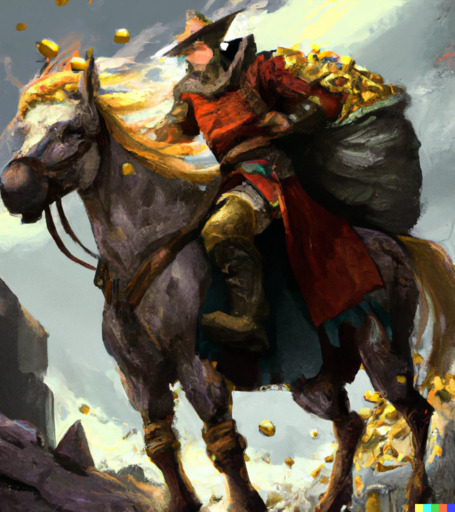
\includegraphics[width=\columnwidth]{equipment/tools goods and mounts}

        The world of Rise has a wide range of minor items like backpacks, blankets, and ten-foot poles.
        In general, the cost of those items is so insignificant from the perspective of an adventuring party that it's not worth the effort to track their cost in detail.
        A subset of particularly expensive items is included in \tref{Permanent Tools, Goods, and Mounts}.

        \subsection{Standard Adventuring Kit}\label{Standard Adventuring Kit}
          % Technically 15.2 gp and 50.5 pounds
          A standard adventuring kit is a rank 0 item (1 gp), weighs 50 pounds, and contains the following items:
          \begin{raggeditemize}
            \item Backpack
            \item Bedroll
            \item Flint and steel
            \item Rations, trail (8 days)
            \item Rope, hempen (60 ft.)
            \item Sack (empty)
            \item Tent
            \item Torch
            \item Waterskin
          \end{raggeditemize}
      \end{longtablepreface}

      \input{generated/permanent_tools_table.tex}
  \end{longcolumn}

  \input{generated/permanent_tools.tex}

  % Magic consumables are a loosely limited slot, but being consumable is a big downside.
  % They have the same power level as spells.
  \begin{longcolumn}
    \section{Consumables}\label{Consumables}

      \subsection{Potions}
        A potion is a magical liquid that is typically contained in a Fine vial.
        Drinking a potion, or administering a potion to an unconscious creature, requires a standard action.
        Potions cannot be safely mixed together without diluting their magic, so you cannot consume two potions with the same action.

        \input{generated/consumable_tools_table.tex}
  \end{longcolumn}

  \input{generated/consumable_tools.tex}

% Magic weapons are a highly limited slot.
% They have the same power level as self-attune spells.
\begin{longcolumn}
    \section{Magic Weapons}\label{Magic Weapons}
    \begin{longtablepreface}

      Magic weapons improve a character's combat abilities.
      They must be wielded to gain their effects.

      \parhead{Ranged Weapons and Ammunition} Any magical properties of a \weapontag{Projectile} weapon also apply to all ammunition fired from that weapon.

      \parhead{Craft Skills} The craft skills used to create and repair items are listed in parentheses before the item's description.
      All magic weapons simply use the same materials as the original, nonmagical weapon.

      \parhead{Property Limits} Normally, a weapon can only have one magic item property.
      \weapontag{Heavy} items can have two magic item properties instead of one.
    \end{longtablepreface}

    \input{generated/magic_weapons_table.tex}

\end{longcolumn}

\input{generated/magic_weapons.tex}

% Magic armor is a highly limited slot.
% They have the same power level as self-attune spells.
\begin{longcolumn}
  \section{Magic Armor}\label{Magic Armor}
    \begin{longtablepreface}
      Magic body armor must be worn to gain its effects, while magic shields must be wielded.
      You cannot imbue magic body armor effects on ordinary clothing, even if that clothing is worn on the body instead of armor.

      \parhead{Property Limits} A suit of body armor can only have one magic item property.
      A shield can also have one magic item property.
    \end{longtablepreface}

    \input{generated/magic_armor_table.tex}

\end{longcolumn}

\input{generated/magic_armor.tex}

% Magic apparel is a loosely limited slot.
% They are one rank behind self-attune spells.
\begin{longcolumn}
  \section{Magic Apparel}
    \begin{longtablepreface}
      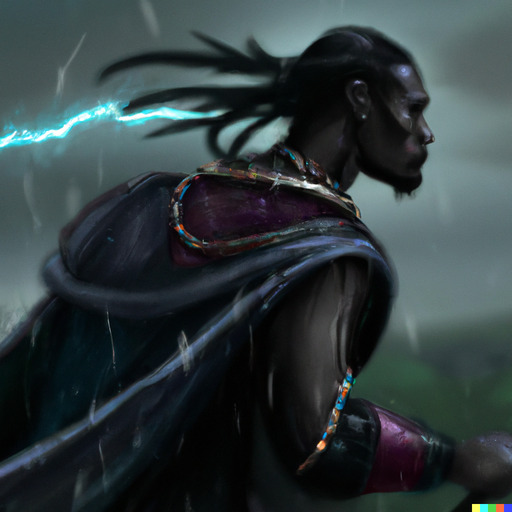
\includegraphics[width=\columnwidth]{equipment/magic apparel}
      Magic apparel items must be worn to gain their effects.

      \subsection{Body Slots}\label{Body Slots}
        The main limiting factor on how many items you can have equipped is your attunement points, not the physical location of your items on your body.
        However, there are limits to how many items you can wear of the same type, as described below.
        For item types not listed here, use reasonable judgment about what would be plausible.
        \begin{raggeditemize}
          \item Amulet: Up to 2
          \item Belt: Up to 2
          \item Boots: Up to 1
          \item Circlet: Up to 2
          \item Cloak: Up to 2
          \item Gauntlets: Up to 1 (separate from gloves)
          \item Gloves: Up to 1 (separate from gauntlets)
          \item Rings: Up to 5 per hand
          \item Tattoo: Any number, but only 1 per specific tattoo location
        \end{raggeditemize}

      \parhead{Property Limits} An apparel item can only have one magic item property.
    \end{longtablepreface}

    
\begin{longtablewrapper}
\begin{longtable}{p{15em} p{3em} p{6em} p{25em} p{3em}}

\lcaption{Apparel Items} \\
\tb{Name} & \tb{Level} & \tb{Typical Price} & \tb{Description} & \tb{Page} \tableheaderrule
Bracers of Archery & \nth{1} & 50 gp & Grants bow proficiency & \pageref{item:Bracers of Archery} \\
Belt of Healing & \nth{2} & 125 gp & Grants healing & \pageref{item:Belt of Healing} \\
Boots of the Winterlands & \nth{2} & 125 gp & Eases travel in cold areas & \pageref{item:Boots of the Winterlands} \\
Bracers of Armor & \nth{2} & 125 gp & Grants invisible armor & \pageref{item:Bracers of Armor} \\
Gauntlets of Improvisation & \nth{2} & 125 gp & Grants \plus1d damage with improvised weapons & \pageref{item:Gauntlets of Improvisation} \\
Ring of Elemental Endurance & \nth{2} & 125 gp & Grants tolerance of temperature extremes & \pageref{item:Ring of Elemental Endurance} \\
Shield of Bashing & \nth{2} & 125 gp & Grants \plus2 power & \pageref{item:Shield of Bashing} \\
Torchlight Gloves & \nth{2} & 125 gp & Sheds light as a torch & \pageref{item:Torchlight Gloves} \\
Ocular Circlet & \nth{3} & 250 gp & Can allow you to see at a distance & \pageref{item:Ocular Circlet} \\
Ring of Nourishment & \nth{3} & 250 gp & Provides food and water & \pageref{item:Ring of Nourishment} \\
Boots of Earth's Embrace & \nth{4} & 500 gp & Grants immunity to forced movement & \pageref{item:Boots of Earth's Embrace} \\
Boots of Elvenkind & \nth{4} & 500 gp & Grants \plus2 Stealth & \pageref{item:Boots of Elvenkind} \\
Circlet of Persuasion & \nth{4} & 500 gp & Grants \plus2 Persuasion & \pageref{item:Circlet of Persuasion} \\
Gauntlet of the Ram & \nth{4} & 500 gp & Knocks back foe when used to strike & \pageref{item:Gauntlet of the Ram} \\
Mask of Water Breathing & \nth{4} & 500 gp & Allows breathing water like air & \pageref{item:Mask of Water Breathing} \\
Throwing Gloves & \nth{4} & 500 gp & Allows throwing any item accurately & \pageref{item:Throwing Gloves} \\
Acid Coated & \nth{5} & 800 gp & Deals acid damage to anything it touches & \pageref{item:Acid Coated} \\
Amulet of Translocation & \nth{5} & 800 gp & Grants ability to teleport up to 30 feet & \pageref{item:Amulet of Translocation} \\
Circlet of Blasting & \nth{5} & 800 gp & Can blast foe with fire & \pageref{item:Circlet of Blasting} \\
Hidden Armor & \nth{5} & 800 gp & Can look like normal clothing & \pageref{item:Hidden Armor} \\
Protective Armor & \nth{5} & 800 gp & Grants \plus1 Armor defense & \pageref{item:Protective Armor} \\
Protective Shield & \nth{5} & 800 gp & Grants \plus1 Armor defense & \pageref{item:Protective Shield} \\
Shield of Arrow Catching & \nth{5} & 800 gp & Redirects small nearby projectiles to hit you & \pageref{item:Shield of Arrow Catching} \\
Shield of Arrow Deflection & \nth{5} & 800 gp & Blocks small projectiles & \pageref{item:Shield of Arrow Deflection} \\
Translocation & \nth{5} & 800 gp & Grants ability to teleport up to 30 feet & \pageref{item:Translocation} \\
Agile & \nth{6} & 1,200 gp & Grants \plus2 Reflex defense & \pageref{item:Agile} \\
Amulet of Health & \nth{6} & 1,200 gp & Grants 2 additional hit points & \pageref{item:Amulet of Health} \\
Amulet of Nondetection & \nth{6} & 1,200 gp & Grants \plus4 to defenses against detection & \pageref{item:Amulet of Nondetection} \\
Boots of Speed & \nth{6} & 1,200 gp & Increases speed by ten feet & \pageref{item:Boots of Speed} \\
Featherlight Armor & \nth{6} & 1,200 gp & Reduces encumbrance by 1 & \pageref{item:Featherlight Armor} \\
Fortified & \nth{6} & 1,200 gp & Grants \plus2 Fortitude defense & \pageref{item:Fortified} \\
Quilled Cloak & \nth{6} & 1,200 gp & Deals damage to creatures that grapple you & \pageref{item:Quilled Cloak} \\
Willguard & \nth{6} & 1,200 gp & Grants \plus2 Mental defense & \pageref{item:Willguard} \\
Anchoring & \nth{7} & 1,800 gp & Protects you from most forced movement attacks & \pageref{item:Anchoring} \\
Armor of Fortification & \nth{7} & 1,800 gp & Reduces critical hits from strikes & \pageref{item:Armor of Fortification} \\
Boots of Water Walking & \nth{7} & 1,800 gp & Allows walking on liquids & \pageref{item:Boots of Water Walking} \\
Boots of the Skydancer & \nth{7} & 1,800 gp & Can walk on air & \pageref{item:Boots of the Skydancer} \\
Bracers of Archery, Greater & \nth{7} & 1,800 gp & Grants bow proficiency, \plus1 ranged accuracy & \pageref{item:Bracers of Archery, Greater} \\
Bracers of Repulsion & \nth{7} & 1,800 gp & Can knock nearby creatures back & \pageref{item:Bracers of Repulsion} \\
Crown of Lightning & \nth{7} & 1,800 gp & Continuously damages nearby enemies & \pageref{item:Crown of Lightning} \\
Gauntlet of the Ram, Greater & \nth{7} & 1,800 gp & Knocks back foe farther when use to strike & \pageref{item:Gauntlet of the Ram, Greater} \\
Gauntlets of Improvisation, Greater & \nth{7} & 1,800 gp & Grants \plus2d damage with improvised weapons & \pageref{item:Gauntlets of Improvisation, Greater} \\
Gloves of Spell Investment & \nth{7} & 1,800 gp & Can invest a spell to cast later & \pageref{item:Gloves of Spell Investment} \\
Hexward Amulet & \nth{7} & 1,800 gp & Grants \plus1 defenses against targeted magical attacks & \pageref{item:Hexward Amulet} \\
Lifekeeping Belt & \nth{7} & 1,800 gp & Grants \plus1 bonus to \glossterm{vital rolls} & \pageref{item:Lifekeeping Belt} \\
Ring of Sustenance & \nth{7} & 1,800 gp & Provides food, water, and rest & \pageref{item:Ring of Sustenance} \\
Amulet of Mighty Fists & \nth{8} & 2,750 gp & Grants \plus2 power with natural and unarmed attacks & \pageref{item:Amulet of Mighty Fists} \\
Armor of Energy Resistance & \nth{8} & 2,750 gp & Reduces energy damage & \pageref{item:Armor of Energy Resistance} \\
Armor of Invulnerability & \nth{8} & 2,750 gp & Reduces physical damage & \pageref{item:Armor of Invulnerability} \\
Assassin's Cloak & \nth{8} & 2,750 gp & Grants invisibility while inactive & \pageref{item:Assassin's Cloak} \\
Avian Cloak & \nth{8} & 2,750 gp & Grants a glide speed & \pageref{item:Avian Cloak} \\
Belt of Healing, Greater & \nth{8} & 2,750 gp & Grants more healing & \pageref{item:Belt of Healing, Greater} \\
Boots of Gravitation & \nth{8} & 2,750 gp & Redirects personal gravity & \pageref{item:Boots of Gravitation} \\
Cloak of Mist & \nth{8} & 2,750 gp & Fills nearby area with fog & \pageref{item:Cloak of Mist} \\
Ring of Protection & \nth{8} & 2,750 gp & Grants \plus1 to Armor and Reflex defenses & \pageref{item:Ring of Protection} \\
Shield of Boulder Catching & \nth{8} & 2,750 gp & Redirects large nearby projectiles to hit you & \pageref{item:Shield of Boulder Catching} \\
Shield of Boulder Deflection & \nth{8} & 2,750 gp & Can block large projectiles & \pageref{item:Shield of Boulder Deflection} \\
Crown of Flame & \nth{9} & 4,000 gp & Grants nearby allies immunity to fire damage & \pageref{item:Crown of Flame} \\
Greatreach Bracers & \nth{9} & 4,000 gp & Increases reach by five feet & \pageref{item:Greatreach Bracers} \\
Hidden Armor, Greater & \nth{9} & 4,000 gp & Can look and sound like normal clothing & \pageref{item:Hidden Armor, Greater} \\
Mask of Air & \nth{9} & 4,000 gp & Allows breathing in any environment & \pageref{item:Mask of Air} \\
Ocular Circlet, Greater & \nth{9} & 4,000 gp & Can allow you to see at a greater distance & \pageref{item:Ocular Circlet, Greater} \\
Ring of Angel's Grace & \nth{9} & 4,000 gp & Grants \plus2 Mental and slows falls & \pageref{item:Ring of Angel's Grace} \\
Boots of Speed, Greater & \nth{10} & 6,500 gp & Increases speed by twenty feet & \pageref{item:Boots of Speed, Greater} \\
Circlet of Blasting, Greater & \nth{10} & 6,500 gp & Can blast foe with intense fire & \pageref{item:Circlet of Blasting, Greater} \\
Crater Boots & \nth{10} & 6,500 gp & Deals your falling damage to enemies & \pageref{item:Crater Boots} \\
Titan Gauntlets & \nth{10} & 6,500 gp & Grants \plus2 \glossterm{mundane} power & \pageref{item:Titan Gauntlets} \\
Winged Boots & \nth{10} & 6,500 gp & Grants limited flight & \pageref{item:Winged Boots} \\
Amulet of Translocation, Greater & \nth{11} & 10,000 gp & Grants ability to teleport up to 100 feet & \pageref{item:Amulet of Translocation, Greater} \\
Crown of Thunder & \nth{11} & 10,000 gp & Continously deafens nearby enemies & \pageref{item:Crown of Thunder} \\
Shield of Arrow Catching, Greater & \nth{11} & 10,000 gp & Selectively redirects small nearby projectiles to hit you & \pageref{item:Shield of Arrow Catching, Greater} \\
Shield of Bashing, Greater & \nth{11} & 10,000 gp & Grants \plus4 power & \pageref{item:Shield of Bashing, Greater} \\
Translocation, Greater & \nth{11} & 10,000 gp & Grants ability to teleport up to 100 feet & \pageref{item:Translocation, Greater} \\
Amulet of the Planes & \nth{12} & 16,000 gp & Aids travel with \ritual{plane shift} & \pageref{item:Amulet of the Planes} \\
Armor of Fortification, Mystic & \nth{12} & 16,000 gp & Reduces critical hits from all attacks & \pageref{item:Armor of Fortification, Mystic} \\
Boots of Freedom & \nth{12} & 16,000 gp & Grants immunity to almost all mobility restrictions & \pageref{item:Boots of Freedom} \\
Featherlight Armor, Greater & \nth{12} & 16,000 gp & Reduces encumbrance by 2 & \pageref{item:Featherlight Armor, Greater} \\
Greater Quilled Cloak & \nth{12} & 16,000 gp & Deals more damage to creatures that grapple you & \pageref{item:Greater Quilled Cloak} \\
Ring of Energy Resistance & \nth{12} & 16,000 gp & Reduces energy damage & \pageref{item:Ring of Energy Resistance} \\
Seven League Boots & \nth{12} & 16,000 gp & Teleport seven leages with a step & \pageref{item:Seven League Boots} \\
Shield of Mystic Reflection & \nth{12} & 16,000 gp & React to reflect magical attacks & \pageref{item:Shield of Mystic Reflection} \\
Anchoring, Greater & \nth{13} & 25,000 gp & Protects you from all forced movement and teleportation attacks & \pageref{item:Anchoring, Greater} \\
Assassin's Cloak, Greater & \nth{13} & 25,000 gp & Grants longer invisibility while inactive & \pageref{item:Assassin's Cloak, Greater} \\
Boots of the Skydancer, Greater & \nth{13} & 25,000 gp & description & \pageref{item:Boots of the Skydancer, Greater} \\
Crown of Frost & \nth{13} & 25,000 gp & Continuously damages nearby enemies & \pageref{item:Crown of Frost} \\
Gloves of Spell Investment, Greater & \nth{13} & 25,000 gp & Can invest two spells to cast later & \pageref{item:Gloves of Spell Investment, Greater} \\
Hexproof Amulet, Greater & \nth{13} & 25,000 gp & Grants \plus2 defenses against targeted magical attacks & \pageref{item:Hexproof Amulet, Greater} \\
Lifekeeping Belt, Greater & \nth{13} & 25,000 gp & Grants \plus2 bonus to \glossterm{vital rolls} & \pageref{item:Lifekeeping Belt, Greater} \\
Vanishing Cloak & \nth{13} & 25,000 gp & Can teleport a short distance and grant invisibility & \pageref{item:Vanishing Cloak} \\
Amulet of Nondetection, Greater & \nth{14} & 37,000 gp & Grants \plus8 to defenses against detection & \pageref{item:Amulet of Nondetection, Greater} \\
Armor of Energy Resistance, Greater & \nth{14} & 37,000 gp & Significantly reduces energy damage & \pageref{item:Armor of Energy Resistance, Greater} \\
Armor of Invulnerability & \nth{14} & 37,000 gp & Significantly reduces physical damage & \pageref{item:Armor of Invulnerability} \\
Belt of Healing, Supreme & \nth{14} & 37,000 gp & Grants more healing & \pageref{item:Belt of Healing, Supreme} \\
Boots of Speed, Supreme & \nth{14} & 37,000 gp & Increases speed by thirty feet & \pageref{item:Boots of Speed, Supreme} \\
Protective Armor, Greater & \nth{14} & 37,000 gp & Grants \plus2 Armor defense & \pageref{item:Protective Armor, Greater} \\
Protective Shield, Greater & \nth{14} & 37,000 gp & Grants \plus2 Armor defense & \pageref{item:Protective Shield, Greater} \\
Shield of Arrow Deflection, Greater & \nth{14} & 37,000 gp & Blocks small projectiles & \pageref{item:Shield of Arrow Deflection, Greater} \\
Agile, Greater & \nth{15} & 55,000 gp & Grants \plus4 Reflex defense & \pageref{item:Agile, Greater} \\
Amulet of Health, Greater & \nth{15} & 55,000 gp & Grants 4 additional hit points & \pageref{item:Amulet of Health, Greater} \\
Armor of Fortification, Greater & \nth{15} & 55,000 gp & Drastically reduces critical hits from strikes & \pageref{item:Armor of Fortification, Greater} \\
Bracers of Repulsion, Greater & \nth{15} & 55,000 gp & Can knock many nearby creatures back & \pageref{item:Bracers of Repulsion, Greater} \\
Fortified, Greater & \nth{15} & 55,000 gp & Grants \plus4 Fortitude defense & \pageref{item:Fortified, Greater} \\
Ring of Regeneration & \nth{15} & 55,000 gp & Automatically removes vital wounds & \pageref{item:Ring of Regeneration} \\
Willguard, Greater & \nth{15} & 55,000 gp & Grants \plus4 Mental defense & \pageref{item:Willguard, Greater} \\
Amulet of Mighty Fists, Greater & \nth{16} & 85,000 gp & Grants \plus4 power with natural and unarmed attacks & \pageref{item:Amulet of Mighty Fists, Greater} \\
Astral Boots & \nth{16} & 85,000 gp & Allows teleporting instead of moving & \pageref{item:Astral Boots} \\
Circlet of Blasting, Supreme & \nth{16} & 85,000 gp & Can blast foe with supremely intense fire & \pageref{item:Circlet of Blasting, Supreme} \\
Cloak of Mist, Greater & \nth{16} & 85,000 gp & Fills nearby area with thick fog & \pageref{item:Cloak of Mist, Greater} \\
Ring of Protection, Greater & \nth{16} & 85,000 gp & Grants \plus2 to Armor and Reflex defenses & \pageref{item:Ring of Protection, Greater} \\
Amulet of Translocation, Supreme & \nth{17} & 125,000 gp & Grants ability to teleport up to 300 feet & \pageref{item:Amulet of Translocation, Supreme} \\
Greatreach Bracers, Greater & \nth{17} & 125,000 gp & Increases reach by ten feet & \pageref{item:Greatreach Bracers, Greater} \\
Shield of Boulder Deflection, Greater & \nth{17} & 125,000 gp & Blocks large projectiles & \pageref{item:Shield of Boulder Deflection, Greater} \\
Translocation, Supreme & \nth{17} & 125,000 gp & Grants ability to teleport up to 300 feet & \pageref{item:Translocation, Supreme} \\
Featherlight Armor, Supreme & \nth{18} & 190,000 gp & Reduces encumbrance by 2 & \pageref{item:Featherlight Armor, Supreme} \\
Supreme Quilled Cloak & \nth{18} & 190,000 gp & Deals even more damage to creatures that grapple you & \pageref{item:Supreme Quilled Cloak} \\
Hexproof Amulet, Supreme & \nth{19} & 280,000 gp & Grants \plus3 defenses against targeted magical attacks & \pageref{item:Hexproof Amulet, Supreme} \\
Lifekeeping Belt, Supreme & \nth{19} & 280,000 gp & Grants \plus3 bonus to \glossterm{vital rolls} & \pageref{item:Lifekeeping Belt, Supreme} \\
Titan Gauntlets, Greater & \nth{19} & 280,000 gp & Grants \plus4 \glossterm{mundane} power & \pageref{item:Titan Gauntlets, Greater} \\
Armor of Energy Resistance, Supreme & \nth{20} & 400,000 gp & Drastically reduces energy damage & \pageref{item:Armor of Energy Resistance, Supreme} \\
Armor of Invulnerability, Greater & \nth{20} & 400,000 gp & Drastically reduces physical damage & \pageref{item:Armor of Invulnerability, Greater} \\
Shield of Bashing, Supreme & \nth{20} & 400,000 gp & Grants \plus6 power & \pageref{item:Shield of Bashing, Supreme} \\

\end{longtable}
\end{longtablewrapper}


\end{longcolumn}

\lowercase{\hypertarget{item:Amulet of Mighty Fists}{}}\label{item:Amulet of Mighty Fists}
\hypertarget{item:Amulet of Mighty Fists}{\subsubsection{Amulet of Mighty Fists\hfill\nth{6}}}
You gain a \plus1d bonus to \glossterm{strike damage} with \glossterm{unarmed attacks} and natural weapons.
\parhead*{Tags} \glossterm{Enhancement}
\parhead*{Materials} Jewelry
\lowercase{\hypertarget{item:Amulet of Mighty Fists, Greater}{}}\label{item:Amulet of Mighty Fists, Greater}
\hypertarget{item:Amulet of Mighty Fists, Greater}{\subsubsection{Amulet of Mighty Fists, Greater\hfill\nth{14}}}
You gain a \plus2d bonus to \glossterm{strike damage} with \glossterm{unarmed attacks} and natural weapons.
\parhead*{Tags} \glossterm{Enhancement}
\parhead*{Materials} Jewelry
\lowercase{\hypertarget{item:Armor of Energy Resistance}{}}\label{item:Armor of Energy Resistance}
\hypertarget{item:Armor of Energy Resistance}{\subsubsection{Armor of Energy Resistance\hfill\nth{4}}}
You have \glossterm{damage reduction} equal to the item's \glossterm{power} against \glossterm{energy damage}.
Whenever you resist energy with this item, it sheds light as a torch until the end of the next round.
The color of the light depends on the energy damage resisted: blue for cold, yellow for electricity, red for fire, and brown for sonic.
\parhead*{Tags} \glossterm{Shielding}
\parhead*{Materials} Bone, metal
\lowercase{\hypertarget{item:Armor of Energy Resistance, Greater}{}}\label{item:Armor of Energy Resistance, Greater}
\hypertarget{item:Armor of Energy Resistance, Greater}{\subsubsection{Armor of Energy Resistance, Greater\hfill\nth{12}}}
This item functions like the \mitem{armor of energy resistance} item, except that the damage reduction is equal to twice the item's \glossterm{power}.
\parhead*{Tags} \glossterm{Shielding}
\parhead*{Materials} Bone, metal
\lowercase{\hypertarget{item:Armor of Fortification}{}}\label{item:Armor of Fortification}
\hypertarget{item:Armor of Fortification}{\subsubsection{Armor of Fortification\hfill\nth{7}}}
You gain a \plus5 bonus to defenses when determining whether a \glossterm{strike} gets a \glossterm{critical hit} against you instead of a normal hit.
\parhead*{Tags} \glossterm{Imbuement}
\parhead*{Materials} Bone, metal
\lowercase{\hypertarget{item:Armor of Fortification, Greater}{}}\label{item:Armor of Fortification, Greater}
\hypertarget{item:Armor of Fortification, Greater}{\subsubsection{Armor of Fortification, Greater\hfill\nth{15}}}
This item functions like the \mitem{armor of fortification} item, except that the bonus increases to \plus10.
\parhead*{Tags} \glossterm{Imbuement}
\parhead*{Materials} Bone, metal
\lowercase{\hypertarget{item:Armor of Fortification, Mystic}{}}\label{item:Armor of Fortification, Mystic}
\hypertarget{item:Armor of Fortification, Mystic}{\subsubsection{Armor of Fortification, Mystic\hfill\nth{12}}}
This item functions like the \mitem{armor of fortification} item, except that it applies against all attacks instead of only against; \glossterm{strikes}.
\parhead*{Tags} \glossterm{Imbuement}
\parhead*{Materials} Bone, metal
\lowercase{\hypertarget{item:Armor of Invulnerability}{}}\label{item:Armor of Invulnerability}
\hypertarget{item:Armor of Invulnerability}{\subsubsection{Armor of Invulnerability\hfill\nth{8}}}
You have \glossterm{damage reduction} equal to this item's \glossterm{power} against damage from \glossterm{physical attacks}.
\parhead*{Tags} \glossterm{Shielding}
\parhead*{Materials} Bone, metal
\lowercase{\hypertarget{item:Armor of Invulnerability, Greater}{}}\label{item:Armor of Invulnerability, Greater}
\hypertarget{item:Armor of Invulnerability, Greater}{\subsubsection{Armor of Invulnerability, Greater\hfill\nth{16}}}
This item functions like the \mitem{armor of invulnerability} item, except that the damage reduction is equal to twice the item's \glossterm{power}.
You have \glossterm{damage reduction} equal to the item's \glossterm{power} against damage from \glossterm{physical attacks}.
\parhead*{Tags} \glossterm{Shielding}
\parhead*{Materials} Bone, metal
\lowercase{\hypertarget{item:Armor of Magic Resistance}{}}\label{item:Armor of Magic Resistance}
\hypertarget{item:Armor of Magic Resistance}{\subsubsection{Armor of Magic Resistance\hfill\nth{14}}}
You have \glossterm{magic resistance} equal to 5 + the item's \glossterm{power}.
\parhead*{Tags} \glossterm{Shielding}
\parhead*{Materials} Bone, metal
\lowercase{\hypertarget{item:Assassin's Cloak}{}}\label{item:Assassin's Cloak}
\hypertarget{item:Assassin's Cloak}{\subsubsection{Assassin's Cloak\hfill\nth{7}}}
At the end of each round, if you took no actions that round, you become \glossterm{invisible} until the end of the next round.
\parhead*{Tags} \glossterm{Glamer}
\parhead*{Materials} Textiles
\lowercase{\hypertarget{item:Assassin's Cloak, Greater}{}}\label{item:Assassin's Cloak, Greater}
\hypertarget{item:Assassin's Cloak, Greater}{\subsubsection{Assassin's Cloak, Greater\hfill\nth{17}}}
At the end of each round, if you did not attack a creature that round, you become \glossterm{invisible} until the end of the next round.
\parhead*{Tags} \glossterm{Glamer}
\parhead*{Materials} Textiles
\lowercase{\hypertarget{item:Astral Boots}{}}\label{item:Astral Boots}
\hypertarget{item:Astral Boots}{\subsubsection{Astral Boots\hfill\nth{16}}}
Whenever you move, you can teleport the same distance instead.
This does not change the total distance you can move, but you can teleport in any direction, even vertically.
You cannot teleport to locations you do not have \glossterm{line of sight} and \glossterm{line of effect} to.
\parhead*{Tags} \glossterm{Teleportation}
\parhead*{Materials} Bone, leather, metal
\lowercase{\hypertarget{item:Belt of Healing}{}}\label{item:Belt of Healing}
\hypertarget{item:Belt of Healing}{\subsubsection{Belt of Healing\hfill\nth{1}}}
When you use the \textit{recover} action, you heal \plus1d hit points.
\parhead*{Tags} \glossterm{Life}
\parhead*{Materials} Leather, textiles
\lowercase{\hypertarget{item:Belt of Healing, Greater}{}}\label{item:Belt of Healing, Greater}
\hypertarget{item:Belt of Healing, Greater}{\subsubsection{Belt of Healing, Greater\hfill\nth{8}}}
When you use the \textit{recover} action, you heal \plus2d hit points.
\parhead*{Tags} \glossterm{Life}
\parhead*{Materials} Leather, textiles
\lowercase{\hypertarget{item:Belt of Heroic Recovery}{}}\label{item:Belt of Heroic Recovery}
\hypertarget{item:Belt of Heroic Recovery}{\subsubsection{Belt of Heroic Recovery\hfill\nth{6}}}
% TODO: timing?
As an \glossterm{immediate action} when you get a \glossterm{critical hit}, you can take the \textit{recover} action.
\parhead*{Tags} \glossterm{Life}
\parhead*{Materials} Leather, textiles
\lowercase{\hypertarget{item:Boots of Earth's Embrace}{}}\label{item:Boots of Earth's Embrace}
\hypertarget{item:Boots of Earth's Embrace}{\subsubsection{Boots of Earth's Embrace\hfill\nth{4}}}
While you are standing on solid ground, you are immune to effects that would force you to move.
This does not protect you from other effects of those attacks, such as damage.
\parhead*{Tags} \glossterm{Earth}, \glossterm{Enhancement}
\parhead*{Materials} Bone, leather, metal
\lowercase{\hypertarget{item:Boots of Freedom}{}}\label{item:Boots of Freedom}
\hypertarget{item:Boots of Freedom}{\subsubsection{Boots of Freedom\hfill\nth{6}}}
You are immune to effects that restrict your mobility.
This removes all penalties you would suffer for acting underwater, except for those relating to using ranged weapons.
This does not prevent you from being \grappled, but you gain a \plus10 bonus to your defense against \glossterm{grapple} attacks.
\parhead*{Tags} \glossterm{Imbuement}
\parhead*{Materials} Bone, leather, metal
\lowercase{\hypertarget{item:Boots of Freedom, Greater}{}}\label{item:Boots of Freedom, Greater}
\hypertarget{item:Boots of Freedom, Greater}{\subsubsection{Boots of Freedom, Greater\hfill\nth{12}}}
These boots function like \mitem{boots of freedom}, except that you are also immune to being \grappled.
\parhead*{Tags} \glossterm{Imbuement}
\parhead*{Materials} Bone, leather, metal
\lowercase{\hypertarget{item:Boots of Gravitation}{}}\label{item:Boots of Gravitation}
\hypertarget{item:Boots of Gravitation}{\subsubsection{Boots of Gravitation\hfill\nth{8}}}
While these boots are within 5 feet of a solid surface, gravity pulls you towards the solid surface closest to your boots rather than in the normal direction.
This can allow you to walk easily on walls or even ceilings.
\parhead*{Tags} \glossterm{Imbuement}
\parhead*{Materials} Bone, leather, metal
\lowercase{\hypertarget{item:Boots of Speed}{}}\label{item:Boots of Speed}
\hypertarget{item:Boots of Speed}{\subsubsection{Boots of Speed\hfill\nth{5}}}
You gain a \plus10 foot bonus to your speed in all your movement modes, up to a maximum of double your normal speed.
\parhead*{Tags} \glossterm{Temporal}
\parhead*{Materials} Bone, leather, metal
\lowercase{\hypertarget{item:Boots of Speed, Greater}{}}\label{item:Boots of Speed, Greater}
\hypertarget{item:Boots of Speed, Greater}{\subsubsection{Boots of Speed, Greater\hfill\nth{13}}}
You gain a \plus30 foot bonus to your speed in all your movement modes, up to a maximum of double your normal speed.
\parhead*{Tags} \glossterm{Temporal}
\parhead*{Materials} Bone, leather, metal
\lowercase{\hypertarget{item:Boots of Water Walking}{}}\label{item:Boots of Water Walking}
\hypertarget{item:Boots of Water Walking}{\subsubsection{Boots of Water Walking\hfill\nth{7}}}
You treat the surface of all liquids as if they were firm ground.
Your feet hover about an inch above the liquid's surface, allowing you to traverse dangerous liquids without harm as long as the surface is calm.
If you are below the surface of the liquid, you rise towards the surface at a rate of 60 feet per round.
Thick liquids, such as mud and lava, may cause you to rise more slowly.
\parhead*{Tags} \glossterm{Imbuement}
\parhead*{Materials} Bone, leather, metal
\lowercase{\hypertarget{item:Boots of the Winterlands}{}}\label{item:Boots of the Winterlands}
\hypertarget{item:Boots of the Winterlands}{\subsubsection{Boots of the Winterlands\hfill\nth{2}}}
You can travel across snow and ice without slipping or suffering movement penalties for the terrain.
% TODO: degree symbol?
In addition, the boots keep you warn, protecting you in environments as cold as \minus50 Fahrenheit.
\parhead*{Tags} \glossterm{Enhancement}
\parhead*{Materials} Bone, leather, metal
\lowercase{\hypertarget{item:Bracers of Archery}{}}\label{item:Bracers of Archery}
\hypertarget{item:Bracers of Archery}{\subsubsection{Bracers of Archery\hfill\nth{1}}}
You are proficient with bows.
\parhead*{Tags} \glossterm{Enhancement}
\parhead*{Materials} Bone, leather, metal, wood
\lowercase{\hypertarget{item:Bracers of Armor}{}}\label{item:Bracers of Armor}
\hypertarget{item:Bracers of Armor}{\subsubsection{Bracers of Armor\hfill\nth{2}}}
You gain a \plus2 bonus to Armor defense.
The protection from these bracers is treated as body armor, and it does not stack with any other body armor you wear.
\parhead*{Tags} \glossterm{Shielding}
\parhead*{Materials} Bone, leather, metal, wood
\lowercase{\hypertarget{item:Bracers of Repulsion}{}}\label{item:Bracers of Repulsion}
\hypertarget{item:Bracers of Repulsion}{\subsubsection{Bracers of Repulsion\hfill\nth{4}}}
Whenever a creature hits you with a melee \glossterm{strike} during the \glossterm{action phase},
you can spend an \glossterm{action point} to use this item as an \glossterm{immediate action}.
If you do, you make a \glossterm{shove} attack against that creature during the \glossterm{delayed action phase}, using this item's power in place of your Strength.
\parhead*{Tags} \glossterm{Telekinesis}
\parhead*{Materials} Bone, leather, metal, wood
\lowercase{\hypertarget{item:Bracers of Repulsion, Greater}{}}\label{item:Bracers of Repulsion, Greater}
\hypertarget{item:Bracers of Repulsion, Greater}{\subsubsection{Bracers of Repulsion, Greater\hfill\nth{11}}}
This item functions like the \mitem{bracers of repulsion} item, except that it does not cost an action point to use.
\parhead*{Tags} \glossterm{Telekinesis}
\parhead*{Materials} Bone, leather, metal, wood
\lowercase{\hypertarget{item:Cloak of Mist}{}}\label{item:Cloak of Mist}
\hypertarget{item:Cloak of Mist}{\subsubsection{Cloak of Mist\hfill\nth{8}}}
Fog constantly fills an \areamed radius emanation from you.
This fog does not fully block sight, but it provides \concealment.
If a 5-foot square of fog takes fire damage equal to half this item's \glossterm{power}, the fog disappears from that area until the end of the next round.
\parhead*{Tags} \glossterm{Fog}, \glossterm{Manifestation}
\parhead*{Materials} Textiles
\lowercase{\hypertarget{item:Cloak of Mist, Greater}{}}\label{item:Cloak of Mist, Greater}
\hypertarget{item:Cloak of Mist, Greater}{\subsubsection{Cloak of Mist, Greater\hfill\nth{16}}}
A thick fog constantly fills an \areamed radius emanation from you.
This fog completely blocks sight beyond 10 feet.
Within that range, it still provides \concealment.
If a 5-foot square of fog takes fire damage equal to this item's \glossterm{power}, the fog disappears from that area until the end of the next round.
\parhead*{Tags} \glossterm{Fog}, \glossterm{Manifestation}
\parhead*{Materials} Textiles
\lowercase{\hypertarget{item:Crown of Flame}{}}\label{item:Crown of Flame}
\hypertarget{item:Crown of Flame}{\subsubsection{Crown of Flame\hfill\nth{5}}}
This crown is continuously on fire.
The flame sheds light as a torch.
You and all allies within an \arealarge radius emanation from you are immune to fire damage.
\parhead*{Tags} \glossterm{Fire}
\parhead*{Materials} Bone, metal
\lowercase{\hypertarget{item:Crown of Frost}{}}\label{item:Crown of Frost}
\hypertarget{item:Crown of Frost}{\subsubsection{Crown of Frost\hfill\nth{11}}}
At the end of each \glossterm{action phase}, you make a Power vs. Fortitude attack against all enemies within an \areamed radius emanation from you.
A hit deals cold \glossterm{standard damage} \minus3d.
Each creature that takes damage in this way is \fatigued until the end of the next round.
\parhead*{Tags} \glossterm{Cold}
\parhead*{Materials} Bone, metal
\lowercase{\hypertarget{item:Crown of Lightning}{}}\label{item:Crown of Lightning}
\hypertarget{item:Crown of Lightning}{\subsubsection{Crown of Lightning\hfill\nth{7}}}
This crown continuously crackles with electricity.
The constant sparks shed light as a torch.
At the end of each \glossterm{action phase}, you make a Power vs. Reflex attack against all enemies within an \areamed radius emanation from you.
A hit deals electricity \glossterm{standard damage} \minus3d.
\parhead*{Tags} \glossterm{Electricity}
\parhead*{Materials} Bone, metal
\lowercase{\hypertarget{item:Crown of Thunder}{}}\label{item:Crown of Thunder}
\hypertarget{item:Crown of Thunder}{\subsubsection{Crown of Thunder\hfill\nth{9}}}
The crown constantly emits a low-pitched rumbling.
To you and your allies, the sound is barely perceptible.
However, all enemies within an \arealarge radius emanation from you hear the sound as a deafening, continuous roll of thunder.
The noise blocks out all other sounds quieter than thunder, causing them to be \deafened while they remain in the area and until the end of the next round after they leave.
\parhead*{Tags} \glossterm{Sonic}
\parhead*{Materials} Bone, metal
\lowercase{\hypertarget{item:Featherlight Armor}{}}\label{item:Featherlight Armor}
\hypertarget{item:Featherlight Armor}{\subsubsection{Featherlight Armor\hfill\nth{4}}}
This armor's \glossterm{encumbrance penalty} is reduced by 2.
\parhead*{Tags} \glossterm{Enhancement}
\parhead*{Materials} Bone, metal
\lowercase{\hypertarget{item:Featherlight Armor, Greater}{}}\label{item:Featherlight Armor, Greater}
\hypertarget{item:Featherlight Armor, Greater}{\subsubsection{Featherlight Armor, Greater\hfill\nth{10}}}
This armor's \glossterm{encumbrance penalty} is reduced by 4.
\parhead*{Tags} \glossterm{Enhancement}
\parhead*{Materials} Bone, metal
\lowercase{\hypertarget{item:Gauntlet of the Ram}{}}\label{item:Gauntlet of the Ram}
\hypertarget{item:Gauntlet of the Ram}{\subsubsection{Gauntlet of the Ram\hfill\nth{2}}}
If you hit on a \glossterm{strike} with this gauntlet during the \glossterm{action phse}, you can attempt to \glossterm{shove} your foe during the \glossterm{delayed action phase}.
Making a strike with this gauntlet is equivalent to an \glossterm{unarmed attack}.
You do not need to move with your foe to push it back the full distance.
\parhead*{Tags} \glossterm{Telekinesis}
\parhead*{Materials} Bone, metal, wood
\lowercase{\hypertarget{item:Gauntlet of the Ram, Greater}{}}\label{item:Gauntlet of the Ram, Greater}
\hypertarget{item:Gauntlet of the Ram, Greater}{\subsubsection{Gauntlet of the Ram, Greater\hfill\nth{7}}}
This item functions like the \mitem{gauntlet of the ram}, except that you gain a bonus to the \glossterm{shove} attack equal to the damage you dealt with the \glossterm{strike}.
\parhead*{Tags} \glossterm{Telekinesis}
\parhead*{Materials} Bone, metal, wood
\lowercase{\hypertarget{item:Gauntlets of Improvisation}{}}\label{item:Gauntlets of Improvisation}
\hypertarget{item:Gauntlets of Improvisation}{\subsubsection{Gauntlets of Improvisation\hfill\nth{2}}}
You gain a \plus1d bonus to damage with \glossterm{improvised weapons}.
\parhead*{Tags} \glossterm{Enhancement}
\parhead*{Materials} Bone, metal, wood
\lowercase{\hypertarget{item:Gauntlets of Improvisation, Greater}{}}\label{item:Gauntlets of Improvisation, Greater}
\hypertarget{item:Gauntlets of Improvisation, Greater}{\subsubsection{Gauntlets of Improvisation, Greater\hfill\nth{7}}}
This item functions like the \mitem{gauntlets of improvisation}, except that the damage bonus is increased to \plus2d.
\parhead*{Tags} \glossterm{Enhancement}
\parhead*{Materials} Bone, metal, wood
\lowercase{\hypertarget{item:Greatreach Bracers}{}}\label{item:Greatreach Bracers}
\hypertarget{item:Greatreach Bracers}{\subsubsection{Greatreach Bracers\hfill\nth{9}}}
Your \glossterm{reach} is increased by 5 feet.
\parhead*{Tags} \glossterm{Imbuement}
\parhead*{Materials} Bone, leather, metal, wood
\lowercase{\hypertarget{item:Greatreach Bracers, Greater}{}}\label{item:Greatreach Bracers, Greater}
\hypertarget{item:Greatreach Bracers, Greater}{\subsubsection{Greatreach Bracers, Greater\hfill\nth{17}}}
Your \glossterm{reach} is increased by 10 feet.
\parhead*{Tags} \glossterm{Imbuement}
\parhead*{Materials} Bone, leather, metal, wood
\lowercase{\hypertarget{item:Hexproof Cloak}{}}\label{item:Hexproof Cloak}
\hypertarget{item:Hexproof Cloak}{\subsubsection{Hexproof Cloak\hfill\nth{18}}}
All \glossterm{magical} abilities that target you directly fail to affect you.
This does not protect you from abilities that affect an area.
\parhead*{Tags} \glossterm{Thaumaturgy}
\parhead*{Materials} Textiles
\lowercase{\hypertarget{item:Hexward Cloak}{}}\label{item:Hexward Cloak}
\hypertarget{item:Hexward Cloak}{\subsubsection{Hexward Cloak\hfill\nth{10}}}
You gain a \plus5 bonus to defenses against \glossterm{magical} abilities that target you directly.
This does not protect you from abilities that affect an area.
\parhead*{Tags} \glossterm{Thaumaturgy}
\parhead*{Materials} Textiles
\lowercase{\hypertarget{item:Hidden Armor}{}}\label{item:Hidden Armor}
\hypertarget{item:Hidden Armor}{\subsubsection{Hidden Armor\hfill\nth{4}}}
As a standard action, you can use this item.
If you do, it appears to change shape and form to assume the shape of a normal set of clothing.
You may choose the design of the clothing.
The item retains all of its properties, including weight and sound, while disguised in this way.
Only its visual appearance is altered.
Alternately, you may return the armor to its original appearance.
\parhead*{Tags} \glossterm{Glamer}
\parhead*{Materials} Bone, metal
\lowercase{\hypertarget{item:Hidden Armor, Greater}{}}\label{item:Hidden Armor, Greater}
\hypertarget{item:Hidden Armor, Greater}{\subsubsection{Hidden Armor, Greater\hfill\nth{9}}}
This item functions like the \mitem{hidden armor} item, except that the item also makes sound appropriate to its disguised form while disguised.
\parhead*{Tags} \glossterm{Alteration}
\parhead*{Materials} Bone, metal
\lowercase{\hypertarget{item:Mask of Air}{}}\label{item:Mask of Air}
\hypertarget{item:Mask of Air}{\subsubsection{Mask of Air\hfill\nth{9}}}
If you breathe through this mask, you breathe in clean, fresh air, regardless of your environment.
This can protect you from inhaled poisons and similar effects.
\parhead*{Tags} \glossterm{Imbuement}
\parhead*{Materials} Textiles
\lowercase{\hypertarget{item:Mask of Water Breathing}{}}\label{item:Mask of Water Breathing}
\hypertarget{item:Mask of Water Breathing}{\subsubsection{Mask of Water Breathing\hfill\nth{4}}}
You can breathe water through this mask as easily as a human breaths air.
This does not grant you the ability to breathe other liquids.
\parhead*{Tags} \glossterm{Imbuement}
\parhead*{Materials} Textiles
\lowercase{\hypertarget{item:Ring of Elemental Endurance}{}}\label{item:Ring of Elemental Endurance}
\hypertarget{item:Ring of Elemental Endurance}{\subsubsection{Ring of Elemental Endurance\hfill\nth{2}}}
You can exist comfortably in conditions between \minus50 and 140 degrees Fahrenheit without any ill effects.
You suffer the normal penalties in temperatures outside of that range.
\parhead*{Tags} \glossterm{Shielding}
\parhead*{Materials} Bone, jewelry, metal, wood
\lowercase{\hypertarget{item:Ring of Energy Resistance}{}}\label{item:Ring of Energy Resistance}
\hypertarget{item:Ring of Energy Resistance}{\subsubsection{Ring of Energy Resistance\hfill\nth{6}}}
You have \glossterm{damage reduction} equal to the ring's \glossterm{power} against \glossterm{energy damage}.
Whenever you resist energy with this ability, the ring sheds light as a torch until the end of the next round.
The color of the light depends on the energy damage resisted: blue for cold, yellow for electricity, red for fire, and brown for sonic.
\parhead*{Tags} \glossterm{Shielding}
\parhead*{Materials} Bone, jewelry, metal, wood
\lowercase{\hypertarget{item:Ring of Energy Resistance, Greater}{}}\label{item:Ring of Energy Resistance, Greater}
\hypertarget{item:Ring of Energy Resistance, Greater}{\subsubsection{Ring of Energy Resistance, Greater\hfill\nth{14}}}
This item functions like the \mitem{ring of energy resistance}, except that the damage reduction is equal to twice the item's \glossterm{power}.
\parhead*{Tags} \glossterm{Shielding}
\parhead*{Materials} Bone, jewelry, metal, wood
\lowercase{\hypertarget{item:Ring of Nourishment}{}}\label{item:Ring of Nourishment}
\hypertarget{item:Ring of Nourishment}{\subsubsection{Ring of Nourishment\hfill\nth{3}}}
You continuously gain nourishment, and no longer need to eat or drink.
This ring must be worn for 24 hours before it begins to work.
\parhead*{Tags} \glossterm{Creation}
\parhead*{Materials} Bone, jewelry, metal, wood
\lowercase{\hypertarget{item:Ring of Protection}{}}\label{item:Ring of Protection}
\hypertarget{item:Ring of Protection}{\subsubsection{Ring of Protection\hfill\nth{8}}}
You gain a \plus1 bonus to Armor defense.
\parhead*{Tags} \glossterm{Shielding}
\parhead*{Materials} Bone, jewelry, metal, wood
\lowercase{\hypertarget{item:Ring of Regeneration}{}}\label{item:Ring of Regeneration}
\hypertarget{item:Ring of Regeneration}{\subsubsection{Ring of Regeneration\hfill\nth{11}}}
At the end of each \glossterm{action phase}, you heal hit points equal to this item's \glossterm{power}.
Only damage taken while wearing the ring can be healed in this way.
\parhead*{Tags} \glossterm{Life}
\parhead*{Materials} Bone, jewelry, metal, wood
\lowercase{\hypertarget{item:Ring of Sustenance}{}}\label{item:Ring of Sustenance}
\hypertarget{item:Ring of Sustenance}{\subsubsection{Ring of Sustenance\hfill\nth{7}}}
You continuously gain nourishment, and no longer need to eat or drink.
In addition, you need only one-quarter your normal amount of sleep (or similar activity, such as elven trance) each day.
The ring must be worn for 24 hours before it begins to work.
\parhead*{Tags} \glossterm{Creation}, \glossterm{Temporal}
\parhead*{Materials} Bone, jewelry, metal, wood
\lowercase{\hypertarget{item:Seven League Boots}{}}\label{item:Seven League Boots}
\hypertarget{item:Seven League Boots}{\subsubsection{Seven League Boots\hfill\nth{12}}}
As a standard action, you can spend an \glossterm{action point} to use this item.
If you do, you teleport exactly 25 miles in a direction you specify.
If this would place you within a solid object or otherwise impossible space, the boots will shunt you up to 1,000 feet in any direction to the closest available space.
If there is no available space within 1,000 feet of your intended destination, the effect fails and you take \glossterm{standard damage} \minus1d.
\parhead*{Tags} \glossterm{Teleportation}
\parhead*{Materials} Bone, leather, metal
\lowercase{\hypertarget{item:Shield of Arrow Catching}{}}\label{item:Shield of Arrow Catching}
\hypertarget{item:Shield of Arrow Catching}{\subsubsection{Shield of Arrow Catching\hfill\nth{5}}}
Whenever a creature within a \areamed radius emanation from you would be attacked by a ranged weapon, the attack is redirected to target you instead.
Resolve the attack as if it had initially targeted you, except that the attack is not affected by cover or concealment.
This item can only affect projectiles and thrown objects that are Small or smaller.
\parhead*{Tags} \glossterm{Telekinesis}
\parhead*{Materials} Bone, metal, wood
\lowercase{\hypertarget{item:Shield of Arrow Catching, Greater}{}}\label{item:Shield of Arrow Catching, Greater}
\hypertarget{item:Shield of Arrow Catching, Greater}{\subsubsection{Shield of Arrow Catching, Greater\hfill\nth{10}}}
This item functions like the \mitem{shield of arrow catching} item, except that it affects a \arealarge radius from you.
In addition, you may choose to exclude creature from this item's effect, allowing projectiles to target nearby foes normally.
\parhead*{Tags} \glossterm{Telekinesis}
\parhead*{Materials} Bone, metal, wood
\lowercase{\hypertarget{item:Shield of Arrow Deflection}{}}\label{item:Shield of Arrow Deflection}
\hypertarget{item:Shield of Arrow Deflection}{\subsubsection{Shield of Arrow Deflection\hfill\nth{2}}}
As an \glossterm{immediate action} when you are attacked by a ranged \glossterm{strike}, you can use this item.
If you do, you gain a \plus5 bonus to Armor defense against the attack.
You must be aware of the attack to deflect it in this way.
This item can only affect projectiles and thrown objects that are Small or smaller.
\parhead*{Tags} \glossterm{Telekinesis}
\parhead*{Materials} Bone, metal, wood
\lowercase{\hypertarget{item:Shield of Arrow Deflection, Greater}{}}\label{item:Shield of Arrow Deflection, Greater}
\hypertarget{item:Shield of Arrow Deflection, Greater}{\subsubsection{Shield of Arrow Deflection, Greater\hfill\nth{12}}}
This item functions like the \mitem{shield of arrow deflection} item, except that the defense bonus increases to \plus10.
\parhead*{Tags} \glossterm{Telekinesis}
\parhead*{Materials} Bone, metal, wood
\lowercase{\hypertarget{item:Shield of Bashing}{}}\label{item:Shield of Bashing}
\hypertarget{item:Shield of Bashing}{\subsubsection{Shield of Bashing\hfill\nth{2}}}
% Should this be strike damage?
You gain a \plus1d bonus to damage with \glossterm{physical attacks} using this shield.
\parhead*{Tags} \glossterm{Enhancement}
\parhead*{Materials} Bone, metal, wood
\lowercase{\hypertarget{item:Shield of Bashing, Greater}{}}\label{item:Shield of Bashing, Greater}
\hypertarget{item:Shield of Bashing, Greater}{\subsubsection{Shield of Bashing, Greater\hfill\nth{11}}}
% Should this be strike damage?
You gain a \plus2d bonus to damage with \glossterm{physical attacks} using this shield.
\parhead*{Tags} \glossterm{Enhancement}
\parhead*{Materials} Bone, metal, wood
\lowercase{\hypertarget{item:Shield of Boulder Catching}{}}\label{item:Shield of Boulder Catching}
\hypertarget{item:Shield of Boulder Catching}{\subsubsection{Shield of Boulder Catching\hfill\nth{8}}}
This item functions like the \mitem{shield of arrow catching} item, except that it can affect projectile and thrown objects of up to Large size.
\parhead*{Tags} \glossterm{Telekinesis}
\parhead*{Materials} Bone, metal, wood
\lowercase{\hypertarget{item:Shield of Boulder Deflection}{}}\label{item:Shield of Boulder Deflection}
\hypertarget{item:Shield of Boulder Deflection}{\subsubsection{Shield of Boulder Deflection\hfill\nth{6}}}
This item functions like the \mitem{shield of arrow deflection} item, except that it can affect projectiles and thrown objects of up to Large size.
\parhead*{Tags} \glossterm{Telekinesis}
\parhead*{Materials} Bone, metal, wood
\lowercase{\hypertarget{item:Shield of Mystic Reflection}{}}\label{item:Shield of Mystic Reflection}
\hypertarget{item:Shield of Mystic Reflection}{\subsubsection{Shield of Mystic Reflection\hfill\nth{12}}}
As an \glossterm{immediate action} when you are targeted by a targeted \glossterm{magical} ability, you can spend an \glossterm{action point} to use this ability.
If you do, the ability targets the creature using the ability instead of you.
Any other targets of the ability are affected normally.
\parhead*{Tags} \glossterm{Thaumaturgy}
\parhead*{Materials} Bone, metal, wood
\lowercase{\hypertarget{item:Throwing Gloves}{}}\label{item:Throwing Gloves}
\hypertarget{item:Throwing Gloves}{\subsubsection{Throwing Gloves\hfill\nth{4}}}
% TODO: reference basic "not designed to be thrown" mechanics?
You can throw any item as if it was designed to be thrown.
This does not improve your ability to throw items designed to be thrown, such as darts.
\parhead*{Tags} \glossterm{Enhancement}
\parhead*{Materials} Leather
\lowercase{\hypertarget{item:Torchlight Gloves}{}}\label{item:Torchlight Gloves}
\hypertarget{item:Torchlight Gloves}{\subsubsection{Torchlight Gloves\hfill\nth{2}}}
These gloves shed light as a torch.
As a \glossterm{standard action}, you may choose to suppress or resume the light from either or both gloves.
\parhead*{Tags} \glossterm{Figment}, \glossterm{Light}
\parhead*{Materials} Leather
\lowercase{\hypertarget{item:Vanishing Cloak}{}}\label{item:Vanishing Cloak}
\hypertarget{item:Vanishing Cloak}{\subsubsection{Vanishing Cloak\hfill\nth{8}}}
As a standard action, you can spend an \glossterm{action point} to use this item.
If you do, you teleport to an unoccupied location within \rngmed range of your original location.
In addition, you become \glossterm{invisible} unitl the end of the next round.
If your intended destination is invalid, or if your teleportation otherwise fails, you still become invisible.
\parhead*{Tags} \glossterm{Glamer}, \glossterm{Teleportation}
\parhead*{Materials} Textiles
\lowercase{\hypertarget{item:Winged Boots}{}}\label{item:Winged Boots}
\hypertarget{item:Winged Boots}{\subsubsection{Winged Boots\hfill\nth{10}}}
You gain a \glossterm{fly speed} equal to your land speed.
However, the boots are not strong enough to keep you aloft indefinitely.
At the end of each round, if you are not standing on solid ground, the magic of the boots fails and you fall normally.
The boots begin working again at the end of the next round, even if you have not yet hit the ground.
\parhead*{Tags} \glossterm{Imbuement}
\parhead*{Materials} Bone, leather, metal

  % Magic implements are a highly limited slot.
  % They have the same power level as self-attune spells.
  % This has a lot of text, so we need two columns
\newpage
\sectiongraphic*{Magic Implements}{width=\columnwidth}{equipment/magic implements}

  Like magic weapons, magic implements must be wielded to gain their effects.
  However, while weapons are used to deal damage to enemies, implements are used to grant or enhance magical abilities.

  There are three types of implements: staffs, rods, and wands.
  Staffs improve your existing magical abilities.
  Rods grant new magical abilities, even to those who cannot cast spells.
  Wands grant spellcasters the knowledge of specific spells.

  Staffs are long and thin, with even short staffs measuring no less than four feet long.
  Rods are about three feet long, but sturdily constructed.
  Wands are only about a foot long and very thin.

  \parhead{Somatic Components} While wielding an implement, you may gesture with it to perform \glossterm{somatic components}.
  This means you do not need a separate \glossterm{free hand} to perform those components.

  \parhead{Staff Types}
  There are two types of staffs that you can find.
  A short staff only requires one hand, but it is not suitable as a weapon.
  A long staff functions like a quarterstaff weapon.
  It can have two magic properties instead of one, and you can freely mix weapon properties and implement properties.
  However, it must be held in two hands to grant its benefits.

  \begin{longcolumn}
    
\begin{longtabuwrapper}
\begin{longtabu}{l l X l}
\lcaption{Implement Items} \\
\tb{Name} & \tb{Level} & \tb{Description} & \tb{Page} \\
\bottomrule
Wand of Spellpower & \nth{4} & Grants \plus1 power with a single spell & \pageref{item:Wand of Spellpower} \\
Staff of Transit & \nth{5} & Doubles your teleportation distance & \pageref{item:Staff of Transit} \\
Spellfeeding Staff & \nth{6} & Heals you when casting spells & \pageref{item:Spellfeeding Staff} \\
Staff of Spellpower & \nth{8} & Grants \plus1 power with spells & \pageref{item:Staff of Spellpower} \\
Staff of Sympathetic Shielding & \nth{8} & Shields you when shielding others & \pageref{item:Staff of Sympathetic Shielding} \\
Wand of Precision & \nth{8} & Grants \plus1 accuracy with a single spell & \pageref{item:Wand of Precision} \\
Staff of Precision & \nth{10} & Grants \plus1 accuracy with spells & \pageref{item:Staff of Precision} \\
Wand of Spellpower, Greater & \nth{10} & Grants \plus2 power with a single spell & \pageref{item:Wand of Spellpower, Greater} \\
Spellfeeding Staff, Greater & \nth{14} & Greatly heals you when casting spells & \pageref{item:Spellfeeding Staff, Greater} \\
Staff of Spellpower, Greater & \nth{14} & Grants \plus2 power with spells & \pageref{item:Staff of Spellpower, Greater} \\
Wand of Precision, Greater & \nth{14} & Grants \plus2 accuracy with a single spell & \pageref{item:Wand of Precision, Greater} \\
Greater Staff of Precision & \nth{16} & Grants \plus2 accuracy with spells & \pageref{item:Greater Staff of Precision} \\
Wand of Spellpower, Supreme & \nth{16} & Grants \plus3 power with a single spell & \pageref{item:Wand of Spellpower, Supreme} \\
Staff of Spellpower, Supreme & \nth{20} & Grants \plus3 power with spells & \pageref{item:Staff of Spellpower, Supreme} \\
\end{longtabu}
\end{longtabuwrapper}

  \end{longcolumn}

  
\lowercase{\hypertarget{item:Extending Staff}{}}\label{item:Extending Staff}
\hypertarget{item:Extending Staff}{\subsubsection{Extending Staff\hfill\nth{10} (6,500 gp)}}

You double the range of your \glossterm{magical} abilities.



\vspace{0.25em}
\spelltwocol{\textbf{Type}: Staff}{}
\textbf{Materials}: Bone, wood


\lowercase{\hypertarget{item:Extending Staff, Greater}{}}\label{item:Extending Staff, Greater}
\hypertarget{item:Extending Staff, Greater}{\subsubsection{Extending Staff, Greater\hfill\nth{19} (280,000 gp)}}

You triple the range of your \glossterm{magical} abilities.



\vspace{0.25em}
\spelltwocol{\textbf{Type}: Staff}{}
\textbf{Materials}: Bone, wood


\lowercase{\hypertarget{item:Protective Staff}{}}\label{item:Protective Staff}
\hypertarget{item:Protective Staff}{\subsubsection{Protective Staff\hfill\nth{5} (800 gp)}}

You gain a \plus1 \glossterm{magic bonus} to Armor defense.



\vspace{0.25em}
\spelltwocol{\textbf{Type}: Staff}{}
\textbf{Materials}: Bone, wood


\lowercase{\hypertarget{item:Protective Staff, Greater}{}}\label{item:Protective Staff, Greater}
\hypertarget{item:Protective Staff, Greater}{\subsubsection{Protective Staff, Greater\hfill\nth{14} (37,000 gp)}}

You gain a \plus2 \glossterm{magic bonus} to Armor defense.



\vspace{0.25em}
\spelltwocol{\textbf{Type}: Staff}{}
\textbf{Materials}: Bone, wood


\lowercase{\hypertarget{item:Reaching Staff}{}}\label{item:Reaching Staff}
\hypertarget{item:Reaching Staff}{\subsubsection{Reaching Staff\hfill\nth{12} (16,000 gp)}}

Spells you cast with this staff automatically have the benefits of the Reach augment, if applicable (see \pcref{Augment Descriptions}).



\vspace{0.25em}
\spelltwocol{\textbf{Type}: Staff}{}
\textbf{Materials}: Bone, wood


\lowercase{\hypertarget{item:Spell Wand, 1st}{}}\label{item:Spell Wand, 1st}
\hypertarget{item:Spell Wand, 1st}{\subsubsection{Spell Wand, 1st\hfill\nth{5} (800 gp)}}

This wand grants you knowledge of a single 1st level spell.
You must have access to the \glossterm{mystic sphere} that spell belongs to.



\vspace{0.25em}
\spelltwocol{\textbf{Type}: Wand}{}
\textbf{Materials}: Bone, wood


\lowercase{\hypertarget{item:Spell Wand, 2nd}{}}\label{item:Spell Wand, 2nd}
\hypertarget{item:Spell Wand, 2nd}{\subsubsection{Spell Wand, 2nd\hfill\nth{9} (4,000 gp)}}

This item functions like a \mitem{spell wand}, except that it grants knowledge of a single 2nd level spell.



\vspace{0.25em}
\spelltwocol{\textbf{Type}: Wand}{}
\textbf{Materials}: Bone, wood


\lowercase{\hypertarget{item:Spell Wand, 3rd}{}}\label{item:Spell Wand, 3rd}
\hypertarget{item:Spell Wand, 3rd}{\subsubsection{Spell Wand, 3rd\hfill\nth{13} (25,000 gp)}}

This item functions like a \mitem{spell wand}, except that it grants knowledge of a single 3rd level spell.



\vspace{0.25em}
\spelltwocol{\textbf{Type}: Wand}{}
\textbf{Materials}: Bone, wood


\lowercase{\hypertarget{item:Spell Wand, 4th}{}}\label{item:Spell Wand, 4th}
\hypertarget{item:Spell Wand, 4th}{\subsubsection{Spell Wand, 4th\hfill\nth{17} (125,000 gp)}}

This item functions like a \mitem{spell wand}, except that it grants knowledge of a single 4th level spell.



\vspace{0.25em}
\spelltwocol{\textbf{Type}: Wand}{}
\textbf{Materials}: Bone, wood


\lowercase{\hypertarget{item:Staff of Expansion}{}}\label{item:Staff of Expansion}
\hypertarget{item:Staff of Expansion}{\subsubsection{Staff of Expansion\hfill\nth{7} (1,800 gp)}}

When you use a \glossterm{magical} ability that creates a \glossterm{zone} or \glossterm{emanation}, you can increase the size of the area by one size category, up to a maximum of \areahuge.
You can only increase the area of one ability at a time in this way.
If you increase the area of another ability or lose this staff, the area of the original ability returns to its normal size.



\vspace{0.25em}
\spelltwocol{\textbf{Type}: Staff}{}
\textbf{Materials}: Bone, wood


\lowercase{\hypertarget{item:Staff of Expansion, Greater}{}}\label{item:Staff of Expansion, Greater}
\hypertarget{item:Staff of Expansion, Greater}{\subsubsection{Staff of Expansion, Greater\hfill\nth{16} (85,000 gp)}}

This item functions like a \textit{staff of expansion}, except that it increases the area by two size categories.
In addition, the maximum area is a 200 foot radius, which is one size category larger than \areahuge.



\vspace{0.25em}
\spelltwocol{\textbf{Type}: Staff}{}
\textbf{Materials}: Bone, wood


\lowercase{\hypertarget{item:Staff of Focus}{}}\label{item:Staff of Focus}
\hypertarget{item:Staff of Focus}{\subsubsection{Staff of Focus\hfill\nth{6} (1,200 gp)}}

You reduce your \glossterm{focus penalty} by 1.



\vspace{0.25em}
\spelltwocol{\textbf{Type}: Staff}{}
\textbf{Materials}: Bone, wood


\lowercase{\hypertarget{item:Staff of Power}{}}\label{item:Staff of Power}
\hypertarget{item:Staff of Power}{\subsubsection{Staff of Power\hfill\nth{8} (2,750 gp)}}

You gain a \plus2 \glossterm{magic bonus} to \glossterm{power} with \glossterm{magical} abilities.



\vspace{0.25em}
\spelltwocol{\textbf{Type}: Staff}{}
\textbf{Materials}: Bone, wood


\lowercase{\hypertarget{item:Staff of Power, Greater}{}}\label{item:Staff of Power, Greater}
\hypertarget{item:Staff of Power, Greater}{\subsubsection{Staff of Power, Greater\hfill\nth{17} (125,000 gp)}}

You gain a \plus4 \glossterm{magic bonus} to \glossterm{power} with \glossterm{magical} abilities.



\vspace{0.25em}
\spelltwocol{\textbf{Type}: Staff}{}
\textbf{Materials}: Bone, wood


\lowercase{\hypertarget{item:Staff of Precision}{}}\label{item:Staff of Precision}
\hypertarget{item:Staff of Precision}{\subsubsection{Staff of Precision\hfill\nth{8} (2,750 gp)}}

You gain a \plus1 \glossterm{magic bonus} to \glossterm{accuracy}.



\vspace{0.25em}
\spelltwocol{\textbf{Type}: Staff}{}
\textbf{Materials}: Bone, wood


\lowercase{\hypertarget{item:Staff of Precision, Greater}{}}\label{item:Staff of Precision, Greater}
\hypertarget{item:Staff of Precision, Greater}{\subsubsection{Staff of Precision, Greater\hfill\nth{17} (125,000 gp)}}

You gain a \plus2 \glossterm{magic bonus} to \glossterm{accuracy}.



\vspace{0.25em}
\spelltwocol{\textbf{Type}: Staff}{}
\textbf{Materials}: Bone, wood


\lowercase{\hypertarget{item:Staff of Transit}{}}\label{item:Staff of Transit}
\hypertarget{item:Staff of Transit}{\subsubsection{Staff of Transit\hfill\nth{6} (1,200 gp)}}

Your \glossterm{magical} abilities have the maximum distance they can \glossterm{teleport} targets doubled.



\vspace{0.25em}
\spelltwocol{\textbf{Type}: Staff}{}
\textbf{Materials}: Bone, wood



\chapter{Combat Styles}\label{Combat Styles}

\section{Combat Style List}\label{Combat Style List}

  \input{generated/combat_style_lists.tex}

  \newpage
\section{Maneuver Lists}\label{Maneuver Lists}

  \input{generated/combat_style_summaries.tex}

  \input{generated/combat_style_descriptions.tex}


\chapter{Mystic Spheres}\label{Mystic Spheres}

\sectiongraphic*{Spell and Ritual Mechanics}{width=\columnwidth}{core mechanics/spell and ritual mechanics}
  Spells and rituals are common types of \magical abilities with some special rules.
  Every spell and ritual belongs to a thematically related grouping called a \glossterm{mystic sphere}.
  To learn a spell or lead a ritual, you must have access to the mystic sphere that it belongs to.

  \subsubsection{Magic Sources}
    There are four \glossterm{magic sources} that characters can use to cast spells and perform rituals: arcane (cast by sorcerers and wizards), divine (cast by clerics and paladins), nature (cast by druids), and pact (cast by votives).
    Each magic source has a set of associated \glossterm{mystic spheres}.

    \parhead{Characters with Multiple Magic Sources}
    Multiclass characters can have access to multiple magic sources.
    Their \glossterm{mystic spheres}, spells, and rituals are tracked separately for each source of magic they have access to.

  \subsection{Casting Components}\label{Casting Components}
    All rituals require both \glossterm{verbal components} and \glossterm{somatic components} (see \pcref{Ability Usage Components}).
    Unless otherwise noted, all spells require \glossterm{verbal components}.
    In addition, spells from the arcane and pact mystic sources require \glossterm{somatic components}.

  \subsectiongraphic*{Rituals}{width=\columnwidth}{core mechanics/rituals}
    Some characters have the ability to lead rituals.
    Like spells, rituals are \magical abilities that are grouped into \glossterm{mystic spheres}.

      % The fatigue level cost for 24 hour rituals is equal to (ritual rank ^ 2) * 2.
      % Should this be specified explicitly?
    \subsubsection{Ritual Requirements}\label{Ritual Requirements}
      Every ritual has three requirements to perform:
      \begin{raggeditemize}
        \item Fatigue: Every ritual takes at least one \glossterm{fatigue leve}, and some require much more.
          Once per minute, the ritual leader can allocate one fatigue level to a creature who participated during that full minute.
          Non-leading ritual participants that are suffering a \glossterm{fatigue penalty} cannot have any additional fatigue levels allocated to them from a ritual.
        \item Leader: The ritual must be led by a spellcasting creature with access to one of the ritual's mystic spheres.
          They must also be able to cast a spell of the ritual's rank or higher.
          Finally, they must have knowledge of the ritual, either because they have it memorized or because they have a ritual book for the ritual.
          If at any time a ritual does not have a participating leader, it ends with no effect.
        \item Time: Every ritual takes at least one minute to perform, and some can take much longer.
      \end{raggeditemize}

    % TODO: how do ritual books interact with Craft (manuscript)?
    \subsubsection{Ritual Books}\label{Ritual Books}
      Unlike spells, you cannot learn additional rituals with \glossterm{insight points}.
      Instead, you must acquire ritual books to learn additional rituals.
      A ritual book contains the instructions for how to perform one or more rituals.
      A typical ritual book is Tiny, and can contain rituals with a maximum combined rank of 10.

      The act of inscribing such potent magical instructions imbues the books with intrinsic magic.
      That magic tends to escape or fade over time, so ritual books made of ordinary ink quickly become unreadable.
      Scribing a ritual book that can last requires expensive magical ink and thick, sturdy pages.
      The cost to scribe a ritual book of a given rank is equal to an item of the ritual's rank (see \pcref{Item Ranks}).
      High rank ritual books tend to be made of exotic materials, like dragonhide or mithral.

    \subsubsection{Ritual Participation}
      While a ritual is being performed, creatures can participate in the ritual.
      Participating in a ritual involves spending a standard action each round, which requires both \glossterm{verbal components} and \glossterm{somatic components}.
      Creatures must be able to speak at least one language to participate in a ritual.
      They must also be able to receive instruction about the appropriate actions to take during the ritual.

      Only the ritual leader needs to know how to perform the ritual, either by having it memorized or with a ritual book.
      Non-leading ritual participants must be given instructions by the leader on the steps they should perform during the ritual.
      Creatures can freely start or stop participating in rituals.
      The ritual can even change leaders, as long as it always has at least one ritual leader.

    \subsubsection{Ritual Mystic Spheres}
      Each ritual belongs to multiple mystic spheres.
      You can only lead rituals from \glossterm{mystic spheres} that you have access to.
      Some rituals have special effects based on which mystic sphere is used to access it.
      If you have access to a ritual through multiple different mystic spheres, you choose which mystic sphere you are using to perform the ritual when the ritual starts.

      % \subsubsection{Attunement Rituals}
      %   Rituals with the \abilitytag{Attune} tag require a single ritual participant to \glossterm{attune} to the ritual's effect.
      %   Any ritual participant can attune to the effect, but only one ritual participant can attune to the effect unless otherwise noted in the ritual's description.
      %   For details, see \pcref{Attuned Abilities}.

\section{Magic Sources}\label{Magic Sources}

  
\small
\subsection{Arcane Magic}\label{Arcane Magic}
\subsubsection{Arcane Mystic Spheres}\label{Arcane Mystic Spheres}
\begin{spelllist}
\spellhead{Astromancy} Transport creatures and objects instantly through space.
\spellhead{Barrier} Shield allies and areas from hostile forces.
\spellhead{Chronomancy} Manipulate the passage of time to inhibit foes and aid allies.
\spellhead{Compel} Bend creatures to your will by controlling their actions.
\spellhead{Corruption} Weaken the life force of foes, reducing their combat prowess.
\spellhead{Cryomancy} Drain heat to injure and freeze foes.
\spellhead{Delusion} Instill false emotions to influence creatures.
\spellhead{Electromancy} Create electricity to injure and stun foes.
\spellhead{Fabrication} Create objects to damage and impair foes.
\spellhead{Glamer} Change how creatures and objects are perceived.
\spellhead{Photomancy} Create bright light to blind foes and illuminate your surroundings.
\spellhead{Polymorph} Change the physical forms of objects and creatures.
\spellhead{Pyromancy} Create fire to incinerate foes.
\spellhead{Revelation} Share visions of the present and future, granting insight or combat prowess.
\spellhead{Scry} See and hear at great distances.
\spellhead{Summon} Summon creatures to fight with you.
\spellhead{Telekinesis} Manipulate creatures and objects at a distance.
\spellhead{Terramancy} Manipulate earth to crush foes.
\spellhead{Thaumaturgy} Suppress and manipulate magical effects.
\spellhead{Weaponcraft} Create and manipulate weapons to attack foes.
\end{spelllist}



\small
\subsection{Divine Magic}\label{Divine Magic}
\subsubsection{Divine Mystic Spheres}\label{Divine Mystic Spheres}
\begin{spelllist}
\spellhead{Barrier} Shield allies and areas from hostile forces.
\spellhead{Bless} Grant divine blessings to aid allies and improve combat prowess.
\spellhead{Channel Divinity} Invoke divine power to smite foes and gain power.
\spellhead{Compel} Bend creatures to your will by controlling their actions.
\spellhead{Corruption} Weaken the life force of foes, reducing their combat prowess.
\spellhead{Delusion} Instill false emotions to influence creatures.
\spellhead{Photomancy} Create bright light to blind foes and illuminate your surroundings.
\spellhead{Revelation} Share visions of the present and future, granting insight or combat prowess.
\spellhead{Scry} See and hear at great distances.
\spellhead{Summon} Summon creatures to fight with you.
\spellhead{Thaumaturgy} Suppress and manipulate magical effects.
\spellhead{Vital Surge} Alter life energy to cure or inflict wounds.
\spellhead{Weaponcraft} Create and manipulate weapons to attack foes.
\end{spelllist}



\small
\subsection{Nature Magic}\label{Nature Magic}
\subsubsection{Nature Mystic Spheres}\label{Nature Mystic Spheres}
\begin{spelllist}
\spellhead{Aeromancy} Command air to protect allies and blast foes.
\spellhead{Aquamancy} Command water to crush and drown foes.
\spellhead{Barrier} Shield allies and areas from hostile forces.
\spellhead{Corruption} Weaken the life force of foes, reducing their combat prowess.
\spellhead{Cryomancy} Drain heat to injure and freeze foes.
\spellhead{Electromancy} Create electricity to injure and stun foes.
\spellhead{Photomancy} Create bright light to blind foes and illuminate your surroundings.
\spellhead{Polymorph} Change the physical forms of objects and creatures.
\spellhead{Pyromancy} Create fire to incinerate foes.
\spellhead{Revelation} Share visions of the present and future, granting insight or combat prowess.
\spellhead{Scry} See and hear at great distances.
\spellhead{Summon} Summon creatures to fight with you.
\spellhead{Terramancy} Manipulate earth to crush foes.
\spellhead{Verdamancy} Animate and manipulate plants.
\spellhead{Vital Surge} Alter life energy to cure or inflict wounds.
\end{spelllist}



\small
\subsection{Pact Magic}\label{Pact Magic}
\subsubsection{Pact Mystic Spheres}\label{Pact Mystic Spheres}
\begin{spelllist}
\spellhead{Astromancy} Transport creatures and objects instantly through space.
\spellhead{Chronomancy} Manipulate the passage of time to inhibit foes and aid allies.
\spellhead{Compel} Bend creatures to your will by controlling their actions.
\spellhead{Corruption} Weaken the life force of foes, reducing their combat prowess.
\spellhead{Cryomancy} Drain heat to injure and freeze foes.
\spellhead{Delusion} Instill false emotions to influence creatures.
\spellhead{Electromancy} Create electricity to injure and stun foes.
\spellhead{Fabrication} Create objects to damage and impair foes.
\spellhead{Photomancy} Create bright light to blind foes and illuminate your surroundings.
\spellhead{Polymorph} Change the physical forms of objects and creatures.
\spellhead{Pyromancy} Create fire to incinerate foes.
\spellhead{Telekinesis} Manipulate creatures and objects at a distance.
\spellhead{Weaponcraft} Create and manipulate weapons to attack foes.
\end{spelllist}


  \newpage
\section{Spell Lists}\label{Spell Lists}

  \input{generated/mystic_sphere_spell_summaries.tex}

  
\begin{spellsection}{Aeromancy}

\begin{spellheader}
\spelldesc{Command air to protect allies and blast foes.}
\end{spellheader}


\parhead{Schools} Transmutation

\parhead{Mystic Sphere Lists} Nature

\subsubsection{Cantrips}


\begin{freeability}{Minor Windstrike}[\glossterm{Air}]
Make an attack vs. Armor against a creature or object within \rngmed range.
\hit The target takes bludgeoning \glossterm{standard damage}.
\end{freeability}


\begin{freeability}{Soften Landing}[\glossterm{Air}]
Choose a willing creature in \rngmed range.
Until the end of the round, the target treats all falls as if they were 5 feet shorter per \glossterm{power} for the purpose of determining \glossterm{falling damage}.
\end{freeability}

\end{spellsection}


\subsubsection{Spells}


\lowercase{\hypertarget{spell:Cyclone}{}}\label{spell:Cyclone}
\begin{apability}[\nth{1}]{\hypertarget{spell:Cyclone}{Cyclone}}[\glossterm{Air}]
Make an attack vs. Armor against everything in a \areasmall radius within \rngmed range.
\hit Each target takes bludgeoning \glossterm{standard damage}.
\end{apability}
\vspace{0.25em}



\lowercase{\hypertarget{spell:Propulsion}{}}\label{spell:Propulsion}
\begin{apability}[\nth{1}]{\hypertarget{spell:Propulsion}{Propulsion}}[\glossterm{Air}, \glossterm{Swift}]
Choose a willing creature in \rngclose range.
You move the target up to 50 feet in any direction.
You cannot change direction partway through the movement.
Moving the target upwards cost twice the normal movement cost.
\end{apability}
\vspace{0.25em}



\lowercase{\hypertarget{spell:Wind Screen}{}}\label{spell:Wind Screen}
\begin{attuneability}[\nth{1}]{\hypertarget{spell:Wind Screen}{Wind Screen}}[\glossterm{Air}, \glossterm{Attune} (target), \glossterm{Shielding}]
Choose a willing creature in \rngclose range.
The target gains a \plus1 \glossterm{magic bonus} to Armor defense.
This bonus is increased to \plus5 against ranged \glossterm{physical attacks} from weapons or projectiles that are Small or smaller.

You can cast this spell as a \glossterm{minor action}.
Any effect which increases the size of creature this spell can affect also increases the size of ranged weapon it defends against by the same amount.
\end{attuneability}
\vspace{0.25em}



\lowercase{\hypertarget{spell:Windblade}{}}\label{spell:Windblade}
\begin{attuneability}[\nth{1}]{\hypertarget{spell:Windblade}{Windblade}}[\glossterm{Air}, \glossterm{Attune} (target), \glossterm{Shaping}]
Choose a willing creature within \rngclose range.
Melee weapons wielded by the target gain an additional five feet of \glossterm{reach}.
This has no effect on ranged attacks the target makes.

You can cast this spell as a \glossterm{minor action}.
\end{attuneability}
\vspace{0.25em}



\lowercase{\hypertarget{spell:Windstrike}{}}\label{spell:Windstrike}
\begin{apability}[\nth{1}]{\hypertarget{spell:Windstrike}{Windstrike}}[\glossterm{Air}]
Make an attack vs. Armor against a creature or object within \rngmed range.
\hit The target takes bludgeoning \glossterm{standard damage} \plus2d.
\end{apability}
\vspace{0.25em}



\lowercase{\hypertarget{spell:Gentle Descent}{}}\label{spell:Gentle Descent}
\begin{attuneability}[\nth{2}]{\hypertarget{spell:Gentle Descent}{Gentle Descent}}[\glossterm{Air}, \glossterm{Attune} (target)]
Choose a willing, Large or smaller creature in \rngclose range.
The target gains a 30 foot \glossterm{glide speed} (see \pcref{Gliding}).
\end{attuneability}
\vspace{0.25em}



\lowercase{\hypertarget{spell:Greater Propulsion}{}}\label{spell:Greater Propulsion}
\begin{apability}[\nth{2}]{\hypertarget{spell:Greater Propulsion}{Greater Propulsion}}[\glossterm{Air}, \glossterm{Swift}]
This spell functions like the \spell{propulsion} spell, except that the distance you can move the target is increased to 100 feet.
In addition, the target gains a \plus1d bonus to damage with melee \glossterm{strikes} during the same phase.
\end{apability}
\vspace{0.25em}



\lowercase{\hypertarget{spell:Gust of Wind}{}}\label{spell:Gust of Wind}
\begin{apability}[\nth{2}]{\hypertarget{spell:Gust of Wind}{Gust of Wind}}[\glossterm{Air}]
Make an attack vs. Armor against everything in a \arealarge, 10 ft. wide line from you.
\hit Each target takes bludgeoning \glossterm{standard damage}.
\end{apability}
\vspace{0.25em}



\lowercase{\hypertarget{spell:Stripping Cyclone}{}}\label{spell:Stripping Cyclone}
\begin{apability}[\nth{2}]{\hypertarget{spell:Stripping Cyclone}{Stripping Cyclone}}[\glossterm{Air}]
This spell functions like the \spell{cyclone} spell, except that the attack result is also compared to each target's Reflex defense.
\hit Each target drops all items it is holding that are not well secured (such as a ring) or held in two hands.
\end{apability}
\vspace{0.25em}



\lowercase{\hypertarget{spell:Stripping Windstrike}{}}\label{spell:Stripping Windstrike}
\begin{apability}[\nth{2}]{\hypertarget{spell:Stripping Windstrike}{Stripping Windstrike}}[\glossterm{Air}]
This spell functions like the \spell{windstrike} spell, except that the attack result is also compared to the target's Reflex defense.
% Clarify: this can hit even if the damaging effect misses
\hit The target drops all items it is holding that are not well secured (such as a ring) or held in two hands.
\end{apability}
\vspace{0.25em}



\lowercase{\hypertarget{spell:Greater Cyclone}{}}\label{spell:Greater Cyclone}
\begin{apability}[\nth{3}]{\hypertarget{spell:Greater Cyclone}{Greater Cyclone}}[\glossterm{Air}]
This spell functions like the \spell{cyclone} spell, except that it affects everything in a \areamed radius within \rnglong range.
\end{apability}
\vspace{0.25em}



\lowercase{\hypertarget{spell:Greater Windstrike}{}}\label{spell:Greater Windstrike}
\begin{apability}[\nth{3}]{\hypertarget{spell:Greater Windstrike}{Greater Windstrike}}[\glossterm{Air}]
This spell functions like the \spell{windstrike} spell, except that it affects a target within \rnglong range and you gain a \plus1d bonus to damage.
\end{apability}
\vspace{0.25em}



\lowercase{\hypertarget{spell:Stormlord}{}}\label{spell:Stormlord}
\begin{attuneability}[\nth{3}]{\hypertarget{spell:Stormlord}{Stormlord}}[\glossterm{Air}, \glossterm{Attune} (target), \glossterm{Shielding}]
This spell functions like the \spell{wind screen} spell, except that the air also retaliates against creatures that attack the target.
When a creature within \rngclose range of the target attacks it, make an attack vs. Armor against the attacking creature.
A hit deals bludgeoning \glossterm{standard damage} \minus1d.
Any individual creature can only be dealt damage in this way once per round.

Any effect which increases this spell's range increases the range of this retaliation by the same amount.
\end{attuneability}
\vspace{0.25em}



\lowercase{\hypertarget{spell:Stripping Gust of Wind}{}}\label{spell:Stripping Gust of Wind}
\begin{apability}[\nth{3}]{\hypertarget{spell:Stripping Gust of Wind}{Stripping Gust of Wind}}[\glossterm{Air}]
This spell functions like the \spell{gust of wind} spell, except that the attack result is also compared to each target's Reflex defense.
\hit Each target drops all items it is holding that are not well secured (such as a ring) or held in two hands.
\end{apability}
\vspace{0.25em}



\lowercase{\hypertarget{spell:Air Walk}{}}\label{spell:Air Walk}
\begin{attuneability}[\nth{4}]{\hypertarget{spell:Air Walk}{Air Walk}}[\glossterm{Air}, \glossterm{Attune} (target)]
Choose a willing creature in \rngclose range.
The target can walk on air as if it were solid ground.
The magic only affects the target's legs and feet.
By choosing when to treat the air as solid, it can traverse the air with ease.
\end{attuneability}
\vspace{0.25em}



\lowercase{\hypertarget{spell:Control Weather}{}}\label{spell:Control Weather}
\begin{attuneability}[\nth{4}]{\hypertarget{spell:Control Weather}{Control Weather}}[\glossterm{Air}, \glossterm{Attune} (self)]
When you cast this spell, you choose a new weather pattern.
You can only choose weather which would be possible in the climate and season of the area you are in.
For example, you can normally create a thunderstorm, but not if you are in a desert.

When you complete the spell, the weather begins to take effect in a two mile radius cylinder-shaped zone centered on from your location.
After five minutes, your chosen weather pattern fully takes effect.

You can control the general tendencies of the weather, such as the direction and intensity of the wind.
You cannot control specific applications of the weather -- where lightning strikes, for example, or the exact path of a tornado.
Contradictory weather conditions are not possible simultaneously.

After the spell's effect ends, the weather continues on its natural course, which may cause your chosen weather pattern to end.
% TODO: This should be redundant with generic spell mechanics
If another ability would magically manipulate the weather in the same area, the most recently used ability takes precedence.
\end{attuneability}
\vspace{0.25em}



\lowercase{\hypertarget{spell:Greater Wind Screen}{}}\label{spell:Greater Wind Screen}
\begin{attuneability}[\nth{4}]{\hypertarget{spell:Greater Wind Screen}{Greater Wind Screen}}[\glossterm{Air}, \glossterm{Attune} (target), \glossterm{Shielding}]
This spell functions like the \spell{wind screen} spell, except that the Armor defense bonus increases to \plus2 and the defense bonus against ranged attacks increases to \plus10.
\end{attuneability}
\vspace{0.25em}



\lowercase{\hypertarget{spell:Greater Windblade}{}}\label{spell:Greater Windblade}
\begin{attuneability}[\nth{4}]{\hypertarget{spell:Greater Windblade}{Greater Windblade}}[\glossterm{Air}, \glossterm{Attune} (target), \glossterm{Shaping}]
Choose a willing creature within \rngclose range.
Melee weapons wielded by the target gain an additional ten feet of \glossterm{reach}.
In addition, the target gains a \plus1d \glossterm{magic bonus} to damage with melee \glossterm{strikes}.
This has no effect on ranged attacks the target makes.

You can cast this spell as a \glossterm{minor action}.
\end{attuneability}
\vspace{0.25em}



\lowercase{\hypertarget{spell:Supreme Propulsion}{}}\label{spell:Supreme Propulsion}
\begin{apability}[\nth{4}]{\hypertarget{spell:Supreme Propulsion}{Supreme Propulsion}}[\glossterm{Air}, \glossterm{Swift}]
This spell functions like the \spell{propulsion} spell, except that the distance you can move the target is increased to 300 feet.
In addition, the target gains a \plus2d bonus to damage with melee \glossterm{strikes} during the same phase.
\end{apability}
\vspace{0.25em}



\lowercase{\hypertarget{spell:Greater Gust of Wind}{}}\label{spell:Greater Gust of Wind}
\begin{apability}[\nth{5}]{\hypertarget{spell:Greater Gust of Wind}{Greater Gust of Wind}}[\glossterm{Air}]
This spell functions like the \spell{gust of wind} spell, except that it affects everything in a \areahuge, 10 ft. wide line from you and you gain a \plus1d bonus to damage.
\end{apability}
\vspace{0.25em}



\lowercase{\hypertarget{spell:Supreme Windstrike}{}}\label{spell:Supreme Windstrike}
\begin{apability}[\nth{5}]{\hypertarget{spell:Supreme Windstrike}{Supreme Windstrike}}[\glossterm{Air}]
This spell functions like the \spell{windstrike} spell, except that it affects a target within \rngext range and you gain a \plus2d bonus to damage.
\end{apability}
\vspace{0.25em}



\lowercase{\hypertarget{spell:Greater Stormlord}{}}\label{spell:Greater Stormlord}
\begin{attuneability}[\nth{6}]{\hypertarget{spell:Greater Stormlord}{Greater Stormlord}}[\glossterm{Air}, \glossterm{Attune} (target), \glossterm{Shielding}]
This spell functions like the \spell{stormlord} spell, except that you gain a \plus2d bonus to damage.
\end{attuneability}
\vspace{0.25em}



\lowercase{\hypertarget{spell:Supreme Cyclone}{}}\label{spell:Supreme Cyclone}
\begin{apability}[\nth{6}]{\hypertarget{spell:Supreme Cyclone}{Supreme Cyclone}}[\glossterm{Air}]
This spell functions like the \spell{cyclone} spell, except that it affects everything in a \arealarge radius and you gain a \plus1d bonus to damage.
\end{apability}
\vspace{0.25em}


\newpage
\begin{spellsection}{Aquamancy}

\begin{spellheader}
\spelldesc{Command water to crush and drown foes.}
\end{spellheader}


\parhead{Schools} Conjuration

\parhead{Mystic Sphere Lists} Nature

\subsubsection{Cantrips}


\lowercase{\hypertarget{spell:Create Water}{}}\label{spell:Create Water}
\begin{freeability}[\nth{1}]{\hypertarget{spell:Create Water}{Create Water}}[\glossterm{Creation}, \glossterm{Water}]
You create up to one gallon per \glossterm{power} of wholesome, drinkable water anywhere within \rngclose range.
The water can be created at multiple locations within the ritual's range, allowing you to fill multiple small water containers.
You must create a minimum of one ounce of water in each location.
\end{freeability}
\vspace{0.25em}



\begin{freeability}{Whelming Wave}[\glossterm{Manifestation}, \glossterm{Water}]
Make an attack vs. Fortitude against everything in a \areamed, 5 ft.\ wide line from you.
\hit Each target takes bludgeoning \glossterm{standard damage} \minus1d.
\end{freeability}

\end{spellsection}


\subsubsection{Spells}


\lowercase{\hypertarget{spell:Crushing Wave}{}}\label{spell:Crushing Wave}
\begin{apability}[\nth{1}]{\hypertarget{spell:Crushing Wave}{Crushing Wave}}[\glossterm{Manifestation}, \glossterm{Water}]
Make an attack vs. Fortitude against everything in a \arealarge, 10 ft.\ wide line from you.
\hit Each target takes bludgeoning \glossterm{standard damage}.
\end{apability}
\vspace{0.25em}



\lowercase{\hypertarget{spell:Underwater Freedom}{}}\label{spell:Underwater Freedom}
\begin{attuneability}[\nth{1}]{\hypertarget{spell:Underwater Freedom}{Underwater Freedom}}[\glossterm{Attune} (target)]
Choose a willing creature within \rngclose range.
The target suffers no penalties for acting underwater, except for those relating to using ranged weapons.

You can cast this spell as a \glossterm{minor action}.
\end{attuneability}
\vspace{0.25em}



\lowercase{\hypertarget{spell:Water Jet}{}}\label{spell:Water Jet}
\begin{apability}[\nth{1}]{\hypertarget{spell:Water Jet}{Water Jet}}[\glossterm{Manifestation}, \glossterm{Water}]
Make an attack vs. Armor against a creature within \rngclose range.
\hit The target takes bludgeoning \glossterm{standard damage} \plus2d.
\end{apability}
\vspace{0.25em}



\lowercase{\hypertarget{spell:Aqueous Sphere}{}}\label{spell:Aqueous Sphere}
\begin{apability}[\nth{2}]{\hypertarget{spell:Aqueous Sphere}{Aqueous Sphere}}[\glossterm{Manifestation}, \glossterm{Water}]
This spell functions like the \spell{crushing wave} spell, except that it targets everything in a \areasmall radius within \rngmed range.
\end{apability}
\vspace{0.25em}



\lowercase{\hypertarget{spell:Geyser}{}}\label{spell:Geyser}
\begin{apability}[\nth{2}]{\hypertarget{spell:Geyser}{Geyser}}[\glossterm{Manifestation}, \glossterm{Water}]
Make an attack vs. Armor against everything in a \arealarge, 5 ft.\ wide vertical line within \rngmed range.
If this spell has its area increased, such as with the Widened \glossterm{augment}, only the length of the line increases.
\hit Each target takes takes bludgeoning \glossterm{standard damage} \plus2d.
\end{apability}
\vspace{0.25em}



\lowercase{\hypertarget{spell:Greater Underwater Freedom}{}}\label{spell:Greater Underwater Freedom}
\begin{attuneability}[\nth{3}]{\hypertarget{spell:Greater Underwater Freedom}{Greater Underwater Freedom}}[\glossterm{Attune} (target)]
This spell functions like the \spell{underwater freedom} spell, except that the target can also breathe water as if it was air.
\end{attuneability}
\vspace{0.25em}



\lowercase{\hypertarget{spell:Overpowering Wave}{}}\label{spell:Overpowering Wave}
\begin{apability}[\nth{3}]{\hypertarget{spell:Overpowering Wave}{Overpowering Wave}}[\glossterm{Manifestation}, \glossterm{Water}]
This spell functions like the \spell{crushing wave} spell, except that it attacks Reflex defense instead of Fortitude defense.
\end{apability}
\vspace{0.25em}



\lowercase{\hypertarget{spell:Raging River}{}}\label{spell:Raging River}
\begin{apability}[\nth{3}]{\hypertarget{spell:Raging River}{Raging River}}[\glossterm{Manifestation}, \glossterm{Water}]
This spell functions like the \spell{crushing wave} spell, except that it gains the \glossterm{Sustain} (standard) tag.
The area affected by the spell becomes a \glossterm{zone} that is continuously filled with rushing water.
Each struck target in the area suffers penalties appropriate for fighting underwater, and may be unable to breathe.
In addition, at the end of each \glossterm{action phase} in subsequent rounds, the attack is repeated in that area.
\end{apability}
\vspace{0.25em}



\lowercase{\hypertarget{spell:Wall of Water}{}}\label{spell:Wall of Water}
\begin{apability}[\nth{3}]{\hypertarget{spell:Wall of Water}{Wall of Water}}[\glossterm{Manifestation}, \glossterm{Water}]
You create a wall of water in a 20 ft.\ high, \arealarge line within \rngmed range.
The wall is four inches thick, and blocks \glossterm{line of effect} for abilities.
Sight through the wall is possible, though distorted.
The wall provides both \glossterm{passive cover} and \glossterm{concealment} to targets on the opposite side of the wall, for a total of a \plus4 bonus to Armor defense.
Creatures can pass through the wall unharmed, though it costs five extra feet of movement to move through the wall.

Each five-foot square of wall has hit points equal to four times your \glossterm{power}, and all of its defenses are 0.
It is immune to most forms of attack, but it can be destroyed by \glossterm{fire damage} and similar effects that can destroy water.
\end{apability}
\vspace{0.25em}



\lowercase{\hypertarget{spell:Greater Aqueous Sphere}{}}\label{spell:Greater Aqueous Sphere}
\begin{apability}[\nth{4}]{\hypertarget{spell:Greater Aqueous Sphere}{Greater Aqueous Sphere}}[\glossterm{Manifestation}, \glossterm{Water}]
This spell functions like the \spell{crushing wave} spell, except that it targets everything in a \areamed radius within \rnglong range.
\end{apability}
\vspace{0.25em}



\lowercase{\hypertarget{spell:Greater Raging River}{}}\label{spell:Greater Raging River}
\begin{apability}[\nth{5}]{\hypertarget{spell:Greater Raging River}{Greater Raging River}}[\glossterm{Manifestation}, \glossterm{Water}]
This spell functions like the \textit{raging river} spell, except that the spell gains the \glossterm{Sustain} (minor) tag instead of the \glossterm{Sustain} (standard) tag.
\end{apability}
\vspace{0.25em}



\subsubsection{Rituals}


\lowercase{\hypertarget{spell:Dampen}{}}\label{spell:Dampen}
\begin{attuneability}[\nth{1}]{\hypertarget{spell:Dampen}{Dampen}}[\glossterm{Attune} (ritual)]
Choose up to five willing ritual participants.
Each target gains a \glossterm{magic bonus} equal to your \glossterm{power} to damage reduction against fire damage.

You can cast this spell as a \glossterm{minor action}.
\end{attuneability}
\vspace{0.25em}



\lowercase{\hypertarget{spell:Water Breathing}{}}\label{spell:Water Breathing}
\begin{attuneability}[\nth{2}]{\hypertarget{spell:Water Breathing}{Water Breathing}}[\glossterm{Attune} (ritual)]
Choose a Medium or smaller willing ritual participant.
The target can breathe water as easily as a human breathes air, preventing it from drowning or suffocating underwater.

This ritual takes one minute to perform.
\end{attuneability}
\vspace{0.25em}


\newpage
\begin{spellsection}{Astromancy}

\begin{spellheader}
\spelldesc{Transport creatures and objects instantly through space.}
\end{spellheader}


\parhead{Schools} Conjuration

\parhead{Mystic Sphere Lists} Arcane, Pact

\subsubsection{Cantrips}


\begin{freeability}{Dimensional Disruption}[\glossterm{Planar}, \glossterm{Teleportation}]
Make an attack vs. Mental against a creature within \rngmed range.
\hit The target takes physical \glossterm{standard damage}.
\end{freeability}


\begin{freeability}{Minor Translocation}[\glossterm{Teleportation}]
Choose a Tiny or smaller unattended object within \rngclose range.
The target teleports into an unoccupied location on a stable surface within range that can support the weight of the target.
If the destination is invalid, the ability fails without effect.
\end{freeability}

\end{spellsection}


\subsubsection{Spells}


\lowercase{\hypertarget{spell:Dimensional Jaunt}{}}\label{spell:Dimensional Jaunt}
\begin{apability}[\nth{1}]{\hypertarget{spell:Dimensional Jaunt}{Dimensional Jaunt}}[\glossterm{Planar}, \glossterm{Teleportation}]
Make an attack vs. Mental against a creature within \rngmed range.
\hit The target takes physical \glossterm{standard damage} \plus2d.
\end{apability}
\vspace{0.25em}



\lowercase{\hypertarget{spell:Teleport}{}}\label{spell:Teleport}
\begin{apability}[\nth{1}]{\hypertarget{spell:Teleport}{Teleport}}[\glossterm{Teleportation}]
Choose a Medium or smaller willing creature or unattended object within \rngclose range.
The target teleports into an unoccupied destination within range.
If the destination is invalid, this spell is \glossterm{miscast}.
\end{apability}
\vspace{0.25em}



\lowercase{\hypertarget{spell:Banishment}{}}\label{spell:Banishment}
\begin{apability}[\nth{2}]{\hypertarget{spell:Banishment}{Banishment}}[\glossterm{Planar}, \glossterm{Teleportation}]
This spell functions like the \spell{dimensional jaunt} spell, except that it gains a \plus2 bonus to \glossterm{accuracy} against \glossterm{outsiders} not on their home planes and creatures created by \glossterm{Manifestation} abilities.
\crit The target takes double damage.
In addition, if it is an outsider not on its home plane, it is teleported to a random location on its home plane.
If it is a creature created by a \glossterm{Manifestation} ability, it immediately disappears.
\end{apability}
\vspace{0.25em}



\lowercase{\hypertarget{spell:Dimensional Jaunt -- Plane of Earth}{}}\label{spell:Dimensional Jaunt -- Plane of Earth}
\begin{apability}[\nth{2}]{\hypertarget{spell:Dimensional Jaunt -- Plane of Earth}{Dimensional Jaunt -- Plane of Earth}}[\glossterm{Planar}, \glossterm{Teleportation}]
This spell functions like the \spell{dimensional jaunt} spell, except that the target is partially teleported into the Plane of Earth.
The damage becomes bludgeoning damage, and a struck target is \glossterm{slowed} as a \glossterm{condition}.
\end{apability}
\vspace{0.25em}



\lowercase{\hypertarget{spell:Dimensional Shuffle}{}}\label{spell:Dimensional Shuffle}
\begin{apability}[\nth{2}]{\hypertarget{spell:Dimensional Shuffle}{Dimensional Shuffle}}[\glossterm{Teleportation}]
Choose up to five willing creatures within \rngmed range.
Each target teleports into the location of a different target.
\end{apability}
\vspace{0.25em}



\lowercase{\hypertarget{spell:Dimension Door}{}}\label{spell:Dimension Door}
\begin{apability}[\nth{3}]{\hypertarget{spell:Dimension Door}{Dimension Door}}[\glossterm{Teleportation}]
You teleport to a location within \rngext range of you.
You must clearly visualize the destination's appearance, but you do not need \glossterm{line of sight} or \glossterm{line of effect} to your destination.
\end{apability}
\vspace{0.25em}



\lowercase{\hypertarget{spell:Dimensional Jaunt -- Plane of Fire}{}}\label{spell:Dimensional Jaunt -- Plane of Fire}
\begin{apability}[\nth{3}]{\hypertarget{spell:Dimensional Jaunt -- Plane of Fire}{Dimensional Jaunt -- Plane of Fire}}[\glossterm{Planar}, \glossterm{Teleportation}]
This spell functions like the \spell{dimensional jaunt} spell, except that the target is partially teleported into the Plane of Fire.
The damage becomes fire damage and increases by \plus1d.
In addition, a struck target is \glossterm{ignited} until it puts out the fire.
This condition can also be removed if the target makes a \glossterm{DR} 10 Dexterity check as a \glossterm{move action} to put out the flames.
Dropping \glossterm{prone} as part of this action gives a \plus5 bonus to this check.
\end{apability}
\vspace{0.25em}



\lowercase{\hypertarget{spell:Greater Teleport}{}}\label{spell:Greater Teleport}
\begin{apability}[\nth{3}]{\hypertarget{spell:Greater Teleport}{Greater Teleport}}[\glossterm{Teleportation}]
This spell functions like the \textit{teleport} spell, except that the range is increased to \rngext.
\end{apability}
\vspace{0.25em}



\lowercase{\hypertarget{spell:Blink}{}}\label{spell:Blink}
\begin{attuneability}[\nth{4}]{\hypertarget{spell:Blink}{Blink}}[\glossterm{Attune} (target), \glossterm{Planar}, \glossterm{Teleportation}]
Choose a willing creature within \rngclose range.
The target randomly blinks between its current plane and the Astral Plane.
This blinking stops if the target takes actions on its current plane.
In any phase where it does not take any actions, the target has a 50\% chance to completely ignore any effect that targets it directly.
It is still affected normally by abilities that affect an area.
\end{attuneability}
\vspace{0.25em}



\lowercase{\hypertarget{spell:Dimensional Jaunt -- Deep Astral Plane}{}}\label{spell:Dimensional Jaunt -- Deep Astral Plane}
\begin{apability}[\nth{5}]{\hypertarget{spell:Dimensional Jaunt -- Deep Astral Plane}{Dimensional Jaunt -- Deep Astral Plane}}[\glossterm{Planar}, \glossterm{Teleportation}]
This spell functions like the \spell{dimensional jaunt} spell, except that the target is partially teleported into the deep Astral Plane.
The damage increases by \plus1d.
In addition, a struck target is \glossterm{stunned} as a \glossterm{condition}.
\end{apability}
\vspace{0.25em}



\lowercase{\hypertarget{spell:Dimensional Jaunt -- Myriad}{}}\label{spell:Dimensional Jaunt -- Myriad}
\begin{apability}[\nth{6}]{\hypertarget{spell:Dimensional Jaunt -- Myriad}{Dimensional Jaunt -- Myriad}}[\glossterm{Planar}, \glossterm{Teleportation}]
This spell functions like the \spell{dimensional jaunt} spell, except that the target is partially teleported through a dizzying array of planes.
The damage increases by \plus3d and becomes damage of all types.
\end{apability}
\vspace{0.25em}



\lowercase{\hypertarget{spell:Greater Blink}{}}\label{spell:Greater Blink}
\begin{attuneability}[\nth{7}]{\hypertarget{spell:Greater Blink}{Greater Blink}}[\glossterm{Attune} (target), \glossterm{Planar}, \glossterm{Teleportation}]
This spell functions like the \spell{blink} spell, except that the target also has a 20\% chance to completely ignore any effect that targets it directly during phases where it takes an action.
\end{attuneability}
\vspace{0.25em}



\subsubsection{Rituals}


\lowercase{\hypertarget{spell:Plane Shift}{}}\label{spell:Plane Shift}
\begin{apability}[\nth{3}]{\hypertarget{spell:Plane Shift}{Plane Shift}}[\glossterm{Planar}, \glossterm{Teleportation}]
Choose up to five Large or smaller willing ritual participants.
In addition, you choose a \glossterm{planar rift} within \rngmed range to travel through.
The targets teleport to the unoccupied spaces closest to the other side of the planar rift.
For details about \glossterm{planar rifts}, see \pcref{Planar Rifts}.

% TODO: Is this planar cosmology correct?
The Astral Plane connects to every plane, but transit from other planes is usually more limited.
From the Material Plane, you can only reach the Astral Plane.

This ritual takes 24 hours to perform, and requires 18 action points from its participants.
\end{apability}
\vspace{0.25em}



\lowercase{\hypertarget{spell:Retrieve Legacy}{}}\label{spell:Retrieve Legacy}
\begin{apability}[\nth{3}]{\hypertarget{spell:Retrieve Legacy}{Retrieve Legacy}}[\glossterm{Teleportation}]
Choose a willing ritual participant.
If the target's \glossterm{legacy item} is on the same plane and \glossterm{unattended}, it is teleported into the target's hand.

This ritual takes 24 hours to perform, and requires 18 action points from its ritual participants.
\end{apability}
\vspace{0.25em}



\lowercase{\hypertarget{spell:Astral Projection}{}}\label{spell:Astral Projection}
\begin{apability}[\nth{4}]{\hypertarget{spell:Astral Projection}{Astral Projection}}[\glossterm{Planar}, \glossterm{Teleportation}]
Choose up to five Large or smaller willing ritual participants.
The targets teleport to a random location within the Inner Astral Plane (see \pcref{The Astral Plane}).

In addition, a localized \glossterm{planar rift} appears at the destination area on the Astral Plane which leads back to the location where this ritual was performed.
The rift can only be passed through by the targets of this effect.
It lasts for one week before disappearing permanently, potentially stranding the targets in the Astral Plane if they have not yet returned.

This ritual takes 24 hours to perform, and requires 32 action points from its participants.
\end{apability}
\vspace{0.25em}



\lowercase{\hypertarget{spell:Overland Teleportation}{}}\label{spell:Overland Teleportation}
\begin{apability}[\nth{4}]{\hypertarget{spell:Overland Teleportation}{Overland Teleportation}}[\glossterm{Teleportation}]
Choose up to five willing, Medium or smaller ritual participants.
In addition, choose a destination up to 100 miles away from you on your current plane.
Each target is teleported to the chosen destination.

You must specify the destination with a precise mental image of its appearance.
The image does not have to be perfect, but it must unambiguously identify the destination.
If you specify its appearance incorrectly, or if the area has changed its appearance, the destination may be a different area than you intended.
The new destination will be one that more closely resembles your mental image.
If no such area exists, the ritual simply fails.
% TODO: does this need more clarity about what teleportation works?

This ritual takes 24 hours to perform and requires 32 action points from its ritual participants.
\end{apability}
\vspace{0.25em}



\lowercase{\hypertarget{spell:Homeward Shift}{}}\label{spell:Homeward Shift}
\begin{apability}[\nth{5}]{\hypertarget{spell:Homeward Shift}{Homeward Shift}}[\glossterm{Planar}, \glossterm{Teleportation}]
This ritual can only be performed on the Astral Plane.
Choose up to five Large or smaller willing ritual participants.
The targets teleport to the last spaces they occupied on their home planes.

This ritual takes 24 hours to perform, and requires 50 action points from its participants.
\end{apability}
\vspace{0.25em}



\lowercase{\hypertarget{spell:Gate}{}}\label{spell:Gate}
\begin{apability}[\nth{7}]{\hypertarget{spell:Gate}{Gate}}[\glossterm{Planar}, \glossterm{Sustain} (standard), \glossterm{Teleportation}]
Choose a plane that connects to your current plane, and a location within that plane.
This ritual creates an interdimensional connection between your current plane and the location you choose, allowing travel between those two planes in either direction.
The gate takes the form of a \areasmall radius circular disk, oriented a direction you choose (typically vertical).
It is a two-dimensional window looking into the plane you specified when casting the spell, and anyone or anything that moves through it is shunted instantly to the other location.
The gate cannot be \glossterm{sustained} for more than 5 rounds, and is automatically dismissed at the end of that time.

You must specify the gate's destination with a precise mental image of its appearance.
The image does not have to be perfect, but it must unambiguously identify the location.
Incomplete or incorrect mental images may result in the ritual leading to an unintended destination within the same plane, or simply failing entirely.

% TODO: Is this planar cosmology correct?
The Astral Plane connects to every plane, but transit from other planes is usually more limited.
From the Material Plane, you can only reach the Astral Plane.

This ritual takes one week to perform, and requires 98 action points from its participants.
\end{apability}
\vspace{0.25em}


\newpage
\begin{spellsection}{Barrier}

\begin{spellheader}
\spelldesc{Shield allies from hostile forces.}
\end{spellheader}


\parhead{Schools} Abjuration

\parhead{Mystic Sphere Lists} Arcane, Divine, Nature

\subsubsection{Cantrips}


\begin{freeability}{Kinetic Shield}[\glossterm{Sustain} (standard)]
Choose a willing creature in \rngclose range.
The target gains a \glossterm{magic bonus} equal to your \glossterm{power} to \glossterm{damage reduction} against \glossterm{physical} damage.
\end{freeability}

\end{spellsection}


\subsubsection{Spells}


\lowercase{\hypertarget{spell:Ablative Shield}{}}\label{spell:Ablative Shield}
\begin{attuneability}[\nth{1}]{\hypertarget{spell:Ablative Shield}{Ablative Shield}}[\glossterm{Attune} (target), \glossterm{Shielding}]
Choose a willing creature in \rngclose range.
The target gains a \glossterm{magic bonus} equal to your \glossterm{power} to \glossterm{damage reduction} against all damage except for \glossterm{energy damage}.

You can cast this spell as a \glossterm{minor action}.
\end{attuneability}
\vspace{0.25em}



\lowercase{\hypertarget{spell:Resist Energy}{}}\label{spell:Resist Energy}
\begin{attuneability}[\nth{1}]{\hypertarget{spell:Resist Energy}{Resist Energy}}[\glossterm{Attune} (target), \glossterm{Shielding}]
Choose a willing creature in \rngclose range.
The target gains a \glossterm{magic bonus} equal to your \glossterm{power} to \glossterm{damage reduction} against \glossterm{energy damage}.

You can cast this spell as a \glossterm{minor action}.
\end{attuneability}
\vspace{0.25em}



\lowercase{\hypertarget{spell:Complete Shield}{}}\label{spell:Complete Shield}
\begin{attuneability}[\nth{2}]{\hypertarget{spell:Complete Shield}{Complete Shield}}[\glossterm{Attune} (target), \glossterm{Shielding}]
This spell functions like the \spell{ablative shield} spell, except that the damage reduction applies against all damage.
\end{attuneability}
\vspace{0.25em}



\lowercase{\hypertarget{spell:Repulsion Field}{}}\label{spell:Repulsion Field}
\begin{apability}[\nth{2}]{\hypertarget{spell:Repulsion Field}{Repulsion Field}}[\glossterm{Sustain} (minor)]
This spell creates a repulsive field in a \areamed radius zone from your location.
When an enemy makes physical contact with the spell's area for the first time, you make an attack vs. Mental against it.
\hit The target is unable to enter the spell's area with any part of its body.
The rest of its movement in the current phase is cancelled.

Creatures in the area at the time that the spell is cast are unaffected by the spell.
\end{apability}
\vspace{0.25em}



\lowercase{\hypertarget{spell:Deflective Shield}{}}\label{spell:Deflective Shield}
\begin{attuneability}[\nth{3}]{\hypertarget{spell:Deflective Shield}{Deflective Shield}}[\glossterm{Attune} (target), \glossterm{Shielding}]
This spell functions like the \spell{ablative shield} spell, except that the target also gains a \plus1 \glossterm{magic bonus} to Armor defense.
\end{attuneability}
\vspace{0.25em}



\lowercase{\hypertarget{spell:Immunity}{}}\label{spell:Immunity}
\begin{attuneability}[\nth{3}]{\hypertarget{spell:Immunity}{Immunity}}[\glossterm{Attune} (target), \glossterm{Shielding}]
Choose a willing creature in \rngclose range, and a type of damage that is not a kind of physical damage (see \pcref{Damage Types}).
The target becomes immune to damage of the chosen type.
Attacks that deal damage of multiple types still inflict damage normally unless the target is immune to all types of damage dealt.
\end{attuneability}
\vspace{0.25em}



\lowercase{\hypertarget{spell:Retributive Shield}{}}\label{spell:Retributive Shield}
\begin{attuneability}[\nth{3}]{\hypertarget{spell:Retributive Shield}{Retributive Shield}}[\glossterm{Attune} (target), \glossterm{Shielding}]
This spell functions like the \spell{ablative shield} spell, except that damage resisted by this spell is dealt back to the attacker as life damage.
If the attacker is beyond \rngclose range of the target, this reflection fails.

Any effect which increases this spell's range increases the range of this effect by the same amount.
This spell is from both the Abjuration and Vivimancy schools and gains the \glossterm{Life} tag in addition to the tags from the \spell{ablative shield} spell.
\end{attuneability}
\vspace{0.25em}



\lowercase{\hypertarget{spell:Empowered Shield}{}}\label{spell:Empowered Shield}
\begin{attuneability}[\nth{4}]{\hypertarget{spell:Empowered Shield}{Empowered Shield}}[\glossterm{Attune} (target), \glossterm{Shielding}]
This spell functions like the \spell{ablative shield} spell, except that the bonus is equal to twice your \glossterm{power}.
\end{attuneability}
\vspace{0.25em}



\lowercase{\hypertarget{spell:Antilife Shell}{}}\label{spell:Antilife Shell}
\begin{apability}[\nth{5}]{\hypertarget{spell:Antilife Shell}{Antilife Shell}}[\glossterm{Sustain} (minor)]
This effect functions like the \spell{repulsion field} spell, except that you gain a \plus10 bonus to accuracy with the attack against living creatures.
\end{apability}
\vspace{0.25em}



\subsubsection{Rituals}


\lowercase{\hypertarget{spell:Endure Elements}{}}\label{spell:Endure Elements}
\begin{attuneability}[\nth{1}]{\hypertarget{spell:Endure Elements}{Endure Elements}}[\glossterm{Attune} (ritual), \glossterm{Shielding}]
Choose a willing creature or unattended object within \rngclose range.
The target suffers no harm from being in a hot or cold environment.
It can exist comfortably in conditions between \minus50 and 140 degrees Fahrenheit.
Its equipment, if any, is also protected.
This does not protect the target from fire or cold damage.

This ritual takes one minute to perform.
\end{attuneability}
\vspace{0.25em}



\lowercase{\hypertarget{spell:Mystic Lock}{}}\label{spell:Mystic Lock}
\begin{attuneability}[\nth{2}]{\hypertarget{spell:Mystic Lock}{Mystic Lock}}[\glossterm{Attune} (ritual)]
Choose a Large or smaller closable, nonmagical object within \rngclose range, such as a door or box.
The target object becomes magically locked.
It can be unlocked with a Devices check against a DR equal to 20 \add your \glossterm{power}.
The DR to break it open forcibly increases by 10.

You can freely pass your own \ritual{arcane lock} as if the object were not locked.
This effect lasts as long as you \glossterm{attune} to it.
If you use this ability multiple times, you can attune to it each time.

This ritual takes one minute to perform.
\end{attuneability}
\vspace{0.25em}



\lowercase{\hypertarget{spell:Scryward}{}}\label{spell:Scryward}
\begin{apability}[\nth{2}]{\hypertarget{spell:Scryward}{Scryward}}[\glossterm{Mystic}]
This ritual creates a ward against scrying in a \arealarge radius zone centered on your location.
All \glossterm{Scrying} effects fail to function in the area.
This effect is permanent.

This ritual takes 24 hour to perform, and requires 8 action points from its participants.
\end{apability}
\vspace{0.25em}



\lowercase{\hypertarget{spell:Explosive Runes}{}}\label{spell:Explosive Runes}
\begin{attuneability}[\nth{3}]{\hypertarget{spell:Explosive Runes}{Explosive Runes}}[\glossterm{Attune} (ritual), \glossterm{Trap}]
Choose a Small or smaller unattended object with writing on it within \rngclose range.
% TODO: clarify how to identify that this is Explosive Runes instead of bad handwriting
The writing on the target is altered by the runes in subtle ways, making it more difficult to read.
To read the writing, a creature must concentrate on reading it, which requires a standard action.
If a creature reads the target, the target explodes.
You make an attack vs. Armor against everything within a \areamed radius from the target.
Each struck target takes bludgeoning \glossterm{standard damage} from the explosion.

After the target object explodes in this way, the ritual is \glossterm{dismissed}.
If the target is destroyed or rendered illegible, the ritual is dismissed without exploding.
This ritual takes one hour to perform.
\end{attuneability}
\vspace{0.25em}



\lowercase{\hypertarget{spell:Private Sanctum}{}}\label{spell:Private Sanctum}
\begin{apability}[\nth{4}]{\hypertarget{spell:Private Sanctum}{Private Sanctum}}[\glossterm{Mystic}]
This ritual creates a ward against any external perception in a \arealarge radius zone centered on your location.
This effect is permanent.
Everything in the area is completely imperceptible from outside the area.
Anyone observing the area from outside sees only a dark, silent void, regardless of darkvision and similar abilities.
In addition, all \glossterm{Scrying} effects fail to function in the area.
Creatures inside the area can see within the area and outside of it without any difficulty.

This ritual takes 24 hours to perform, and requires 32 action points from its participants.
\end{apability}
\vspace{0.25em}



\lowercase{\hypertarget{spell:Resilient Lock}{}}\label{spell:Resilient Lock}
\begin{attuneability}[\nth{4}]{\hypertarget{spell:Resilient Lock}{Resilient Lock}}[\glossterm{Attune} (ritual)]
This ritual functions like the \ritual{mystic lock} ritual, except that the DR to unlock the target with a Devices check is instead equal to 30 + your \glossterm{power}.
In addition, the DR to break it open increases by 20 instead of by 10.
\end{attuneability}
\vspace{0.25em}


\newpage
\begin{spellsection}{Bless}

\begin{spellheader}
\spelldesc{Grant divine blessings to aid allies and improve combat prowess.}
\end{spellheader}


\parhead{Schools} Channeling

\parhead{Mystic Sphere Lists} Divine

\subsubsection{Cantrips}


\begin{freeability}{Minor Cleansing Blessing}
Choose a willing creature within \rngclose range.
The target removes one \glossterm{condition} affecting it.
\end{freeability}

\end{spellsection}


\subsubsection{Spells}


\lowercase{\hypertarget{spell:Blessing of Protection}{}}\label{spell:Blessing of Protection}
\begin{attuneability}[\nth{1}]{\hypertarget{spell:Blessing of Protection}{Blessing of Protection}}[\glossterm{Attune} (target)]
Choose a willing creature within \rngclose range.
The target gains a \plus1 \glossterm{magic bonus} to Armor defense and Mental defense.

You can cast this spell as a \glossterm{minor action}.
\end{attuneability}
\vspace{0.25em}



\lowercase{\hypertarget{spell:Cleansing Blessing}{}}\label{spell:Cleansing Blessing}
\begin{apability}[\nth{1}]{\hypertarget{spell:Cleansing Blessing}{Cleansing Blessing}}
All allies within \arealarge radius from you can remove one \glossterm{condition} affecting them.
\end{apability}
\vspace{0.25em}



\lowercase{\hypertarget{spell:Battle Blessing}{}}\label{spell:Battle Blessing}
\begin{attuneability}[\nth{2}]{\hypertarget{spell:Battle Blessing}{Battle Blessing}}[\glossterm{Attune} (target)]
Choose a willing creature within \rngclose range.
The target gains a \plus1 \glossterm{magic bonus} to \glossterm{accuracy} with all attacks.

You can cast this spell as a \glossterm{minor action}.
\end{attuneability}
\vspace{0.25em}



\lowercase{\hypertarget{spell:Blessing of Might}{}}\label{spell:Blessing of Might}
\begin{attuneability}[\nth{3}]{\hypertarget{spell:Blessing of Might}{Blessing of Might}}[\glossterm{Attune} (target)]
The target gains a \plus1d \glossterm{magic bonus} to damage with all abilities.

You can cast this spell as a \glossterm{minor action}.
\end{attuneability}
\vspace{0.25em}



\lowercase{\hypertarget{spell:Blessing of Resilience}{}}\label{spell:Blessing of Resilience}
\begin{attuneability}[\nth{3}]{\hypertarget{spell:Blessing of Resilience}{Blessing of Resilience}}[\glossterm{Attune} (target)]
Choose a willing creature within \rngclose range.
The target ignores the next two \glossterm{conditions} it would receive.
After resisting two conditions in this way, this spell ends.

You can cast this spell as a \glossterm{minor action}.
\end{attuneability}
\vspace{0.25em}



\lowercase{\hypertarget{spell:Blessing of Supremacy}{}}\label{spell:Blessing of Supremacy}
\begin{attuneability}[\nth{4}]{\hypertarget{spell:Blessing of Supremacy}{Blessing of Supremacy}}[\glossterm{Attune} (target)]
Choose a willing creature within \rngclose range.
The target gains a \plus1 \glossterm{magic bonus} to \glossterm{accuracy} and a \plus1d \glossterm{magic bonus} to \glossterm{damage} with all abilities.

You can cast this spell as a \glossterm{minor action}.
\end{attuneability}
\vspace{0.25em}



\lowercase{\hypertarget{spell:Greater Blessing of Protection}{}}\label{spell:Greater Blessing of Protection}
\begin{attuneability}[\nth{4}]{\hypertarget{spell:Greater Blessing of Protection}{Greater Blessing of Protection}}[\glossterm{Attune} (target)]
This spell functions like the \spell{blessing of protection} spell, except that bonus increases to \plus2.
\end{attuneability}
\vspace{0.25em}



\lowercase{\hypertarget{spell:Greater Cleansing Blessing}{}}\label{spell:Greater Cleansing Blessing}
\begin{apability}[\nth{4}]{\hypertarget{spell:Greater Cleansing Blessing}{Greater Cleansing Blessing}}
This spell functions like the \spell{cleansing blessing} spell, except that each ally can remove two conditions instead of one.
\end{apability}
\vspace{0.25em}



\lowercase{\hypertarget{spell:Greater Battle Blessing}{}}\label{spell:Greater Battle Blessing}
\begin{attuneability}[\nth{5}]{\hypertarget{spell:Greater Battle Blessing}{Greater Battle Blessing}}[\glossterm{Attune} (target)]
This spell functions like the \spell{battle blessing} spell, except that the bonus increases to \plus2.
\end{attuneability}
\vspace{0.25em}



\lowercase{\hypertarget{spell:Greater Blessing of Resilience}{}}\label{spell:Greater Blessing of Resilience}
\begin{attuneability}[\nth{5}]{\hypertarget{spell:Greater Blessing of Resilience}{Greater Blessing of Resilience}}[\glossterm{Attune} (target)]
This spell functions like the \textit{blessing of resilience} spell, except that the spell does not end until it resists three \glossterm{conditions}.
\end{attuneability}
\vspace{0.25em}



\lowercase{\hypertarget{spell:Greater Blessing of Might}{}}\label{spell:Greater Blessing of Might}
\begin{attuneability}[\nth{6}]{\hypertarget{spell:Greater Blessing of Might}{Greater Blessing of Might}}[\glossterm{Attune} (target)]
The target gains a \plus2d \glossterm{magic bonus} to damage with all abilities.
\end{attuneability}
\vspace{0.25em}



\lowercase{\hypertarget{spell:Supreme Blessing of Protection}{}}\label{spell:Supreme Blessing of Protection}
\begin{attuneability}[\nth{7}]{\hypertarget{spell:Supreme Blessing of Protection}{Supreme Blessing of Protection}}[\glossterm{Attune} (target)]
This spell functions like the \spell{blessing of protection} spell, except that bonus increases to \plus3.
\end{attuneability}
\vspace{0.25em}



\lowercase{\hypertarget{spell:Supreme Blessing of Resilience}{}}\label{spell:Supreme Blessing of Resilience}
\begin{attuneability}[\nth{7}]{\hypertarget{spell:Supreme Blessing of Resilience}{Supreme Blessing of Resilience}}[\glossterm{Attune} (target)]
This spell functions like the \textit{blessing of resilience} spell, except that the spell does not end until it resists four \glossterm{conditions}.
\end{attuneability}
\vspace{0.25em}



\subsubsection{Rituals}


\lowercase{\hypertarget{spell:Bless Water}{}}\label{spell:Bless Water}
\begin{attuneability}[\nth{1}]{\hypertarget{spell:Bless Water}{Bless Water}}[\glossterm{Attune} (ritual)]
Choose one pint of unattended, nonmagical water within \rngclose range.
The target becomes holy water.
Holy water can be can be thrown as a splash weapon, dealing 1d8 points of damage to a struck undead creature or an evil outsider.

This ritual takes one minute to perform.
\end{attuneability}
\vspace{0.25em}



\lowercase{\hypertarget{spell:Blessing of Fortification}{}}\label{spell:Blessing of Fortification}
\begin{attuneability}[\nth{1}]{\hypertarget{spell:Blessing of Fortification}{Blessing of Fortification}}[\glossterm{Attune} (ritual)]
Choose an unattended, nonmagical object or part of an object of up to Large size.
Unlike most abilities, this ritual can affect individual parts of a whole object.

% How should this affect Strength break DRs?
The target gains a \plus5 \glossterm{magic bonus} to \glossterm{hardness}.
If the target is moved, this effect ends.
Otherwise, it lasts for one year.

This ritual takes one hour to perform.
\end{attuneability}
\vspace{0.25em}



\lowercase{\hypertarget{spell:Blessing of Purification}{}}\label{spell:Blessing of Purification}
\begin{apability}[\nth{1}]{\hypertarget{spell:Blessing of Purification}{Blessing of Purification}}[\glossterm{Shaping}]
All food and water in a single square within \rngclose range is purified.
Spoiled, rotten, poisonous, or otherwise contaminated food and water becomes pure and suitable for eating and drinking.
This does not prevent subsequent natural decay or spoiling.

This ritual takes one hour to perform.
\end{apability}
\vspace{0.25em}



\lowercase{\hypertarget{spell:Curse Water}{}}\label{spell:Curse Water}
\begin{attuneability}[\nth{1}]{\hypertarget{spell:Curse Water}{Curse Water}}[\glossterm{Attune} (ritual)]
Choose one pint of unattended, nonmagical water within \rngclose range.
The target becomes unholy water.
Unholy water can be can be thrown as a splash weapon, dealing 1d8 points of damage to a struck good outsider.

This ritual takes one minute to perform.
\end{attuneability}
\vspace{0.25em}



\lowercase{\hypertarget{spell:Permanent Bless Water}{}}\label{spell:Permanent Bless Water}
\begin{apability}[\nth{2}]{\hypertarget{spell:Permanent Bless Water}{Permanent Bless Water}}
This ritual functions like the \spell{bless water} ritual, except that it loses the \glossterm{Attune} (ritual) tag and the effect lasts permanently.
This ritual takes one hour to perform.
\end{apability}
\vspace{0.25em}



\lowercase{\hypertarget{spell:Permanent Curse Water}{}}\label{spell:Permanent Curse Water}
\begin{apability}[\nth{2}]{\hypertarget{spell:Permanent Curse Water}{Permanent Curse Water}}
This ritual functions like the \spell{curse water} ritual, except that it loses the \glossterm{Attune} (ritual) tag and the effect lasts permanently.
This ritual takes one hour to perform.
\end{apability}
\vspace{0.25em}



\lowercase{\hypertarget{spell:Enduring Fortification}{}}\label{spell:Enduring Fortification}
\begin{apability}[\nth{3}]{\hypertarget{spell:Enduring Fortification}{Enduring Fortification}}
This ritual functions like the \spell{blessing of fortification} ritual, except that the effect lasts for one hundred years.
\end{apability}
\vspace{0.25em}



\lowercase{\hypertarget{spell:Greater Fortification}{}}\label{spell:Greater Fortification}
\begin{attuneability}[\nth{3}]{\hypertarget{spell:Greater Fortification}{Greater Fortification}}[\glossterm{Attune} (ritual)]
This ritual functions like the \spell{blessing of fortification} ritual, except that the \glossterm{hardness} bonus increases to 10.
\end{attuneability}
\vspace{0.25em}



\lowercase{\hypertarget{spell:Greater Enduring Fortification}{}}\label{spell:Greater Enduring Fortification}
\begin{apability}[\nth{5}]{\hypertarget{spell:Greater Enduring Fortification}{Greater Enduring Fortification}}
This ritual functions like the \spell{greater fortification} ritual, except that the effect lasts for one hundred years.
\end{apability}
\vspace{0.25em}



\lowercase{\hypertarget{spell:Supreme Fortification}{}}\label{spell:Supreme Fortification}
\begin{attuneability}[\nth{6}]{\hypertarget{spell:Supreme Fortification}{Supreme Fortification}}[\glossterm{Attune} (ritual)]
This ritual functions like the \spell{blessing of fortification} ritual, except that the \glossterm{hardness} bonus increases to 15.
\end{attuneability}
\vspace{0.25em}


\newpage
\begin{spellsection}{Channel Divinity}

\begin{spellheader}
\spelldesc{Invoke divine power to smite foes and gain power.}
\end{spellheader}


\parhead{Schools} Channeling

\parhead{Mystic Sphere Lists} Divine

\subsubsection{Cantrips}


\begin{freeability}{Divine Judgment}
Make an attack vs. Mental against a creature within \rngmed range.
\hit The target takes divine \glossterm{standard damage}.
\end{freeability}

\end{spellsection}


\subsubsection{Spells}


\lowercase{\hypertarget{spell:Judge Unworthy}{}}\label{spell:Judge Unworthy}
\begin{apability}[\nth{1}]{\hypertarget{spell:Judge Unworthy}{Judge Unworthy}}
Make an attack vs. Mental against a creature within \rngmed range.
\hit The target takes divine \glossterm{standard damage} \plus2d.
\end{apability}
\vspace{0.25em}



\lowercase{\hypertarget{spell:Mantle of Faith}{}}\label{spell:Mantle of Faith}
\begin{attuneability}[\nth{1}]{\hypertarget{spell:Mantle of Faith}{Mantle of Faith}}[\glossterm{Attune} (self)]
You gain a \glossterm{magic bonus} to equal to your \glossterm{power} to \glossterm{damage reduction} against \glossterm{physical} damage.

You can cast this spell as a \glossterm{minor action}.
\end{attuneability}
\vspace{0.25em}



\lowercase{\hypertarget{spell:Complete Mantle of Faith}{}}\label{spell:Complete Mantle of Faith}
\begin{attuneability}[\nth{2}]{\hypertarget{spell:Complete Mantle of Faith}{Complete Mantle of Faith}}[\glossterm{Attune} (self)]
You gain a \glossterm{magic bonus} equal to your \glossterm{power} to \glossterm{damage reduction} against all damage.

You can cast this spell as a \glossterm{minor action}.
\end{attuneability}
\vspace{0.25em}



\lowercase{\hypertarget{spell:Word of Faith}{}}\label{spell:Word of Faith}
\begin{apability}[\nth{2}]{\hypertarget{spell:Word of Faith}{Word of Faith}}
Make an attack vs. Mental against all enemies in a \areamed radius from you.
\hit Each target takes divine \glossterm{standard damage}.
\end{apability}
\vspace{0.25em}



\lowercase{\hypertarget{spell:Divine Might}{}}\label{spell:Divine Might}
\begin{attuneability}[\nth{3}]{\hypertarget{spell:Divine Might}{Divine Might}}[\glossterm{Attune} (self), \glossterm{Shaping}, \glossterm{Sizing}]
You increase your size by one size category.
This increases your \glossterm{overwhelm value}, \glossterm{overwhelm resistance}, and usually increases your \glossterm{reach} (see \pcref{Size in Combat}).
However, your muscles are not increased fully to match its new size, and your Strength is unchanged.

You can cast this spell as a \glossterm{minor action}.
\end{attuneability}
\vspace{0.25em}



\lowercase{\hypertarget{spell:Greater Mantle of Faith}{}}\label{spell:Greater Mantle of Faith}
\begin{attuneability}[\nth{4}]{\hypertarget{spell:Greater Mantle of Faith}{Greater Mantle of Faith}}[\glossterm{Attune} (self)]
This spell functions like the \spell{mantle of faith} spell, except that the bonus is equal to twice your \glossterm{power}.
\end{attuneability}
\vspace{0.25em}



\lowercase{\hypertarget{spell:Divine Might, Greater}{}}\label{spell:Divine Might, Greater}
\begin{attuneability}[\nth{5}]{\hypertarget{spell:Divine Might, Greater}{Divine Might, Greater}}[\glossterm{Attune} (self), \glossterm{Shaping}, \glossterm{Sizing}]
This spell functions like the \textit{divine might} spell, except that you also gain a \plus2 bonus to Strength.
\end{attuneability}
\vspace{0.25em}



\lowercase{\hypertarget{spell:Greater Complete Mantle of Faith}{}}\label{spell:Greater Complete Mantle of Faith}
\begin{attuneability}[\nth{5}]{\hypertarget{spell:Greater Complete Mantle of Faith}{Greater Complete Mantle of Faith}}[\glossterm{Attune} (self)]
This spell functions like the \spell{complete mantle of faith} spell, except that the bonus is equal to twice your \glossterm{power}.
\end{attuneability}
\vspace{0.25em}



\lowercase{\hypertarget{spell:Divine Might, Supreme}{}}\label{spell:Divine Might, Supreme}
\begin{attuneability}[\nth{7}]{\hypertarget{spell:Divine Might, Supreme}{Divine Might, Supreme}}[\glossterm{Attune} (self), \glossterm{Shaping}, \glossterm{Sizing}]
This spell functions like the \spell{divine might} spell, except that your size is increased by two size categories.
You gain a \plus2 bonus to Strength to partially match your new size.
\end{attuneability}
\vspace{0.25em}



\subsubsection{Rituals}


\lowercase{\hypertarget{spell:Consecrate}{}}\label{spell:Consecrate}
\begin{attuneability}[\nth{2}]{\hypertarget{spell:Consecrate}{Consecrate}}[\glossterm{Attune} (self)]
The area within an \arealarge radius \glossterm{zone} from your location becomes sacred to your deity.
% TODO: what cares about consecration?
This has no tangible effects by itself, but some special abilities and monsters behave differently in consecrated areas.

This ritual takes 24 hours to perform and requires 8 action points from its ritual participants.
\end{attuneability}
\vspace{0.25em}



\lowercase{\hypertarget{spell:Divine Transit}{}}\label{spell:Divine Transit}
\begin{apability}[\nth{4}]{\hypertarget{spell:Divine Transit}{Divine Transit}}[\glossterm{Teleportation}]
Choose up to five willing, Medium or smaller ritual participants.
In addition, choose a destination up to 100 miles away from you on your current plane.
Each target is teleported to the temple or equivalent holy site to your deity that is closest to the chosen destination.

You must specify the destination with a precise mental image of its appearance.
The image does not have to be perfect, but it must unambiguously identify the destination.
If you specify its appearance incorrectly, or if the area has changed its appearance, the destination may be a different area than you intended.
The new destination will be one that more closely resembles your mental image.
If no such area exists, the ritual simply fails.
% TODO: does this need more clarity about what teleportation works?

This ritual takes 24 hours to perform and requires 32 action points from its ritual participants.
It is from the Conjuration school in addition to the Channeling school.
\end{apability}
\vspace{0.25em}


\newpage
\begin{spellsection}{Chronomancy}

\begin{spellheader}
\spelldesc{Manipulate the passage of time to inhibit foes and aid allies.}
\end{spellheader}


\parhead{Schools} Transmutation

\parhead{Mystic Sphere Lists} Arcane, Pact

\subsubsection{Cantrips}


\begin{freeability}{Minor Slow}[\glossterm{Temporal}]
Make an attack vs. Mental against a creature within \rngmed range.
\hit The target is \glossterm{slowed} as a \glossterm{condition}.
\end{freeability}

\end{spellsection}


\subsubsection{Spells}


\lowercase{\hypertarget{spell:Haste}{}}\label{spell:Haste}
\begin{attuneability}[\nth{1}]{\hypertarget{spell:Haste}{Haste}}[\glossterm{Attune} (target), \glossterm{Temporal}]
Choose a willing creature within \rngmed range.
The target gains a \plus10 foot \glossterm{magic bonus} to its \glossterm{base speed}.

You can cast this spell as a \glossterm{minor action}.
\end{attuneability}
\vspace{0.25em}



\lowercase{\hypertarget{spell:Slow}{}}\label{spell:Slow}
\begin{apability}[\nth{1}]{\hypertarget{spell:Slow}{Slow}}[\glossterm{Temporal}]
Make an attack vs. Mental with a \plus2 bonus to \glossterm{accuracy} against a creature within \rngmed range.
\miss You regain the \glossterm{action point} spent to cast this spell.
\hit The target is \glossterm{slowed} as a \glossterm{condition}.
\crit the target is \glossterm{decelerated} as a \glossterm{condition}.
\end{apability}
\vspace{0.25em}



\lowercase{\hypertarget{spell:Mental Lag}{}}\label{spell:Mental Lag}
\begin{apability}[\nth{2}]{\hypertarget{spell:Mental Lag}{Mental Lag}}[\glossterm{Temporal}]
Make an attack vs. Mental against a creature within \rngmed range.
\miss You regain the \glossterm{action point} spent to cast this spell.
\hit The target is \glossterm{slowed} and \glossterm{dazed} as two separate \glossterm{conditions}.
\crit the target is \glossterm{decelerated} and \glossterm{dazed} as two separate \glossterm{conditions}.
\end{apability}
\vspace{0.25em}



\lowercase{\hypertarget{spell:Time Hop}{}}\label{spell:Time Hop}
\begin{apability}[\nth{2}]{\hypertarget{spell:Time Hop}{Time Hop}}[\glossterm{Temporal}]
Choose a Medium or smalller willing creature or unattended object within \rngmed range.
You send the target into the future, causing it to temporarily cease to exist.
When you cast this spell, you choose how many rounds the target ceases to exist for, up to a maximum of five rounds.
At the end of the last round, it reappears in the same location where it disappeared.

The area the target occupied can be physically crossed, but it is treated as an invalid destination for teleportation and other similar magic.
When the target reappears, all of its surroundings are adjusted as if the object had retroactively always existed in its space.
For example, if the location is occupied by a creature that walked into the area, the creature is relocated to the closest unoccupied space along the path it took to reach the target.

You can cast this spell as a \glossterm{minor action}.
\end{apability}
\vspace{0.25em}



\lowercase{\hypertarget{spell:Decelerate}{}}\label{spell:Decelerate}
\begin{apability}[\nth{3}]{\hypertarget{spell:Decelerate}{Decelerate}}[\glossterm{Temporal}]
Make an attack vs. Mental against a creature within \rngmed range.
\miss You regain the \glossterm{action point} spent to cast this spell.
\hit The target is \glossterm{decelerated} as a \glossterm{condition}.
\crit the target is \glossterm{decelerated} twice as two separate \glossterm{conditions}.
\end{apability}
\vspace{0.25em}



\lowercase{\hypertarget{spell:Delay Damage}{}}\label{spell:Delay Damage}
\begin{apability}[\nth{3}]{\hypertarget{spell:Delay Damage}{Delay Damage}}[\glossterm{Sustain} (minor), \glossterm{Temporal}]
When you take damage, half of the damage (rounded down) is not dealt to you immediately.
This damage is tracked separately.
When the ends, you take all of the delayed damage at once.
This damage has no type, and ignores all effects that reduce or negate damage.

You can cast this spell as a \glossterm{minor action}.
\end{apability}
\vspace{0.25em}



\lowercase{\hypertarget{spell:Greater Haste}{}}\label{spell:Greater Haste}
\begin{attuneability}[\nth{3}]{\hypertarget{spell:Greater Haste}{Greater Haste}}[\glossterm{Attune} (target), \glossterm{Temporal}]
Choose a willing creature within \rngmed range.
The target gains a \plus30 foot \glossterm{magic bonus} to its \glossterm{base speed}, up to a maximum of double its \glossterm{base speed}.
In addition, it gains a \plus2 \glossterm{magic bonus} to Reflex defense.

You can cast this spell as a \glossterm{minor action}.
\end{attuneability}
\vspace{0.25em}



\lowercase{\hypertarget{spell:Temporal Stasis}{}}\label{spell:Temporal Stasis}
\begin{attuneability}[\nth{3}]{\hypertarget{spell:Temporal Stasis}{Temporal Stasis}}[\glossterm{Attune} (self), \glossterm{Temporal}]
Choose a Medium or smaller willing creature within \rngmed range.
The target is placed into stasis, rendering it unconscious.
While in stasis, it cannot take any actions and cannot be targeted, moved, damaged, or otherwise affected by outside forces in any way.

% TODO: wording
This effect normally lasts as long as you \glossterm{attune} to it, and until the end of the round when you release the attunement.
If you use this ability on yourself, it instead lasts for a number of rounds you choose when you cast the spell, up to a maximum of five rounds.

You can cast this spell as a \glossterm{minor action}.
\end{attuneability}
\vspace{0.25em}



\lowercase{\hypertarget{spell:Temporal Duplicate}{}}\label{spell:Temporal Duplicate}
\begin{apability}[\nth{4}]{\hypertarget{spell:Temporal Duplicate}{Temporal Duplicate}}[\glossterm{Temporal}]
Choose a willing creature within \rngmed range.
You reach into a possible future and create a duplicate of the target.
The duplicate is identical in all ways to the target when the spell resolves, except that it has no \glossterm{legend points}.
The target and its duplicate can act during the next round.
At the end of that round, the target and its duplicate cease to exist.
At the end of the following round, the target reappears in the place where it ceased to exist.
If that space is occupied, it appears in the closest unoccupied space.

When the target reappears, its condition is unchanged from when it left, except that it loses all action points, spell points, and all similar resources equal to the amount used by its duplicate.
Its hit points, conditions, and all other statistics are unaffected, regardless of any damage or other negative effects suffered by the duplicate.
If this would reduce any of the target's resources below 0, it takes physical \glossterm{standard damage} \plus4d from the paradox and becomes \glossterm{stunned} as a \glossterm{condition}.

You can cast this spell as a \glossterm{minor action}.
\end{apability}
\vspace{0.25em}



\lowercase{\hypertarget{spell:Time Lock}{}}\label{spell:Time Lock}
\begin{apability}[\nth{4}]{\hypertarget{spell:Time Lock}{Time Lock}}[\glossterm{Sustain} (minor), \glossterm{Temporal}]
Choose a willing creature within \rngmed range.
You lock the state of the target's body in time.
Note the target's hit points, vital damage, and active conditions.
If the target dies, this effect ends immediately.

As a \glossterm{standard action}, you can reach through time to restore the target's state.
If you do, the target's hit points, vital damage, and active conditions become identical to what they were when you cast this spell.
This does not affect any other properties of the target, such as any resources expended.
After you restore the target's state in this way, the spell ends.

You can cast this spell as a \glossterm{minor action}.
\end{apability}
\vspace{0.25em}



\lowercase{\hypertarget{spell:Greater Temporal Duplicate}{}}\label{spell:Greater Temporal Duplicate}
\begin{apability}[\nth{7}]{\hypertarget{spell:Greater Temporal Duplicate}{Greater Temporal Duplicate}}[\glossterm{Temporal}]
This spell functions like the \spell{temporal duplicate} spell, except that you can reach up to five minutes into the future to summon the duplicate.
When you cast the spell, you choose the length of time before the target disappears.
The duplicate still only exists for a single round.
\end{apability}
\vspace{0.25em}



\lowercase{\hypertarget{spell:Greater Time Lock}{}}\label{spell:Greater Time Lock}
\begin{attuneability}[\nth{7}]{\hypertarget{spell:Greater Time Lock}{Greater Time Lock}}[\glossterm{Attune} (self), \glossterm{Temporal}]
This spell functions like the \textit{time lock} spell, except that the effect is not ended if the target dies, and restoring the target's state can also restore it to life.
If the target is restored to life in this way, all of its properties not locked by this spell, such as any resources expended, are identical to what they were when the target died.
In addition, this spell has the \glossterm{Attune} (self) tag instead of the \glossterm{Sustain} (minor) tag.
\end{attuneability}
\vspace{0.25em}



\lowercase{\hypertarget{spell:Time Stop}{}}\label{spell:Time Stop}
\begin{apability}[\nth{7}]{\hypertarget{spell:Time Stop}{Time Stop}}[\glossterm{Temporal}]
You can take two full rounds of actions immediately.
During this time, all other creatures and objects are fixed in time, and cannot be targeted, moved, damaged, or otherwise affected by outside forces in any way.
You can still affect yourself and create areas or new effects.

You are still vulnerable to danger, such as from heat or dangerous gases.
However, you cannot be detected by any means while you travel.

After casting this spell, you cannot cast it again until you take a \glossterm{short rest}.
\end{apability}
\vspace{0.25em}



\subsubsection{Rituals}


\lowercase{\hypertarget{spell:Gentle Repose}{}}\label{spell:Gentle Repose}
\begin{attuneability}[\nth{2}]{\hypertarget{spell:Gentle Repose}{Gentle Repose}}[\glossterm{Attune} (ritual), \glossterm{Temporal}]
Choose an unattended, nonmagical object within \rngclose range.
Time does not pass for the target, preventing it from decaying or spoiling.
This can extend the time a poison or similar item lasts before becoming inert.
% What effects have an explicit time limit?
If used on a corpse, this effectively extends the time limit for effects that require a fresh or intact body.
Additionally, this can make transporting a fallen comrade more pleasant.

% Does this need to explicitly clarify that it doesn't stop time from passing for the creature's soul?

This ritual takes one minute to perform.
\end{attuneability}
\vspace{0.25em}


\newpage
\begin{spellsection}{Compel}

\begin{spellheader}
\spelldesc{Bend creatures to your will by controlling their actions.}
\end{spellheader}


\parhead{Schools} Enchantment

\parhead{Mystic Sphere Lists} Arcane, Divine, Pact

\subsubsection{Cantrips}


\begin{freeability}{Fall}[\glossterm{Compulsion}, \glossterm{Mind}]
Make an attack vs. Mental against a creature within \rngmed range.
\hit The target falls \glossterm{prone}.
\end{freeability}

\end{spellsection}


\subsubsection{Spells}


\lowercase{\hypertarget{spell:Collapse}{}}\label{spell:Collapse}
\begin{apability}[\nth{1}]{\hypertarget{spell:Collapse}{Collapse}}[\glossterm{Compulsion}, \glossterm{Mind}]
Make an attack vs. Mental against all enemies in a \areamed radius from you.
\hit Each target falls \glossterm{prone}.
\crit As above, and as a \glossterm{condition}, each target is unable to stand up.
If a target is somehow brought into a standing position, it will immediately fall and become prone again.
\end{apability}
\vspace{0.25em}



\lowercase{\hypertarget{spell:Dance}{}}\label{spell:Dance}
\begin{apability}[\nth{1}]{\hypertarget{spell:Dance}{Dance}}[\glossterm{Compulsion}, \glossterm{Mind}]
Make an attack vs. Mental against a creature within \rngmed range.
\miss You regain the \glossterm{action point} spent to cast this spell.
\hit As a \glossterm{condition}, the target is compelled to dance.
It can spend a \glossterm{move action} to dance, if it is physically capable of dancing.
At the end of each round, if the target did not dance during that round, it takes a \minus2 penalty to \glossterm{accuracy}, \glossterm{checks}, and \glossterm{defenses} as the compulsion intensifies.
This penalty stacks each round until the target dances, which resets the penalties to 0.
\crit As above, except that the target must dance as a \glossterm{standard action} to reset the penalties, instead of as a move action.
\end{apability}
\vspace{0.25em}



\lowercase{\hypertarget{spell:Stay}{}}\label{spell:Stay}
\begin{apability}[\nth{1}]{\hypertarget{spell:Stay}{Stay}}[\glossterm{Compulsion}, \glossterm{Mind}]
Make an attack vs. Mental against a creature within \rngmed range.
\miss You regain the \glossterm{action point} spent to cast this spell.
\hit The target falls \glossterm{prone} and is \glossterm{slowed} as a \glossterm{condition}.
\crit The target falls prone and is \glossterm{decelerated} as a \glossterm{condition}.
\end{apability}
\vspace{0.25em}



\lowercase{\hypertarget{spell:Confusion}{}}\label{spell:Confusion}
\begin{apability}[\nth{3}]{\hypertarget{spell:Confusion}{Confusion}}[\glossterm{Compulsion}, \glossterm{Mind}]
Make an attack vs. Mental against a creature within \rngmed range.
\miss You regain the \glossterm{action point} spent to cast this spell.
\hit The target is \disoriented as a \glossterm{condition}.
\crit The target is \confused as a \glossterm{condition}.
\end{apability}
\vspace{0.25em}



\lowercase{\hypertarget{spell:Sleep}{}}\label{spell:Sleep}
\begin{apability}[\nth{3}]{\hypertarget{spell:Sleep}{Sleep}}[\glossterm{Compulsion}, \glossterm{Mind}]
Make an attack vs. Mental against a creature within \rngclose range.
\miss You regain the \glossterm{action point} spent to cast this spell.
\hit The target is \blinded as a \glossterm{condition}.
\crit The target falls asleep.
It cannot be awakened by any means while the spell lasts.
After that time, it can wake up normally, though it continues to sleep until it would wake up naturally.
% Awkward to sustain without the Sustain tag
This effect lasts as long as you \glossterm{sustain} it as a \glossterm{minor action}.
However, it is a \glossterm{condition}, and can be removed by effects which remove conditions.
\end{apability}
\vspace{0.25em}



\lowercase{\hypertarget{spell:Discordant Song}{}}\label{spell:Discordant Song}
\begin{apability}[\nth{4}]{\hypertarget{spell:Discordant Song}{Discordant Song}}[\glossterm{Compulsion}, \glossterm{Mind}]
Make an attack vs. Mental against all enemies in a \areamed radius from you.
\hit Each target is \disoriented as a \glossterm{condition}.
\crit Each target is \confused as a \glossterm{condition}.
\end{apability}
\vspace{0.25em}



\lowercase{\hypertarget{spell:Dominate}{}}\label{spell:Dominate}
\begin{apability}[\nth{4}]{\hypertarget{spell:Dominate}{Dominate}}[\glossterm{Compulsion}, \glossterm{Mind}]
Make an attack vs. Mental against a creature within \rngmed range.
\miss You regain the \glossterm{action point} spent to cast this spell.
\hit The target is \glossterm{confused} as a \glossterm{condition}.
\crit The target is \glossterm{stunned} as a \glossterm{condition}.
As a standard action, you can make an additional attack vs. Mental against the target as long as it remains stunned in this way and is within \rngmed range of you.
On a hit, the target becomes stunned in the same way as an additional condition, continuing the effect even if the target removed the original condition in the same phase.
On a critical hit, the target becomes \glossterm{dominated} by you as long as you \glossterm{attune} to this ability.
\end{apability}
\vspace{0.25em}



\lowercase{\hypertarget{spell:Irresistible Dance}{}}\label{spell:Irresistible Dance}
\begin{apability}[\nth{6}]{\hypertarget{spell:Irresistible Dance}{Irresistible Dance}}[\glossterm{Compulsion}, \glossterm{Mind}]
This spell functions like the \textit{dance} spell, except that you gain a \plus4 bonus to accuracy on the attack.
\end{apability}
\vspace{0.25em}


\newpage
\begin{spellsection}{Corruption}

\begin{spellheader}
\spelldesc{Weaken the life force of foes, reducing their combat prowess.}
\end{spellheader}


\parhead{Schools} Vivimancy

\parhead{Mystic Sphere Lists} Arcane, Divine, Nature, Pact

\subsubsection{Cantrips}


\begin{freeability}{Sicken}[\glossterm{Life}]
Make an attack vs. Fortitude against a living creature within \rngclose range.
\hit The target is \glossterm{sickened} as a \glossterm{condition}.
\end{freeability}

\end{spellsection}


\subsubsection{Spells}


\lowercase{\hypertarget{spell:Miasma}{}}\label{spell:Miasma}
\begin{apability}[\nth{1}]{\hypertarget{spell:Miasma}{Miasma}}[\glossterm{Life}]
Make an attack vs. Fortitude against all living enemies within an \areamed radius from you.
\hit Each target is \glossterm{sickened} as a \glossterm{condition}.
\crit Each target is \glossterm{nauseated} as a \glossterm{condition}.
\end{apability}
\vspace{0.25em}



\lowercase{\hypertarget{spell:Sickening Decay}{}}\label{spell:Sickening Decay}
\begin{apability}[\nth{1}]{\hypertarget{spell:Sickening Decay}{Sickening Decay}}[\glossterm{Life}]
Make an attack vs. Fortitude against a living creature within \rngclose range.
\miss You regain the \glossterm{action point} spent to cast this spell.
\hit The target is \glossterm{sickened} as a \glossterm{condition}.
% TODO: clarify when exactly this damage is taken (should be at the end of the phase)
In addition, it takes life \glossterm{standard damage} \minus2d when it takes a \glossterm{standard action}.
It can only take damage in this way once per round.
\crit The target is \glossterm{nauseated} as a \glossterm{condition}.
In addition, it takes life \glossterm{standard damage} when it takes a \glossterm{standard action}.
It can only take damage in this way once per round.
\end{apability}
\vspace{0.25em}



\lowercase{\hypertarget{spell:Pernicious Sickness}{}}\label{spell:Pernicious Sickness}
\begin{apability}[\nth{2}]{\hypertarget{spell:Pernicious Sickness}{Pernicious Sickness}}[\glossterm{Life}]
Make an attack vs. Fortitude with a \plus2 bonus to \glossterm{accuracy} against a living creature within \rngmed range.
\hit The target is \glossterm{sickened} as a \glossterm{condition}.
\crit The target is \glossterm{nauseated} as a \glossterm{condition}.
\end{apability}
\vspace{0.25em}



\lowercase{\hypertarget{spell:Bleed}{}}\label{spell:Bleed}
\begin{apability}[\nth{3}]{\hypertarget{spell:Bleed}{Bleed}}[\glossterm{Life}]
This spell functions like the \spell{sickening decay} spell, except that a struck target also begins bleeding as an additional \glossterm{condition}.
At the end of every \glossterm{action phase} in subsequent rounds, the target takes slashing \glossterm{standard damage} \minus1d.
\end{apability}
\vspace{0.25em}



\lowercase{\hypertarget{spell:Corruption of Blood and Bone}{}}\label{spell:Corruption of Blood and Bone}
\begin{apability}[\nth{3}]{\hypertarget{spell:Corruption of Blood and Bone}{Corruption of Blood and Bone}}[\glossterm{Life}]
This spell functions like the \spell{sickening decay} spell, except that it gains a \plus1d bonus to damage.
In addition, damage from the spell reduces the target's maximum hit points by the same amount.
This hit point reduction is part of the same \glossterm{condition} as the spell's other effects.
When the condition is removed, the target's maximum hit points are restored.
\end{apability}
\vspace{0.25em}



\lowercase{\hypertarget{spell:Crippling Decay}{}}\label{spell:Crippling Decay}
\begin{apability}[\nth{3}]{\hypertarget{spell:Crippling Decay}{Crippling Decay}}[\glossterm{Life}]
This spell functions like the \spell{sickening decay} spell, except that a struck target is also \glossterm{decelerated} as an additional \glossterm{condition}.
\end{apability}
\vspace{0.25em}



\lowercase{\hypertarget{spell:Eyebite}{}}\label{spell:Eyebite}
\begin{apability}[\nth{3}]{\hypertarget{spell:Eyebite}{Eyebite}}[\glossterm{Life}]
Make an attack vs. Fortitude against a living creature within \rngclose range.
\miss You regain the \glossterm{action point} spent to cast this spell.
\hit The target is \glossterm{blinded} as a \glossterm{condition}.
\crit The target is \glossterm{blinded} twice by two separate \glossterm{conditions}.
Both conditions must be removed before the target can see again.
\end{apability}
\vspace{0.25em}



\lowercase{\hypertarget{spell:Greater Miasma}{}}\label{spell:Greater Miasma}
\begin{apability}[\nth{3}]{\hypertarget{spell:Greater Miasma}{Greater Miasma}}[\glossterm{Life}]
Make an attack vs. Fortitude against all living enemies within an \areamed radius from you.
\hit Each target is \glossterm{nauseated} as a \glossterm{condition}.
\crit Each target is \glossterm{nauseated} twice as two separate \glossterm{conditions}.
\end{apability}
\vspace{0.25em}



\lowercase{\hypertarget{spell:Curse of Decay}{}}\label{spell:Curse of Decay}
\begin{apability}[\nth{4}]{\hypertarget{spell:Curse of Decay}{Curse of Decay}}[\glossterm{Curse}]
This spell functions like the \spell{sickening decay} spell, except that the attack is made against Mental defense instead of Fortitude defense.
In addition, if the attack critically hits, the spell's effect becomes a permanent curse.
It is no longer a condition, and cannot be removed by abilities that remove conditions.
\end{apability}
\vspace{0.25em}



\lowercase{\hypertarget{spell:Greater Pernicious Sickness}{}}\label{spell:Greater Pernicious Sickness}
\begin{apability}[\nth{5}]{\hypertarget{spell:Greater Pernicious Sickness}{Greater Pernicious Sickness}}[\glossterm{Life}]
This spell functions like the \spell{pernicious sickness} spell, except that the accuracy bonus is increased to \plus4.
\end{apability}
\vspace{0.25em}



\subsubsection{Rituals}


\lowercase{\hypertarget{spell:Animate Dead}{}}\label{spell:Animate Dead}
\begin{attuneability}[\nth{2}]{\hypertarget{spell:Animate Dead}{Animate Dead}}[\glossterm{Attune} (ritual)]
Choose any number of corpses within \rngclose range.
The combined levels of all targets cannot exceed your \glossterm{power}.
The target becomes an undead creature that obeys your spoken commands.
You choose whether to create a skeleton or a zombie.
Creating a zombie require a mostly intact corpse, including most of the flesh.
Creating a skeleton only requires a mostly intact skeleton.
If a skeleton is made from an intact corpse, the flesh quickly falls off the animated bones.

This ritual takes one hour to perform.
\end{attuneability}
\vspace{0.25em}


\newpage
\begin{spellsection}{Cryomancy}

\begin{spellheader}
\spelldesc{Drain heat to injure and freeze foes.}
\end{spellheader}


\parhead{Schools} Evocation

\parhead{Mystic Sphere Lists} Arcane, Nature, Pact

\subsubsection{Cantrips}


\begin{freeability}{Chill}[\glossterm{Cold}]
Make an attack vs. Fortitude against one creature or object within \rngmed range.
\hit The target takes cold \glossterm{standard damage}.
\end{freeability}

\end{spellsection}


\subsubsection{Spells}


\lowercase{\hypertarget{spell:Cone of Cold}{}}\label{spell:Cone of Cold}
\begin{apability}[\nth{1}]{\hypertarget{spell:Cone of Cold}{Cone of Cold}}[\glossterm{Cold}]
Make an attack vs. Fortitude against everything in a \areamed cone from you.
\hit Each target takes cold \glossterm{standard damage}, and is \glossterm{fatigued} as a \glossterm{condition}.
\end{apability}
\vspace{0.25em}



\lowercase{\hypertarget{spell:Frostbite}{}}\label{spell:Frostbite}
\begin{apability}[\nth{1}]{\hypertarget{spell:Frostbite}{Frostbite}}[\glossterm{Cold}]
Make an attack vs. Fortitude against one creature or object within \rngmed range.
\hit The target takes cold \glossterm{standard damage} \plus2d.
\end{apability}
\vspace{0.25em}



\lowercase{\hypertarget{spell:Icecraft}{}}\label{spell:Icecraft}
\begin{attuneability}[\nth{1}]{\hypertarget{spell:Icecraft}{Icecraft}}[\glossterm{Attune} (self), \glossterm{Cold}]
Choose a pool of unattended, nonmagical water within \rngclose range.
This spell creates an icy weapon or a suit of icy armor from the target pool of water.
You can create any weapon, shield, or body armor that you are proficient with, and which would normally be made entirely from metal, except for heavy body armor.
The pool of water targeted must be at least as large as the item you create.

The item functions like a normal item of its type, except that it is more fragile.
It has hit points equal to twice your \glossterm{power}, does not have any \glossterm{hardness}, and is \glossterm{vulnerable} to fire damage.
If the item would take cold damage, it instead heals that many hit points.

When a creature wearing armor created in this way takes physical damage, cold damage, or fire damage, that damage is also dealt to the armor.
Likewise, when a creature wielding a weapon created in this way deals damage with the weapon, that damage is also dealt to the weapon.
If the item loses all of its hit points, this effect is \glossterm{dismissed}.
\end{attuneability}
\vspace{0.25em}



\lowercase{\hypertarget{spell:Blizzard}{}}\label{spell:Blizzard}
\begin{apability}[\nth{2}]{\hypertarget{spell:Blizzard}{Blizzard}}[\glossterm{Cold}]
This spell functions like the \spell{cone of cold} spell, except that the area becomes a \areamed radius from you.
\end{apability}
\vspace{0.25em}



\lowercase{\hypertarget{spell:Cold Snap}{}}\label{spell:Cold Snap}
\begin{apability}[\nth{2}]{\hypertarget{spell:Cold Snap}{Cold Snap}}[\glossterm{Cold}]
This spell functions like the \spell{cone of cold} spell, except that it gains the \glossterm{Sustain} (standard) tag.
The area affected by the spell becomes a \glossterm{zone} that is supernaturally chilled.
At the end of each \glossterm{action phase} in subsequent rounds, the attack is repeated in that area.
\end{apability}
\vspace{0.25em}



\lowercase{\hypertarget{spell:Sturdy Icecraft}{}}\label{spell:Sturdy Icecraft}
\begin{attuneability}[\nth{2}]{\hypertarget{spell:Sturdy Icecraft}{Sturdy Icecraft}}[\glossterm{Attune} (self), \glossterm{Cold}]
This spell functions like the \spell{icecraft} spell, except that the item created has hit points equal to four times your \glossterm{power}.
In addition, you can create heavy body armor.
\end{attuneability}
\vspace{0.25em}



\lowercase{\hypertarget{spell:Deep Freeze}{}}\label{spell:Deep Freeze}
\begin{apability}[\nth{3}]{\hypertarget{spell:Deep Freeze}{Deep Freeze}}[\glossterm{Cold}]
This spell functions like the \spell{cone of cold} spell, except that it attacks Reflex defense instead of Fortitude defense.
\end{apability}
\vspace{0.25em}



\lowercase{\hypertarget{spell:Freezing Cone}{}}\label{spell:Freezing Cone}
\begin{apability}[\nth{3}]{\hypertarget{spell:Freezing Cone}{Freezing Cone}}[\glossterm{Cold}]
This spell functions like the \spell{cone of cold} spell, except that you gain a \plus1d bonus to damage and each struck target is \glossterm{exhausted} instead of \glossterm{fatigued}.
\end{apability}
\vspace{0.25em}



\lowercase{\hypertarget{spell:Greater Cold Snap}{}}\label{spell:Greater Cold Snap}
\begin{apability}[\nth{3}]{\hypertarget{spell:Greater Cold Snap}{Greater Cold Snap}}[\glossterm{Cold}]
This spell functions like the \textit{cold snap} spell, except that the spell gains the \glossterm{Sustain} (minor) tag instead of the \glossterm{Sustain} (standard) tag.
\end{apability}
\vspace{0.25em}



\lowercase{\hypertarget{spell:Greater Frostbite}{}}\label{spell:Greater Frostbite}
\begin{apability}[\nth{3}]{\hypertarget{spell:Greater Frostbite}{Greater Frostbite}}[\glossterm{Cold}]
This spell functions like the \spell{frostbite} spell, except that a struck target is also \glossterm{exhausted} as a \glossterm{condition}.
\end{apability}
\vspace{0.25em}



\lowercase{\hypertarget{spell:Enhanced Icecraft}{}}\label{spell:Enhanced Icecraft}
\begin{attuneability}[\nth{4}]{\hypertarget{spell:Enhanced Icecraft}{Enhanced Icecraft}}[\glossterm{Attune} (self), \glossterm{Cold}]
This spell functions like the \spell{sturdy icecraft} spell, except that the item created is magically enhanced.
A weapon gains a \plus1d \glossterm{magic bonus} to damage with \glossterm{strikes}, and armor grants a \plus1 \glossterm{magic bonus} to the defenses it improves.
\end{attuneability}
\vspace{0.25em}



\lowercase{\hypertarget{spell:Greater Cone of Cold}{}}\label{spell:Greater Cone of Cold}
\begin{apability}[\nth{4}]{\hypertarget{spell:Greater Cone of Cold}{Greater Cone of Cold}}[\glossterm{Cold}]
This spell functions like the \spell{cone of cold} spell, except it affects everything in a \arealarge cone from you and you gain a \plus1d bonus to damage.
\end{apability}
\vspace{0.25em}



\lowercase{\hypertarget{spell:Supreme Cone of Cold}{}}\label{spell:Supreme Cone of Cold}
\begin{apability}[\nth{7}]{\hypertarget{spell:Supreme Cone of Cold}{Supreme Cone of Cold}}[\glossterm{Cold}]
This spell functions like the \spell{cone of cold} spell, except it affects everything in a \areahuge cone from you and you gain a \plus2d bonus to damage.
\end{apability}
\vspace{0.25em}


\newpage
\begin{spellsection}{Delusion}

\begin{spellheader}
\spelldesc{Instill false emotions to influence creatures.}
\end{spellheader}


\parhead{Schools} Enchantment

\parhead{Mystic Sphere Lists} Arcane, Divine, Pact

\subsubsection{Cantrips}


\begin{freeability}{Cause Fear}[\glossterm{Emotion}, \glossterm{Mind}]
Make an attack vs. Mental against a creature within \rngmed range.
\hit The target is \glossterm{shaken} by you as a \glossterm{condition}.
\crit The target is \glossterm{frightened} by you as a \glossterm{condition}.
\end{freeability}

\end{spellsection}


\subsubsection{Spells}


\lowercase{\hypertarget{spell:Agony}{}}\label{spell:Agony}
\begin{apability}[\nth{1}]{\hypertarget{spell:Agony}{Agony}}[\glossterm{Emotion}, \glossterm{Mind}]
Make an attack vs. Mental against a creature within \rngmed range.
\miss You regain the \glossterm{action point} spent to cast this spell.
\hit The target is inflicted with agonizing pain as a \glossterm{condition}.
It suffers a \minus2 penalty to Mental defense.
% Does this need to clarify that it takes effect in the round the spell was cast?
In addition, at the end of each \glossterm{delayed action phase}, if the target took damage that round, it takes \glossterm{standard damage} \minus1d.
This damage is of all damage types that the target was damaged by during that round.
\end{apability}
\vspace{0.25em}



\lowercase{\hypertarget{spell:Enrage}{}}\label{spell:Enrage}
\begin{apability}[\nth{1}]{\hypertarget{spell:Enrage}{Enrage}}[\glossterm{Emotion}, \glossterm{Mind}]
Make an attack vs. Mental with a \plus2 bonus to \glossterm{accuracy} against a creature within \rngmed range.
\hit As a \glossterm{condition}, the target is unable to take any \glossterm{standard actions} that do not cause it to make an attack.
For example, it could make a \glossterm{strike} or cast an offensive spell, but it could not heal itself or summon an ally.
This cannot prevent it from taking the \textit{recover} or \textit{desperate recovery} actions.
\end{apability}
\vspace{0.25em}



\lowercase{\hypertarget{spell:Fearsome Aura}{}}\label{spell:Fearsome Aura}
\begin{attuneability}[\nth{1}]{\hypertarget{spell:Fearsome Aura}{Fearsome Aura}}[\glossterm{Attune} (self), \glossterm{Emotion}, \glossterm{Mind}]
You radiate an aura of fear in a \arealarge radius emanation.
When you attune to this spell, and at the end of each \glossterm{action phase} in subsequent rounds, make an attack vs. Mental against all creatures in the area that you did not already attack with this spell.
\hit Each target is \glossterm{shaken} by you as a \glossterm{condition}.
\end{attuneability}
\vspace{0.25em}



\lowercase{\hypertarget{spell:Terror}{}}\label{spell:Terror}
\begin{apability}[\nth{1}]{\hypertarget{spell:Terror}{Terror}}[\glossterm{Emotion}, \glossterm{Mind}]
Make an attack vs. Mental against a creature within \rngmed range.
\miss You regain the \glossterm{action point} spent to cast this spell.
\hit The target is \frightened by you as a \glossterm{condition}.
\crit The target is \panicked by you as a \glossterm{condition}.
\end{apability}
\vspace{0.25em}



\lowercase{\hypertarget{spell:Charm}{}}\label{spell:Charm}
\begin{attuneability}[\nth{2}]{\hypertarget{spell:Charm}{Charm}}[\glossterm{Attune} (self), \glossterm{Emotion}, \glossterm{Mind}, \glossterm{Subtle}]
Make an attack vs. Mental against a creature within \rnglong range.
If the target thinks that you or your allies are threatening it, you take a \minus5 penalty to accuracy on the attack.
\hit The target is \charmed by you.
Any act by you or your apparent allies that threatens or damages the \spell{charmed} person breaks the effect.
This effect is automatically \glossterm{dismissed} after one hour.
\crit As above, except that the effect is not automatically dismissed.
\end{attuneability}
\vspace{0.25em}



\lowercase{\hypertarget{spell:Redirected Terror}{}}\label{spell:Redirected Terror}
\begin{apability}[\nth{2}]{\hypertarget{spell:Redirected Terror}{Redirected Terror}}[\glossterm{Emotion}, \glossterm{Mind}]
This spell functions like the \spell{terror} spell, except that you also choose a willing ally within the spell's range.
The target is afraid of the chosen ally instead of being afraid of you.
\end{apability}
\vspace{0.25em}



\lowercase{\hypertarget{spell:Calm Emotions}{}}\label{spell:Calm Emotions}
\begin{apability}[\nth{3}]{\hypertarget{spell:Calm Emotions}{Calm Emotions}}[\glossterm{Emotion}, \glossterm{Mind}, \glossterm{Sustain} (standard)]
Make an attack vs. Mental against all creatures within a \arealarge radius from you.
\hit Each target has its emotions calmed.
The effects of all other \glossterm{Emotion} abilities on that target are \glossterm{suppressed}.
It cannot take violent actions (although it can defend itself) or do anything destructive.
If the target takes damage or feels that it is in danger, this effect is \glossterm{dismissed}.
\end{apability}
\vspace{0.25em}



\lowercase{\hypertarget{spell:Greater Fearsome Aura}{}}\label{spell:Greater Fearsome Aura}
\begin{attuneability}[\nth{4}]{\hypertarget{spell:Greater Fearsome Aura}{Greater Fearsome Aura}}[\glossterm{Attune} (self), \glossterm{Emotion}, \glossterm{Mind}]
This spell functions like the \spell{fearsome aura} spell, except that a struck target is \glossterm{frightened} instead of \glossterm{shaken}.
\end{attuneability}
\vspace{0.25em}



\lowercase{\hypertarget{spell:Inevitable Doom}{}}\label{spell:Inevitable Doom}
\begin{apability}[\nth{4}]{\hypertarget{spell:Inevitable Doom}{Inevitable Doom}}[\glossterm{Emotion}, \glossterm{Mind}]
This spell functions like the \spell{terror} spell, except that you gain a \plus2 bonus to \glossterm{accuracy}.
\end{apability}
\vspace{0.25em}



\lowercase{\hypertarget{spell:Mass Enrage}{}}\label{spell:Mass Enrage}
\begin{apability}[\nth{4}]{\hypertarget{spell:Mass Enrage}{Mass Enrage}}[\glossterm{Emotion}, \glossterm{Mind}]
This spell functions like the \spell{enrage} spell, except that it affects all enemies within a \areamed radius.
\end{apability}
\vspace{0.25em}



\lowercase{\hypertarget{spell:Amnesiac Charm}{}}\label{spell:Amnesiac Charm}
\begin{attuneability}[\nth{5}]{\hypertarget{spell:Amnesiac Charm}{Amnesiac Charm}}[\glossterm{Attune} (self), \glossterm{Emotion}, \glossterm{Mind}, \glossterm{Subtle}]
This spell functions like the \spell{charm} spell, except that when the spell ends, an affected target forgets all events that transpired during the spell's duration.
It becomes aware of its surroundings as if waking up from a daydream.
The target is not directly aware of any magical influence on its mind, though unusually paranoid or perceptive creatures may deduce that their minds were affected.
\end{attuneability}
\vspace{0.25em}


\newpage
\begin{spellsection}{Electromancy}

\begin{spellheader}
\spelldesc{Create electricity to injure and stun foes.}
\end{spellheader}


\parhead{Schools} Evocation

\parhead{Mystic Sphere Lists} Arcane, Nature, Pact

\subsubsection{Cantrips}


\begin{freeability}{Spark}[\glossterm{Electricity}]
Make an attack vs. Fortitude against everything in a \areamed, 5 ft.\ wide line from you.
\hit Each target takes electricity \glossterm{standard damage} \minus1d.
\end{freeability}

\end{spellsection}


\subsubsection{Spells}


\lowercase{\hypertarget{spell:Lightning Bolt}{}}\label{spell:Lightning Bolt}
\begin{apability}[\nth{1}]{\hypertarget{spell:Lightning Bolt}{Lightning Bolt}}[\glossterm{Electricity}]
Make an attack vs. Fortitude against everything in a \arealarge, 10 ft.\ wide line from you.
\hit Each target takes electricity \glossterm{standard damage}.
\end{apability}
\vspace{0.25em}



\lowercase{\hypertarget{spell:Shocking Grasp}{}}\label{spell:Shocking Grasp}
\begin{apability}[\nth{1}]{\hypertarget{spell:Shocking Grasp}{Shocking Grasp}}[\glossterm{Electricity}]
Make an attack vs. Fortitude against one creature or object you \glossterm{threaten}.
You gain a \plus4 bonus to \glossterm{concentration} checks to cast this spell.
\hit The target takes electricity \glossterm{standard damage} \plus2d.
\end{apability}
\vspace{0.25em}



\lowercase{\hypertarget{spell:Call Lightning}{}}\label{spell:Call Lightning}
\begin{apability}[\nth{2}]{\hypertarget{spell:Call Lightning}{Call Lightning}}[\glossterm{Electricity}]
Make an attack vs. Fortitude against everything in a \arealarge, 5 ft.\ wide vertical line within \rngmed range.
If you are outdoors in cloudy or stormy weather, you gain a \plus2 bonus to \glossterm{accuracy} with the attack.
If this spell has its area increased, such as with the Widened \glossterm{augment}, only the length of the line increases.
\hit Each target takes takes electricity \glossterm{standard damage} \plus2d.
\end{apability}
\vspace{0.25em}



\lowercase{\hypertarget{spell:Dynamo}{}}\label{spell:Dynamo}
\begin{apability}[\nth{2}]{\hypertarget{spell:Dynamo}{Dynamo}}[\glossterm{Electricity}]
This spell functions like the \spell{lightning bolt} spell, except that it gains the \glossterm{Sustain} (standard) tag.
The area affected by the spell becomes a \glossterm{zone} that is continuously filled with electrical pulses.
At the end of each \glossterm{action phase} in subsequent rounds, the attack is repeated in that area.
\end{apability}
\vspace{0.25em}



\lowercase{\hypertarget{spell:Magnetic}{}}\label{spell:Magnetic}
\begin{apability}[\nth{2}]{\hypertarget{spell:Magnetic}{Magnetic}}[\glossterm{Electricity}]
This spell functions like the \spell{lightning bolt} spell, except that you gain a \plus2 bonus to accuracy against targets wearing metal armor or otherwise carrying or composed of a significant amount of metal.
\end{apability}
\vspace{0.25em}



\lowercase{\hypertarget{spell:Uncontrolled Discharge}{}}\label{spell:Uncontrolled Discharge}
\begin{apability}[\nth{2}]{\hypertarget{spell:Uncontrolled Discharge}{Uncontrolled Discharge}}[\glossterm{Electricity}]
Make an attack vs. Fortitude against everything in a \areamed radius from you.
\hit Each target takes electricity \glossterm{standard damage}.
\end{apability}
\vspace{0.25em}



\lowercase{\hypertarget{spell:Forked Lightning}{}}\label{spell:Forked Lightning}
\begin{apability}[\nth{3}]{\hypertarget{spell:Forked Lightning}{Forked Lightning}}[\glossterm{Electricity}]
This spell functions like the \spell{lightning bolt} spell, except that you gain a \plus1d bonus to damage.
In addition, you create two separate line-shaped areas instead of one.
The two areas can overlap, but targets in the overlapping area are only affected once.
\end{apability}
\vspace{0.25em}



\lowercase{\hypertarget{spell:Greater Dynamo}{}}\label{spell:Greater Dynamo}
\begin{apability}[\nth{3}]{\hypertarget{spell:Greater Dynamo}{Greater Dynamo}}[\glossterm{Electricity}]
This spell functions like the \textit{dynamo} spell, except that the spell gains the \glossterm{Sustain} (minor) tag instead of the \glossterm{Sustain} (standard) tag.
\end{apability}
\vspace{0.25em}



\lowercase{\hypertarget{spell:Magnetic Blade}{}}\label{spell:Magnetic Blade}
\begin{attuneability}[\nth{3}]{\hypertarget{spell:Magnetic Blade}{Magnetic Blade}}[\glossterm{Attune} (target), \glossterm{Electricity}]
Choose a willing creature within \rngclose range.
Metal weapons wielded by the target gain a \plus2 \glossterm{magic bonus} to \glossterm{accuracy} against targets wearing metal armor or otherwise carrying or composed of a significant amount of metal.

You can cast this spell as a \glossterm{minor action}.
\end{attuneability}
\vspace{0.25em}



\lowercase{\hypertarget{spell:Shocking Bolt}{}}\label{spell:Shocking Bolt}
\begin{apability}[\nth{3}]{\hypertarget{spell:Shocking Bolt}{Shocking Bolt}}[\glossterm{Electricity}]
This spell functions like the \spell{lightning bolt} spell, except that each struck target is also \glossterm{dazed} as a \glossterm{condition}.
\end{apability}
\vspace{0.25em}



\lowercase{\hypertarget{spell:Chain Lightning}{}}\label{spell:Chain Lightning}
\begin{apability}[\nth{4}]{\hypertarget{spell:Chain Lightning}{Chain Lightning}}[\glossterm{Electricity}]
Make an attack vs. Fortitude against one creature or object within \rngmed range.
\hit The target takes electricity \glossterm{standard damage} \plus3d.
In addition, make an additional attack vs. Fortitude against any number of creatures in a \areamed radius from the struck target.
\hit Each secondary target takes electricity \glossterm{standard damage} \plus1d.
\end{apability}
\vspace{0.25em}



\lowercase{\hypertarget{spell:Greater Magnetic Blade}{}}\label{spell:Greater Magnetic Blade}
\begin{attuneability}[\nth{6}]{\hypertarget{spell:Greater Magnetic Blade}{Greater Magnetic Blade}}[\glossterm{Attune} (self), \glossterm{Electricity}]
This spell functions like the \spell{magnetic blade} spell, except that the bonus is increased to \plus3.
\end{attuneability}
\vspace{0.25em}



\lowercase{\hypertarget{spell:Stunning Bolt}{}}\label{spell:Stunning Bolt}
\begin{apability}[\nth{6}]{\hypertarget{spell:Stunning Bolt}{Stunning Bolt}}[\glossterm{Electricity}]
This spell functions like the \spell{lightning bolt} spell, except that each struck target is also \glossterm{stunned} as a \glossterm{condition}.
\end{apability}
\vspace{0.25em}


\newpage
\begin{spellsection}{Fabrication}

\begin{spellheader}
\spelldesc{Create objects to damage and impair foes.}
\end{spellheader}


\parhead{Schools} Conjuration

\parhead{Mystic Sphere Lists} Arcane, Pact

\subsubsection{Cantrips}


\begin{freeability}{Acid Splash}[\glossterm{Acid}, \glossterm{Manifestation}]
Make an attack vs. Armor against one creature or object within \rngmed range.
\hit The target takes acid \glossterm{standard damage}.
\end{freeability}


\begin{attuneability}{Fabricate Trinket}[\glossterm{Attune} (self), \glossterm{Manifestation}]
You make a Craft check to create an object of Tiny size or smaller.
The object appears in your hand or at your feet.
It must be made of nonliving, nonmagical, nonreactive vegetable matter, such as wood or cloth.
\end{attuneability}

\end{spellsection}


\subsubsection{Spells}


\lowercase{\hypertarget{spell:Acid Orb}{}}\label{spell:Acid Orb}
\begin{apability}[\nth{1}]{\hypertarget{spell:Acid Orb}{Acid Orb}}[\glossterm{Acid}, \glossterm{Manifestation}]
Make an attack vs. Armor against one creature or object within \rngmed range.
\hit The target takes acid \glossterm{standard damage} \plus2d.
\end{apability}
\vspace{0.25em}



\lowercase{\hypertarget{spell:Forge}{}}\label{spell:Forge}
\begin{attuneability}[\nth{1}]{\hypertarget{spell:Forge}{Forge}}[\glossterm{Attune} (self)]
Choose a type of weapon or shield that you are proficient with.
You create a normal item of that type anywhere within \rngclose range.

The item cannot be constructed of any magical or extraordinary material.
% This should allow the Giant augment; is this worded to allow that?
It is sized appropriately for you, up to a maximum of a Medium size item.
\end{attuneability}
\vspace{0.25em}



\lowercase{\hypertarget{spell:Greater Forge}{}}\label{spell:Greater Forge}
\begin{attuneability}[\nth{2}]{\hypertarget{spell:Greater Forge}{Greater Forge}}[\glossterm{Attune} (self)]
This spell functions like the \spell{forge} spell, except that you can also create any type of body armor you are proficient with.
If you create body armor, you can create it already equipped to a willing creature within range.
\end{attuneability}
\vspace{0.25em}



\lowercase{\hypertarget{spell:Poison}{}}\label{spell:Poison}
\begin{apability}[\nth{2}]{\hypertarget{spell:Poison}{Poison}}[\glossterm{Manifestation}, \glossterm{Poison}]
Make an attack vs. Fortitude against a creature within \rngmed range.

\hit The target takes poison \glossterm{standard damage} \plus1d and is poisoned as a \glossterm{condition}.
If the target is poisoned, repeat this attack at the end of each \glossterm{action phase} after the first round.
On the second hit, the target takes poison \glossterm{standard damage} and becomes \glossterm{sickened}.
On the third hit, the target takes poison \glossterm{standard damage} \plus2d and becomes \glossterm{nauseated} instead of sickened.
After the third hit, no further attacks are made, but the target remains nauseated until the condition is removed.
\end{apability}
\vspace{0.25em}



\lowercase{\hypertarget{spell:Web}{}}\label{spell:Web}
\begin{apability}[\nth{2}]{\hypertarget{spell:Web}{Web}}[\glossterm{Manifestation}, \glossterm{Sustain} (minor)]
You fill a \areasmall radius zone in \rngclose range with webs.
The webs make the area \glossterm{difficult terrain}.
Each 5-ft.\ square of webbing has hit points equal to your \glossterm{power}, and is \glossterm{vulnerable} to fire.

In addition, you make an attack vs. Reflex against all Large or smaller creatures in the area when the spell is cast.
\hit Each target is \glossterm{immobilized} as long as it has webbing from this ability in its space.
\end{apability}
\vspace{0.25em}



\lowercase{\hypertarget{spell:Corrosive Orb}{}}\label{spell:Corrosive Orb}
\begin{apability}[\nth{3}]{\hypertarget{spell:Corrosive Orb}{Corrosive Orb}}[\glossterm{Acid}, \glossterm{Manifestation}]
This spell functions like the \spell{acid orb} spell, except that you gain a \plus1d bonus to damage and it deals double damage to objects.
\end{apability}
\vspace{0.25em}



\lowercase{\hypertarget{spell:Lingering Acid Orb}{}}\label{spell:Lingering Acid Orb}
\begin{apability}[\nth{3}]{\hypertarget{spell:Lingering Acid Orb}{Lingering Acid Orb}}[\glossterm{Acid}, \glossterm{Manifestation}]
This spell functions like the \spell{acid orb} spell, except that the acid lingers on a struck target.
At the end of each \glossterm{action phase} in subsequent rounds, the target takes acid \glossterm{standard damage}.
This is a \glossterm{condition}, and lasts until removed.
\end{apability}
\vspace{0.25em}



\lowercase{\hypertarget{spell:Meteor}{}}\label{spell:Meteor}
\begin{apability}[\nth{3}]{\hypertarget{spell:Meteor}{Meteor}}[\glossterm{Manifestation}]
You create a meteor in midair within \rngmed range that falls to the ground, crushing foes in its path.
The meteor takes up a \areamed radius, and must be created in unoccupied space.
After being summoned, it falls up to 100 feet before disappearing.
Make an attack vs. Armor against everything in its path.
\hit Each target takes bludgeoning and fire \glossterm{standard damage}.
\end{apability}
\vspace{0.25em}



\lowercase{\hypertarget{spell:Reinforced Webbing}{}}\label{spell:Reinforced Webbing}
\begin{apability}[\nth{3}]{\hypertarget{spell:Reinforced Webbing}{Reinforced Webbing}}[\glossterm{Manifestation}, \glossterm{Sustain} (minor)]
This spell functions like the \textit{web} spell, except that each 5-ft.\ square of webbing gains additional hit points equal to your \glossterm{power}.
In addition, the webs are no longer \glossterm{vulnerable} to fire damage.
\end{apability}
\vspace{0.25em}



\lowercase{\hypertarget{spell:Meteor Storm}{}}\label{spell:Meteor Storm}
\begin{apability}[\nth{5}]{\hypertarget{spell:Meteor Storm}{Meteor Storm}}[\glossterm{Manifestation}]
This spell functions like the \textit{meteor} spell, except that you can create up to five different meteors within \rnglong range.
The areas affected by two different meteors cannot overlap.
If one of the meteors is created in an invalid area, that meteor is not created, but the others are created and dealt their damage normally.
\end{apability}
\vspace{0.25em}



\subsubsection{Rituals}


\lowercase{\hypertarget{spell:Create Sustenance}{}}\label{spell:Create Sustenance}
\begin{apability}[\nth{2}]{\hypertarget{spell:Create Sustenance}{Create Sustenance}}[\glossterm{Creation}]
Choose an unoccupied square within \rngclose range.
This ritual creates food and drink in that square that is sufficient to sustain two Medium creatures per \glossterm{power} for 24 hours.
The food that this ritual creates is simple fare of your choice -- highly nourishing, if rather bland.

This ritual takes one hour to perform.
\end{apability}
\vspace{0.25em}



\lowercase{\hypertarget{spell:Manifest Object}{}}\label{spell:Manifest Object}
\begin{attuneability}[\nth{2}]{\hypertarget{spell:Manifest Object}{Manifest Object}}[\glossterm{Attune} (ritual), \glossterm{Manifestation}]
Make a Craft check to create an object of Small size or smaller.
The object appears out of thin air in an unoccupied square within \rngclose range.
% TODO: add ability to create objects of other sizes/materials
It must be made of nonliving, nonmagical, nonreactive vegetable matter, such as wood or cloth.

This ritual takes one hour to perform.
\end{attuneability}
\vspace{0.25em}


\newpage
\begin{spellsection}{Glamer}

\begin{spellheader}
\spelldesc{Change how creatures and objects are perceived.}
\end{spellheader}


\parhead{Schools} Illusion

\parhead{Mystic Sphere Lists} Arcane

\subsubsection{Cantrips}


\begin{freeability}{Assist Disguise}[\glossterm{Sensation}, \glossterm{Visual}]
Choose a willing creature within \rngclose range.
% TODO: wording?
If the target is disguised as another creature, it gains a \plus2 \glossterm{magic bonus} to the result of the disguise.
\end{freeability}


\begin{freeability}{Blur Weapon}[\glossterm{Sensation}, \glossterm{Visual}]
Choose a willing creature within \rngclose range.
The target's weapons become blurred and harder to see, making its attacks harder to avoid.
On the next melee \glossterm{strike} the target makes, it rolls twice and takes the higher result.
This effect ends at the end of the next round if the target has not made a strike by that time.

This effect provides no offensive benefit against creatures immune to \glossterm{Visual} abilities.
\end{freeability}

\end{spellsection}


\subsubsection{Spells}


\lowercase{\hypertarget{spell:Blur}{}}\label{spell:Blur}
\begin{attuneability}[\nth{1}]{\hypertarget{spell:Blur}{Blur}}[\glossterm{Attune} (target), \glossterm{Sensation}, \glossterm{Visual}]
Choose a willing creature within \rngmed range.
The target's physical outline is distorted so it appears blurred, shifting, and wavering.
It gains a \plus1 \glossterm{magic bonus} to Armor defense and Stealth (see \pcref{Stealth}).
This effect provides no defensive benefit against creatures immune to \glossterm{Visual} abilities.

You can cast this spell as a \glossterm{minor action}.
\end{attuneability}
\vspace{0.25em}



\lowercase{\hypertarget{spell:Hidden Blade}{}}\label{spell:Hidden Blade}
\begin{apability}[\nth{1}]{\hypertarget{spell:Hidden Blade}{Hidden Blade}}[\glossterm{Sensation}, \glossterm{Visual}]
You can only cast this spell during the \glossterm{action phase}.
Choose a willing creature within \rngclose range.
The target's weapons become invisible, and its hands are blurred.
On the next melee \glossterm{strike} the target makes,
the attack roll automatically \glossterm{explodes},
as if the target was \glossterm{unaware} of the attack.
This effect ends at the end of the current round if the target has not made a strike by that time.
% TODO: wording
The target is not actually \glossterm{unaware} of the attack, and this does not work with abilities that have effects if the target is unaware of attacks.

This effect provides no offensive benefit against creatures immune to \glossterm{Visual} abilities.
\end{apability}
\vspace{0.25em}



\lowercase{\hypertarget{spell:Suppress Light}{}}\label{spell:Suppress Light}
\begin{attuneability}[\nth{1}]{\hypertarget{spell:Suppress Light}{Suppress Light}}[\glossterm{Attune} (self), \glossterm{Light}, \glossterm{Sensation}]
Choose a Small or smaller unattended object within \rngclose range.
This spell suppresses light in a \areamed radius emanation from the target.
Light within or passing through the area is dimmed to be no brighter than shadowy illumination.
Any object or effect which blocks light also blocks this spell's emanation.
\end{attuneability}
\vspace{0.25em}



\lowercase{\hypertarget{spell:Disguise Image}{}}\label{spell:Disguise Image}
\begin{attuneability}[\nth{2}]{\hypertarget{spell:Disguise Image}{Disguise Image}}[\glossterm{Attune} (target), \glossterm{Sensation}, \glossterm{Visual}]
Choose a willing creature within \rngclose range.
You make a Disguise check to alter the target's appearance (see \pcref{Disguise Creature}).
You gain a \plus5 bonus on the check, and you can freely alter the appearance of the target's clothes and equipment, regardless of their original form.
However, this effect is unable to alter the sound, smell, texture, or temperature of the target or its clothes and equipment.
\end{attuneability}
\vspace{0.25em}



\lowercase{\hypertarget{spell:Mirror Image}{}}\label{spell:Mirror Image}
\begin{attuneability}[\nth{2}]{\hypertarget{spell:Mirror Image}{Mirror Image}}[\glossterm{Attune} (target), \glossterm{Sensation}, \glossterm{Visual}]
Choose a willing creature within \rngclose range.
Four illusory duplicates appear around the target that mirror its every move.
The duplicates shift chaotically in its space, making it difficult to identify the real creature.

All \glossterm{targeted} \glossterm{physical attacks} against the target have a 50\% miss chance.
When an attack misses in this way, it affects an image, destroying it.
This ability provides no defensive benefit against creatures immune to \glossterm{Visual} abilities.
\end{attuneability}
\vspace{0.25em}



\lowercase{\hypertarget{spell:Shadow Mantle}{}}\label{spell:Shadow Mantle}
\begin{attuneability}[\nth{3}]{\hypertarget{spell:Shadow Mantle}{Shadow Mantle}}[\glossterm{Attune} (target), \glossterm{Sensation}, \glossterm{Visual}]
This spell functions like the \spell{blur} spell, except that the spell's deceptive nature extends beyond altering light to affect the nature of reality itself.
The defense bonus it provides applies to all defenses.
In addition, the spell loses the \glossterm{Visual} tag, and can protect against attacks from creatures immune to Visual abilities.
\end{attuneability}
\vspace{0.25em}



\lowercase{\hypertarget{spell:Greater Mirror Image}{}}\label{spell:Greater Mirror Image}
\begin{attuneability}[\nth{4}]{\hypertarget{spell:Greater Mirror Image}{Greater Mirror Image}}[\glossterm{Attune} (target), \glossterm{Sensation}, \glossterm{Visual}]
This spell functions like the \textit{mirror image} spell, except that destroyed images can reappear.
At the end of each \glossterm{action phase}, one destroyed image reappears, to a maximum of four images.
\end{attuneability}
\vspace{0.25em}



\lowercase{\hypertarget{spell:Displacement}{}}\label{spell:Displacement}
\begin{attuneability}[\nth{6}]{\hypertarget{spell:Displacement}{Displacement}}[\glossterm{Attune} (target), \glossterm{Sensation}, \glossterm{Visual}]
Choose a willing creature within \rngmed range.
The target's image appears to be two to three feet from its real location.
\glossterm{Targeted} \glossterm{physical attacks} against the target suffer a 50\% miss chance.
This ability provides no defensive benefit against creatures immune to \glossterm{Visual} abilities.
\end{attuneability}
\vspace{0.25em}



\subsubsection{Rituals}


\lowercase{\hypertarget{spell:Magic Mouth}{}}\label{spell:Magic Mouth}
\begin{attuneability}[\nth{1}]{\hypertarget{spell:Magic Mouth}{Magic Mouth}}[\glossterm{Attune} (ritual), \glossterm{Sensation}]
Choose a Large or smaller willing creature or unattended object within \rngclose range.
In addition, choose a triggering condition and a message of twenty-five words or less.
The condition must be something that a typical human in the target's place could detect.

When the triggering condition occurs, the target appears to grow a magically animated mouth.
The mouth speaks the chosen message aloud.
After the message is spoken, this effect is \glossterm{dismissed}.

This ritual takes one minute to perform.
\end{attuneability}
\vspace{0.25em}


\newpage
\begin{spellsection}{Photomancy}

\begin{spellheader}
\spelldesc{Create bright light to blind foes and illuminate your surroundings.}
\end{spellheader}


\parhead{Schools} Illusion

\parhead{Mystic Sphere Lists} Arcane, Divine, Nature, Pact

\subsubsection{Cantrips}


\begin{freeability}{Flash}[\glossterm{Light}, \glossterm{Sensation}, \glossterm{Visual}]
Make an attack vs. Fortitude against one creature, object, or location within \rngmed range.
Bright light illuminates a 100 foot radius around the target until the end of the round.
\hit The target is \dazzled as a \glossterm{condition}.
\crit As above, and target is also \dazed as an additional \glossterm{condition}.
\end{freeability}


\begin{freeability}{Illuminate}[\glossterm{Light}, \glossterm{Sensation}, \glossterm{Visual}]
Choose a location within \rngmed range.
A glowing light appears in midair in the chosen location.
It casts bright light in a 20 foot radius and dim light in a 40 foot radius.
This effect lasts until you use it again or until you \glossterm{dismiss} it as a \glossterm{free action}.
\end{freeability}

\end{spellsection}


\subsubsection{Spells}


\lowercase{\hypertarget{spell:Flare}{}}\label{spell:Flare}
\begin{apability}[\nth{1}]{\hypertarget{spell:Flare}{Flare}}[\glossterm{Light}, \glossterm{Sensation}, \glossterm{Visual}]
A burst of light light fills a \areasmall radius within \rngmed range of you.
Bright light illuminates a 100 foot radius around the area until the end of the round.
Make an attack vs. Fortitude against all creatures in the source area.
\hit Each target is \dazzled as a \glossterm{condition}.
\crit As above, and target is also \dazed as an additional \glossterm{condition}.
\end{apability}
\vspace{0.25em}



\lowercase{\hypertarget{spell:Faerie Fire}{}}\label{spell:Faerie Fire}
\begin{apability}[\nth{2}]{\hypertarget{spell:Faerie Fire}{Faerie Fire}}[\glossterm{Light}, \glossterm{Sensation}, \glossterm{Visual}]
This spell functions like the \spell{flare} spell, except that each struck target is surrounded with a pale glow made of hundreds of ephemeral points of light.
This causes the struck target to radiate bright light in a 5 foot radius, as a candle.
The lights impose a \minus10 penalty to Stealth checks.
In addition, they reveal the outline of the creatures if they become \glossterm{invisible}.
This allows observers to see their location, though not to see them perfectly.
\end{apability}
\vspace{0.25em}



\lowercase{\hypertarget{spell:Illuminating}{}}\label{spell:Illuminating}
\begin{apability}[\nth{2}]{\hypertarget{spell:Illuminating}{Illuminating}}[\glossterm{Light}, \glossterm{Sensation}, \glossterm{Visual}]
This spell functions like the \spell{flare} spell, except that it gains the \glossterm{Sustain} (minor) tag.
The area affected by the spell becomes an illuminated \glossterm{zone}.
At the end of each \glossterm{action phase} in subsequent rounds, the attack is repeated in that area.
\end{apability}
\vspace{0.25em}



\lowercase{\hypertarget{spell:Flashbang}{}}\label{spell:Flashbang}
\begin{apability}[\nth{3}]{\hypertarget{spell:Flashbang}{Flashbang}}[\glossterm{Light}, \glossterm{Sensation}, \glossterm{Visual}]
This spell functions like the \spell{flare} spell, except that an intense sound accompanies the flash of light caused by the spell.
Each struck target is also \glossterm{deafened} as an additional \glossterm{condition}.
This spell gains the \glossterm{Auditory} tag in addition to the tags from the \spell{flare} spell.
\end{apability}
\vspace{0.25em}



\lowercase{\hypertarget{spell:Pillars of Light}{}}\label{spell:Pillars of Light}
\begin{apability}[\nth{3}]{\hypertarget{spell:Pillars of Light}{Pillars of Light}}[\glossterm{Light}, \glossterm{Sensation}, \glossterm{Visual}]
This spell functions like the \spell{flare} spell, except that you gain a \plus1 bonus to \glossterm{accuracy}.
In addition, it affects up to five different \areasmall radius, 50 ft. tall cylinders within range.
The areas can overlap, but targets in the overlapping area are only affected once.
\end{apability}
\vspace{0.25em}



\lowercase{\hypertarget{spell:Blinding}{}}\label{spell:Blinding}
\begin{apability}[\nth{4}]{\hypertarget{spell:Blinding}{Blinding}}[\glossterm{Light}, \glossterm{Sensation}, \glossterm{Visual}]
This spell functions like the \spell{flare} spell, except that each struck target is \glossterm{blinded} instead of \glossterm{dazzled}.
\end{apability}
\vspace{0.25em}



\lowercase{\hypertarget{spell:Kaleidoscopic Pattern}{}}\label{spell:Kaleidoscopic Pattern}
\begin{apability}[\nth{4}]{\hypertarget{spell:Kaleidoscopic Pattern}{Kaleidoscopic Pattern}}[\glossterm{Light}, \glossterm{Mind}, \glossterm{Sensation}, \glossterm{Visual}]
This spell creates a brilliant, rapidly shifting rainbow of lights in a \areasmall radius within \rngmed range of you.
They illuminate a 100 foot radius around the area with bright light until the end of the round.
Make an attack vs. Mental against all creatures in the source area.
\hit Each target is \disoriented as a \glossterm{condition}.
\crit Each target is \confused as a \glossterm{condition}.
\end{apability}
\vspace{0.25em}



\lowercase{\hypertarget{spell:Solar Flare}{}}\label{spell:Solar Flare}
\begin{apability}[\nth{4}]{\hypertarget{spell:Solar Flare}{Solar Flare}}[\glossterm{Light}, \glossterm{Sensation}, \glossterm{Visual}]
This spell functions like the \spell{flare} spell, except that you gain a \plus2 bonus to \glossterm{accuracy}.
In addition, the light is treated as being natural sunlight for the purpose of abilities.
This can allow it to destroy vampires and have similar effects.
\end{apability}
\vspace{0.25em}



\lowercase{\hypertarget{spell:Greater Solar Flare}{}}\label{spell:Greater Solar Flare}
\begin{apability}[\nth{7}]{\hypertarget{spell:Greater Solar Flare}{Greater Solar Flare}}[\glossterm{Light}, \glossterm{Sensation}, \glossterm{Visual}]
This spell functions like the \spell{solar flare} spell, except that the accuracy bonus is increased to \plus4.
\end{apability}
\vspace{0.25em}



\subsubsection{Rituals}


\lowercase{\hypertarget{spell:Mobile Light}{}}\label{spell:Mobile Light}
\begin{attuneability}[\nth{1}]{\hypertarget{spell:Mobile Light}{Mobile Light}}[\glossterm{Attune} (ritual), \glossterm{Light}, \glossterm{Sensation}]
Choose a Medium or smaller willing creature or unattended object within \rngclose range.
The target glows like a torch, shedding bright light in a \areamed radius (and dim light for an additional 20 feet).

This ritual takes one minute to perform.
\end{attuneability}
\vspace{0.25em}



\lowercase{\hypertarget{spell:Permanent Light}{}}\label{spell:Permanent Light}
\begin{apability}[\nth{2}]{\hypertarget{spell:Permanent Light}{Permanent Light}}[\glossterm{Light}, \glossterm{Sensation}]
This ritual functions like the \spell{light} ritual, except that it loses the \glossterm{Attune} (ritual) tag and the effect lasts permanently.
This ritual takes 24 hours to perform, and it requires 8 action points from its participants.
\end{apability}
\vspace{0.25em}


\newpage
\begin{spellsection}{Polymorph}

\begin{spellheader}
\spelldesc{Change the physical forms of objects and creatures.}
\end{spellheader}


\parhead{Schools} Transmutation

\parhead{Mystic Sphere Lists} Arcane, Nature, Pact

\subsubsection{Cantrips}


\begin{freeability}{Twist Body}[\glossterm{Shaping}]
Make an attack vs. Fortitude against a creature within \rngmed range.
\hit The target takes physical \glossterm{standard damage}.
\end{freeability}


\begin{freeability}{Alter Object}[\glossterm{Shaping}]
Choose an unattended, nonmagical object you can touch.
You make a Craft check to alter the target (see \pcref{Craft}), except that you do not need any special tools to make the check (such as an anvil and furnace).
The maximum hardness of a material you can affect with this ability is equal to your \glossterm{power}.

% too short?
Each time you use this ability, you can accomplish work that would take up to five minutes with a normal Craft check.
\end{freeability}

\end{spellsection}


\subsubsection{Spells}


\lowercase{\hypertarget{spell:Baleful Polymorph}{}}\label{spell:Baleful Polymorph}
\begin{apability}[\nth{1}]{\hypertarget{spell:Baleful Polymorph}{Baleful Polymorph}}[\glossterm{Shaping}]
Make an attack vs. Fortitude against a creature within \rngmed range.
\hit The target takes physical \glossterm{standard damage} \plus2d.
\end{apability}
\vspace{0.25em}



\lowercase{\hypertarget{spell:Shrink}{}}\label{spell:Shrink}
\begin{attuneability}[\nth{1}]{\hypertarget{spell:Shrink}{Shrink}}[\glossterm{Attune} (target), \glossterm{Shaping}, \glossterm{Sizing}]
Choose a willing creature within \rngclose range.
The target's size decreases by one size category, to a minimum of Tiny.
This decreases its Strength by 2 and usually decreases its \glossterm{reach} (see \pcref{Size in Combat}).

You can cast this spell as a \glossterm{minor action}.
\end{attuneability}
\vspace{0.25em}



\lowercase{\hypertarget{spell:Spider Climb}{}}\label{spell:Spider Climb}
\begin{attuneability}[\nth{1}]{\hypertarget{spell:Spider Climb}{Spider Climb}}[\glossterm{Attune} (target)]
Choose a willing creature within \rngclose range.
The target gains a \glossterm{climb speed} equal to its \glossterm{base speed}.
In addition, it gains a \plus5 bonus to Climb checks to climb on ceilings and similar surfaces.
\end{attuneability}
\vspace{0.25em}



\lowercase{\hypertarget{spell:Alter Appearance}{}}\label{spell:Alter Appearance}
\begin{attuneability}[\nth{2}]{\hypertarget{spell:Alter Appearance}{Alter Appearance}}[\glossterm{Attune} (target), \glossterm{Shaping}]
Choose a Large or smaller willing creature within \rngclose range.
You make a Disguise check to alter the target's appearance (see \pcref{Disguise Creature}).
You gain a \plus5 bonus on the check, and you ignore penalties for changing the target's gender, species, subtype, or age.
However, this effect is unable to alter the target's clothes or equipment in any way.

You can cast this spell as a \glossterm{minor action}.
\end{attuneability}
\vspace{0.25em}



\lowercase{\hypertarget{spell:Barkskin}{}}\label{spell:Barkskin}
\begin{attuneability}[\nth{2}]{\hypertarget{spell:Barkskin}{Barkskin}}[\glossterm{Attune} (target)]
Choose a willing creature within \rngclose range.
The target gains a \glossterm{magic bonus} equal to your \glossterm{power} to \glossterm{damage reduction} against damage dealt by \glossterm{physical attacks}.
In addition, it is \glossterm{vulnerable} to fire damage.

You can cast this spell as a \glossterm{minor action}.
\end{attuneability}
\vspace{0.25em}



\lowercase{\hypertarget{spell:Craft Object}{}}\label{spell:Craft Object}
\begin{apability}[\nth{3}]{\hypertarget{spell:Craft Object}{Craft Object}}[\glossterm{Shaping}]
Choose any number of unattended, nonmagical objects within \rngclose range.
You make a Craft check to transform the targets into a new item (or items) made of the same materials.
You require none of the tools or time expenditure that would normally be necessary.
The total size of all targets combined must be Large size or smaller.

You can apply the Giant \glossterm{augment} to this spell.
If you do, it increases the maximum size of all targets combined.
\end{apability}
\vspace{0.25em}



\lowercase{\hypertarget{spell:Enlarge}{}}\label{spell:Enlarge}
\begin{attuneability}[\nth{3}]{\hypertarget{spell:Enlarge}{Enlarge}}[\glossterm{Attune} (target), \glossterm{Shaping}, \glossterm{Sizing}]
Choose a Large or smaller willing creature within \rngclose range.
The target's size increases by one size category.
This increases its \glossterm{overwhelm value}, \glossterm{overwhelm resistance}, and usually increases its \glossterm{reach} (see \pcref{Size in Combat}).
However, the target's muscles are not increased fully to match its new size, and its Strength is unchanged.

You can cast this spell as a \glossterm{minor action}.
\end{attuneability}
\vspace{0.25em}



\lowercase{\hypertarget{spell:Stoneskin}{}}\label{spell:Stoneskin}
\begin{attuneability}[\nth{3}]{\hypertarget{spell:Stoneskin}{Stoneskin}}[\glossterm{Attune} (target)]
Choose a willing creature within \rngclose range.
The target gains a \glossterm{magic bonus} equal to your \glossterm{power} to \glossterm{damage reduction} against damage dealt by \glossterm{physical attacks}, except for damage from adamantine weapons.

You can cast this spell as a \glossterm{minor action}.
\end{attuneability}
\vspace{0.25em}



\lowercase{\hypertarget{spell:Greater Baleful Polymorph}{}}\label{spell:Greater Baleful Polymorph}
\begin{apability}[\nth{4}]{\hypertarget{spell:Greater Baleful Polymorph}{Greater Baleful Polymorph}}[\glossterm{Shaping}]
This spell functions like the \spell{baleful polymorph} spell, except that you gain a \plus1 bonus to \glossterm{accuracy} and a struck target is \glossterm{sickened} as a \glossterm{condition}.
\end{apability}
\vspace{0.25em}



\lowercase{\hypertarget{spell:Greater Shrink}{}}\label{spell:Greater Shrink}
\begin{attuneability}[\nth{4}]{\hypertarget{spell:Greater Shrink}{Greater Shrink}}[\glossterm{Attune} (target), \glossterm{Shaping}, \glossterm{Sizing}]
This spell functions like the \spell{shrink} spell, except that the target's size decreases by two size categories, to a minimum of Diminuitive.
\end{attuneability}
\vspace{0.25em}



\lowercase{\hypertarget{spell:Regeneration}{}}\label{spell:Regeneration}
\begin{attuneability}[\nth{4}]{\hypertarget{spell:Regeneration}{Regeneration}}[\glossterm{Attune} (target)]
Choose a willing creature within \rngclose range.
A the end of each round, the target heals hit points equal to your \glossterm{power}.
\end{attuneability}
\vspace{0.25em}



\lowercase{\hypertarget{spell:Disintegrate}{}}\label{spell:Disintegrate}
\begin{apability}[\nth{5}]{\hypertarget{spell:Disintegrate}{Disintegrate}}[\glossterm{Shaping}]
Make an attack vs. Fortitude against a creature within \rngmed range.
\hit The target takes physical \glossterm{standard damage} \plus4d.
In addition, if the target has no hit points remaining, it dies.
Its body is completely disintegrated, leaving behind only a pinch of fine dust.
Its equipment is unaffected.
\end{apability}
\vspace{0.25em}



\lowercase{\hypertarget{spell:Enlarge, Greater}{}}\label{spell:Enlarge, Greater}
\begin{attuneability}[\nth{5}]{\hypertarget{spell:Enlarge, Greater}{Enlarge, Greater}}[\glossterm{Attune} (target), \glossterm{Shaping}, \glossterm{Sizing}]
This spell functions like the \textit{enlarge} spell, except that the target's Strength is increased by 2 to match its new size.
\end{attuneability}
\vspace{0.25em}



\lowercase{\hypertarget{spell:Ironskin}{}}\label{spell:Ironskin}
\begin{attuneability}[\nth{6}]{\hypertarget{spell:Ironskin}{Ironskin}}[\glossterm{Attune} (target)]
This spell functions like the \textit{stoneskin} spell, except that the bonus is equal to twice your \glossterm{power}.
\end{attuneability}
\vspace{0.25em}



\lowercase{\hypertarget{spell:Enlarge, Supreme}{}}\label{spell:Enlarge, Supreme}
\begin{attuneability}[\nth{7}]{\hypertarget{spell:Enlarge, Supreme}{Enlarge, Supreme}}[\glossterm{Attune} (target), \glossterm{Shaping}, \glossterm{Sizing}]
This spell functions like the \spell{enlarge} spell, except that the target's size is increased by two size categories.
Its Strength is increased by 2 to partially match its new size.
\end{attuneability}
\vspace{0.25em}



\lowercase{\hypertarget{spell:Greater Regeneration}{}}\label{spell:Greater Regeneration}
\begin{attuneability}[\nth{7}]{\hypertarget{spell:Greater Regeneration}{Greater Regeneration}}[\glossterm{Attune} (target)]
This spell functions like the \textit{regeneration} spell, except that the healing is equal to twice your \glossterm{power}.
\end{attuneability}
\vspace{0.25em}



\lowercase{\hypertarget{spell:Supreme Baleful Polymorph}{}}\label{spell:Supreme Baleful Polymorph}
\begin{apability}[\nth{7}]{\hypertarget{spell:Supreme Baleful Polymorph}{Supreme Baleful Polymorph}}[\glossterm{Shaping}]
This spell functions like the \spell{baleful polymorph} spell, except that you gain a \plus2 bonus to \glossterm{accuracy} and a struck target is \glossterm{nauseated} as a \glossterm{condition}.
\end{apability}
\vspace{0.25em}



\subsubsection{Rituals}


\lowercase{\hypertarget{spell:Fortify}{}}\label{spell:Fortify}
\begin{attuneability}[\nth{1}]{\hypertarget{spell:Fortify}{Fortify}}[\glossterm{Attune} (ritual)]
Choose an unattended, nonmagical object or part of an object of up to Large size.
Unlike most abilities, this ritual can affect individual parts of a whole object.

% How should this affect Strength break DRs?
The target gains a \plus5 \glossterm{magic bonus} to \glossterm{hardness}.
If the target is moved, this effect ends.
Otherwise, it lasts for one year.

This ritual takes one hour to perform.
\end{attuneability}
\vspace{0.25em}



\lowercase{\hypertarget{spell:Mending}{}}\label{spell:Mending}
\begin{apability}[\nth{1}]{\hypertarget{spell:Mending}{Mending}}[\glossterm{Shaping}]
% TODO: unattended or attended by a willing creature
Choose an unattended object within \rngclose range.
The target is healed for hit points equal to \glossterm{standard damage} \plus2d.

This ritual takes one minute to perform.
\end{apability}
\vspace{0.25em}



\lowercase{\hypertarget{spell:Purify Sustenance}{}}\label{spell:Purify Sustenance}
\begin{apability}[\nth{1}]{\hypertarget{spell:Purify Sustenance}{Purify Sustenance}}[\glossterm{Shaping}]
All food and water in a single square within \rngclose range is purified.
Spoiled, rotten, poisonous, or otherwise contaminated food and water becomes pure and suitable for eating and drinking.
This does not prevent subsequent natural decay or spoiling.

This ritual takes one hour to perform.
\end{apability}
\vspace{0.25em}



\lowercase{\hypertarget{spell:Enduring Fortify}{}}\label{spell:Enduring Fortify}
\begin{apability}[\nth{3}]{\hypertarget{spell:Enduring Fortify}{Enduring Fortify}}
This ritual functions like the \spell{fortify} ritual, except that the effect lasts for one hundred years.
\end{apability}
\vspace{0.25em}



\lowercase{\hypertarget{spell:Greater Fortify}{}}\label{spell:Greater Fortify}
\begin{attuneability}[\nth{3}]{\hypertarget{spell:Greater Fortify}{Greater Fortify}}[\glossterm{Attune} (ritual)]
This ritual functions like the \spell{fortify} ritual, except that the \glossterm{hardness} bonus increases to 10.
\end{attuneability}
\vspace{0.25em}



\lowercase{\hypertarget{spell:Ironwood}{}}\label{spell:Ironwood}
\begin{apability}[\nth{3}]{\hypertarget{spell:Ironwood}{Ironwood}}[\glossterm{Shaping}]
Choose a Small or smaller unattended, nonmagical wooden object within \rngclose range.
The target is transformed into ironwood.
While remaining natural wood in almost every way, ironwood is as strong, heavy, and resistant to fire as iron.
Metallic armor and weapons, such as full plate, can be crafted from ironwood.

% Should this have an action point cost? May be too rare...
This ritual takes 24 hours to perform.
\end{apability}
\vspace{0.25em}



\lowercase{\hypertarget{spell:Awaken}{}}\label{spell:Awaken}
\begin{apability}[\nth{5}]{\hypertarget{spell:Awaken}{Awaken}}
Choose a Large or smaller willing animal within \rngclose range.
The target becomes sentient.
Its Intelligence becomes 1d6 \sub 5.
Its type changes from animal to magical beast.
It gains the ability to speak and understand one language that you know of your choice.
Its maximum age increases to that of a human (rolled secretly).
This effect is permanent.

This ritual takes 24 hours to perform, and requires 50 action points from its participants.
It can only be learned with the nature \glossterm{magic source}.
\end{apability}
\vspace{0.25em}



\lowercase{\hypertarget{spell:Greater Enduring Fortify}{}}\label{spell:Greater Enduring Fortify}
\begin{apability}[\nth{5}]{\hypertarget{spell:Greater Enduring Fortify}{Greater Enduring Fortify}}
This ritual functions like the \spell{greater fortify} ritual, except that the effect lasts for one hundred years.
\end{apability}
\vspace{0.25em}



\lowercase{\hypertarget{spell:Supreme Fortify}{}}\label{spell:Supreme Fortify}
\begin{attuneability}[\nth{6}]{\hypertarget{spell:Supreme Fortify}{Supreme Fortify}}[\glossterm{Attune} (ritual)]
This ritual functions like the \spell{fortify} ritual, except that the \glossterm{hardness} bonus increases to 15.
\end{attuneability}
\vspace{0.25em}


\newpage
\begin{spellsection}{Pyromancy}

\begin{spellheader}
\spelldesc{Create fire to incinerate foes.}
\end{spellheader}


\parhead{Schools} Evocation

\parhead{Mystic Sphere Lists} Arcane, Fire, Nature, Pact

\subsubsection{Cantrips}


\begin{freeability}{Personal Torch}[\glossterm{Fire}]
You create a flame in your hand.
You can create it at any intensity, up to a maximum heat equivalent to a burning torch.
At it most intense, it sheds bright light in a 20 foot radius and dim light in an 40 foot radius.
If you touch a creature or object with it, the target takes fire \glossterm{standard damage} \minus2d.
This effect lasts until you use it again or until you \glossterm{dismiss} it as a \glossterm{free action}.
\end{freeability}


\begin{freeability}{Scorch}[\glossterm{Fire}]
Make an attack vs. Armor against one creature or object within \rngmed range.
\hit The target takes fire \glossterm{standard damage}.
\end{freeability}

\end{spellsection}


\subsubsection{Spells}


\lowercase{\hypertarget{spell:Firebolt}{}}\label{spell:Firebolt}
\begin{apability}[\nth{1}]{\hypertarget{spell:Firebolt}{Firebolt}}[\glossterm{Fire}]
Make an attack vs. Armor against one creature within \rngmed range.
\hit The target takes fire \glossterm{standard damage} \plus2d.
\end{apability}
\vspace{0.25em}



\lowercase{\hypertarget{spell:Fireburst}{}}\label{spell:Fireburst}
\begin{apability}[\nth{1}]{\hypertarget{spell:Fireburst}{Fireburst}}[\glossterm{Fire}]
Make an attack vs. Armor against everything in a \areasmall radius within \rngmed range.
\hit Each target takes fire \glossterm{standard damage}.
\end{apability}
\vspace{0.25em}



\lowercase{\hypertarget{spell:Blast Furnace}{}}\label{spell:Blast Furnace}
\begin{apability}[\nth{2}]{\hypertarget{spell:Blast Furnace}{Blast Furnace}}[\glossterm{Fire}]
This spell functions like the \spell{fireburst} spell, except that it gains the \glossterm{Sustain} (standard) tag.
The area affected by the spell becomes a \glossterm{zone} that is continuously engulfed in flames.
At the end of each \glossterm{action phase} in subsequent rounds, the attack is repeated in that area.
\end{apability}
\vspace{0.25em}



\lowercase{\hypertarget{spell:Burning Hands}{}}\label{spell:Burning Hands}
\begin{apability}[\nth{2}]{\hypertarget{spell:Burning Hands}{Burning Hands}}[\glossterm{Fire}]
Make an attack vs. Armor against everything in a \arealarge cone from you.
\hit Each target takes fire \glossterm{standard damage}.
\end{apability}
\vspace{0.25em}



\lowercase{\hypertarget{spell:Fearsome Flame}{}}\label{spell:Fearsome Flame}
\begin{apability}[\nth{2}]{\hypertarget{spell:Fearsome Flame}{Fearsome Flame}}[\glossterm{Emotion}, \glossterm{Fire}, \glossterm{Mind}]
This spell functions like the \spell{fireburst} spell, except that the attack result is also compared to each target's Mental defense.
\hit Each target is \glossterm{shaken} by you as a \glossterm{condition}.
\end{apability}
\vspace{0.25em}



\lowercase{\hypertarget{spell:Flame Blade}{}}\label{spell:Flame Blade}
\begin{attuneability}[\nth{2}]{\hypertarget{spell:Flame Blade}{Flame Blade}}[\glossterm{Attune} (target), \glossterm{Fire}]
Choose a willing creature within \rngclose range.
% Is this clear enough at not stacking with magic bonuses intrinsic to the creature?
Weapons wielded by the target gain a \plus1d \glossterm{magic bonus} to damage with \glossterm{strikes}.
In addition, all damage dealt with strikes using its weapons becomes fire damage in addition to the attack's normal damage types.

You can cast this spell as a \glossterm{minor action}.
\end{attuneability}
\vspace{0.25em}



\lowercase{\hypertarget{spell:Ignition}{}}\label{spell:Ignition}
\begin{apability}[\nth{2}]{\hypertarget{spell:Ignition}{Ignition}}[\glossterm{Fire}]
This spell functions like the \spell{fireburst} spell, except that each struck target is also \glossterm{ignited} as a \glossterm{condition}.
This condition can be removed if the target makes a \glossterm{DR} 10 Dexterity check as a \glossterm{move action} to put out the flames.
Dropping \glossterm{prone} as part of this action gives a \plus5 bonus to this check.
\end{apability}
\vspace{0.25em}



\lowercase{\hypertarget{spell:Wall of Fire}{}}\label{spell:Wall of Fire}
\begin{attuneability}[\nth{2}]{\hypertarget{spell:Wall of Fire}{Wall of Fire}}[\glossterm{Attune} (self), \glossterm{Fire}]
You create a wall of fire in a 10 ft.\ high, \arealarge line within \rngmed range.
The flames and heat make it diffcult to see through the wall, granting \glossterm{concealment} to targets on the opposite side of the wall.
When a creature passes through the wall, you make an attack vs. Armor against that creature.
You can only make an attack in this way against a given creature once per \glossterm{phase}.
\hit The target takes fire \glossterm{standard damage}.

Each five-foot square of wall has hit points equal to twice your \glossterm{power}, and all of its defenses are 0.
It is immune to most forms of attack, but it can be destroyed by \glossterm{cold damage} and similar effects that can destroy water.
\end{attuneability}
\vspace{0.25em}



\lowercase{\hypertarget{spell:Fireball}{}}\label{spell:Fireball}
\begin{apability}[\nth{3}]{\hypertarget{spell:Fireball}{Fireball}}[\glossterm{Fire}]
Make an attack vs. Armor against everything in a \areamed radius within \rnglong range.
\hit Each target takes fire \glossterm{standard damage}.
\end{apability}
\vspace{0.25em}



\lowercase{\hypertarget{spell:Flame Serpent}{}}\label{spell:Flame Serpent}
\begin{apability}[\nth{3}]{\hypertarget{spell:Flame Serpent}{Flame Serpent}}[\glossterm{Fire}]
Make an attack vs. Armor against everything in a \arealarge, 5 ft.\ wide shapeable line within \rngmed range.
\hit Each target takes fire \glossterm{standard damage}.
\end{apability}
\vspace{0.25em}



\lowercase{\hypertarget{spell:Greater Blast Furnace}{}}\label{spell:Greater Blast Furnace}
\begin{apability}[\nth{3}]{\hypertarget{spell:Greater Blast Furnace}{Greater Blast Furnace}}[\glossterm{Fire}]
This spell functions like the \spell{blast furnace} spell, except that the spell gains the \glossterm{Sustain} (minor) tag instead of the \glossterm{Sustain} (standard) tag.
\end{apability}
\vspace{0.25em}



\lowercase{\hypertarget{spell:Inferno}{}}\label{spell:Inferno}
\begin{apability}[\nth{3}]{\hypertarget{spell:Inferno}{Inferno}}[\glossterm{Fire}]
Make an attack vs. Armor against everything in a \arealarge radius from you.
\hit Each target takes fire \glossterm{standard damage}.
\end{apability}
\vspace{0.25em}



\lowercase{\hypertarget{spell:Superheated Fireburst}{}}\label{spell:Superheated Fireburst}
\begin{apability}[\nth{3}]{\hypertarget{spell:Superheated Fireburst}{Superheated Fireburst}}[\glossterm{Fire}]
This spell functions like the \spell{fireburst} spell, except that it attacks Reflex defense instead of Armor defense.
\end{apability}
\vspace{0.25em}



\lowercase{\hypertarget{spell:Flame Aura}{}}\label{spell:Flame Aura}
\begin{attuneability}[\nth{4}]{\hypertarget{spell:Flame Aura}{Flame Aura}}[\glossterm{Attune} (target), \glossterm{Fire}]
Choose a willing creature within \rngclose range.
Heat constantly radiates in a \areamed radius emanation from the target.
At the end of each \glossterm{action phase}, make an attack vs. Armor against everything in the area.
\hit Each target takes fire \glossterm{standard damage} \minus2d.

You can cast this spell as a \glossterm{minor action}.
In addition, you can apply the Widened \glossterm{augment} to this spell.
If you do, it increases the area of the emanation.
\end{attuneability}
\vspace{0.25em}



\lowercase{\hypertarget{spell:Greater Ignition}{}}\label{spell:Greater Ignition}
\begin{apability}[\nth{4}]{\hypertarget{spell:Greater Ignition}{Greater Ignition}}[\glossterm{Fire}]
This spell functions like the \spell{fireburst} spell, except that each target hit is also \glossterm{ignited} as a \glossterm{condition}.
In addition, the ignited effect deals fire \glossterm{standard damage} \minus2d instead of the normal 1d6 fire damage each round.
\end{apability}
\vspace{0.25em}



\lowercase{\hypertarget{spell:Greater Inferno}{}}\label{spell:Greater Inferno}
\begin{apability}[\nth{5}]{\hypertarget{spell:Greater Inferno}{Greater Inferno}}[\glossterm{Fire}]
This spell functions like the \textit{inferno} spell, except that it affects everything in a 200 ft.\ radius from you.
\end{apability}
\vspace{0.25em}



\lowercase{\hypertarget{spell:Greater Fireball}{}}\label{spell:Greater Fireball}
\begin{apability}[\nth{6}]{\hypertarget{spell:Greater Fireball}{Greater Fireball}}[\glossterm{Fire}]
This spell functions like the \spell{fireball} spell, except that it affects everything in a \arealarge radius and you gain a \plus1d bonus to damage.
\end{apability}
\vspace{0.25em}



\lowercase{\hypertarget{spell:Supreme Ignition}{}}\label{spell:Supreme Ignition}
\begin{apability}[\nth{6}]{\hypertarget{spell:Supreme Ignition}{Supreme Ignition}}[\glossterm{Fire}]
This spell functions like the \textit{greater ignition} spell, except that the condition must be removed twice before the effect ends.
\end{apability}
\vspace{0.25em}


\newpage
\begin{spellsection}{Revelation}

\begin{spellheader}
\spelldesc{Share visions of the present and future, granting insight or combat prowess.}
\end{spellheader}


\parhead{Schools} Divination

\parhead{Mystic Sphere Lists} Arcane, Divine, Nature

\subsubsection{Cantrips}


\begin{freeability}{Precognitive Strike}
You can only cast this spell during the \glossterm{action phase}.
Choose a willing creature within \rngclose range.
On the next \glossterm{strike} the target makes, it rolls twice and takes the higher result.
If you cast this spell on another creature, the effect ends at the end of the current round if the target has not made a strike by that time.
If you cast this spell on yourself, it lasts until the end of the next round.
\end{freeability}

\end{spellsection}


\subsubsection{Spells}


\lowercase{\hypertarget{spell:Boon of Mastery}{}}\label{spell:Boon of Mastery}
\begin{attuneability}[\nth{1}]{\hypertarget{spell:Boon of Mastery}{Boon of Mastery}}[\glossterm{Attune} (target)]
Choose a willing creature within \rngclose range.
The target gains a \plus2 \glossterm{magic bonus} to all skills.
\end{attuneability}
\vspace{0.25em}



\lowercase{\hypertarget{spell:Precognitive Defense}{}}\label{spell:Precognitive Defense}
\begin{attuneability}[\nth{1}]{\hypertarget{spell:Precognitive Defense}{Precognitive Defense}}[\glossterm{Attune} (target)]
Choose a willing creature within \rngclose range.
The target gains a \plus1 \glossterm{magic bonus} to Armor defense and Reflex defense.
\end{attuneability}
\vspace{0.25em}



\lowercase{\hypertarget{spell:True Strike}{}}\label{spell:True Strike}
\begin{apability}[\nth{1}]{\hypertarget{spell:True Strike}{True Strike}}
Choose a willing creature within \rngclose range.
On the next \glossterm{strike} the target makes, it gains a \plus4 bonus to \glossterm{accuracy} and rolls twice and takes the higher result.
This effect ends at the end of the next round if the target has not made a strike by that time.
\end{apability}
\vspace{0.25em}



\lowercase{\hypertarget{spell:Boon of Knowledge}{}}\label{spell:Boon of Knowledge}
\begin{attuneability}[\nth{2}]{\hypertarget{spell:Boon of Knowledge}{Boon of Knowledge}}[\glossterm{Attune} (target)]
Choose a willing creature within \rngclose range.
The target gains a \plus4 \glossterm{magic bonus} to all Knowledge skills (see \pcref{Knowledge}).
\end{attuneability}
\vspace{0.25em}



\lowercase{\hypertarget{spell:Boon of Many Eyes}{}}\label{spell:Boon of Many Eyes}
\begin{attuneability}[\nth{2}]{\hypertarget{spell:Boon of Many Eyes}{Boon of Many Eyes}}[\glossterm{Attune} (target)]
Choose a willing creature within \rngclose range.
The target gains a \plus1 \glossterm{magic bonus} to \glossterm{overwhelm resistance}.
\end{attuneability}
\vspace{0.25em}



\lowercase{\hypertarget{spell:Discern Lies}{}}\label{spell:Discern Lies}
\begin{attuneability}[\nth{2}]{\hypertarget{spell:Discern Lies}{Discern Lies}}[\glossterm{Attune} (self), \glossterm{Detection}]
Make an attack vs. Mental against a creature within \rngmed range.
\hit You know when the target deliberately and knowingly speaks a lie.
This ability does not reveal the truth, uncover unintentional inaccuracies, or necessarily reveal evasions.
\end{attuneability}
\vspace{0.25em}



\lowercase{\hypertarget{spell:Precognitive Offense}{}}\label{spell:Precognitive Offense}
\begin{attuneability}[\nth{2}]{\hypertarget{spell:Precognitive Offense}{Precognitive Offense}}[\glossterm{Attune} (target)]
Choose a willing creature within \rngclose range.
The target gains a \plus1 \glossterm{magic bonus} to \glossterm{accuracy} with all attacks.

You can cast this spell as a \glossterm{minor action}.
\end{attuneability}
\vspace{0.25em}



\lowercase{\hypertarget{spell:Greater True Strike}{}}\label{spell:Greater True Strike}
\begin{apability}[\nth{3}]{\hypertarget{spell:Greater True Strike}{Greater True Strike}}
This spell functions like the \textit{true strike} spell, except that the bonus is increased to \plus6.
\end{apability}
\vspace{0.25em}



\lowercase{\hypertarget{spell:Third Eye}{}}\label{spell:Third Eye}
\begin{attuneability}[\nth{3}]{\hypertarget{spell:Third Eye}{Third Eye}}[\glossterm{Attune} (target)]
Choose a willing creature within \rngclose range.
The target gains \glossterm{blindsight} with a 50 foot range.
This can allow it to see perfectly without any light, regardless of concealment or invisibility.
\end{attuneability}
\vspace{0.25em}



\lowercase{\hypertarget{spell:Greater Boon of Mastery}{}}\label{spell:Greater Boon of Mastery}
\begin{attuneability}[\nth{4}]{\hypertarget{spell:Greater Boon of Mastery}{Greater Boon of Mastery}}[\glossterm{Attune} (target)]
This spell functions like the \spell{boon of mastery} spell, except that the bonus is increased to \plus4.
\end{attuneability}
\vspace{0.25em}



\lowercase{\hypertarget{spell:Greater Precognitive Defense}{}}\label{spell:Greater Precognitive Defense}
\begin{attuneability}[\nth{4}]{\hypertarget{spell:Greater Precognitive Defense}{Greater Precognitive Defense}}[\glossterm{Attune} (target)]
This spell functions like the \spell{precognitive defense} spell, except that the bonus is increased to \plus2.
\end{attuneability}
\vspace{0.25em}



\lowercase{\hypertarget{spell:Greater Precognitive Offense}{}}\label{spell:Greater Precognitive Offense}
\begin{attuneability}[\nth{5}]{\hypertarget{spell:Greater Precognitive Offense}{Greater Precognitive Offense}}[\glossterm{Attune} (target)]
This spell functions like the \spell{precognitive offense} spell, except that the bonus is increased to \plus2.
\end{attuneability}
\vspace{0.25em}



\lowercase{\hypertarget{spell:Supreme True Strike}{}}\label{spell:Supreme True Strike}
\begin{apability}[\nth{5}]{\hypertarget{spell:Supreme True Strike}{Supreme True Strike}}
This spell functions like the \textit{true strike} spell, except that the bonus is increased to \plus8.
\end{apability}
\vspace{0.25em}



\lowercase{\hypertarget{spell:Supreme Precognitive Defense}{}}\label{spell:Supreme Precognitive Defense}
\begin{attuneability}[\nth{7}]{\hypertarget{spell:Supreme Precognitive Defense}{Supreme Precognitive Defense}}[\glossterm{Attune} (target)]
This spell functions like the \spell{precognitive defense} spell, except that bonus is increased to \plus3.
\end{attuneability}
\vspace{0.25em}



\subsubsection{Rituals}


\lowercase{\hypertarget{spell:Read Magic}{}}\label{spell:Read Magic}
\begin{attuneability}[\nth{1}]{\hypertarget{spell:Read Magic}{Read Magic}}[\glossterm{Attune} (ritual)]
You gain the ability to decipher magical inscriptions that would otherwise be unintelligible.
This can allow you to read ritual books and similar objects created by other creatures.
After you have read an inscription in this way, you are able to read that particular writing without the use of this ritual.

This ritual takes one minute to perform.
\end{attuneability}
\vspace{0.25em}



\lowercase{\hypertarget{spell:Seek Legacy}{}}\label{spell:Seek Legacy}
\begin{apability}[\nth{2}]{\hypertarget{spell:Seek Legacy}{Seek Legacy}}
Choose a willing ritual participant.
The target learns the precise distance and direction to their \glossterm{legacy item}, if it is on the same plane.

This ritual takes 24 hours to perform, and requires 8 action points from its ritual participants.
\end{apability}
\vspace{0.25em}



\lowercase{\hypertarget{spell:Sending}{}}\label{spell:Sending}
\begin{apability}[\nth{3}]{\hypertarget{spell:Sending}{Sending}}[\glossterm{Sustain} (standard)]
Choose a creature on the same plane as you.
You do not need \glossterm{line of sight} or \glossterm{line of effect} to the target.
However,  must specify your target with a precise mental image of its appearance.
The image does not have to be perfect, but it must unambiguously identify the target.
If you specify its appearance incorrectly, or if the target has changed its appearance, you may accidentally target a different creature, or the ritual may simply fail.

You send the target a short verbal message.
The message must be twenty-five words or less, and speaking the message must not take longer than five rounds.

After the the target receives the message, it may reply with a message of the same length as long as the ritual's effect continues.
Once it speaks twenty-five words, or you stop sustaining the effect, the ritual is \glossterm{dismissed}.

This ritual takes one hour to perform.
\end{apability}
\vspace{0.25em}



\lowercase{\hypertarget{spell:Telepathic Bond}{}}\label{spell:Telepathic Bond}
\begin{attuneability}[\nth{3}]{\hypertarget{spell:Telepathic Bond}{Telepathic Bond}}[\glossterm{Attune} (ritual; see text)]
Choose up to five willing ritual participants.
Each target can communicate mentally through telepathy with each other target.
This communication is instantaneous, though it cannot reach more than 100 miles or across planes.

% Is this grammatically correct?
Each target must attune to this ritual independently.
If a target breaks its attunement, it stops being able to send and receive mental messages with other targets.
However, the effect continues as long as at least one target attunes to it.
If you \glossterm{dismiss} the ritual, the effect ends for all targets.

This ritual takes one minute to perform.
\end{attuneability}
\vspace{0.25em}



\lowercase{\hypertarget{spell:Discern Location}{}}\label{spell:Discern Location}
\begin{apability}[\nth{4}]{\hypertarget{spell:Discern Location}{Discern Location}}
Choose a creature or object on the same plane as you.
You do not need \glossterm{line of sight} or \glossterm{line of effect} to the target.
However, you must specify your target with a precise mental image of its appearance.
The image does not have to be perfect, but it must unambiguously identify the target.
You learn the location (place, name, business name, or the like), community, country, and continent where the target lies.
% Wording?
If there is no corresponding information about an aspect of the target's location, such as if the target is in a location which is not part of a recognized country,
you learn only that that that aspect of the information is missing.

This ritual takes 24 hours to perform, and it requires 32 action points from its participants.
\end{apability}
\vspace{0.25em}



\lowercase{\hypertarget{spell:Long-Distance Bond}{}}\label{spell:Long-Distance Bond}
\begin{attuneability}[\nth{5}]{\hypertarget{spell:Long-Distance Bond}{Long-Distance Bond}}[\glossterm{Attune} (ritual; see text)]
This ritual functions like the \ritual{telepathic bond} ritual, except that the effect works at any distance.
The communication still does not function across planes.
\end{attuneability}
\vspace{0.25em}



\lowercase{\hypertarget{spell:Interplanar Discern Location}{}}\label{spell:Interplanar Discern Location}
\begin{apability}[\nth{6}]{\hypertarget{spell:Interplanar Discern Location}{Interplanar Discern Location}}
This ritual functions like the \ritual{discern location} ritual, except that the target does not have to be on the same plane as you.
It gains the \glossterm{Planar} tag in addition to the tags from the \ritual{discern location} ritual.

This ritual takes 24 hours to perform, and it requires 72 action points from its participants.
\end{apability}
\vspace{0.25em}



\lowercase{\hypertarget{spell:Interplanar Sending}{}}\label{spell:Interplanar Sending}
\begin{apability}[\nth{6}]{\hypertarget{spell:Interplanar Sending}{Interplanar Sending}}[\glossterm{Sustain} (standard)]
This ritual functions like the \ritual{sending} ritual, except that the target does not have to be on the same plane as you.
It gains the \glossterm{Planar} tag in addition to the tags from the \ritual{sending} ritual.
\end{apability}
\vspace{0.25em}



\lowercase{\hypertarget{spell:Planar Bond}{}}\label{spell:Planar Bond}
\begin{attuneability}[\nth{7}]{\hypertarget{spell:Planar Bond}{Planar Bond}}[\glossterm{Attune} (ritual; see text)]
This ritual functions like the \ritual{telepathic bond} ritual, except that the effect works at any distance and across planes.
It gains the \glossterm{Planar} tag in addition to the tags from the \ritual{telepathic bond} ritual.
\end{attuneability}
\vspace{0.25em}


\newpage
\begin{spellsection}{Scry}

\begin{spellheader}
\spelldesc{See and hear at great distances.}
\end{spellheader}


\parhead{Schools} Divination

\parhead{Mystic Sphere Lists} Arcane, Divine, Nature

\subsubsection{Cantrips}


\begin{freeability}{Remote Sensing}[\glossterm{Scrying}, \glossterm{Sustain} (minor)]
This cantrip functions like the \textit{arcane eye} spell, except that it gains the \glossterm{Sustain} (minor) tag in place of the \glossterm{Attune} (self) tag.",
In addition, the sensor cannot be moved after it is originally created.
\end{freeability}

\end{spellsection}


\subsubsection{Spells}


\lowercase{\hypertarget{spell:Alarm}{}}\label{spell:Alarm}
\begin{attuneability}[\nth{1}]{\hypertarget{spell:Alarm}{Alarm}}[\glossterm{Attune} (self), \glossterm{Scrying}]
A \glossterm{scrying sensor} appears floating in the air in an unoccupied square within \rngmed range.
The sensor passively observes its surroundings.
If it sees a creature or object of Tiny size or larger moving within 50 feet of it, it will trigger a mental "ping" that only you can notice.
You must be within 1 mile of the sensor to receive this mental alarm.
This mental sensation is strong enough to wake you from normal sleep, but does not otherwise disturb concentration.
\end{attuneability}
\vspace{0.25em}



\lowercase{\hypertarget{spell:Arcane Eye}{}}\label{spell:Arcane Eye}
\begin{attuneability}[\nth{1}]{\hypertarget{spell:Arcane Eye}{Arcane Eye}}[\glossterm{Attune} (self), \glossterm{Scrying}]
A \glossterm{scrying sensor} appears floating in the air in an unoccupied square within \rngmed range.
At the start of each round, you choose whether you see from this sensor or from your body.

While viewing through the sensor, your visual acuity is the same as your normal body, except that it does not share the benefits of any \glossterm{magical} effects that improve your vision.
You otherwise act normally, though you may have difficulty moving or taking actions if the sensor cannot see your body or your intended targets, effectively making you \blinded.

If undisturbed, the sensor floats in the air in its position.
As a \glossterm{minor action}, you can concentrate to move the sensor up to 30 feet in any direction, even vertically.
At the end of each round, if the sensor is does not have \glossterm{line of effect} from you, it is destroyed.
\end{attuneability}
\vspace{0.25em}



\lowercase{\hypertarget{spell:Accelerated Eye}{}}\label{spell:Accelerated Eye}
\begin{attuneability}[\nth{2}]{\hypertarget{spell:Accelerated Eye}{Accelerated Eye}}[\glossterm{Attune} (self), \glossterm{Scrying}]
This spell functions like the \spell{arcane eye} spell, except that the sensor moves up to 100 feet when moved instead of up to 30 feet.
\end{attuneability}
\vspace{0.25em}



\lowercase{\hypertarget{spell:Auditory Eye}{}}\label{spell:Auditory Eye}
\begin{attuneability}[\nth{2}]{\hypertarget{spell:Auditory Eye}{Auditory Eye}}[\glossterm{Attune} (self), \glossterm{Scrying}]
This spell functions like the \spell{arcane eye} spell, except that you can you can also hear through the sensor.
At the start of each round, you can choose whether you hear from the sensor or from your body.
This choice is made independently from your sight.
The sensor's auditory acuity is the same as your own, except that it does not share the benefits of any \glossterm{magical} effects that improve your hearing.
\end{attuneability}
\vspace{0.25em}



\lowercase{\hypertarget{spell:Greater Alarm}{}}\label{spell:Greater Alarm}
\begin{attuneability}[\nth{2}]{\hypertarget{spell:Greater Alarm}{Greater Alarm}}[\glossterm{Attune} (self), \glossterm{Scrying}]
This spell functions like the \textit{alarm} spell, except that the sensor gains 100 ft.\ \glossterm{darkvision} and its Awareness bonus is equal to your \glossterm{power}.
\end{attuneability}
\vspace{0.25em}



\lowercase{\hypertarget{spell:Reverse Scrying}{}}\label{spell:Reverse Scrying}
\begin{attuneability}[\nth{2}]{\hypertarget{spell:Reverse Scrying}{Reverse Scrying}}[\glossterm{Attune} (self), \glossterm{Scrying}]
Choose a magical sensor within \rngmed range.
A new scrying sensor appears at the location of the source of the the ability that created the target sensor.
This sensor functions like the sensor created by the \spell{autonomous eye} spell, except that the sensor cannot move.
\end{attuneability}
\vspace{0.25em}



\lowercase{\hypertarget{spell:Autonomous Eye}{}}\label{spell:Autonomous Eye}
\begin{attuneability}[\nth{3}]{\hypertarget{spell:Autonomous Eye}{Autonomous Eye}}[\glossterm{Attune} (self), \glossterm{Scrying}]
This spell functions like the \spell{arcane eye} spell, except that the sensor is not destroyed when it loses \glossterm{line of effect} to you.
\end{attuneability}
\vspace{0.25em}



\lowercase{\hypertarget{spell:Twin Eye}{}}\label{spell:Twin Eye}
\begin{attuneability}[\nth{3}]{\hypertarget{spell:Twin Eye}{Twin Eye}}[\glossterm{Attune} (self), \glossterm{Scrying}]
This spell functions like the \spell{arcane eye} spell, except that you constantly receive sensory input from both your body and the sensor.
This allows you to see simultaneously from your body and from the sensor.
\end{attuneability}
\vspace{0.25em}



\lowercase{\hypertarget{spell:Penetrating Eye}{}}\label{spell:Penetrating Eye}
\begin{attuneability}[\nth{4}]{\hypertarget{spell:Penetrating Eye}{Penetrating Eye}}[\glossterm{Attune} (self), \glossterm{Scrying}]
This spell functions like the \spell{autonomous eye} spell, except that you do not need \glossterm{line of sight} or \glossterm{line of effect} to target a location.
You must specify a distance and direction to target a location you cannot see.
This can allow you to cast the spell beyond walls and similar obstacles.
As normal, if the intended location is occupied or otherwise impossible, the spell is \glossterm{miscast}.
\end{attuneability}
\vspace{0.25em}



\subsubsection{Rituals}


\lowercase{\hypertarget{spell:Scry Creature}{}}\label{spell:Scry Creature}
\begin{apability}[\nth{4}]{\hypertarget{spell:Scry Creature}{Scry Creature}}[\glossterm{Scrying}]
Make an attack vs. Mental against a creature on the same plane as you.
You do not need \glossterm{line of sight} or \glossterm{line of effect} to the target.
However,  must specify your target with a precise mental image of its appearance.
The image does not have to be perfect, but it must unambiguously identify the target.
If you specify its appearance incorrectly, or if the target has changed its appearance, you may accidentally target a different creature, or the spell may simply be \glossterm{miscast}.
This attack roll cannot \glossterm{explode}.
\hit A scrying sensor appears in the target's space.
This sensor functions like the sensor created by the \spell{arcane eye} spell, except that you cannot move the sensor manually.
Instead, it automatically tries to follow the target to stay in its space.
At the end of each phase, if the sensor is not in the target's space, this effect is \glossterm{dismissed}.

This ritual takes one hour to perform.
\end{apability}
\vspace{0.25em}



\lowercase{\hypertarget{spell:Interplanar Scry Creature}{}}\label{spell:Interplanar Scry Creature}
\begin{apability}[\nth{7}]{\hypertarget{spell:Interplanar Scry Creature}{Interplanar Scry Creature}}[\glossterm{Scrying}]
This ritual functions like the \ritual{scry creature} ritual, except that the target does not have to be on the same plane as you.
It gains the \glossterm{Planar} tag in addition to the tags from the \ritual{scry creature} ritual.
\end{apability}
\vspace{0.25em}


\newpage
\begin{spellsection}{Summon}

\begin{spellheader}
\spelldesc{Summon creatures to fight with you.}
\end{spellheader}


\parhead{Schools} Conjuration

\parhead{Mystic Sphere Lists} Arcane, Divine, Nature

\subsubsection{Cantrips}


\begin{freeability}{Sustained Summoning}[\glossterm{Manifestation}, \glossterm{Sustain} (standard)]
This cantrip functions like the \spell{summon monster} spell, except that it has the \glossterm{Sustain} (standard) tag instead of the \glossterm{Attune} (self) tag.
\end{freeability}

\end{spellsection}


\subsubsection{Spells}


\lowercase{\hypertarget{spell:Summon Monster}{}}\label{spell:Summon Monster}
\begin{attuneability}[\nth{1}]{\hypertarget{spell:Summon Monster}{Summon Monster}}[\glossterm{Attune} (self), \glossterm{Manifestation}]
You summon a creature in an unoccupied square on stable ground within \rngmed range.
It visually appears to be a common Small or Medium animal of your choice, though in reality it is a manifestation of magical energy.
Regardless of the appearance and size chosen, the creature's statistics are unchanged.
It has hit points equal to twice your \glossterm{power}.
% Has to be level instead of power because power can't scale directly with d10s ever
All of its defenses are equal to your 4 \add your level, and its \glossterm{land speed} is equal to 30 feet.
It does not have any \glossterm{action points}.

Each round, you can choose the creature's actions by mentally commanding it.
There are only two actions it can take.
As a \glossterm{move action}, it can move as you direct.
As a standard action, it can make a melee \glossterm{strike} against a creature it threatens.
Its accuracy is equal to your \glossterm{accuracy}.
If it hits, it deals \glossterm{standard damage} \minus1d.
The type of damage dealt by this attack depends on the creature's appearance.
Most animals bite or claw their foes, which deals bludgeoning and slashing damage.

If you do not command the creature's actions, it will continue to obey its last instructions if possible or do nothing otherwise.
\end{attuneability}
\vspace{0.25em}



\lowercase{\hypertarget{spell:Summon Bear}{}}\label{spell:Summon Bear}
\begin{attuneability}[\nth{2}]{\hypertarget{spell:Summon Bear}{Summon Bear}}[\glossterm{Attune} (self), \glossterm{Manifestation}]
This spell functions like the \spell{summon monster} spell, except that the creature appears to be a Medium bear.
As a standard action, it can make a \glossterm{grapple} attack against a creature it threatens.
Its accuracy is the same as its accuracy with \glossterm{strikes}.
While grappling, the manifested creature can either make a strike or attempt to escape the grapple.
\end{attuneability}
\vspace{0.25em}



\lowercase{\hypertarget{spell:Summon Mount}{}}\label{spell:Summon Mount}
\begin{attuneability}[\nth{2}]{\hypertarget{spell:Summon Mount}{Summon Mount}}[\glossterm{Attune} (target), \glossterm{Manifestation}]
This spell functions like the \spell{summon monster} spell, except that you must also choose a willing creature within \rngmed range to ride the summoned creature.
In addition, the summoned creature appears to be either a Large horse or a Medium pony.
It comes with a bit and bridle and a riding saddle, and will only accept the target as a rider.
It has the same statistics as a creature from the \spell{summon monster} spell, except that it follows its rider's directions to the extent that a well-trained horse would and it cannot attack.
\end{attuneability}
\vspace{0.25em}



\lowercase{\hypertarget{spell:Summon Bird}{}}\label{spell:Summon Bird}
\begin{attuneability}[\nth{3}]{\hypertarget{spell:Summon Bird}{Summon Bird}}[\glossterm{Attune} (self), \glossterm{Manifestation}]
This spell functions like the \spell{summon monster} spell, except that the creature appears to be a bird.
It has a 30 foot \glossterm{fly speed}.
\end{attuneability}
\vspace{0.25em}



\lowercase{\hypertarget{spell:Summon Flying Mount}{}}\label{spell:Summon Flying Mount}
\begin{attuneability}[\nth{4}]{\hypertarget{spell:Summon Flying Mount}{Summon Flying Mount}}[\glossterm{Attune} (target), \glossterm{Manifestation}]
This spell functions like the \spell{summon mount} spell, except that the summoned creature appears to be either a Large or Medium pegasus.
It has a 30 foot \glossterm{fly speed}.
\end{attuneability}
\vspace{0.25em}



\lowercase{\hypertarget{spell:Summon Wolfpack}{}}\label{spell:Summon Wolfpack}
\begin{attuneability}[\nth{4}]{\hypertarget{spell:Summon Wolfpack}{Summon Wolfpack}}[\glossterm{Attune} (self), \glossterm{Manifestation}]
This spell functions like the \spell{summon monster} spell, except that it summons a pack of four wolf-shaped creatures instead of a single creature.
Each creature has a \minus2 penalty to \glossterm{accuracy} and \glossterm{defenses} compared to a normal summoned creature.
% TODO: wording?
You must command the creatures as a group, rather than as individuals.
Each creature obeys your command to the extent it can.
\end{attuneability}
\vspace{0.25em}



\subsubsection{Rituals}


\lowercase{\hypertarget{spell:Ritual Mount}{}}\label{spell:Ritual Mount}
\begin{attuneability}[\nth{2}]{\hypertarget{spell:Ritual Mount}{Ritual Mount}}[\glossterm{Attune} (ritual), \glossterm{Manifestation}]
Choose a willing creature within \rngclose range.
This ritual summons your choice of a Large light horse or a Medium pony to serve as a mount.
The creature appears in an unoccupied location within \rngclose range.
It comes with a bit and bridle and a riding saddle, and will only accept the target as a rider.
It has the same statistics as a creature from the \spell{summon monster} spell, except that it follows its rider's directions to the extent that a well-trained horse would and it cannot attack.
\end{attuneability}
\vspace{0.25em}


\newpage
\begin{spellsection}{Telekinesis}

\begin{spellheader}
\spelldesc{Manipulate creatures and objects at a distance.}
\end{spellheader}


\parhead{Schools} Evocation

\parhead{Mystic Sphere Lists} Arcane, Pact

\subsubsection{Cantrips}


\begin{freeability}{Distant Hand}[\glossterm{Sustain} (standard)]
Choose a Medium or smaller unattended object within \rngclose range.
You can move it up to five feet in any direction within range, using your \glossterm{power} instead of your Strength to determine your maximum carrying capacity.

In addition, you can manipulate the target as if you were holding it in your hands.
Any attacks you make with the object or checks you make to manipulate the object have a maximum bonus equal to your \glossterm{power}.
\end{freeability}


\begin{freeability}{Telekinetic Compression}
Make an attack vs. Mental against one creature or object within \rngmed range.
\hit The target takes bludgeoning \glossterm{standard damage}.
\end{freeability}

\end{spellsection}


\subsubsection{Spells}


\lowercase{\hypertarget{spell:Telekinetic Crush}{}}\label{spell:Telekinetic Crush}
\begin{apability}[\nth{1}]{\hypertarget{spell:Telekinetic Crush}{Telekinetic Crush}}
Make an attack vs. Mental against one creature or object within \rngmed range.
\hit The target takes bludgeoning \glossterm{standard damage} \plus2d.
\end{apability}
\vspace{0.25em}



\lowercase{\hypertarget{spell:Telekinetic Lift}{}}\label{spell:Telekinetic Lift}
\begin{attuneability}[\nth{1}]{\hypertarget{spell:Telekinetic Lift}{Telekinetic Lift}}[\glossterm{Attune} (target)]
Choose a Medium or smaller willing creature or unattended object within \rngclose range.
The target is reduced to half of its normal weight.
This gives it a \plus4 bonus to Jump, if applicable, and makes it easier to lift and move.
\end{attuneability}
\vspace{0.25em}



\lowercase{\hypertarget{spell:Telekinetic Throw}{}}\label{spell:Telekinetic Throw}
\begin{apability}[\nth{1}]{\hypertarget{spell:Telekinetic Throw}{Telekinetic Throw}}
Make an attack vs. Mental against a Medium or smaller creature or object within \rngmed range.
\hit You move the target up to 30 feet in any direction.
You can change direction partway through the movement.
Moving the target upwards costs twice the normal movement cost.

% Wording?
If the target is willing, you can move it up to 100 feet.
\end{apability}
\vspace{0.25em}



\lowercase{\hypertarget{spell:Binding Crush}{}}\label{spell:Binding Crush}
\begin{apability}[\nth{2}]{\hypertarget{spell:Binding Crush}{Binding Crush}}
This spell functions like the \spell{telekinetic crush} spell, except that the struck creature is also \glossterm{slowed} as a \glossterm{condition} if it is Large or smaller.
\end{apability}
\vspace{0.25em}



\lowercase{\hypertarget{spell:Greater Telekinetic Lift}{}}\label{spell:Greater Telekinetic Lift}
\begin{attuneability}[\nth{3}]{\hypertarget{spell:Greater Telekinetic Lift}{Greater Telekinetic Lift}}[\glossterm{Attune} (target)]
This spell functions like the \spell{telekinetic lift} spell, except that the target is reduced to one quarter of its normal weight.
This increases the Jump bonus to \plus8.
\end{attuneability}
\vspace{0.25em}



\lowercase{\hypertarget{spell:Greater Telekinetic Throw}{}}\label{spell:Greater Telekinetic Throw}
\begin{apability}[\nth{3}]{\hypertarget{spell:Greater Telekinetic Throw}{Greater Telekinetic Throw}}
This spell functions like the \textit{telekinetic throw} spell, except that you can move the target up to 100 feet.
If the target is willing, you can move it up to 200 feet.
\end{apability}
\vspace{0.25em}



\lowercase{\hypertarget{spell:Wall of Force}{}}\label{spell:Wall of Force}
\begin{attuneability}[\nth{3}]{\hypertarget{spell:Wall of Force}{Wall of Force}}[\glossterm{Attune} (self)]
You create a wall of telekinetic force in a 10 ft.\ high, \arealarge line within \rngmed range.
The wall is transparent, but blocks physical passage and \glossterm{line of effect}.
Each five-foot square of wall has hit points equal to twice your \glossterm{power}, and all of its defenses are 0.
\end{attuneability}
\vspace{0.25em}



\lowercase{\hypertarget{spell:Levitate}{}}\label{spell:Levitate}
\begin{attuneability}[\nth{4}]{\hypertarget{spell:Levitate}{Levitate}}[\glossterm{Attune} (self)]
Choose a Medium or smaller willing creature or unattended object within \rngclose range.
% TODO: Wording
As long as the target remains within 50 feet above a surface that could support its weight, it floats in midair, unaffected by gravity.
During the movement phase, you can move the target up to ten feet in any direction as a \glossterm{free action}.
\end{attuneability}
\vspace{0.25em}



\lowercase{\hypertarget{spell:Greater Binding Crush}{}}\label{spell:Greater Binding Crush}
\begin{apability}[\nth{5}]{\hypertarget{spell:Greater Binding Crush}{Greater Binding Crush}}
This spell functions like the \spell{telekinetic crush} spell, except that the struck creature is also \glossterm{decelerated} as a \glossterm{condition} if it is Large or smaller.
\end{apability}
\vspace{0.25em}



\lowercase{\hypertarget{spell:Forcecage}{}}\label{spell:Forcecage}
\begin{attuneability}[\nth{7}]{\hypertarget{spell:Forcecage}{Forcecage}}[\glossterm{Attune} (self)]
You create a 10 ft.\ cube of telekinetic force within \rngmed range.
You can create the cube around a sufficiently small creature to trap it inside.
Each wall is transparent, but blocks physical passage and \glossterm{line of effect}.
Each five-foot square of wall has hit points equal to twice your \glossterm{power}, and all of its defenses are 0.
\end{attuneability}
\vspace{0.25em}


\newpage
\begin{spellsection}{Terramancy}

\begin{spellheader}
\spelldesc{Manipulate earth to crush foes.}
\end{spellheader}


\parhead{Schools} Conjuration, Transmutation

\parhead{Mystic Sphere Lists} Arcane, Nature

\subsubsection{Cantrips}


\begin{freeability}{Minor Earthspike}[\glossterm{Earth}, \glossterm{Physical}]
You create a spike of earth from the ground that quickly retracts, leaving the surface unchanged.
Make an attack vs. Armor against a creature or object within \rngmed range.
The target must be within 5 feet of a Small or larger body of earth or stone.
\hit The target takes piercing \glossterm{standard damage}.
\end{freeability}

\end{spellsection}


\subsubsection{Spells}


\lowercase{\hypertarget{spell:Earthcraft}{}}\label{spell:Earthcraft}
\begin{attuneability}[\nth{1}]{\hypertarget{spell:Earthcraft}{Earthcraft}}[\glossterm{Attune} (self), \glossterm{Earth}]
You create a weapon or suit of armor from a body of earth or unworked stone within 5 feet of you.
You can create any weapon, shield, or body armor that you are proficient with, and which would normally be made entirely from metal, except for heavy body armor.
The body targeted must be at least as large as the item you create.

The item functions like a normal item of its type, except that it is twice as heavy.
If the item loses all of its hit points, this effect is \glossterm{dismissed}.
\end{attuneability}
\vspace{0.25em}



\lowercase{\hypertarget{spell:Earthspike}{}}\label{spell:Earthspike}
\begin{apability}[\nth{1}]{\hypertarget{spell:Earthspike}{Earthspike}}[\glossterm{Earth}, \glossterm{Physical}]
You create a spike of earth from the ground.
Make an attack vs. Armor against a creature or object within \rngmed range.
The target must be within 5 feet of a Small or larger body of earth or stone.
\hit The target takes piercing \glossterm{standard damage} \plus1d and is \glossterm{slowed} as a \glossterm{condition}.
\end{apability}
\vspace{0.25em}



\lowercase{\hypertarget{spell:Rock Throw}{}}\label{spell:Rock Throw}
\begin{apability}[\nth{1}]{\hypertarget{spell:Rock Throw}{Rock Throw}}[\glossterm{Earth}, \glossterm{Physical}]
% TODO: define maximum hardness?
You extract a Tiny chunk from a body of earth or unworked stone within 5 feet of you and throw it at a foe.
If no such chunk can be extracted, this spell is \glossterm{miscast}.
Otherwise, make an attack vs. Armor against a creature or object within \rngmed range.
\hit The target takes bludgeoning \glossterm{standard damage} \plus2d.
\end{apability}
\vspace{0.25em}



\lowercase{\hypertarget{spell:Earthbind}{}}\label{spell:Earthbind}
\begin{apability}[\nth{2}]{\hypertarget{spell:Earthbind}{Earthbind}}[\glossterm{Earth}]
Make an attack vs. Fortitude against a creature within \rngmed range that is within 50 feet of the ground.
\hit As a \glossterm{condition}, the target is pulled towards the ground with great force, approximately quadrupling the gravity it experiences.
This imposes a \minus4 penalty to \glossterm{accuracy}, physical \glossterm{checks}, and \glossterm{defenses}.
In addition, most flying creatures are unable to fly with this increased gravity and crash to the ground.
\end{apability}
\vspace{0.25em}



\lowercase{\hypertarget{spell:Earthen Fortification}{}}\label{spell:Earthen Fortification}
\begin{attuneability}[\nth{2}]{\hypertarget{spell:Earthen Fortification}{Earthen Fortification}}[\glossterm{Attune} (self), \glossterm{Earth}, \glossterm{Manifestation}]
You construct a fortification made of packed earth within \rngmed range.
This takes the form of up to ten contiguous 5-foot squares, each of which is four inches thick.
The squares can be placed at any angle and used to form any structure as long as that structure is stable.
Since the fortifications are made of packed earth, their maximum weight is limited, and structures taller than ten feet high are usually impossible.
% TODO: define hit points and hardness of earth

The fortifications form slowly, rather than instantly.
The structure becomes complete at the end of the action phase in the next round after this spell is cast.
This makes it difficult to trap creatures within structures formed.
\end{attuneability}
\vspace{0.25em}



\lowercase{\hypertarget{spell:Meld into Stone}{}}\label{spell:Meld into Stone}
\begin{attuneability}[\nth{2}]{\hypertarget{spell:Meld into Stone}{Meld into Stone}}[\glossterm{Attune} (self), \glossterm{Earth}]
Choose a stone object you can touch that is at least as large as your body.
You and up to 100 pounds of nonliving equipment meld into the stone.
If you try to bring excess equipment into the stone, the spell is \glossterm{miscast}.

As long as the spell lasts, you can move within the stone as if it was thick water.
However, at least part of you must remain within one foot of the place you originally melded with the stone.
You gain no special ability to breathe or see while embedded the stone, and you cannot speak if your mouth is within the stone.
The stone muffles sound, but very loud noises may reach your ears within it.
If you fully exit the stone, this spell ends.

If this spell ends before you exit the stone, or if the stone stops being a valid target for the spell (such as if it is broken into pieces), you are forcibly expelled from the stone.
When you are forcibly expelled from the stone, you take 4d10 bludgeoning damage and become \glossterm{nauseated} as a \glossterm{condition}.
\end{attuneability}
\vspace{0.25em}



\lowercase{\hypertarget{spell:Quagmire}{}}\label{spell:Quagmire}
\begin{attuneability}[\nth{2}]{\hypertarget{spell:Quagmire}{Quagmire}}[\glossterm{Attune} (self), \glossterm{Earth}, \glossterm{Physical}]
% TODO: define maximum hardness
Choose a \areamed radius within \rngmed range.
All earth and unworked stone within the area is softened into a thick sludge, creating a quagmire that is difficult to move through.
The movement cost required to move out of each affected square within the area is quadrupled.
This does not affect objects under significant structural stress, such as walls and support columns.
\end{attuneability}
\vspace{0.25em}



\lowercase{\hypertarget{spell:Reinforced Earthcraft}{}}\label{spell:Reinforced Earthcraft}
\begin{attuneability}[\nth{2}]{\hypertarget{spell:Reinforced Earthcraft}{Reinforced Earthcraft}}[\glossterm{Attune} (self), \glossterm{Earth}]
This spell functions like the \spell{earthcraft} spell, except that the item is the same weight as a normal item of its type.
In addition, you can create heavy body armor.
\end{attuneability}
\vspace{0.25em}



\lowercase{\hypertarget{spell:Shrapnel Blast}{}}\label{spell:Shrapnel Blast}
\begin{apability}[\nth{2}]{\hypertarget{spell:Shrapnel Blast}{Shrapnel Blast}}[\glossterm{Earth}, \glossterm{Physical}]
You extract a Tiny chunk from a body of earth or unworked stone within 5 feet of you and blast it at your foes.
If no such chunk can be extracted, this spell is \glossterm{miscast}.
Otherwise, make an attack vs. Armor against everything in a \arealarge cone from you.
\hit Each target takes bludgeoning and piercing \glossterm{standard damage}.
\end{apability}
\vspace{0.25em}



\lowercase{\hypertarget{spell:Tremor}{}}\label{spell:Tremor}
\begin{apability}[\nth{2}]{\hypertarget{spell:Tremor}{Tremor}}[\glossterm{Earth}, \glossterm{Physical}]
You create an highly localized tremor that rips through the ground.
Make an attack vs. Reflex against all Large or smaller creatures other than yourself standing on the ground in a \areamed radius within \rngmed range.
\hit Each target is knocked \glossterm{prone}.
\end{apability}
\vspace{0.25em}



\lowercase{\hypertarget{spell:Fissure}{}}\label{spell:Fissure}
\begin{apability}[\nth{3}]{\hypertarget{spell:Fissure}{Fissure}}[\glossterm{Earth}, \glossterm{Physical}]
You open up a rift in the ground that swallows and traps a foe.
Make an attack vs. Reflex against a Large or smaller creature standing on earth or unworked stone within \rngmed range.
\miss You regain the \glossterm{action point} spent to cast this spell.
\hit The target is \glossterm{immobilized}.
As long as the target is immobilized in this way,
it takes bludgeoning \glossterm{standard damage} \minus1d at the end of each \glossterm{action phase} in subsequent rounds.
This immobilization can be removed by climbing out of the fissure, which requires a \glossterm{DR} 10 Climb check as a \glossterm{move action}.
Alternately, an ally that can reach the target can make a Strength check against the same DR to pull the target out.
Special movement abilities such as teleportation can also remove the target from the fissure.
\end{apability}
\vspace{0.25em}



\lowercase{\hypertarget{spell:Stone Fortification}{}}\label{spell:Stone Fortification}
\begin{attuneability}[\nth{3}]{\hypertarget{spell:Stone Fortification}{Stone Fortification}}[\glossterm{Attune} (self), \glossterm{Earth}, \glossterm{Manifestation}]
This spell functions like the \spell{earthen fortification} spell, except that the fortifications are made of stone instead of earth.
This makes them more resistant to attack and allows the construction of more complex structures.
% TODO: define hit points and hardness of stone
\end{attuneability}
\vspace{0.25em}



\lowercase{\hypertarget{spell:Impaling Earthspike}{}}\label{spell:Impaling Earthspike}
\begin{apability}[\nth{4}]{\hypertarget{spell:Impaling Earthspike}{Impaling Earthspike}}[\glossterm{Earth}, \glossterm{Physical}]
This spell functions like the \spell{earthspike} spell, except that a struck target is \glossterm{decelerated} instead of \glossterm{slowed}.
\end{apability}
\vspace{0.25em}



\lowercase{\hypertarget{spell:Earthquake}{}}\label{spell:Earthquake}
\begin{apability}[\nth{5}]{\hypertarget{spell:Earthquake}{Earthquake}}[\glossterm{Earth}, \glossterm{Physical}]
You create an intense but highly localized tremor that rips through the ground.
Make an attack vs. Reflex against all creatures other than yourself standing on the ground in a \arealarge radius within \rnglong range.
\hit Each target takes bludgeoning \glossterm{standard damage}.
If a target is Huge or smaller, it is also knocked \glossterm{prone}.
\end{apability}
\vspace{0.25em}



\lowercase{\hypertarget{spell:Fissure Swarm}{}}\label{spell:Fissure Swarm}
\begin{apability}[\nth{6}]{\hypertarget{spell:Fissure Swarm}{Fissure Swarm}}[\glossterm{Earth}, \glossterm{Physical}]
This spell functions like the \spell{fissure} spell, except that it affects all enemies in a \areamed radius within \rngmed range.
\end{apability}
\vspace{0.25em}


\newpage
\begin{spellsection}{Thaumaturgy}

\begin{spellheader}
\spelldesc{Suppress and manipulate magical effects.}
\end{spellheader}


\parhead{Schools} Abjuration

\parhead{Mystic Sphere Lists} Arcane, Divine

\subsubsection{Cantrips}


\begin{freeability}{Minor Suppression}[\glossterm{Mystic}, \glossterm{Sustain} (standard)]
Make an attack against one creature within \rngmed range.
The attack result is applied to every \glossterm{magical} effect on the target.
The DR for each effect is equal to the \glossterm{power} of that effect.
\hit Each effect is \glossterm{suppressed}.
\end{freeability}

\end{spellsection}


\subsubsection{Spells}


\lowercase{\hypertarget{spell:Alter Magic Aura}{}}\label{spell:Alter Magic Aura}
\begin{attuneability}[\nth{1}]{\hypertarget{spell:Alter Magic Aura}{Alter Magic Aura}}[\glossterm{Attune} (self), \glossterm{Mystic}]
Make an attack vs. Mental against one Large or smaller magical object in \rngmed range.
\hit One of the target's magic auras is altered (see \pcref{Spellcraft}).
You can change the school and descriptors of the aura.
In addition, you can decrease the \glossterm{power} of the aura by up to half your power, or increase the power of the aura up to a maximum of your power.
\end{attuneability}
\vspace{0.25em}



\lowercase{\hypertarget{spell:Enhance Magic}{}}\label{spell:Enhance Magic}
\begin{attuneability}[\nth{1}]{\hypertarget{spell:Enhance Magic}{Enhance Magic}}[\glossterm{Attune} (target), \glossterm{Mystic}]
Choose a willing creature within \rngmed range.
The target gains a \plus1 \glossterm{magic bonus} to \glossterm{power} with spells.
\end{attuneability}
\vspace{0.25em}



\lowercase{\hypertarget{spell:Suppress Item}{}}\label{spell:Suppress Item}
\begin{apability}[\nth{1}]{\hypertarget{spell:Suppress Item}{Suppress Item}}[\glossterm{Mystic}, \glossterm{Sustain} (minor)]
Make an attack vs. Mental against one Large or smaller magical object in \rngmed range.
\hit All magical properties the target has are \glossterm{suppressed}.
\end{apability}
\vspace{0.25em}



\lowercase{\hypertarget{spell:Suppress Magic}{}}\label{spell:Suppress Magic}
\begin{apability}[\nth{1}]{\hypertarget{spell:Suppress Magic}{Suppress Magic}}[\glossterm{Mystic}, \glossterm{Sustain} (standard)]
Make an attack against one creature, object, or magical effect within \rngmed range.
If you target a creature or object, the attack result is applied to every \glossterm{magical} effect on the target.
% Is this clear enough?
This does not affect the passive effects of any magic items the target has equipped.
If you target a magical effect directly, the attack result is applied against the effect itself.
The DR for each effect is equal to the \glossterm{power} of that effect.
\hit Each effect is \glossterm{suppressed}.
\end{apability}
\vspace{0.25em}



\lowercase{\hypertarget{spell:Dimensional Anchor}{}}\label{spell:Dimensional Anchor}
\begin{apability}[\nth{2}]{\hypertarget{spell:Dimensional Anchor}{Dimensional Anchor}}[\glossterm{Mystic}, \glossterm{Sustain} (minor), \glossterm{Swift}]
Make an attack vs. Mental against a creature or object within \rngmed range.
\hit The target is unable to travel extradimensionally.
This prevents all \glossterm{Manifestation}, \glossterm{Planar}, and \glossterm{Teleportation} effects.
\end{apability}
\vspace{0.25em}



\lowercase{\hypertarget{spell:Dismissal}{}}\label{spell:Dismissal}
\begin{apability}[\nth{2}]{\hypertarget{spell:Dismissal}{Dismissal}}[\glossterm{Mystic}]
Make an attack against one creature or object within \rngmed range.
If the target is an effect of an ongoing \glossterm{magical} ability, such as a summoned monster or created object, the DR is equal to the \glossterm{power} of the ability.
Otherwise, this spell has no effect.
\hit The target is treated as if the ability that created it was \glossterm{dismissed}.
This usually causes the target to disappear.
\end{apability}
\vspace{0.25em}



\lowercase{\hypertarget{spell:Dispel Magic}{}}\label{spell:Dispel Magic}
\begin{apability}[\nth{2}]{\hypertarget{spell:Dispel Magic}{Dispel Magic}}[\glossterm{Mystic}, \glossterm{Sustain} (standard)]
This spell functions like the \spell{suppress magic} spell, except that a hit against an effect causes it to be \glossterm{dismissed} instead of suppressed.
\end{apability}
\vspace{0.25em}



\lowercase{\hypertarget{spell:Malign Transferance}{}}\label{spell:Malign Transferance}
\begin{apability}[\nth{2}]{\hypertarget{spell:Malign Transferance}{Malign Transferance}}
Choose a willing ally within \rngmed range.
The ally must be currently affected by a \glossterm{magical} \glossterm{condition}.
In addition, make an attack vs. Mental against a creature within \rngmed range.
\miss You regain the \glossterm{action point} spent to cast this spell.
\hit One magical condition of your choice is removed from the chosen ally and applied to the struck creature.
\crit As above, except that you can transfer any number of magical conditions in this way.
\end{apability}
\vspace{0.25em}



\lowercase{\hypertarget{spell:Dimensional Lock}{}}\label{spell:Dimensional Lock}
\begin{attuneability}[\nth{4}]{\hypertarget{spell:Dimensional Lock}{Dimensional Lock}}[\glossterm{Attune} (self), \glossterm{Mystic}]
This spell creates a dimensional lock in a \arealarge radius zone from your location.
Extraplanar travel into or out of the area is impossible.
This prevents all \glossterm{Manifestation}, \glossterm{Planar}, and \glossterm{Teleportation} effects.
\end{attuneability}
\vspace{0.25em}



\lowercase{\hypertarget{spell:Greater Enhance Magic}{}}\label{spell:Greater Enhance Magic}
\begin{attuneability}[\nth{4}]{\hypertarget{spell:Greater Enhance Magic}{Greater Enhance Magic}}[\glossterm{Attune} (target), \glossterm{Mystic}]
This spell functions like the \textit{enhance magic} spell, except that the bonus is increased to \plus2.
\end{attuneability}
\vspace{0.25em}



\lowercase{\hypertarget{spell:Greater Malign Transferance}{}}\label{spell:Greater Malign Transferance}
\begin{apability}[\nth{5}]{\hypertarget{spell:Greater Malign Transferance}{Greater Malign Transferance}}
Choose any number of willing allies within \rngmed range.
Each ally must be currently affected by a \glossterm{magical} \glossterm{condition}.
In addition, make an attack vs. Mental against a creature within \rngmed range.
\miss You regain the \glossterm{action point} spent to cast this spell.
\hit Up to two magical conditions of your choice are removed from the chosen allies and applied to the struck creature.
\crit As above, except that you can transfer any number of magical conditions in this way.
\end{apability}
\vspace{0.25em}



\lowercase{\hypertarget{spell:Antimagic Field}{}}\label{spell:Antimagic Field}
\begin{apability}[\nth{7}]{\hypertarget{spell:Antimagic Field}{Antimagic Field}}[\glossterm{Mystic}, \glossterm{Sustain} (minor)]
All other magical abilities and objects are \glossterm{suppressed} within a \areamed radius emanation from you.
% How much of this is redundant with suppression?
Creatures within the area cannot activate, sustain, or dismiss magical abilities.
% TODO: wording
This does not affect aspects of creatures that cannot be suppressed, such as the knowledge of abilities.
You cannot exclude yourself from this emanation.
However, this spell does not prevent you from sustaining or dismissing this spell.
\end{apability}
\vspace{0.25em}


\newpage
\begin{spellsection}{Verdamancy}

\begin{spellheader}
\spelldesc{Animate and manipulate plants.}
\end{spellheader}


\parhead{Schools} Transmutation

\parhead{Mystic Sphere Lists} Nature

\subsubsection{Cantrips}


\begin{freeability}{Minor Embedded Growth}
You throw a seed that embeds itself in a foe and grows painfully.
Make an attack vs. Armor at a creature within \rngclose range.
\hit As a \glossterm{condition}, the target takes \glossterm{standard damage} \minus1d at the end of each \glossterm{action phase}.
This condition can be removed if the target or a creature that can reach the target makes a \glossterm{DR} 5 Heal check as a standard action to remove the seed.
\end{freeability}

\end{spellsection}


\subsubsection{Spells}


\lowercase{\hypertarget{spell:Embedded Growth}{}}\label{spell:Embedded Growth}
\begin{apability}[\nth{1}]{\hypertarget{spell:Embedded Growth}{Embedded Growth}}
You throw a seed that embeds itself in a foe and grows painfully.
Make an attack vs. Armor at a creature within \rngclose range.
\miss You regain the \glossterm{action point} spent to cast this spell.
\hit As a \glossterm{condition}, the target takes \glossterm{standard damage} \plus1d at the end of each \glossterm{action phase}.
This condition can be removed if the target or a creature that can reach the target makes a \glossterm{DR} 5 Heal check as a standard action to remove the seed.
\end{apability}
\vspace{0.25em}



\lowercase{\hypertarget{spell:Entangle}{}}\label{spell:Entangle}
\begin{apability}[\nth{1}]{\hypertarget{spell:Entangle}{Entangle}}
You cause plants to grow and trap a foe.
Make an attack vs. Reflex against a Large or smaller creature within \rngmed range.
The target must be within 5 feet of earth or plants.
You gain a \plus2 bonus to \glossterm{accuracy} with this attack if the target is in standing in \glossterm{undergrowth}.
\miss You regain the \glossterm{action point} spent to cast this spell.
\hit The target is \glossterm{immobilized} as a \glossterm{condition}.
This condition can be removed if the target or a creature that can reach the target makes a \glossterm{DR} 5 Strength check as a standard action to pull the target free of the plants.
\end{apability}
\vspace{0.25em}



\lowercase{\hypertarget{spell:Blight}{}}\label{spell:Blight}
\begin{apability}[\nth{2}]{\hypertarget{spell:Blight}{Blight}}[\glossterm{Life}]
Make an attack vs. Fortitude against a living creature or plant within \rngmed range.
\hit The target takes life \glossterm{standard damage} \plus1d.
This damage is doubled if the target is a plant, including plant creatures.
\end{apability}
\vspace{0.25em}



\lowercase{\hypertarget{spell:Fire Seed}{}}\label{spell:Fire Seed}
\begin{attuneability}[\nth{2}]{\hypertarget{spell:Fire Seed}{Fire Seed}}[\glossterm{Attune} (self), \glossterm{Fire}]
% Does "seed structure" make sense?
You transform an unattended acorn or similar seed structure into a small bomb.
As a standard action, you or another creature can throw the acorn with a \glossterm{range increment} of 20 feet.
On impact, the acorn detonates, and you make an attack vs. Armor against all creatures within a \areasmall radius of the struck creature or object.
\hit Each target takes fire \glossterm{standard damage}.
\end{attuneability}
\vspace{0.25em}



\lowercase{\hypertarget{spell:Plant Growth}{}}\label{spell:Plant Growth}
\begin{attuneability}[\nth{2}]{\hypertarget{spell:Plant Growth}{Plant Growth}}[\glossterm{Attune} (self)]
Choose a \arealarge radius within \rnglong range.
In addition, choose whether you want plants within the area to grow or diminish.

If you choose for plants to grow, all arable earth within the area becomes \glossterm{light undergrowth}.
Light undergrowth within the area is increased in density to \glossterm{heavy undergrowth}.
If you choose for plants to diminish, all \glossterm{heavy undergrowth} in the area is reduced to \glossterm{light undergrowth}, and all \glossterm{light undergrowth} is removed.

When this spell's duration ends, the plants return to their natural size.
\end{attuneability}
\vspace{0.25em}



\lowercase{\hypertarget{spell:Wall of Thorns}{}}\label{spell:Wall of Thorns}
\begin{attuneability}[\nth{2}]{\hypertarget{spell:Wall of Thorns}{Wall of Thorns}}[\glossterm{Attune} (self)]
You create a wall of thorns in a 10 ft.\ high, \areamed line within \rngmed range.
The base of at least half of the wall must be in arable earth.
The wall is four inches thick, but permeable.
It provides \glossterm{passive cover} to attacks made through the wall.
Creatures can pass through the wall, though it costs five extra feet of movement to move through the wall.
When a creature moves through the wall, make an attack vs. Armor against it.
You can only make an attack in this way against a given creature once per \glossterm{phase}.
\hit The target takes piercing \glossterm{standard damage} \minus1d.

Each five-foot square of wall has hit points equal to three times your \glossterm{power}, and all of its defenses are 0.
It is \glossterm{vulnerable} to fire damage.
\end{attuneability}
\vspace{0.25em}



\lowercase{\hypertarget{spell:Greater Fire Seed}{}}\label{spell:Greater Fire Seed}
\begin{attuneability}[\nth{4}]{\hypertarget{spell:Greater Fire Seed}{Greater Fire Seed}}[\glossterm{Attune} (self), \glossterm{Fire}]
This spell functions like the \spell{fire seed} spell, except that you can transform up to four bombs.
In addition, the detonation affects a \areamed radius instead of an \areasmall radius.
\end{attuneability}
\vspace{0.25em}



\lowercase{\hypertarget{spell:Greater Plant Growth}{}}\label{spell:Greater Plant Growth}
\begin{attuneability}[\nth{4}]{\hypertarget{spell:Greater Plant Growth}{Greater Plant Growth}}[\glossterm{Attune} (self)]
This spell functions like the \spell{plant growth} spell, except that its effects are intensified.
If you choose for plants to grow, all arable earth within the area becomes \glossterm{heavy undergrowth}.
If you choose for plants to diminish, all \glossterm{undergrowth} within the area is removed.
\end{attuneability}
\vspace{0.25em}



\lowercase{\hypertarget{spell:Greater Wall of Thorns}{}}\label{spell:Greater Wall of Thorns}
\begin{attuneability}[\nth{4}]{\hypertarget{spell:Greater Wall of Thorns}{Greater Wall of Thorns}}[\glossterm{Attune} (self)]
This spell functions like the \spell{wall of thorns} spell, except that the wall is an \arealarge shapeable line.
\end{attuneability}
\vspace{0.25em}



\subsubsection{Rituals}


\lowercase{\hypertarget{spell:Fertility}{}}\label{spell:Fertility}
\begin{apability}[\nth{2}]{\hypertarget{spell:Fertility}{Fertility}}
This ritual creates an area of bountiful growth in a one mile radius zone from your location.
Normal plants within the area become twice as productive as normal for the next year.
This ritual does not stack with itself.
If the \ritual{infertility} ritual is also applied to the same area, the most recently performed ritual takes precedence.

This ritual takes 24 hours to perform, and requires 8 action points from its participants.
\end{apability}
\vspace{0.25em}



\lowercase{\hypertarget{spell:Infertility}{}}\label{spell:Infertility}
\begin{apability}[\nth{2}]{\hypertarget{spell:Infertility}{Infertility}}
This ritual creates an area of death and decay in a one mile radius zone from your location.
Normal plants within the area become half as productive as normal for the next year.
This ritual does not stack with itself.
If the \ritual{fertility} ritual is also applied to the same area, the most recently performed ritual takes precedence.

This ritual takes 24 hours to perform, and requires 8 action points from its participants.
\end{apability}
\vspace{0.25em}



\lowercase{\hypertarget{spell:Lifeweb Transit}{}}\label{spell:Lifeweb Transit}
\begin{apability}[\nth{4}]{\hypertarget{spell:Lifeweb Transit}{Lifeweb Transit}}[\glossterm{Teleportation}]
Choose up to five willing, Medium or smaller ritual participants and a living plant that all ritual participants touch during the ritual.
The plant must be at least one size category larger than the largest target.
In addition, choose a destination up to 100 miles away from you on your current plane.
By walking through the chosen plant, each target is teleported to the closest plant to the destination that is at least one size category larger than the largest target.

You must specify the destination with a precise mental image of its appearance.
The image does not have to be perfect, but it must unambiguously identify the destination.
If you specify its appearance incorrectly, or if the area has changed its appearance, the destination may be a different area than you intended.
The new destination will be one that more closely resembles your mental image.
If no such area exists, the ritual simply fails.
% TODO: does this need more clarity about what teleportation works?

This ritual takes 24 hours to perform and requires 32 action points from its ritual participants.
It is from from the Conjuration school in addition to the Transmutation school.
\end{apability}
\vspace{0.25em}


\newpage
\begin{spellsection}{Vital Surge}

\begin{spellheader}
\spelldesc{Alter life energy to cure or inflict wounds.}
\end{spellheader}


\parhead{Schools} Vivimancy

\parhead{Mystic Sphere Lists} Divine, Nature

\subsubsection{Cantrips}


\begin{freeability}{Cure Minor Wounds}[\glossterm{Life}]
Choose a willing creature within \rngmed range.
The target heals hit points equal to \glossterm{standard damage}.
\end{freeability}


\begin{freeability}{Inflict Minor Wounds}[\glossterm{Life}]
Make an attack vs. Fortitude against a creature within \rngmed range.
\hit The target takes life damage equal to \glossterm{standard damage}.
\end{freeability}

\end{spellsection}


\subsubsection{Spells}


\lowercase{\hypertarget{spell:Cure Wounds}{}}\label{spell:Cure Wounds}
\begin{apability}[\nth{1}]{\hypertarget{spell:Cure Wounds}{Cure Wounds}}[\glossterm{Life}]
Choose a willing creature within \rngmed range.
The target heals hit points equal to \glossterm{standard damage} \plus2d.
\end{apability}
\vspace{0.25em}



\lowercase{\hypertarget{spell:Inflict Wounds}{}}\label{spell:Inflict Wounds}
\begin{apability}[\nth{1}]{\hypertarget{spell:Inflict Wounds}{Inflict Wounds}}[\glossterm{Life}]
Make an attack vs. Fortitude against a creature within \rngmed range.
\hit The target takes life damage equal to \glossterm{standard damage} \plus2d.
\end{apability}
\vspace{0.25em}



\lowercase{\hypertarget{spell:Death Knell}{}}\label{spell:Death Knell}
\begin{apability}[\nth{2}]{\hypertarget{spell:Death Knell}{Death Knell}}[\glossterm{Life}]
This spell functions like the \spell{inflict wounds} spell, except that a struck target suffers a death knell as a \glossterm{condition}.
At the end of each round, if the target has 0 hit points, it immediately dies.

% TODO: wording
If the target dies while the condition is active, you heal hit points equal to twice your \glossterm{power}.
\end{apability}
\vspace{0.25em}



\lowercase{\hypertarget{spell:Vital Persistence}{}}\label{spell:Vital Persistence}
\begin{attuneability}[\nth{2}]{\hypertarget{spell:Vital Persistence}{Vital Persistence}}[\glossterm{Attune} (target), \glossterm{Life}]
Choose a willing creature within \rngclose range.
The target reduces its \glossterm{vital damage penalties} by an amount equal to your \glossterm{power}.
\end{attuneability}
\vspace{0.25em}



\lowercase{\hypertarget{spell:Circle of Death}{}}\label{spell:Circle of Death}
\begin{attuneability}[\nth{3}]{\hypertarget{spell:Circle of Death}{Circle of Death}}[\glossterm{Attune} (self), \glossterm{Life}]
You are surrounded by an aura of death in a \areamed radius emanation from you.
When this spell resolves, and the end of each \glossterm{action phase} in subsequent rounds, make an attack vs. Fortitude against all enemies in the area.
\hit Each target takes life \glossterm{standard damage} \minus2d.
\end{attuneability}
\vspace{0.25em}



\lowercase{\hypertarget{spell:Circle of Healing}{}}\label{spell:Circle of Healing}
\begin{attuneability}[\nth{3}]{\hypertarget{spell:Circle of Healing}{Circle of Healing}}[\glossterm{Attune} (self), \glossterm{Life}]
You are surrounded by an aura of healing in a \areamed radius emanation from you.
When this spell resolves, and the end of each \glossterm{action phase} in subsequent rounds, all allies in the area heal hit points equal to half your \glossterm{power}.
\end{attuneability}
\vspace{0.25em}



\lowercase{\hypertarget{spell:Drain Life}{}}\label{spell:Drain Life}
\begin{apability}[\nth{3}]{\hypertarget{spell:Drain Life}{Drain Life}}[\glossterm{Life}]
This spell functions like the \spell{inflict wounds} spell, except that you gain a \plus1d bonus to damage.
In addition, you heal hit points equal to your \glossterm{power} if you deal damage.
\end{apability}
\vspace{0.25em}



\lowercase{\hypertarget{spell:Greater Cure Wounds}{}}\label{spell:Greater Cure Wounds}
\begin{apability}[\nth{3}]{\hypertarget{spell:Greater Cure Wounds}{Greater Cure Wounds}}[\glossterm{Life}]
This spell functions like the \spell{cure wounds} spell, except that you gain a \plus1d bonus to healing.
In addition, for every 5 points of healing you provide, you can instead heal one point of \glossterm{vital damage}.
\end{apability}
\vspace{0.25em}



\lowercase{\hypertarget{spell:Greater Inflict Wounds}{}}\label{spell:Greater Inflict Wounds}
\begin{apability}[\nth{3}]{\hypertarget{spell:Greater Inflict Wounds}{Greater Inflict Wounds}}[\glossterm{Life}]
This spell functions like the \spell{inflict wounds} spell, except that you gain a \plus1 bonus to \glossterm{accuracy}.
In addition, a struck target takes a \minus2 penalty to Fortitude defense as a \glossterm{condition}.
\end{apability}
\vspace{0.25em}



\lowercase{\hypertarget{spell:Greater Vital Persistence}{}}\label{spell:Greater Vital Persistence}
\begin{attuneability}[\nth{4}]{\hypertarget{spell:Greater Vital Persistence}{Greater Vital Persistence}}[\glossterm{Attune} (target), \glossterm{Life}]
This spell functions like the \spell{vital persistence} spell, except that the penalty reduction increases to be equal to twice your \glossterm{power}.
\end{attuneability}
\vspace{0.25em}



\lowercase{\hypertarget{spell:Life Exchange}{}}\label{spell:Life Exchange}
\begin{apability}[\nth{4}]{\hypertarget{spell:Life Exchange}{Life Exchange}}[\glossterm{Life}]
Choose a willing ally within \rngmed range.
Make an attack vs. Fortitude against a creature within \rngmed range.
\hit The target takes life damage equal to \glossterm{standard damage} \plus3d.
In addition, the chosen ally heals hit points equal to the damage dealt in this way.
\crit This spell does not deal additional damage on a critical hit.
\end{apability}
\vspace{0.25em}



\lowercase{\hypertarget{spell:Finger of Death}{}}\label{spell:Finger of Death}
\begin{apability}[\nth{5}]{\hypertarget{spell:Finger of Death}{Finger of Death}}[\glossterm{Life}]
Make an attack vs. Fortitude against a living creature within \rngclose range.
\hit The target takes life \glossterm{standard damage} \plus4d.
\crit The target immediately dies.
\end{apability}
\vspace{0.25em}



\lowercase{\hypertarget{spell:Greater Drain Life}{}}\label{spell:Greater Drain Life}
\begin{apability}[\nth{5}]{\hypertarget{spell:Greater Drain Life}{Greater Drain Life}}[\glossterm{Life}]
This spell functions like the \spell{inflict wounds} spell, except that gain a \plus2d bonus to damage.
In addition, you heal hit points equal to twice your \glossterm{power} if you deal damage.
\end{apability}
\vspace{0.25em}



\lowercase{\hypertarget{spell:Heal}{}}\label{spell:Heal}
\begin{apability}[\nth{5}]{\hypertarget{spell:Heal}{Heal}}[\glossterm{Life}]
This spell functions like the \spell{cure wounds} spell, except that you gain a \plus2d bonus to healing.
In addition, it heals \glossterm{vital damage} as easily as it heals hit points.
\end{apability}
\vspace{0.25em}



\lowercase{\hypertarget{spell:Supreme Inflict Wounds}{}}\label{spell:Supreme Inflict Wounds}
\begin{apability}[\nth{5}]{\hypertarget{spell:Supreme Inflict Wounds}{Supreme Inflict Wounds}}[\glossterm{Life}]
This spell functions like the \spell{inflict wounds} spell, except that you gain a \plus2 bonus to \glossterm{accuracy}.
In addition, a struck target takes a \minus4 penalty to Fortitude defense as a \glossterm{condition}.
\end{apability}
\vspace{0.25em}



\subsubsection{Rituals}


\lowercase{\hypertarget{spell:Purge Curse}{}}\label{spell:Purge Curse}
\begin{apability}[\nth{2}]{\hypertarget{spell:Purge Curse}{Purge Curse}}[\glossterm{Mystic}]
Choose a willing creature within \rngclose range.
All curses affecting the target are removed.
This ritual cannot remove a curse that is part of the effect of an item the target has equipped.
However, it can allow the target to remove any cursed items it has equipped.

This ritual takes 24 hours to perform, and requires 8 action points from its participants.
\end{apability}
\vspace{0.25em}



\lowercase{\hypertarget{spell:Remove Disease}{}}\label{spell:Remove Disease}
\begin{apability}[\nth{2}]{\hypertarget{spell:Remove Disease}{Remove Disease}}[\glossterm{Life}]
Choose a willing creature within \rngmed range.
All diseases affecting the target are removed.
\end{apability}
\vspace{0.25em}



\lowercase{\hypertarget{spell:Restore Senses}{}}\label{spell:Restore Senses}
\begin{apability}[\nth{2}]{\hypertarget{spell:Restore Senses}{Restore Senses}}[\glossterm{Life}]
Choose a willing creature within \rngmed range.
One of the target's physical senses, such as sight or hearing, is restored to full capacity.
This can heal both magical and mundane effects, but it cannot completely replace missing body parts required for a sense to function (such as missing eyes).
\end{apability}
\vspace{0.25em}



\lowercase{\hypertarget{spell:Restoration}{}}\label{spell:Restoration}
\begin{apability}[\nth{3}]{\hypertarget{spell:Restoration}{Restoration}}[\glossterm{Flesh}]
Choose a willing creature within \rngclose range.
All of the target's hit points, \glossterm{subdual damage}, and \glossterm{vital damage} are healed.
In addition, any of the target's severed body parts or missing organs grow back by the end of the next round.

This ritual takes 24 hours to perform, and requires 18 action points from its participants.
\end{apability}
\vspace{0.25em}



\lowercase{\hypertarget{spell:Resurrection}{}}\label{spell:Resurrection}
\begin{apability}[\nth{3}]{\hypertarget{spell:Resurrection}{Resurrection}}[\glossterm{Flesh}, \glossterm{Life}]
Choose one intact humanoid corpse within \rngclose range.
The target returns to life.
It must not have died due to old age.

The creature has 0 hit points when it returns to life.
It is cured of all \glossterm{vital damage} and other negative effects, but the body's shape is unchanged.
Any missing or irreparably damaged limbs or organs remain missing or damaged.
The creature may therefore die shortly after being resurrected if its body is excessively damaged.

Coming back from the dead is an ordeal.
All of the creature's action points and other daily abilities are expended when it returns to life.
In addition, its maximum action points are reduced by 1.
This penalty lasts for thirty days, or until the creature gains a level.
If this would reduce a creature's maximum action points below 0, the creature cannot be resurrected.

This ritual takes 24 hours to perform, and requires 18 action points from its participants.
It is from the Conjuration school in addition to the Vivimancy school.
In addition, it can only be learned through the divine \glossterm{magic source}.
\end{apability}
\vspace{0.25em}



\lowercase{\hypertarget{spell:Reincarnation}{}}\label{spell:Reincarnation}
\begin{apability}[\nth{4}]{\hypertarget{spell:Reincarnation}{Reincarnation}}[\glossterm{Creation}, \glossterm{Flesh}, \glossterm{Life}]
Choose one Diminuitive or larger piece of a humanoid corpse.
The target must have been part of the original creature's body at the time of death.
The creature the target corpse belongs to returns to life in a new body.
It must not have died due to old age.

This ritual creates an entirely new body for the creature's soul to inhabit from the natural elements at hand.
During the ritual, the body ages to match the age of the original creature at the time it died.
The creature has 0 hit points when it returns to life.

A reincarnated creature is identical to the original creature in all respects, except for its species.
The creature's species is replaced with a random species from \tref{Humanoid Reincarnations}.
Its appearance changes as necessary to match its new species, though it retains the general shape and distinguishing features of its original appearance.
The creature loses all attribute modifiers and abilities from its old species, and gains those of its new species.
If its species bonus feat is invalid for its new species, it must choose a new species bonus feat.
However, its languages are unchanged.

Coming back from the dead is an ordeal.
All of the creature's action points and other daily abilities are expended when it returns to life.
In addition, its maximum action points are reduced by 1.
This penalty lasts for thirty days, or until the creature gains a level.
If this would reduce a creature's maximum action points below 0, the creature cannot be resurrected.

This ritual takes 24 hours to perform, and requires 32 action points from its participants.
It is from the Conjuration school in addition to the Vivimancy school.
In addition, it can only be learned through the nature \glossterm{magic source}.
\end{apability}
\vspace{0.25em}
\begin{dtable}
\lcaption{Humanoid Reincarnations}
\begin{dtabularx}{\columnwidth}{l X}
d\% & Incarnation \\
\bottomrule
01-\minus13 & Dwarf \\
14-\minus26 & Elf \\
27-\minus40 & Gnome \\
41-\minus52 & Half-elf \\
53-\minus62 & Half-orc \\
63-\minus74 & Halfling \\
75-\minus100 & Human \\
\end{dtabularx}
\end{dtable}


\lowercase{\hypertarget{spell:Complete Resurrection}{}}\label{spell:Complete Resurrection}
\begin{apability}[\nth{5}]{\hypertarget{spell:Complete Resurrection}{Complete Resurrection}}[\glossterm{Creation}, \glossterm{Flesh}, \glossterm{Life}]
This ritual functions like the \ritual{resurrection} ritual, except that it does not have to target a fully intact corpse.
Instead, it targets a Diminuitive or larger piece of a humanoid corpse.
The target must have been part of the original creature's body at the time of death.
The resurrected creature's body is fully restored to its healthy state before dying, including regenerating all missing or damaged body parts.

This ritual takes 24 hours to perform, and requires 50 action points from its participants.
It is from the Conjuration school in addition to the Vivimancy school.
In addition, it can only be learned through the divine \glossterm{magic source}.
\end{apability}
\vspace{0.25em}



\lowercase{\hypertarget{spell:Fated Reincarnation}{}}\label{spell:Fated Reincarnation}
\begin{apability}[\nth{5}]{\hypertarget{spell:Fated Reincarnation}{Fated Reincarnation}}[\glossterm{Creation}, \glossterm{Flesh}, \glossterm{Life}]
This ritual functions like the \ritual{reincarnation} ritual, except that the target is reincarnated as its original species instead of as a random species.

This ritual takes 24 hours to perform, and requires 50 action points from its participants.
It is from the Conjuration school in addition to the Vivimancy school.
In addition, it can only be learned through the nature \glossterm{magic source}.
\end{apability}
\vspace{0.25em}



\lowercase{\hypertarget{spell:Soul Bind}{}}\label{spell:Soul Bind}
\begin{apability}[\nth{5}]{\hypertarget{spell:Soul Bind}{Soul Bind}}[\glossterm{Life}]
Choose one intact corpse within \rngclose range.
% Is this clear enough that you can't use the same gem for this ritual twice?
In addition, choose a nonmagical gem you hold that is worth at least 1,000 gp.
A fragment of the soul of the creature that the target corpse belongs to is imprisoned in the chosen gem.
This does not remove the creature from its intended afterlife.
However, it prevents the creature from being resurrected, and prevents the corpse from being used to create undead creatures, as long as the gem is intact.
A creature holding the gem may still resurrect or reanimate the creature.
If the gem is shattered, the fragment of the creature's soul returns to its body.

This ritual takes one hour to perform.
\end{apability}
\vspace{0.25em}



\lowercase{\hypertarget{spell:True Resurrection}{}}\label{spell:True Resurrection}
\begin{apability}[\nth{7}]{\hypertarget{spell:True Resurrection}{True Resurrection}}[\glossterm{Creation}, \glossterm{Flesh}, \glossterm{Life}]
This ritual functions like the \ritual{resurrection} ritual, except that it does not require any piece of the corpse.
Instead, you must explicitly and unambiguously specify the identity of the creature being resurrected.
The resurrected creature's body is fully restored to its healthy state before dying, including regenerating all missing or damaged body parts.

This ritual takes 24 hours to perform, and requires 98 action points from its participants.
It is from the Conjuration school in addition to the Vivimancy school.
In addition, it can only be learned through the divine \glossterm{magic source}.
\end{apability}
\vspace{0.25em}


\newpage
\begin{spellsection}{Weaponcraft}

\begin{spellheader}
\spelldesc{Create and manipulate weapons to attack foes.}
\end{spellheader}


\parhead{Schools} Conjuration, Transmutation

\parhead{Mystic Sphere Lists} Arcane, Divine, Pact

\subsubsection{Cantrips}


\begin{freeability}{Fire Projectile}[\glossterm{Manifestation}]
Make an attack vs. Armor against one creature or object within \rngmed range.
\hit The target takes piercing \glossterm{standard damage}.
\end{freeability}


\begin{freeability}{Personal Weapon}[\glossterm{Manifestation}]
Choose a type of weapon that you are proficient with.
You create a normal item of that type in your hand.
If the item stops touching you, it disappears, and this effect ends.

If you create a projectile weapon, you can fire it without ammunition by creating projectiles as you fire.
The projectiles disappear after the attack is complete.

% Strange duration for a cantrip
This spell lasts until you use it again, or until you \glossterm{dismiss} it as a \glossterm{free action}.
\end{freeability}

\end{spellsection}


\subsubsection{Spells}


\lowercase{\hypertarget{spell:Blade Barrier}{}}\label{spell:Blade Barrier}
\begin{apability}[\nth{1}]{\hypertarget{spell:Blade Barrier}{Blade Barrier}}[\glossterm{Sustain} (minor)]
A wall of whirling blades appears within \rngmed range.
The wall takes the form of a 10 ft.\ high, \arealarge line.
The wall provides \glossterm{active cover} (20\% miss chance) against attacks made through it.
Attacks that miss in this way harmlessly strike the wall.
When a creature or object passes through the wall, make an attack vs. Armor against it.
\hit The target takes slashing \glossterm{standard damage}.
\end{apability}
\vspace{0.25em}



\lowercase{\hypertarget{spell:Mystic Bow}{}}\label{spell:Mystic Bow}
\begin{apability}[\nth{1}]{\hypertarget{spell:Mystic Bow}{Mystic Bow}}[\glossterm{Manifestation}]
Make an attack vs. Armor against one creature or object within \rngmed range.
\hit The target takes piercing \glossterm{standard damage} \plus2d.
\end{apability}
\vspace{0.25em}



\lowercase{\hypertarget{spell:Summon Weapon}{}}\label{spell:Summon Weapon}
\begin{apability}[\nth{1}]{\hypertarget{spell:Summon Weapon}{Summon Weapon}}[\glossterm{Manifestation}, \glossterm{Sustain} (minor)]
A melee weapon that you are proficient with appears in an unoccupied square within \rngmed range.
The weapon floats about three feet off the ground, and is sized appropriately for a creature of your size.
The specific weapon you choose affects the type of damage it deals.
Regardless of the weapon chosen, it has hit points equal to twice your \glossterm{power}.
All of its defenses are equal to 3 \add your level, and it has a 30 foot fly speed with good maneuverability, though it cannot travel farther than five feet above the ground.

Each round, the weapon automatically moves towards the creature closest to it during the \glossterm{movement phase}.
During the \glossterm{action phase}, it makes a melee \glossterm{strike} against a random creature adjacent to it.
Its accuracy is equal to your \glossterm{accuracy}.
If it hits, it deals \glossterm{standard damage}.
\end{apability}
\vspace{0.25em}



\lowercase{\hypertarget{spell:Aerial Weapon}{}}\label{spell:Aerial Weapon}
\begin{apability}[\nth{2}]{\hypertarget{spell:Aerial Weapon}{Aerial Weapon}}[\glossterm{Manifestation}, \glossterm{Sustain} (minor)]
This spell functions like the \spell{summon weapon} spell, except that the weapon's height above the ground is not limited.
This allows the weapon to fly up to fight airborne foes.
\end{apability}
\vspace{0.25em}



\lowercase{\hypertarget{spell:Blade Perimeter}{}}\label{spell:Blade Perimeter}
\begin{apability}[\nth{2}]{\hypertarget{spell:Blade Perimeter}{Blade Perimeter}}[\glossterm{Sustain} (minor)]
This spell functions like the \spell{blade barrier} spell, except that the wall is an 20 ft.\ high, \areamed radius circle.
\end{apability}
\vspace{0.25em}



\lowercase{\hypertarget{spell:Create Ballista}{}}\label{spell:Create Ballista}
\begin{apability}[\nth{2}]{\hypertarget{spell:Create Ballista}{Create Ballista}}[\glossterm{Manifestation}, \glossterm{Sustain} (minor)]
This spell functions like the \spell{summon weapon} spell, except that it creates a fully functional Large ballista instead of a weapon of your choice.
The ballista functions like any other weapon, with the following exceptions.

It cannot move, and makes ranged \glossterm{strikes} instead of melee strikes.
Its attacks have a maximum range of 100 feet.
Its attacks deal piercing damage, and its hit points are equal to three times your \glossterm{power}.
In addition, the ballista attacks the creature farthest from it, instead of the creature closest to it.
\end{apability}
\vspace{0.25em}



\lowercase{\hypertarget{spell:Blade Barrier, Dual}{}}\label{spell:Blade Barrier, Dual}
\begin{apability}[\nth{3}]{\hypertarget{spell:Blade Barrier, Dual}{Blade Barrier, Dual}}[\glossterm{Sustain} (minor)]
This spell functions like the \spell{blade barrier} spell, except that the area must be a line.
In addition, the spell creates two parallel walls of the same length, five feet apart.
\end{apability}
\vspace{0.25em}



\lowercase{\hypertarget{spell:Contracting Blade Perimeter}{}}\label{spell:Contracting Blade Perimeter}
\begin{apability}[\nth{3}]{\hypertarget{spell:Contracting Blade Perimeter}{Contracting Blade Perimeter}}[\glossterm{Sustain} (minor)]
This spell functions like the \spell{blade perimeter} spell, except that the wall's radius shrinks by 5 feet at the end of every \glossterm{action phase}, dealing damage to everything it moves through.
% Clarify interaction with solid obstacles that block contraction?
\end{apability}
\vspace{0.25em}



\lowercase{\hypertarget{spell:Giant Blade}{}}\label{spell:Giant Blade}
\begin{apability}[\nth{3}]{\hypertarget{spell:Giant Blade}{Giant Blade}}[\glossterm{Manifestation}, \glossterm{Sustain} (minor)]
This spell functions like the \spell{summon weapon} spell, except that the weapon takes the form of a Large greatsword.
The weapon's attacks hit everything in a \areasmall cone from it.
It aims the cone to hit as many creatures as possible.
\end{apability}
\vspace{0.25em}



\lowercase{\hypertarget{spell:Create Ballista, Dual Track}{}}\label{spell:Create Ballista, Dual Track}
\begin{apability}[\nth{4}]{\hypertarget{spell:Create Ballista, Dual Track}{Create Ballista, Dual Track}}[\glossterm{Manifestation}, \glossterm{Sustain} (minor)]
This spell functions like the \spell{create ballista} spell, except that the ballista is created with two separate bolt tracks.
This allows it to fire at two different targets in the same round when you command it to fire.
It cannot fire at the same target twice.
Each round, it attacks the two creatures farthest from it.
\end{apability}
\vspace{0.25em}



\lowercase{\hypertarget{spell:Titan Blade}{}}\label{spell:Titan Blade}
\begin{apability}[\nth{6}]{\hypertarget{spell:Titan Blade}{Titan Blade}}[\glossterm{Manifestation}, \glossterm{Sustain} (minor)]
This spell functions like the \spell{summon weapon} spell, except that the weapon takes the form of a Gargantuan greatsword.
The weapon's attacks hit everything in a \areamed cone from it.
It aims the cone to hit as many creatures as possible.
\end{apability}
\vspace{0.25em}



\lowercase{\hypertarget{spell:Paired Weapons}{}}\label{spell:Paired Weapons}
\begin{apability}[\nth{7}]{\hypertarget{spell:Paired Weapons}{Paired Weapons}}[\glossterm{Manifestation}, \glossterm{Sustain} (minor)]
This spell functions like the \spell{summon weapon} spell, except that you summon two weapons instead of one.
Each weapon attacks independently.
\end{apability}
\vspace{0.25em}



\section{Ritual Lists}\label{Ritual Lists}

  \input{generated/mystic_sphere_ritual_summaries.tex}

  
\begin{spellsection}{Animate Dead}[3]

\begin{spellheader}
\spelldesc{You bind a fragment of a dead creature's soul to its corpse, reanimating it as an undead skeleton or zombie.}
\end{spellheader}


\begin{ability}{Animate Dead}[\glossterm{Attune} (multiple)]

Choose any number of corpses within \rngclose range.
The combined levels of all targets cannot exceed your spellpower.
The target becomes an undead creature that obeys your spoken commands.
You choose whether to create a skeleton or a zombie.
Creating a zombie require a mostly intact corpse, including most of the flesh.
Creating a skeleton only requires a mostly intact skeleton.
If a skeleton is made from an intact corpse, the flesh quickly falls off the animated bones.

This ritual takes one hour to perform.

\end{ability}




\parhead{Schools} Vivimancy

\parhead{Spell Lists} Arcane, Divine
\end{spellsection}


\begin{spellsection}{Awaken}[7]


\begin{ability}{Awaken}

Choose a Large or smaller willing animal within \rngclose range.
The target becomes sentient.
Its Intelligence becomes 1d6 \sub 5.
Its type changes from animal to magical beast.
It gains the ability to speak and understand one language that you know of your choice.
This effect is permanent.

This ritual takes 24 hours to perform, and requires 49 action points from its participants.

\end{ability}




\parhead{Schools} Transmutation

\parhead{Spell Lists} Nature
\end{spellsection}


\begin{spellsection}{Binding}[3]


\begin{ability}{Binding}[\glossterm{Attune}]

This ritual creates a \areasmall radius zone.
The outlines of the zone are denoted by a magic circle physically inscribed on the ground during the ritual.
The circle is obvious, but a DR 16 Perception or Spellcraft check is required to verify that the circle belongs to a \ritual{binding} ritual.
If the circle's perimeter is broken, the ritual's effects end immediately.
Whenever a creature enters the area, you make a Spellpower vs. Mental attack against it.
\hit The target is unable to escape the ritual's area physically or alter the circle in any way.
It treats the edge of the area as an impassable barrier, preventing the effects of any of its abilities from extending outside that area.

This ritual takes one hour to perform.

\end{ability}




\parhead{Schools} Abjuration

\parhead{Spell Lists} Arcane, Divine
\end{spellsection}


\subsubsection{Subrituals}


\begin{ability}[\nth{5}]{Dimension Lock}
This subritual functions like the \ritual{binding} ritual, except that a struck creature also cannot travel extradimensionally.
This prevents all \glossterm{Manifestation}, \glossterm{Planar}, and \glossterm{Teleportation} effects.
\end{ability}
\vspace{0.25em}


\begin{spellsection}{Bless Water}[1]


\begin{ability}{Bless Water}[\glossterm{Attune} (multiple)]

Choose one pint of unattended, nonmagical water within \rngclose range.
The target becomes holy water.
Holy water can be can be thrown as a splash weapon, dealing 1d8 points of damage to a struck undead creature or an evil outsider.

This ritual takes one minute to perform.

\end{ability}




\parhead{Schools} Channeling

\parhead{Spell Lists} Divine
\end{spellsection}


\begin{spellsection}{Blessed Transit}[5]


\begin{ability}{Blessed Transit}[\glossterm{Teleportation}]

This ritual functions like the \ritual{overland teleporation} ritual, except that the destination must be a temple or equivalent holy site to your deity.

\end{ability}




\parhead{Schools} Conjuration

\parhead{Spell Lists} divine
\end{spellsection}


\begin{spellsection}{Create Object}[3]


\begin{ability}{Create Object}[\glossterm{Attune} (multiple), \glossterm{Manifestation}]

Make a Craft check to create an object of no greater than Small size.
The object appears out of thin air in an unoccupied square within \rngclose range.
% TODO: add ability to create objects of other sizes/materials
It must be made of nonliving, nonreactive vegetable matter, such as wood or cloth.

This ritual takes one hour to perform.

\end{ability}




\parhead{Schools} Conjuration

\parhead{Spell Lists} Arcane, Divine, Nature
\end{spellsection}


\begin{spellsection}{Create Sustenance}[3]


\begin{ability}{Create Sustenance}[\glossterm{Creation}]

Choose an unoccupied square within \rngclose range.
This ritual creates food and drink in that square that is sufficient to sustain two Medium creatures per spellpower for 24 hours.
The food that this ritual creates is simple fare of your choice -- highly nourishing, if rather bland.

This ritual takes one hour to perform.

\end{ability}




\parhead{Schools} Conjuration

\parhead{Spell Lists} Arcane, Divine, Nature
\end{spellsection}


\begin{spellsection}{Curse Water}[1]


\begin{ability}{Curse Water}[\glossterm{Attune} (multiple)]

Choose one pint of unattended, nonmagical water within \rngclose range.
The target becomes unholy water.
Unholy water can be can be thrown as a splash weapon, dealing 1d8 points of damage to a struck good outsider.

This ritual takes one minute to perform.

\end{ability}




\parhead{Schools} Channeling

\parhead{Spell Lists} Divine
\end{spellsection}


\begin{spellsection}{Discern Location}[5]


\begin{ability}{Discern Location}

Choose a creature or object on the same plane as you.
You do not need \glossterm{line of sight} or \glossterm{line of effect} to the target.
However, you must specify your target with a precise mental image of its appearance.
The image does not have to be perfect, but it must unambiguously identify the target.
You learn the location (place, name, business name, or the like), community, country, and continent where the target lies.

This ritual takes 24 hours to perform, and it requires 25 action points from its participants.

\end{ability}




\parhead{Schools} Divination

\parhead{Spell Lists} Arcane, Divine, Nature
\end{spellsection}


\subsubsection{Subrituals}


\begin{ability}[\nth{7}]{Interplanar}
This subritual functions like the \ritual{discern location} ritual, except that the target does not have to be on the same plane as you.
It gains the \glossterm{Planar} tag in addition to the tags from the \ritual{discern location} ritual.

This ritual takes 24 hours to perform, and it requires 49 action points from its participants.
\end{ability}
\vspace{0.25em}


\begin{spellsection}{Endure Elements}[1]


\begin{ability}{Endure Elements}[\glossterm{Attune} (multiple)]

Choose a willing creature or unattended object within \rngclose range.
The target suffers no harm from being in a hot or cold environment.
It can exist comfortably in conditions between \minus50 and 140 degrees Fahrenheit.
Its equipment, if any, is also protected.
This does not protect the target from fire or cold damage.

This ritual takes one minute to perform.

\end{ability}




\parhead{Schools} Abjuration

\parhead{Spell Lists} Arcane, Divine, Nature
\end{spellsection}


\begin{spellsection}{Explosive Runes}[3]


\begin{ability}{Explosive Runes}[\glossterm{Attune} (multiple), \glossterm{Trap}]

Choose a Small or smaller unattended object with writing on it within \rngclose range.
In addition, choose a type of \glossterm{energy damage} (cold, electricity, fire, or sonic).
This ritual gains the tag appropriate to the chosen energy type.
If a creature reads the target, the target explodes.
You make a Spellpower vs. Reflex attack against everything within an \areamed radius from the target.
\hit Each target takes \glossterm{standard damage} \minus1d of the damage type chosen.

After the target explodes in this way, the ritual is \glossterm{dismissed}.
If the target object is destroyed or rendered illegible, the ritual is dismissed without exploding.
This ritual takes one hour to perform.

\end{ability}




\parhead{Schools} Evocation

\parhead{Spell Lists} Arcane
\end{spellsection}


\begin{spellsection}{Fertility}[3]


\begin{ability}{Fertility}

This ritual creates an area of bountiful growth in a one mile radius zone from your location.
Normal plants within the area become twice as productive as normal for the next year.
This ritual does not stack with itself.
If the \ritual{infertility} ritual is also applied to the same area, the most recently performed ritual takes precedence.

This ritual takes 24 hours to perform, and requires 9 action points from its participants.

\end{ability}




\parhead{Schools} Transmutation

\parhead{Spell Lists} Nature
\end{spellsection}


\begin{spellsection}{Gate}[9]


\begin{ability}{Gate}[\glossterm{Planar}, \glossterm{Sustain} (standard), \glossterm{Teleportation}]

Choose a plane that connects to your current plane, and a location within that plane.
This ritual creates an interdimensional connection between your current plane and the location you choose, allowing travel between those two planes in either direction.
The gate takes the form of an \areasmall radius circular disk, oriented a direction you choose (typically vertical).
It is a two-dimensional window looking into the plane you specified when casting the spell, and anyone or anything that moves through it is shunted instantly to the other location.
The gate cannot be \glossterm{sustained} for more than 5 rounds, and is automatically dismissed at the end of that time.

You must specify the gate's destination with a precise mental image of its appearance.
The image does not have to be perfect, but it must unambiguously identify the location.
Incomplete or incorrect mental images may result in the ritual leading to an unintended destination within the same plane, or simply failing entirely.

% TODO: Is this planar cosmology correct?
The Astral Plane connects to every plane, but transit from other planes is usually more limited.
From the Material Plane, you can only reach the Astral Plane.

This ritual takes one week to perform, and requires 81 action points from its participants.

\end{ability}




\parhead{Schools} Conjuration

\parhead{Spell Lists} Arcane, Divine, Nature
\end{spellsection}


\begin{spellsection}{Gentle Repose}[2]


\begin{ability}{Gentle Repose}[\glossterm{Attune} (multiple), \glossterm{Temporal}]

Choose an unattended, nonmagical object within \rngclose range.
Time does not pass for the target, preventing it from decaying or spoiling.
This can extend the time a poison or similar item lasts before becoming inert.
If used on a corpse, this effectively extends the time limit on raising that creature from the dead (see \ritual{resurrection}) and similar effects that require a fresh body.
Additionally, this can make transporting a fallen comrade more pleasant.

This ritual takes one minute to perform.

\end{ability}




\parhead{Schools} Transmutation

\parhead{Spell Lists} Arcane, Divine, Nature
\end{spellsection}


\begin{spellsection}{Infertility}[3]


\begin{ability}{Fertility}

This ritual creates an area of death and decay in a one mile radius zone from your location.
Normal plants within the area become half as productive as normal for the next year.
This ritual does not stack with itself.
If the \ritual{fertility} ritual is also applied to the same area, the most recently performed ritual takes precedence.

This ritual takes 24 hours to perform, and requires 9 action points from its participants.

\end{ability}




\parhead{Schools} Transmutation

\parhead{Spell Lists} Nature
\end{spellsection}


\begin{spellsection}{Ironwood}[3]


\begin{ability}{Ironwood}[\glossterm{Shaping}]

Choose a Small or smaller unattended, nonmagical wooden object within \rngclose range.
The target is transformed into ironwood.
While remaining natural wood in almost every way, ironwood is as strong, heavy, and resistant to fire as iron.
Metallic armor and weapons, such as full plate, can be crafted from ironwood.

% Should this have an action point cost? May be too rare...
This ritual takes 24 hours to perform.

\end{ability}




\parhead{Schools} Transmutation

\parhead{Spell Lists} Nature
\end{spellsection}


\begin{spellsection}{Lifeweb Transit}[5]


\begin{ability}{Lifeweb Transit}[\glossterm{Teleportation}]

This ritual functions like the \ritual{overland teleporation} ritual, except that both the starting and ending points must be living plants.
Both plants must be larger than the largest creature being teleported in this way.

\end{ability}




\parhead{Schools} Conjuration

\parhead{Spell Lists} Nature
\end{spellsection}


\begin{spellsection}{Light}[1]


\begin{ability}{Light}[\glossterm{Attune} (multiple), \glossterm{Figment}, \glossterm{Light}]

Choose a Medium or smaller willing creature or unattended object within \rngclose range.
The target glows like a torch, shedding bright light in an \areamed radius (and dim light for an additional 20 feet).

This ritual takes one minute to perform.

\end{ability}




\parhead{Schools} Illusion

\parhead{Spell Lists} Arcane, Divine, Nature
\end{spellsection}


\begin{spellsection}{Magic Mouth}[1]


\begin{ability}{Magic Mouth}[\glossterm{Attune} (multiple), \glossterm{Figment}]

Choose a Large or smaller willing creature or unattended object within \rngclose range.
In addition, choose a triggering condition and a message of twenty-five words or less.
The condition must be something that a typical human in the target's place could detect.

When the triggering condition occurs, the target appears to grow a magically animated mouth.
The mouth speaks the chosen message aloud.
After the message is spoken, this effect is \glossterm{dismissed}.

This ritual takes 24 hours to perform.

\end{ability}




\parhead{Schools} Illusion

\parhead{Spell Lists} Arcane
\end{spellsection}


\begin{spellsection}{Mount}[3]


\begin{ability}{Mount}[\glossterm{Attune} (multiple), \glossterm{Manifestation}]

This ritual creates your choice of a light horse or a pony to serve as a mount.
The creature appears in an unoccupied location within \rngclose range.
It comes with a bit and bridle and a riding saddle, and will readily accept any creature as a rider.

\end{ability}




\parhead{Schools} Conjuration

\parhead{Spell Lists} Arcane
\end{spellsection}


\begin{spellsection}{Mystic Lock}[2]


\begin{ability}{Mystic Lock}[\glossterm{Attune} (multiple)]

Choose a Large or smaller closable, nonmagical object within \rngclose range, such as a door or box.
The target object becomes magically locked.
It can be unlocked with a Devices check against a DR equal to 20 \add your spellpower.
The DR to break it open forcibly increases by 10.

You can freely pass your own \ritual{arcane lock} as if the object were not locked.
This effect lasts as long as you \glossterm{attune} to it.
If you use this ability multiple times, you can attune to it each time.

This ritual takes one minute to perform.

\end{ability}




\parhead{Schools} Transmutation

\parhead{Spell Lists} Arcane, Divine, Nature
\end{spellsection}


\subsubsection{Subrituals}


\begin{ability}[\nth{5}]{Resilient}
This subritual functions like the \ritual{mystic lock} ritual, except that the DR to unlock the target with a Devices check is instead equal to 30 + your spellpower.
In addition, the DR to break it open increases by 20 instead of by 10.
\end{ability}
\vspace{0.25em}


\begin{spellsection}{Overland Teleportation}[5]


\begin{ability}{Overland Teleportation}[\glossterm{Teleportation}]

Choose up to five willing, Medium or smaller ritual participants.
Choose a destination up to 100 miles away from you on your current plane.
Each target is teleproted to the chosen destination.

You must specify the destination with a precise mental image of its appearance.
The image does not have to be perfect, but it must unambiguously identify the destination.
If you specify its appearance incorrectly, or if the area has changed its appearance, the destination may be a different area than you intended.
The new destination will be one that more closely resembles your mental image.
If no such area exists, the ritual simply fails.
% TODO: does this need more clarity about what teleportation works?

This ritual takes 24 hours to perform and requires 25 action points from its ritual participants.

\end{ability}




\parhead{Schools} Conjuration

\parhead{Spell Lists} Arcane
\end{spellsection}


\begin{spellsection}{Plane Shift}[5]


\begin{ability}{Plane Shift}[\glossterm{Planar}, \glossterm{Teleportation}]

Choose up to five Medium or smaller willing ritual participants.
In addition, choose a plane that connects to your current plane and a location within that plane.
The targets teleport to a random location on that plane 1d100 miles away from the intended destination.

You must specify the destination with a precise mental image of its appearance.
The image does not have to be perfect, but it must unambiguously identify the location.
Incomplete or incorrect mental images may result in the ritual leading to an unintended destination within the same plane, or simply failing entirely.

% TODO: Is this planar cosmology correct?
The Astral Plane connects to every plane, but transit from other planes is usually more limited.
From the Material Plane, you can only reach the Astral Plane.

This ritual takes 24 hours to perform, and requires 25 action points from its participants.

\end{ability}




\parhead{Schools} Conjuration

\parhead{Spell Lists} Arcane, Divine, Nature
\end{spellsection}


\subsubsection{Subrituals}


\begin{ability}[\nth{8}]{Precise}
This subritual functions like the \ritual{plane shift} ritual, except that the actual destination is the same as the intended destination, rather than being a random distance away.
This ritual takes 24 hours to perform, and requires 64 action points from its participants.
\end{ability}
\vspace{0.25em}


\begin{spellsection}{Private Sanctum}[5]


\begin{ability}{Private Sanctum}[\glossterm{Mystic}]

This ritual creates a ward against any external perception in an \arealarge radius zone centered on your location.
This effect is permanent.
Everything in the area is completely imperceptible from outside the area.
Anyone observing the area from outside sees only a dark, silent void, regardless of darkvision and similar abilities.
In addition, all \glossterm{Scrying} effects fail to function in the area.
Creatures inside the area can see within the area and outside of it without any difficulty.

This ritual takes 24 hours to perform, and requires 25 action points from its participants.

\end{ability}




\parhead{Schools} Abjuration

\parhead{Spell Lists} Arcane
\end{spellsection}


\begin{spellsection}{Purge Curse}[3]


\begin{ability}{Purge Curse}[\glossterm{Mystic}]

Choose a willing creature within \rngclose range.
All curses affecting the target are removed.
This ritual cannot remove a curse that is part of the effect of an item the target has equipped.
However, it can allow the target to remove any cursed items it has equipped.

This ritual takes 24 hours to perform, and requires 9 action points from its participants.

\end{ability}




\parhead{Schools} Abjuration

\parhead{Spell Lists} Arcane, Divine, Nature
\end{spellsection}


\begin{spellsection}{Purify Sustenance}[1]


\begin{ability}{Purify Sustenance}[\glossterm{Shaping}]

All food and water in a single square within \rngclose range is purified.
Spoiled, rotten, poisonous, or otherwise contaminated food and water becomes pure and suitable for eating and drinking.
This does not prevent subsequent natural decay or spoiling.

This ritual takes one hour to perform.

\end{ability}




\parhead{Schools} Transmutation

\parhead{Spell Lists} Arcane, Divine, Nature
\end{spellsection}


\begin{spellsection}{Read Magic}[1]


\begin{ability}{Read Magic}[\glossterm{Attune}]

You gain the ability to decipher magical inscriptions that would otherwise be unintelligible.
This can allow you to read ritual books and similar objects created by other creatures.
After you have read an inscription in this way, you are able to read that particular writing without the use of this ritual.

This ritual takes one minute to perform.

\end{ability}




\parhead{Schools} Divination

\parhead{Spell Lists} Arcane, Divine, Nature
\end{spellsection}


\begin{spellsection}{Regeneration}[4]


\begin{ability}{Regeneration}[\glossterm{Flesh}]

Choose a willing creature within \rngclose range.
All of the target's hit points, \glossterm{subdual damage}, and \glossterm{vital damage} are healed.
In addition, any of the target's severed body parts or missing organs grow back by the end of the next round.

This ritual takes 24 hours to perform, and requires 16 action points from its participants.

\end{ability}




\parhead{Schools} Vivimancy

\parhead{Spell Lists} Divine, Nature
\end{spellsection}


\begin{spellsection}{Reincarnation}[5]


\begin{ability}{Reincarnation}[\glossterm{Creation}, \glossterm{Flesh}, \glossterm{Life}]

Choose one Diminuitive or larger piece of a humanoid corpse.
The target must have been part of the original creature's body at the time of death.
The creature the target corpse belongs to returns to life in a new body.
It must not have died due to old age.

This ritual creates an entirely new body for the creature's soul to inhabit from the natural elements at hand.
During the ritual, the body ages to match the age of the original creature at the time it died.
The creature has 0 hit points when it returns to life.

A reincarnated creature is identical to the original creature in all respects, except for its race.
The creature's race is replaced with a random race from \tref{Humanoid Reincarnations}.
Its appearance changes as necessary to match its new race, though it retains the general shape and distinguishing features of its original appearance.
The creature loses all attribute modifiers and abilities from its old race, and gains those of its new race.
However, its racial bonus feat and languages are unchanged.

A creature's soul naturally rejects being placed into a different body than its original home.
Until the creature is restored to its initial race, its maximum action points are reduced by 1.
This penalty does not stack if the creature is reincarnated multiple times.

Coming back from the dead is an ordeal.
All of the creature's action points and other daily abilities are expended when it returns to life.
In addition, its maximum action points are reduced by 1.
This penalty lasts for thirty days, or until the creature gains a level.
If this would reduce a creature's maximum action points below 0, the creature cannot be resurrected.

This ritual takes 24 hours to perform, and requires 25 action points from its participants.

\end{ability}




\parhead{Schools} Conjuration, Vivimancy

\parhead{Spell Lists} Nature
\end{spellsection}


\subsubsection{Subrituals}


\begin{ability}[\nth{7}]{Fated}
This subritual functions like the \ritual{reincarnation} ritual, except that the target is reincarnated as its original race instead of as a random race.
This ritual takes 24 hours to perform, and requires 49 action points from its participants.
\end{ability}
\vspace{0.25em}


\begin{dtable}
\lcaption{Humanoid Reincarnations}
\begin{dtabularx}{\columnwidth}{l X}
d\% & Incarnation \\
\bottomrule
01 & Bugbear \\
02-\minus13 & Dwarf \\
14-\minus25 & Elf \\
26 & Gnoll \\
27-\minus38 & Gnome \\
39-\minus42 & Goblin \\
43-\minus52 & Half-elf \\
53-\minus62 & Half-orc \\
63-\minus74 & Halfling \\
75-\minus89 & Human \\
90-\minus93 & Kobold \\
94 & Lizardfolk \\
95-\minus99 & Orc \\
100 & Other
\end{dtabularx}
\end{dtable}


\begin{spellsection}{Resurrection}[4]


\begin{ability}{Resurrection}[\glossterm{Flesh}, \glossterm{Life}]

Choose one intact humanoid corpse within \rngclose range.
The target returns to life.
It must not have died due to old age.

The creature has 0 hit points when it returns to life.
It is cured of all \glossterm{vital damage} and other negative effects, but the body's shape is unchanged.
Any missing or irreparably damaged limbs or organs remain missing or damaged.
The creature may therefore die shortly after being resurrected if its body is excessively damaged.

Coming back from the dead is an ordeal.
All of the creature's action points and other daily abilities are expended when it returns to life.
In addition, its maximum action points are reduced by 1.
This penalty lasts for thirty days, or until the creature gains a level.
If this would reduce a creature's maximum action points below 0, the creature cannot be resurrected.

This ritual takes 24 hours to perform, and requires 16 action points from its participants.

\end{ability}




\parhead{Schools} Conjuration, Vivimancy

\parhead{Spell Lists} Nature
\end{spellsection}


\subsubsection{Subrituals}


\begin{ability}[\nth{7}]{Complete}
This subritual functions like the \ritual{resurrection} ritual, except that it does not have to target a fully intact corpse.
Instead, it targets a Diminuitive or larger piece of a humanoid corpse.
The target must have been part of the original creature's body at the time of death.
The resurrected creature's body is fully restored to its healthy state before dying, including regenerating all missing or damaged body parts.

This ritual takes 24 hours to perform, and requires 49 action points from its participants.
\end{ability}
\vspace{0.25em}


\begin{spellsection}{Retrieve Legacy}[4]


\begin{ability}{Retrieve Legacy}[\glossterm{Teleportation}]

Choose a willing creature within \rngclose range.
If the target's \glossterm{legacy item} is on the same plane and \glossterm{unattended}, it is teleported into the target's hand.

This ritual takes 24 hours to perform, and requires 16 action points from its ritual participants.

\end{ability}




\parhead{Schools} Conjuration, Divination

\parhead{Spell Lists} Arcane, Divine, Nature
\end{spellsection}


\begin{spellsection}{Scryward}[3]


\begin{ability}{Scryward}[\glossterm{Mystic}]

This ritual creates a ward against scrying in an \arealarge radius zone centered on your location.
All \glossterm{Scrying} effects fail to function in the area.
This effect is permanent.

This ritual takes 24 hour to perform, and requires 9 action points from its participants.

\end{ability}




\parhead{Schools} Abjuration

\parhead{Spell Lists} Arcane, Divine, Nature
\end{spellsection}


\begin{spellsection}{Seek Legacy}[2]


\begin{ability}{Seek Legacy}

Choose a willing creature within \rngclose range.
The target learns the precise distance and direction to their \glossterm{legacy item}, if it is on the same plane.

This ritual takes 24 hours to perform.

\end{ability}




\parhead{Schools} Divination

\parhead{Spell Lists} Arcane, Divine, Nature
\end{spellsection}


\begin{spellsection}{Sending}[4]


\begin{ability}{Sending}[\glossterm{Sustain} (standard)]

Choose a creature on the same plane as you.
You do not need \glossterm{line of sight} or \glossterm{line of effect} to the target.
However,  must specify your target with a precise mental image of its appearance.
The image does not have to be perfect, but it must unambiguously identify the target.
If you specify its appearance incorrectly, or if the target has changed its appearance, you may accidentally target a different creature, or the spell may simply fail.

You send the target a short verbal message.
The message must be twenty-five words or less, and speaking the message must not take longer than five rounds.

After the the target receives the message, it may reply with a message of the same length as long as the ritual's effect continues.
Once it speaks twenty-five words, or you stop sustaining the effect, the ritual is \glossterm{dismissed}.

This ritual takes one hour to perform.

\end{ability}




\parhead{Schools} Divination

\parhead{Spell Lists} Arcane, Divine, Nature
\end{spellsection}


\subsubsection{Subrituals}


\begin{ability}[\nth{6}]{Interplanar}
This subritual functions like the \ritual{sending} ritual, except that the target does not have to be on the same plane as you.
It gains the \glossterm{Planar} tag in addition to the tags from the \ritual{sending} ritual.
\end{ability}
\vspace{0.25em}


\begin{spellsection}{Soul Bind}[8]


\begin{ability}{Soul Bind}[\glossterm{Life}]

Choose one intact corpse within \rngclose range.
In addition, choose a gem you hold that is worth at least 1,000 gp.
The soul of the creature that the target corpse belongs to is imprisoned in the chosen gem.
This prevents the creature from being resurrected, and prevents the corpse from being used to create undead creatures, as long as the gem is intact.
A creature holding the gem may still resurrect or reanimate the creature.

This ritual takes one hour to perform.

\end{ability}




\parhead{Schools} Vivimancy

\parhead{Spell Lists} Arcane, Divine
\end{spellsection}


\begin{spellsection}{Telepathic Bond}[4]


\begin{ability}{Telepathic Bond}[\glossterm{Attune} (shared)]

Choose up to five willing ritual participants.
Each target can communicate mentally through telepathy with each other target.
This communication is instantaneous across any distance, but cannot reach across planes.

% Is this grammatically correct?
This effect lasts as long as you and each target \glossterm{attune} to it.
Each target must attune to this ritual independently.
If a target breaks its attunement, it stops being able to send and receive mental messages with other targets.
However, the effect continues as long as you attune to it.
If you stop attuning to it, the ritual is \glossterm{dismissed} as usual.

This ritual takes 24 hours to perform.

\end{ability}




\parhead{Schools} Divination

\parhead{Spell Lists} Arcane
\end{spellsection}


\subsubsection{Subrituals}


\begin{ability}[\nth{8}]{Interplanar}
This subritual functions like the \ritual{telepathic bond} ritual, except that each target can communicate telepathically even across different planes.
It gains the \glossterm{Planar} tag in addition to the tags from the \ritual{telepathic bond} ritual.
\end{ability}
\vspace{0.25em}


\begin{spellsection}{Water Breathing}[2]


\begin{ability}{Water Breathing}[\glossterm{Attune} (multiple)]

Choose a Medium or smaller willing creature within \rngclose range.
The target can breathe water as easily as a human breathes air, preventing it from drowning or suffocating underwater.
This effect lasts as long as you \glossterm{attune} to it.
If you use this ability multiple times, you can attune to it each time.

This ritual takes one minute to perform.

\end{ability}




\parhead{Schools} Transmutation

\parhead{Spell Lists} Arcane, Divine, Nature
\end{spellsection}



\chapter{The Universe}

    Rise does not attempt to define a single geography with specific countries and locations that is shared between all games.
    It is common for GMs to define their own setting when running a game, and that freedom is important.
    However, the universe of Rise does differ in a number of important ways from the real world.
    The fundamental assumptions that Rise makes about the world are listed below.
    These fundamental elements are ambiguous about some details, and GMs are encouraged to fill in those details as they see fit.
    Of course, a GM has absolute power, and can create a world that changes any number of these assumptions.
    However, doing so can significantly change the tone of the game and create logical inconsistencies, so it should be done carefully.

    \section{Magic is Common}
        The world of Rise is a magical place.
        Many people are capable of using magic to perform feats that would be impossible in the real world.
        Not everyone is capable of magic, of course.
        As an overly broad generalization, it's reasonable to assume that about a quarter of the civilized people in the world have some ability to use magic.
        In some societies, such as a feudal human-dominated society with a large number of commoners and serfs, the percentage of people with magic can be much lower.
        However, this is balanced by the existence of other societies that tend to be much more magical, such as societies ruled by gnomes and elves.
        Even in low-magic societies, everyone knows that magic exists, and almost everyone has observed or been personally affected by magic at some point in their lives.

        People can have magical abilities for a wide variety of reasons.
        There are three main categories to explain why people can access magic: intrinsic magic, learned magic, and gifted magic.
        Each class with magical abilities belongs to one of these groups.
        Characters with magical feats are free to choose any of those three explanations for their feats.
        The explanation does not have to be the same as for any other magical abilities they possess.
        For example, a cleric may be gifted their magical cleric abilities because they worship a particular deity, but they may also be naturally telepathic.

        Some people are simply intrinsically magical.
        They may require training and experience to improve their natural magical talents, but they had magical capabilities before doing any training.
        This intrinsic magic can come from magical ancestry, unusual birth circumstances, magical experimentation, exposure to powerful magic, simple random chance, or any number of other sources.
        This is the standard explanation for sorcerers.
        In addition, this is the most common explanation for the magical abilities of monsters.

        Some people gain access to magic through personal training or research.
        These people find ways to tap into some pre-existing magical property of the universe and manipulate it at their command.
        This is the standard explanation for monks, rangers with the Beastmaster archetype, rogues with the Bardic Music archetype, and wizards.

        Some people are gifted magic by their association with powerful magical entities or forces.
        They offer worship, allegiance, or their souls, and are granted magical power in exchange.
        This is the standard explanation for clerics, druids, paladins, and warlocks.

    \section{Personal Power Comes From Great Deeds}
        The average person in the world of Rise is not particularly more or less competent than the average person in the real world.
        Training can help people improve their skills, but as in the real world, anyone who tries to improve themselves through training and practice eventually reaches an upper limit to their potential.
        However, unlike in the real world, people in Rise can reach beyond their ordinary limitations.
        By defeating powerful foes and performing great deeds that influence the world around them, people can gain levels, which allows them to reach new heights of power.
        At high levels, people can perform clearly superhuman feats that would be impossible for ordinary humans, even without the influence of magic.

        People in Rise wouldn't usually talk about "levels" as a discrete concept ranging from 1 to 21.
        They would perceive the world as a spectrum, and the specific divisions would be more subtle.
        However, they would be aware that some people are fundamentally stronger and more skilled than others.
        Individual scholars or scholastic groups may create their own concepts in-universe to categorize and explain the phenomenon of levels, since the growth of personal power over time is observable and studiable. 
        However, those in-universe concepts would never exactly replicate the metagame concept of a level.

        It is common for people in positions of political power to also wield unusually large amounts of personal power.
        High level individuals can be savvier, wiser, and more persuasive than any ordinary human.
        They are more likely than low-level individuals to be able to gain political power through whatever means they see fit, and more likely to maintain their hold on that power.
        In addition, political power can grant further opportunities for performing great deeds, which helps those in power to gain levels and stay ahead of any competition.

        The fastest path to acquiring personal power does not come from pursuing political power.
        It comes from adventuring.
        Adventurers can defeat powerful monsters, help towns in need, and otherwise have a significant personal influence on the world.
        In the process of these adventures, they can amass personal power much more rapidly than ordinary people.
        Of course, adventuring also has an unusually high risk of death.
        Even worse, people who die while adventuring often leave their corpse in the middle of nowhere - in a monster's stomach - which prevents them from being resurrected without incredibly rare magic.
        Adventurers must constantly seek out new challenges to test their limits, or else they will stagnate and stop acquiring personal power, so it is never a sustainable long-term activity.
        There are many people in the world who were adventurers at some point in their past, and everyone is familiar with the concept, but active adventurers are still unusual.

    \section{Deities and Afterlifes}\label{Deities and Afterlifes}
        When a humanoid creature dies in Rise, they know beyond a shadow of a doubt that they will go to an afterlife.
        Most likely, they know exactly which afterlife they will go to, either as a result of their alignment or their worship of a particular deity.
        In that afterlife, they will live again for as long as they want, though they cannot leave without being magically resurrected.
        People are confident that this is true because deities have told them so, and deities are provably real.
        Also, rare and powerful magic can be used to communicate with people in their afterlife, or even to physically travel to an afterlife plane.

        It is an undisputed fact that Rise is filled with a wide variety of deities of varying power and influence.
        They divinely empower their clerics to act on their behalf.
        Many people know, though some chain of connections, someone who chose to become a cleric and was quickly rewarded with divine magic far beyond anything they could previously do on their own.
        Everyone has heard legends of deities intervening more directly in the world even without a cleric, though these stories are rare and few have experienced them firsthand.

        There are nine distinct afterlife planes, with one plane for each alignment combination.
        Each of those planes is divided into layers.
        Some of those layers are reserved for deities, with major deities claiming layers that are entirely their own and multiple minor deities sharing territory within a single layer.
        The remaining layers have no specific associated deity.
        People can travel between the layers, though the specific mechanisms for traversing layers are different for each afterlife plane.
        Most people do not know this level of detail about afterlife planes, and a commoner would simply be confident that they will go where they belong.

        It is well known that the afterlife planes for evildoers are much harsher than the other afterlife planes.
        The three evil afterlife planes are collectively referred to the Abyss.
        Demons stalk those planes, tormenting evildoers for their own sadistic reasons.
        One of the reasons that some people worship evil deities is to gain a promise of safety, since evil deities protect their worshippers from demonic torment in the afterlife.
        It is also said that demons only torment the weak-willed, and that those who escape demonic torments are free to live in hedonistic luxury.
        There is truth in this, though there are far more people who are confident that they would rule proudly in the Abyss than people who succeed.

        A list of specific well-known deities is given in \trefnp{Deities}.
        Of course, the GM may introduce new major deities, and the many minor deities worshipped by monsters are not listed here.

        \lcaption{Deities}
        \begin{dtabularx}{\textwidth}{X l X}
            \tb{Deity} & \tb{Alignment} & \tb{Domains} \tableheaderrule
            Gregory, warrior god of mundanity     & Lawful good     & Law, Protection, Strength, War         \\
            Guftas, horse god of justice          & Lawful good     & Good, Law, Strength, Travel            \\
            Lucied, paladin god of justice        & Lawful good     & Destruction, Good, Protection, War     \\
            Simor, fighter god of protection      & Lawful good     & Good, Protection, Strength, War        \\
            Ayala, naiad god of water             & Neutral good    & Life, Magic, Water, Wild               \\
            Pabs Beerbeard, dwarf god of drink    & Neutral good    & Good, Life, Strength, Wild             \\
            Rucks, monk god of pragmatism         & Neutral good    & Good, Law, Protection, Travel          \\
            Vanya, centaur god of nature          & Neutral good    & Good, Strength, Travel, Wild           \\
            Brushtwig, pixie god of creativity    & Chaotic good    & Chaos, Good, Trickery, Wild            \\
            Camilla, tiefling god of fire         & Chaotic good    & Fire, Good, Magic, Protection          \\
            Chavi, wandering god of stories       & Chaotic good    & Chaos, Knowledge, Trickery             \\
            Chort, dwarf god of optimism          & Chaotic good    & Good, Life, Travel, Wild               \\
            Ivan Ivanovitch, bear god of strength & Chaotic good    & Chaos, Strength, War, Wild             \\
            Krunch, barbarian god of destruction  & Chaotic good    & Destruction, Good, Strength, War       \\
            Sir Cakes, dwarf god of freedom       & Chaotic good    & Chaos, Good, Strength                  \\
            Mikolash, scholar god of knowledge    & Lawful neutral  & Knowledge, Law, Magic, Protection      \\
            Raphael, monk god of retribution      & Lawful neutral  & Death, Law, Protection, Travel         \\
            Declan, god of fire                   & True neutral    & Destruction, Fire, Knowledge, Magic    \\
            Mammon, golem god of endurance        & True neutral    & Knowledge, Magic, Protection, Strength \\
            Kurai, shaman god of nature           & True neutral    & Air, Earth, Fire, Water                \\
            Amanita, druid god of decay           & Chaotic neutral & Chaos, Destruction, Life, Wild         \\
            Antimony, elf god of necromancy       & Chaotic neutral & Death, Knowledge, Life, Magic          \\
            Clockwork, elf god of time            & Chaotic neutral & Chaos, Magic, Trickery, Travel         \\
            Diplo, doll god of destruction        & Chaotic neutral & Chaos, Destruction, Strength, War      \\
            Lord Khallus, fighter god of pride    & Chaotic neutral & Chaos, Strength, War                   \\
            Celeano, sorcerer god of deception    & Chaotic neutral & Chaos, Magic, Protection, Trickery     \\
            Murdoc, god of mercenaries            & Chaotic neutral & Destruction, Knowledge, Travel, War    \\
            Ribo, halfling god of trickery        & Chaotic neutral & Chaos, Trickery, Water                 \\
            Tak, orc god of war                   & Lawful evil     & Law, Strength, Trickery, War           \\
            Theodolus, sorcerer god of ambition   & Neutral evil    & Evil, Knowledge, Magic, Trickery       \\
            Daeghul, demon god of slaughter       & Chaotic evil    & Destruction, Evil, Magic, War          \\
        \end{dtabularx}
    \end{dtable!*}


    \subsection{Secrets of the Universe: Power Ultimately Derives From Souls}
        At a surface level, Rise seems to have a deep and fundamental divide between magical and mundane effects.
        The physical abilities of a mighty barbarian and the divine magic wielded by a cleric are generally believed to come from completely different sources.
        In truth, these are all just reflections of the ultimate source of power for everything in Rise: the soul.

        When living creatures are born, they enter existence with a new soul.
        This is the fundamental miracle of life, and no one knows where these souls come from.
        Souls in Rise have a fundamental power.
        Not all souls are equal in power.
        Even the combined power of the souls inhabiting a vast colony of ants is dwarfed by the soul of a dog or cat, and that too pales in comparison to the soul of a humanoid creature like a human or elf.
        Humanoid creatures have unusually potent souls, though some rare monsters, such as dragons, have souls of similar intrinsic strength.

        \subsubsection{Transferring Souls}
            The intrinsic power of souls can be transferred.
            The simplest method of transfer is through death.
            When a predator kills its prey, the prey's soul is shattered and vulnerable in the moments after death.
            If the killer's soul is strong enough, it can ingest a fraction of the dead creature's and make its energy a part of its own soul.
            Weak-souled creatures are unable to feed on soul energy in this way.
            No matter how many rabbits a typical wolf kills, it will never gain a level.
            It is simply a wolf, and lacks the capacity to be more than that.

            Strong-souled monsters can gain a great deal of power by feeding on the souls of dead creatures.
            By repeatedly killing creatures with souls and feeding on the soul splinters emitted during death, they grow their own power.
            Likewise, an adventurer that kills a monster claims a piece of that monster's soul - including the combined power of all soul splinters the monster absorbed in its life.
            With appropriate magical rituals, it is possible to allow deities or distant creatures to feed on the soul of a dying creature.
            Demons and minor deities sometimes use this principle to feed on souls offered to them in ritual sacrifices by their cultists.

            Transferring a soul's power through death is deeply inefficient.
            Under normal circumstances, only a fraction of a soul's power can be absorbed in this way.
            Some of the soul's power splashes into the surrounding world at the location of a creature's death, where it creates or fuels natural magical phenomena in the area.
            Creatures with strong souls, like humanoid creatures, retain their sense of self and are reborn in an appropriate afterlife with the vast majority of their soul intact (see \pcref{Deities and Afterlifes}).

            A soul's power can be transferred without the inefficiency of death.
            Commonly, it is simply freely given through love and emotional connection in the form of soul motes.
            Creatures who love each other naturally share small portions of their souls with each other.
            Over time, deeply connected creatures, such as old married couples, can mix their souls so fully that they become virtually indistinguishable.

            Voluntary soul sharing does not have to be perfectly symmmetric, of course.
            Tyrants can earn soul motes through the enforced fear and subservience that they create in their underlings.
            Worship is another method of transferring soul motes, and many deities fundamentally derive power from the combined soul motes willingly given by their legions of worshippers.
            In exchange, deities can use their power to protect their worshippers, either through divinely empowered clerics or more rarely through direct intervention.
            More mundanely, adventurers who save a town from a dire threat may earn soul shards freely granted from the gratitude of its inhabitants.

        \subsubsection{Soul Motes and Splinters}
            Souls can be subdivided into lesser pieces.
            There are two forms of lesser soul pieces: motes and splinters.

            Soul motes are emitted from souls unconsciously, like light is emitted from a torch.
            It is possible for a soul that emits a large number of soul motes to diminish if it does not receive any in exchange.
            For example, a minor underling who pledges their life to an uncaring leader might give away far more soul motes than they receive in exchange.
            Most people have enough interpersonal relationships to avoid this danger, but completely isolated people who are neither loved nor hated, but simply ignored, may diminish in this fashion.
            Even with this risk, the process of emitting soul motes is not harmful or individually significant in any way.
            In addition, individual soul motes are far too small to be manipulated or used by magical effects.

            Soul splinters are created in a much more dramatic fashion.
            When a soul undergoes significant trauma that shakes its will and sense of self, it may splinter, losing a chunk of its soul.
            Of course, death is one of the greatest traumas of all, and almost all souls splinter to some degree when they die.

            Soul splinters can be consumed or manipulated in a variety of ways.
            For example, demons are formed from soul splinters that drift into the Abyss.
            Undead creatures are animated by splintering a soul that originally inhabited a corpse and using that splinter to animate the corpse.

        \subsubsection{Souls and Intrinsic Power}
            As creatures gain soul splinters and motes, they may increase their personal power, which is represented in Rise as increasing their level.
            This does not mean that a creature's level or overall combat power is directly correlated to the strength of its soul.
            A well-trained soldier will easily defeat a commoner in battle, but this does not mean that the soldier's soul is stronger.
            Bears are physically much stronger than humans, and a typical bear is higher level than a commoner, but they have much weaker souls.

            Essentially, a creature's intrinsic strength, including its special abilities, determine the baseline power for a standard adult of that species.
            For monsters, this baseline power can be far beyond an ordinary human.
            Training and experience alone can increase that power slightly, but up to a clear limit, which is generally up to three levels beyond the baseline.
            To develop beyond that point, a creature must draw power from other souls into itself.

            The strength of a creature's soul determines how much power it can incorporate from other souls.
            Creatures with a weak soul cannot master the raw energy contained within soul splinters they are exposed to, and cannot gain levels in this way by any means.
            A strong soul allows a creature to fully incorporate the energy of other souls into itself, and the strength of the soul determines the upper limit.
            For example, a dire wolf has an unusually strong soul for an animal, but it still eventually reaches a maximum level that it cannot surpass.
            Typically, only about 10\% of the humanoid population has a strong enough soul to exceed 10th level, though of course few even reach that point.
            All player characters are assumed to have have exceptionally strong souls even relative to normal humanoid creatures, and are able to reach 21st level.
            Legendary monsters of epic proportions may have still stronger souls, and be able to surpass that limit.

        \subsubsection{Mysteries of the Soul}
            The mysteries of differing soul strength have no clear and consistent explanation.
            In broad terms, the strength of a creature's soul usually correlates to its emotional and intellectual potential, as well as its force of will.
            Humanoid creatures and dragons are unusually mentally capable - not just in raw intelligence, but also in empathy, determination, and capacity for belief - and correspondingly have unusually strong souls.
            There are individual exceptions that suggest that this is not the entire dimension of what causes strong and weak souls.
            It is not uncommon for animals to have unusually strong souls for no known reason, causing them to develop over time into their ``dire'' variants.
            Dire animals, who have gained levels by feeding on soul splinters, do not seem obviously more emotionally or intellectually capable than ordinary animals.
            Perhaps there is simply an element of randomness in the creation of each new soul.

            The fundamental mysteries of souls and their sharing is not widely known in the universe of Rise.
            Individual elements of this truth are widely known, such as the observation that people can become stronger by slaying monsters, but monsters do not seem to grow dramatically in power by killing people.
            Strange phenomena can occur where death occurred, and old battlegrounds are often haunted by naturally occuring undead.
            Learned scholars may understand that the civilized species like humans seem to have unusually strong souls, and that this is related to their capacity for drastic personal growth.
            They may identify the general phenomena surrounding soul splinters, but not soul motes.

            Some powerful and unusual entities, such as deities and greater demons, know particular elements of how soul energy can be transferred.
            Greater demons are generally aware that they can feed on soul splinters from souls in evil afterlife planes as they lose their cohesion over time.
            They attempt to torment weaker souls to accelerate this breakdown, and avoid souls that are too strong to break.
            However, they are unaware of the subtler aspects of soul sharing, such as willing soul mote transfer between loved ones.
            Powerful deities know more about souls than any other entities as a result of being worshipped and maintaining the existence of their personal afterlife planes.
            In exceptionally rare occasions they may see fit to share that knowledge if it serves their purposes.

    \subsection{Secrets of the Univere: Soul-Fuelled Phenomena}

        The peculiar nature of soul energy causes a wide variety of strange and unique effect in the Rise universe.

        \subsubsection{Deities}
            Deities are among the most obvious phenomena that are fundamentally created by the energy of souls.
            When hordes of living creatures pay homage to the same entity, that entity can feed on that outpouring of worship and become incredibly powerful if it has a strong enough soul.
            The background of Rise is full of minor deities and demigods who either lack a sufficient base of worshippers to become a true deity or who lack a strong enough soul to effectively use the worship they receive.

            Not every powerful entity with a large amount of soul energy is a deity.
            Deities are sentient creatures that fundamentally owe their power to voluntary worship.
            Soul energy gained through voluntary transfer, including worship, is subtly different from soul energy gained through other means.
            The most notable difference is that this soul energy is easier to efficiently re-transfer to other entities.
            This makes deities more likely to share their power with select worshippers who serve their ends.
            In most societies, these empowered worshippers are called clerics.

            A deity that gains a sufficient base of worshippers can claim territory within the afterlife plane associated with its alignment.
            Deities have extraordinary power within their claimed territory, and can reshape it as they see fit.
            However, they must expend a significant amount of soul energy to maintain their territory.
            As a result, deities are always hungry to gain additional followers, and only successful deities expend the effort to claim any territory at all.

            Any souls that worship a deity will be reborn within that deity's territory in the appropriate afterlife plane, even if that plane does not match their personal alignment.
            This is both a reward for worshippers and a way for deities to accumulate soul energy.
            When a soul in an afterlife eventually loses the will to maintain its individual existence, its soul energy is absorbed by the afterlife plane it is on.
            Deities can harvest a portion of that power for themselves, though most of it still transfers to the plane as a whole.
            In addition, this allows deities to eventually reclaim the soul energy they invested in their clerics.

        \subsubsection{Nature}
            Nature itself has an immensely vast soul, but although people can worship Nature, it is not a deity because does not depend on mortal worship for its power.
            Nature claims the greatest tithe of every unclaimed death - every predator hunting a prey, every swatted fly.
            These souls are individually tiny.
            However, the combined soul energy released by billions of deaths over millenia dwarfs the power of any other individual entity in the Rise universe.

            Nature lacks a coherent anthropomorphic representation, and its will is almost never brought to bear in any organized way.
            Druids are granted power by Nature, but they need not agree to any particular ideology, and their usage of that power is virtually never policed or revoked by Nature itself in the way that a misbehaving cleric might be punished by their deity.
            Nature welcomes a diversity of viewpoints, for it is itself almost infinitely diverse.
            It has a wealth of power, and it does not expend soul energy maintaining territory in an afterlife plane, so it does not need to jealously hoard its gifts like deities must.
            The only druids who have had their powers revoked were a rare few who turned their powers to the explicit and intentional destruction of Nature itself.

            People who worship nature do not have any special territory in an afterlife reserved for them, since Nature claims no part of any afterlife.
            The afterlife planes are where Nature's power is weakest, and it can claim no tithe of any deaths there, since the planes themselves absorb the soul energy.
            Instead, devoted worshippers of Nature may have their souls reincarnated instead of going to a normal afterlife.
            This gift is not granted to all worshippers, and indeed many would prefer to go to a normal afterlife.

            Every plane that is not the Astral Plane an afterlife plane is a manifestation of Nature's power in some sense, and it claims deaths that occur on any of those planes.
            The four Elemental Planes - Air, Fire, Earth, and Water - are the grandest manifestations of Nature's power.

        \subsubsection{Pact Magic}
            Entities of great power can make pacts with mortals.
            In these pacts, the mortals offer their soul to the entity for a period of time after death, and the entity who becomes their soulkeeper.
            In exchange, the soulkeeper grants the mortal soul energy from its own supply.
            The soulkeeper's goal is to have the mortal gain a great wealth of its own soul energy in its life, and then to break the will of the soul while it is in the soulkeeper's clutches.
            If the soulkeeper succeeds, it gains the rare and powerful ability to feed on the mortal's entire soul.
            This is a vast wealth of soul energy compared to the normal shards extracted from death and worship, and it annihilates the mortal's soul, preventing it from travelling it to its normal afterlife.

            Successful soulkeepers can therefore amass great power.
            However, it is a risky business, much like adventuring is for mortals.
            If the mortal resists the soulkeeper's torments during its time in the afterlife, it may take its entire soul intact to its normal afterlife.
            When this happens, the soulkeeper loses the bounty of the soul, all of the soul energy it originally invested in the mortal, and time it wasted trying to break the mortal's spirit.
            This is particularly likely if the mortal dies soon after making the pact, so soulkeepers must choose their mortal partners wisely.

            Failing to break a mortal's spirit is not the worst thing that can happen to an overly successful soulkeeper.
            It may may attract attention from more powerful entities within its own plane.
            When a soulkeeper is killed, ownership of the soul is transferred to whatever killed it.
            This means that soulkeepers with active contracts - especially active contracts with mortals who are nearing death after a long life - are extremely attractive targets for anyone who wants to steal the reward of the soul.

            Demons are the most common soulkeepers.
            They are more likely than any other type of creature to meet the four main prerequisites for offering soul pacts.
            First, they have sufficient raw soul energy to make soul pacts.
            Second, they have enough understanding of magic and soul energy to transfer power through the pact.
            Third, they have the patience to wait until the mortal dies to claim their reward.
            Fourth, they have the ambition and risk tolerance to take the gamble of being a soulkeeper and risk not being able to reclaim the energy they invest.

            There is nothing that prevents a deity from becoming a soulkeeper.
            On very rare occasions, deities may make a pact and become a soulkeeper for a non-worshipper.
            Mortals that gain power in this way are called favored souls.
            However, being a soulkeeper is risky.
            Few deities would risk the possibility of losing their soul energy entirely when they could instead use that soul energy to more safely empower a cleric.
            In addition, being known for making soul pacts can discourage people from voluntarily worshipping the deity.

        \subsubsection{Ambient Magic and Magical Creatures}
            The world of Rise is full of strange creatures that have superhuman strength or magical abilities, like minotaurs and manticores.
            It is common knowledge that such creatures are typically found only in distant wilderness or in deep dungeons.
            In general, the farther you get from civilization, the more powerful the monsters in the area become, and the more likely you are to encounter strange magical phenomena.
            Small towns seem to cause a subtle warding effect, and powerful monsters in the area will typically avoid them.
            Even monsters that lack the intellectual capacity to understand complex causation chains like ``if I attack the town, they may send powerful warriors to hunt me down'' will typically avoid interacting with civilization unless necessary.

            All of this can be explained by the behavior of souls.
            The constant cycle of life and death in nature produces a great wealth of soul energy.
            Most of it is claimed by Nature itself, but some spills out at the location of each death.
            This soul energy lingers and can build up over time in the form of ambient magic.
            Many monsters can instinctively feed on this ambient magic.
            This naturally allows them to build their power to near the limit of their soul's potential by the time they are adults.

            Civilization disrupts the natural cycles of life and death, reducing the soul energy present in an area.
            Although humanoid creatures have powerful souls, they die less frequently, and the vast majority of the soul energy of their death moves with them to their afterlife.
            From the perspective of creatures that feed on ambient magic, civilized areas stand out as a dead zone.

            Since educated people in the universe of Rise can observe that monsters tend to avoid civilization if they study the phenomenon, they may have their own theories about why this is true.
            Reasonable theories that might have truth to them in some contexts could include ``monsters have evolved to instinctively avoid civilization to avoid death from monster hunters'', ``druids magically discourage monsters from entering civilization so they don't get killed'', or ``monsters have to kill other strong monsters to get stronger, so they try to avoid areas that don't have any powerful prey''.

\section{Planes}\label{Planes}
    The universe of Rise is divided into planes.
    A plane is a distinct realm of existence.
    Except for the connections between planes through planar rifts, each plane is effectively an isolated universe, and different planes can obey different fundamental laws.
    For example, the Material Plane has gravity that exerts a consistent acceleration in a single absolute direction.
    However, the Astral Plane has subjective gravity, where each creature on the plane chooses the direction that gravity pulls it in, if any.

    \subsection{General Cosmology}
        The planes of Rise are divided up into groups.

        \parhead{Primal Planes} The primal planes are manifestations of the basic building blocks of the universe.
        Each plane in this group is predominantly composed of a single element or type of energy.
        There are four primal planes: Air, Earth, Fire, and Water.

        \parhead{Aligned Planes} The four aligned planes are manifestations of the four alignments.
        The Celestial Heavens is good-aligned, the Abyss is evil-aligned, Ordus is law-aligned, and Discord is chaos-aligned.

        When mortal creatures die, their souls travel to an appropriate location on an aligned plane, where they gain new planeforged bodies and live again.
        If they pledged their soul to a deity in life, that deity can take ownership over their soul in death, and the soul is reborn within that deity's territory and under their protection.
        Otherwise, they appear on the aligned plane that most closely reflects their primary alignment in life.

        For details about aligned planes, see \pcref{Aligned Planes}.

        \parhead{Nexus Planes} The nexus planes are composite planes with a number of distinct environments and filled with creatures of myriad alignments.
        Nexus planes comprise the majority of civilization across all planes.
        They do not have their own unique planar essence, and no planar creatures are native to nexus planes.
        There are two nexus planes: the Material Plane and the Astral Plane.

        \parhead{Demiplanes} These planes are small, fragmentary realms that are greatly limited in their scope.
        There is no specific list of demiplanes, and they share few common properties.
        Most demiplanes were created for particular purposes by beings of great power, though some simply came into existence through unknown means.

    \subsection{Planar Rifts}\label{Planar Rifts}
        Normally, there are boundaries between different planes that prevent direct passage between them.
        However, planar rifts are places where these boundaries have weakened, making interplanar travel easier.
        A planar rift joins a specific location on one plane to a specific location on a different plane.
        Most planar rifts lead to and from the Astral Plane, which is the space between the other planes (see \pcref{The Astral Plane}).

        Most planar rifts still require the use of magic, such as the \spell{plane shift} ritual, to actually cross between planes.
        Some especially large rifts enable physical travel between planes without the use of any magic.

    \subsection{Planar Traits}
        \subsubsection{Gravity Direction}
            The direction of gravity on a plane can take one of the following forms:
            \begin{itemize}
                \item Fixed Gravity: Gravity points in a fixed direction and with a fixed strength at all locations on the plane.
                    Almost all planes with a fixed gravity have a perfectly flat surface.
                \item Absolute Directional Gravity: Gravity points in a consistent direction according to a rule that applies equally to everything on the plane, but which is not in a fixed direction.
                    For example, a plane filled with floating spheres where gravity always points towards the closest sphere has absolute directional gravity.
                \item Subjective Gravity: Each creature on the plane chooses the direction of gravity for that creature.
                    The plane has no gravity for unattended objects and nonsentient creatures.
                    A creature on the plane can make use the \textit{control gravity} ability as a minor action.
                    \begin{activeability}{Control Gravity}
                        \rankline
                        Make a Willpower check with a difficulty value of 10.
                        Success means that you choose the direction of gravity that applies to you on the current plane.
                        Alternately, you can choose for gravity to not apply to you.

                        Failure means you gain a \plus2 bonus to the next \textit{control gravity} ability you use on this plane.
                        This bonus stacks with itself and lasts until you succeed at a \textit{control gravity} ability on this plane.
                    \end{activeability}
            \end{itemize}

        \subsubsection{Gravity Strength} The strength of gravity on a plane can take one of the following forms:
            \begin{itemize}
                \item Normal Gravity: Gravity is about the strength of Earth.
                \item No Gravity: There is no gravity on the plane.
                    The range limits of ranged weapons are quadrupled.
                    % TODO: what additional effects are there?
                \item Light Gravity: Gravity is about half the strength of Earth.
                    % Should there be check penalties?
                    The weight of all items is halved.
                    The range limits of ranged weapons are doubled.
                \item Heavy Gravity: Gravity is about twice the strength of Earth.
                    Creatures take a \minus2 penalty to Strength and Dexterity-based checks.
                    The weight of all items is doubled.
                    The range limits of ranged weapons are halved, to a minimum of 5 feet.
                    % TODO: falling damage
                \item Extreme Gravity: Gravity is about four times the strength of Earth.
                    Creatures take a \minus4 penalty to Strength and Dexterity-based checks.
                    The weight of all items is quadrupled.
                    The range limits of ranged weapons are reduced to one quarter of the normal value, to a minimum of 5 feet.
                    % TODO: falling damage
            \end{itemize}

        \subsubsection{Light} Various planes are illuminated in different ways.
            \begin{itemize}
                \item Fixed Source: There is a single constant source of light on the plane.
                \item Mobile Source: There is a single source of light on the plane that moves around it, illuminating different parts of the plane at different times.
                \item None: There is no natural source of light on the plane.
                    Other sources of light, such as torches, function normal.
            \end{itemize}

        \subsubsection{Limits} The behavior of a plane at its limits can vary widely.
            Some planes have different behaviors at different limits depending on their shape.
            \begin{itemize}
                \item Astral Gate: If you reach the limits of the plane, you find a planar gate to the Astral Plane.
                \item Barrier: If you reach the limits of the plane, you find an impassable barrier.
                    The barrier takes the form of a substance relevant to the plane's nature.
                    It may be possible to dig tunnels into the barrier to some depth, but there is nothing behind the barrier.
                    As you progress past the limit, the barrier becomes increasingly difficult to break through, and eventually it becomes completely impenetrable.
                \item Looped: If you go beyond the limits of the plane, you wrap around to the opposite side of the plane.
                    There is no obvious transition point or perception of transportation when this occurs - the shape of the plane simply connects to itself.
                    On very small planes, this can allow you to see your own back, though looped planes of that size are rare.
                \item Infinite: The plane has no limits. This is extremely rare.
            \end{itemize}

        \subsubsection{Planar Connectivity}
            Different planes have different degrees of connection to other planes.
            \begin{itemize}
                \item Isolated: The plane is difficult to reach or leave.
                    It has no permanent planar rifts, and temporary rifts are rare or nonexistent.
                \item Stable Connected: The plane has multiple permanent planar rifts.
                    However, temporary rifts are rare.
                \item Unstable Connected: The plane has no permanent planar rifts, but temporary rifts are common.
                \item Conduit: The plane has a large number of permanent planar rifts, and temporary rifts are common.
            \end{itemize}

        \subsubsection{Shape} The shape of a plane defines the shape of its core surface, and what happens if you travel beyond that surface.

            \begin{itemize}
                \item Flat Surface: The plane consists of a flat surface generally made of earth or similar material.
                    Most activity and civilization on the plane happens on this surface.
                    It is usually possible to construct tunnels into a flat surface plane to some depth, depending on the size of the plane.
                \item Hollow Sphere: The plane consists of a hollow sphere with an outer boundary generally made of earth or similar material.
                    Most activity and civilization on the plane happens on the inner surface of the sphere or in the vast open space between.
                    Some hollow sphere planes have an outer surface that can also be accessed, but in most planes it is impossible to leave the interior of the sphere.
                \item Solid Sphere: The plane consists of a solid sphere generally made of earth or similar material.
                    Most activity and civilization on the plane happens on the surface of the sphere.
                    It is possible to construct tunnels into a solid sphere plane, but it may become increasingly difficult to traverse the plane as you approach the center of the sphere.
                    In general, the limit of a solid sphere plane is located at ten times the radius of the plane's primary sphere.
                \item Uniform: The plane has no well-defined surface or ground layer.
                    Some uniform planes have no ground or solid obstacles, while others are composed almost entirely of ground and firmament.
                    Uniform planes almost always still have limits of some kind.
            \end{itemize}

    \subsection{Planeforged Creatures}
        A planeforged is a type of creature that is fundamentally composed of the essence of one or more planes.
        The vast majority of planeforged creatures are composed of only a single plane.
        When a planeforged dies, its essence returns to its native plane or planes.
        Weak planeforged lose their independent identity and become part of the core composition of the plane once more.
        Strong planeforged can retain their identity and reform from that raw material given time, making them difficult or impossible to kill completely.
        In either case, planeforged cannot be resurrected by soul-based magic such as the \spell{resurrection} spell.

            % TODO: morphicness, alignment, magic

\section{Plane Descriptions}

    \subsection{Primal Planes}

        \subsubsection{The Plane of Air}
        The Plane of Air is a a soaring landscape unencumbered by gravity or ground.
        The vast expanses of empty air are littered with clouds and unpredictable winds.
        Any inhabitants of the plane must adapt to a highly mobile lifestyle.
        A number of towns and structures have been built in the plane using raw materials brought from other planes.
        They sail through the air at the whims of the wind, and are occasionally battered by intersections with other wind streams.

        The Plane of Air has the following planar traits:
        \begin{itemize}
            \item Gravity strength: No gravity
            \item Light: Fixed source, from a sun outside the limits of the plane
            \item Limits: Barrier, formed from wind currents which push back with such force that nothing can travel far.
            \item Planar connectivity: Unstable connected
            \item Shape: Hollow sphere with a radius of about 2,000 miles.
        \end{itemize}

        \subsubsection{The Plane of Earth}
        The Plane of Earth is a titanically large body of earth and stone.
        A labyrinthine series of mostly airless tunnels weave their way through the plane, connecting the few cities.
        The plane is a major source of valuable gems, diamonds, and rare metals like mithral, but the dense rock and airless environment make successful mining difficult.
        In addition, earthquakes periodically reshape the environment by collapsing old tunnel systems and constructing new ones.
        Some cities have been carved out in vast underground rooms reinforced to survive the earthquakes.

        The Plane of Earth has the following planar traits:
        \begin{itemize}
            \item Gravity direction: Fixed
            \item Gravity strength: Normal
            \item Light: None
            \item Limits: Barrier, formed from increasingly dense rock that eventually becomes so hard that no known material or magic can damage it.
            \item Planar connectivity: Stable connected
            \item Shape: Hollow sphere with a radius of about 500 miles.
        \end{itemize}

        \subsubsection{The Plane of Fire}
        The Plane of Fire is an endless searing inferno.
        The plane's essence is highly combustible, allowing fires to burn indefinitely without any obvious fuel.
        However, the intensity of flames on the plane are highly uneven, as the plane generates fuel in various locations that shift over time.
        Some pockets on the surface are devoid of natural fuel, allowing the allow the construction of trading hubs where the few inhabitants of the plane who are not naturally immune to fire can survive.

        The Plane of Fire has the following planar traits:
        \begin{itemize}
            \item Gravity direction: Fixed
            \item Gravity strength: Normal
            \item Light: None, though the constant fires provide sufficient illumination in most locations on the plane
            \item Limits: Barrier, formed from fires which burn so fiercely that further travel becomes physically impossible, even for creatures immune to fire.
            \item Planar connectivity: Unstable connected
            \item Shape: Flat surface, in a disc with a radius of about 2,000 miles.
        \end{itemize}

        \subsubsection{The Plane of Water}
        The Plane of Water is an impossibly vast ocean.
        Powerful currents sweep through the ocean, but much of it is calm, and many forms of aquatic life abound in the water.
        The Plane of Water is the most densely populated Primal Plane, both by sentient creatures and monsters.
        Magnificant underwater cities are carved from huge rocks that float peacefully suspended in the water.
        Though there is no sun, simple creatures akin to plankton form the base of the food chain by feeding directly on the plane's essence.

        The Plane of Earth has the following planar traits:
        \begin{itemize}
            \item Gravity strength: No gravity
            \item Light: None, though bioluminescent creatures like plankton are extremely common, making many parts of the plane well-lit
            \item Limits: Barrier, formed from water currents which push back with such force that nothing can travel far.
            \item Planar connectivity: Stable connected
            \item Shape: Hollow sphere with a radius of about 1,000 miles.
        \end{itemize}

        \subsection{Aligned Planes}\label{Aligned Planes}

            \subsubsection{The Celestial Heavens}
                The Celestial Heavens are beautiful and majestic.
                Mountains rise dramatically out of misty clouds, trees are massive and laden with delicious fruit, and buildings surpass the wildest dreams of mortal architects.
                A serene blue sky gives way to a night so lit by stars that it is almost as bright as the day.

            \subsubsection{The Abyss}
                The Abyss is a hellscape of fire, brimstone, and distant screaming.
                With the exception of the great palaces of demon princes, the buildings that exist are designed for defense rather than aesthetics.
                The terrain is typically rocky and dull, and most of the color belongs to carcasses left behind after violent battles.

                All manner of nightmarish creatures stalk the Abyss.
                The best known of these creatures are demons and devils.
                Demons are formed when mortal souls are splintered by trauma.
                The soul splinters drift into the Astral Plane, and from there are guided to the Abyss by ancient astral currents.
                When they arrive in the Abyss, its planar essence envelops them in new planeforged body, much like dead souls gain new bodies in their proper afterlife.

                Newly formed demons, known as demonspawn, are barely functional creatures.
                They are driven entirely by the primal emotion that separated the soul splinter from its original soul, such as rage, grief, or pain.
                This makes them functionally insane, and they are almost always driven to lash out at everything around them.
                Rage-born demons violently attack anything they see, pain-born demons try to lessen their pain by sharing it, and so on.
                When they succeed in their attacks, they can feed on the trauma they inflict, strengthening their soul.
                Unfortunately, this does not generally make them more sane, since they only feed on the same urges that created them.

                Demonspawn instinctively avoid attacking other demonspawn, since they can find no gratification for their urges in attacking such small, broken souls.
                Instead, they hunt creatures with complete souls, which generally means attacking the afterlife bodies of evil-aligned creatures who went to the Abyss for their afterlife.
                The greatest feast, however, comes from attacking mortal souls, which are much easier to splinter.
                Demonic incursions into other planes are devastating but fortunately rare.

                Unlike demons, devils are native to the Abyss itself.
                They are far more intelligent and organized than demons, but also far less numerous.
                Devils rule vast territories within the Abyss, using demons as their foot soldiers to protect and enlarge their territorial claims.

                The only competition with devils for rulership of the Abyss comes from the evil deities and greater demons.
                Evil deities are fairly simple to deal with.
                They have absolute dominion over their own territory, so invading their lands is pointless.
                In addition, since their territorial limits come from their divine power rather than force of arms, they have little ability to expand or even exert significant influence outside of their own lands.
                As a result, devils and greater demons alike mostly ignore the deities.

                Greater demons are much more troublesome.
                On rare occasions, demonspawn are so successful in their attacks that they claim soul splinters outside the scope of their original urges.
                This typically happens when demons find and break mortal souls.
                When this happens, the demonspawn gains a more complete soul, and becomes a little more sane.
                Often, this simply entices other demonspawn to attack and destroy the wayward demon.
                However, if the demon survives the attacks from its allies and repeats this process, it can grow in power.

                Demons who have expanded their soul beyond a single soul splinter are called greater demons.
                Eventually, the demon can gain something resembling a complete soul from all of the splinters it has collected, making it a demon prince.
                Though more sane and functional than demonspawn, these more developed demons are no less evil.
                Both greater demons and demon princes have enough skill with splintering and manipulating souls to make pacts with warlocks.
                In addition, demon princes have the power to command armies of demonspawn and greater demons, allowing them to claim territory like devils do.

            \subsubsection{Ordus}
                Ordus is a masterpiece of logical organization.
                It is the most consistently civilized of the aligned planes, and the cities are exquisitely planned.
                However, laws are enforced with extreme severity.
                Outside of the cities, even the natural territories are cleanly and simply divided.
                A forest of evenly spaced trees might border a field in a sharp, clean transition along a perfectly straight line.

            \subsubsection{Discord}
                Discord is a wild maelstrom.
                Much of the plane can be freely reshaped with only minimal force of will.
                By working together, its inhabitants can create vast cities from thin air, though they can be destroyed with similar ease.
                Beyond the shaped spaces, the terrain is constantly changing.
                A field might grow trees that are consumed by a forest fire and then fall into chasms newly formed by an earthquake in a matter of minutes.

    \subsubsection{Nexus Planes}

        \parhead{The Material Plane}\label{The Material Plane}
        The Material Plane is the plane that most Rise adventures begin on.
        The surface of the plane is a massive sphere with a radius of about 4,000 miles.
        It is the most familiar to most humanoid creatures.

        The Material Plane has the following planar traits:
        \begin{itemize}
            \item Gravity direction: Absolute Directional, pointing to the center of the sphere
            \item Gravity strength: Normal
            \item Light: Mobile Source, from a sun and moon outside of the plane's limits
            \item Limits: Looped
            \item Planar connectivity: Isolated
            \item Shape: Solid Sphere, with a radius of about 4,000 miles.
        \end{itemize}

    \parhead{The Astral Plane}\label{The Astral Plane}
        The Astral Plane is the space between the other planes.
        It is a necessary intermediate destination for virtually all planar journeys, as all planar rifts lead to and from the Astral Plane.
        Most activity on the Astral Plane occurs in a space called the Inner Astral Plane, a massive but finite region where all planar rifts on the Astral Plane appear.
        % Are there any other infinite planes?
        However, unlike all other planes, the Astral Plane has no known limits to its extent, and may in fact be infinite.
        The area outside the Inner Astral Plane is known as the Deep Astral Plane, and few venture into those sparsely populated realms.
        % This should be more clearly defined
        The Deep Astral Plane has magical turbulence that interferes with long-range communication and transportation magic, making exploration difficult.

        The Astral Plane has the following planar traits:
        \begin{itemize}
            \item Directional gravity: Subjective
            \item Gravity strength: Normal
            \item Light: Fixed Source, from the infinite reaches of the Deep Astral Plane
            \item Limits: Infinite
            \item Planar connectivity: Conduit
            \item Shape: Uniform
        \end{itemize}

\section{Creatures and Objects}
    In the world of Rise, creatures and objects are meaningfully different.
    Many abilities affect only creatures or only objects.
    The difference between a creature and an object is defined as being agency.
    Creatures have agency, and objects do not.
    This is not the same as sentience or life, which either creatures or objects may have.

    For example, skeletons are nonsapient, nonliving creatures.
    Conversely, trees are a nonsapient, living objects.
    Some rare magic items can be made intelligent by magic, making them sapient, nonliving objects.
    Some unintelligent animals and magical beasts like ants and giant spiders are nonsapient, living creatures.

    \subsection{Animates}
        One type of entity in the world is both an object and a creature.
        Animates are a type of creature that are made of nonsapient matter given a semblance of life and sentience by some form of magic.
        Fire elementals, clay golems, and plant creatures like treants are all animates.
        Animates are considered to be both creatures and objects, and are affected fully by abilities that affect both.


\appendix

\chapter{Glossary}\label{Glossary}

\glossdef{ability} An ability is a generic term for any unusual property a creature has or any special actions it can take to cause particular effects.
Spells, racial traits, and the benefits from class \glossterm{archetypes} can all be called abilities.

\glossdef{ability tag} An ability tag describes the effects of an ability.
For details, see \pcref{Ability Tags}.

\glossdef{accuracy} The bonus added to an \glossterm{attack roll}.
For details, see \pcref{Accuracy}.

\glossdef{action phase} The action phase is the second of two \glossterm{phases} in a combat \glossterm{round}.
During the action phase, creatures can \glossterm{attack}, cast \glossterm{spells}, and take other major combat actions.

\glossdef{alchemical item} An alchemical item is any item created using the Craft (alchemy) skill.
This includes firebombs, potions, and many other items.

\glossdef{alignment} Your alignment represents your general morality in broad terms.
For details, see \pcref{Alignment}.

\glossdef{allied group} Your allied group is the set of allies that you can coordinate your actions with.
Your whole allied group resolves their actions together, separately from other combatants.
For details, see \pcref{Resolving Actions}.

\glossdef{ally}[allies] Some beneficial abilities affect allies.
An ally is any creature you consider an ally who also considers you an ally, not including yourself.
For details, see \pcref{Allies and Enemies}.

\glossdef{archetype}[archetypes] An archetype is a collection of related abilities from a particular class.
Each class has five archetypes.
For details, see \pcref{Archetypes}.

\glossdef{archetype rank} Each ability from an \glossterm{archetype} has a minimum rank required to gain the ability.
For details, see \pcref{Archetype Ranks}.

\glossdef{area} A area ability affects multiple targets within an area.
Some area abilities are \glossterm{ranged}, while others are centered around their user.
There are five standard area sizes: \smallarea, \medarea, \largearea, \hugearea, and \gargarea.
For details, see \pcref{Area Shapes}, and \pcref{Area Types}.
If an ability is not an area ability, it is either a \glossterm{melee} ability or a \glossterm{ranged} ability.

\glossdef{armor} Armor is a form of equipment that protects your body from harm.
There are two kinds of armor: \glossterm{body armor}, which you wear on your body, and \glossterm{shields}, which you wield in a hand.
For details, see \pcref{Armor}.

\glossdef{astral beacon} An area with an astral beacon is easier to \glossterm{teleport} to using long-distance teleportation abilities.
For details, see \pcref{Astral Beacons}.

\glossdef{attack}[attacks] Anything that affects another creature in a potentially harmful way, such as striking a creature with a sword, is an attack.
All attacks require making an \glossterm{attack roll}.
If an ability requires an attack roll, it is considered to be an attack, even if you use them in a way that you believe is not harmful.

\glossdef{attack result} An attack result is the total you get on an \glossterm{attack roll}, after taking to account any bonuses or penalties that apply to the roll.

\glossdef{attack roll}[attack rolls] A roll required to succeed with an attack.
To make an attack roll, roll 1d10 \add your \glossterm{accuracy} with the attack.
If the result of the attack roll equals or exceeds the target's \glossterm{defense}, the attack succeeds.
Some attacks, especially magical attacks, have effects even if the attack roll fails.
For details, see \pcref{Attack Rolls}.

\glossdef{attended} An attended item is an item currently being held or carried by a creature.
Some abilities can only affect \glossterm{unattended} items.

\glossdef{attribute} A core representation of a character's capacity in a wide range of areas. There are six attributes: \glossterm{Strength}, \glossterm{Dexterity}, \glossterm{Constitution}, \glossterm{Intelligence}, \glossterm{Perception}, and \glossterm{Willpower}.

\glossdef{attune}[attunement] Some abilities last as long as you attune to them.
Attuning to an ability costs an \glossterm{attunement point} that you cannot recover as long as you maintain your attunement to that ability.
For details, see \pcref{Attuned Abilities}.

\glossdef{attuned} If you are attuned to an ability, you have invested an \glossterm{attunement point} in it to maintain its effect.
For details, see \pcref{Attuned Abilities}.

\glossdef{attunement point}[Attunement points] Attunement points allow you to \glossterm{attune} to effects such as spells or items.
For details, see \pcref{Attunement Points}, and \pcref{Attuned Abilities}.

\glossdef{barding} Armor designed for non-humanoid creatures is called barding.
The Armor defense bonus provided by barding is 2 lower than normal.
For details, see \pcref{Barding}.

\glossdef{base class} Your base \glossterm{class} grants you a variety of benefits.
You always have a single base class, even if you are a multiclass character.
For details, see \pcref{Base Class}.

\glossdef{base speed} Each size category has a base speed that indicates how far creatures of that size category can generally move.
For details, see \pcref{Base Speed}.

\glossdef{brawling accuracy} Your brawling accuracy is your \glossterm{accuracy} with \atBrawling abilities.
It uses your Strength instead of your Perception to determine your accuracy.
For details, see \pcref{Brawling Accuracy}.

\glossdef{brawling attack} A brawling attack uses your \glossterm{brawling accuracy} instead of your normal accuracy.
For details, see \pcref{Brawling Accuracy}.

\glossdef{briefly}[brief] An effect that lasts briefly, or a brief effect, lasts until after the end of the next round after the effect was applied.

\glosssynonym{Bright illumination}
\glossdef{bright illumination} In an area with bright illumination, creatures can see clearly.
Any effect which creates bright illumination in an area also creates enough light for \glossterm{shadowy illumination} in twice that area.
For details, see \pcref{Vision and Light}.

\glosssynonym{Brilliant illumination}
\glossdef{brilliant illumination} In an area with brilliant illumination, creatures can see clearly.
No shadows exist within an area of brilliant illumination.
Any effect which creates brilliant illumination in an area also creates enough light for \glossterm{shadowy illumination} in twice that area.
For details, see \pcref{Vision and Light}.

\glossdef{body armor} Body armor is a form of \glossterm{armor} that you wear on your body.
For details, see \pcref{Armor}.

\glossdef{broken} A broken object is damaged and unsuitable for use, though it retains its general structure and can be repaired.
For details, see \pcref{Broken Objects}.

\glossdef{burrow speed} A creature with a burrow speed can move at that speed through solid ground.
For details, see \pcref{Movement Modes}.

\glossdef{burst} A burst is a type of area that an ability can have (see \pcref{Area Types}).
A burst ability has an immediate effect on all valid targets within an area.

\glossdef{cantrip}[cantrips] Some \glossterm{mystic spheres} have minor spells called cantrips.
Anyone who has access to a mystic sphere knows all cantrips from that sphere.

\glossdef{carrying capacity} Your carrying capacity defines the amount of weight you can carry without penalty.
For details, see \pcref{Weight Limits}.

\glossdef{character level} Your character level is your total level, including levels from all of your classes.
Whenever text refers to your ``level'', without specifying a particular kind of level, it means your character level.

% TODO: clarify that you can chain from objects even if a spell only affects creatures
\glossdef{chain} An ability can specify that it chains a certain number of times.
For each time that the ability chains, you may choose an additional secondary target for the ability.
You can't chain back to a creature or object that is already a target of the ability.
Each additional target must be within 15 feet of the previous target in the chain.
The chain starts from one of the ability's primary targets.
These additional targets must have \glossterm{line of sight} to you and \glossterm{line of effect} to the previous target in the chain.
However, they do not need \glossterm{line of effect} to you, and they can be beyond the ability's original range.

Unless otherwise noted in a spell's description, the secondary targets from chaining are affected by the ability in the exact same way as the primary target.
Both creatures and objects are valid targets for chaining, but they have to be reasonably sized.
You can't chain off of the ground.

\glossdef{check}[checks] A check is a d10 roll required to accomplish an action that has a chance of failure that is not an attack.
If the result of your roll, including your modifier, is high enough, you succeed.
Otherwise, you fail.
For details, see \pcref{Making Checks}.

\glossdef{class}[classes] Your class represents your fundamental source of power and the type of abilities you have.
For example, barbarians draw power from the primal energy found deep within all living things, while clerics draw power from their worship of mighty deities.
For details, see \pcref{Classes}.

\glossdef{class skill}[class skills] Each \glossterm{class} has an associated set of skills that members of that class often know.
These are called class skills.
Your \glossterm{base class} automatically grants you training with a specific number of skills from among your class skills.
For details, see \pcref{Skills}.

\glossdef{climb speed} A creature with a climb speed can move that at that speed while climbing, and does not suffer penalties while doing so.
For details, see \pcref{Movement Modes}.

\glossdef{close range} Weapons have two \glossterm{range limits}: close range and \glossterm{long range}.
Attacks within a weapon's close range have no penalty.
For details, see \pcref{Weapon Range Limits}.

\glossdef{combat style} A combat style is a collection of \glossterm{maneuvers} that some classes gain access to.
For details, see \pcref{Combat Styles}.

\glossdef{common language}[common languages] Common languages are languages that are widely spoken.
They are described in \tref{Common Languages}.

\glossdef{concealment} Concealment represents effects which make a target harder to see, such as shadowy lighting.
All \glossterm{targeted} attacks against a creature or object with concealment from you have a 20\% \glossterm{miss chance}.
For details, see \pcref{Concealment}.

\glossdef{condition}[conditions] A condition is an effect that lasts on a creature until it is removed by effects that remove conditions.
All conditions are detrimental, and most are standard \glossterm{debuffs}.
Player characters can remove conditions with the \ability{recover} ability or by taking a \glossterm{short rest}, as well as with various special abilities (see \pcref{Recover}).
For details, see \pcref{Ability Durations}.

\glossdef{Constitution} Constitution is an \glossterm{attribute} that measures your health and stamina.
For details, see \pcref{Constitution}.

\glossdef{corpse} A corpse is the deceased body of a once-living creature.
If a corpse is \glossterm{destroyed}, it can no longer be treated as a corpse.

\glossdef{cover} Cover represents any obstacle that physically prevents you from striking your target, such as a tree or intervening creature.
It grants a \plus2 bonus to Armor, Brawn, and Reflex defenses.
For details, see \pcref{Cover}.

\glossdef{critical hit}[critical hits] When you make an attack, if your result beat the target's defense by 10 or more, you get a critical hit.
Unless otherwise noted, damaging attacks roll twice as many damage dice on a critical hit and double all flat modifiers.
For details, see \pcref{Critical Hits}.

\glossdef{critical success} When you make a check, if your result beat the \glossterm{difficulty value} by 10 or more, you get a critical success.
Some abilities have special effects on critical successes.

\glossdef{damage} Many attacks deal damage to you when they hit.
For details, see \pcref{Taking Damage}.

\glossdef{damage resistance} Whenever you take damage, you first apply that damage to your damage resistance applying it to your \glossterm{hit points}.
For details, see \pcref{Damage Resistance}.

\glossdef{damaging hit} Some abilities have special effects if they get a damaging hit.
If you miss, glance, or hit but fail to deal damage, you do not get a damaging hit.

\glossdef{darkvision}[Darkvision] A creature with darkvision can see perfectly in complete darkness.
For details, see \pcref{Darkvision}.

\glossdef{dead} A dead creature's soul leaves its body. Dead creatures cannot benefit from normal or magical healing, but they can be restored to life via magic (see \pcref{Resurrection}). A dead body decays normally unless magically preserved.

\glossdef{debuff} A debuff is a negative effect on a creature.
Many debuffs are applied as \glossterm{conditions}, but some last for longer or shorter times.
For a list of debuffs, see \pcref{Circumstances and Debuffs}.

\glossdef{deep attunement} Deep attunement abilities are \abilitytag{Attune} abilities with two additional restrictions.
First, they cost extra \glossterm{attunement point} to \glossterm{attune} to.
Second, you can't get back those attunement points until you take a \glossterm{short rest}, even if you release the attunement.
For details, see \pcref{Deep Attunement}.

\glossdef{defeat} You defeat a creature if you kill it or incapacitate it, causing it to be \glossterm{defeated}.

\glossdef{defeated} A creature is defeated if it dies or is incapacitated for an extended period of time (such as by being knocked unconscious).
Defeating a creature generally requires inflicting a \glossterm{vital wound} on it.

\glossdef{defense}[defenses] A defense is a static number which represents how difficult you are to affect with attacks.
There are five defenses: Armor, Brawn, Fortitude, Reflex, and Mental.
For details, see \pcref{Defenses}.

\glossdef{destroyed} A destroyed object has been damaged to the point where it is completely beyond repair.
For details, see \pcref{Destroyed Objects}.

\glossdef{Dexterity} Dexterity is an \glossterm{attribute} that measures your hand-eye coordination, agility, and reflexes.
For details, see \pcref{Dexterity}.

\glossdef{dice pool}[dice pools] A dice pool is a collection of dice that are all rolled together and summed to find a result.
Damage typically uses dice pool.

\glossdef{difficult terrain} Difficult terrain costs an additional 5 feet of movement to move out of.
For details, see \pcref{Difficult Terrain}.

\glossdef{difficulty value} The difficulty value of a \glossterm{check} is the check result required to succeed.
It can be abbreviated as ``DV''.
In general, attacks are rolled to beat \glossterm{defenses}, and checks are rolled to beat a given difficulty value.

\glossdef{disease} An affliction of the body, causing a steady deterioration over time.

\glosssynonym{dismisses}
\glossdef{dismiss}[dismissed] When you dismiss an ability, it ends, and all of its lingering effects are removed.
Unless otherwise noted, all \magical abilities with a duration can be dismissed, but \glossterm{mundane} abilities cannot be dismissed.
This includes \glossterm{conditions}, \glossterm{brief} effects, and other abilities with more specific durations.
You can dismiss abilities as a \glossterm{free action} (see \pcref{Dismissal}).

\glossdef{dual strike} A dual strike is a \glossterm{strike} made with two weapons at once.
You treat both weapons as a single combined weapon, adding together most of their statistics.
For details, see \pcref{Dual Strikes}.

\glossdef{elite} Elite monsters are much more dangerous than standard monsters.
% TODO: link differently depending on whether we are in the Grimoire of Guidance?

\glossdef{elite action}[elite actions] Elite monsters can take a special extra action every round called an elite action.
Every elite monster has at least one special ability which requires an elite action to use.
% TODO: Link differently based on whether we are in the Grimoire of Guidance
% For details, see \pcref{Elite Monsters}.

\glossdef{emanation} An emanation is a type of area that an ability can have (see \pcref{Area Types}).
An emanation ability has effects within an area for the duration of the ability.
It emanates from a specific creature or object, rather than a location.
If that creature or object moves, the emanation moves with it.

\glossdef{encumbrance} Your encumbrance is a value that represents how much you are burdened by armor and weight.
For details, see \pcref{Encumbrance}.

\glossdef{enemy}[enemies] Some harmful abilities affect enemies.
An enemy is any creature you consider to be an enemy.
For details, see \pcref{Allies and Enemies}.

\glossdef{enhancement bonus}[enhancement bonuses] Some abilities provide an enhancement bonus instead of a regular bonus.
Enhancement bonuses function like normal bonuses except that they do not stack with each other, even if the enhancement bonuses come from different sources.
For details, see \pcref{Stacking Rules}.

\glossdef{environmental damage}[environmental] Environmental damage is a type of damage.
Environmental damage does not reduce the \glossterm{damage resistance} of creatures or objects, making small amounts of environmental damage irrelevant to healthy creatures.
For details, see \pcref{Environmental Damage}.

\glossdef{exclude} Some effects allow you to exclude specific targets that would normally be affected by your abilities.
A creature or object excluded from an ability is not considered a target of the ability, even if it is within the ability's area or otherwise would normally be affected by the ability.

\glossdef{exotic weapon}[exotic weapons] A rare few weapons are considered exotic weapons.
They are unusually difficult to wield, and even being \glossterm{proficient} with the associated \glossterm{weapon group} does not grant you the ability to use an exotic weapon.
Some class abilities grant proficiency with exotic weapons.

\glossdef{explode}[explosions] When you roll a 10 on an \glossterm{attack roll}, the die can explode.
If it does, you roll it again and add the two results together to determine the total.
For details, see \pcref{Exploding Attacks}.

\glossdef{extra damage} Some attacks deal extra damage.
This damage is added on top of the normal damage from that attack.
For details, see \pcref{Extra Damage}.

\glossdef{failure chance}[failure chance] If you have a failure chance with an \glossterm{attack}, you have a random chance to miss with the attack regardless of the result of your attack roll.
If you have multiple failure chances, only the highest one applies.
Failure chances are rolled independently from \glossterm{miss chances}, and they are not affected by abilities that mitigate miss chances.
They are less common than a miss chance, and reflect circumstances that no amount of skill can mitigate.

\glossdef{falling damage} If you fall at least 10 feet, you and the object you land on take damage.
This damage is called falling damage.
A creature with a Medium \glossterm{weight category} takes 1d8 falling damage per 10 feet, to a maximum of 30d8.
For details, see \pcref{Falling Damage}.

\glossdef{fatigue level} Your fatigue level measures how fatigued you are.
You take a \glossterm{fatigue penalty} if your fatigue level exceeds your \glossterm{fatigue tolerance}.
For details, see \pcref{Fatigue}.

% Does "fatigued" need to exist as a term?
\glossdef{fatigue penalty} You take a penalty to \glossterm{accuracy} and \glossterm{checks} equal to your \glossterm{fatigue level} \sub your \glossterm{fatigue tolerance}.
When your fatigue penalty reaches \minus5, you fall \unconscious until your fatigue penalty is reduced below \minus5.
For details, see \pcref{Fatigue Penalty}.

\glossdef{fatigue tolerance}[Fatigue tolerance] Your fatigue tolerance measures the maximum \glossterm{fatigue level} you can reach before you suffer a \glossterm{fatigue penalty}.
For details, see \pcref{Fatigue Tolerance}.

\glossdef{fly speed} A creature with a fly speed has the ability to fly through the air.
Its speed is the distance it covers in a single \glossterm{movement}.
Most creatures suffer a \minus4 penalty to their Armor and Reflex defenses while flying.
For details, see \pcref{Aerial Movement}.

\glossdef{forced movement} A forced movement ability can cause a creature to move unwillingly.
There are two types of forced movement: \glossterm{knockback} and \glossterm{push}.
Although \glossterm{teleportation} can cause a creature's location to change unwillingly, it is not considered a type of forced movement.

\glossdef{free action}[Free action] A free action is one of the four action types (see \pcref{Actions}).
Each round, you take can any number of free actions.
Free actions can be taken in any phase.
For details, see \pcref{Free Actions}.

\glossdef{free hand} A free hand is a hand or similarly dexterous appendage that is not currently being used for any purpose.
Many abilities require a free hand to use.
You cannot use the same hand for two different purposes in the same \glossterm{phase}.

\glossdef{glance} When a creature glances another creature with an attack, it means that the attacker scored a \glossterm{glancing blow}.

\glossdef{glancing blow}[Glancing blow] When you miss on any attack by 2 or less, it is called a glancing blow.
Whenever you get a glancing blow with a damaging attack, you deal half damage.
For details, see \pcref{Glancing Blows}.

\glossdef{glide speed}[glide] A creature with a glide speed can glide through the air.
It cannot fly upwards, but it can travel forward while it descends, and it descends at a significantly reduced rate.
Most creatures suffer a \minus4 penalty to their Armor and Reflex defenses while gliding.
For details, see \pcref{Gliding}.

\glossdef{grappling} You are grappling if either a creature is \grappled by you or you are \grappled by a creature.
For details, see \pcref{Grappling}.

\glossdef{grounded} A grounded creature or object is standing on or otherwise supported by a stable surface that can support its weight.
The surface must be at least as large as the creature or object resting on it.
Some effects only work if the creature or object is grounded by a particular material, such as stone.

\glossdef{heavy undergrowth} A space overrun with thick bushes, vines, and similar natural obstacles has heavy undergrowth.
Heavy undergrowth provides \glossterm{concealment} and is considered \glossterm{difficult terrain}.

\glossdef{heavyweight} A heavyweight object has a \glossterm{weight category} that is one category larger than the object's \glossterm{size category}.
For details, see \pcref{Weight Categories}.

\glossdef{height limit} Some abilities have a height limit.
A height limit defines your maximum distance directly above an object at least two size categories larger than you that is free-standing and capable of supporting your weight.
This is common for flying creatures (see \pcref{Flight}).

\glossdef{hit point} Your hit points measure how hard you are to seriously injure or kill.
You lose hit points when you take damage.
If you run out of hit points, you gain \glossterm{vital wounds} when you take damage instead, which can cause you to die quickly.
For details, see \pcref{Hit Points}.

\glossdef{icy crystal} Ice crystals improve the effects of some spells from the \sphere{Cryomancy} spells.
You can normally have a maximum of three ice crystals.
At the end of each round, if you did not gain or spend any ice crystals that round, one of your ice crystals melts.
For details, see \pcref{Cryomancy}.

\glossdef{immune} A creature that is immune to a particular effect treats that effect as if it did not exist.
% TODO: wording
An immune creature cannot gain \glossterm{conditions} or similar effects like \glossterm{poison} if it is immune to them, or if the only effect of that condition would be to apply a specific debuff that it is immune to.
In addition, a creature that temporarily becomes immune to an effect immediately removes all instances of that effect.
For example, a creature that suddenly becomes immune to poison would remove all poisons currently affecting it, and those poisons would not return once the immunity ends.

\glossdef{improvised weapon}[improvised weapons] An improvised weapon is an object which could conceivably be used as a weapon, but which was not designed for that purpose.
Common examples include doors and wine bottles.
For details, see \pcref{Improvised Weapons}.

\glossdef{initiative} When multiple creatures take mutually impossible actions simultaneously, such as racing to be the first one to a door, they must roll initiative checks to determine who completes the action first.
Your initiative modifier is equal to your Dexterity.
For details, see \pcref{Conflicting Actions}.

\glossdef{insight point}[Insight points] Insight points can be spent to gain additional abilities or proficiencies.
For details, see \pcref{Insight Points}.

\glossdef{Intelligence} Intelligence is an \glossterm{attribute} that represents how well you learn and reason.
For details, see \pcref{Intelligence}.

\glossdef{item rank} Items have ranks indicating their approximate value and rarity.
For details, see \pcref{Item Ranks}.

\glossdef{living} A living thing has life, which means that it can change and adapt over time.
% TODO: something should explain creature types in more detail
Most creatures are living, but animates and undead are not.

\glossdef{loose equipment} Loose equipment is much more vulnerable to damage than ordinary equipment.
For details, see \pcref{Loose Equipment}.

\glossdef{key attribute} The key attribute for a skill is the attribute associated with that skill.
For example, Climb is a Strength-based skill.
Some skills, such as Persuasion, do not have a key attribute.

\glossdef{knockback}[knocked back] Knockback is a type of \glossterm{forced movement}.
It represents being thrown backwards by a single large impact.
% TODO: Should this reference falling damage?
If a creature or object being knocked back encounters an obstacle, it and the obstacle each take 1d8 damage per 10 feet of movement remaining.
For details, see \pcref{Knockback Effects}.

\glossdef{legacy item} A legacy item is an item magically bonded to its bearer.
As its bearer gains levels, it increases in power as well.
For details, see \pcref{Legacy Items}.

\glossdef{light undergrowth} A space with passable bushes, vines, and similar natural obstacles has light \glossterm{undergrowth}.
Light undergrowth provides \glossterm{concealment}.

\glossdef{lightweight} A lightweight object has a \glossterm{weight category} that is one category smaller than the object's \glossterm{size category}.
For details, see \pcref{Weight Limits}.

\glossdef{line} A line is an area shape that an ability can have (see \pcref{Area Shapes}).
A line-shaped area has a given length, width, and height.
Unless otherwise stated, a line's height is equal to its width.

\glossdef{line of effect} You cannot target something that you do not have line of effect to.
Line of effect is blocked by solid obstacles, even invisible ones.
For details, see \pcref{Line of Effect}.

\glossdef{line of sight} You cannot target something that you do not have line of sight to.
Line of sight is blocked by any obstacle that blocks sight, even if that obstacle does not block physical passage.
For details, see \pcref{Line of Sight}.

\glossdef{long range} Ranged weapons have two \glossterm{range limits}: \glossterm{close range} and long range.
Attacks beyond a weapon's \glossterm{close range}, but within its long range, have a \minus4 \glossterm{longshot penalty}.
For details, see \pcref{Weapon Range Limits}.

\glossdef{long rest} A long rest represents eight hours of relaxation or sleep.
It allows you to remove all of your \glossterm{fatigue levels} and make progress towards healing a \glossterm{vital wound}.
For details, see \pcref{Long Rest}.

\glossdef{longshot penalty} A longshot penalty is the penalty that you take for attacking outside of a weapon's \glossterm{close range}.
It is normally a \minus4 \glossterm{accuracy} penalty.
For details, see \pcref{Weapon Range Limits}.

\glossdef{magic source}[magic sources] A magic source defines where a creature's \glossterm{mystic spheres} come from.
There are four magic sources: arcane, divine, nature, and pact.
Sorcerers and wizards cast arcane spells, clerics and paladins cast divine spells, druids cast nature spells, and votives cast pact spells.

\glossdef{magical} A magical ability is an ability whose origin derives from magic.
Examples include \glossterm{spells}, a dragon's ability to fly, and a paladin's ability to smite foes.
For details, see \pcref{Magical and Mundane Abilities}.

\glossdef{magical power} Your magical power is your \glossterm{power} with \magical abilities.
It is typically equal to half your level \add your Willpower.
For details, see \pcref{Power}.

\glossdef{maneuver} A maneuver is a type \glossterm{mundane} ability that some classes grant access to through particular combat styles.
For details, see \pcref{Combat Styles}.

\glossdef{manufactured weapon} A manufactured weapon is a \glossterm{weapon} that is external to its user's body.
A \glossterm{natural weapon} is not a manufactured weapon.
Some abilities affect or require manufactured weapons instead of natural weapons.

\glossdef{melee}[Melee] A melee ability affects targets in physical contact with its source.
Typically, this involves touching a target or using a weapon that never leaves your grasp.
Unless you are using a \weapontag{Long} weapon, you can only make melee attacks against targets adjacent to you.
If an ability is not melee, it is either a \glossterm{ranged} ability or an \glossterm{area} ability.

\glossdef{metallic} A creature is considered metallic if it is wearing metal armor or otherwise carrying a significant amount of exposed metal.
This includes any \glossterm{body armor} with a metal material type.
It also includes exposed metal objects or parts of objects that are no more than two size categories smaller than the creature.
This includes most weapons with any metallic components.
It does not include creatures who have small amounts of metal safely stowed in larger containers, such as a common amount of coins or metallic tools stowed in a coin purse or backpack.

Similarly, an object is generally considered metallic if it has an exposed piece made of metal that is no more than two size categories larger than the object as a whole.

\glossdef{midair} A land-based creature typically suffers a \minus4 penalty to its Armor and Reflex defenses while it is in the air and unable to touch the ground and move normally.
This applies even if the creature has a fly speed or glide speed.
However, it does not apply to creatures who are native to the air, such as birds and monsters with no defined walk speed.

\glossdef{minor action}[Minor action] A minor action is one of the four action types (see \pcref{Actions}).
You can take one minor action each \glossterm{round} during the \glossterm{action phase}.
For details, see \pcref{Actions}.

\glossdef{miss chance}[miss chances] If you have a miss chance with an \glossterm{attack}, you have a random chance to miss with the attack.
You roll the miss chance first, and if it causes you to miss, you do not roll an ordinary attack roll.
In general, only \glossterm{targeted} attacks can have a miss chance.
If you have multiple miss chances, only the highest one applies.

\glossdef{move} When you move, you usually travel a distance equal to your speed.
See \pcref{Movement and Positioning}, for details.
For specific \glossterm{move actions}, see \pcref{Movement Abilities}.

\glossdef{move action}[Move action] A move action is one of the four action types (see \pcref{Actions}).
You can use one move action during the \glossterm{movement phase} of each round.
Almost all move actions change your location on the battlefield.
For details, see \pcref{Movement and Positioning}.

\glossdef{movement mode}[movement modes] A movement mode is a method of moving from one location to another.
The most common mode is a \glossterm{walk speed}.
For details, see \pcref{Movement Modes}.

\glossdef{movement phase} The movement phase is the first of two \glossterm{phases} in a combat \glossterm{round}.
During the movement phase, creatures can make \glossterm{movements} (see \pcref{Movement and Positioning}.
The movement phase is followed by the \glossterm{action phase}.

\glossdef{multiclass} A multiclass character can gain access to \glossterm{archetypes} and other abilities from multiple classes.
For details, see \pcref{Multiclass Characters}.

\glossdef{mundane}[Mundane] Most abilities are considered mundane abilities.
Mundane abilities have some form of natural explanation and do not fundamentally originate from a magical source.
Examples include weapon attacks, a dragon's frightful presence, and a barbarian's rage.
Unless otherwise indicated, all abilities are mundane in nature.

\glossdef{mundane power} Your mundane power is your \glossterm{power} with \glossterm{mundane} abilities.
It is typically equal to half your level \add your Strength.
For details, see \pcref{Power}.

\glossdef{mystic sphere} A mystic sphere is a collection of thematically related magical effects that includes both \glossterm{spells} and \glossterm{rituals}.
For details, see \pcref{Mystic Spheres}.

\glossdef{natural weapon} A natural weapon is a \glossterm{weapon} that is part of a creature's body.
For details, see \pcref{Natural Weapons}.

\glossdef{object manipulation} The weight and accessibility of an object determines the action required to manipulate it.
For details, see \pcref{Manipulating Objects}.

\glossdef{obstacle} An obstacle is anything that blocks free movement.
Normally, both large objects and \glossterm{enemies} are obstacles, but \glossterm{allies} are not.
For details, see \pcref{Obstacles}.

\glossdef{Perception} Perception is an \glossterm{attribute} that describes your ability to observe and be aware of your surroundings.
For details, see \pcref{Perception}.

\glossdef{phase}[phases] A phase is part of the combat \glossterm{round}.
There are two phases: the \glossterm{movement phase} and the \glossterm{action phase}.
For details, see \pcref{Phases}.

\glossdef{planar rift}[planar rifts] A planar rift is a location where the boundaries between planes are unusually thin.
Planar rifts can be used to travel between planes using the appropriate rituals.
For details, see the Tome of Guidance.

\glossdef{plane} A plane is a distinct realm of existence.
Except for the connections between planes through \glossterm{planar rifts}, each plane is effectively an isolated universe, and different planes can obey different fundamental laws.
For details, see the Tome of Guidance.

\glossdef{point of origin}[points of origin] A point of origin is the grid intersection, creature, or object that an area originates from.
For details, see \pcref{Point of Origin}.

% TODO: better short description
\glossdef{poison}[poisoned] For a description of poisons and how they work, see \pcref{Poison}.

\glossdef{poison stage} Each \glossterm{poison} progresses in a series of stages.
Each stage inflicts a particular negative effect on the poisoned creature according to the poison's description.
For details, see \pcref{Poison}.

\glossdef{potion} A potion is a magical liquid that is typically contained in a Fine vial.
In general, drinking a potion requires a standard action.
Potions cannot be safely mixed together without diluting their magic, so you cannot consume two potions with the same action.

\glossdef{power} The power of an \glossterm{ability} represents how strong the ability is.
For details, see \pcref{Power}.

\glossdef{primary target} Some abilities that affect multiple targets distinguish between their primary and secondary targets.
For details, see \pcref{Primary and Secondary Targets}.

\glossdef{proficient}[proficiency] A creature can be proficient with weapons and armor.
You take a \minus2 accuracy penalty with weapons you are not proficient with.
If you wear or use armor you are not proficient with, it provides half its normal defense bonus.
In addition, you apply that armor's \glossterm{encumbrance} as a penalty to your \glossterm{accuracy}.

\glossdef{projectile} A projectile is an object fired from a weapon at a target.
Arrows and bolts are projectiles.

\glossdef{push}[pushed] A push is a type of \glossterm{forced movement}.
It represents being pushed by a constant force.
If a creature being pushed encounters an obstacle, it stops moving with no negative consequences.
For details, see \pcref{Push Effects}.

\glossdef{range} The range of an ability determines how far away it can be used.
Unless otherwise noted, all abilities with a range require both \glossterm{line of sight} and \glossterm{line of effect} to the point of origin or to all targets.
There are five standard ranges used for abilities: \shortrange, \medrange, \longrange, \distrange, and \extrange (see \pcref{Ability Range}).
Ranged weapons do not use those standard ranges, and instead use specific \glossterm{range limits} (see \pcref{Weapon Range Limits}).

\glossdef{range limit}[range limits] Ranged weapons have two \glossterm{range limits} listed, with a slash between them, such as 60/180.
The first number indicates the maximum range for a weapon's \glossterm{close range}.
The second number indicates the maximum range for a weapon's \glossterm{long range}.
For details, see \pcref{Weapon Range Limits}.

\glossdef{ranged} A ranged ability affects targets at a distance from its source.
Ranged abilities always have a \glossterm{range} at which they function.
If an ability is not ranged, it is either a \glossterm{melee} ability or an \glossterm{area} ability.

\glossdef{rank} Many abilities have a rank.
This is typically equal to the minimum \glossterm{archetype rank} you need to learn or use the ability.
For abilities with no explicitly defined rank, use one third of the minimum level required to learn or use the ability (minimum 0).

\glossdef{rare language}[rare languages] Rare languages are languages that are only spoken by rare or distant creatures or cultures.
They are described in \tref{Rare Languages}.

\glossdef{reactive attack} A reactive attack is an \glossterm{attack} that you make during the resolution of another creature's actions.
You cannot modify a reactive attack in any way - it happens entirely outside of your control.
For example, you cannot use the \ability{desperate exertion} ability to reroll a reactive attack, or add an extra target with a \weapontag{Sweeping} weapon.
Reactive attacks are also not improved if you are \focused, \maximized, or \primed.

If you would make multiple reactive attacks during the same phase with the same ability against different targets, use the same attack roll for each target.
A reactive attack can never be triggered by a reactive attack or reactive check.

\glossdef{reactive check} A reactive check is a \glossterm{check} that you make during the resolution of another creature's actions.
Just like a \glossterm{reactive attack}, you cannot modify a reactive check in any way.

\glossdef{repeat} Some effects can repeat abilities at a later time.
When an ability repeats, it retains all choices for all decisions as the original ability usage, such as targets and affected area.
All attacks made for a repeated ability are \glossterm{reactive attacks}.
They are made using the creature's statistics when it used the ability originally, not its current state.
For example, imagine a creature was \focused when it initially used a repeating ability and then was knocked unconscious before the repeat occurs.
Although the creature is unconscious and unable to attack, the repeat would still occur, and all attack rolls for the repeated effect would be rolled twice.

Some repeats specify their targets, such as repeating only for a particular creature.
Other repeats affect the entire ability.
If a repeat specifies a target, it works on that target regardless of the ability's original targeting restrictions.
Otherwise, the repeat originates from the creature that originally used the ability, so targeting restrictions and range limits still apply.

\glossdef{reroll} Some abilities allow you to reroll a roll you just made.
The most common ability that allows rerolling is \ability{desperate exertion} (see \pcref{Desperate Exertion}).
You must reroll the entire roll, not just one die from the roll (such as if the original roll \glossterm{explodes}).
It is possible to reroll the same same roll multiple times with different abilities.
Each reroll only grants one extra roll.

\glossdef{resource} A resource is something that a character can lose during play or expend to gain a benefit.
Most resources are shared between all types of characters, though different characters can use them differently.
There are two resources that are used during the character creation and leveling process: \glossterm{insight points} and \glossterm{trained skills}.
In addition, there are are five resources that are used during gameplay: \glossterm{attunement points}, \glossterm{damage resistance}, \glossterm{fatigue level}, \glossterm{hit points}, and \glossterm{vital wounds}.

\glosssynonym{resurrect}
\glossdef{resurrection}[resurrected] When a creature is resurrected, it comes back to life after being dead.
For details, see \pcref{Resurrection}.

\glossdef{ritual}[rituals] A ritual is a complex \magical ceremony that has a specific effect when completed.
For details, see \pcref{Spell and Ritual Mechanics}.

\glossdef{round}[rounds] Combat takes place in a series of rounds, which represent about six seconds of action.
Rounds are divided into two \glossterm{phases}: the \glossterm{movement phase}, and the \glossterm{action phase}.

\glossdef{secondary target} Some abilities that affect multiple targets distinguish between their primary and secondary targets.
For details, see \pcref{Primary and Secondary Targets}.

\glossdef{scent}[Scent] A creature with the scent ability has an unusually good sense of smell.
For details, see \pcref{Scent}.

\glossdef{scrying sensor} A scrying sensor is a magical construct created by some magical abilities.
Scrying sensors are Fine objects resembling a human eye in size and shape, though they are \trait{invisible}.
Scrying sensors typically float in a fixed position in the air.
They normally can't be moved by external forces without destroying the sensor.
Unless otherwise specified, a scrying sensor's visual acuity is the same as that of a normal human, giving it a \plus0 bonus to the Awareness skill and similar checks.

\glossdef{sentient} A sentient creature is capable of experiencing emotions and perceiving its surroundings.
Complex animals are sentient, but trees are not.
Some creatures have incomplete minds that are capable of simulating intelligence without true sentience.
These creatures are called \trait{simple-minded}.

\glossdef{shadowed} A creature or object is shadowed if it is touching its shadow.
That typically means it is in \glossterm{shadowy illumination} or \glossterm{bright illumination}, but not \glossterm{brilliant illumination} or complete darkness.
In addition, it must be \glossterm{grounded} or otherwise touching a surface.

\glossdef{shadowy illumination} In an area with shadowy illumination, creatures can see dimly.
Creatures and objects within this area have \glossterm{concealment}, which can allow creatures to make Stealth checks to hide (see \pcref{Stealth}).
For details, see \pcref{Vision and Light}.

\glossdef{shapeshift}[shapeshifting] Shapeshifting abilities change the physical form and abilities of a creature or object.
For details, see \pcref{Shapeshifting}.

\glossdef{shield}[shields] Shields are a form of \glossterm{armor} that you wield in a hand to protect you from harm.
For details, see \pcref{Armor}.

\glossdef{short rest}[short rests] A short rest represents ten minutes of relaxation.
It allows you to regain lost \glossterm{hit points} and any \glossterm{attunement points} you released from \glossterm{attunement}.
For details, see \pcref{Short Rest}.

\glossdef{size category}[size categories] A creature's size category indicates how large it is.
There are nine size categories, from smallest to largest: Fine, Diminutive, Tiny, Small, Medium, Large, Huge, Gargantuan, Colossal.
For details, see \pcref{Size Categories}.

\glossdef{skill}[skills] A skill represents your degree of talent with a particular non-combat aspect of the world.
For example, the Climb skill represents how skilled you are at climbing.
For details, see \pcref{Skills}.

\glossdef{somatic components}[somatic] Somatic components are hand motions required to cast arcane and pact spells.
For details, see \pcref{Ability Usage Components}.

\glossdef{something} Many abilities say they target ``something'', generally within a \glossterm{range}.
This means they target one creature or object of your choice.

\glossdef{space} Your space is the area that your physical body occupies.
For convenience, your space is measured in five-foot \glossterm{squares}.
Medium creatures occupy space equal to a single five-foot square.
For details, see \pcref{Size Categories}.

\glossdef{speed} Your speed represents the number of feet you can move with a single movement (see \pcref{Movement and Positioning}).

\glossdef{spell}[Spell] A spell is a disrete \magical ability with combat-relevant effects.
For details, see \pcref{Spells}.

\glossdef{spell list} The list of spells you can cast from a particular \glossterm{magic source}.
Each spell source has a specific spell list which is described at \pcref{Spells}.
Most characters with the same spell sources have the same spell lists.
However, some effects, such as a cleric's domains, can add spells to a character's individual spell list.

\glossdef{square}[squares] A square represents a single 5-ft.\ by 5-ft.\ space.
Many areas are measured in squares for convenience.

\glossdef{standard action} A standard action is one of the four action types (see \pcref{Actions}).
You can take one standard action each \glossterm{round} during the \glossterm{action phase}.
For details, see \pcref{Actions}.

\glossdef{Strength} Strength is an \glossterm{attribute} that measures your muscle and physical power.
For details, see \pcref{Strength}.

\glossdef{strike}[strikes] A strike is a single physical attack with a weapon.
It is the most common type of attack.
You can make a strike as a \glossterm{standard action} in the \glossterm{action phase}.
For details, see \pcref{Strikes}.

\glossdef{subdual damage} Subdual damage is a special kind of damage that can't kill you.
If you would gain a \glossterm{vital wound} from subdual damage, you increase your \glossterm{fatigue level} by three instead.
For details, see \pcref{Subdual Damage}.

\glossdef{suppressed}[suppress] A suppressed ability has temporarily ceased to function.
It has no effect for as long as it remains suppressed.
Time spent while suppressed counts against the ability's duration, and it may expire while suppressed if it lasts for a specific amount of time.
Only \magical abilities can be suppressed.
Mundane results of magical abilities that have already occured, such as the water created by a \ritual{create water} ritual, cannot themselves be suppressed, and do not disappear if they enter an area that suppresses magical abilities.

\glossdef{sustain}[sustained] Some abilities last as long as you sustain them.
Each ability specifies a particular action that is required to sustain the ability, such as a \glossterm{minor action}.
When \abilitytag{Swift} abilities resolve during each \glossterm{action phase}, the ability is dismissed unless you take the action to sustain the ability that round.
For details, see \pcref{Sustained Abilities}.

\glossdef{Swift} An ability with this \glossterm{ability tag} resolves its effects before other actions in the same phase.
For details, see \pcref{Swift Abilities}.

\glossdef{swim speed} A creature with a swim speed can move at that speed while swimming, and does not suffer penalties while \submerged.
For details, see \pcref{Movement Modes}.

\glossdef{target} A target is a creature or object directly affected by an ability.
Many abilities only affect a single target, and some affect a specific number of targets.
For details, see \pcref{Ability Targeting}.

\glossdef{target square} A target square is a particular \glossterm{square} that an attack is made against.
A target square is chosen to determine \glossterm{cover} and \glossterm{concealment} (see \pcref{Cover}).

\glossdef{targeted}[Targeted] A targeted ability is an ability that allows you to directly choose which targets the ability affects.
A spell that affects an area is not a targeted ability, because you choose the area affected instead of choosing the targets directly.
A \glossterm{strike} is a targeted ability, and so is a spell or other special ability that causes you to immediately make a single strike.
Adding an extra target to an ability that causes you to make a strike means you hit an extra creature with the strike, not that the extra target also makes a strike.

\glossdef{targeting proxy} When you use an ability through a targeting proxy, you determine its targets as if you were in the targeting proxy's location instead of your own.
This can allow you to affect targets outside your normal range.
For details, see \pcref{Targeting Proxies}.

\glossdef{telepathy} A creature with telepathy can mentally communicate with other creatures within a given range.
For details, see \pcref{Telepathy}.

\glosssynonym{teleports}
\glosssynonym{teleported}
\glossdef{teleportation}[teleport] A creature or object that is teleported instantly leaves one location and arrives at another.
Unless otherwise specified, teleporation requires \glossterm{line of sight}, \glossterm{line of effect}, and an unoccupied destination on stable ground.
For details, see \pcref{Teleportation}.

\glossdef{thrown weapon}[thrown weapons] A thrown weapon is a weapon designed to be thrown at a target.
For details about attacking with thrown weapons, see \pcref{Basic Strike -- Thrown}.

\glosssynonym{touched}
\glossdef{touch}[touches] Some abilities function on creatures you touch, rather than having a range away from you.
You can generally touch an adjacent creature as long as you have a \glossterm{free hand}, even if it is an enemy, though this has no mechanical effect unless an ability says it does.
Hitting someone with a \glossterm{natural weapon} does count as touching them, but it still requires an action, so you can't make a strike as part of using another ability unless it says explicitly that you can.
Some creatures cannot be touched, such as \trait{intangible} creatures.

% TODO: define standard trap rules
% \glossdef{trap}

\glossdef{trained skill}[Trained skills] If you are trained in a \glossterm{skill}, you have learned how to use it well.
Your modifier with a trained skill is equal to 3 \add the higher of its associated attribute (if any) and half your level.
For details, see \pcref{Trained Skills}.

\glossdef{unaffected} If you are unaffected by a particular effect, it doesn't do anything to you.
Unlike being \glossterm{immune}, you do not automatically remove persistent effects that you are unaffected by, such as \glossterm{conditions}c.
This means you may still need to track that the effect is on you in case you stop being unaffected by it.
For example, a barbarian is unaffected by conditions while raging, but those conditions have their full effects when the barbarian stops raging.

\glossdef{unattended} An unattended item is an item not being held or carried by a creature, or that is being held or carried by an \glossterm{ally}.
Some abilities can only affect unattended items.

\glossdef{unaware} See \pcref{Circumstances and Debuffs}.

\glossdef{unconscious} See \pcref{Circumstances and Debuffs}.

\glossdef{undergrowth} The presence of a significant amount of roots, bushes, and similar plants that can obstruct movement is called undergrowth.
There are two kinds of undergrowth: \glossterm{light undergrowth} and \glossterm{heavy undergrowth}.
For details, see \pcref{Undergrowth}.

\glossdef{usage class}[usage classes] The \glossterm{usage class} of armor is a measure of how much effort it takes to use it.
There are three usage classes: light, medium, and heavy.
For details, see \pcref{Armor Usage Classes}.

\glossdef{verbal components}[verbal] Verbal components are words required to cast most spells.
For details, see \pcref{Ability Usage Components}.

\glossdef{Visual} See \pcref{Ability Tags}.

\glossdef{vital wound} A \glossterm{vital wound} is a serious injury that inflicts negative effects on you.
You gain one or more \glossterm{vital wounds} when you take damage in excess of your hit points (see \pcref{Negative Hit Points}).
For details, see \pcref{Vital Wounds}.

\glossdef{vulnerable} A vulnerable creature takes a \minus4 penalty to all defenses against whatever it is vulnerable to.
For details, see \pcref{Vulnerable}.

\glossdef{wall} A wall is an area shape that an ability can have (see \pcref{Area Shapes}).
A wall-shaped area has a length and height, but its width is not measured in squares.

\glossdef{walk speed} A creature's walk speed is a \glossterm{movement mode} that determines how fast it can walk on land (see \pcref{Movement Modes}).
Most creatures have an average walk speed.

\glossdef{weapon}[weapons] A weapon is an object used to inflict damage.
Some creatures can treat parts of their body as weapons.
For details, see \pcref{Weapons}.

\glossdef{weapon damage} Your weapon damage is the damage you deal with weapons.
Typically, weapon damage is dealt by \glossterm{strikes} (see \pcref{Strikes}).
You gain a bonus to your weapon damage equal to half your relevant \glossterm{power} (see \pcref{Power}).
For details, see \pcref{Weapon Damage}.

\glossdef{weapon group} A weapon group is a category of \glossterm{weapons} with a similar design and fighting style.
% TODO: are there actually any special abilities besides proficiency that are specific to weapon groups?
Some abilities grant you proficiency with or special abilities with particular weapon groups.
For details, see \pcref{Weapon Groups}.

\glossdef{weapon tag} A weapon tag describes the special effects of a weapon.
For details, see \pcref{Weapon Tags}.

\glossdef{weight limit} Your weight limits define the amount of weight you can carry or push without penalty.
For details, see \pcref{Weight Limits}.

\glossdef{weight category}[weight categories] The weight category of an object or creature is a broad measurement of how much it weighs.
Weight categories are closely related to \glossterm{size categories}.
For details, see \tref{Weight Categories}.

\glossdef{Willpower} Willpower is an \glossterm{attribute} that represents your ability to endure mental hardships.
For details, see \pcref{Willpower}.

\glosssynonym{Vital rolls}
\glossdef{vital roll} When you gain a \glossterm{vital wound}, you make a \glossterm{vital roll} to determine the detrimental effect of the \glossterm{vital wound}.
To make a \glossterm{vital roll}, roll 1d10 \sub the number of \glossterm{vital wounds} you already had, ignoring the vital wound you are rolling for.
For details, see \pcref{Vital Wounds}.

\glossdef{zone} A zone is a type of area that an ability can have (see \pcref{Area Types}).
A zone ability has effects within an area for the duration of the ability.
Unless otherwise noted, it does not move after being created.


\chapter{Reference}\label{Reference}

\section{Ability Tags}\label{Ability Tags}

    \abilitytagdef{Attune} Attune abilities require an \glossterm{attunement point} to maintain.
    For details, see \pcref{Attuned Abilities}.

    \abilitytagdef{Auditory} Auditory abilities use sound to cause their effects.
    Creatures and objects that cannot hear the effect are immune to it.

    \abilitytagdef{Compulsion} Compulsion abilities forcibly alter a creature's actions, but do not necessarily affect its opinions or personality.
    They have no effect on objects or creatures without minds.

    \abilitytagdef{Creation} Creation abilities create permanent physical objects.
    Objects created with Creation abilities are identical to objects created through more mundane means.

    \abilitytagdef{Curse} Curse abilities lay supernatural curses on their targets.
    They cannot be \glossterm{dismissed}, but can be removed with the \spell{dispel curse} spell.

    \abilitytagdef{Detection}\label{Detection} Detection abilities reveal magical auras or information within an area.
    They can penetrate up to 1 foot of stone, 1 inch of common metal, a thin sheet of lead, or 3 feet of wood or dirt.
    For its ability to penetrate other materials, use the most similar substance from the list above.

    \abilitytagdef{Emotion} Emotion abilities alter a creature's opinons or personality, but do not necessarily affect their actions.
    They have no effect on objects or creatures without minds.

    \abilitytagdef{Magical} This tag indicates that an ability is \glossterm{magical}, which means that its origin derives from magic.
    For details, see \pcref{Magical Abilities}.

    \abilitytagdef{Manifestation} Manifestation abilities create temporary constructs formed from raw magical energy.
    Objects and creatures created with manifestation abilities seem real on the surface, but they have no internal structure.
    When an object or creature created by a Manifestation ability is destroyed or killed, or when the duration of the ability that created it ends, it disappears without a trace.

    \abilitytagdef{Ritual} Ritual abilities have a number of shared properties.
    For details, see \pcref{Spell and Ritual Mechanics}.

    \abilitytagdef{Scrying} Scrying abilities create one or more invisible magical sensors that send you information.
    Unless otherwise noted, the sensor created has the same powers of sensory acuity that you possess.
    This includes the effect of any abilities which target you personally, such as spells to increase your visual acuity, but not abilities which affect an area around you.
    However, the sensor is treated as a separate, independent sensory organ, and it functions normally even if you have been blinded, deafened, or otherwise suffered sensory impairment.
    \par The sensor can be dismissed as if it were an active spell.
    You cannot create a sensor in a location with lead sheeting between you and the location, and you sense that the effect is blocked in this way.

    \abilitytagdef{Size-Based} Size-Based abilities are limited based on your own size.
    They have no effect on creatures or objects that are more than one size category larger than you.
    You can mitigate this limitation with the \ability{creature climb} ability (see \pcref{Creature Climb}), or simply by flying close (see \pcref{Flying Mechanics}).

    \abilitytagdef{Speech} Speech abilities use words to achieve their ends.
    You must specify a language when using a Speech effect, and the language must be one you know (or have memorized the correct words to say). They have no effect on objects or creatures that do not understand the chosen language.

    \abilitytagdef{Spell} Spell abilities have a number of shared properties.
    For details, see \pcref{Spell and Ritual Mechanics}.

    \abilitytagdef{Subtle} Subtle abilities have no visual or otherwise perceivable manifestation.
    Creatures successfully affected by Subtle abilities do not generally know that they are being influenced.
    However, a creature that successfully resists a Subtle ability can generally notice that it resisted a special effect of some kind, just like a non-Subtle ability.
    You can notice the effects of a Subtle ability on yourself with the Awareness skill (see \pcref{Notice Subtle Effects}).

    \abilitytagdef{Sustain} Sustain abilities require an action to maintain.
    The tag includes an action type, such as (minor), which indicates the type of action required to sustain the ability.
    For details, see \pcref{Sustained Abilities}.

    \abilitytagdef{Swift} Swift abilities take effect before non-Swift abilities used during the same phase.
    For details, see \pcref{Swift Abilities}.

    \abilitytagdef{Visual} Visual abilities use visible objects or forces to cause their effects.
    Creatures and objects that cannot see the effect are immune to it.
    Special vision abilities that replace normal vision entirely, such as \trait{blindsight} and \trait{tremorsense}, are unable to perceive Visual effects.
    A creature that exclusively perceives its surroundings without normal sight, such as by closing its eyes and relying on its blindsight, is unaffected.

\newpage
\section{Circumstances and Debuffs}\label{Circumstances and Debuffs}

    \debuffdef{blinded} A blinded creature cannot see.
    It automatically fails at actions which depend on vision, including simply seeing the locations of other objects and creatures (but see \pcref{Awareness}).
    In addition, it has a 50\% \glossterm{miss chance} with \glossterm{targeted} attacks.
    It is at least \partiallyunaware of all attacks against it, and it can be fully \unaware as normal depending on its level of awareness.

    \debuffdef{charmed} A charmed creature is mentally influenced to like another creature.
    It always sees the words and actions of the creature that charmed it in the most favorable way, as a close friend or trusted ally.
    A charmed creature cannot be controlled like an automaton, but can be persuaded to take particular actions with the Persuasion skill (see \pcref{Persuasion}).
    It treats the creature that charmed it as a friend (a \plus10 relationship modifier) for the purpose of Persuasion checks.

    \debuffdef{climbing} A creature that is climbing without a \glossterm{climb speed} takes a \minus4 penalty to its \glossterm{accuracy} and Armor and Reflex defenses.

    \debuffdef{confused} A confused creature takes a \minus4 penalty to all defenses and is unable to independently control its actions.
    This penalty does not stack with the \dazed or \stunned effects.
    \confusionexplanation

    \debuffdef{dazed} A dazed creature takes a \minus2 penalty to all defenses.
    This does not stack with the \stunned or \confused effects.

    \debuffdef{dazzled} A dazzled creature has difficulty seeing.
    It loses the benefits of the \trait{darkvision} and \trait{low-light vision} abilities if it has them.
    In addition, it treats everything as if it had \glossterm{concealment}.
    Among other effects, this gives its \glossterm{targeted} attacks a 25\% \glossterm{miss chance}.

    \debuffdef{deafened} A deafened creature cannot hear. It automatically fails at actions which depend on hearing. In addition, it has a 25\% failure chance when casting any spell with verbal components.

    \debuffdef{dominated}[dominate] A dominated creature is mentally compelled to obey another creature.
    It obeys the commands of the creature of the dominated it unquestioningly, as an automaton.
    If it does not understand the language of the creature that dominated it, it still attempts to obey as much as possible, and simple commmands (such as ``attack'' or ``follow'') can usually be communicated successfully.

    \debuffdef{flying} A creature that is flying takes a \minus2 penalty to its Armor and Reflex defenses.
    If it 

    \debuffdef{frightened} A frightened creature takes a \minus4 penalty to \glossterm{accuracy} and Mental defense while it is within \rngmed range of the source of its fear.
    This does not stack with the \shaken or \panicked effects.
    If the source of a frightened creature's fear is \glossterm{defeated}, this effect is broken.

    \debuffdef{goaded} A goaded creature takes a \minus2 penalty to \glossterm{accuracy} against creatures other than the creature that goaded it it as long as it is within \rngmed range of of that creature.
    If the goading creature is \glossterm{defeated}, this effect is broken.
    If a creature is goaded by multiple different creatures simultaneously, it suffers the accuracy penalty on all of its attacks.

    \debuffdef{grappled} A grappled creature is wrestling or in some other form of hand-to-hand struggle with at least one other creature.
    While grappled, you suffer certain penalties and restrictions, as described below.
    \begin{itemize}
        \item You are unable to use one of your hands for any purposes other than grappling.
            This prevents humanoid creatures from taking any actions which would require having two free hands, such as attacking with heavy weapons.
        \item You take a \minus2 penalty to Armor and Reflex defenses.
        \item Abilities that have \glossterm{somatic components} have a 25\% \glossterm{failure chance}.
        \item You cannot move unless you \glossterm{push} all creatures grappling you, such as with the \textit{shove} ability (see \pcref{Shove}).
    \end{itemize}

    Other than the restrictions listed above, you can act normally. You can also try to move the grapple, escape the grapple, or pin your opponent. For details, see \pcref{Grapple Actions}.

    \debuffdef{helpless} A helpless creature is completely at an opponent's mercy.
    It takes a \minus10 penalty to its Armor and Reflex defenses.
    In addition, it is \unaware of all attacks against it.
    The penalty for being unaware does not stack with the penalty for being helpless, but this allows appropriate use of abilities like a rogue's \ability{sneak attack} on helpless creatures.
    Paralyzed, bound, and unconscious creatures are helpless.

    \debuffdef{immobilized} An immobilized creature takes a \minus4 penalty to Reflex defense and can't use any of its movement speeds.
    Immobilized flying creatures that have the ability to hover can maintain their initial altitude.
    % TODO: Fix flying interaction; safest way to descend for non-good maneuverability
    All other flying creatures subjected to this condition descend at a rate of 20 feet per round until they reach the ground, taking no falling damage.
    This does not stack with the \slowed effect.

    \debuffdef{panicked} While a panicked creature is within \rngmed range of the source of its fear, it takes a \minus4 penalty to Mental defense and must flee from the source of its fear by any means necessary.
    If unable to flee, it must do nothing other than use the \textit{total defense} ability every round (see \pcref{Total Defense}).
    The penalty from this effect does not stack with the \frightened or \panicked effects.

    If the source of a panicked creature's fear is \glossterm{defeated}, this effect is broken.

    \debuffdef{paralyzed} A paralyzed creature is unable to take physical actions. It is \helpless, but can take purely mental actions. This can cause flying creatures to crash, swimming creatures to drown, and so on. Any creature can move through a space occupied by a paralyzed creature without slowing down, and creatures can stand in a square with a paralyzed creature without \squeezing.

    \debuffdef{partially unaware} An creature that is partially unaware of an attack knows that it is in danger, but is missing information about the exact location or nature of the attack.
    Creatures take a \minus2 penalty to Armor and Reflex defenses against attacks that they are partially unaware of.
    This penalty does not stack with the penalty for being \unaware.
    For details, see \pcref{Awareness and Surprise}.

    \debuffdef{prone} A prone creature is lying on the ground, rather than standing normally.
    It takes a \minus2 penalty to Armor and Reflex defenses, though it gains a \plus4 bonus to all defenses against ranged \glossterm{strikes}.
    In addition, it takes a \minus2 accuracy penalty.
    It moves at half of its normal speed, and is considered one size category smaller than normal when determining whether it is subject to \abilitytag{Size-Based} effects, including critical hits.

    A creature can stand up from being prone as a \glossterm{move action}.
    This generally requires one \glossterm{free hand}.

    \debuffdef{shaken} A shaken creature takes a \minus2 penalty to \glossterm{accuracy} and Mental defense while it is within \rngmed range of the source of its fear.
    This does not stack with the \frightened or \panicked effects.

    If the source of a shaken creature's fear is \glossterm{defeated}, this effect is broken.

    \debuffdef{slowed} A slowed creature moves at half speed and takes a \minus2 penalty to Reflex defense.
    This does not stack with the \immobilized effect.

    \debuffdef{squeezing} A squeezing creature is trying to move though an area too small for it to fight in normally.
    While squeezing, a creature moves at half speed and takes a \minus2 penalty to \glossterm{accuracy}, as well as Armor and Reflex defenses.
    For details, see \pcref{Squeezing}.

    \debuffdef{stunned} A stunned creature takes a \minus4 penalty to all defenses.
    This does not stack with the \dazed or \confused effects.

    \debuffdef{swimming} A creature that is swimming without a \glossterm{swim speed} takes a \minus4 penalty to its \glossterm{accuracy} and Armor and Reflex defenses.

    \debuffdef{unaware} An creature that is unaware of an attack makes no attempt to defend itself.
    Creatures take a \minus6 penalty to Armor and Reflex defenses against attacks that they are unaware of.
    This penalty does not stack with the penalty for being \partiallyunaware.
    For details, see \pcref{Awareness and Surprise}.

    \debuffdef{unconscious} While you are unconscious, you are \helpless and completely unable to take any actions.
    Some sensory abilities, such as the Awareness skill, can be used while you are asleep, but not while you are forcibly knocked unconscious.

    \debuffdef{underwater} Ranged weapons have difficulty working underwater.
    All ranged weapons have \glossterm{range limits} of 5/15 when used by a creature that is underwater, or when used against a target that is underwater, regardless of the attack's normal range limits or any other modifiers.

\newpage
\section{Traits}\label{Traits}
    % TODO: should there be subgroups within this section, or should it be strictly alphabetical?
    % A possible subgroup would be "sensory traits".

    \traitdef{Blindsense}{blindsense}
        A creature with blindsense can sense the location of everything in its surroundings.
        It does not need to use its eyes to gain this benefit.
        This ability works regardless of concealment, invisibility, or light levels.
        Blindsense always has a specific range limit, and provides no benefit beyond that range.
        However, it only grants knowledge of location, not actual sight, so does not mitigate any \glossterm{miss chances} that would apply.
        It also does not mitigate \glossterm{cover} or otherwise allow sensing through objects that block \glossterm{line of effect}.

    \traitdef{Blindsight}{blindsight}
        A creature with blindsight can perceive its surroundings perfectly regardless of concealment, invisibility, or light levels.
        It does not need to use its eyes to gain this benefit.
        This allows the creature to ignore all \glossterm{miss chances} caused by those effects.
        Blindsight always has a specific range limit, and provides no benefit beyond that range.
        It also does not mitigate \glossterm{cover} or otherwise allow sensing through objects that block \glossterm{line of effect}.

    \traitdef{Darkvision}{darkvision}
        A creature with darkvision can see perfectly in both complete darkness and \glossterm{shadowy illumination} just like a human does in \glossterm{bright illumination}.
        Darkvision always has a specific range limit, and provides no benefit beyond that range.
        As long as a creature with darkvision is in \glossterm{bright illumination} or \glossterm{brilliant illumination}, their darkvision stops working.
        The darkvision \glossterm{briefly} stays disabled even after they leave the lit area.
        Darkvision is disabled while you are \dazzled.

    \traitdef{Impervious}{impervious}
        A creature can be impervious to a particular damage type.
        It gains a \plus5 bonus to all defenses against attacks that would cause it to take damage of that type.
        If an attack deals damage of multiple types, a creature is impervious to that attack only if it is impervious to all of the attack's damage types.
        For attacks with random effects, such as the \spell{chromatic orb} spell, determine the random effect before determining if the creature is impervious.
        An impervious creature gains no defensive benefit against attacks that do not deal damage.

    \traitdef{Immune}{immune}
        A creature that is immune to an attack is completely unaffected by it.
        Creatures and objects can be immune to specific damage types or debuffs.
        It is also possible to be immune to more esoteric concepts, like being \grappled or gaining \glossterm{conditions}.

        Being immune to part of an attack does not grant immunity to other aspects of that attack.
        If an attack deals damage of multiple types, a creature is immune to that attack only if it is impervious to all of the attack's damage types.
        This also applies to more specific immunities that are not related to damage types.
        For example, if you are immune to being \dazed, you still take full damage from an attack that deals damage and dazes you.

    \traitdef{Incorporeal}{incorporeal}
        An incorporeal creature does not have a tangible body.
        It is \trait{immune} to \glossterm{physical damage}.
        It moves silently and ignores the effects of abilities that only work if it has a corporeal body, such as \glossterm{difficult terrain} and the \textit{grapple} or \textit{shove} abilities.
        This includes being \grappled, detected by \trait{tremorsense}, setting off pressure plates, and so on.

        Many incorporeal creatures have no Strength attribute.
        If an incorporeal creature has a Strength attribute, it has some ability to manipulate the physical world despite being incorporeal.
        Unless otherwise noted, an incorporeal creature with a Strength attribute may selectively choose whether it wants to interact with physical objects.

        An incorporeal creature can enter or pass through solid objects, but it must remain adjacent to the object's exterior at all times.
        If it is completely inside an object, it cannot see out or attack.
        It can fight while partially inside an object, which grants it \glossterm{cover} and allows it to attack and see normallly.

    \traitdef{Invisible}{invisible}
        An invisible creature or object cannot be seen with light.
        Creatures unable to see an invisible creature are at least \partiallyunaware of its attacks, and they can be fully \unaware as normal depending on their level of awareness.
        Attackers suffer a 50\% \glossterm{miss chance} with \glossterm{targeted} attacks even if they know the location of the invisible creature.
        See \pcref{Awareness}, and \pcref{Stealth}, for how to identify invisible creatures.

    \traitdef{Lifesense}{lifesense}
        Lifesense functions like \trait{blindsense}, except that it only grants knowledge of the location of living creatures.

    \traitdef{Lifesight}{lifesight}
        Lifesight functions like \trait{blindsight}, except that it can only see living creatures.

    \traitdef{Low-light Vision}{low-light vision}
        A creature with low-light vision can see perfectly in \glossterm{shadowy illumination}, just like a human does in \glossterm{bright illumination}.
        This provides no benefit in areas of complete darkness.
        Low-light vision is disabled while you are \dazzled.

    \traitdef{Mindless}{mindless}
        A mindless creature lacks a normally functioning mind.
        Mindless creatures do not have an Intelligence attribute.
        They are immune to \abilitytag{Compulsion} and \abilitytag{Emotion} abilities.

        It is possible for mindless creatures to still act as if they were intelligent through various magical means.
        For example, animated objects can obey simple commands by virtue of the magic that controls them, but they are still mindless.

    \traitdef{Scent}{scent}
        A creature with the scent ability has an unusually good sense of smell.
        It reduces the \glossterm{difficulty value} of scent-based Awareness checks by 10 (see \pcref{Awareness}).

    % TODO: is this really a trait?
    \traitdef{Shapeshift}{shapeshift}
        A creature that can shapeshift can completely transform its physical body into a different shape.
        When a shapeshifted creature dies, it returns to its original form.
        It generally retains all of its original statistics and abilities, with the following exceptions.
        % TODO: are more exceptions necessary?
        \begin{itemize}
            \item If the new shape is not normally capable of speech, the creature cannot speak.
                This may prevent it from casting spells with \glossterm{verbal components} and using similar abilities.
            \item The creature is limited by the number of \glossterm{free hands} present in the new form.
                In addition, it cannot gain more free hands by shapeshifting than it originally had in its base form.
                Even if you shapeshift to a form with many hands, you do not have the mental coordination necessary to use them all effectively.
        \end{itemize}

        When a creature shapeshifts, all of its worn and carried items that are physically incompatible with the creature's new shape meld into its body.
        This does not break \glossterm{attunement}, and the creature still gains the benefit of any magical properties of melded items.
        However, it does not gain the benefit of nonmagical properties from melded items.
        For example, a creature that shapeshifts into an amorphous gas would still benefit from all attuned effects from its equipped items, such as \mitem{boots of speed}.
        However, it would gain no benefit to its Armor defense or damage resistance from any melded body armor, and it would not be able to attack with any of its melded weapons.
        Items exceeding a creature's \glossterm{carrying capacity} are not melded, and simply fall to the ground in place.

    \traitdef{Telepathy}{telepathy}
        A creature with telepathy has the ability to mentally communicate with other nearby creatures.
        All telepathy abilities have a defined \glossterm{range}.
        Unless otherwise specified, a telepathic creature can only communicate with one creature at a time.

        As a \glossterm{free action}, a telepathic creature can open a telepathic communication channel with one creature it sees within the range of its telepathy ability.
        The target does not have to be willing to receive telepathic communication in this way.
        While this channel is open, the telepathic creature can cause the target to ``hear'' the telepathic creature's voice inside the target's head.
        If the target attempts to mentally reply while the channel is open, the telepathic creature can similarly ``hear'' the reply in its head as if the target was speaking.
        This does not generally grant the ability to detect any other thoughts, though exceptionally stupid targets may accidentally broadcast their private thoughts.

        Telepathic communication uses words, so it still requires a shared language to be intelligible, even though the words are only imagined.
        A telepathic creature may attempt to telepathically communicate with creatures without a language, though this is generally unproductive.
        A skilled telepath can customize the mental ``voice'' it projects in the same way that a creature can attempt to disguise or alter its voice when speaking.

    \traitdef{Tremorsense}{tremorsense}
        Tremorsense functions like \trait{blindsense}, except that it requires an uninterrupted path through solid objects instead of \glossterm{line of effect}.
        This makes it incapable of sensing flying creatures, but it ignores \glossterm{cover} and can even sense through solid obstacles that are no more than half a foot thick.

    \traitdef{Tremorsight}{tremorsight}
        Tremorsense functions like \trait{blindsight}, except that it requires an uninterrupted path through solid objects instead of \glossterm{line of effect}.
        This makes it incapable of seeing flying creatures, but it ignores \glossterm{cover} and can even see through solid obstacles that are no more than half a foot thick.

    \traitdef{Vulnerable}{vulnerable}
        A creature can be vulnerable to a particular damage type or debuff.
        It takes a \minus4 penalty to all defenses against attacks that would cause it to take damage of that type, or that would cause it suffer that debuff.
        This penalty applies against the whole attack even if the attack would only inflict the debuff or damage under specific circumstances, such as if the attack gets a critical hit or if the attack causes the creature to lose hit points.
        For attacks with random effects, such as the \spell{chromatic orb} spell, determine the random effect before determining if the creature is vulnerable.


\chapter{Feats}\label{Feats}

A feat grants a character specialized abilities in a specific area.
Feats are optional rules, and not every campaign benefits from including them.
They allow more distinct and unique character customization, but also increase gameplay complexity.

\section{Gaining Feats}
  There are two main ways the GM can use feats in their game.
  Regardless of how you gain feats, you can never gain the same feat twice.

  \parhead{Species Feat Only}
  One simple option is that characters gain a single feat at 1st level based on their species, and no other feats.
  This makes your choice of species more significant without dramatically increasing character complexity.

  \parhead{Feat Progression}
  If the GM wants characters to be more complex and to have more powerful abilities, they can also use a feat progression system.
  For example, you could gain a feat from your species at 1st level, and an additional feat at 3rd, 6th, and 9th level.
  Alternately, you could gain feats based on the completion of major story events.
  In general, it is inadvisable to gain more than four feats total, or to gain feats after about 10th level.

  \subsection{Species Bonus Feats}\label{Species Bonus Feats}
    If you use this rule, each species grants a bonus feat at 1st level.
    Most species can only choose from a small group of feats.
    The specific feats for each species are listed below.
    A character must meet any prerequisites for these bonus feats, as normal.

    \parhead{Human} Any feat.

    \parhead{Dwarf} Any from the following list: \featref*{Battle Armory}, \featref*{Blindfighter}, \featref*{Craft Specialization} and \featref*{Endurance Specialization}, \featref*{Iron Will}, \featref*{Martial Training}, or \featref*{Toughness}.

    \parhead{Elf} Any Casting feat (see \pcref{Casting Feats}), or any from the following list: \featref*{Awareness Specialization} and \featref*{Balance Specialization}, \featref*{Sniper}, or \featref*{Rapid Reaction}.

    \parhead{Gnome} Any Casting feat (see \pcref{Casting Feats}), or any from the following list: \featref*{Blindfighter}, \featref*{Craft Specialization} and \featref*{Stealth Specialization}, \featref*{Telepath}, or \featref*{Toughness}.

    \parhead{Half-Elf} Any Skill feat (see \pcref{Skill Feats}).

    \parhead{Half-Orc} Any Combat feat (see \pcref{Combat Feats}), or any from the following list: \featref*{Endurance Specialization} and \featref*{Intimidate Specialization}, or \featref*{Toughness}.

    \parhead{Halfling} Any from the following list: \featref*{Balance Specialization}, \featref*{Stealth Specialization}, \featref*{Climb Specialization}, \featref*{Iron Will}, or \featref*{Rapid Reaction}.

    \subsubsection{Uncommon Species}
      If you are using uncommon species, the feat lists for each uncommon species are given below.
      Note that uncommon species are normally ineligible for any Ancestry feats.

      \parhead{Animal Hybrid} Any feat strongly associated with the chosen animal. For example, a hybrid shark might choose from Awareness Specialization, Survival Specialization, Swiftrunner, or Swim Specialization. A hybrid wolf might choose from Awareness Specialization, Rapid Reaction, Stealth Specialization, Survival Specialization, or Swiftrunner.

      \parhead{Awakened Animal} Any feat strongly associated with the chosen animal. For example, an awakened cat might choose from Awareness Specialization, Climb Specialization, Flexibility Specialization, Rapid Reaction, Stealth Specialization, or Swiftrunner.

      \parhead{Changeling} Any feat.

      \parhead{Dragon} Iron Will, Toughness, or any Casting feat (see \pcref{Casting Feats}).

      \parhead{Drakkenfel} Draconic Ancestry. The type of dragon chosen for the drakkenfel's \textit{draconic ancestry} must match its \textit{draconic essence}.

      \parhead{Dryaidi} Herbalist, Mental Magic, Regenerator, Sphere Focus: Toxicology, Sphere Focus: Verdamancy, or Toughness.

      \parhead{Eladrin} Boongiver, Chameleon, Combat Style Versatility, Deception Specialization and Persuasion Specialization, or Spellwarped.

      \parhead{Kit} Balance Specialization and Stealth Specialization, Deception Specialization and Social Insight Specialization, or Swiftrunner.

      \parhead{Naiadi} Boongiver, Leadership, Mental Magic, Persuasion Specialization and Swim Specialization, or Sphere Focus: Aquamancy.

      \parhead{Orc} Any Combat feat (see \pcref{Combat Feats}), or any from the following list: \featref*{Endurance Specialization} and \featref*{Intimidate Specialization}, or \featref*{Toughness}.

      \parhead{Oozeborn} Blindfighter, Chameleon, Climb Specialization and Flexibility Specialization, Juggernaut, Regenerator, Sphere Focus: Toxicology, or Toughness.

      \parhead{Tiefling} \featref*{Deception Specialization} and \featref*{Intimidate Specialization}, \featref*{Executioner}, \featref*{Spellwarped}, or \featref*{Sphere Focus: Pyromancy}.

    \subsubsection{Changing Species}
      In extraordinary cases, a creature may change its species.
      For example, the \ritual{reincarnation} ritual returns a creature to life as a different species.
      Regardless of its new species, the creature keeps its original species bonus feat.

\section{Feat Mechanics}

  \subsection{Prerequisites}
    Some feats have prerequisites.
    Unless you meet all of the prerequisites, you cannot take the feat.
    Prerequisites can include a minimum attribute value, another feat or feats, a minimum level of training in a skill, or some other property of a character.
    A character can gain a feat at the same level at which they gain the prerequisite.

    A character who no longer meets all prerequisites for a feat loses all abilities from that feat.

  \subsection{Skill Feats}
    Skill feats are weaker and more narrow in their focus than other feats.
    Whenever a character would choose a single feat, they may instead choose two skill feats.

  \subsection{Feat Tags}
    All feats are organized into different groups by tags.

    \parhead{General} General feats can have a wide variety of effects.
    They often grant new abilities or improve your defenses.

    \parhead{Combat} Combat feats improve your combat capabilities.
    They can increase the damage you deal, grant you new combat abilities, or improve your defenses.

    \parhead{Casting} Casting feats improve your spellcasting abilities.
    Casting feats are useless to characters who cannot cast spells.

    \parhead{Skill} Skill feats improve your skills.
    They can make you more likely to succeed with skill checks and grant you new abilities based on your skills.

    \parhead{Ancestry Feats} Some characters have traces of monstrous blood running in their veins.
    Most of those will never understand the full potential of their unusual heritage.
    Ancestry feats allow characters to explore those posibilities by gaining abilities related to their ancestry.
    You can only have one Ancestry feat.

    \parhead{Magical Feats}
    All abilities granted by feats with the Magical type are \magical in nature.
    Many feats are not entirely magical, but have specific effects that are magical.

    % Feat names must follow ``I have'' or ``I am (a)''.
    \begin{longcolumn}
      \begin{longtablewrapper}
        \tablebookmark{Feats}{feats}
        \begin{longtable}{>{\lcol}p{13em} >{\lcol}p{10em} l >{\lcol}p{8em} >{\lcol}p{3em}}
          \lcaption{Feats}                                                                                                                                                                                  \\
          \tb{General Feats}\label{General Feats}         & \tb{Prerequisites}               & \tb{Benefits}                              & \tb{Feat Types}   & \tb{Page}                                   \\
          \featref{Ascetic}                               & Wil 1                            & Cannot use items, gain extra archetype     & \tdash            & \featpref{Ascetic}                          \\
          \magicalfeatref{Barbaric Ancestry}              & Str \add Dex \add Con is 3       & Gain aid from barbarian ancestors          & Ancestry          & \featpref{Barbaric Ancestry}                \\
          \magicalfeatref{Celestial Ancestry}             & Non-evil                         & Gain aspects of celestial beings           & Ancestry, Magical & \featpref{Celestial Ancestry}               \\
          \featref{Chameleon}                             & Trained Disguise, Int 2          & Adapt your archetypes and abilities        & \tdash            & \featpref{Chameleon}                        \\
          \featref{Draconic Ancestry}                     & \tdash                           & Gain aspects of draconic power             & Ancestry          & \featpref{Draconic Ancestry}                \\
          \magicalfeatref{Entropist}                      & Wil 2                            & Master chaos and entropy                   & Magical           & \featpref{Entropist}                        \\
          \magicalfeatref{Fateweaver}                     & Per 2                            & Ensure success for you and allies          & \tdash            & \featpref{Fateweaver}                       \\
          \featref{Fortune's Friend}                      & \tdash                           & Get lucky                                  & \tdash            & \featpref{Fortune's Friend}                 \\
          \featref{Herbalist}                             & Trained Knowledge (nature)       & Brew potions with natural ingredients      & \tdash            & \featpref{Herbalist}                        \\
          \featref{Iron Will}                             & Wil 2                            & Increase mental resilience                 & \tdash            & \featpref{Iron Will}                        \\
          \featref{Null}                                  & Wil 2                            & Become immune to magic                     & \tdash            & \featpref{Null}                             \\
          \featref{Precognition}                          & Int 3                            & React to future events                     & \tdash            & \featpref{Precognition}                     \\
          \featref{Regenerator}                           & Con 3                            & Heal wounds with inhuman speed             & \tdash            & \featpref{Regenerator}                      \\
          \featref{Rapid Reaction}                        & Dex 2                            & Increase reaction speed                    & \tdash            & \featpref{Rapid Reaction}                   \\
          \magicalfeatref{Spellwarped}                    & Wil 2                            & Gain limited spellcasting                  & Magical           & \featpref{Spellwarped}                      \\
          \featref{Swiftrunner}                           & Dex 3                            & Move more quickly                          & \tdash            & \featpref{Swiftrunner}                      \\
          \magicalfeatref{Telepath}                       & Int \add Wil is 3                & Communicate with creatures mentally        & Magical           & \featpref{Telepath}                         \\
          \featref{Toughness}                             & Con 2                            & Increase physical fortitude                & \tdash            & \featpref{Toughness}                        \\

          \tb{Skill Feats}\label{Skill Feats}             & \tb{Prerequisites}               & \tb{Benefits}                              & \tb{Feat Types}   & \tb{Page}                                   \\
          \featref{Awareness Specialization}              & Trained Awareness                & Improve use of chosen skill                & \tdash            & \featpref{Awareness Specialization}         \\
          \featref{Balance Specialization}                & Trained Balance                  & Improve use of chosen skill                & \tdash            & \featpref{Balance Specialization}           \\
          \featref{Climb Specialization}                  & Trained Climb                    & Improve use of chosen skill                & \tdash            & \featpref{Climb Specialization}             \\
          \featref{Craft Specialization}                  & Trained Craft                    & Improve use of chosen skill                & \tdash            & \featpref{Craft Specialization}             \\
          \featref{Creature Handling Specialization}      & Trained Creature Handling        & Improve use of chosen skill                & \tdash            & \featpref{Creature Handling Specialization} \\
          \featref{Deception Specialization}              & Trained Deception                & Improve use of chosen skill                & \tdash            & \featpref{Deception Specialization}         \\
          \featref{Devices Specialization}                & Trained Devices                  & Improve use of chosen skill                & \tdash            & \featpref{Devices Specialization}           \\
          \featref{Disguise Specialization}               & Trained Disguise                 & Improve use of chosen skill                & \tdash            & \featpref{Disguise Specialization}          \\
          \featref{Endurance Specialization}              & Trained Endurance                & Improve use of chosen skill                & \tdash            & \featpref{Endurance Specialization}         \\
          \featref{Flexibility Specialization}            & Trained Flexibility              & Improve use of chosen skill                & \tdash            & \featpref{Flexibility Specialization}       \\
          \featref{Intimidate Specialization}             & Trained Intimidate               & Improve use of chosen skill                & \tdash            & \featpref{Intimidate Specialization}        \\
          \featref{Knowledge Specialization}              & Trained Knowledge                & Improve use of chosen skill                & \tdash            & \featpref{Knowledge Specialization}         \\
          \featref{Medicine Specialization}               & Trained Medicine                 & Improve use of chosen skill                & \tdash            & \featpref{Medicine Specialization}          \\
          \featref{Perform Specialization}                & Trained Perform                  & Improve use of chosen skill                & \tdash            & \featpref{Perform Specialization}           \\
          \featref{Persuasion Specialization}             & Trained Persuasion               & Improve use of chosen skill                & \tdash            & \featpref{Persuasion Specialization}        \\
          \featref{Ride Specialization}                   & Trained Ride                     & Improve use of chosen skill                & \tdash            & \featpref{Ride Specialization}              \\
          \featref{Sleight of Hand Specialization}        & Trained Sleight of Hand          & Improve use of chosen skill                & \tdash            & \featpref{Sleight of Hand Specialization}   \\
          \featref{Social Insight Specialization}         & Trained Social Insight           & Improve use of chosen skill                & \tdash            & \featpref{Social Insight Specialization}    \\
          \featref{Stealth Specialization}                & Trained Stealth                  & Improve use of chosen skill                & \tdash            & \featpref{Stealth Specialization}           \\
          \featref{Survival Specialization}               & Trained Survival                 & Improve use of chosen skill                & \tdash            & \featpref{Survival Specialization}          \\
          \featref{Swim Specialization}                   & Trained Swim                     & Improve use of chosen skill                & \tdash            & \featpref{Swim Specialization}              \\

          \tb{Casting Feats}\label{Casting Feats}         & \tb{Prerequisites}               & \tb{Benefits}                              & \tb{Feat Types}   & \tb{Page}                                   \\
          \magicalfeatref{Boongiver}                      & Spellcasting                     & Improve ability to cast spells on allies   & Magical           & \featpref{Boongiver}                        \\
          \magicalfeatref{Blood Magic}                    & Spellcasting, Con 2              & Spend hit points to improve magic          & Magical           & \featpref{Blood Magic}                      \\
          \magicalfeatref{Mental Magic}                   & Spellcasting, Wil 3              & Cast spells without words or gestures      & Magical           & \featpref{Mental Magic}                     \\
          \magicalfeatref{Metacaster}                     & Spellcasting, Int 2              & Manipulate spell effects in creative ways  & Magical           & \featpref{Metacaster}                       \\
          \magicalfeatref{Mystic Archer}                  & Spellcasting                     & Imbue projectiles with magic               & Magical           & \featpref{Mystic Archer}                    \\
          \magicalfeatref{Prepared Spellcasting}          & Spellcasting, Int 3              & Prepare additional spells each day         & Magical           & \featpref{Prepared Spellcasting}            \\
          \magicalfeatref{Spellsword}                     & Spellcasting                     & Fight with sword and spell together        & Magical           & \featpref{Spellsword}                       \\
          \magicalfeatref{Sphere Focus: Aeromancy}        & \sphere{Aeromancy} sphere        & Improve casting with chosen sphere         & Magical           & \featpref{Sphere Focus: Aeromancy}          \\
          \magicalfeatref{Sphere Focus: Aquamancy}        & \sphere{Aquamancy} sphere        & Improve casting with chosen sphere         & Magical           & \featpref{Sphere Focus: Aquamancy}          \\
          \magicalfeatref{Sphere Focus: Astromancy}       & \sphere{Astromancy} sphere       & Improve casting with chosen sphere         & Magical           & \featpref{Sphere Focus: Astromancy}         \\
          \magicalfeatref{Sphere Focus: Channel Divinity} & \sphere{Channel Divinity} sphere & Improve casting with chosen sphere         & Magical           & \featpref{Sphere Focus: Channel Divinity}   \\
          \magicalfeatref{Sphere Focus: Chronomancy}      & \sphere{Chronomancy} sphere      & Improve casting with chosen sphere         & Magical           & \featpref{Sphere Focus: Chronomancy}        \\
          \magicalfeatref{Sphere Focus: Cryomancy}        & \sphere{Cryomancy} sphere        & Improve casting with chosen sphere         & Magical           & \featpref{Sphere Focus: Cryomancy}          \\
          \magicalfeatref{Sphere Focus: Electromancy}     & \sphere{Electromancy} sphere     & Improve casting with chosen sphere         & Magical           & \featpref{Sphere Focus: Electromancy}       \\
          \magicalfeatref{Sphere Focus: Enchantment}      & \sphere{Enchantment} sphere      & Improve casting with chosen sphere         & Magical           & \featpref{Sphere Focus: Enchantment}        \\
          \magicalfeatref{Sphere Focus: Fabrication}      & \sphere{Fabrication} sphere      & Improve casting with chosen sphere         & Magical           & \featpref{Sphere Focus: Fabrication}        \\
          \magicalfeatref{Sphere Focus: Photomancy}       & \sphere{Photomancy} sphere       & Improve casting with chosen sphere         & Magical           & \featpref{Sphere Focus: Photomancy}         \\
          \magicalfeatref{Sphere Focus: Polymorph}        & \sphere{Polymorph} sphere        & Improve casting with chosen sphere         & Magical           & \featpref{Sphere Focus: Polymorph}          \\
          \magicalfeatref{Sphere Focus: Prayer}           & \sphere{Prayer} sphere           & Improve casting with chosen sphere         & Magical           & \featpref{Sphere Focus: Prayer}             \\
          \magicalfeatref{Sphere Focus: Pyromancy}        & \sphere{Pyromancy} sphere        & Improve casting with chosen sphere         & Magical           & \featpref{Sphere Focus: Pyromancy}          \\
          \magicalfeatref{Sphere Focus: Revelation}       & \sphere{Revelation} sphere       & Improve casting with chosen sphere         & Magical           & \featpref{Sphere Focus: Revelation}         \\
          \magicalfeatref{Sphere Focus: Summoning}        & \sphere{Summoning} sphere        & Improve casting with chosen sphere         & Magical           & \featpref{Sphere Focus: Summoning}          \\
          \magicalfeatref{Sphere Focus: Telekinesis}      & \sphere{Telekinesis} sphere      & Improve casting with chosen sphere         & Magical           & \featpref{Sphere Focus: Telekinesis}        \\
          \magicalfeatref{Sphere Focus: Terramancy}       & \sphere{Terramancy} sphere       & Improve casting with chosen sphere         & Magical           & \featpref{Sphere Focus: Terramancy}         \\
          \magicalfeatref{Sphere Focus: Thaumaturgy}      & \sphere{Thaumaturgy} sphere      & Improve casting with chosen sphere         & Magical           & \featpref{Sphere Focus: Thaumaturgy}        \\
          \magicalfeatref{Sphere Focus: Toxicology}       & \sphere{Toxicology} sphere       & Improve casting with chosen sphere         & Magical           & \featpref{Sphere Focus: Toxicology}         \\
          \magicalfeatref{Sphere Focus: Umbramancy}       & \sphere{Umbramancy} sphere       & Improve casting with chosen sphere         & Magical           & \featpref{Sphere Focus: Umbramancy}         \\
          \magicalfeatref{Sphere Focus: Verdamancy}       & \sphere{Verdamancy} sphere       & Improve casting with chosen sphere         & Magical           & \featpref{Sphere Focus: Verdamancy}         \\
          \magicalfeatref{Sphere Focus: Vivimancy}        & \sphere{Vivimancy} sphere        & Improve casting with chosen sphere         & Magical           & \featpref{Sphere Focus: Vivimancy}          \\
          \magicalfeatref{Twinhand Spellcaster}           & Dex 2                            & Cast spells with two hands at once         & Magical           & \featpref{Twinhand Spellcaster}             \\
          \magicalfeatref{Wardweaver}                     & \abilitytag{Barrier} spell known & Create more powerful barriers              & Magical           & \featpref{Wardweaver}                       \\

          \tb{Combat Feats}\label{Combat Feats}           & \tb{Prerequisites}               & \tb{Benefits}                              & \tb{Feat Types}   & \tb{Page}                                   \\
          \featref{Arbalist}                              & Dex 2, Per 1                     & Use crossbows more quickly and easily      & \tdash            & \featpref{Arbalist}                         \\
          \featref{Battle Armory}                         & Str 1, Dex 2                     & Switch between different weapons easily    & \tdash            & \featpref{Battle Armory}                    \\
          \featref{Blindfighter}                          & Per 2                            & Fight unseen foes better                   & \tdash            & \featpref{Blindfighter}                     \\
          \featref{Brawler}                               & Str 1, Dex 1                     & Fight better unarmed and in close quarters & \tdash            & \featpref{Brawler}                          \\
          \featref{Combat Style Versatility}              & Int 1, combat style              & Use highly varied combat styles            & \tdash            & \featpref{Combat Style Versatility}         \\
          \featref{Duelist}                               & Dex 2, Int 1                     & Fight one-on-one better                    & \tdash            & \featpref{Duelist}                          \\
          \featref{Executioner}                           & Per 2                            & Kill weakened foes more easily             & \tdash            & \featpref{Executioner}                      \\
          \featref{Greatweapon Warrior}                   & Str 3                            & Fight better with two-handed weapons       & \tdash            & \featpref{Greatweapon Warrior}              \\
          \magicalfeatref{Ghostblade}                     & Dex 1, Wil 2                     & Tap into ghostly powers in combat          & Magical           & \featpref{Ghostblade}                       \\
          \featref{Heavenly Warrior}                      & Str 2                            & Leap into the air with foes                & \tdash            & \featpref{Heavenly Warrior}                 \\
          \featref{Juggernaut}                            & Str 1, Con 2                     & Become unstoppable and trample foes        & \tdash            & \featpref{Juggernaut}                       \\
          \featref{Leadership}                            & Int 2 or Wil 2                   & Inspire nearby allies                      & \tdash            & \featpref{Leadership}                       \\
          \featref{Maneuverist}                           & Int 2                            & Gain limited maneuver access               & \tdash            & \featpref{Maneuverist}                      \\
          \featref{Martial Training}                      & \tdash                           & Improve combat abilities                   & \tdash            & \featpref{Martial Training}                 \\
          \featref{Shieldbearer}                          & Str 2                            & Defend better with shields                 & \tdash            & \featpref{Shieldbearer}                     \\
          \featref{Sniper}                                & Per 2                            & Aim precisely at distant foes              & \tdash            & \featpref{Sniper}                           \\
          \featref{Trickshot}                             & Dex 2, Int 1                     & Use alchemical items with arrows           & \tdash            & \featpref{Trickshot}                        \\
          \featref{Twin-Weapon Fighting}                  & Dex 2                            & Fight better with two weapons at once      & \tdash            & \featpref{Twin-Weapon Fighting}             \\
          \featref{Weapon Focus}                          & \tdash                           & Fight better with a single type of weapon  & \tdash            & \featpref{Weapon Focus}                     \\
          \featref{Whirlwind Warrior}                     & Dex 2                            & Fight hordes with agile ease               & \tdash            & \featpref{Whirlwind Warrior}                \\
        \end{longtable}
      \end{longtablewrapper}
    \end{longcolumn}

\section{Feat Descriptions}
  Each feat has a set of benefits it provides to a character with the feat.
  Some feats also have specific requirements that a character must meet before taking the feat.
  These are listed under a \textbf{Prerequisites} heading.
  If a character loses the prerequisites for a feat, they lose all benefits of the feat until they meet the prerequisites again.

  \begin{feat}{Arbalist}{Combat}
    \featpre Dexterity 2, Perception 1.

    \ff[1]{Rapid Reload} Crossbows that would normally take a \glossterm{minor action} for you to reload instead take a \glossterm{free action}.
    This allows you to reload them any number of times per round.
    You must still have a free hand, if one would normally be required.

    \ff[1]{Steady Bolts} You reduce your \glossterm{longshot penalty} with crossbows by 1.

    \ff[6]{Multiload} Whenever you load a non-repeating crossbow, you can load it with two bolts instead of one.
    When you fire a multiloaded crossbow, you take a \minus1 accuracy penalty, but the strike has an additional \glossterm{secondary target} within 15 feet of the primary target.
    That extra target cannot already be a target of the strike.

    \ff[12]{Rapid Reload+} Once per round, you can reload a crossbow that would normally require a standard action to reload as a \glossterm{free action}.
    When you do, you increase your \glossterm{fatigue level} by one.
    You can combine this with reloading the same crossbow as a standard action if the crossbow would need multiple standard actions to reload.

    \ff[12]{Steady Bolts+} The penalty reduction increases to 2.

    \ff[18]{Multiload+} The number of secondary targets increases to two, and the maximum distance between the primary target and each secondary target increases to 30 feet.
  \end{feat}

  \begin{feat}{Ascetic}{General}
    \featpre Willpower 1.

    \magicalff[1]{Ascetic Archetype} Choose one archetype from your \glossterm{base class} that you do not already have any
    ranks in.
    You are rank 1 in that archetype, and gain the appropriate abilities.
    Your rank in that archetype increases by 1 at 6th level, and every 3 levels thereafter.

    \ff[1]{Deny Wealth} You cannot knowingly own, consume, or use any item or collection of items that is worth more than 1gp.
    If you do, you lose all benefits of this feat, and you suffer a \minus2 penalty to all attacks, checks, and defenses.
    These penalties last until you spend a month following this restriction again.
    If you break this prohibition under duress, including magical compulsion, these penalties only last for three days.

    Any item you craft yourself is exempt from this limitation, as long as the raw materials used to create the item have a value less than 1gp.
    You are allowed to carry valuable items as long as you gain no direct benefit from them, so you can hold items for your allies or carry gold until you can find an appropriate place to donate it.
    You can also interact with expensive structures that you do not own, such as ornate doors.

    \magicalff[1]{Sanctified Garb} Any clothing you wear provides a \plus3 bonus to your Armor defense and \glossterm{damage resistance} equal to your level.
    You can still wear body armor on top of your clothing.
    However, this bonus is considered to come from body armor, so you use the higher Armor defense value and damage resistance bonus from your clothing and your armor.

    \ff[6]{Open Mind} You gain an additional \glossterm{insight point}.

    \magicalff[6]{Renounce Legacy} You do not choose a legacy item, and you do not gain any legacy item upgrades (see \pcref{Legacy Items}).
    Instead, you gain a \plus1 bonus to all \glossterm{defenses}.

    \magicalff[12]{Renounce Legacy+} The defense bonus increases to \plus2.

    \magicalff[12]{Sanctified Garb+} The Armor defense bonus increases to \plus4.

    \ff[18]{Open Mind+} You gain two additional insight points.

    \magicalff[18]{Renounce Legacy++} The defense bonus increases to \plus3.
  \end{feat}

  \begin{feat}{Awareness Specialization}{Skill}
    \featpre Awareness as a trained skill.

    \ff[1]{Specialization} You gain a \plus3 bonus to the Awareness skill.

    \ff[6]{Extraordinary Senses} You gain one of the following senses: \trait{blindsense} (15 ft.), \trait{darkvision} (60 ft.), \trait{low-light vision}, or \trait{tremorsense} (15 ft.).
    As normal, if you already have the chosen sense from another source, you sum the ranges from both abilities to determine your total range with that sense.

    \ff[12]{Specialization+} The bonus from your \textit{specialization} ability increases to \plus6.

    \ff[18]{Extraordinary Senses+} You can choose an additional sense from the list given in your \textit{extraordinary senses} ability, except that the range is doubled.
    You cannot choose the same sense that you chose with your \textit{extraordinary senses} ability.
    However, you can also change the sense you chose with that ability.
  \end{feat}

  \begin{feat}{Balance Specialization}{Skill}
    \featpre Balance as a trained skill.

    \ff[1]{Specialization} You gain a \plus3 bonus to the Balance skill.

    \ff[6]{Precise Step} You are unaffected by \glossterm{difficult terrain} from mundane natural sources, such as \glossterm{heavy undergrowth}.

    \ff[12]{Specialization+} The bonus from your \textit{specialization} ability increases to \plus6.

    % Modifier at 18: 3 dex + 6 spec + 9 level + 3 train = 21.
    \magicalff[18]{Air Dancer} You can attempt to move on surfaces that cannot support your weight, as described below.
    \begin{itemize}
      \item Surfaces that can support at least a quarter of your weight, such as thin tree branches and dense liquids, are \glossterm{difficulty value} 15.
      \item Surfaces that can support at least a tenth of your weight, such as water, are \glossterm{difficulty value} 20.
      \item Surfaces that can support at least a hundredth of your weight, such as tree leaves, are \glossterm{difficulty value} 25.
      \item Surfaces that cannot support your weight at all, such as air, are \glossterm{difficulty value} 30.
    \end{itemize}

    Success means you move along the surface.
    Failure means you fall through the surface, and you cannot use this ability again during the current phase.
    The \glossterm{difficulty value} increases by 5 for each consecutive round that you spend moving in this way.
  \end{feat}

  \begin{magicalfeat}{Barbaric Ancestry}{Ancestry, Magical}
    \featpre Strength, Dexterity, and Constitution sum to at least 3
    \parhead{Special} You can only have one Ancestry feat.

    % Better than Cleave in large group fights where you have time to prebuff, worse otherwise
    \magicalff[1]{Ancestral Battlecry}
    \begin{magicalactiveability}{Ancestral Battlecry}
      \abilityusagetime Standard action or \glossterm{minor action}.
      \abilitycost One \glossterm{fatigue level} if used as a minor action.
      \rankline
      Three ghostly spirits of your ancestors appear around you.
      They cannot be attacked or interacted with.
      Whenever you make a melee \glossterm{strike}, each spirit mimics you.
      For each spirit that mimics you, the strike can affect an additional secondary target of your choice within 15 foot \glossterm{range} of you, even if you are not adjacent to it.

      At the end of each subsequent round after you use this ability, one of the spirits disappears.
      When all of the spirits have disappeared, this effect ends.
    \end{magicalactiveability}

    \magicalff[6]{Ancestral Totem}
    \begin{magicalsustainability}{Ancestral Totem}{\abilitytag{Manifestation}, \abilitytag{Sustain} (free)}
      \abilityusagetime Standard action or \glossterm{minor action}.
      \abilitycost One \glossterm{fatigue level} if used as a minor action.
      \rankline
      Choose an unoccupied location on solid ground within \longrange of you.
      A Small totem representing your ancestors appears in that location.
      The totem is a creature that cannot take actions of any kind, including \glossterm{movement}.
      Its \glossterm{hit points} are equal to the standard value for your level and base class.
      Its \glossterm{damage resistance} is equal to half its hit points, ignoring any \glossterm{enhancement bonuses} to hit points.
      Each of its defenses is equal to 5 \add half your level.
      The totem does not block movement for any creatures.

      While you are within a \medarea radius \glossterm{emanation} from the totem, you gain a \plus2 accuracy bonus with melee strikes.
    \end{magicalsustainability}

    \magicalff[12]{Ancestral Protectors} While you have ghostly spirits active from your \ability{ancestral battlecry} ability, you gain a \plus1 bonus to your Armor defense.
    In addition, you create four spirits when you use that ability rather than three.

    \magicalff[18]{Ancestral Warchief} The range of secondary strikes from your \ability{ancestral battlecry} ability increases to \shortrange.
    In addition, while you are within the emanation of your \ability{ancestral totem}, it counts as an extra spirit for \ability{ancestral battlecry} that does not disappear.
  \end{magicalfeat}

  \begin{feat}{Battle Armory}{Combat}
    \featpre Strength 1, Dexterity 2.

    \ff[1]{Overburdened Quickdraw} You can draw or sheathe any weapon or shield other than a tower shield as a \glossterm{free action}.
    This still counts against your one free action object manipulation per round (see \pcref{Manipulating Objects}).
    In addition, you can store up to ten items for easy access on your body, rather than five (see \pcref{Storing Items}).

    \magicalff[6]{Legacy Armory} You do not choose an individual weapon as a \glossterm{legacy item} (see \pcref{Legacy Items}).
    Instead, if you choose weapons as your legacy item category, you choose magic weapon abilities that apply to all nonmagical weapons you wield.
    If you attune to a magical weapon, it keeps its own magical effects instead of your chosen legacy item properties.

    \ff[6]{Rapid Attunement} You can use the \ability{item attunement} ability to attune to weapons and armor as a \glossterm{minor action} (see \pcref{Item Attunement}).

    \ff[12]{Versatile Force} You gain a \plus1 bonus to your \glossterm{magical power} and \glossterm{mundane power}.

    \ff[18]{Fast Hands} You get two free action object manipulations each round, rather than only one (see \pcref{Manipulating Objects}).
  \end{feat}

  \begin{feat}{Blindfighter}{Combat}
    \featpre Perception 2.

    \ff[1]{Unerring} You are unaffected by all \glossterm{miss chances}, such as from \glossterm{concealment}.
    This does not prevent your attacks from failing for other reasons.

    \ff[6]{Blindsight} You gain \trait{blindsense} with a 90 foot range, allowing you to sense your surroundings without light (see \pcref{Blindsense}).
    If you already have blindsense, the range of your blindsense increases by 90 feet.
    In addition, you gain \trait{blindsight} with a 30 foot range, allowing you to see without light (see \pcref{Blindsight}).
    If you already have blindsight, the range of your blindsight increases by 30 feet.

    \ff[12]{Unseeing Precision} You gain a \plus1 bonus to \glossterm{accuracy}.

    \ff[18]{Blindsight+} The range of your blindsense increases by 90 feet.
    In addition, the range of your blindsight increases by 150 feet.
  \end{feat}

  % Rank 1 wizard: 8 HP, 4 casts
  % Rank 2 wizard: 11 HP, 5 casts
  % Rank 3 wizard: 18 HP, 4 casts
  % Rank 5 wizard: 38 HP, 4 casts
  % Rank 7 wizard: 76 HP, 4 casts
  \begin{magicalfeat}{Blood Magic}{Casting, Magical}
    \featpre Access to a \glossterm{mystic sphere}, Constitution 2.

    \magicalff[1]{Bloodspell} Whenever you cast a spell, you may use this ability.
    When you do, you gain a \plus2 accuracy bonus with the spell.
    In exchange, you lose two \glossterm{hit points}.
    This hit point loss increases to four hit points at level 7, eight hit points at level 13, and sixteen hit points at level 19.

    \magicalff[6]{Bloodbind} Whenever you make a living creature lose \glossterm{hit points} using a spell, you can choose to bind the target's blood to yours.
    While the target is bound, you are always considered to have \glossterm{line of sight} to it.
    You can see it through all forms of \glossterm{concealment} and \glossterm{cover}, even if it is \trait{invisible} or fully behind a solid object.
    This binding lasts until you finish a \glossterm{long rest}.

    % TODO: how do you remove a blood-sworn allegiance? remove curse?
    \magicalff[12]{Blood-Sworn Allegiance} You can swear a blood oath to your allies in a ritual.
    You automatically fail any attack rolls you make against a creature that you have sworn this blood oath with.
    Any missed attacks against those creatures have no effect, even if the attack would normally deal damage on a miss.
    Those creatures have the same effects if they try to attack you.
    This allows you to safely use area spells that include your allies as targets, since they will suffer no ill effect from the attack.

    \magicalff[18]{Bloodbind+} You are always considered to have \glossterm{line of effect} with \magical abilities to a creature bound by your \textit{bloodbind} ability, regardless of intervening obstacles.
    This allows you to cast spells on them through solid walls.

    \magicalff[18]{Bloodspell+} You can choose to increase the accuracy bonus to \plus5.
    When you do, the hit point loss is doubled.
  \end{magicalfeat}

  \begin{magicalfeat}{Boongiver}{Casting, Magical}
    \featpre Access to a \glossterm{mystic sphere}.

    \magicalff[1]{Share Boon}
    \begin{magicalactiveability}{Share Boon}
      \abilityusagetime Can be triggered when you cast a spell with the \abilitytag{Attune} tag.
      \rankline
      The spell's \abilitytag{Attune} tag changes to \abilitytag{Attune} (target).
      Choose one \glossterm{ally} within \rngmed range.
      That ally is the target of the spell, and the spell affects that creature as if it were you instead of affecting you.

      You can only use this ability to affect one spell at a time.
      If you use it again, the original ally's attunement to the old spell ends.
    \end{magicalactiveability}

    \magicalff[6]{Sustain Attunement} Whenever you cast an \abilitytag{Attune} spell that is not a \glossterm{deep attunement}, you can choose to replace its \abilitytag{Attune} tag with the \abilitytag{Sustain (minor)} tag.

    \magicalff[12]{Versatile Boon Lore} You learn additional \glossterm{spell}.
    The spell must have the \abilitytag{Attune} tag, but you do not need to have access to the \glossterm{mystic sphere} it is from.
    The mystic sphere it is from must still be part of your \glossterm{magic source}.
    As normal, you can exchange this spell for other spells as you gain access to new spell ranks, but the spell must always have the \abilitytag{Attune} tag.

    \magicalff[18]{Share Boon+} You can use your \textit{share boon} ability on up to three different spells at once.
    If you use the ability while it already affects another spell, you choose which spells are affected by the ability.
  \end{magicalfeat}

  \begin{feat}{Brawler}{Combat}
    \featpre Strength 1, Dexterity 1.

    \ff[1]{Unarmed Warrior} You gain a \plus2 accuracy bonus with the punch/kick \glossterm{natural weapon}, and you deal 1d4 damage with it (see \pcref{Natural Weapons}).
    This ability does not stack with the ability of the same name from the Perfected Form monk archetype (see \pcref{Perfected Form}).

    \ff[1]{Brawling Expertise} You gain a \plus2 bonus to your \glossterm{brawling accuracy} (see \pcref{Brawling Accuracy}).

    \ff[6]{Large Grappler} You are considered one size category larger than normal for the purpose of the \textit{grapple} and \textit{maintain grapple} abilities.

    \ff[12]{Unarmed Warrior+} The damage from your \textit{unarmed warrior} ability increases to 1d6.

    \ff[12]{Brawling Expertise+} The bonus from your \textit{brawling expertise} ability increases to \plus4.

    \ff[18]{Grapple Supremacy} When you grapple a target with the \textit{grapple} ability, you automatically take control of the grapple (see \pcref{Controlling a Grapple}).
  \end{feat}

  \begin{magicalfeat}{Celestial Ancestry}{Ancestry, Magical}
    \featpre Non-evil alignment.
    \parhead{Special} You can only have one Ancestry feat.

    \magicalff[1]{Celestial Benevolence} Whenever an adjacent \glossterm{ally} is attacked by a \glossterm{targeted} ability, the attack is made against you instead.
    If that ability would already target you, it affects you twice, rolling separately for each attack.
    You can suppress or resume this ability as a \glossterm{free action} with the \abilitytag{Swift} ability tag.

    \magicalff[6]{Healing Radiance} When you use the \ability{recover} ability, you \glossterm{briefly} emit \glossterm{brilliant illumination} in a \largearea radius \glossterm{zone} from you.
    % TODO: unclear scaling
    At the end of each round, each \glossterm{ally} in the radius of brilliant illumination regains \glossterm{hit points} equal to half the hit points you regained with that \ability{recover} ability.

    \magicalff[12]{Angel Wings} You gain feathery wings that sprout from your back.
    These wings grant you a \glossterm{fly speed} equal to the \glossterm{base speed} for your size with a maximum height of 15 feet (see \pcref{Flight}).
    As a \glossterm{free action}, you can increase your \glossterm{fatigue level} by one to ignore this height limit until the end of the round.
    The wings themselves are \glossterm{mundane}, but the ability to fly and glide with them is \magical.

    \magicalff[12]{Celestial Benevolence+} This ability affects all allies within a \medarea radius \glossterm{emanation} from you.

    \magicalff[18]{Angel Wings+} The height limit increases to 30 feet.
  \end{magicalfeat}

  \begin{feat}{Chameleon}{General}
    \featpre Disguise as a trained skill, Intelligence 2.

    \ff[1]{Adaptive Archetype} Choose one archetype that you currently have, and two archetypes you do not have from among any of your classes.
    You cannot choose an archetype that you have which is a prerequisite for another archetype that you have.
    Whenever you finish a \glossterm{long rest}, you can choose which one of those three archetypes you actually have access to.
    You gain all benefits of your chosen archetype, and temporarily lose all benefits from the archetypes you did not choose in this way.

    You must track which choices you made for archetypes that you lose access to in this way, such as which spells and maneuvers you learned.
    When you regain access to that archetype, you must make the same choices.

    \ff[6]{Adaptive Specialty} Whenever you finish a \glossterm{short rest}, you may choose an effect from the list below.
    Each effect lasts until you finish a short rest.
    \begin{itemize}
      \item Martial: You become proficient with an additional \glossterm{weapon group} and an additional armor \glossterm{usage class} of your choice.
        You must be proficient with light armor to become proficient with medium armor, and you must be proficient with medium armor to become proficient with heavy armor.
      \item Mystic \sparkle: You gain the ability to use wands as if you were able to cast arcane spells.
        Your maximum spell rank for this purpose is 2.
        This spell rank increases by 1 at 9th level, and every 3 levels thereafter.
      \item Primal: You gain a \plus2 bonus to your \glossterm{fatigue tolerance}.
      \item Skilled: You gain a \plus1 bonus to all skills.
    \end{itemize}

    \ff[12]{Instant Adaptation} As a \glossterm{minor action}, you can change your choice of \textit{adaptive archetype} and \textit{adaptive specialty}.
    When you do, you increase your \glossterm{fatigue level} by two.

    \ff[18]{Adaptive Archetype+} Instead of choosing a single archetype to activate with your \textit{adaptive archetype}, you may choose a blend of two archetypes simultaneously.
    First, choose two archetypes to combine.
    For each rank you have access to, you choose one archetype and gain all abilities of that rank from that archetype and no abilities of that rank from the other archetype.
    You cannot choose abilities from an archetype that reference or improve abilities from that same archetype which you do not have.
    For example, you cannot choose the \textit{wildspell+} ability unless you also have the \textit{wildspell} ability.

    Whenever you finish a long rest, you may choose up to three archetype blends.
    You can use your \textit{instant adaptation} ability to switch between these archetype blends, but you cannot use it to create entirely new archetype blends.

    \ff[18]{Adaptive Specialty+} The effects of your \textit{adaptive specialty} ability improve, as described below.
    \begin{itemize}
      \item Martial: You gain a \plus1 bonus to your Armor defense.
      \item Mystic: You gain a \plus2 bonus to your Mental defense.
      \item Primal: The fatigue tolerance bonus increases to \plus4.
      \item Skilled: The skill bonus increases to \plus2.
    \end{itemize}
  \end{feat}

  \begin{feat}{Climb Specialization}{Skill}
    \featpre Climb as a trained skill.

    \ff[1]{Specialization} You gain a \plus3 bonus to the Climb skill.

    \ff[6]{Climb Speed} You gain a \glossterm{climb speed} 10 feet slower than the \glossterm{base speed} for your size.
    If you already have a climb speed, you gain a \plus10 foot bonus to your climb speed.
    A successful Climb check to move allows you to travel a distance equal to your climb speed.

    \ff[12]{Specialization+} The bonus from your \textit{specialization} ability increases to \plus6.

    \ff[18]{Rapid Climb} You gain a \plus10 foot bonus to your climb speed.
  \end{feat}

  \begin{feat}{Combat Style Versatility}{Combat}
    \featpre Intelligence 2, access to at least one \glossterm{combat style}.

    \ff[1]{Combat Styles} You gain access to all \glossterm{combat styles}.

    \ff[6]{Maneuvers} You learn two additional \glossterm{maneuvers}.
    When you gain access to new maneuver ranks, you can change which maneuvers you know.

    \ff[12]{Maneuver Fusion}
    \begin{activeability}{Maneuver Fusion}
      \abilityusagetime Standard action.
      \abilitycost You are unable to take any \glossterm{standard actions} during the \glossterm{action phase} of the following round.
      \rankline
      Choose two maneuvers that you know.
      You use both maneuvers simultaneously.
      Roll the attack roll and damage for each strike separately.
      You cannot use the \ability{desperate exertion} ability to affect either strike.
    \end{activeability}

    % \ff[18]{Combat Styles+} You can treat all weapons you wield as dealing slashing, piercing, and bludgeoning damage for the purpose of determining their eligibility for maneuvers.
    % This does not change the damage type that your attacks actually deal.

    \ff[18]{Maneuvers+} The number of additional maneuvers you learn increases to four.
  \end{feat}

  \begin{feat}{Craft Specialization}{Skill}
    \featpre Any Craft skill as a trained skill.

    \ff[1]{Specialization} You gain a \plus3 bonus to all Craft skills.

    \magicalff[6]{Craft Magic Item} You can imbue items with magic using your crafting skill.
    There are two ways to craft magic items: by sacrificing valuable raw materials or by salvaging other magic items.
    If you sacrifice valuable raw materials, you must destroy trade goods or gold pieces as if you were buying an item one rank lower than the item you are crafting  (see \pcref{Item Ranks}).
    If you salvage another magic item, you must either destroy a non-consumable magic item that is at least one rank higher than the item you are crafting, or destroy a non-consumable magic item with the exact same effect as the item you are crafting.
    As normal, you can treat five items of one rank as being equivalent to a single item of one rank higher for either of these crafting methods.

    Crafting a magic item in this way normally requires 24 hours of continuous work which may be split between any number of crafting sessions.
    You can make weaker items more quickly.
    The time required to craft magic items is halved for every rank by which your highest rank exceeds the item's rank, to a minimum of 15 minutes.

    You can also mend a broken magic item if it is one that you could make, or transfer a magical property from one item to a nonmagical item.
    If you transfer an item property in this way, the magic item ability must be valid for the new item.
    If you do so, you treat the item as if it were two ranks lower than its actual rank for the purpose of determining the cost and crafting time, to a minimum rank of 0.
    You cannot mend a \glossterm{destroyed} magic item.

    \ff[12]{Specialization+} The bonus from your \textit{specialization} ability increases to \plus6.

    \ff[18]{Craft Magic Item+} The time required for you to craft a magic item is reduced to 8 hours.
  \end{feat}

  \begin{feat}{Creature Handling Specialization}{Skill}
    \featpre Creature Handling as a trained skill.

    \ff[1]{Specialization} You gain a \plus3 bonus to the Creature Handling skill.

    \ff[6]{Binding Command} You can \glossterm{sustain} the effect of the \textit{command} ability from the Creature Handling skill with a \glossterm{minor action} instead of with a standard action.
    For details, see \pcref{Command}.

    \ff[6]{Efficient Training} You can teach a creature a trick with 12 hours of work, split as you choose, rather than in a week of 4 hour sessions (see \pcref{Training Creatures}).
    In addition, you can train creatures to learn two bonus tricks beyond their normal maximum (see \pcref{Bonus Tricks}).

    \ff[12]{Specialization+} The bonus from your \textit{specialization} ability increases to \plus6.

    \ff[18]{Battleforged Companion} You can teach a creature the Battleforged Companion trick.
    This does not work on creatures that are already significantly enhanced or altered from their natural state, such as a druid's \textit{natural servant} or a ranger's \textit{animal companion}.
    The \glossterm{difficulty value} to train the trick is 20.
    A creature with the trick gains a \plus2 bonus to \glossterm{accuracy} and all \glossterm{defenses}.
  \end{feat}

  \begin{feat}{Deception Specialization}{Skill}
    \featpre Deception as a trained skill.

    \ff[1]{Specialization} You gain a \plus3 bonus to the Deception skill.

    \magicalff[6]{Forked Tongue}
    \begin{sustainability}{Forked Tongue}{\abilitytag{Subtle}, \abilitytag{Sustain} (minor)}
      \abilityusagetime \glossterm{Minor action}.
      \rankline
      Whenever you speak, you can say the same words with two different vocal patterns, such as tone or accent, though you cannot significantly change the volume.
      You can freely choose which creatures hear which pattern, treating all creatures you are not aware of as a single group.

      You can freely choose different vocal patterns each round that you sustain this ability.

      \rankline
      \featlevel{12} You can speak entirely different words with your two voices.
      \featlevel{18} You can also speak with a third voice, using separate words and vocal patterns.
    \end{sustainability}

    \ff[6]{Undetectable Lies} Any \magical abilities which detect lies are unable to detect lies you speak.
    This does not protect you from magical effects which control your actions, such as by compelling you to tell the truth.

    \ff[12]{Specialization+} The bonus from your \textit{specialization} ability increases to \plus6.

    \magicalff[18]{Deceive Reality}
    \begin{magicalactiveability}{Deceive Reality}
      \abilityusagetime Standard action once per \glossterm{long rest}.
      \rankline
      You tell a lie that becomes true.
      The lie must not directly affect any creatures.
      The effects of the lie must be \glossterm{mundane}, so you cannot create artifacts or specific spell effects.
      You cannot affect anything beyond one mile from you, ignoring \glossterm{line of sight} and \glossterm{line of effect}.
      In addition, all effects of this ability end after ten minutes.
      However, within those limits, you can generally alter reality around you.

      Some examples of lies that would be valid to use with this ability are ``I have a bathtub full of diamonds in the other room'', ``Suddenly, all of the torches in the room were extinguished simultaneously'', and ``Don't worry, my basement cellar has always had an escape tunnel for emergencies''.
    \end{magicalactiveability}
  \end{feat}

  \begin{feat}{Devices Specialization}{Skill}
    \featpre Devices as a trained skill.

    \ff[1]{Specialization} You gain a \plus3 bonus to the Devices skill.

    \ff[6]{Rapid Improvisation} It takes you only a standard action to make a device of up to Tiny size with the \textit{improvise} ability (see \pcref{Improvise}).

    \ff[12]{Specialization+} The bonus from your \textit{specialization} ability increases to \plus6.

    \ff[18]{Rapid Improvisation+} It takes you only a standard action to make a device of up to Small size with the \textit{improvise} ability (see \pcref{Improvise}).
  \end{feat}

  \begin{feat}{Disguise Specialization}{Skill}
    \featpre Disguise as a trained skill.

    \ff[1]{Specialization} You gain a \plus3 bonus to the Disguise skill.

    \ff[6]{Versatile Disguise} Whenever you use the \textit{disguise creature} and \textit{emulate creature} abilities on yourself, you may simultaneously create two different disguises.
    This takes twice as long as creating a single disguise.
    You can change your appearance between the two chosen disguises as a \glossterm{minor action}.

    \ff[12]{Specialization+} The bonus from your \textit{specialization} ability increases to \plus6.

    \ff[18]{Quick Change} You can create disguises with the \textit{disguise creature}, \textit{emulate creature}, and \textit{versatile disguise} abilities as a single standard action, regardless of the complexity of the disguise.
  \end{feat}

  \begin{feat}{Draconic Ancestry}{Ancestry}
    \parhead{Special} You can only have one Ancestry feat.

    \ff[1]{Draconic Ancestry} Choose a type of dragon from among the dragons on \trefnp{Dragon Types}.
    You have the blood of that type of dragon in your veins.
    You are \glossterm{impervious} to attacks with that dragon's associated tag.

    \ff[1]{Scales} You gain a \plus1 bonus to your Armor defense.

    \ff[1]{Draconic Weapons} You gain a bite natural weapon and two claw natural weapons, one on each arm.
    For details, see \tref{Natural Weapons}.

    % The dragon breath stays at full damage scaling, but uses half area scaling
    % that would normally be appropriate for a d(R-1) spell.
    \ff[6]{Draconic Breath}
    \begin{activeability}{Draconic Breath}
      \abilityusagetime Standard action.
      \abilitycost You \glossterm{briefly} cannot use this ability again.
      \rankline
      This ability's tag matches your dragon's associated tag.
      Make an attack vs. Reflex against everything in the area defined by the type of dragon from your \textit{draconic ancestry} ability (see \trefnp{Dragon Types}).
      \hit \damagerankthree.
      \miss Half damage.

      \rankline
      % T2 area
      \featlevel{9} The area increases.
      A line breath weapon becomes a \arealarge, 5 ft.\ wide line.
      A cone breath weapon becomes a \areamed cone.
      \featlevel{12} The damage increases to \damagerankfive.
      % T4 area
      \featlevel{15} The area increases.
      A line breath weapon becomes a \areahuge, 10 ft.\ wide line.
      A cone breath weapon becomes a \arealarge cone.
      \featlevel{18} The damage increases to \damagerankseven.
      % \featlevel{21} The area increases.
      %     A line breath weapon becomes a \areagarg, 15 ft.\ wide line.
      %     A cone breath weapon becomes a \areahuge cone.
    \end{activeability}

    \ff[12]{Draconic Ancestry+} You become immune to attacks with your dragon's ability tag.

    % TODO: figure out a way to differentiate these from angel wings
    \ff[12]{Draconic Wings} You gain leathery wings that sprout from your back.
    These wings grant you a \glossterm{fly speed} equal to the \glossterm{base speed} for your size with a maximum height of 15 feet (see \pcref{Flight}).
    As a \glossterm{free action}, you can increase your \glossterm{fatigue level} by one to ignore this height limit until the end of the round.
    The wings themselves are \glossterm{mundane}, but the ability to fly and glide with them is \magical.

    \ff[18]{Scales+} The Armor defense bonus from your \textit{draconic scales} ability increases to \plus2.

    \ff[18]{Draconic Wings+} You gain a \plus10 foot bonus to the fly speed.
  \end{feat}

  \begin{dtable}
    \lcaption{Dragon Types}
    \begin{dtabularx}{\columnwidth}{l >{\lcol}X >{\lcol}X}
      \tb{Dragon} & \tb{Tag} & \tb{Breath Weapon} \tableheaderrule
      Black       & \atAcid             & \areamed, 5 ft. wide line \\
      Blue        & \atElectricity      & \areamed, 5 ft. wide line \\
      Brass       & \atFire             & \areamed, 5 ft. wide line \\
      Bronze      & \atElectricity      & \areamed, 5 ft. wide line \\
      Copper      & \atAcid             & \areamed, 5 ft. wide line \\
      Gold        & \atFire             & \areasmall cone           \\
      Green       & \atAcid             & \areasmall cone           \\
      Red         & \atFire             & \areasmall cone           \\
      Silver      & \atCold             & \areasmall cone           \\
      White       & \atCold             & \areasmall cone           \\
    \end{dtabularx}
  \end{dtable}

  \begin{feat}{Duelist}{Combat}
    \featpre Dexterity 2, Intelligence 1.

    \ff[1]{Duel Focus} At the start of each round, you may choose a creature you can see.
    During that round, you gain a \plus1 bonus to your defenses against that creature's attacks.

    \ff[6]{Deliver the Duel}
    \begin{activeability}{Deliver the Duel}
      \abilityusagetime Standard action.
      \rankline
      Make a melee \glossterm{strike} with a non-\weapontag{Heavy} weapon.
      This strikes only targets a single creature, even if your weapon would normally have the Sweeping tag.
      If you are the creature's only \glossterm{enemy} adjacent to it, you gain a \plus2 accuracy bonus with the strike.
      If that creature is not adjacent to any of its \glossterm{allies}, you gain an additional \plus2 accuracy bonus.

      \rankline
      \featlevel{9} If either accuracy bonus applies, the strike deals 1d4 \glossterm{extra damage}.
      \featlevel{12} The extra damage increases to 2d6.
      \featlevel{15} The extra damage increases to 3d8.
      \featlevel{18} The strike deals double \glossterm{weapon damage}.
    \end{activeability}

    \ff[12]{Defensive Stance} You gain a \plus1 bonus to your Armor defense as long as you wield a non-\weapontag{Projectile} weapon.
    % TODO: wording
    This bonus is doubled if you are not using a shield, and are not gaining any shield bonus to your Armor defense by other means.

    \ff[18]{Duel Focus+} The bonuses from your \textit{duel focus} ability increase to \plus2.
  \end{feat}

  \begin{feat}{Endurance Specialization}{Skill}
    \featpre Endurance as a trained skill.

    \ff[1]{Specialization} You gain a \plus3 bonus to the Endurance skill.

    \ff[6]{Delay Condition} Whenever you gain a \glossterm{condition}, you can make an Endurance check.
    The \glossterm{difficulty value} starts at 10 and increases by 5 in each subsequent round.
    Success means that you do not suffer the effects of the condition.
    You must repeat this check at the end of each subsequent round to continue to delay the effects of the condition.
    Failure means that the condition has its normal effect on you.

    You can only delay one of your conditions in this way.
    If you gain a new condition, you can choose to either delay the new condition or continue delaying the old condition.
    If some other effect would delay the effects of the condition, such as a fighter's \ability{disciplined reaction} ability, you do not have to start Endurance checks with this ability until after that delay ends.

    \ff[12]{Specialization+} The bonus from your \textit{specialization} ability increases to \plus6.

    \ff[18]{Ignore Vital Wound} Whenever you gain a \glossterm{vital wound}, you can choose to be unaffected by its vital wound effect after making the \glossterm{vital roll}.
    It still penalizes your future \glossterm{vital rolls}.
    You can only ignore one vital wound in this way at a time.
    If you ignore a new vital wound, you suffer the full effects of the old vital wound.
  \end{feat}

  \begin{magicalfeat}{Entropist}{General, Magical}
    \featpre Willpower 2.

    \magicalff[1]{Sudden Entropy}
    \begin{magicalactiveability}{Sudden Entropy}
      \abilityusagetime Standard action.
      \rankline
      Make an attack vs. Fortitude against one creature or object within \shortrange.
      If the target is \vulnerable to any ability tags, there is a 50\% chance that this ability has that tag.
      \hit \damageranktwo.
      \miss 50\% of the time, you still deal half damage.

      \rankline
      \featlevel{3} The base damage increases to 1d8.
      \featlevel{6} The damage bonus from your \glossterm{power} increases to 1d6 per 3 power.
      \featlevel{9} The damage bonus increases to 1d6 per 2 power.
      \featlevel{12} The damage bonus increases to 1d8 per 2 power.
      \featlevel{15} The damage bonus increases to 1d10 per 2 power.
      \featlevel{18} The damage bonus increases to 1d6 per power.
    \end{magicalactiveability}

    % TODO once people stop paying attention:
    % \magicalff[6]{Friend of Chaos} Whenever you roll to determine a random effect, such as a \glossterm{miss chance} or a sorcerer's \textit{wild magic} ability, you may reroll once.
    % If you do, you must keep the second result.
    \magicalff[6]{Friend of Chaos} Whenever you roll to determine a random effect, such as a \glossterm{miss chance} or a sorcerer's \textit{wild magic} ability, you may roll twice and keep whichever result you prefer.
    This includes random effects for that do not explicitly tell you to roll, such as your behavior while \confused.
    However, \glossterm{vital rolls} and your \ability{sudden entropy} ability are unaffected by this ability.

    \magicalff[12]{Entropic Defense} Whenever you are hit by a \glossterm{critical hit}, there is a 50\% chance that the attack is treated as a regular hit against you instead of a critical hit.
    This is not affected by your \textit{friend of chaos} ability, since the attacker rolls this chance instead of you.

    \magicalff[18]{Master of Chaos} Whenever you roll to determine a random effect, you can use this ability.
    When you do, you increase your \glossterm{fatigue level} by one, and you may freely choose the random result.
    You can use this ability after seeing what your result would have been.
    \glossterm{Vital rolls} and your \ability{sudden entropy} ability cannot be affected by this ability.
    After using this ability, you \glossterm{briefly} cannot use it again.
  \end{magicalfeat}

  \begin{feat}{Executioner}{Combat}
    \featpres Perception 2.

    \ff[1]{Marked for Execution} You consider living creatures that either have a \glossterm{vital wound} or have less than their maximum \glossterm{hit points} to be marked for execution.
    Several abilities from this feat affect creatures marked for execution.
    You can automatically identify whether creatures you see are marked for execution.

    \ff[1]{Finishing Blow} You gain a \plus1 accuracy bonus against creatures that are marked for execution.
    This bonus increases to \plus2 if you are adjacent to the creature.

    \ff[6]{Blood Sense} You gain \trait{lifesense} with a 60 foot range, allowing you to sense the location of living things without light (see \pcref{Lifesense}).
    Your lifesense functions like \trait{lifesight} against creatures who are marked for execution, allowing you to see them perfectly.
    In addition, you do not need \glossterm{line of sight} or \glossterm{line of effect} to see creatures that are marked for execution with lifesight.
    This allows you to see them through solid objects, but grants you no special ability to attack through solid objects, so your attacks are still affected normally by \glossterm{cover}.

    \ff[12]{Death is Inescapable} Whenever you deal damage to a creature that is marked for execution, it \glossterm{briefly} becomes \slowed.

    \ff[18]{Finishing Blow+} The accuracy bonus increases to \plus2, or to \plus4 if you are adjacent.
  \end{feat}

  \begin{feat}{Fateweaver}{General, Magical}
    \featpre Perception 2.

    \magicalff[1]{Inevitable Attack} Whenever you would make an attack roll, you can instead choose to treat your roll as a 5.
    You must use this ability before rolling.
    If this result does not cause you to hit the target, you roll the attack roll normally.

    % Assume a 70% base hit rate, so 0.8x dpr with glances.
    % A -2 defenses debuff increases damage to 0.95x dpr.
    % This increases damage to 1x dpr, so it's actually better than -2 defenses normally, but worse for crit fishing.
    % Assume 40% base hit rate (0.5x dpr).
    % With -2 defenses, hit rate increases to 60% (0.7x dpr)
    % This would cause 40% hit, 60% glance, so 0.7x dpr.
    \magicalff[6]{Fateseal}
    \begin{magicalactiveability}{Fateseal}
      \abilityusagetime Standard action.
      \rankline
      Make an attack vs. Mental against one creature within \medrange of you.
      \hit The target is fatesealed as a \glossterm{condition}.
      Whenever you or one of your \glossterm{allies} make an attack roll against it, if the roll would be less than a 5, treat it as a 5 instead.
      This does not affect extra dice from exploding attacks.
      \crit This condition must be removed an additional time before the effect ends.

      \rankline
      You gain a \plus2 accuracy bonus for every 3 levels beyond 6.
    \end{magicalactiveability}

    \magicalff[12]{Inevitable Success} Whenever you would make a \glossterm{check}, you can instead choose to treat the result of your roll as a 5.
    You must use this ability before rolling.
    If this result does not cause you to succeed at the check, you roll the check normally.

    \magicalff[18]{Fated Victory} The fixed results from your \textit{inevitable attack} and \textit{inevitable success} abilities each increase to 7.
  \end{feat}

  % \begin{feat}{Fatesealed}{General}
  %     \featpre None.

  %     \ff[1]{Certain Doom} You are fated to die at a particular time.
  %     Until that time, you cannot die.
  %     Your minimum \glossterm{vital roll} result is 1.
  %     In addition, circumstances always intervene to make your survival seem plausible.
  %     Monsters may decide they don't like how you taste, intelligent foes may decide you are more useful as a hostage or messenger than dead, and so on.
  %     You may still suffer serious non-lethal consequences for defeat and failure.

  %     Each time you avoid death with this ability, your certain doom draws nearer.
  % \end{feat}

  \begin{feat}{Flexibility Specialization}{Skill}
    \featpre Flexibility as a trained skill.

    \ff[1]{Specialization} You gain a \plus3 bonus to the Flexibility skill.

    \ff[6]{Rapid Escape} You can escape bindings and use the \ability{escape grapple} ability as a \glossterm{movement}, rather than as a standard action.

    \ff[6]{Rapid Squeeze} Your movement speed is not reduced while \squeezing.

    \ff[12]{Specialization+} The bonus from your \textit{specialization} ability increases to \plus6.

    \ff[18]{Rapid Escape+} You can also escape bindings and use the \ability{escape grapple} ability as a \glossterm{minor action}.

    \ff[18]{Unnatural Flexibility} You take no penalties while \squeezing.
  \end{feat}

  \begin{feat}{Fortune's Friend}{General}
    \featpre None.

    % 20% chance of +5.5 accuracy = +1.1 accuracy
    \ff[1]{Lucky Numbers} Choose any two numbers from 1 to 9.
    Those are your lucky numbers.

    \ff[1]{Lucky Hit} Whenever you roll one of your lucky numbers on your first die for an attack roll, the attack roll \glossterm{explodes} (see \pcref{Exploding Attacks}).
    This does not affect bonus dice from explosions.

    \ff[6]{Lucky Break} Whenever you roll one of your lucky numbers on your first die for a \glossterm{check}, the check \glossterm{explodes} just like an attack.
    This does not affect bonus dice from explosions, so your checks can only explode once.

    \ff[12]{Lucky Numbers+} You can choose a third lucky number from 1 to 9.

    \ff[18]{Lucky Miss} All \glossterm{targeted} attacks against you have a 10\% \glossterm{miss chance}.
    If they would already have a miss chance, that miss chance instead increases by 10\%.
  \end{feat}

  \begin{magicalfeat}{Ghostblade}{Combat, Magical}
    \featpre Dexterity 1, Willpower 2.

    \magicalff[1]{Ghost Shroud} Your Constitution does not increase your \glossterm{hit points}.
    Instead, you gain \glossterm{damage resistance} equal to the hit points you would normally gain that way.
    You can also use the lower of your Dexterity and Willpower in place of your Constitution for this purpose.

    \magicalff[1]{Ghost Step} When you use the \textit{sprint} ability, you can become \trait{invisible} during that phase (see \pcref{Invisible}, and \pcref{Sprint}).
    This usually makes it impossible for creatures to react to your movement, such as by using the \ability{block} or \ability{follow} abilities (see \pcref{Movement Abilities}).
    This ability has the \abilitytag{Swift} tag, so it affects attacks against you during the current phase.
    After using this ability, you \glossterm{briefly} cannot use it again.

    \magicalff[6]{Spectral Armament} The equipment you choose as your \glossterm{legacy item} becomes ghostly and translucent (see \pcref{Legacy Items}).
    If you chose a weapon, it is treated as cold iron, and you can choose to give attacks with it the \atCold tag.
    If you chose body armor or a shield, you are \trait{impervious} to \atCold attacks and all attacks by \trait{incorporeal} creatures.

    % as rank 3 maneuver, except for hitting Reflex defense
    \magicalff[6]{Spectral Slice}
    \begin{magicalactiveability}{Spectral Slice}
      \abilityusagetime Standard action.
      \rankline
      Make a melee \glossterm{strike}.
      The attack is made against the target's Reflex defense instead of its Armor defense.
      You use the higher of your \glossterm{magical power} and your \glossterm{mundane power} to determine your damage with this ability (see \pcref{Power}).
      \hit If the target takes damage and your attack also hits its Fortitude defense, it becomes \slowed as a \glossterm{condition}.

      \rankline
      \featlevel{9} The strike deals 1d6 \glossterm{extra damage}.
      \featlevel{12} The extra damage increases to 1d6 \plus1 per 2 power.
      \featlevel{15} The extra damage increases to 1d6 \plus1 per power.
      \featlevel{18} The \glossterm{weapon damage} is doubled.
    \end{magicalactiveability}

    \magicalff[12]{Ghost Step+} When you use your \textit{ghost step} ability, you can also become \trait{incorporeal} for the duration of the movement.
    This ability has the \abilitytag{Swift} tag, so it grants you the defensive benefits of being incorporeal during the current phase.
    % TODO: wording
    If you choose not to become incorporeal, you do not have to wait \glossterm{briefly} before being able to use your \textit{ghost step} ability again.

    \magicalff[12]{Ghostly Vitality} Your negative hit points must match the sum of your maximum \glossterm{hit points} and \glossterm{damage resistance} to inflict additional \glossterm{vital wounds} on you, rather than only matching your maximum hit points (see \pcref{Negative Hit Points}).

    \magicalff[18]{Spectral Armament+} The effect of your \glossterm{legacy item} improves.
    If you chose a weapon, whenever you make a melee \glossterm{strike}, you can make the strike against each target's Reflex defense in place of its Armor defense.
    This has no effect on strikes that are not made against Armor defense.
    If you chose body armor or a shield, you may use your Armor defense in place of your Reflex defense against all attacks.
  \end{magicalfeat}

  \begin{feat}{Greatweapon Warrior}{Combat}
    \featpre Strength 3.

    \ff[1]{Cleave} Whenever you make a \glossterm{melee} \glossterm{strike} with a weapon you use with two hands, it gains the Sweeping (1) tag (see \pcref{Sweeping}).
    In addition, you can choose secondary targets within 15 feet of the primary target instead of the normal 10 feet.
    Each secondary target must still be adjacent to you unless you are using a \weapontag{Long} weapon (see \pcref{Weapon Tags}).
    If the weapon already has the Sweeping tag, you increase the tag's value by 1, allowing you to choose an additional secondary target.

    \ff[6]{Power Attack} Once per round, when you make a \glossterm{melee} strike with a weapon that you use with two hands, you may take a \minus2 accuracy penalty.
    If you do, the strike deals \glossterm{extra damage} equal to your power.
    After using this ability, you \glossterm{briefly} suffer a \minus1 penalty to your Armor and Reflex defenses.

    \ff[12]{Cleave+} You instead gain the Sweeping (2) tag, or you increase the existing tag's value by 2.

    \ff[18]{Power Attack+} Whenever you deal damage to a creature or object with a \textit{power attack}, you can \glossterm{knockback} that creature or object up to 15 feet.
    You can only move any individual creature or object in this way once per round.
    This knockback is a \atSizeBased effect.
  \end{feat}

  \begin{feat}{Heavenly Warrior}{Combat}
    % TODO: "Jump proficiency"?
    \featpre Str 2, Jump as a trained skill.

    \ff[1]{Featherlight Leap} Your maximum jumping height is equal to your maximum horizontal jump distance, rather than half that distance (see \pcref{Jumping}).
    If you have the \ability{float like air} monk ability with the same effect, you instead gain a \plus10 foot bonus to your horizontal jump distance.

    % TODO: damage math in the spreadsheet. This is kind of like 1d8 extra damage.
    % It requires two separate attacks against different defenses, but hitting with the first attack makes the second attack easier.
    % It also has highly varied effects based on the target's size category, dealing less damage to small creatures and failing completely against large creatures.
    \ff[6]{Call to Heaven}
    \begin{activeability}{Call to Heaven}[\atBrawling (see text)]
      \abilityusagetime Standard action.
      \rankline
      Make a \glossterm{brawling attack} vs. Fortitude against one creature or object adjacent to you.
      If you hit, and you are strong enough to carry the target, you \glossterm{knockback} the target up to 10 feet vertically, leaving it \glossterm{midair}.
      On a critical hit, the maximum knockback distance is doubled.
      You can then jump up to their height, assuming it is within your maximum jump height.

      Whether you hit or missed with the first attack, you can then make a melee \glossterm{strike} against the target.
      The knockback attack has the \atBrawling tag, but the strike does not.
      As a reminder, land-based creatures typically suffer a \minus4 penalty to Armor and Reflex defenses while \glossterm{midair}.

      % Necessary to avoid giving allies a chance to attack while the target has the massive -4 Armor/Reflex penalties
      Once you finish using this ability, the target immediately falls to the ground, causing it to take \glossterm{falling damage} (see \pcref{Falling Damage}).
      \rankline
      \rank{4} The maximum knockback distance increases to 20 feet.
      \rank{5} If you hit with either the knockback or the strike, you deal \glossterm{extra damage} equal to half your \glossterm{power}.
      This extra damage does not apply twice if you hit with both.
      \rank{6} The extra damage increases to be equal to your power.
      \rank{7} The strike deals double \glossterm{weapon damage}.
    \end{activeability}

    \ff[12]{Featherlight Landing} You halve all \glossterm{falling damage} you would take.

    \ff[12]{Heavenly Domain} You gain a \plus1 accuracy bonus against \glossterm{midair} creatures adjacent to you while you are jumping.

    \ff[12]{Featherlight Landing+} You are immune to \glossterm{falling damage}.

    \ff[18]{Heavenly Domain+} The accuracy bonus increases to \plus2.
  \end{feat}

  \begin{feat}{Herbalist}{General}
    \featpre Knowledge (nature) as a trained skill.

    \ff[1]{Esoteric Concoction} You can use your Knowledge (nature) skill in place of Craft (alchemy) or Craft (poison) to create poisons and potions.
    This does not help you create other alchemical items, such as alchemist's fire.
    When you do, you must use esoteric natural ingredients in place of the normal ingredients.
    However, all poisons you create with this ability deteriorate and lose their effectiveness after 8 hours.

    The replacement ingredients must be difficult to acquire in large quantities and impossible to acquire in a normal city.
    For example, you can use the tail of a blind mouse or the dew from a four-leafed clover, but you could not use dirt or ordinary tree bark.
    Once you have determined a purpose for a particular replacement ingredient, you cannot use that ingredient as a replacement in any other poison or potion.

    In general, it requires an hour of work and a Knowledge (nature) check equal to 5 \add twice the rank of the item to find ingredients for an item in this way.
    Each time you find ingredients for an item this way, the time required to find ingredients again increases by an hour and the difficulty value increases by 5.
    Whenever you finish a \glossterm{long rest} or enter a different environment with different ingredients, these penalties reset.

    \ff[6]{Potent Poisons} You gain a \plus1 bonus to \glossterm{accuracy} with any poisons you create, including poisonous spells you cast.

    \ff[6]{Tempting Concoction}
    \begin{magicalattuneability}{Tempting Concoction}{\abilitytag{Attune}, \abilitytag{Emotion}, \abilitytag{Subtle}}
      \abilityusagetime Standard action.
      \rankline
      Choose one liquid poison or potion you created, or an object containing one of those liquids, within \rngshort range.
      Whenever an \glossterm{enemy} notices the chosen object, make a \glossterm{reactive attack} vs. Mental against it.
      You are not aware of this attack, so you cannot use abilities like \ability{desperate exertion} to affect it.
      If the poison or potion is not concealed inside a less suspicious object, such as a tankard of ale or an apple, you take a \minus4 penalty to \glossterm{accuracy}.
      You cannot make this attack more than once against any individual target during this ability's duration.
      \hit The target is filled with the desire to investigate and try to consume the liquid or the object containing the liquid.
      It will not generally interrupt combat or wander into obvious danger to fulfill its desire, but individual creatures may react more or less strongly.
      This effect lasts until the target consumes the object or until it finishes a \glossterm{short rest}.

      \rankline
      You gain a \plus2 accuracy bonus with the attack for every 3 levels beyond 6.
    \end{magicalattuneability}

    \ff[12]{Esoteric Concoction+} The time required to find ingredients with your \textit{esoteric concoction} ability is halved.
    In addition, the \glossterm{difficulty value} of the Knowledge check is reduced by 10.

    \ff[18]{Potent Poisons+} The bonus from your \textit{potent poisons} ability increases to \plus3.
  \end{feat}

  \begin{feat}{Intimidate Specialization}{Skill}
    \featpre Intimidate as a trained skill.

    \ff[1]{Specialization} You gain a \plus3 bonus to the Intimidate skill.

    % r3 debuff is allowed to inflict frightened as a condition
    \ff[6]{Greater Demoralize} When you use the \textit{demoralize} ability, the target is frightened by you even if it has damage resistance remaining.
    For details, see \pcref{Demoralize}.

    \ff[12]{Specialization+} The bonus from your \textit{specialization} ability increases to \plus6.

    \ff[18]{Cower in Fear} Creatures that are frightened or panicked by you suffer a penalty to their Armor, Fortitude, and Reflex defenses equal to the penalty they suffer to their Mental defense.
  \end{feat}

  \begin{feat}{Iron Will}{General}
    \featpre Willpower 2.

    \ff[1]{Mental Discipline} You gain a \plus2 bonus to your Mental defense.
    In addition, you automatically detect any \abilitytag{Compulsion} or \abilitytag{Emotion} effects on you which are \abilitytag{Subtle}.
    This does not make you immune to those effects, but it may help you control your reactions.

    \ff[6]{Unclouded Mind} You are immune to being \stunned and \confused.

    \ff[12]{Mental Discipline+} The defense bonus from your \textit{mental discipline} ability increases to \plus4.

    \ff[18]{Unclouded Mind+} You are immune to all \abilitytag{Compulsion} and \abilitytag{Emotion} attacks.
  \end{feat}

  \begin{feat}{Juggernaut}{Combat}
    \featpre Strength 1, Constitution 2.

    \ff[1]{Unstoppable} You are immune to being \slowed, \immobilized, and \paralyzed.
    In addition, you are unaffected by \glossterm{difficult terrain}.

    \ff[6]{Brute Force} You gain a \plus1 bonus to your \glossterm{mundane power}.

    \ff[6]{Trample}
    \begin{activeability}{Trample}[\abilitytag{Brawling}, \abilitytag{Size-Based}]
      \abilityusagetime Standard action.
      \rankline
      This ability functions like the \textit{overrun} ability, except that creatures may not choose to avoid you.
      In addition, the attack deals \damageranktwo.
      % TODO: wording
      Creatures only take this damage if you move into their space during your movement with this ability.
      On a miss or glance, creatures still take half damage if you are somehow able to move into their space despite failing to overrun them.

      \rankline
      \featlevel{9} The damage bonus from your \glossterm{power} increases to 1d6 per 3 power.
      \featlevel{12} The damage bonus increases to 1d6 per 2 power.
      \featlevel{15} The damage bonus increases to 1d8 per 2 power.
      \featlevel{18} The damage bonus increases to 1d6 per power.
    \end{activeability}

    \ff[12]{Unblockable} Your attacks deal double damage to walls, doors, and similar vertical obstructions that block passage.
    This does not affect your damage to other objects.
    Whenever you touch a wall created by a \abilitytag{Barrier} ability, it is immediately destroyed unless its \glossterm{rank} exceeds your maximum rank.

    \ff[18]{Brute Force+} The mundane power bonus increases to \plus2.

    \ff[18]{Unstoppable+} You are immune to \glossterm{teleport}, \glossterm{knockback}, \glossterm{push} effects from attacks.
    This does not affect movement effects used by your \glossterm{allies}.
    You are also immune to being \grappled unless you initiate the grapple.
  \end{feat}

  \begin{feat}{Knowledge Specialization}{Skill}
    \featpre Any Knowledge skill as a trained skill.

    \ff[1]{Specialization} You gain a \plus3 bonus to all Knowledge skills.

    \ff[6]{Studied Defense} You gain \plus1 bonus to your choice of your Fortitude, Reflex, or Mental defense.
    Whenever you finish a \glossterm{short rest}, you can change the defense this bonus applies to.

    \ff[12]{Specialization+} The bonus from your \textit{specialization} ability increases to \plus6.

    \ff[18]{Studied Defense+} The bonus increases to \plus2.
  \end{feat}

  \begin{feat}{Leadership}{Combat}
    \featpre Either Intelligence 2 or Willpower 2.

    \ff[1]{Battle Command}
    \begin{activeability}{Battle Command}
      \abilityusagetime Standard action.
      \rankline
      Choose an \glossterm{ally} within \rngmed range.
      During the current phase, the target gains a \plus2 bonus to \glossterm{accuracy} and rolls twice for any attacks it makes, keeping the better result.
    \end{activeability}

    \ff[6]{Encouraging Presence} As long as you are conscious, your \glossterm{allies} who can see or hear you are immune to being \frightened and \panicked.

    \ff[12]{Bolster}
    \begin{activeability}{Bolster}[\abilitytag{Emotion}, \abilitytag{Swift}]
      \abilityusagetime Standard action.
      \rankline
      One \glossterm{ally} who can see or hear you gains a \plus2 bonus to \glossterm{vital rolls} and all defenses this round.

      \rankline
      \featlevel{18} The bonus increases to \plus3.
    \end{activeability}

    \ff[18]{Unyielding Presence} As long as you are conscious, your \glossterm{allies} who can see or hear gain a \plus2 bonus to their \glossterm{vital rolls}.
  \end{feat}

  \begin{feat}{Maneuverist}{Combat}
    \featpre Intelligence 2.

    \ff[1]{Maneuver Access} You gain access to one \glossterm{combat style} that you did not already have access to (see \pcref{Combat Styles}).
    In addition, you learn one rank 1 \glossterm{maneuver} from that combat style.
    You may spend \glossterm{insight points} to learn one additional maneuver from that combat style per insight point.

    Maneuvers granted by this feat are not martial maneuvers.
    They cannot be improved with the \textit{enhanced maneuvers} ability from fighter or any other class.

    \ff[6]{Maneuver Expertise} You gain a \plus1 accuracy bonus with your rank 1 maneuvers from this feat.
    This bonus increases by 1 at 9th level, and every 3 levels thereafter.

    \ff[9]{Maneuver Rank} You become a rank 3 combat style user.
    This gives you access to maneuvers that require a minimum rank of 3.

    \ff[12]{Maneuver Expertise+} You gain a \plus1 accuracy bonus with your rank 3 maneuvers from this feat.
    This bonus increases by 1 at 15th level, and every 3 levels thereafter.

    \ff[12]{Maneuver Knowledge} You learn one maneuver.

    \ff[15]{Maneuver Rank} You become a rank 5 combat style user.
    This gives you access to maneuvers that require a minimum rank of 5.

    \ff[18]{Maneuver Expertise+} You gain a \plus1 accuracy bonus with your rank 5 maneuvers from this feat.
    This bonus increases by 1 at 21st level.

    \ff[18]{Maneuver Knowledge+} You learn one maneuver.

    \ff[21]{Maneuver Rank} You become a rank 7 combat style user.
    This gives you access to maneuvers that require a minimum rank of 7.
  \end{feat}

  \begin{feat}{Martial Training}{Combat}
    \ff[1]{Equipment Training} You choose one of the following benefits.
    Unless otherwise noted in its description, you can only choose each benefit once.
    \begin{itemize}
      \item You gain proficiency with a \glossterm{usage class} of \glossterm{armor} (light, medium, or heavy).
        You can choose this ability multiple times, choosing a different usage class each time.
        Gaining proficiency with medium armor requires proficiency with light armor, and gaining proficiency with heavy armor requires proficiency with medium armor.
      \item You gain proficiency with all non-exotic weapons from one \glossterm{weapon group} of your choice.
        You can choose this ability multiple times, choosing a different weapon group each time.
      \item You gain proficiency with \glossterm{exotic weapons} from a weapon group of your choice.
        You must already be proficient with all non-exotic weapons from that weapon group.
        You can choose this ability multiple times, choosing a different weapon group each time.
      \item You reduce the \glossterm{encumbrance} of \glossterm{body armor} you wear by 1.
        You can choose this ability multiple times, and its effects stack.
      \item You gain a \plus1 bonus to your \glossterm{accuracy} with \glossterm{strikes}.
      \item You gain a \plus1 bonus to your \glossterm{mundane power}.
    \end{itemize}

    \ff[6]{Applied Training}
    \begin{activeability}{Applied Training}
      \abilityusagetime Standard action.
      \rankline
      Make a \glossterm{strike} and choose either precision or power.
      If you choose precision, you gain a \plus3 accuracy bonus.
      If you choose power, the strike deals \glossterm{extra damage} equal to half your \glossterm{power}.

      \rankline
      \featlevel{9} \plus5 accuracy, or 1d4 \add half power extra damage.
      \featlevel{12} \plus10 accuracy, or 1d4 \add power extra damage
      \featlevel{15} \plus3 accuracy and double \glossterm{weapon damage}, or 2d8 \add power extra damage.
      \featlevel{18} \plus6 accuracy and double \glossterm{weapon damage}, or 4d10 \add power extra damage.
    \end{activeability}

    \ff[12]{Equipment Training+} You gain two additional \textit{equipment training} abilities of your choice.

    \ff[18]{Equipment Training+} You gain two additional \textit{equipment training} abilities of your choice.
  \end{feat}

  \begin{feat}{Medicine Specialization}{Skill}
    \featpre Medicine as a trained skill.

    \ff[1]{Specialization} You gain a \plus3 bonus to the Medicine skill.

    % rank 3 equivalent, so dr5 healing
    \ff[6]{Healing Touch}
    \begin{activeability}{Healing Touch}[\abilitytag{Swift}]
      \abilityusagetime Standard action.
      \abilitycost One \glossterm{fatigue level} from the target.
      \rankline
      Choose yourself or a living \glossterm{ally} you \glossterm{touch}.
      The target regains 6d6 \glossterm{hit points}.
      In addition, make a Medicine check.
      For each poison and disease on the target, if your check result beats a \glossterm{difficulty value} equal to 10 \add twice its \glossterm{rank}, the effect is removed.

      \rankline
      \featlevel{9} The healing increases to 5d10.
      \featlevel{12} The healing increases to 7d10.
      \featlevel{15} The healing increases to 10d10.
      \featlevel{18} The healing increases to 14d10.
    \end{activeability}

    \ff[12]{Specialization+} The bonus from your \textit{specialization} ability increases to \plus6.

    \ff[18]{Vital Touch} When you use your \textit{healing touch} ability, the target can also remove one \glossterm{vital wound}.
    If it does, its increases its \glossterm{fatigue level} by three.
  \end{feat}

  \begin{magicalfeat}{Mental Magic}{Casting, Magical}
    \featpre Spellcasting ability, Willpower 3.

    \magicalff[1]{Mental Casting} You connect to the magical essence of the universe differently from other spellcasters, allowing you to cast spells with purely mental effort.
    None of your spells have \glossterm{somatic components} or \glossterm{verbal components}.
    However, you cannot use magic implements such as staffs to affect spells you cast.

    \magicalff[6]{Fractured Mind} Once per round, you can sustain an ability with the \abilitytag{Sustain} (minor) tag as a \glossterm{free action}.

    \magicalff[12]{Potent Mind} You gain a \plus1 bonus to your \glossterm{magical power}.

    \magicalff[18]{Fractured Mind+} You can also use your \textit{fractured mind} ability to sustain abilities with the \abilitytag{Sustain} (standard) tag.
    Whenever you sustain a Sustain (standard) ability in this way, you increase your \glossterm{fatigue level} by one.

    \magicalff[18]{Potent Mind+} The magical power bonus from your \textit{potent mind} ability increases to \plus2.
  \end{magicalfeat}

  \begin{magicalfeat}{Metacaster}{Casting, Magical}
    \featpre \ability{Metamagic} ability, Intelligence 2.

    \magicalff[1]{Sphere Access} You gain access to an additional \glossterm{mystic sphere}.
    Each \glossterm{mystic sphere} has a set of \glossterm{spells} associated with it.
    You automatically learn all \glossterm{cantrips} from any mystic sphere you have access to.
    % TODO: wording
    If you have multiple \glossterm{magic sources}, you can cast spells from that sphere with any magic source that the mystic sphere belongs to.
    w
    \magicalff[6]{Adaptive Metamagic} Choose one spell you know.
    Whenever you cast that spell, you may apply one \textit{metamagic} ability of your choice to that spell.
    You can choose any of the metamagic abilities offered by your class which are valid for that spell.
    This does not allow you to exceed the normal maximum of two metamagic abilities on a single spell.

    \magicalff[12]{Spell Fusion}
    \begin{magicalactiveability}{Spell Fusion}
      \abilityusagetime Standard action.
      \abilitycost You are unable to take any \glossterm{standard actions} during the \glossterm{action phase} of the following round.
      \rankline
      Choose two spells that you know which do not have the \abilitytag{Sustain} or \abilitytag{Attune} tags.
      You cast both spells simultaneously.
      Both spells that you fuse in this way must have the same area shape, such as a cone or sphere, and targeting restrictions, such as affecting only enemies or living creatures.
      If one spell affects a strictly larger area or a strictly larger number of targets than the other, you must use the smaller of the two areas or target counts.
      You must choose the same targets and area for both spells, if applicable.
      Roll the attack roll and damage for each spell separately.
      You cannot use the \ability{desperate exertion} ability to affect either spell.
    \end{magicalactiveability}

    \magicalff[18]{Adaptive Metamagic+} You can choose an additional spell you know with your \textit{adaptive metamagic} ability.
    In addition, you can apply two metamagic abilities to your chosen spells, rather than only one.
  \end{magicalfeat}

  \begin{magicalfeat}{Mystic Archer}{Casting, Magical}
    \featpre Access to a \glossterm{mystic sphere}.

    \magicalff[1]{Magical Projectiles} Whenever you make a ranged \glossterm{strike} with a \weapontag{Projectile} weapon, you can choose to treat that as a \magical ability.
    When you do, you use your \glossterm{magical power} to determine your damage instead of your \glossterm{mundane power} (see \pcref{Power}).

    \magicalff[1]{Imbue Projectile}
    \begin{magicalattuneability}{Imbue Projectile}{\abilitytag{Attune}}
      \abilityusagetime Standard action.
      \rankline
      Choose a spell you know that does not have the \abilitytag{Attune} or \abilitytag{Sustain} tags.
      The spell's power is imbued in a \glossterm{projectile} you hold.
      Unlike most \abilitytag{Attune} abilities, you can attune to this ability any number of times, choosing a different spell and projectile each time.
      An individual projectile can only be imbued with this ability once, even if multiple creatures use this ability on the same projectile.

      When you make a \glossterm{strike} with that projectile, the spell takes effect on one primary target of the strike.
      Area spells use the corner of the target's square that is closest to you as their \glossterm{point of origin}.
      If the spell has a direction, such as a cone or line, it faces directly away from you.

      You must make any attack rolls required for the spell separately from your attack roll with the strike.
      The spell takes effect even if the strike misses the target's defenses.
      However, the spell does not take effect if the strike misses or fails for some other reason, such as \glossterm{cover} or \glossterm{concealment}.

      After the spell takes effect, your attunement to this ability ends, and you \glossterm{briefly} cannot trigger any more spells you imbued this ability.
      If you fire multiple projectiles imbued with this ability at once, one of the spells takes effect and the others do not.
    \end{magicalattuneability}

    \magicalff[6]{Guided Projectiles} Your ranged \glossterm{strikes} with \weapontag{Projectile} weapons are unaffected by all \glossterm{miss chances}, such as from \glossterm{concealment}.
    This does not prevent your attacks from failing for other reasons.

    \magicalff[12]{Imbue Projectile+} Each time you attune to your \textit{imbue projectile} ability, you can imbue two different projectiles with two different spells.
    Your attunement to the ability ends when either spell takes effect.

    \magicalff[18]{Phasing Projectiles} Your ranged \glossterm{strikes} with \weapontag{Projectile} weapons are unaffected by \glossterm{cover}.
    In addition, you can ignore all physical obstacles in single one-foot span.
    This can allow you to fire projectiles through creatures or solid walls, though it does not grant you the ability to see through a wall.
  \end{magicalfeat}

  \begin{feat}{Null}{General}
    \featpre Willpower 2.

    \ff[1]{Mundane Resilience} You gain a bonus to your \glossterm{hit points} and \glossterm{damage resistance} equal to your level.

    \ff[1]{Nullify Magic} You gain a \plus4 bonus to your \glossterm{defenses} against \magical abilities.
    In exchange, you lose the benefits of all magical abilities you possess.
    You are unable to \glossterm{attune} to any magical abilities, such as magic items or spells cast by other creatures.
    You cannot use \glossterm{potions} or other similar magic items or abilities that affect you personally, even if they do not require attunement.
    In addition, you are never considered an \glossterm{ally} for a magical ability, even while \unconscious.

    \ff[6]{Sever Magic}
    \begin{activeability}{Sever Magic}
      \abilityusagetime Standard action.
      \rankline
      Make a \glossterm{strike}.
      If the target takes damage from the strike, it stops being \glossterm{attuned} to one effect of its choice that it is currently attuned to.
      If it has any magical abilities, but has no remaining attuned effects, it becomes \stunned as a \glossterm{condition} instead.
      On a \glossterm{critical hit}, the strike deals double damage and the target stops being attuned to two abilities of its choice that it is currently attuned to.
      In addition, as a \glossterm{condition}, it stops being able to attune to abilities.

      \rankline
      You gain a \plus2 accuracy bonus with the strike for every 3 levels beyond 6.
    \end{activeability}

    % TODO: does this really need to grant fatigue tolerance?
    \ff[6]{Personal Legacy} You do not choose a legacy item, and you do not gain any legacy item upgrades (see \pcref{Legacy Items}).
    Instead, you gain a \plus1 bonus to your \glossterm{accuracy}, your \glossterm{fatigue tolerance}, and all \glossterm{defenses}.
    These bonuses increase to \plus2 at level 12 and to \plus3 at level 18.

    \ff[12]{Disruptive Presence} Whenever an \glossterm{enemy} within an \smallarea radius from you uses a \magical ability as a standard action, the ability has a 20\% chance to fail with no effect.
    If that enemy's maximum rank is less than your maximum rank, this failure chance increases to 50\%.
    This cannot cause passive or triggered abilities to fail.

    \ff[18]{Mundane Resilience+} The bonuses from your \textit{mundane resilience} ability increase to twice your level.

    \ff[18]{True Null} You are unaffected by all \magical abilities.
  \end{feat}

  \begin{feat}{Perform Specialization}{Skill}
    \featpre Any Perform skill as a trained skill.

    \ff[1]{Specialization} You gain a \plus3 bonus to all Perform skills.

    \ff[6]{Synergistic Performance} You can use any Perform skill you have as a \glossterm{trained skill} in place of other related skills.
    Each Perform skill has an associated skill that it can be used to replace, as listed below.
    When you replace a skill in this way, you add half your modifier with the Perform skill instead of your full modifier since the two skills do not exactly match.
    \begin{itemize}
      \item Acting: Deception
      \item Comedy: Deception
      \item Dance: Balance
      \item Keyboard instruments: Devices
      \item Oratory: Persuasion
      \item Percussion instruments: Creature Handling
      \item Singing: Persuasion
      \item String instruments: Devices
      \item Wind instruments: Creature Handling
    \end{itemize}

    \ff[12]{Specialization+} The bonus from your \textit{specialization} ability increases to \plus6.

    \magicalff[18]{Synergistic Performance+} You add your full Perform modifier instead of half your modifier.
  \end{feat}

  \begin{feat}{Persuasion Specialization}{Skill}
    \featpre Persuasion as a trained skill.

    \ff[1]{Specialization} You gain a \plus3 bonus to the Persuasion skill.

    \ff[6]{First Impressions} When you first meet creatures, you have an Ally relationship instead of a Just Met relationship (see \tref{Relationship Modifiers}.
    This does not affect your relationship with creatures who would not normally have a Just Met relationship with you.

    \ff[12]{Specialization+} The bonus from your \textit{specialization} ability increases to \plus6.

    \magicalff[18]{Suggestion}
    \begin{sustainability}{Suggestion}{\abilitytag{Emotion}, \abilitytag{Subtle}, \abilitytag{Sustain} (minor)}
      \abilityusagetime Standard action.
      \rankline
      Make an attack vs. Mental against a creature within \rngmed range.
      Your \glossterm{accuracy} is equal to your Persuasion skill.
      You must also make a verbal suggestion of a particular course of action to the target.
      If your suggestion does not seem reasonable, you take a \minus10 accuracy penalty on this attack.
      Exceptionally unreasonable suggestions can impose even greater penalties, and exceptionally reasonable suggestions can give accuracy bonuses.
      Whether you hit or miss, you cannot attack the target with this ability again until it finishes a \glossterm{short rest}.

      \hit As a \glossterm{condition}, the target thinks your suggestion is a good idea and will try to follow it to the best of its abilities.
      The effect ends once the target thinks it has completed the suggestion, or after ten minutes have passed.
      Any act by you or by creatures that appear to be your ally that damages the target or makes it feel that it is in danger breaks the effect.
      An observant target may interpret overt threats to its \glossterm{allies} as a threat to itself.
    \end{sustainability}
  \end{feat}

  \begin{feat}{Precognition}{General}
    \featpre Intelligence 3.

    \ff[1]{Foresight} You gain a \plus2 bonus to Awareness checks.
    In addition, you are never fully \unaware, though you can still be \partiallyunaware.

    \ff[1]{Precognitive Offense} You can add your Intelligence to your \glossterm{mundane power} instead of your Strength (see \pcref{Power}).

    \ff[6]{Combat Prediction}
    \begin{sustainability}{Combat Prediction}{\abilitytag{Subtle}, \abilitytag{Sustain} (minor)}
      \abilityusagetime Standard action.
      \rankline
      Choose a creature within \medrange of you.
      That creature's intentions become obvious to you as long as you sustain this ability.
      This gives you a \plus1 bonus to \glossterm{accuracy} and \glossterm{defenses} against that creature.

      In addition, when you choose your action during each phase, you can do so after learning the result of the actions the target took during that phase.
      This includes learning whether its attacks hit, and any obvious effects of those attacks.
      You do not gain any knowledge of actions that have no obvious signs, such as purely mental actions, or actions which you are not observant enough to notice.
      You cannot communicate your understanding of the creature's actions to your allies before they decide their actions.
    \end{sustainability}

    \ff[12]{Mobile Foresight} During the \glossterm{movement phase}, you choose your action after all other creatures have chosen their actions.
    When you choose your action, you have insight into the actions chosen by any creatures within \longrange of you that you can see.
    This insight gives you the same information as the insight from your \textit{combat prediction} ability, except that it only provides information about their actions during the movement phase.
    You choose your actions simultaneously with any other creatures who have a similar ability.

    Knowing another creature's action does not automatically allow you to interrupt that action.
    If you want to interrupt an action, such as by blocking a creature's intended movement, you must make an \glossterm{initiative} check as normal.

    \ff[18]{Combat Prediction+} The bonuses from your \textit{combat prediction} ability increase to \plus2.
  \end{feat}

  \begin{magicalfeat}{Prepared Spellcasting}{Magical, Spell}
    \featpre Access to a \glossterm{mystic sphere}, Intelligence 3.

    \magicalff[1]{Spellbook} Choose up to four spells you do not know from among \glossterm{mystic spheres} you have access to.
    The spells must be of a rank that you know how to cast.
    Whenever you gain access to a new spell rank, you may change the spells in your spellbook for any other spells you can cast.
    You inscribe the knowledge of those spells into a book you carry with you.
    This book is your spellbook.

    Whenever you finish a \glossterm{long rest}, you may choose one of the spells in your spellbook.
    You learn how to cast that spell until you choose a different spell with this ability.

    \magicalff[6]{Ritual Book} You gain the ability to perform rituals to create unique magical effects (see \pcref{Spells and Rituals}).
    In addition, you automatically learn one free ritual of each rank you have access to, including new ranks as you gain access to them.

    \magicalff[12]{Study of Magic} You gain a \plus1 bonus to your \glossterm{magical power}.

    \magicalff[18]{Spellbook+} You can choose up to six spells to be in your spellbook instead of only four.
    In addition, whenever you finish a \glossterm{long rest}, you may choose two spells in your spellbook with your \textit{spellbook} ability instead of one.
    You learn how to cast both spells until you choose a different pair of spells in this way.

    \magicalff[18]{Study of Magic+} The bonus from your \textit{study of magic} ability increases to \plus2.
  \end{magicalfeat}

  \begin{feat}{Rapid Reaction}{General}
    \featpre Dexterity 2.

    \ff[1]{Lightning Reflexes} You gain a \plus2 bonus to your Reflex defense.

    \ff[1]{Sidestep} If you have movement remaining with your \glossterm{land speed} after the \glossterm{movement phase}, you may use that movement during the \glossterm{action phase} as a \glossterm{free action}.
    You cannot carry over more than five feet of movement in this way.

    \ff[6]{Evasive Reaction} You take no damage from \glossterm{glancing blows} or misses caused by abilities that affect an area and attack your Armor or Reflex defense.
    This does not protect you from any non-damaging effects of those abilities, or from abilities that affect multiple specific targets without affecting an area.
    If you have the \textit{evasion} monk or rogue ability with the same effect as this ability, you also gain a \plus2 bonus to your Armor and Reflex defenses against area attacks.

    \ff[12]{Lightning Reflexes+} The bonus from your \textit{lightning reflexes} ability increases to \plus4.

    \ff[12]{Sidestep+} The movement you can carry over with your \textit{sidestep} ability increases to ten feet.

    \ff[18]{Evasive Reaction+} This ability also protects you from area attacks against your Fortitude and Mental defenses.
    If you have the \textit{evasion+} monk or rogue ability with the same effect as this ability, you also gain a \plus2 bonus to your Fortitude and Mental defenses against area attacks.
  \end{feat}

  \begin{feat}{Regenerator}{General}
    \featpre Constitution 3.

    \ff[1]{Regenerative Recovery}
    \begin{activeability}{Regenerative Recovery}[\abilitytag{Swift}]
      \abilityusagetime Standard action.
      \abilitycost One \glossterm{fatigue level}.
      \rankline
      You regain 3d6 \glossterm{hit points}.
      If you gained any \glossterm{vital wounds} during the previous round, your healing with this ability is doubled.

      \rankline
      \featlevel{3} The healing increases to 4d6.
      \featlevel{6} The healing increases to 6d6.
      \featlevel{9} The healing increases to 5d10.
      \featlevel{12} The healing increases to 7d10.
      \featlevel{15} The healing increases to 10d10.
      \featlevel{18} The healing increases to 14d10.
    \end{activeability}

    \ff[6]{Diehard} You gain a \plus3 bonus to \glossterm{vital rolls}.

    \ff[12]{Regenerative Rest} When you take a \glossterm{short rest}, you can remove any number of \glossterm{vital wounds} affecting you.
    If you do, you increase your \glossterm{fatigue level} by three per vital wound removed this way.
    You can use this ability to remove vital wounds even once your fatigue level would already make you unconscious.
    This allows you to recover any number of vital wounds if you go unconscious to do so, regardless of your maximum fatigue level.

    \ff[18]{Battlefield Regeneration} When you use the \textit{recover} action, you can also remove a single vital wound.
    If you do, you increase your fatigue level by one.

    \ff[18]{Regenerative Rest+} You only increase your fatigue by two per vital wound.
  \end{feat}

  \begin{feat}{Ride Specialization}{Skill}
    \featpre Ride as a trained skill.

    \ff[1]{Specialization} You gain a \plus3 bonus to the Ride skill.

    \ff[6]{Mounted Defense} Your mount gains a \plus3 bonus to all defenses, up to a maximum of your own corresponding defense.

    \ff[6]{Mounted Warrior} The penalty you take for making \glossterm{strikes} with \weapontag{Projectile} weapons while riding a moving mount is reduced by 2.
    In addition, while you are mounted, you gain a \plus1 \glossterm{accuracy} bonus with \weapontag{Mounted} weapons (see \pcref{Weapon Tags}).

    \ff[12]{Specialization+} The bonus from your \textit{specialization} ability increases to \plus6.

    \ff[18]{Mounted Defense+} The defense bonus from your \textit{mounted defense} ability increases to \plus6.

    \ff[18]{Mounted Warrior+} The penalty reduction from your \textit{mounted warrior} ability increases to 4.
    In addition, the accuracy bonus increases to \plus2.
  \end{feat}

  \begin{feat}{Shieldbearer}{Combat}
    \featpre Strength 2.

    \ff[1]{Shield Expertise} You gain a \plus1 bonus to Armor defense while you wield a shield.
    This bonus increases to \plus3 while you benefit from the \ability{total defense} ability, or any ability which functions like \ability{total defense}.

    \ff[6]{Forceful Block} Whenever a creature misses or \glossterm{glances} you with a melee \glossterm{strike}, if you are wielding a shield, that creature \glossterm{briefly} takes a \minus2 penalty to Armor defense.
    As normal, this bonus does not stack with itself, even if the same creature misses you with multiple melee attacks.

    \ff[12]{Arrow Deflection} While you wield a shield, you and each \glossterm{ally} adjacent to you gain a \plus2 bonus to Armor defense against ranged \glossterm{strikes}.
    This bonus is doubled for the current round when you use the \ability{total defense} ability, or any ability which functions like \ability{total defense}.

    \ff[18]{Forceful Block+} The penalty from your \textit{forceful block} ability increases to \minus4.

    \ff[18]{Shield Expertise+} The Armor defense bonus from your \textit{shield expertise} ability increases to \plus2, and to \plus6 while you are affected by \ability{total defense} and related abilities.
  \end{feat}

  \begin{feat}{Sleight of Hand Specialization}{Skill}
    \featpre Sleight of Hand as a trained skill.

    \ff[1]{Specialization} You gain a \plus3 bonus to the Sleight of Hand skill.

    \ff[6]{Deep Pickpocket} You can use the \textit{pickpocket} ability to retrieve objects that are loose within larger containers, such as backpacks or sacks, even if they are not immediately accessible.
    You must be able to reach at least one of your fingers into the bag, such as through a narrow gap at the opening.
    This does not allow you to retrieve objects from locked containers with no openings.
    The container's size category cannot exceed your own size category.

    \ff[12]{Specialization+} The bonus from your \textit{specialization} ability increases to \plus6.

    \magicalff[18]{Extradimensional Pocket}
    \begin{magicalattuneability}{Extradimensional Pocket}{\abilitytag{Attune}}
      \abilityusagetime Can be triggered when you use the \ability{conceal object} ability (see \pcref{Sleight of Hand}).
      \rankline
      You conceal the object in a pocket dimension that cannot be accessed by nonmagical means.
      When your attunement to this ability ends, the object appears in a free hand.
      If you have no free hands, it drops to the ground.
    \end{magicalattuneability}
  \end{feat}

  \begin{feat}{Sniper}{Combat}
    \featpre Perception 2.

    \ff[1]{Aim}
    \begin{sustainability}{Aim}{\abilitytag{Subtle}, \abilitytag{Sustain} (minor)}
      \abilityusagetime Standard action.
      \rankline
      Choose a creature or object you can see.
      You gain a \plus2 accuracy bonus against the target.

      If you lose sight of the target for a full round, this effect ends.
    \end{sustainability}

    \ff[6]{Sniper's Precision} You gain a \plus1 bonus to \glossterm{accuracy} with ranged \glossterm{strikes}.

    \ff[12]{Steady Shot} If your location did not change since the start of the round, you reduce your \glossterm{longshot penalty} by 2.

    \ff[18]{Sniper's Precision+} The accuracy bonus from your \textit{sniper's precision} ability increases to \plus2.

    \ff[18]{Steady Shot+} The penalty reduction from your \textit{steady shot} ability increases to 4, allow you to ignore any \glossterm{longshot penalty}.
  \end{feat}

  \begin{feat}{Social Insight Specialization}{Skill}
    \featpre Social Insight as a trained skill.

    \ff[1]{Specialization} You gain a \plus3 bonus to the Social Insight skill.

    \magicalff[6]{Read Emotions}
    \begin{sustainability}{Read Emotions}{\abilitytag{Emotion}, \abilitytag{Sustain} (minor), \abilitytag{Subtle}}
      \abilityusagetime Standard action.
      \rankline
      Make an attack vs. Mental against a creature within \rngshort range.
      Your \glossterm{accuracy} is equal to your Social Insight skill.
      Whether you hit or miss, you cannot attack the target with this ability again until it finishes a \glossterm{short rest}.
      \hit You know the target's current emotions.
      In addition to the obvious effects, this grants you a \plus3 bonus to Deception, Persuasion, Intimidate, and Social Insight attacks and checks against the target.
      This bonus does not stack with other effects that allow you access to the target's mind, such as \ability{read mind}.

      \rankline
      \featlevel{12} The range increases to \medrange.
      \featlevel{18} The range increases to \longrange.
    \end{sustainability}

    \ff[12]{Specialization+} The bonus from your \textit{specialization} ability increases to \plus6.

    \ff[18]{Truthsense} Whenever a creature that you can hear and see speaks truth to the best of its knowledge with no attempt at evasion, concealment, or creative wording, you automatically recognize that.
    You do not recognize truth in this way if a creature is using the Deception skill in any way, even if it is speaking the truth.
  \end{feat}

  \begin{magicalfeat}{Spellsword}{Magical, Spell}
    \featpre Access to a \glossterm{mystic sphere}.

    % TODO: it would be nice if spellswords didn't dump Strength
    \magicalff[1]{Magical Strikes} Whenever you make a melee \glossterm{strike}, you can choose to treat it as a \magical ability.
    When you do, you use your \glossterm{magical power} to determine your damage instead of your \glossterm{mundane power} (see \pcref{Power}).

    \ff[1]{Martial Implement} You can cast spells using a non-\weapontag{Projectile} weapon as if it were an implement (see \pcref{Magic Implements}).

    \magicalff[6]{Spellstrike}
    \begin{magicalactiveability}{Spellstrike}
      \abilityusagetime Standard action.
      \abilitycost One \glossterm{fatigue level}, and you \glossterm{briefly} cannot use this ability again.
      \rankline
      You cast a spell and make a melee \glossterm{strike}, in either order.
      Because this is a \magical ability, you use your \glossterm{magical power} to determine your damage with the strike instead of your \glossterm{mundane power} (see \pcref{Power}).
      The spell and the strike must affect completely different targets, with no overlap between their targets or areas (if any).
      You cannot use the \ability{desperate exertion} ability to affect the strike or the spell.

      \rankline
      \featlevel{9} You gain a \plus1 accuracy bonus with the strike.
      \featlevel{12} The accuracy bonus increases to \plus2.
      \featlevel{15} The accuracy bonus increases to \plus4.
      \featlevel{18} The strike deals double \glossterm{weapon damage}.
    \end{magicalactiveability}

    \magicalff[12]{Spellsword Conduit} Whenever you deal damage with a melee \glossterm{strike}, you \glossterm{briefly} gain a \plus2 accuracy bonus with spells against each damaged creature.

    \magicalff[18]{Spellsword Conduit+} The accuracy bonus increases to \plus4.
  \end{magicalfeat}

  \begin{magicalfeat}{Spellwarped}{General, Magical}
    \featpre Willpower 2.

    \magicalff[1]{Mystic Sphere} You gain the ability to use arcane magic.
    You gain access to one arcane \glossterm{mystic sphere}, plus the \sphere{universal} mystic sphere (see \pcref{Arcane Mystic Spheres}).
    Each \glossterm{mystic sphere} has a set of \glossterm{spells} associated with it.
    You automatically learn all \glossterm{cantrips} from the mystic sphere you have access to.

    You require both \glossterm{verbal components} and \glossterm{somatic components} to cast spells from your chosen sphere.
    For details about mystic spheres and casting spells, see \pcref{Spell and Ritual Mechanics}.

    \magicalff[3]{Spell Rank} You become a rank 1 spellcaster in your chosen \glossterm{mystic sphere}.
    You learn one spell from that mystic sphere.
    In addition, you can spend \glossterm{insight points} to learn one additional arcane spell per \glossterm{insight point}.

    When you gain access to a spell rank,
    you can exchange any number of spells you know for other spells,
    including spells of the higher rank.

    \magicalff[6]{Spell Knowledge} You learn one spell from your \glossterm{mystic sphere}.

    \magicalff[6]{Spell Rank} You become a rank 2 spellcaster in your chosen \glossterm{mystic sphere}.
    This gives you access to spells that require a minimum rank of 2.

    \magicalff[9]{Spell Rank} You become a rank 3 spellcaster in your chosen \glossterm{mystic sphere}.
    This gives you access to spells that require a minimum rank of 3 and can improve the effectiveness of your existing spells.

    \magicalff[12]{Spell Knowledge} You learn one spell from your \glossterm{mystic sphere}.

    \magicalff[12]{Spell Rank} You become a rank 4 spellcaster in your chosen \glossterm{mystic sphere}.
    This gives you access to spells that require a minimum rank of 4 and can improve the effectiveness of your existing spells.

    \magicalff[15]{Spell Rank} You become a rank 5 spellcaster in your chosen \glossterm{mystic sphere}.
    This gives you access to spells that require a minimum rank of 5 and can improve the effectiveness of your existing spells.

    \magicalff[18]{Spell Knowledge} You learn one spell from your \glossterm{mystic sphere}.

    \magicalff[18]{Spell Rank} You become a rank 6 spellcaster in your chosen \glossterm{mystic sphere}.
    This gives you access to spells that require a minimum rank of 6 and can improve the effectiveness of your existing spells.

    \magicalff[21]{Spell Rank} You become a rank 7 spellcaster in your chosen \glossterm{mystic sphere}.
    This gives you access to spells that require a minimum rank of 7 and can improve the effectiveness of your existing spells.
  \end{magicalfeat}

  \begin{magicalfeat}{Sphere Focus: Aeromancy}{Casting, Magical}
    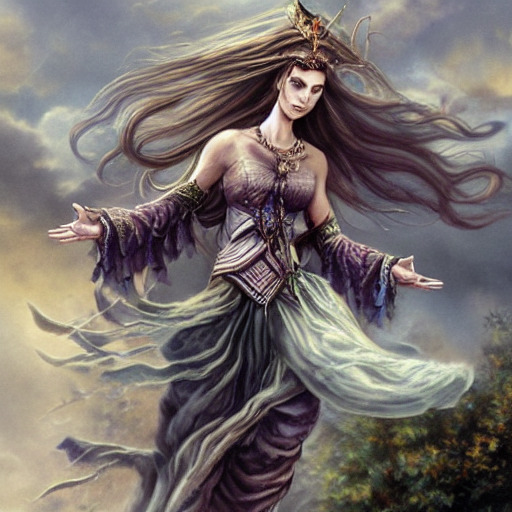
\includegraphics[width=\columnwidth]{feats/sphere focus aeromancy}
    \featpre Access to the \sphere{Aeromancy} \glossterm{mystic sphere}.

    \magicalff[1]{Distant Winds} You gain a \plus15 foot bonus to your range with ranged spells from the \sphere{Aeromancy} \glossterm{mystic sphere}.
    This does not affect spells that do not have a range listed in feet.

    \magicalff[6]{Windborne Spell} You learn an additional spell.
    The spell can be up to rank 3, even if you do not have access to rank 3 spells.
    When you cast that spell, choose a location within \shortrange of you.
    The spell takes effect as if you were in the chosen location.
    This affects your \glossterm{line of effect} for the ability, but not your \glossterm{line of sight} (since you still see from your normal location).
    Since an ability's range is measured from your location, this can allow you to affect targets outside your normal range.

    When you gain access to new spell ranks, you can change which spell you know with this ability, including spells with a higher rank.

    \magicalff[12]{Airborne} You gain a \glossterm{fly speed} equal to the \glossterm{base speed} for your size with a maximum height of 15 feet (see \pcref{Flight}).
    As a \glossterm{free action}, you can increase your \glossterm{fatigue level} by one to ignore this height limit until the end of the round.
    In addition, you gain a \plus15 foot bonus to the height limit of any fly speed you gain from \sphere{Aeromancy} spells.

    \magicalff[18]{Distant Winds+} The range bonus from your \textit{distant winds} ability increases to \plus60 feet.
  \end{magicalfeat}

  \begin{magicalfeat}{Sphere Focus: Aquamancy}{Casting, Magical}
    \featpre Access to the \sphere{Aquamancy} \glossterm{mystic sphere}.

    \magicalff[1]{Aquatic Propulsion} Once per round, after you make an attack with a spell from the \sphere{Aquamancy} \glossterm{mystic sphere}, you can \glossterm{push} yourself up to 10 feet.
    You can use this ability with \glossterm{strikes} using natural weapons from that sphere, such as from the \spell{aqueous tentacle} spell.
    The attack does not have to hit for you to use this ability.

    % TODO: it would be nice if this could be applied to spells you know from unusual sources, such as Elemental Spell.
    \magicalff[6]{Bubble Spell} You learn an additional spell.
    The spell can be up to rank 3, even if you do not have access to rank 3 spells.
    When you cast that spell, you can imbue it in a Small bubble of water that appears in your space.
    If you do, the spell does not take effect immediately, and you choose a location within \medrange of you.
    The bubble floats 15 feet through the air towards your chosen destination during each subsequent phase.
    It pops when it reaches its destination or hits an intervening obstacle.
    As normal for simultaneous actions, creatures cannot dodge the bubble by moving away in the same phase that it would reach them.

    When the bubble pops, the spell takes effect at the bubble's location as if you were there.
    A targeted spell only targets the creature or object that the bubble popped on.
    Area spells must have their point of origin where the bubble popped, but you can otherwise control their direction normally.
    This affects your \glossterm{line of effect} for the ability, but not your \glossterm{line of sight} (since you still see from your normal location).

    When you gain access to new spell ranks, you can change which spell you know with this ability, including spells with a higher rank.

    \magicalff[12]{Partially Liquid} You gain a \plus4 bonus to the Flexibility skill.
    In addition, you gain a \plus4 bonus to your defenses when determining whether a \glossterm{strike} gets a \glossterm{critical hit} against you instead of a normal hit.

    \magicalff[18]{Partially Liquid+} You are immune to \glossterm{critical hits} from \glossterm{strikes}.
  \end{magicalfeat}

  \begin{magicalfeat}{Sphere Focus: Astromancy}{Casting, Magical}
    \featpre Access to the \sphere{Astromancy} \glossterm{mystic sphere}.

    \magicalff[1]{Astral Spell Transit} You gain a \plus15 foot bonus to your range with abilities from the \sphere{Astromancy} \glossterm{mystic sphere}.

    \magicalff[6]{Transposing Spell} You learn an additional \glossterm{targeted} spell.
    The spell can be up to rank 3, even if you do not have access to rank 3 spells.
    When you cast the spell on a Large or smaller creature, you can switch places with the target.
    This requires an attack vs. Mental if the target is not an \glossterm{ally}.
    When you switch places, you \glossterm{teleport} into the target's location, and it teleports into your location.
    If the teleportation is invalid for either target, it fails for both targets.

    When you gain access to new spell ranks, you can change which spell you know with this ability, including spells with a higher rank.

    \magicalff[12]{Efficient Transit} You learn how to transport creatures and objects more smoothly between planes.
    The \glossterm{difficulty value} to hear noise caused by creatures and objects you \glossterm{teleport} increases by 10 (see \pcref{Teleportation Noise}).
    In addition, whenever you fail to teleport a creature or object due to specifying an invalid destination, you may immediately specify a different destination for that ability.
    If that second destination is also invalid, the ability fails normally.

    \magicalff[18]{Astral Spell Transit+} The range increase from your \textit{astral spell transit} ability increases to \plus30 feet.
    In addition, you gain a \plus15 foot bonus to your range with all \magical abilities that are not from the Astromancy mystic sphere.
  \end{magicalfeat}

  \begin{magicalfeat}{Sphere Focus: Channel Divinity}{Casting, Magical}
    \featpre Access to the \sphere{Channel Divinity} \glossterm{mystic sphere}.

    \magicalff[1]{Divine Retribution} Whenever a creature attacks you, you \glossterm{briefly} gain a \plus2 accuracy bonus against that creature.
    As normal, this bonus does not stack with itself.

    \magicalff[6]{Judging Spell} You learn an additional spell.
    The spell can be up to rank 3, even if you do not have access to rank 3 spells.
    When you cast the spell, each non-\glossterm{ally} affected by it \glossterm{briefly} takes a \minus1 bonus to all defenses.
    This penalty also affect any attacks made by the spell itself.
    If the spell did not affect any non-ally creatures, you \glossterm{briefly} gain a \plus1 bonus to all defenses.

    When you gain access to new spell ranks, you can change which spell you know with this ability, including spells with a higher rank.

    \magicalff[12]{Font of Divinity} Choose a spell you know with the \abilitytag{Attune} tag from the \sphere{channel divinity} mystic sphere.
    When you attune to that spell, you may also choose one \glossterm{ally} within \medrange.
    That ally can also choose to attune to the spell, and you both gain its benefits.
    When you stop attuning to that spell, your ally is also forced to stop attuning to the spell.

    Since you cannot attune to the same spell more than once, you cannot share the effects of the spell with more than one ally at a time in this way.
    You can change which spell you choose with this ability whenever you learn a new spell or gain access to a new spell rank.

    \magicalff[18]{Divine Retribution+} The bonus also applies against creatures that attack any of your \glossterm{allies}, not just you.
  \end{magicalfeat}

  \begin{magicalfeat}{Sphere Focus: Chronomancy}{Casting, Magical}
    \featpre Access to the \sphere{Chronomancy} \glossterm{mystic sphere}.

    \magicalff[1]{Accelerated Mind} You can perform mental tasks more quickly as normal.
    \glossterm{Mundane} mental actions that would normally take a \glossterm{standard action} instead take a \glossterm{minor action}.
    Long-term activities can be done twice as quickly as normal.
    This includes reading books, searching areas, and other similar activities.
    It does not affect spellcasting, performing rituals, or other similar magical abilities.

    \magicalff[6]{Quickened Chronomancy} You learn an additional spell from the \sphere{Chronomancy} mystic sphere.
    The spell can be up to rank 3, even if you do not have access to rank 3 spells.
    You can cast the spell as a \glossterm{minor action}.
    When you do, you \glossterm{briefly} become \slowed and cannot take standard actions.

    When you gain access to new spell ranks, you can change which spell you know with this ability, including spells with a higher rank.

    \magicalff[12]{Thief of Time} Whenever you cast a spell from the \sphere{Chronomancy} mystic sphere that deals damage to another creature or causes another creature to be \slowed, you \glossterm{briefly} gain a \plus20 foot bonus to your land speed.

    \magicalff[18]{Accelerated Mind+} Once per round, you can perform a purely mental action that would normally require a \glossterm{minor action} as a \glossterm{free action}.
    This can be used to sustain spells or perform other magical feats.
    However, you cannot use the same ability twice in the same round.
    In addition, the speed increase for long-term tasks from your \textit{accelerated mind} ability increases to five times normal speed.
  \end{magicalfeat}

  \begin{magicalfeat}{Sphere Focus: Cryomancy}{Casting, Magical}
    \featpre Access to the \sphere{Cryomancy} \glossterm{mystic sphere}.

    \magicalff[1]{Frozen Blood} You are \glossterm{impervious} to \atCold and \atPoison attacks.

    \magicalff[6]{Icy Carapace} You learn the \spell{icy shell} spell, or another spell from the \sphere{Cryomancy} mystic sphere if you already know that spell.
    In addition, the number of layers you can create with \spell{icy shell} increases by one.

    \magicalff[12]{Frozen Blood+} You are immune to \atCold and \atPoison attacks.

    \magicalff[18]{Icy Carapace+} The number of bonus layers you gain from your \textit{icy carapace} ability increases to two.
  \end{magicalfeat}

  \begin{magicalfeat}{Sphere Focus: Electromancy}{Casting, Magical}
    \featpre Access to the \sphere{Electromancy} \glossterm{mystic sphere}.

    \magicalff[1]{Electricity Tolerance} You are \trait{impervious} to \atElectricity attacks.

    \magicalff[1]{Extended Chain} The distance that your abilities can \glossterm{chain} is increased to 30 feet instead of 15 feet.

    \magicalff[6]{Chaining Spell} You learn an additional \glossterm{targeted} spell.
    The spell can be up to rank 3, even if you do not have access to rank 3 spells.
    It \glossterm{chains} one additional time, even if it did not originally chain.

    When you gain access to new spell ranks, you can change which spell you know with this ability, including spells with a higher rank.

    \magicalff[12]{Electricity Immunity} You are \trait{immune} to \atElectricity attacks.

    \magicalff[12]{Static Buildup} Whenever you use the \ability{sprint} ability, you gain a \plus2 accuracy bonus with your next spell from the \sphere{Electromancy} mystic sphere.
    This bonus disappears if not used before the end of the next round.

    \magicalff[18]{Extra Chain} All of your \glossterm{targeted} \sphere{Electromancy} spells \glossterm{chain} one additional time, even if they did not originally chain.
    If your \textit{chaining spell} ability affects a non-\sphere{Electromancy} spell, it also chains two additional times instead of only one.
  \end{magicalfeat}

  \begin{magicalfeat}{Sphere Focus: Enchantment}{Casting, Magical}
    \featpre Access to the \sphere{Enchantment} \glossterm{mystic sphere}.

    \magicalff[1]{Hidden Influence} You gain a \plus4 accuracy bonus with spells from the Enchantment mystic sphere against \unaware creatures.
    In addition, the \glossterm{difficulty value} to observe the effects of your \abilitytag{Emotion} abilities with the Awareness and Social Insight skills increases by 10 (see \pcref{Notice Subtle Effect}, and \pcref{Discern Enchantment}).

    \magicalff[6]{Mind Fragments} When you use a \magical ability that has the \abilitytag{Emotion} tag, you can affect creatures that are immune to that ability due to being \trait{mindless} or \trait{simple-minded}.
    You treat those creatures as being \impervious instead of immune.
    This does not allow you to affect creatures who are immune to those abilities for other reasons.

    \magicalff[12]{Sympathetic Enchantment} You learn an additional \glossterm{targeted} spell from the \sphere{Enchantment} mystic sphere.
    The spell can be up to rank 5, even if you do not have access to rank 5 spells.
    When you cast that spell, you can spend a \glossterm{minor action} to sympathetically link yourself to the spell's targets.
    If you do, you are target of that spell in addition to any other targets.
    In exchange, you roll all attacks for that spell twice, keeping the higher result.

    When you gain access to new spell ranks, you can change which spell you know with this ability, including spells with a higher rank.

    \magicalff[18]{Hidden Influence+} The accuracy bonus from your \textit{hidden influence} ability also applies against \partiallyunaware creatures.
    In addition, the \glossterm{difficulty value} increase from that ability increases to \plus20.

    \magicalff[18]{Mind Fragments+} You no longer treat those creatures as being impervious.
  \end{magicalfeat}

  \begin{magicalfeat}{Sphere Focus: Fabrication}{Casting, Magical}
    \featpre Access to the \sphere{Fabrication} \glossterm{mystic sphere}.

    \magicalff[1]{Fabricate Trinket+} The maximum size of the trinket you can create with your \textit{fabricate trinket} cantrip increases by one size category.
    You can also cast it with the \abilitytag{Sustain} (minor) tag.
    If you do, it lasts as long as you sustain it, and does not remove any previous trinkets you created with that cantrip.

    \magicalff[1]{Mighty Creator} You can use your \glossterm{power} in place of your Craft skill to create items with spells from the \sphere{Fabrication} mystic sphere.

    \magicalff[6]{Fabricated Armaments} You gain a \plus1 accuracy bonus with \glossterm{strikes} using weapons you created with spells from the Fabrication mystic sphere.
    In addition, you gain a \plus1 bonus to the Armor defense provided by body armor from the Fabrication mystic sphere.

    \magicalff[12]{Overbuilt Fabrication} You learn an additional spell from the \sphere{Fabrication} mystic sphere.
    The spell can be up to rank 5, even if you do not have access to rank 5 spells.
    When you cast the spell, you can spend a \glossterm{minor action} to expand its construction.
    If you do, the spell's area is doubled, and the hit points of any objects the spell creates are also doubled.

    When you gain access to new spell ranks, you can change which spell you know with this ability, including spells with a higher rank.

    \magicalff[18]{Fabricate Trinket+} The size increase from your \textit{fabricate trinket+} ability increases to two size categories.

    \magicalff[18]{Fabricated Armaments+} The accuracy bonus from your \textit{fabricated armaments} ability increases to \plus2.
  \end{magicalfeat}

  \begin{magicalfeat}{Sphere Focus: Photomancy}{Casting, Magical}
    \featpre Access to the \sphere{Photomancy} \glossterm{mystic sphere}.

    \magicalff[1]{Scour Vision} Whenever you cause a creature to become \dazzled with a spell from the \sphere{Photomancy} \glossterm{mystic sphere}, you \glossterm{briefly} become \trait{invisible} to that creature.
    This works even if the creature was already dazzled.
    The creature can still see everything other than you normally.

    \magicalff[6]{Hardlight Photomancy} You learn an additional spell from the \sphere{Photomancy} mystic sphere that does not have the \abilitytag{Sustain} or \abilitytag{Attune} tags.
    The spell can be up to rank 3, even if you do not have access to rank 3 spells.
    When you cast the spell, you can spend a \glossterm{minor action} to solidify the spell's light.

    If you do, the edges of any areas of \glossterm{brilliant illumination} created by the spell become physical barriers.
    These barriers provide \glossterm{cover} against attacks made across them, though they cannot be destroyed by damage.
    Moving through the barriers costs an additional ten feet of movement.
    The barriers are only at the edges of the brilliant illumination, so this does not affect movement or attacks entirely within or entirely outside of the illuminated area.

    When you gain access to new spell ranks, you can change which spell you know with this ability, including spells with a higher rank.

    \magicalff[12]{Solar Beacon} Whenever you make a creature lose \glossterm{hit points} with a spell from the \sphere{Photomancy} mystic sphere, that creature suffers consequences as if it had been struck by a beam of natural sunlight.
    This can be deadly for some creatures.

    \magicalff[12]{Unwavering Sight} You are immune to being \dazzled and \blinded.

    \magicalff[18]{Piercing Sight} You can see through solid objects and spell effects up to one inch thick.
    You can perceive the existence of obstacles thinner than that, but they do not inhibit your sight.
    This does not grant you \glossterm{line of effect} to anything you see in this way, since the obstacle still exists.
  \end{magicalfeat}

  \begin{magicalfeat}{Sphere Focus: Polymorph}{Casting, Magical}
    \featpre Access to the \sphere{Polymorph} \glossterm{mystic sphere}.

    \magicalff[1]{Augmented Body}
    \begin{magicalattuneability}{Augmented Body}{\abilitytag{Attune} (deep)}
      \abilityusagetime Can be triggered when you finish a \glossterm{short rest}.
      \rankline
      Choose a physical attribute: Strength, Dexterity, or Constitution.
      You gain a \plus1 \glossterm{enhancement bonus} to that attribute.
    \end{magicalattuneability}

    \magicalff[6]{Fleshbending Spell} You learn an additional spell.
    The spell can be up to rank 3, even if you do not have access to rank 3 spells.
    When you attack with the spell, if your attack beats a living creature's Fortitude defense, it takes a \minus4 penalty to its other defenses against that spell.

    When you gain access to new spell ranks, you can change which spell you know with this ability, including spells with a higher rank.

    \magicalff[12]{Augmented Body+} This loses the \abilitytag{Attune} (deep) tag and gains the \abilitytag{Attune} tag.

    \magicalff[12]{Malleable Flesh} You gain a \plus2 bonus to the Flexibility skill.
    In addition, you gain a \plus2 bonus to your defenses when determining whether a \glossterm{strike} gets a \glossterm{critical hit} against you instead of a normal hit.

    \magicalff[18]{Malleable Flesh+} The bonuses increase to \plus10.
  \end{magicalfeat}

  \begin{magicalfeat}{Sphere Focus: Prayer}{Casting, Magical}
    \featpre Access to the \sphere{Prayer} \glossterm{mystic sphere}.

    \magicalff[1]{Personal Blessing} You gain an additional \glossterm{attunement point}.
    You can only use that attunement point to attune to spells from the \sphere{Prayer} mystic sphere.

    \magicalff[6]{Sustained Blessing} Whenever you cast a spell from the \sphere{Prayer} mystic sphere with the \abilitytag{Attune} (target) tag that is not a \glossterm{deep attunement}, you can choose to replace that tag with the \abilitytag{Sustain} (minor) tag.
    When you do, you must cast the spell as a \glossterm{standard action}, even if it could normally be cast as a \glossterm{minor action}.
    You can only apply this ability to one spell at a time.

    \magicalff[12]{Sustained Blessing+} When you used your \textit{sustained blessing} ability, you can replace the tag with \abilitytag{Sustain} (free) instead of \abilitytag{Sustain} (minor).
    You can still only sustain one spell in this way at a time.

    \magicalff[18]{Shared Boon+} When you use your \textit{shared boon} ability, you can also target yourself or a third ally within range.
  \end{magicalfeat}

  \begin{magicalfeat}{Sphere Focus: Pyromancy}{Casting, Magical}
    \featpre Access to the \sphere{Pyromancy} \glossterm{mystic sphere}.

    \magicalff[1]{Spreading Flame} Whenever you cast a spell from the \sphere{Pyromancy} \glossterm{mystic sphere} with a standard area, you can increase its area to the next standard area category, to a maximum of a Gargantuan area.
    If you do, the spell deals no damage against targets that it misses, even if it would normally deal half damage.
    The standard area categories are: \smallarea, \medarea, \largearea, \hugearea, and \gargarea.

    \magicalff[1]{Fire Tolerance} You are \trait{impervious} to \atFire attacks.

    \magicalff[6]{Overheated Pyromancy} You learn an additional spell from the \sphere{Pyromancy} mystic sphere.
    The spell can be up to rank 3, even if you do not have access to rank 3 spells.
    When you cast the spell, you can spend a \glossterm{minor action} to \glossterm{briefly} overheat the spell.
    You roll all attacks for an overheated spell twice, keeping the higher result.
    After using this ability, you \glossterm{briefly} cannot use it again and are \vulnerable to \atCold attacks.

    When you gain access to new spell ranks, you can change which spell you know with this ability, including spells with a higher rank.

    \magicalff[12]{Friendly Fire} Whenever you deal damage to your \glossterm{allies} with a \atFire ability, you deal half damage.

    \magicalff[12]{Fire Immunity} You are \trait{immune} to \atFire attacks.

    \magicalff[18]{Spreading Flame+} When you use your \textit{spreading flame} ability, you can still get a glancing blow with the spell.
  \end{magicalfeat}

  \begin{magicalfeat}{Sphere Focus: Revelation}{Casting, Magical}
    \featpre Access to the \sphere{Revelation} \glossterm{mystic sphere}.

    \magicalff[1]{Oracle} Once per \glossterm{long rest}, you can gain the benefit of the \ritual{augury} ritual as a standard action.
    Using this ability does not increase your \glossterm{fatigue level}.

    \magicalff[6]{Prescient Spell} You learn an additional spell.
    The spell can be up to rank 3, even if you do not have access to rank 3 spells.
    As a \glossterm{minor action}, you can foresee the future of casting that spell.
    When you do, roll 1d10 and record the result.
    If you cast the spell, then the first time you attack with it this round, you must use this die result for the attack roll.
    This does not tell you whether your attack will hit, only high your roll will be.
    A 10 explodes as normal, but only when you actually cast the spell and make the attack, not when foreseeing the future.
    If you don't like the result, you can simply choose not to cast the spell this round, and the die result is ignored.
    Either way, you \glossterm{briefly} cannot use this ability again.

    When you gain access to new spell ranks, you can change which spell you know with this ability, including spells with a higher rank.

    \magicalff[12]{Blind Seer} You gain \trait{blindsense} with a 90 foot range (see \pcref{Blindsense}).
    If you already have blindsense, you increase its range by 90 feet.
    In addition, you gain \trait{blindsight} with a 30 foot range, allowing you to see without light (see \pcref{Blindsight}).
    If you already have blindsight, the range of your blindsight increases by 30 feet.

    \magicalff[18]{Oracle+} You can use your \textit{oracle} ability once per \glossterm{short rest} instead of once per long rest.
  \end{magicalfeat}

  \begin{magicalfeat}{Sphere Focus: Summoning}{Casting, Magical}
    \featpre Access to the \sphere{Summoning} \glossterm{mystic sphere}.

    \magicalff[1]{Empower Summon}
    \begin{magicalactiveability}{Empower Summon}[\abilitytag{Swift}]
      \abilityusagetime \glossterm{Minor action}.
      \rankline
      Choose one creature within \medrange that you created with a spell from the \sphere{Summoning} \glossterm{mystic sphere}.
      That creature gains a \plus2 bonus to its \glossterm{accuracy} and \glossterm{defenses} this round.
    \end{magicalactiveability}

    \magicalff[6]{Resummon}
    \begin{magicalactiveability}{Resummon}
      \abilityusagetime Standard action.
      \abilitycost One \glossterm{fatigue level}.
      \rankline
      Choose a spell from the \sphere{Summoning} mystic sphere that you are still \glossterm{attuned} to, even if all creatures created by that spell are dead.
      All effects of that spell, including any active creatures, immediately end.
      Then, you recreate all creatures from that spell as if you had just cast it.
      Those creatures do not act until the next round.
    \end{magicalactiveability}

    \magicalff[12]{Generosity} Whenever you \glossterm{attune} to an item or spell that is not a \glossterm{deep attunement}, you may use this ability.
    If you do, all creatures you create with the \sphere{Summoning} mystic sphere gain the benefit of all \glossterm{enhancement bonuses} from the chosen item or spell.
    It still affects you normally.
    You may only choose one attunement with this ability at a time.

    \magicalff[12]{Resummon+} You can use your \textit{resummon} ability as a \glossterm{minor action}.

    \magicalff[18]{Empower Summon+} The bonuses from your \textit{empower summon} ability increase to \plus4.
  \end{magicalfeat}

  \begin{magicalfeat}{Sphere Focus: Telekinesis}{Casting, Magical}
    \featpre Access to the \sphere{Telekinesis} \glossterm{mystic sphere}.

    \magicalff[1]{Efficient Hand} You can cast the \spell{distant hand} \glossterm{cantrip} as a \glossterm{minor action}, and you can \glossterm{sustain} it as a \glossterm{free action}.
    In addition, the distance you can move the object increases to 30 feet, as if you had that spell's rank 4 upgrade.

    \magicalff[6]{Violent Hand}
    \begin{magicalactiveability}{Violent Hand}
      \abilityusagetime Standard action.
      \rankline
      Choose a weapon you are proficient with and currently controlling using the \spell{distant hand} cantrip.
      Make a melee \glossterm{strike} using that weapon that deals \glossterm{extra damage} equal to half your \glossterm{power}.
      The strike comes from the weapon's location, not your location.
      Because this is a \magical ability, you use your \glossterm{magical power} to determine your damage instead of your \glossterm{mundane power} (see \pcref{Power}).

      % TODO: it would be nice if this scaled more strongly with the chosen weapon's stats?
      \rankline
      \rank{9} The extra damage increases to 1d6 \add half your power.
      \rank{12} The extra damage increases to 1d6 \add your power.
      \rank{15} The extra damage increases to 3d6 \add your power.
      \rank{18} The \glossterm{weapon damage} is doubled.
    \end{magicalactiveability}

    \magicalff[12]{Kinetic Spell} You learn an additional spell.
    The spell can be up to rank 5, even if you do not have access to rank 5 spells.
    Whenever you cast that spell, you can spend a \glossterm{minor action} to \glossterm{briefly} imbue it with kinetic force.
    When the spell deals damage to a Huge or smaller target, you \glossterm{knockback} that target 15 feet away from you.
    You can only knockback any individual creature or object once per round.
    After using this ability, you \glossterm{briefly} cannot use it again.

    When you gain access to new spell ranks, you can change which spell you know with this ability, including spells with a higher rank.

    \magicalff[18]{Multiple Hands} When you use the \spell{distant hand} cantrip, you can create two hands instead of one.
    This can allow you to hold multiple objects simultaneously, though you must still take separate actions to manipulate those objects in any way more complicated than simple movement.
    Alternately, you can hold a single object with two hands instead of one.
    This gives you a \plus1 bonus to your Willpower for the purpose of determining your \glossterm{weight limits}, and allows you to make two-handed attacks with \weapontag{Heavy} and \weapontag{Versatile Grip} weapons using your \ability{telekinetic strike} ability.
  \end{magicalfeat}

  \begin{magicalfeat}{Sphere Focus: Terramancy}{Casting, Magical}
    \featpre Access to the \sphere{Terramancy} \glossterm{mystic sphere}.

    \magicalff[1]{Earthen Alloys} You may treat iron, steel, and worked stone as if they were unworked stone for the purpose of spells from the \sphere{Terramancy} \glossterm{mystic sphere}.

    \magicalff[6]{Rocky Carapace} You learn the \spell{rocky shell} spell, or another spell from the \sphere{Terramancy} mystic sphere if you already know that spell.
    In addition, the number of layers you can create with that spell increases by one.

    \magicalff[12]{Earthen Alloys+} You may treat dirt, sand, glass, and all kinds of metal except for cold iron and adamantine as if they were unworked stone for the purpose of spells from the \sphere{Terramancy} \glossterm{mystic sphere}.

    \magicalff[18]{Rocky Carapace+} The number of bonus layers you gain from your \textit{rocky carapace} ability increases to two.
  \end{magicalfeat}

  \begin{magicalfeat}{Sphere Focus: Thaumaturgy}{Casting, Magical}
    \featpre Access to the \sphere{Thaumaturgy} \glossterm{mystic sphere}.

    \magicalff[1]{Mystic Power} You gain a \plus1 bonus to your \glossterm{magical power}.

    \magicalff[6]{Invented Spell} You learn an additional spell from any mystic sphere, even a mystic sphere you do not have access to.
    The spell can be up to rank 3, even if you do not have access to rank 3 spells.
    When you learn the spell, you can remove one of the following tags from that spell: \atAcid, \atAuditory, \atCold, \atCompulsion, \atEmotion, \atElectricity, \atFire, or \atVisual.
    You can also add one of those tags to the spell.
    In addition, you can replace one defense that the spell attacks with any one other defense not already referenced by the spell.

    When you gain access to new spell ranks, you can change which spell you know with this ability, including spells with a higher rank.

    \magicalff[12]{Countermagic}
    \begin{magicalactiveability}{Countermagic}[\abilitytag{Swift}]
      \abilityusagetime Standard action.
      \abilitycost See text.
      \rankline
      Choose a creature within \rngmed range of you.
      If the target uses a \magical ability as a standard action this round, that ability has no effect.
      When you negate an ability in this way, if that ability's rank was higher than your maximum rank, you increase your \glossterm{fatigue level} by one.
      After you use this ability, you \glossterm{briefly} cannot use it again, whether or not it actually negated a magical effect.

      If a creature is capable of using multiple abilities during a single phase, only the first ability it uses can be countered.
      This is common for \glossterm{elite} monsters.
    \end{magicalactiveability}

    \magicalff[18]{Mystic Power+} The bonus from your \textit{mystic power} ability increases to \plus2.
  \end{magicalfeat}

  \begin{magicalfeat}{Sphere Focus: Toxicology}{Casting, Magical}
    \featpre Access to the \sphere{Toxicology} \glossterm{mystic sphere}.

    \magicalff[1]{Poisonous Blood} Whenever you become poisoned by a contact or ingestion poison, such as by drinking poison or from an enemy's attack, your body naturally repurposes the poison.
    The poison has no effect on you, but your body gains a dose of natural poison.
    This has no effect on injury-based poisons, which affect you normally without being absorbed.

    Whenever a living creature makes you lose \glossterm{hit points} with a \glossterm{melee} strike using a non-Long weapon, you may have that creature become \glossterm{poisoned} by your choice of one of the poisons you store with this ability.
    This expends the dose of that poison.

    Poisons that you carry in your body with this ability automatically decay after 24 hours, regardless of the normal duration of the poison.
    You can store up to 3 doses in your body with this ability at a time.

    \magicalff[6]{Venomous Spell} You learn an additional spell.
    The spell can be up to rank 3, even if you do not have access to rank 3 spells.
    Whenever you damage a living creature with that spell, you can cause the creature to become poisoned with your choice of one of the poisons you store with your \textit{poisonous blood} ability.
    This expends the dose of that poison.
    You can poison multiple creatures simultaneously in this way, but it costs one poison dose per creature affected.

    When you gain access to new spell ranks, you can change which spell you know with this ability, including spells with a higher rank.

    \magicalff[12]{Poisonous Blood+} You can store up to 6 poison doses with your \textit{poisonous blood} ability.
    In addition, you become immune to all poisons that you do not absorb with that ability.

    \magicalff[18]{Bloodstream Corruption} Whenever you make a living creature lose hit points with a \sphere{Toxicology} spell or your \textit{venomous spell}, that creature becomes \vulnerable to all poisons as a \glossterm{condition}.
  \end{magicalfeat}

  \begin{magicalfeat}{Sphere Focus: Umbramancy}{Casting, Magical}
    \featpre Access to the \sphere{Umbramancy} \glossterm{mystic sphere}.

    \magicalff[1]{Lightbane} You can cast the \spell{suppress light} \glossterm{cantrip} from the Umbramancy mystic sphere as a \glossterm{minor action}, and you can \glossterm{sustain} it as a \glossterm{free action}.

    \magicalff[6]{Shadowspell} You learn an additional spell.
    The spell can be up to rank 3, even if you do not have access to rank 3 spells.
    You gain a \plus2 accuracy bonus with that spell against \glossterm{shadowed} targets.
    This stacks with any existing bonus the spell has against shadowed targets.

    When you gain access to new spell ranks, you can change which spell you know with this ability, including spells with a higher rank.

    \magicalff[12]{Shadow Jumper} While you are \glossterm{shadowed}, the distance you can teleport with spells from the \sphere{Umbramancy} mystic sphere is doubled.

    \magicalff[18]{Lightbane+} When you cast your \textit{suppress light} cantrip, you can choose to completely block all light in the area instead of dimming it to be \glossterm{shadowy illumination}.
    If you do, the maximum area is reduced to a \medarea radius, and you \glossterm{briefly} cannot cast it in this way again.
  \end{magicalfeat}

  \begin{magicalfeat}{Sphere Focus: Verdamancy}{Casting, Magical}
    \featpre Access to the \sphere{Verdamancy} \glossterm{mystic sphere}.

    \magicalff[1]{Verdant Allies} Your speed is not reduced when moving in heavy \glossterm{undergrowth}.
    In addition, you can are unaffected by \glossterm{cover} and \glossterm{concealment} from plants whenever doing so would be beneficial to you, as the plants move out of the way to help you.
    This prevents you from suffering a miss chance on your attacks, and also prevents creatures from using cover or concealment from plants to hide from you.

    \magicalff[6]{Residual Undergrowth} Whenever you cast a spell from the \textit{verdamancy} sphere, you may create either \glossterm{light undergrowth} or \glossterm{heavy undergrowth} in the area of the spell.
    The undergrowth persists \glossterm{briefly}.
    It appears on the ground within the area for area spells, or on the ground in all spaces occupied by each target of the spell for targeted spells.

    \magicalff[12]{Lifeweb Spell} You learn an additional spell.
    The spell can be up to rank 5, even if you do not have access to rank 5 spells.
    Whenever you cast that spell, you can choose another Small or larger plant or living creature within \medrange of you.
    The spell takes effect as if you were in that plant or creature's space.
    This affects your \glossterm{line of effect} for the ability, but not your \glossterm{line of sight} (since you still see from your normal location).

    When you gain access to new spell ranks, you can change which spell you know with this ability, including spells with a higher rank.

    \magicalff[18]{Verdant Army} Your \glossterm{allies} within a \largearea radius \glossterm{emanation} from you also gain the benefit of your \textit{verdant allies} ability.
  \end{magicalfeat}

  \begin{magicalfeat}{Sphere Focus: Vivimancy}{Casting, Magical}
    \featpre Access to the \sphere{Vivimancy} \glossterm{mystic sphere}.

    % Should this be more specific, like "animates"?
    \magicalff[1]{Hidden Life} You can treat nonliving creatures other than undead as if they were living creatures for the purpose of your abilities from the \sphere{Vivimancy} \glossterm{mystic sphere}.

    \magicalff[1]{Personal Vitality} You gain a bonus equal to your level to your \glossterm{hit points}.

    \magicalff[6]{Soulscar Spell} You learn an additional spell that does not have the \abilitytag{Attune} or \abilitytag{Sustain} tags.
    The spell can be up to rank 3, even if you do not have access to rank 3 spells.
    Any hit point loss that would be inflicted on a living creature by the spell is doubled.
    However, whenever you cast the spell, you lose hit points equal to its rank.

    When you gain access to new spell ranks, you can change which spell you know with this ability, including spells with a higher rank.

    \magicalff[12]{Life Suppression} You are no longer considered a living creature for the purpose of attacks against you.
    This means that attacks which only affect living creatures have no effect against you.

    \magicalff[18]{Personal Vitality+} The hit point bonus increases to twice your level.
  \end{magicalfeat}

  \begin{feat}{Stealth Specialization}{Skill}
    \featpre Stealth as a trained skill.

    \ff[1]{Specialization} You gain a \plus3 bonus to the Stealth skill.

    \ff[6]{Mobile Stealth} Your penalties for moving while hiding are reduced by 5.
    This allows you to move at half speed without penalty.

    \ff[12]{Specialization+} The bonus from your \textit{specialization} ability increases to \plus6.

    \ff[18]{Ambush the Unwary} You gain a \plus2 accuracy bonus against \unaware and \partiallyunaware creatures.
  \end{feat}

  \begin{feat}{Survival Specialization}{Skill}
    \featpre Survival as a trained skill.

    \ff[1]{Specialization} You gain a \plus3 bonus to the Survival skill.

    \ff[6]{Terrain Tolerance} You are unaffected by \glossterm{difficult terrain} and harmful natural terrain of any kind.
    If a skill check, such as Climb or Swim, would normally be required to move through the terrain, this ability does not help.

    \ff[12]{Specialization+} The bonus from your \textit{specialization} ability increases to \plus6.

    \ff[18]{Planar Survival} You are immune to damage and \glossterm{conditions} imposed by being on other planes.
    In addition, you gain a \plus5 bonus to checks and defenses related to planar effects, such as checks required to manipulate subjective gravity.
  \end{feat}

  \begin{feat}{Swiftrunner}{General}
    \featpre Dexterity 3.

    \ff[1]{Rapid Movement} You gain a \plus10 foot bonus to your \glossterm{land speed} during the \glossterm{action phase}.

    \ff[1]{Sprinter} When you use the \ability{sprint} ability, you can move up to triple your movement speed.

    \ff[6]{Rapid Movement+} The speed bonus applies all the time, rather than only during the action phase.

    \ff[6]{Water Runner} During your movement with the \textit{sprint} ability, you can move on water and similar liquids as if they were solid ground.

    \ff[12]{Long-Distance Runner} You gain a \plus2 bonus to your \glossterm{fatigue tolerance}.

    \magicalff[18]{Cloud Runner} During your movement with the \textit{sprint} ability, you can move on clouds, fog, and similar gaseous substances as if they were solid ground.

    \ff[18]{Rapid Movement++} The speed bonus increases to \plus20 feet.
  \end{feat}

  \begin{feat}{Swim Specialization}{Skill}
    \featpre Swim as a trained skill.

    \ff[1]{Specialization} You gain a \plus3 bonus to the Swim skill.

    \ff[6]{Swim Speed} You gain a \glossterm{swim speed} 10 feet slower than the \glossterm{base speed} for your size.
    If you already have a swim speed, you gain a \plus10 foot bonus to your swim speed.
    A successful Swim check to move allows you to move a distance equal to your swim speed.

    \ff[12]{Specialization+} The bonus from your \textit{specialization} ability increases to \plus6.

    \ff[18]{Earth Swimmer} You can swim through loose earth and dirt as if it were water.
    Your swim speed in earth is 10 feet, regardless of any bonuses or penalties that would normally apply to your swim speed.
    In addition, you take a \minus4 penalty to \glossterm{accuracy} and your Armor and Reflex defenses while swimming in this way.
    The earth and dirt around you blocks line of sight and line of effect, so you usually cannot used ranged attacks of any kind.
  \end{feat}

  \begin{magicalfeat}{Telepath}{General, Magical}
    \featpre Intelligence and Willpower sum to at least 3

    \magicalff[1]{Telepathy} You gain \glossterm{telepathy} with a 120 foot range (see \pcref{Telepathy}).
    If you already have telepathy, the range of your telepathy increases by 120 feet.

    \magicalff[6]{Telepathic Tribulation}
    \begin{magicalactiveability}{Telepathic Tribulation}[\abilitytag{Compulsion}]
      \abilityusagetime Standard action.
      \rankline
      Make an attack vs. Mental against one creature within half the maximum range of your \glossterm{telepathy}.
      You gain an accuracy bonus with this attack equal to half the sum of your Intelligence and Willpower.
      \hit \damagerankone.
      If the target loses \glossterm{hit points} from this damage, it becomes \stunned as a \glossterm{condition}.

      \rankline
      % increase to d2
      \featlevel{9} The damage bonus from your power increases to be equal to your power.
      % increase to d3ish
      \featlevel{12} The base damage increases to 1d10.
      % increase to d4ish
      \featlevel{15} The damage bonus increases to 1d6 per 3 power.
      % at r7, can upgrade condition
      \featlevel{18} The target becomes \confused instead of stunned.
    \end{magicalactiveability}

    \magicalff[12]{Read Mind}
    \begin{magicalsustainability}{Read Mind}{\abilitytag{Emotion}, \abilitytag{Subtle}, \abilitytag{Sustain} (standard)}
      \abilityusagetime Standard action.
      \rankline
      Make an attack vs. Mental against a creature within half the maximum range of your \glossterm{telepathy}.
      You use your full Intelligence or Willpower in place of half your Perception to determine your accuracy with this attack (see \pcref{Accuracy}).
      Whether you hit or miss, you cannot attack the target with this ability again until it finishes a \glossterm{short rest}.
      \hit You know the target's current thoughts and emotions.
      In addition to the obvious effects, this grants you a \plus5 bonus to Deception, Persuasion, Intimidate, and Social Insight attacks and checks against the target.
      This bonus does not stack with other effects that allow you access to the target's mind, such as \ability{read emotions}.
      You cannot directly search the target's mind for arbitrary thoughts or information.
      However, creatures often think about questions they are asked, and their thoughts may reveal much more than their words.
      \crit You can also delve through the target's mind to answer a specific question.
      You can pose a question to it mentally and search its mind to know the exact answer to that question.
      This takes five rounds of continuous concentration, and you can only get answers to one such question each time you use this ability.
      The process of searching a creature's mind in this way is no easier to notice than normal for a \abilitytag{Subtle} ability.

      \rankline
      You gain a \plus2 accuracy bonus for every 3 levels beyond 12.
    \end{magicalsustainability}

    \magicalff[12]{Telepathy+} You can maintain mental channels with up to 5 creatures at once with your telepathy.
    You can send separate thoughts to each creature.

    \magicalff[18]{Mindsight} You can perfectly see intelligent creatures within the maximum range of your telepathy.
    This functions like \trait{blindsight}, except that it only allows you to see creatures with an Intelligence of 0 or higher.

    \magicalff[18]{Telepathy++} The range of your telepathy increases by 120 feet.
  \end{magicalfeat}

  \begin{feat}{Toughness}{General}
    \featpre Constitution 2.

    \ff[1]{Fortified Body} You gain a \plus2 bonus to your Fortitude defense.
    In addition, you need half the normal amount of rest and sleep each day to function normally.
    For example, a human would only need four hours of sleep per night.
    This does not reduce the time required for you to take a \glossterm{long rest}.

    \ff[6]{Durable} You gain a bonus equal to your level to your \glossterm{hit points} and \glossterm{damage resistance}.

    \ff[12]{Fortified Body+} The defense bonus from your \textit{fortified body} ability increases to \plus4.
    In addition, you also only need half the normal amount of time to complete a \glossterm{long rest}.

    \ff[18]{Durable+} The bonuses increase to twice your level.
  \end{feat}

  \begin{feat}{Trickshot}{Combat}
    \featpre Dexterity 2, Intelligence 1.

    \ff[1]{Alchemical Arrow} As a standard action, you can apply a consumable alchemical item to an arrow.
    The item does not have its normal area or any other immediate effect.
    When you hit or \glossterm{glance} a target with a \glossterm{strike} using that arrow, the alchemical item has its normal effect on that target.
    The alchemical item makes its own attack roll separately from the attack roll for the strike.
    It only affects one target of the strike, even if the strike would normally affect multiple creatures or objects.
    If the alchemical item would normally affect an area, that area is centered on the target of the strike.
    Then, the alchemical item and the arrow are destroyed.

    At the end of the next round after you use this ability, the arrow and alchemical item are destroyed.

    \ff[6]{Combo Expertise} Whenever you use a consumable alchemical item, you \glossterm{briefly} gain a \plus1 accuracy bonus with strikes.
    Whenever you make a strike, you briefly gain a \plus1 accuracy bonus with consumable alchemical items.

    \ff[12]{Alchemical Arrow+} When you make a strike with the arrow, the alchemical item takes effect on the target even if the strike misses.
    You can also intentionally miss with the arrow while still delivering the alchemical item to its intended target, allowing you to apply healing potions and similar effects from a distance.
    Finally, the augmented arrow lasts one additional round before being destroyed.

    \ff[18]{Combo Expertise+} Both accuracy bonuses increase to \plus2.
  \end{feat}

  \begin{magicalfeat}{Twinhand Spellcaster}{Casting, Magical}
    \featpre Dexterity 2.

    \magicalff[1]{Twinhand Precision} You can always choose to use \glossterm{somatic components} to cast your spells (see \pcref{Ability Usage Components}).
    As long as you have two \glossterm{free hands}, you gain a \plus1 \glossterm{accuracy} bonus with spells that you cast using \glossterm{somatic components}.

    \magicalff[6]{Freehand Implement} You can gain the benefits of up to two magical implements, such as staves or wands, without having to hold them in your hands.
    You must still have them on your person, such as in a pocket or strapped to your back, and you must still be attuned to them to gain their benefits.
    In addition, if your legacy item is an apparel item, you may choose both apparel and implement magic item effects for it.

    \magicalff[12]{Twinspell}
    \begin{magicalactiveability}{Twinspell}
      \abilityusagetime Standard action.
      \abilitycost Two \glossterm{fatigue levels}.
      \rankline
      You can only use this ability if you have two \glossterm{free hands}.

      Choose two spells that you know.
      You cast both spells simultaneously, one with each hand.
      This gives the spells \glossterm{somatic components}, regardless of any other effects which would would normally prevent you from requiring somatic components.
      Both spells must affect completely different targets, with no overlap between their targets or areas (if any).
      You cannot use the \ability{desperate exertion} ability to affect either spell.
    \end{magicalactiveability}

    \magicalff[18]{Twinhand Precision+} The bonus from your \textit{twinhand precision} ability increases to \plus2.
  \end{magicalfeat}

  \begin{feat}{Twin-Weapon Fighting}{Combat}
    \featpre Dexterity 2.

    \ff[1]{Twin-Wielding} You are considered to be twin-wielding while two of your hands are each wielding an identical weapon that you are proficient with.
    Each hand must hold a different weapon, rather than simply holding a heavy weapon in two hands.
    You can use \glossterm{natural weapons} to meet this condition, such as claws, as long as your hand is exclusively dedicated to using the natural weapon and not holding or being used for anything else.
    Several abilities from this feat only function while you are twin-wielding.

    \ff[1]{Paired Precision} You gain a \plus1 bonus to \glossterm{accuracy} with \glossterm{strikes} using weapons that you are twin-wielding.

    \magicalff[6]{Paired Legacy} If you would choose a weapon as your \glossterm{legacy item}, you can instead choose two identical weapons.
    Both weapons share the same properties from your legacy item.

    \ff[6]{Twin-Weapon Stance} At the start of each round, you can enter one of the stances below or change which stance you are in.
    You can maintain that stance as long as you are twin-wielding.
    % TODO: do fancy balance math
    \begin{itemize}
      % Alternate idea: allow glancing blows?
      \item Balanced: You gain a \plus1 bonus to your Armor defense.
        This bonus is considered to come from a shield, and it does not stack with the benefits of using any other shield.
      \item Deflecting Offhand: You gain a \plus3 bonus to your Armor defense.
        However, you cannot make \glossterm{dual strikes}.
        This bonus is considered to come from a shield, and it does not stack with the benefits of using any other shield.
        % If glancing with dual strikes becomes possible, that should count here
      \item Offhand Precision: When you make a dual strike, if you miss with one weapon, you gain a \plus4 accuracy bonus against the same target with the second weapon.
      \item Steady Hands: You gain a \plus2 accuracy bonus with dual strikes.
        However, you cannot get \glossterm{critical hits} with dual strikes.
    \end{itemize}

    \ff[12]{Potent Pairing} You gain a \plus1 bonus to your \glossterm{weapon damage} with weapons that you are twin-wielding.

    \ff[18]{Paired Precision+} The accuracy bonus increases to \plus2.
  \end{feat}

  \begin{magicalfeat}{Wardweaver}{Casting, Magical}
    \featpre Knowledge of a spell with the \abilitytag{Barrier} tag.

    \magicalff[1]{Hardened Barriers} Objects you create using abilities with the \abilitytag{Barrier} \glossterm{ability tag} gain a bonus equal to your \glossterm{power} to their \glossterm{damage resistance}.
    In addition, they treat all damage as being \glossterm{environmental damage}, so their damage resistance is never reduced (see \pcref{Environmental Damage}).

    \magicalff[6]{Defensive Barriers} You gain a \plus1 bonus to your Armor defense.
    In addition, objects you create with \abilitytag{Barrier} abilities have minimum defenses equal to 5 \add half your level.
    If the object already has specific defenses listed, it gains a \plus2 bonus to those defenses.

    \magicalff[12]{Barrier Spell} You learn a spell with the \abilitytag{Barrier} ability tag from any \glossterm{mystic sphere} that your \glossterm{magic source} gives access to, even if you do not have access to that mystic sphere.
    When you gain access to new spell ranks, you can change which Barrier spell you know.

    \magicalff[18]{Defensive Barriers+} Your Armor defense bonus from your \textit{defensive barriers} ability increases to \plus2.
    In addition, objects you create with \abilitytag{Barrier} abilities gain an additional \plus2 bonus to their defenses.

    \magicalff[18]{Hardened Barriers+} The damage resistance bonus from your \textit{hardened barriers} ability increases to twice your \glossterm{power}.
  \end{magicalfeat}

  \begin{feat}{Weapon Focus}{Combat}
    \ff[1]{Focused Weapon} Choose one type of weapon, such as a broadsword.
    This is your focused weapon, and your abilities from this feat give you benefits with your focused weapon.

    \ff[1]{Precise Focus} You gain a \plus1 accuracy bonus with your focused weapon.

    \ff[6]{Enhanced Legacy} If you choose your focused weapon as your \glossterm{legacy item}, you can choose an additional magic item property with a maximum rank of 3.

    \ff[12]{Enhanced Legacy+} You can change the item property, and the maximum rank increases to 5.

    \ff[12]{Precise Focus+} The accuracy bonus increases to \plus2.

    \ff[18]{Enhanced Legacy++} You can change the item property, and the maximum rank increases to 7.

    \ff[18]{Personalized Weapon} Choose one of the following \glossterm{weapon tags}: Clinch, Impact, Keen, Maneuverable, Parrying, Resonating, or Thrown (30/60).
    You treat your focused weapon as if it had that tag (see \pcref{Weapon Tags}).
  \end{feat}

  \begin{feat}{Whirlwind Warrior}{Combat}
    \featpre Dexterity 2.

    \ff[1]{Unfettered Movement} You can move through spaces occupied by enemies as if they were unoccupied.

    \ff[6]{Cyclone}
    \begin{sustainability}{Cyclone}{\abilitytag{Sustain} (standard)}
      \abilityusagetime Standard action.
      \rankline
      When you use this ability, make a melee \glossterm{strike} with 1d4 \glossterm{extra damage}.
      The strike targets all \glossterm{enemies} adjacent to you.
      During each of your subsequent actions, you can move up to half your \glossterm{land speed} and make a melee \glossterm{strike}.
      The strike targets all \glossterm{enemies} adjacent to you at any point during your movement.

      \rankline
      \featlevel{9} The extra damage increases to be equal to half your power.
      \featlevel{12} The extra damage increases to be equal to your power.
      \featlevel{15} The extra damage increases to 1d8 \add your power.
      \featlevel{18} The strike deals double \glossterm{weapon damage}.
    \end{sustainability}

    \ff[12]{Eye of the Storm} You take no penalties for \squeezing with other creatures.
    This does not reduce your penalties for squeezing in tight spaces.

    \ff[18]{Storm's Heart} You gain a \plus2 bonus to your Armor and Reflex defenses against creatures that you are sharing space with.
  \end{feat}

\section{Other Feat Rules}

  \subsection{Retraining Feats}
    At every level, you can choose to retrain an old feat in exchange for a new feat.


\chapter{Optional Rules}

This chapter describes a variety of optional rules that the GM can choose to use in their campaign.
These rule changes change the tone of the game, making it more gritty or more tactical.
They can also provide more detailed character customization options, increasing character uniqueness but potentially increasing the complexity of character creation.

\section{Attributes}

  \subsection{Other Methods of Attribute Generation}
    Point buy offers the fairest and most customizable system for determining attribute scores, ensuring that players can be almost any character they want to be. However, some groups may wish to determine attribute scores differently. Other options are provided below.

    \subsubsection{Simple Random Point Buy}
      With this method, you have only a small degree of control over your attribute scores, but all characters generated in this way are equally powerful.
      As with the point buy method, all your attribute scores start at 0, and you get 15 points to distribute among your attribute scores.
      However, you do not have full control over how to distribute those points.

      For each attribute, starting with the attributes you care about most, roll 1d8.
      You spend that many points on that attribute, ignoring any extra points that can't be spent
      For example, if you roll a 4, you spend 3 points on the attribute, causing you to start with a 2.
      If you do not have enough points remaining to spend the amount indicated by the die roll, spend as many as you can and move on to the next attribute.

      If you have points remaining after rolling all of your attribute scores, you may distribute the points freely among your abilities, using the normal point buy rules.
      You cannot increase the starting value of any individual attribute by more than 1 during this stage.
      If any of your attributes start as a 0, you may choose to lower them to gain the normal benefits from having low attributes (see \pcref{Attribute Penalties}).

      To further limit your character creation options, you may choose to randomize the order in which you roll your attributes instead of rolling them in an order of your choice.

    \subsubsection{Smoothed Random Point Buy}
      This method functions like the Simple Random Point Buy method, except that the resulting attribute values have a smoother distribution, and you can randomly end up with attribute penalties.

      For each attribute, starting with the attributes you care about most, roll 4d6.
      Then, remove any one of the rolls after seeing the results.
      Sum the results of the remaining three dice and spend the appropriate number of attribute points as indicated in \trefnp{Smoothed Random Point Buy Results}.
      If you do not have enough points remaining to spend the amount indicated by the die roll, spend as many as you can and move on to the next ability.

      If you have points remaining after rolling all of your attribute scores, you may distribute the points freely among your abilities, using the normal point buy rules.
      You cannot increase the starting value of any individual attribute by more than 1 during this stage.

      To further limit your character creation options, you may choose to randomize the order in which you roll your attributes instead of rolling them in an order of your choice.

      \begin{dtable}
        \lcaption{Smoothed Random Point Buy Results}
        \begin{dtabularx}{\columnwidth}{X X X}
          \tb{Roll} & \tb{Attribute} & \tb{Point Cost} \tableheaderrule
          3-4       & \minus2        & 0\fn{1} \\
          5-6       & \minus1        & 0\fn{2} \\
          7-8       & 0              & 0       \\
          9-10      & 1              & 1       \\
          11-12     & 2              & 2       \\
          13-15     & 3              & 3       \\
          16-18     & 4              & 5       \\
        \end{dtabularx}
        1 You gain one \glossterm{insight point}. \\
        2 You gain an additional \glossterm{trained skill}. \\
      \end{dtable}

    \subsubsection{Classic Hardcore}

      This method is completely random and can generate very overpowered or underpowered characters.
      It represents the unfairness of the world, where some people are just better or worse than others.
      For each attribute, roll 2d6, take the average (rounded down), and subtract 2.
      If you roll a 1 on both dice, treat the average as a 0.
      The result is your base value for that attribute.

\section{Epic Fates}
  After 21st level, characters no longer gain levels normally.
  However, they can still increase their personal power as they make progress towards their ultimate fate.

  When you reach 21st level, you may choose an epic fate that you qualify for, or you may delay choosing until you meet the prerequisites for your desired fate.
  You do not start with any ranks in you chosen epic fate.
  Each epic fate specifies ways that you can make progress towards that epic fate.
  Whenever you make dramatic progress towards your epic fate, your rank in that epic fate may increase, at the discretion of the Game Master.

  None of the epic fate abilities have a tag to indicate that they are \magical abilities.
  Many of them are not fundamentally \glossterm{mundane} in nature, but they are beyond normal magic, and effects like an \spell{antimagic field} cannot interact with or suppress them.

  \subsection{Artificial Immortality}
    You have sought out strange magical power in search of a way to artificially prolong your life.
    As your power grows, you become increasingly able to resist death and return from it.
    Eventually, you will transcend death entirely.

    \parhead{Prerequisites} You must perform a series of rituals to prepare yourself for immortality, at least one of which must be rank 7 or higher. There are many kinds of immortality that you can pursue with this epic fate, and the exact nature of the rituals will change depending on the type of immortality you pursue.

    \parhead{Progression} You must discover powerful new magic rituals that support your particular form of immortality. This generally requires exploring sites of ancient magic, gaining favor with powerful creatures who have relevant knowledge or abilities, and independent experimentation based on your findings.

    \subsubsection{Artifical Immortality Ranks}

      \parhead{Rank 1 -- Life After Death} If you die from any cause other than old age, you resurrect according to nature of your chosen path to immortality.
      For example, you can have a phylactery regenerate a new body for you like a lich, or you can create clones of yourself or golems that you inhabit if your first body dies.
      You must always return in a new body of some sort.

      Your specific form of immortality determines where you return, such as at the site of your death or at your personal sanctum.
      However, it cannot cannot be based on the location or state of your old corpse, since that corpse is no longer ``you''.
      The timing of your resurrection may also differ based on your immortality, but you cannot complete your resurrection sooner than one day after the time of your death. After you resurrect in this way, this ability does not function for one week, allowing you to be killed normally.

      This immortality may change your base species, such as if you become a lich or move your body into a flesh golem. If it does, you retain all benefits and modifiers from your original species other than size, and you gain the effects of the new species in addition.

      \parhead{Rank 2 -- Death Familiarity} You become so familiar with the trauma of injury and death that your mind and body adapt to it.
      You gain a \plus10 bonus to vital rolls.
      In addition, the time of your vulnerability to true death after resurrection is reduced to 48 hours.

      \parhead{Rank 3 -- Artificial Life} Whenever you resurrect with your \textit{life after death} ability, your new body gains a \plus2 bonus to two random attributes. The attributes are randomized differently for each new body. In addition, that resurrection functions even if the cause of your death was old age, and you can control the physical age of your new body.

      \parhead{Rank 4 -- Deathcaller} You are deeply familiar with death, and know how to most effectively inflict it on others.
      Whenever you cause a living creature to lose at least half its hit points in a single round, you may kill that creature outright.
      In addition, your \textit{artificial life} ability grants a bonus to three random attributes instead of two random attributes.

      \parhead{Rank 5 -- True Immortality} You become fully immortal. There is no time limit after the resurrection from your \textit{life after death} ability where you become vulnerable to a true death. In addition, the resurrection can complete as quickly as one minute after your death. If a physical component limits your immortality, such as a phylactery, it can no longer be damaged or destroyed without the direct intervention of a rank 5 Slayer.

  \subsection{Ascendant}
    You have begun to see through the weave of the world and glimpse the higher truths beyond.
    As your insight into the true nature of reality grows, you begin to transcend the physical realm.
    Eventually, you become a being of pure energy.

    \parhead{Prerequisites} You must have spent at least a week living in each of the following planes: Air, Astral, Earth, Fire, Material, and Water.
    In addition, you must have an Intelligence or Perception of at least 2.

    \parhead{Progression} You must discover and spend time in exotic environments with unusual properties, especially with energy-related phenomena, to discern the underlying structure of the universe revealed in extremes.
    This involves a mix of meditation, observation, and potentially dangerous personal experience.
    Discovering potentially valuable locations may require extensive research.
    In order to reach the highest ranks, you must journey into forbidden realms of powerful magic, like the inner sanctums of major deities or the horrific depths of the Eternal Void.

    \subsubsection{Ascendant Ranks}

      \parhead{Rank 1 -- Energetic Soul} Whenever you deal damage, you can treat at as energy damage in addition to its other types.
      In addition, whenever you take or deal energy damage while not \trait{incorporeal}, you and your equipment \glossterm{briefly} become incorporeal.
      While you are incorporeal in this way, all of your other movement modes are replaced with a \glossterm{fly speed} equal to your base speed (see \pcref{Flight}).
      This flight has a \glossterm{height limit} of 60 feet.
      Since you have no land speed, flying in this way does not penalize your Armor or Reflex defenses.

      \parhead{Rank 2 -- See Through the Weave} You can see everything within 120 feet of you perfectly, regardless of obstacles of any kind or light levels.
      This is similar to \trait{blindsight}, except that it also ignores solid obstacles of any kind, allowing you to have \glossterm{line of sight} through walls.
      You can perceive the presence of obstacles just as well as you can see what lies behind them.

      \parhead{Rank 3 -- Reach Through the Weave} When you use any of your abilities, you can treat yourself as being up to 60 feet away from your true location.
      You do not need \glossterm{line of effect} to your chosen location.
      For example, this allows you to make melee attacks against creatures up to 60 feet away.
      This changes your \glossterm{line of effect}, but does not change your \glossterm{line of sight}.

      % Does this need to have an explicit Recover reminder? Seems like that just works as intended
      \parhead{Rank 4 -- Become Energy} You become permanently \trait{incorporeal}, along with any equipment you carry.
      The fly speed from your \textit{energetic soul} ability also becomes permanent.
      In addition, you no longer age and no longer have hit points.
      Instead, you gain a bonus to your \glossterm{damage resistance} equal to the number of hit points you would normally have from your level, base class, and Constitution.
      Other effects that would increase or decrease your maximum hit points have no effect on you.
      You gain vital wounds based on taking damage in excess of your damage resistance rather than in excess of your hit points, including the extra vital wounds for taking massive damage.

      \parhead{Rank 5 -- Ascension} You cannot be killed, only dissipated.
      When you die, you automatically reform at a random location within a mile of your death after 10 minutes.
      Reforming in this way returns you to full damage resistance and removes all conditions and vital wounds, but your \glossterm{fatigue levels} and other effects remain the same.

  \subsection{Deity}
    People have begun to worship you, putting you on the path to become a deity.
    As your followers grow, you become capable of ever greater miraculous acts, and you can grant your followers some of your power.
    Eventually, you ascend into the pantheon of gods.

    \parhead{Prerequisites} You must have at least a hundred worshippers with souls to choose this epic fate.
    In addition, you must not have any cleric archetypes.

    \parhead{Progression} To progress towards this epic fate, you must gain a significant number of additional worshippers.
    In general, you must at least double your worshippers to progress towards each new rank of this fate, though this can vary widely.
    Having worshippers among many different places is more valuable than converting an isolated group to worship you, though both are helpful.

    \subsubsection{Deity Ranks}
      \parhead{Rank 1 -- Domain Influence} Choose a cleric domain.
      You gain all abilities from that domain except for its mastery ability.
      In addition, your worshippers become eligible to gain cleric archetypes, though they cannot exceed a maximum rank in those archetypes of twice your rank in this epic fate (to a maximum of 8).
      This does not grant additional archetypes to worshippers who have already chosen their three archetypes, and is usually only relevant to NPC worshippers.

      \parhead{Rank 2 -- Prayers} You hear all prayers directed to you.
      Once per week, you can teleport yourself and up to ten \glossterm{allies} any distance within the same plane as a \glossterm{standard action}.
      Your destination must either be a worshipper actively praying to you or a holy place dedicated to you.
      In addition, choose a second cleric domain.
      You gain all abilities from that domain except for its mastery ability.

      \parhead{Rank 3 -- Domain Mastery} Choose a third cleric domain.
      You gain all abilities from that domain.
      In addition, you gain the mastery ability from the domains you chose with your \textit{domain influence} and \textit{prayers} abilities.

      \parhead{Rank 4 -- Demigod} You become a demigod.
      You no longer age normally, and you cannot die from old age.
      You become a planeforged native to an Aligned Plane matching your alignment.
      For details about the aligned planes, see the Tome of Guidance.
      While you are on that plane, you can teleport to any plane with your \textit{prayers} ability from this epic fate.
      In addition, you can use that teleportation ability once per hour instead of once per week.

      \parhead{Rank 5 -- Deification} You become a deity.
      You are transported to an Aligned Plane matching your alignment, and you gain divine dominion over an amount of territory in that plane.
      While you are in your territory, you can can freely reshape your territory with a thought to match your desires, and you are immune to all damage and \glossterm{conditions}.

      Regardless of which plane you are on, you can teleport to anywhere within your home plane as a \glossterm{standard action}.
      In addition, there is no limit on the number of times you can teleport with your \textit{prayers} ability from this epic fate.

  \subsection{Hero of Legend}
    You are widely known as a hero, rescuing those in need.
    As your deeds of heroism spread, you gain abilities to help you protect others.
    Although you will eventually die, your legend will live on, inspiring others to save people as you did.

    \parhead{Prerequisites} You must be publicly known to be involved with saving at least one major country or similarly large group of people from some sort of disaster to choose this epic fate.

    \parhead{Progression} To progress towards this epic fate, you must publicly contribute to saving large numbers of people from death or other major disasters in a way that builds your reputation.
    Reaching the higher ranks typically requires saving a significant fraction of a major plane from some sort of catastrophe.

    \subsubsection{Hero of Legend Ranks}
      \parhead{Rank 1 -- Worthy Hero} You and all \glossterm{allies} who can see or hear you are immune to being frightened and panicked.
      In addition, you gain a \plus100 bonus to your \glossterm{hit points}.

      \parhead{Rank 2 -- Heroic Intervention} As a \glossterm{free action}, you may choose any number of \glossterm{allies} within \shortrange of you.
      Whenever a chosen creature would be attacked that round, that attack is made against you instead.
      If the attack would have targeted both you and that ally, the attack only targets you once, not twice.
      This ability has the \abilitytag{Swift} tag.

      \parhead{Rank 3 -- Invincible Hero} You gain a \plus4 bonus to all defenses.
      In addition, you cannot be \vulnerable for any reason.

      \parhead{Rank 4 -- Answer the Call} You gain an intuitive sense for when people need your aid.
      Whenever someone on the same plane as you is in danger, you are aware of the existence of that danger.
      You can sense the general category of danger (fire, combat, drowning, etc.) and a very approximate direction and distance.
      This generally allows you to sense if a large number of people are in danger from the same thing.
      As a \glossterm{standard action}, you can teleport any distance within that plane to reach a person in danger.

      \parhead{Rank 5 -- Heroic Legacy} If you die, your legend lives on.
      You may choose a worthy successor, either before your death or after your death from your afterlife plane.
      When you die, or as soon as you choose a successor while dead, your successor immediately gains the Rank 1 benefit from this archetype.
      As long as your successor lives and remains worthy, you cannot choose to be resurrected from your afterlife.
      As a player, you may choose to play as your successor instead of your original character if the GM allows it.

  \subsection{Mutant}
    Your body has been altered by battle scars and strange experiments.
    As your mutations grow ever more extreme, you become more powerful - and more monstrous.
    Eventually, you can regenerate from death itself, though some scars never fade.

    \parhead{Prerequisites} Dangerous experiments to mutate your body in extreme ways must have been performed on you.
    You can choose the nature of these experiments, such as alchemical or magical.
    Some mutants do this to themselves, while others find willing collaborators.
    In addition, you must have a Constitution of at least 2.

    \parhead{Progression} To progress towards this epic fate, you must continue ever more radical forms of experimentation.
    As you become inured to ordinary alterations to your body, you must travel and research to find unique substances of immense power to fuel the experiments.
    To reach the higher ranks, you must undergo experiments that kill you far more often than they succeed, so you will need to be resurrected multiple times to continue down this path.

    \subsubsection{Mutant Ranks}
      \parhead{Rank 1 -- Unnatural Arsenal} You grow an extra functioning arm and hand.
      In addition, you gain a wide variety of natural weapons (see \tref{Natural Weapons}).
      You gain a bite, horn, ram, stinger, and tentacle.
      In addition, two of your hands become claws.
      You gain these weapons in addition to any natural weapons you already have, no matter how biologically implausible that may be.
      % TODO: mutants will often have Massive, so Sweeping is oddly redundant.
      In addition, each of your natural weapons has the \weapontag{Sweeping} (3) weapon tag in addition to its other weapon tags.

      \parhead{Rank 2 -- Regeneration} At the end of each round, you regain hit points equal to a quarter of your maximum hit points.
      In addition, you may increase the result of one of your \glossterm{vital wounds} by 1, to a maximum of 10.
      If you are unconscious, this automatically applies to your most severe vital wounds first.

      \parhead{Rank 3 -- Monstrous Form} Your size increases by one size category.
      In addition, you gain a wide variety of movement modes.

      You gain a \glossterm{climb speed} and \glossterm{swim speed} equal to your base speed, and a 10 foot \glossterm{burrow speed}.
      For each of those movement modes, if you already have it, you gain a \plus10 foot bonus to your speed with that movement mode instead.
      Wings also grow from your back, granting you a \glossterm{fly speed} equal to your base speed with a 60 foot \glossterm{height limit} (see \pcref{Flight}).

      \parhead{Rank 4 -- Two Heads Are Better Than One} You grow a second head.
      Whenever you gain a \glossterm{condition}, you choose which head gains the condition, with the restriction that the chosen head must not already have more conditions than the other head.
      At the start of each round, you can choose which heads are active during that round.
      You are only subject to the effects of the conditions affecting active heads.
      If you choose for both heads to be active, you can use an extra \glossterm{minor action} during the \glossterm{action phase}.

      \parhead{Rank 5 -- Regenerative Immortality} You can regenerate from any wounds, even lethal ones.
      When you die, your \textit{unnatural regeneration} ability continues functioning.
      Once that ability improves your vital wounds so they are all above 0, you return to life.
      However, each time you die, you gain a new scar that your regeneration always recreates.

      If your corpse is mutilated, burned, immersed in acid, or fully destroyed, this process can take much longer to complete, but it cannot be fully stopped.
      Some drop of blood, flake of skin, or other remnant of your corpse will always persist and regenerate eventually.
      If your body is separated into pieces while you are dead, each piece will attempt to regenerate individually.
      Your soul will automatically return to the first piece that regenerates completely, at which point the remaining fragments will wither and die.

  \subsection{Paradox}
    You exist partly outside of the ordinary flow of time.
    Your very existence wreaks havoc on prophecies and the orderly sequence of events.
    As your alterations to the natural timeline of the universe grow in scope, your ability to bend time to your whims grows in turn.
    Eventually, you become a fixed point across all of time.

    \parhead{Prerequisites} You must have been directly involved with an action that resulted in a significant change to at least one major country or similarly significant entity.
    Any type of change is acceptable, as long as it would be historically important would not have happened without your intervention.

    \parhead{Progression} To progress towards this epic fate, you must be alter the course of other major events that will be remembered to history.
    Reaching the higher ranks typically requires changing the fate of major planes, or creatures of similar importance.

    \subsubsection{Paradox Ranks}
      \parhead{Rank 1 -- Temporal Aberration} Your actions, and events involving you, cannot be observed in any effect that sees or predicts the future.
      This applies against both magical abilities and abilities that rely on direct observation.
      Prophecies are only able to describe how events would happen without your intervention, and are blind to any changes you might cause.

      In addition, whenever you would make a \glossterm{movement}, you can make two different movements and then decide which one was the movement you actually made.
      You can make this decision after observing how other creatures react to your movement, but before taking any other actions.

      The other movement never happened, and had no effect.
      Only the movement itself is reverted in this way.
      Any other abilities you used during the resolution of that movement, such as the \ability{sprint} ability, still happened, so you would still gain fatigue and resolve other effects.

      \parhead{Rank 2 -- A Fork In Time's Road} Whenever you would take a standard action, you can take two different standard actions and then decide which one was the action you actually took.
      You can make this decision after seeing all die results and observing all effects of both actions, but before taking any other actions.

      The other action never happened, and has no effect.
      Only the standard action itself is reverted in this way.
      Any other abilities you used during the resolution of that action, such as the \ability{desperate exertion} ability, still happened, so you would still gain fatigue and resolve other effects.

      \parhead{Rank 3 -- Choose Fate} Once per \glossterm{short rest}, whenever you or any other creature you are aware of rolls an attack or check, you can choose the result of that die.
      You can choose to use this ability after learning the result of the action using that die roll, including whether it succeeded or failed and the result of any damage dice based on the attack.
      However, you must use it before any other actions resolve.
      If you use this to make an attack \glossterm{explode}, subsequent dice after the die you modify in this way are rolled normally.
      Using this to affect an enemy's action may change the actions taken by other enemies in that enemy's \glossterm{allied group}, which the GM should resolve.

      \parhead{Rank 4 -- Paradoxical Defense} Whenever a creature attacks you, it must roll twice and take the lower result.
      This does not protect any other targets of the attack.

      \parhead{Rank 5 -- Fixed Point} You become an immutable fact across all of time.
      You no longer age.
      Whenever you die, history is rewritten so you retroactively never died instead.
      The changes are as subtle and believable as possible, but even extraordinary coincidences can occur to save you from death.
      You typically still end up unconscious from vital wounds, and are always removed from combat or otherwise unable to usefully act for at least ten minutes, but you survive.

  \subsection{Slayer}
    You are a killer of legendary skill.
    As your body count increases, you gain abilities to help you track down and kill increasingly powerful foes.
    Eventually, your powers threaten the gods themselves, allowing you a unique ability to transcend death.

    \parhead{Prerequisites} You must be directly involved with slaying at least one \glossterm{elite} creature with a level of at least 21.

    \parhead{Progression} To progress towards this epic fate, you must publicly contribute to slaying increasingly dangerous and fearsome foes.
    To reach the higher ranks, you must kill creatures of singular power whose influence is felt across multiple planes.
    This might include demon princes, supreme dragons beyond even the power of wyrms, or the nightmarish precursor aberrations in the Eternal Void.

    \subsubsection{Slayer Ranks}
      \parhead{Rank 1 -- Lethality} You gain a \plus4 bonus to your accuracy for the purpose of determining whether you get a \glossterm{critical hit}.
      This bonus stacks with other abilities with the same effect, such as \weapontag{Keen} weapons.

      \parhead{Rank 2 -- Precision Killer} You gain a \plus4 bonus to your \glossterm{accuracy}.
      In addition, you can inflict \glossterm{critical hits} on any creature, regardless of its size, body structure, or other abilities.

      \parhead{Rank 3 -- Mark of the Slayer} As a \glossterm{minor action}, you can choose to mark any creature you can unambiguously identify.
      This includes any creature you can see, as well as any creature you know the name of and can differentiate from other similar creatures.
      You can only mark one creature at a time, and applying a new mark replaces any previous mark.
      You cannot use this ability to replace a mark that is less than a week old if the recipient of the previous mark still lives.

      This mark is visible on the creature's body with a design that is recognizably yours.
      It appears on top of any clothing or other attempt to conceal it, even if the creature is invisible.
      Anyone can recognize the significance of the mark with a \glossterm{difficulty value} 15 Knowledge (arcana or local) check, and creatures that understand the significance of the mark may refuse to give your target aid of any kind to avoid risking your wrath.

      You know the exact distance and direction to any creature you have marked with this ability that is on the same plane as you.
      As a \glossterm{standard action}, you can create a \glossterm{scrying sensor} adjacent to them that you can see and hear through.
      The sensor lasts as long as you \glossterm{sustain} it as a \glossterm{free action}.
      It moves to stay adjacent to the target, regardless of its speed.

      \parhead{Rank 4 -- Slayer's Journey} As a \glossterm{standard action}, you can \glossterm{teleport} yourself and up to ten \glossterm{allies} any distance within the same plane to the location of a creature affected by your \textit{mark of the slayer} ability from this epic fate.
      You cannot precisely choose the destination of this ability, and it does not leave you immediately adjacent to the marked creature.
      Generally, it leaves you just outside any sort of fortress or defenses the marked creature has constructed.
      After you use this ability, you cannot use it to travel to the same creature for a day.
      This does not limit your ability to travel to a different creature if you mark a different creature.

      \parhead{Rank 5 -- Godslayer}
      Your damaging attacks ignore all forms of invulnerability and immunity.
      You can punch ghosts, set fire to fire elementals, and so on.
      In addition, you can destroy artifacts and even inflict damage on deities in their divine dominion.
      As a result, even deities fear to interfere with you directly.
      If you ever die, you can generally threaten or fight your way past any planar guardians to leave your afterlife whenever you want.
      After you do this once, you become a planeforged native to your afterlife plane, since your new body is formed from the raw material of that plane.

\section{Classes}
  \subsection{Anointed}
    An anointed is a votive who made their pact with a deity.
    This is an unusual arrangement, as deities would normally influence their clerics to achieve their aims.
    However, in special circumstances, a deity may want to empower a non-worshipper to influence mortal affairs.
    The anointed class functions like the votive class, with the following exceptions:
    \begin{itemize}
      \item The magic source for the anointed class is divine magic instead of pact magic.
        This changes the \glossterm{mystic spheres} an anointed has access to and all other effects based on their source of magic.
        However, they still require both \glossterm{verbal components} and \glossterm{somatic components} to cast spells from the anointed class (see \pcref{Ability Usage Components}).
      \item They must choose either \sphere{channel divinity} or \sphere{prayer} as one of their mystic spheres, replacing the normal list from the Soulkeeper Spheres ability.
      \item An anointed cannot choose the \textit{blessings of the abyss} archetype. However, the \textit{domain influence} cleric archetype is considered to be part of their class, and they may choose that archetype without spending insight points to multiclass.
    \end{itemize}

  \subsection{Bard}
    A bard is a rogue with the ability to perform magical feats through music.
    It is unclear whether bards actually draw power from music in the same way that druids draw power from nature, or whether they simply channel their innate magical talent through music.
    The bard class functions like the rogue class, with the following exceptions:
    \begin{itemize}
      \item A bard cannot choose the \textit{assassin} archetype. However, the \textit{arcane magic} sorcerer archetype is considered to be part of their class, and they may choose that archetype without spending insight points to multiclass.
      \item A bard casts spells without \glossterm{somatic components}.
      \item A bard can only cast spells while sustaining a performance with the Perform skill. This performance can be either a mundane performance or a \textit{bardic performance} ability.
    \end{itemize}

  \subsection{Blighter}
    Blighter practice a strange inversion of druidic traditions.
    While druids venerate nature in all its forms, blighters dedicate their lives to the destruction of nature for its own sake.
    They rip power directly from the death of natural beings, using it to fuel their own warped version of nature magic.
    The blighter class functions like the druid class, with the following exceptions:
    \begin{itemize}
      \item Whenever a blighter rests, they automatically destroy nature and kill anything living around them.
        Plants wither and die, insects fall dead in the air, and so on.
        A ten minute rest destroys life in a radius equal to five feet times the blighter's highest rank in the blighter class (minimum 5 feet total).
        In general, Diminutive or larger creatures and Medium or larger plants suffer no ill effects, though creatures may feel subtle pains.
        An eight hour rest destroys life in ten times that radius, and kills life one size category larger.
        Resting beyond that point does not increase the radius or severity of the effect.
        This destruction spreads out gradually throughout the resting period, and even a partially completed rest destroys some natural life.
      \item A blighter cannot choose the \textit{wildspeaker} archetype.
        However, the \textit{domain influence} cleric archetype is considered to be part of their class, and they may choose that archetype without spending insight points to multiclass.
        A blighter can only choose the Death, Destruction, and Evil domains.
      \item A blighter cannot gain access to the \sphere{verdamancy} mystic sphere by any means.
    \end{itemize}

  \subsection{Shaman}
    A shaman, like a cleric, is a divine worshipper.
    However, while clerics worship powerful, well-established deities, shamans worship more primitive deities of lesser power.
    As a result, their divine powers are more limited and take different forms.
    Shamans are common among less civilized humanoid societies like bugbears.
    The shaman class functions like the cleric class, with the following exceptions:
    \begin{itemize}
      \item The magic source for the shaman class is nature magic instead of divine magic.
        This changes the \glossterm{mystic spheres} a shaman has access to and all other effects based on their source of magic.
      \item A shaman cannot choose the \textit{divine spell mastery} archetype. However, the \textit{elementalist} druid archetype is considered to be part of their class, and they may choose that archetype without spending insight points to multiclass.
      \item A shaman cannot gain access to more than two \textit{mystic spheres} from the magic source granted by the shaman class by any means.
      \item Shamans add Knowledge (nature) to their class skill list and remove Knowledge (planes).
    \end{itemize}

\section{Alternate Play Styles}

  \subsection{Being Surrounded}\label{Being Surrounded}
    Normally, exact positioning doesn't matter that much in combat.
    This makes it easier to play without a grid, or to just spend less time worrying about the details of everyone's positions on a grid.
    With this optional rule, you can make positioning more important in combat, increasing tactical depth for melee characters.
    This generally has the downside of making movement more complicated, however, as combatants try to surround others and avoid being surrounded themselves.

    If you play with this alternate rule, when you are being attacked by multiple foes at once, you are less able to defend yourself.
    If every space adjacent to you either contains an \glossterm{enemy} or is adjacent to an \glossterm{enemy}, you are surrounded.
    A creature that is surrounded takes a \minus2 penalty to its Armor and Reflex defenses.
    When determining whether you are surrounded, ignore any enemies that are sharing space with you, and ignore any enemies that are at least two size categories smaller than you.

    Any effect that makes a creature immune to being \partiallyunaware, such as the \spell{foresight} spell, also makes that creature immune to being surrounded.

  \subsection{Complex Cover}
    Normally, cover is a binary effect.
    You either have cover or you don't.
    If you want to make cover and tactical positioning more important, you can use more subtle variations of cover.
    This variant uses four cover variants:
    \begin{itemize}
      \item Quarter cover: You have approximately a quarter of your body behind an obstacle.
        Quarter cover grants no defense bonuses.
        However, if you would be affected by a \glossterm{glancing blow} or an attack that deal half damage on a miss, the obstacle takes damage instead of you.
      \item Half cover: You have approximately half of your body behind an obstacle.
        Half cover grants a \plus2 bonus to Armor and Reflex defenses.
        It also grants the same protection as quarter cover against glancing blows and misses.
      \item Three-quarters cover: You have approximately three quarters of your body behind an obstacle.
        Three-quarters cover grants a \plus4 bonus to Armor and Reflex defenses.
        It also grants the same protection as quarter cover against glancing blows and misses.
      \item Total cover: You have your entire body behind an obstacle.
        Total cover blocks \glossterm{line of effect}, which makes most attacks impossible (see \pcref{Line of Effect}).
    \end{itemize}

    Normally, asymmetric cover means that one target has cover while the other doesn't.
    With this variant, asymmetric cover will often mean that one target simply has better cover than the other, but cover is relevant for both targets.
    For example, hiding behind a tree might grant you half cover from a target, but they might also gain quarter cover from you.

    The downside of this optional rule is that it requires more ad-hoc rulings from the GM about subtle differences in the environment.
    To keep the pace of the game moving, players have to resist the urge to argue with potentially arbitrary rulings.
    Complex cover is generally only meaningful if you are already using battle maps rich with detail or improvising substantial elements of the environment on the fly.

  \subsection{Critical Failure}
    Normally, there is no explicit penalty for catastrophic failure built into the rules.
    Even if you fail at a check by a large amount, it doesn't leave you worse off than when you started.
    Sometimes, it may be narratively appropriate to punish significant failure more severely, at the GM's discretion.
    For example, attempting a difficult Persuasion check and completely botching the execution might leave the target feeling more hostile than if no Persuasion had been attempted at all.
    A good threshold for critical failure would generally be failing a check by 8 or more.
    For specific tasks, it may make more sense to have punishments for failure at lower thresholds as well.

    This is considered an optional rule because it generally makes trying silly ideas or extremely difficult tasks more dangerous, which isn't appropriate for every game.
    It also depends heavily on GM discretion.

  \subsection{Easy Magic Item Reforging}
    The Craft Specialization feat allows characters to transfer magic item properties between different items.
    For example, if the players find a magic meteor hammer that none of them could use, they could reforge that item as a magic battleaxe so they could use its property.
    With this optional rule, skilled item crafters capable of this action are assumed to be common in major cities or towns.
    The typical price to reforge an item in this way is two ranks lower than the item's rank, to a minimum rank of 1.

    The advantage of using this optional rule is that it makes magic items more likely to be useful to the party.
    Without this rule, you may be forced to have the party ``randomly'' only find magic items that they are coincidentally proficient with, or the party may frequently find magic items that they can't use.
    On the other hand, this rule assumes a more magical and highly developed civilization.
    It also may require the party to frequently return to town to reforge useless items into items that are useful for them.
    Either of those requirements may not match the intended tone of your campaign.

  \subsection{Expanded Insight Points}
    Normally, \glossterm{insight points} can only be used to learn new special abilities from your class, or from a small number of feats.
    This alternate rule allows you to spend insight points to gain a wide variety of other proficiencies and benefits.
    This makes character creation more complicated, but it also allows you to personalize your character much more precisely.

    If you play with this alternate rule, you can spend insight points in any of the following ways.
    \begin{raggeditemize}
      \item You can spend an \glossterm{insight point} to gain an additional \glossterm{trained skill}.
      \item You can spend an \glossterm{insight point} to gain proficiency in an additional \glossterm{usage class} of armor (light, medium, or heavy).
        You must be proficient with light armor to become proficient with medium armor, and you must be proficient with medium armor to become proficient with heavy armor.
      \item You can spend an \glossterm{insight point} to gain proficiency in all non-exotic weapons from one \glossterm{weapon group} (see \pcref{Weapon Groups}).
      \item You can spend an \glossterm{insight point} to learn two \glossterm{common languages} or one \glossterm{rare language} (see \pcref{Communication and Languages}).
    \end{raggeditemize}

  \subsection{Exploding Checks}
    Normally, \glossterm{checks} do not \glossterm{explode}.
    There are practical issues with allowing explosions on retryable actions.
    In theory, a character could simply try an otherwise impossible check a thousand times to guarantee a sufficiently high result on the exploding die.
    With this optional rule, checks can explode, but only in tense or time-limited situations where the check is not indefinitely retryable.
    Narratively, this could represent adrenaline helping people reach superhuman feats in times of stress.
    This requires GM interaction to identify situations where checks can be reasonably retried.
    For example, even a check that is normally indefinitely retryable, such as unlocking a door, could explode if unlocking the door quickly was important in a combat situation.

  \subsection{Longer Rests}\label{Longer Rests}
    Normally, characters can take a short rest in ten minutes and a long rest in eight hours.
    With this optional rule, a short rest instead requires eight hours of rest, and long rest requires a week.

    This dramatically slows down the narrative pacing of the world, and makes the world feel much more brutal and unforgiving.
    Characters will often be forced to start a combat while missing damage resistance or even hit points, and taking vital wounds can be crippling.

  \subsection{Obscure Magic Items}\label{Obscure Magic Items}
    The base rules of Rise make it fairly easy to identify magic items.
    This keeps the pace of the game up when players find magic items frequently.
    However, you may choose to treat magic items as being more rare and mysterious.
    If you do, make the following changes:
    \begin{itemize}
      \item The \ability{identify item} ability from the Craft and Knowledge skills provides no information about how to use a magic item's properties or what they might be.
        It can still be used to identify whether or not an item is magical.
      \item The Knowledge (items) Knowledge skill is removed entirely.
      \item Magic items are more rare, and therefore more valuable.
        Calculate the prices for all magic items as if they were one rank higher than they actually are.
        Rank 7 magic items cannot be bought for any price - they are simply too rare.
      \item All spells with the \abilitytag{Attune} tag require an additional \glossterm{attunement point} to attune to.
        If magic items are hard to find and use, spellcasters gain a powerful benefit, since their personal attunement spells are still reliably available.
        This change ensures that spellcasters still gain a benefit from their personal access to magic, but they are not drastically more powerful than characters who depend on finding useful magic items.
    \end{itemize}

    You may also want to add complex or unintuitive activation conditions to magic items.
    For example, \mitem{boots of speed} may only function while hopping on one foot, or while you are not wearing socks.
    This can encourage players to experiment more with magic items to figure out how to use them.

  \subsection{Rage Accuracy}
    Normally, a barbarian's \ability{rage} ability provides a +2 accuracy bonus.
    With this variant, raging barbarians instead gain no accuracy bonus, but roll 1d12 instead of 1d10 for their attack rolls while raging.
    They also \glossterm{explode} on a 9 or higher on the first roll, though subsequent rolls must roll a 12 to continue exploding.
    A barbarian's overall accuracy and damage output with this rule essentially equivalent to the normal rule, but they are more likely to get critical hits or completely whiff on important attacks.

    This variant can be more fun for people who like big hits and big misses, and for RPG veterans who naturally associate a barbarian with a d12.
    It is considered a variant rule because not everyone owns a 12-sided die, and you shouldn't need to buy one just to play a barbarian.

  \subsection{Restricted Archetype Order}
    Normally, when a character in Rise levels up, they can freely choose which of their class archetypes they want to rank up (as long as they don't exceed their maximum rank).
    However, this means that most levels require making a choice that may be confusing for newer players.
    The process of leveling up can be simplified if each player chooses an order for their archetypes.

    With this variant, each character has a primary archetype, a secondary archetype, and a tertiary archetype.
    This choice is made at character creation.
    Whenever they increase their maximum rank, they increase their rank in their primary archetype.
    In their next level up, they increase their rank in their secondary archetype, and then finally their tertiary archetype.

  \subsection{Sleeping While Encumbered}
    Normally, characters can sleep in their armor without any penalty.
    This is unrealistic, but it can be time-consuming to make everyone track how their sleeping statistics differ from their waking statistics.
    Being ambushed while sleeping is very rare in most games, so it's generally not worth the hassle.
    However, if you want a more realistic game with more punishing night ambushes, you can use this alternate rule.

    If you play with this alternate rule, resting in armor is difficult.
    If you take a \glossterm{long rest} while you have \glossterm{encumbrance}, you finish your rest with a \glossterm{fatigue level} equal to the value of your encumbrance.
    In addition, only half the time you spend sleeping while you have encumbrance counts as sleep for the purpose of determining your fatigue (see \pcref{Sleep and Fatigue}).

  \subsection{Tap Out}
    With this optional rule, whenever you gain a vital wound, you can ``tap out'' to guarantee that you survive while taking yourself out of the fight.
    If you tap out, you treat the result of the vital roll for that vital wound as a 10, regardless of any bonuses or penalties you would normally have to the vital roll.
    However, you fall unconscious immediately, and you cannot regain consciousness by any means until you finish a \glossterm{short rest}.

    This optional rule significantly reduces the likelihood of character death, and makes fights less likely to impose long-term consequences on characters.
    However, it also makes vital wounds more likely to entirely knock characters out of a fight, which can increase the risk that the entire party is defeated.


\chapter{Uncommon Species}\label{Uncommon Species}

\section{Animal Hybrid}
  Animal hybrids are humanoid creatures that are a combination of humans and animals.
  The abilities of an animal hybrid depend on the type of animal it is based on.

  \parhead{Size} Medium.
  \parhead{Attributes} The attributes of an animal hybrid depend on its size.
  \parhead{Special Abilities} As the original animal.
  \parhead{Automatic Languages} Common and any one \glossterm{common language} (see \tref{Common Languages}).

  \subsection{Sample Animal Hybrids}

    \parhead{Hybrid Bee}

    \subparhead{Special Abilities}
    \parhead{Attribute} \plus1 Dexterity, \minus1 Constitution.
    \begin{raggeditemize}
      \itemhead{Low-light Vision} A hybrid bee has \trait{low-light vision}, allowing it to see clearly in \glossterm{dim illumination} (see \pcref{Low-light Vision}).
      \itemhead{Stinger} A hybrid bee has a stinger natural weapon (see \pcref{Natural Weapons}).
        Whenever it causes a creature to lose \glossterm{hit points} with that natural weapon, the struck creature is poisoned by giant wasp venom (see \pcref{Poison}).
        % Note that this doesn't have the stage 3 damage of giant wasp venom. That's fine because bees aren't wasps.
        Its stage 1 effect makes the target \slowed while the poison lasts.
      \itemhead{Winged Agility} A hybrid bee has wings that are not strong enough to help it fly.
        However, the wings still help it stabilize its movements.
        It gains a \plus3 bonus to the Balance skill, and it gains a \plus5 foot bonus to its maximum horizontal jump distance (see \pcref{Jumping}).
        This increases its maximum vertical jump distance normally.
    \end{raggeditemize}

    \parhead{Hybrid Shark}

    \subparhead{Special Abilities}
    \begin{raggeditemize}
      \itemhead{Bloodscent} A hybrid shark has the scent ability (see \pcref{Scent}).
        In addition, it gains a \plus10 bonus to Awareness checks to detect blood.
      \itemhead{Bite} A hybrid shark's mouth is elongated, which it can use as a bite attack (see \pcref{Natural Weapons}).
        A hybrid shark's bite deals 1d6 damage.
      \itemhead{Gills} You can breathe water as easily as a human breathes air, preventing you from drowning or suffocating underwater.
      \itemhead{Swim Speed} A hybrid shark has an average \glossterm{swim speed}.
    \end{raggeditemize}

    \parhead{Hybrid Wolf}

    \subparhead{Special Abilities}
    \begin{raggeditemize}
      \itemhead{Scent} A hybrid wolf has the scent ability (see \pcref{Scent}).
      \itemhead{Bite} A hybrid wolf's mouth is elongated, which it can use as a bite attack (see \pcref{Natural Weapons}).
        A hybrid wolf's bite deals 1d6 damage.
      \itemhead{Low-light Vision} A hybrid wolf has \trait{low-light vision}, allowing it to see clearly in \glossterm{dim illumination} (see \pcref{Low-light Vision}).
    \end{raggeditemize}

\section{Automaton}
  An automaton appears to be a humanoid construct, like a golem.
  Its body is made from some combination of stone, wood, and metal.
  However, its artificial body is inhabited by a true soul, making it an \trait{indwelt} (see \pcref{Indwelt}).

  \parhead{Size} Medium.
  \parhead{Attributes} \plus1 Constitution or Intelligence, \minus1 Dexterity.
  \parhead{Special Abilities}
  \begin{raggeditemize}
    \itemhead{Artificial Life} Automatons are not alive. They are invalid targets for abilities which only affect living creatures, including poisons and most healing abilities. In addition, they do not need to eat, drink, or sleep.
    \itemhead{Automaton Archetype} Automatons only gain two class archetypes instead of three.
      Instead, they treat the Automaton archetype as one of their archetypes, and they gain ranks in it just like they gain ranks in class archetypes.
    \itemhead{Manual Repair} A Craft skill relevant to the automaton's body can be used to achieve the same effects that the Medicine skill would have on a living creature.
    \itemhead{Mechanical Body} Automatons are considered both objects and creatures, and are affected by abilities which affect either.
      They are always considered to be \glossterm{attended} by themselves, so they are never affected by abilities that only affect unattended objects, even while unconscious.
    \itemhead{Mechanical Intuition} Automatons gain a \plus2 bonus to the Devices skill and one Craft skill of their choice.
  \end{raggeditemize}

\input{generated/automaton.tex}

\section{Awakened Animal}

  Awakened animals are animals that have been granted sentience by the \spell{awaken} ritual.
  The abilities of an awakened animal depend on the type of animal it is.

  \parhead{Size} Small or Medium, as original animal.
  \parhead{Attributes} The attributes of an awakened animal depend on its size.
  \subparhead{Medium} No change.
  \subparhead{Small} \minus2 Strength, \plus1 Dexterity.
  \parhead{Special Abilities} As the original animal.
  \parhead{Automatic Languages} Common.

  \subsection{Sample Awakened Animals}

    \parhead{Cat}

    \subparhead{Size} Small. This gives a cat a 20 foot \glossterm{base speed} and a \plus4 bonus to the Stealth skill, among other effects (see \pcref{Size Categories}).
    \subparhead{Attributes} \minus2 Strength, \plus1 Dexterity
    \subparhead{Special Abilities}
    \begin{raggeditemize}
      \itemhead{Claws} A cat's paws end in claws, which it can use to attack (see \pcref{Natural Weapons}). A cat's claws have a \plus2 accuracy bonus and deal 1d4 damage.
      \itemhead{Low-light Vision} A cat has \trait{low-light vision}, allowing it to see clearly in \glossterm{dim illumination} (see \pcref{Low-light Vision}).
      \itemhead{Quadrupedal} A cat is \trait{quadrupedal}, which gives it a \plus10 foot bonus to its \glossterm{movement speed}.
      \itemhead{Scent} A cat has the scent ability (see \pcref{Scent}).
    \end{raggeditemize}

\section{Changeling}

  \parhead{Size} Medium.
  \parhead{Attributes} No change.
  \parhead{Special Abilities}
  \begin{raggeditemize}
    \itemhead{Alter Shape} A changling can change its body using the \ability{alter shape} ability.
    \begin{activeability}{Alter Shape}{Standard action}
        \rankline
        You make a Disguise check to alter your appearance (see \pcref{Change Appearance}).
        This physically changes your body to match the results of your disguise.
        You gain a \plus4 bonus on the check, and you ignore penalties for changing your gender, species, and age.
        However, this effect is unable to alter your equipment, size category, or number of limbs.

        This ability lasts until you \glossterm{dismiss} it or until you use it again.
      \end{activeability}
    \itemhead{Skilled} A changeling gains an additional \glossterm{trained skill} (see \pcref{Skills}).
  \end{raggeditemize}
  \parhead{Bonus Languages} Any.
  \parhead{Automatic Languages} Common, any two \glossterm{common languages}.

\section{Dragon}
  Ancient dragons are magical creatures of immense power and wisdom, and are far more powerful than any ordinary character of the same level.
  However, young dragons can be played as characters, though their unique abilities do pose unique challenges.

  \parhead{Creature Type} Unlike most other playable species, dragons are magical beasts instead of humanoids.
  \parhead{Size} Small. This gives a dragon a 20 foot \glossterm{base speed} and a \plus1 bonus to their Reflex defense, among other effects (see \pcref{Size Categories}).
  \parhead{Attributes} \minus2 Strength, \plus1 Dexterity.
  \parhead{Special Abilities}
  \begin{raggeditemize}
    \itemhead{Dragon Archetype} Dragons only gain two class archetypes instead of three.
      Instead, they treat the Dragon archetype as one of their archetypes, and they gain ranks in it just like they gain ranks in class archetypes.
    \itemhead{Draconic Senses} Dragons have \trait{darkvision} with a 60 foot range, allowing them to see in complete darkness (see \pcref{Darkvision}).
      In addition, dragons gain \trait{low-light vision}, allowing them to see clearly in \glossterm{dim illumination} (see \pcref{Low-light Vision}).
    \itemhead{Draconic Scales} Dragons gain a \plus2 bonus to their Armor defense.
    \itemhead{Draconic Weapons} Dragons have a bite natural weapon and two claw natural weapons.
      For details, see \pcref{Natural Weapons}.
    \itemhead{Draconic Wings} Dragons have scaly wings that sprout from their backs.
      These wings grant them an average \glossterm{glide speed} (see \pcref{Aerial Movement}).
    \itemhead{Dragon Type} Each dragon has a single type from among the dragon types on \trefnp{Dragon Species Types}.
      They are immune to attacks with their associated ability tag.
    \itemhead{Limited Equipment} A dragon's claws are not able to effectively wield shields or manufactured weapons.
      They can wear armor, but it is treated as \glossterm{barding} instead of normal armor, reducing its effectiveness (see \pcref{Barding}).
    \itemhead{Quadrupedal} A dragon is \trait{quadrupedal}, which gives it a \plus10 foot bonus to its \glossterm{movement speed}.
  \end{raggeditemize}
  \parhead{Automatic Languages} Common, Draconic, any one \glossterm{common language}.

    \begin{columntable}
      % This is the same as the Dragon Types table in the Feats chapter, but it has a different name to avoid label nonsense
      \columncaption{Dragon Species Types}
      \begin{dtabularx}{\columnwidth}{l >{\lcol}X >{\lcol}X}
        \tb{Dragon} & \tb{Tag} & \tb{Breath Weapon} \tableheaderrule
        Black       & \atAcid             & \areamed, 5 ft. wide line \\
        Blue        & \atElectricity      & \areamed, 5 ft. wide line \\
        Brass       & \atFire             & \areamed, 5 ft. wide line \\
        Bronze      & \atElectricity      & \areamed, 5 ft. wide line \\
        Copper      & \atAcid             & \areamed, 5 ft. wide line \\
        Gold        & \atFire             & \areasmall cone           \\
        Green       & \atAcid             & \areasmall cone           \\
        Red         & \atFire             & \areasmall cone           \\
        Silver      & \atCold             & \areasmall cone           \\
        White       & \atCold             & \areasmall cone           \\
      \end{dtabularx}
    \end{columntable}

\input{generated/dragon.tex}

\section{Drow}

  Drow are an offshoot group of elves that live deep underground.
  The deep caves are a far harsher environment than the surface world.
  Resources are scarce, and dangerous monsters are far more common.
  In order to survive, drow were forced to adopt a variety of practices condemned by surface civilizations.
  The most notorious are their frequent use of poison, their refusal to take prisoners, their willingness to eat any non-drow creatures they kill, even sentient creatures.
  In addition, drow society tends to reward selfishness and ambition more explicitly than surface civilizations, and the vast majority of drow are evil.

  When drow find opportunities to reach the surface world, they seek to conquer territory for themselves, usually with great violence.
  They have always been defeated and banished back to their caves, but surface civilizations still remember the danger that drow pose.
  Even more so than tieflings or orcs, who are already viewed with suspicion, drow are anathema in almost any civilized society.
  Drow who escape the deep caves are more likely to find a peaceful existence on other planes that do not fear an underground invasion.

  \parhead{Size} Medium.
  \parhead{Attributes} \minus1 Constitution, \plus1 Dexterity
  \parhead{Special Abilities}
  \begin{raggeditemize}
    \itemhead{Darkvision} Drow have \trait{darkvision} with a 120 foot range, allowing them to see in complete darkness (see \pcref{Darkvision}).
    \magicalitemhead{Deep Darkness}
    \begin{magicalsustainability}{Deep Darkness}{Standard action}
        \abilitytags \abilitytag{Sustain} (standard)
        \rankline
        You create a void of darkness in a \medarea radius \glossterm{zone} within \medrange.
        \glossterm{Bright illumination} and \glossterm{brilliant illumination} within or passing through that area is dimmed to be no brighter than \glossterm{dim illumination}.
        Any object or effect which blocks light also blocks this ability's effect.
      \end{magicalsustainability}
    \itemhead{Drow Prejudice} Almost all surface-dwellers have negative associations with drow.
      Drow have an Opposition relationship with most people that they meet, which influences people's behavior and makes Persuasion checks harder (see \pcref{Persuasion}).
      People in some locations, such as deep underground, do not have this attitude.
    \itemhead{Keen Senses} Drow gain a \plus2 bonus to the Awareness skill (see \pcref{Awareness}).
    \itemhead{Poison Tolerance} Drow are \trait{impervious} to poison.
    \itemhead{Sensitive Eyes} Drow take a \minus2 penalty to \glossterm{accuracy} while they are in \glossterm{bright illumination}.
      This penalty is doubled while they are in \glossterm{brilliant illumination}.
    \itemhead{Trance} Drow do not sleep, and are immune to \magical effects that would cause them to sleep.
      Instead of sleeping, drow can trance for 4 hours.
      An elf in trance may make Perception-based checks at a \minus5 penalty.
      Drow must still avoid strenuous activity for 8 hours to heal and gain other benefits of taking a \glossterm{long rest}.
  \end{raggeditemize}
  \parhead{Automatic Languages} Common, Elven, Undercommon

\section{Dryaidi}

  Dryaidi are humanoid creatures with plantlike characteristics.
  They might have leaves instead of hair, a green skin tone, or rough, barky skin.
  They are descended from dryads, and share some fey heritage and an affinity for trees.

  \parhead{Size} Medium.
  \parhead{Attributes} No change.
  \parhead{Special Abilities}
  \begin{raggeditemize}
    \itemhead{Dryad Archetype} Dryaidi only gain two class archetypes instead of three.
      Instead, they treat the Dryad archetype as one of their archetypes, and they gain ranks in it just like they gain ranks in class archetypes.
    \magicalitemhead{Enchanting Appearance} A dryaidi gains a \plus2 \glossterm{enhancement bonus} to the Creature Handling, Perform, and Persuasion skills.
    \itemhead{Fey Vulnerability} Dryaidi are \vulnerable to cold iron weapons.
    \magicalitemhead{Tree Bond} A dryaidi must be bonded with a specific tree.
      The tree must be at least a hundred years old, healthy, and intact.
      Forming a bond or severing a bond takes one week of meditation and ritual, periodically interrupted by rest.
      Forming a bond also requires asking permission from the tree through the ritual.
      Any individual tree can only be bonded to one dryad or dryaidi in this way.

      As long as the bonded tree remains healthy and intact, the dryaidi gains a \plus1 bonus to Mental defense and a \plus1 bonus to its \glossterm{fatigue tolerance}.
      If the bonded tree becomes unhealthy, is seriously damaged, or is killed, these bonuses are inverted into penalties until the dryaidi forms a bond with a new tree.
      A bonded dryaidi can passively observe the general health and status of the tree it bonded to.
    \magicalitemhead{Verdant Flourishing} Dryaidi can use the \spell{bramblepatch} and \spell{rapid growth} \glossterm{cantrips} from the \sphere{verdamancy} sphere.
      If they already have access to that sphere, they can sustain those cantrips as a \glossterm{free action} instead of as a minor action.
  \end{raggeditemize}
  \parhead{Automatic Languages} Common, Sylvan.

\input{generated/dryad.tex}

\section{Eladrin}

  \parhead{Size} Medium.
  \parhead{Attributes} \minus1 Constitution, either \plus1 Dexterity or \plus1 Willpower
  \parhead{Special Abilities}
  \begin{raggeditemize}
    \itemhead{Fae Step}
    \begin{magicalactiveability}{Fae Step}{Standard action}
        \rankline
        You \glossterm{teleport} horizontally to a location within \shortrange.

        \rankline
        This ability improves based on your rank in your highest-rank archetype.
        \rank{3} The range increases to \medrange.
        \rank{5} The range increases to \longrange.
        \rank{7} The range increases to \distrange.
      \end{magicalactiveability}
    \itemhead{Fae Season} Eladrin respond strongly to their emotions, and change their abilities based on the season they currently represent.
      An eladrin must choose one of the following seasons when it finishes a \glossterm{short rest}.
      The chosen season lasts until it changes to a different season.
      \subcf{Spring} \plus1 bonus to Mental defense, \minus1 penalty to Fortitude defense.
      Eladrin expressing the spring season are filled with the joy of a new year.
      However, they are also visibly thinner and more frail, as if recovering from a long winter.
      \subcf{Summer} \plus1 bonus to Fortitude defense, \minus1 penalty to Reflex defense.
      Eladrin expressing the summer season are visibly hearty and a little more plump.
      However, they also move with all the alacrity of a long summer day.
      \subcf{Autumn} \plus1 bonus to all checks, \minus1 penalty to \glossterm{accuracy}.
      Eladrin expressing the autumn season embody the spirit of the harvest.
      They are filled with goodwill towards all creatures, and prefer finding peaceful solutions to problems.
      Their bodies tend to be firm and toned, reflecting the hard work required to prepare for the winter.
      \subcf{Winter} \plus1 bonus to \glossterm{vital rolls}, \minus1 penalty to Mental defense.
      Eladrin expressing the winter season are prepared for the worst.
      They tend to be dour and pessimistic, but they press on despite the certainty of doom.
    \itemhead{Low-light Vision} Eladrin have \trait{low-light vision}, allowing them to see clearly in \glossterm{dim illumination} (see \pcref{Low-light Vision}).
    \itemhead{Trance} Eladrin do not sleep, and are immune to \magical effects that would cause them to sleep.
      Instead of sleeping, eladrin can trance for 4 hours.
      An eladrin in trance may make Perception-based checks at a \minus5 penalty.
      Eladrin must still avoid strenuous activity for 8 hours to heal and gain other benefits of taking a \glossterm{long rest}.
  \end{raggeditemize}
  \parhead{Species Feat Options}
  \parhead{Automatic Languages} Common, Sylvan, and any one \glossterm{common language} (see \tref{Common Languages}).

\section{Harpy}
  Harpies are winged creatures with the upper body of a humanoid and the lower body of a bird.
  Most harpies are female, but male harpies do exist.

  \parhead{Creature Type} Unlike most other playable species, harpies are monstrous humanoids instead of humanoids.
  \parhead{Size} Medium.
  \parhead{Attributes} \minus1 Intelligence, \plus1 Dexterity.
  \parhead{Special Abilities}
  \begin{raggeditemize}
    \itemhead{Harpy Archetype} Harpies only gain two class archetypes instead of three.
      Instead, they treat the Harpy archetype as one of their archetypes, and they gain ranks in it just like they gain ranks in class archetypes.
    \itemhead{Limited Equipment} Harpies can wear armor, but it is treated as \glossterm{barding} instead of normal armor, reducing its effectiveness (see \pcref{Barding}).
      Harpy talons are not able to effectively wield shields or manufactured weapons.
    \itemhead{Prehensile Talons} Harpies have a talon natural weapon on each foot (see \pcref{Natural Weapons}).
      In addition, they can use their feet as \glossterm{free hands}.
      They can make short hops to use their feet to attack or manipulate objects without suffering penalties for gliding or flying.
    \itemhead{Wings} Harpies have no arms or hands.
      Instead, they have feathered wings that sprout from their shoulders.
      These wings grant them an average \glossterm{glide speed} (see \pcref{Aerial Movement}).
    \itemhead{Winged Agility} While a harpy is able to use its wings, it gains a \plus2 bonus to Armor defense, a \plus4 bonus to the Balance skill, and a \plus10 foot bonus to its maximum horizontal jump distance (see \pcref{Jumping}).
  \end{raggeditemize}
  \parhead{Automatic Languages} Common.

% TODO: make sure this is the same as the explicit latex here before removing the explicit latex.
\input{generated/harpy.tex}

\section{Incarnation}

  An incarnation is a physical embodiment of an element or form of energy, like an elemental.
  Unlike elementals, incarnations are alive and have souls.
  Most incarnations are created on the plane associated with their element or energy and never leave that plane.
  However, in rare circumstances involving powerful magic, incarnations can sometimes be created in other planes.

  \parhead{Creature Type} Unlike most other playable species, incarnations are planeforged instead of humanoids.
  \parhead{Size} Medium.
  \parhead{Attributes} One attribute gains a \plus1 bonus and another takes a \minus1 penalty, depending on the chosen element or energy.
  \parhead{Special Abilities}
  \begin{raggeditemize}
    \magicalitemhead{Essence Infusion} Each incarnation chooses one of the following tags as its essence infusion: \atAcid, \atAir, \atAuditory, \atCold, \atCompulsion, \atEarth, \atEmotion, \atElectricity, \atFire, \atVisual, or \atWater.
      All of the incarnation's \glossterm{strikes} gain that tag, and it is \impervious to attacks with that tag.
    \magicalitemhead{Essence Vulnerability} Each incarnation chooses a tag to be \vulnerable to.
      It can choose any of the valid tags for an \textit{essence infusion}, including the tag it chose as its essence infusion.
    \itemhead{Glowing} If appropriate to an incarnation's essence, it may naturally shed light as a torch.
      An incarnation cannot willingly disable this light, though the light can be covered by thick clothing.
    \itemhead{Incarnation Archetype} Incarnations only gain two class archetypes instead of three.
      Instead, they treat the Incarnation archetype as one of their archetypes, and they gain ranks in it just like they gain ranks in class archetypes.
    \itemhead{Poison Resistance} An incarnation is \impervious to \atPoison attacks.
    \itemhead{Unusual Body} An incarnation's body can be unusually light or heavy compared to an ordinary creature's body.
      It can be \glossterm{lightweight} or \glossterm{heavyweight}, depending on its essence.
  \end{raggeditemize}
  \parhead{Automatic Languages} Common.

  Incarnations can come in two forms: tethered or untethered.
  Tethered incarnations are bipedal, with two legs and two arms.
  They have the same basic body shape and functionality as a human, though they may have unusual proportions.

  Untethered incarnations have no arms or legs.
  They may appear as a perfect sphere, as intricate shifting arcane glyphs, or any other appearance depending on their nature.
  The appearance of any individual untethered incarnation is consistent.
  They are not shapeshifters or masters of disguise, simply unbound by ordinary conceptions of a ``normal'' body shape.
  An untethered incarnation has the following special abilities:
  \begin{raggeditemize}
    \itemhead{Esoteric Body} The incarnation has no arms, legs, or \glossterm{free hands}.
      This means it is unable to use manufactured weapons or \glossterm{somatic components}.
      It can wear armor, but the armor is treated as \glossterm{barding} instead of normal armor, reducing its effectiveness (see \pcref{Barding}).
      It has no \glossterm{walk speed}.
      Since it has no legs, it is immune to being \prone, but it also cannot jump.
    \magicalitemhead{Flight} The incarnation's only movement mode is an average \glossterm{fly speed} with a 5 foot height limit (see \pcref{Aerial Movement}).
      Since it is native to the air, flying does not penalize its Armor or Reflex defenses.
      It is also \trait{floating}, so it does not need to fly every phase to avoid falling.
    \itemhead{Ram} The incarnation gains a ram \glossterm{natural weapon}.
      It deals 1d6 damage and has the \weapontag{Resonating} weapon tag (see \pcref{Weapon Tags}).
    \itemhead{Uniform Composition} The incarnation is immune to \glossterm{critical hits} from \glossterm{strikes}.
  \end{raggeditemize}

\input{generated/incarnation.tex}

\section{Kit}

  Kit are humanoid creatures that have noticeable foxlike characteristics.
  They are descended from natural fox spirits.
  All kit have at least one tail, and some have multiple tails.
  Their tails are distinctly fluffy and fox-like, and most kit put effort into concealing their tails to avoid revealing their true nature.

  \parhead{Size} Medium.
  \parhead{Attributes} No change.
  \parhead{Special Abilities}
  \begin{raggeditemize}
    \itemhead{Foxlike Agility} Kit gain a \plus2 bonus to the Balance and Stealth skills.
    \itemhead{Illusory Guise \sparkle} As a standard action, a kit can magically disguise its physical appearance in minor ways.
      This functions like the \textit{change appearance} ability with a \plus4 bonus, except that a kit cannot change the appearance of its equipment, creature type, or number of limbs, including any tails it may have (see \pcref{Change Appearance}).
      This ability lasts until the kit \glossterm{dismisses} the ability or uses it again.
    \itemhead{Instictive Trickster} Kit gain a \plus2 bonus to the Deception and Social Insight skills.
    \itemhead{Low-light Vision} Kit have \trait{low-light vision}, allowing them to see clearly in \glossterm{dim illumination} (see \pcref{Low-light Vision}).
  \end{raggeditemize}
  \parhead{Automatic Languages} Common, any one \glossterm{common language}.

\section{Naiadi}
  Naiadi are humanoid creatures descended from water spirits called naiads.
  Most naiadi are unusually physically appealing, but show no other outward signs of their heritage.

  \parhead{Size} Medium.
  \parhead{Attributes} No change.
  \parhead{Special Abilities}
  \begin{raggeditemize}
    \itemhead{Aquatic Essence} Naiadi are \impervious to \atFire and \atWater attacks.
      However, they are \vulnerable to \atCold and \atElectricity attacks.
    \itemhead{Create Water} A naiadi can cast the \spell{create water} cantrip.
      When they do so, they do not require \glossterm{verbal components} or \glossterm{somatic components}, and their spellcasting rank is considered to be equal to their rank in their highest rank archetype.
    \itemhead{Enchanting Appearance} A naiadi gains a \plus2 \glossterm{enhancement bonus} to the Creature Handling, Perform, and Persuasion skills.
    \itemhead{Fey Vulnerability} Naiadi are \vulnerable to cold iron weapons.
    \itemhead{Low-light Vision} Naiadi have \trait{low-light vision}, allowing them to see clearly in \glossterm{dim illumination} (see \pcref{Low-light Vision}).
    \itemhead{Naiad Archetype} Naiadi may choose three class archetypes, as normal.
      However, you may choose the Naiad archetype in place of one of your class archetypes.
      If you do, you gain ranks in it just like you gain ranks in class archetypes.
    \itemhead{Water Affinity} A naiadi has an average \glossterm{swim speed}.
      In addition, they can breathe clean water like a human breathes air.
  \end{raggeditemize}
  \parhead{Automatic Languages} Common, Sylvan, any one \glossterm{common language}.

\input{generated/naiad.tex}

\sectiongraphic*{Oozeborn}{width=\columnwidth}{classes/oozeborn}
  Oozeborn are ooze creatures that have gained true sentience through a strange quirk of their birth.
  They are very rare to see in civilized lands, as most oozeborn lack the opportunity to discover more than the dark caves in which they were spawned.
  Since they often grow up without mentorship from any civilized creature, oozeborn tend to have odd mannerisms and a poor ability to mask their emotions, even after spending years in civilization.
  Old oozeborn may eventually adapt to societal norms and act perfectly natural, or they may abandon civilized company entirely.

  The body of an oozeborn is amorphous, and they lack any identifiable internal organs.
  Their natural color depends on the nature of the ooze that spawned them, so green and gray are the most common colors.
  Adventuring oozeborn typically assume a bipedal shape for both practical and social convenience, but their natural shape is a loosely spherical blob.
  Unconscious oozeborn revert to their default state automatically, though some learn to maintain a semblance of cohesion while asleep.

  \parhead{Creature Type} Unlike most other playable species, oozeborn are animates instead of humanoids.
  \parhead{Size} Medium.
  \parhead{Attributes} \minus1 Intelligence, \plus1 Constitution.
  \parhead{Special Abilities}
  \begin{raggeditemize}
    \itemhead{Acidic Body} Ooozeborn are \trait{impervious} to \atAcid and \atPoison attacks. However, they are \trait{vulnerable} to \atEarth attacks.
    \itemhead{Amorphous Form} An oozeborn's natural form is a loosely spherical blob.
      They have a \minus10 foot penalty to their \glossterm{movement speed}, but they gain a \plus5 bonus to the Flexibility skill (see \pcref{Flexibility}).
      Since they have no legs, they are immune to being \prone.
      Most legless creatures cannot jump, but oozeborn can jump without penalty.
      They can also use the \ability{mold body} ability to adopt a particular shape.
      \begin{sustainability}{Mold Body}{Standard action}
        \abilitytags \abilitytag{Sustain} (free)
        \rankline
        You make a Disguise check to alter your appearance (see \pcref{Change Appearance}).
        This physically changes your body to match the results of your disguise.
        You gain a \plus4 bonus on the check, and you ignore penalties for changing your gender, species, age, and number of limbs.
        However, this effect is unable to alter your equipment or size category in any way.

        You cannot create more than four limbs with this ability, and a maximum of two \glossterm{free hands}.
        If you create four legs, you become \trait{quadrupedal}, so you gain a \plus10 foot bonus to your \glossterm{movement speed}.
        If you give yourself a standard humanoid shape, you can wear armor designed for humanoids without suffering the normal penalties for \glossterm{barding} (see \pcref{Barding}).

        You can sustain this ability for any length of time without mental strain, ignoring the normal 5 minute limit.
      \end{sustainability}
    \itemhead{Compressible Body} Oozeborn can compress their head and shoulders down to a minimum of a one inch radius, allowing them to squeeze through very small areas.
      Their clothing or armor is not compressed, so they may limit their ability to move through extremely narrow spaces.
    \itemhead{Darkvision} Oozeborn have \trait{darkvision} with a 60 foot range, allowing them to see in complete darkness (see \pcref{Darkvision}).
    \itemhead{Oozeborn Archetype} Oozeborn only gain two class archetypes instead of three.
      Instead, they treat the Oozeborn archetype as one of their archetypes, and they gain ranks in it just like they gain ranks in class archetypes.
  \end{raggeditemize}
  \parhead{Automatic Languages} Common.

\input{generated/oozeborn.tex}

\section{Sapling}

  Saplings are young treants that have left their forest home in search of adventure.
  They tend to be slow to think and act, but resilient once they have made up their mind.

  \parhead{Creature Type} Unlike most other playable species, saplings are considered animates instead of humanoids.
  \parhead{Size} Medium.
  \parhead{Attributes} \plus1 Constitution, \plus1 Willpower, \minus1 Dexterity, \minus1 Intelligence
  \parhead{Special Abilities}
  \begin{raggeditemize}
    \itemhead{Barkskin} A sapling gains a \plus2 bonus to Armor defense.
    \itemhead{Ingrain} A sapling can bury its roots into the ground.
    \begin{activeability}{Ingrain}{\glossterm{Minor action}}
        \rankline
        This ability can only be used if the sapling is \glossterm{grounded}.
        The sapling becomes \braced, and its \glossterm{movement speed} becomes 5 feet, regardless of any modifiers that normally apply.
        It cannot voluntarily stop being \glossterm{grounded} while this ability lasts.

        If the sapling finishes a \glossterm{long rest} with this ability active for the duration of the rest, it acquires nutrients sufficient to replace a day's worth of food and water.
        This ability lasts until the sapling ends it as a standard action, or until it stops being \glossterm{grounded}.
      \end{activeability}
    \itemhead{Limited Equipment} Saplings can wear armor, but it is treated as \glossterm{barding} instead of normal armor, reducing its effectiveness (see \pcref{Barding}).
    \itemhead{Made of Wood} Saplings are \vulnerable to \atFire attacks. In addition, they are both creatures and plants.
    \itemhead{Treant Archetype} Saplings only gain two class archetypes instead of three.
      Instead, they treat the Treant archetype as one of their archetypes, and they gain ranks in it just like they gain ranks in class archetypes.
    \itemhead{Tree Appearance} When a sapling stays perfectly still, observers must make a DV 15 Awareness check to recognize that it is not an ordinary tree.
      Careful observers may still notice that the ordinary tree has appeared where no tree used to be, so they may be suspicious of a sapling even if they do not pass this check.
    \itemhead{Unhurried and Unfaltering} Saplings have a \minus10 penalty to their \glossterm{movement speed}.
      However, a sapling's movement speed cannot be more than 10 feet slower than its \glossterm{base speed}, even while \slowed or under similar effects, except with the \ability{ingrain} ability.
      In addition, saplings are unaffected by \glossterm{difficult terrain} from inanimate natural sources, such as \glossterm{heavy undergrowth}.
  \end{raggeditemize}
  \parhead{Automatic Languages} Common, Sylvan.

\input{generated/treant.tex}

\sectiongraphic*{Tiefling}{width=\columnwidth}{optional rules/tiefling}

  Tieflings are humanoid creatures descended from fiends.
  They inherit a tendency towards evil from their ancestors, and are therefore viewed with great suspicion by most civilized societies.
  Good-aligned tieflings exist, but they may have difficulty using their natural talents for subterfuge and deceit for noble ends, and they often struggle with hidden vices.

  \parhead{Size} Medium.
  \parhead{Attributes} No change.
  \parhead{Special Abilities}
  \begin{raggeditemize}
    \itemhead{Darkvision} Tieflings have \trait{darkvision} with a 60 foot range, allowing them to see in complete darkness (see \pcref{Darkvision}).
    \itemhead{Demonic Prejudice} Most people have negative associations with tieflings thanks to the malign influence that demons have on the world.
      Tieflings have an Opposition relationship with most people that they meet, which influences people's behavior and makes Persuasion checks harder (see \pcref{Persuasion}).
      People in some locations, such as the Abyss, do not have this attitude.
    \itemhead{Hellfire Tolerance} Tieflings are \trait{impervious} to \atFire attacks.
    \itemhead{Infernal Presence} Tieflings gain a \plus2 bonus to the Deception and Intimidate skills.
    \itemhead{Tiefling Archetype} You may choose three class archetypes, as normal.
      However, you may choose the Tiefling archetype in place of one of your class archetypes.
      If you do, you gain ranks in it just like you gain ranks in class archetypes.
      You cannot choose tiefling as your base class.
  \end{raggeditemize}
  \parhead{Automatic Languages} Abyssal, Common, any one \glossterm{common language}.

  % TODO: convert this into a Rust-style archetype?
  % Not currently easy since there isn't a Tiefling base class.
  \subsection{Tiefling Archetype}
    % A normal short range damage spell would deal drX+1.
    % Drop to drX for the teleport, and drX-1 for the AOE.
    \magicalcf{Tif}[1]{Abyssal Hop}
    \begin{magicalactiveability}{Abyssal Hop}{Standard action}
        \abilitytags \atFire
        \rankline
        You teleport horizontally into an unoccupied location within \shortrange on a stable surface that can support your weight.
        If the destination is invalid, this spell fails with no effect.
        In addition, make an attack vs. Reflex against each \glossterm{enemy} adjacent to your location after you arrive.
        \hit \damagerankzero.
        \miss Half damage.

        \rankline
        % Stay at drX-1, approximately
        \rank{2} The base damage increases to 1d6.
        \rank{3} The damage bonus from your power increases to be equal to your power.
        \rank{4} The base damage increases to 1d8.
        \rank{5} The base damage increases to 2d6.
        \rank{6} The damage bonus increases to 1d6 per 2 power.
        \rank{7} The damage bonus increases to 1d8 per 2 power.
      \end{magicalactiveability}

    \magicalcf{Tif}[2]{Infernal Ancestry} You deepen your connection to a particular aspect of your demonic ancestry.
      Choose one of the following infernal ancestries: hellfire conduit, tempting allure, or unholy might.
      You gain a benefit based on your chosen ancestry.
      \begin{raggeditemize}
        \item Hellfire Conduit: You gain a \plus1 bonus to your \glossterm{magical power}.
          In addition, when you use your \ability{abyssal hop} ability, it deals damage to each enemy in a \smallarea radius from your arrival location.
        \item Tempting Allure: You gain a \plus2 bonus to the Deception, Disguise, and Persuasion skills.
        \item Unholy Might: You gain two claw natural weapons and one bite natural weapon (see \pcref{Natural Weapons}).
          In addition, you gain a \plus1 bonus to your \glossterm{mundane power}.
      \end{raggeditemize}

    \magicalcf{Tif}[3]{Abysswalker} Once per phase, you can teleport horizontally instead of moving using your \glossterm{walk speed}.
    Teleporting a given distance costs movement equal to twice that distance.
    If this teleportation fails for any reason, you still expend that movement.

    \magicalcf{Tif}[4]{Infernal Ancestry+} The benefits of your \textit{infernal ancestry} ability improve.
      \begin{raggeditemize}
        % Normally, double defense is +1dr and burn is +1dr. This is more damage than that, but it's also a class feature, so it's probably fine?
        \item Hellfire Conduit: If your \ability{abyssal hop} ability also hits a target's Fortitude defense, you can repeat the attack against that during your next action.
        \item Tempting Allure: You can charm creatures.
          \begin{magicalactiveability}{Charming Temptation}{Standard action}
            \abilitytags \abilitytag{Emotion}, \abilitytag{Subtle}
            \rankline
            Make an attack vs. Mental against a humanoid creature within \medrange.
            You take a \minus10 penalty to \glossterm{accuracy} with this attack against creatures who have made an attack or been attacked since the start of the last round.
            \hit The target is \charmed by you until it takes a \glossterm{long rest}.
            Any act by you or by creatures that appear to be your allies that threatens or harms the charmed person breaks the effect.
            Harming the target is not limited to dealing it damage, but also includes causing it significant subjective discomfort.
            An observant target may interpret overt threats to its allies as a threat to itself.

            \rankline
            The attack's \glossterm{accuracy} increases by \plus2 for each rank beyond 4.
          \end{magicalactiveability}
        \item Unholy Might: When you use your \ability{abyssal hop} ability as a standard action, you can also make a \glossterm{mundane} \glossterm{strike} at your destination.
      \end{raggeditemize}

    \cf{Tif}[5]{Infernal Resilience} You gain a \plus1 bonus to your Fortitude, Reflex, and Mental defenses.

    \magicalcf{Tif}[6]{Abysswalker+} Teleporting a given distance only costs movement equal to that distance.
    In addition, you can teleport in this way any number of times per phase.

    \magicalcf{Tif}[7]{Infernal Ancestry++} The benefits of your \textit{infernal ancestry} ability reach their peak.
      \begin{raggeditemize}
        \item Hellfire Conduit: The magical power bonus increases to \plus2.
          In addition, your \ability{abyssal hop} ability also affects \glossterm{enemies} in a \smallarea radius from your starting point.
          Creatures in both areas are still only affected by the ability once.
        \item Tempting Allure: The skill bonuses from your \textit{infernal ancestry} ability increase to \plus4.
        \item Unholy Might: The mundane power bonus increases to \plus2.
          In addition, the damage dealt by the strike after you use \ability{abyssal hop} is doubled.
      \end{raggeditemize}

      % \subsection{Base Class Effects}
      %     If you choose tiefling as your base class, you gain the following benefits.

      %     \cf{Tif}{Defenses}
      %     You gain the following bonuses to your \glossterm{defenses}: \plus3 Fortitude, \plus5 Reflex, \plus7 Mental.

      %     \cf{Tif}{Resources} You have the following \glossterm{resources}:
      %     \begin{raggeditemize}
      %         \item Four \glossterm{attunement points}, which are required to use some items and abilities (see \pcref{Attunement Points}).
      %         \item A \plus2 bonus to your \glossterm{fatigue tolerance}, which makes it easier for you to use powerful abilities that fatigue you (see \pcref{Fatigue}).
      %         \item Two \glossterm{insight points}, which you can spend to gain additional abilities or proficiencies (see \pcref{Insight Points}).
      %         \item Five \glossterm{trained skills}, which you can spend to learn skills (see \pcref{Trained Skills}).
      %     \end{raggeditemize}

      %     \cf{Tif}{Weapon Proficiencies} 
      %     You are proficient with simple weapons.

      %     \cf{Tif}{Armor Proficiencies} 
      %     You are proficient with light and medium armor.

      %     \cf{Tif}{Skills}
      %     You have the following \glossterm{class skills}:
      %     \begin{raggeditemize}
      %         \item \subparhead{Strength} Climb.
      %         \item \subparhead{Dexterity} Balance, Sleight of Hand, Stealth.
      %         \item \subparhead{Intelligence} Craft, Disguise, Knowledge (arcana, planes)
      %         \item \subparhead{Perception} Awareness, Social Insight.
      %         \item \subparhead{Other} Deception, Intimidate, Perform, Persuasion.
      %     \end{raggeditemize}

\section{Troll}
  Trolls are large, ugly giants with tusks.
  They are famous for their supernatural regeneration abilities.
  A troll can survive even dismemberment, regrowing severed limbs over time.
  Most trolls have green skin, though other earthy skin tones are also possible.

  Trolls naturally grows lichen or other fungus on their bodies in addition to hair.
  The patterns and type of fungus depends on the troll.
  Some trolls prefer to style or entirely remove their surface fungus, just like humans may style or remove their hair.

  The body of a troll is suffused with fungus that is unique to troll biology.
  This fungus grants trolls their incredible healing abilities.
  However, it can be destroyed by fire and acid once exposed, leading to the troll's true death.
  Trolls can also be killed by pulverizing the body to an extreme extent, leaving nothing sufficiently intact to regenerate from.

  \parhead{Creature Type} Unlike most other playable species, trolls are monstrous humanoids instead of humanoids.
  \parhead{Size} Medium.
  \parhead{Attributes} \plus1 Strength, \plus1 Constitution, \minus1 Intelligence, \minus1 Perception.
  \parhead{Special Abilities}
  \begin{raggeditemize}
    \itemhead{Bite} Trolls have a bite natural weapon (see \tref{Natural Weapons}).
    \itemhead{Fungal Resilience} Trolls are \impervious to \atPoison attacks.
    \itemhead{Fungal Vulnerabilities} Trolls are \vulnerable to \atAcid and \atFire attacks.
    \itemhead{Hard to Kill} Trolls cannot be killed unless their body is almost entirely destroyed.
      If they would die from a vital wound effect of \minus5 or higher, they instead simply stay unconscious until the vital wound is healed.
      While they are unconscious in this way, if they take any damage from a \atAcid or \atFire ability, they immediately die.
    \itemhead{Subspecies} Every troll has a particular subspecies with specific effects, listed below.
      \subcf{Cave} Cave trolls are accustomed to life in deep caves.
      They have \trait{darkvision} with a 60 foot range, allowing them to see in complete darkness (see \pcref{Darkvision}).
      In addition, they gain a \plus2 bonus to the Stealth skill.
      \subcf{Forest} Forest trolls are smaller and crafter than other trolls.
      They gain a \plus1 bonus to their Intelligence, but take a \minus1 penalty to their Strength.
      In addition, they gain a \plus2 bonus to any one Craft skill.
      \subcf{Mountain} Mountain trolls are larger and stronger than even other trolls.
      They gain a \plus1 bonus to their Strength for the purpose of determining their \glossterm{weight limits} (see \pcref{Weight Limits}).
      \subcf{Scrag} Scrag trolls prefer to live in water, though they can breathe air and move on land.
      They gain a \plus3 bonus to the Endurance and Swim skills, and they can hold their breath for ten times the normal limit (see \pcref{Common Endurance Tasks}).
    \itemhead{Troll Archetype} Trolls only gain two class archetypes instead of three.
      Instead, they treat the Troll archetype as one of their archetypes, and they gain ranks in it just like they gain ranks in class archetypes.
  \end{raggeditemize}
  \parhead{Automatic Languages} Common, Giant.

\input{generated/troll.tex}

\section{Vampire}
  A vampire is an undead creature that must drink the blood of living creatures to survive.
  Unlike most undead creatures, vampires appear to be alive and human, allowing them to act normally in society.
  Vampires have great power, but also many dangerous weaknesses.

  The unusual blend of life and death in a vampire comes from the strange disease of vampirism.
  This blood-transmitted disease attacks the brain of an infected creature.
  Such destruction is lethal, and it does cause the death of the original creature's mind.
  However, the disease also takes over and replaces most of the brain's autonomous functions.
  The creature's heart keeps pumping, it continues to breathe, and so on, giving the dead creature a convincing imitation of life.
  Vampires are generally pale thanks to their poor circulation, but not impossibly so.
  If the disease is somehow cured, the vampire immediately dies.

  The half-death inflicted by vampirism can be confusing for a creature's soul.
  Although most of the soul passes on to its normal afterlife, fragments remain behind and cling to their original body.
  These give a newly born vampire a hint of its original personality, but only a hint.

  A newly born vampire, called a vampire spawn, does not have a full, independent soul.
  Its will is completely bound to the vampire that created it, called its sire.
  The sire's soul invades and replaces the vacuum left behind when the vampire's original soul was fractured by death and fled to the afterlife.

  Over time, by feeding on blood to strengthen its body, a vampire spawn can connect more deeply to its original soul.
  If allowed and guided by its sire, it can become strong enough to wrest the rest of its soul back from its afterlife.
  This unifies the creature's soul and makes it a new entity fully independent from its sire.
  A fully ensouled vampire is called a true vampire.

  Only true vampires can create new vampire spawn.
  Since each spawn claims a piece of its sire's soul to sustain its capacity for thought and action, most vampires can create few spawn at once, or else they risk losing their will.
  Despite this risk, many true vampires do not permit their spawn to become ensouled.
  Instead, they may prefer to maintain a small handful of spawn to serve them with no possibility of betrayal.
  A vampire with a soul powerful enough to command many dependent spawn is called a vampire lord.

  \parhead{Creature Type} Unlike most other playable species, vampires are undead instead of humanoids.
  \parhead{Size} Medium.
  \parhead{Attributes} \plus1 Strength and Dexterity, \minus1 Constitution.
  \parhead{Special Abilities}
  \begin{raggeditemize}
    \itemhead{Climb Speed} Vampires have a \glossterm{climb speed} 10 feet slower than their \glossterm{base speed}.
    \itemhead{Darkvision} Vampires have \trait{darkvision} with a 90 foot range, allowing them to see in complete darkness (see \pcref{Darkvision}).
    \itemhead{Fangs} Vampires have a bite natural weapon (see \tref{Natural Weapons}).
      These fangs retract when not in use, so vampires cannot be identified as non-human by their fangs unless they choose to expose them.
    \itemhead{Undead} Vampires are \trait{undead} instead of \glossterm{living}, and they take damage from most healing effects (see \pcref{Undead})).
      Since they are not living, they are immune to \atPoison effects.
    \itemhead{Unnatural Life} Unlike most undead creatures, vampires share some aspects of living creatures.
      They must breathe air, and they must sleep as much as humans do.
      They have blood, and they visibly bleed when injured.
    \itemhead{Unnatural Charm} Vampires gain a \plus2 bonus to the Persuasion skill.
    \itemhead{Vampire Archetype} Vampires only gain two class archetypes instead of three.
      Instead, they treat the Vampire archetype as one of their archetypes, and they gain ranks in it just like they gain ranks in class archetypes.
  \end{raggeditemize}

  \parhead{Vampire Weaknesses\sparkle}
  Vampires have a number of specific weaknesses.
  Many vampire weaknesses trigger on exposure to particular substances or circumstances.
  These weaknesses trigger immediately upon first contact, and are repeated at the start of each \glossterm{action phase} in subsequent rounds as long as the vampire remains exposed.
  \begin{raggeditemize}
    \itemhead{Blood Dependence} For every 24 hours that a vampire remains awake without ingesting at least one pint of blood from living creatures, its maximum hit points are reduced by 20.
      If its maximum hit points are reduced to 0 in this way, it dies and withers away into a pile of ash.
      This penalty is removed as soon as the vampire drinks a pint of blood.
      A vampire can can enter a torpor to survive without blood.
      While in a torpor, it is unconscious until it smells blood nearby.
      It can survive while in torpor for a number of consecutive centuries equal to its \glossterm{rank} before it withers away to dust.
    \itemhead{Consecrated Ground} A vampire in consecrated ground takes 20 damage and becomes \stunned as a condition if it is not already stunned.
    \itemhead{Garlic} A vampire that smells garlic becomes \frightened by any creatures bearing garlic as a condition.
      In addition, creatures that have eaten garlic recently are treated as not having blood for the purpose of a vampire's abilities, so their blood cannot be drained.
    \itemhead{Holy Water} A vampire that touches holy water takes 20 damage and becomes \stunned as a condition if it is not already stunned.
    \itemhead{Running Water} A vampire that touches or passes over running water takes 10 damage and \glossterm{briefly} becomes \paralyzed.
      This applies as long as the vampire is within 100 feet of the running water, even the water is underground or under a bridge.
      It can use the \ability{struggle} ability to move despite being paralyzed, but only towards the closest shore.
    \itemhead{Silver} Vampires are \vulnerable to strikes using silvered weapons.
    \itemhead{Sunlight} A vampire that touches sunlight takes 20 damage and becomes \blinded as a condition if it is not already blinded.
    \itemhead{Unmirrored} Vampires have no reflection in mirrors, including their clothes and equipment.
      This can allow careful observers to identify vampires.
    \itemhead{Wooden Stakes} If a vampire is \glossterm{injured} by a critical strike using a wooden stake, the stake becomes impaled in its heart.
      The vampire becomes \paralyzed until the stake is removed.
      A wooden stake is a \weapontag{Light} improvised weapon that deals 1d4 damage.
  \end{raggeditemize}

\input{generated/vampire.tex}


\chapter{Ship Combat}
Normally, combat that happens on ships is resolved through local-scale combat rules.
These rules work best if boarding actions are common, and if the main threat comes from other characters.
If you aren't running a full naval campaign, these rules are generally fine, and most GMs will just handwave the initial exchange of fire between ships before they get in range for boarding actions.
However, it can be useful to have more comprehensive rules for ship combat, where ships themselves frequently deal and suffer damage.

This chapter presents optional rules to govern ship-based combat.
They are designed to still emphasize the importance of individual player actions.
It is primarily intended for naval campaigns where the players are important crew members and ship combat is expected to be common.
These rules could also be used for other types of vehicles, such as flying ships in the Astral Plane or zeppelins.

\section{Ship Statistics}
  Ships use the same basic framework for calculating their statistics as monsters.
  A ship has a level that indicates its general power.
  This represents the sophistication of its construction, how advanced its weapons are, the general competence of its crew, and so on.

  A ship's level determines its hit points, accuracy, defenses, and power, as indicated in the table below.
  Ships have the same roles as monsters (see \pcref{Monster Roles}).
  Unlike monsters, ships do not naturally increase their attributes with level.
  Instead, their attributes increased based on their crew.
  For details, see \pcref{Ship Attributes}.

  % NOTE: Keep in sync with Monster Advancement in Monsters
  \begin{dtable}
    \lcaption{Ship Statistics}
    \begin{compresseddtabularx}{\columnwidth}{l l l l >{\lcol}X}
      \tb{Level} & \tb{Item Rank (Cost)} & \tb{Durability} & \tb{Bonus}\fn{1} & \tb{Special}             \tableheaderrule
      1st        & 1 (40 gp)             & \plus0          & \tdash           & \tdash                              \\
      2nd        & 1 (40 gp)             & \plus1          & \plus1           & \tdash                              \\
      3rd        & 1 (40 gp)             & \plus2          & \plus1           & \tdash                              \\
      4th        & 2 (200 gp)            & \plus2          & \plus2           & HP: 2x \glossterm{durability}       \\
      5th        & 2 (200 gp)            & \plus3          & \plus2           & \plus1 power                        \\
      6th        & 2 (200 gp)            & \plus4          & \plus3           & \tdash                              \\
      7th        & 3 (1,000 gp)          & \plus4          & \plus3           & HP: 3x durability, \plus1 defenses  \\
      8th        & 3 (1,000 gp)          & \plus5          & \plus4           & \tdash                              \\
      9th        & 3 (1,000 gp)          & \plus6          & \plus4           & \tdash                              \\
      10th       & 4 (5,000 gp)          & \plus6          & \plus5           & HP: 4x durability                   \\
      11th       & 4 (5,000 gp)          & \plus7          & \plus5           & \plus1 power                        \\
      12th       & 4 (5,000 gp)          & \plus8          & \plus6           & \tdash                              \\
      13th       & 5 (25,000 gp)         & \plus8          & \plus6           & HP: 6x durability, \plus1 accuracy  \\
      14th       & 5 (25,000 gp)         & \plus9          & \plus7           & \tdash                              \\
      15th       & 5 (25,000 gp)         & \plus10         & \plus7           & \tdash                              \\
      16th       & 6 (125,000 gp)        & \plus10         & \plus8           & HP: 8x durability                   \\
      17th       & 6 (125,000 gp)        & \plus11         & \plus8           & \plus1 power                        \\
      18th       & 6 (125,000 gp)        & \plus12         & \plus9           & \tdash                              \\
      19th       & 7 (625,000 gp)        & \plus12         & \plus9           & HP: 10x durability, \plus1 defenses \\
      20th       & 7 (625,000 gp)        & \plus13         & \plus10          & \tdash                              \\
      21st       & 7 (625,000 gp)        & \plus14         & \plus10          & \plus1 accuracy                     \\
    \end{compresseddtabularx}
    1. This bonus applies to the ship's \glossterm{accuracy}, \magical power, mundane power, and defenses. Intelligent ships also add this bonus to their \glossterm{trained skills}.  \\
  \end{dtable}

  \subsection{Ship Hit Points}
    Ships have hit points, just like characters.
    A ship's base hit points are based on its level, as listed in \tref{Ship Statistics}.
    In addition, a ship gains a bonus based on its Constitution, as listed in \pcref{Ship Attributes}.
    Armor can also increase a ship's hit points as listed in \pcref{Ship Armor}.
    Ships do not have an \glossterm{injury point} and cannot be \glossterm{injured}.

  \subsection{Elite Ships}\label{Elite Ships}
    Some ships are designated ``elite'' ships.
    Elite ships are approximately four times as strong as an ordinary ships.
    They have a number of benefits and modifiers which make them superior to ordinary ships:
    % NOTE: Keep in sync with elite monsters
    \begin{raggeditemize}
      \item Elite ships gain a \plus2 bonus to their \glossterm{power} and all \glossterm{defenses}.
      \item Elite ships have three times the \glossterm{hit points} of standard ships.
        % \item Elite ships can have a maximum starting attribute of 6 (see \pcref{Ship Attributes}).
        % elite actions should be about as strong as regular actions, so 2x more damage
      \item Elite ships can take an additional \glossterm{elite action} each round, just like elite monsters.
      \item Elite ships automatically remove \glossterm{conditions}, just like elite monsters (see \pcref{Monster Conditions}).
    \end{raggeditemize}

\section{Ship Resources and Strain}
  Ships do not have normal resources like characters do, such as fatigue and insight points.
  However, ships do have a strain level.
  This functions similarly to a character's fatigue level.
  Some crew roles have special abilities that can increase a ship's strain level in exchange for beneficial effects (see \pcref{Crew Roles}).

  A ship's strain tolerance is equal to its Strength \add its Willpower.
  Ships take a penalty to their accuracy and defenses equal to their strain level \sub their strain tolerance.

\section{Taking Ship Damage}
  Ships suffer damage and vital wounds much like characters do.

  \subsection{Ship Vital Wounds}
    Ships gain vital wounds just like characters (see \pcref{Vital Wounds}).
    However, ships have different vital wound effects.

    \begin{dtable}
      \lcaption{Ship Vital Wound Effects}
      \begin{dtabularx}{\textwidth}{l X}
        \tb{Vital Roll} & \tb{Effect} \tableheaderrule
        0 or less  & The ship gains a leak (see \pcref{Taking On Water})                       \\
        1          & The ship takes a \minus2 penalty to future vital rolls                    \\
        2          & The ship's weapons take a \minus1 penalty to \glossterm{accuracy}         \\
        3          & The ship has a \minus10 foot penalty to its speed with all movement modes \\
        4          & The ship's turning cost increases by 10 feet                              \\
        5          & The ship takes a \minus1 penalty to all \glossterm{defenses}              \\
        6          & The ship takes a \minus2 penalty to its Brawn defense                     \\
        7          & The ship takes a \minus2 penalty to its Fortitude defense                 \\
        8          & The ship takes a \minus2 penalty to its Reflex defense                    \\
        9          & The ship takes a \minus2 penalty to its Mental defense                    \\
        10 or more & No extra vital wound effect                                               \\
      \end{dtabularx}
    \end{dtable}

  \subsection{Taking On Water}\label{Taking On Water}
    Damaged ships can begin taking on water through leaks.
    This will eventually sink the ship without intervention by its crew.
    However, even a hole in the hull is not necessarily fatal to a ship.
    With constant effort to remove excess water, a crew can often keep a ship afloat long enough to repair it or reach dry land.

    \subsubsection{Time to Sink}
      A Medium ship with a leak becomes unusable after one minute.
      After that point, the crew cannot perform any ship tasks, and the ship is immobile in the water except for natural drifting.
      It generally takes another minute for the ship to fully sink.
      For each size category larger than Medium, the time required for the ship to become unusable and sink increases, as described below:
      \begin{raggeditemize}
        \item Medium: Ten minutes
        \item Large: Thirty minutes
        \item Huge: One hour
        \item Gargantuan: Two hours
        \item Colossal: Four hours
        \item Galleon: Eight hours
        \item Titan: One day
      \end{raggeditemize}

      Each additional leak multiplies the rate that the ship sinks.
      For example, a ship with three leaks would sink three times faster.

    \subsubsection{Bailing the Ship}
      A ship's crew can remove water from the ship to keep it from sinking.
      In general, it takes one quarter of the ship's minimum crew, working constantly, to counteract incoming water from one leak.
      This simply maintains the amount of water currently in the ship.
      With twice that many crew dedicated to the task of bailing, existing water in the ship can be removed at the same rate that a leak would add water in, allowing the crew to catch up on existing leaks.

\section{Repairing Ships}
  Unlike characters, ships do not automatically heal over time.
  Significant ship damage can be both time-consuming and expensive to repair.

  Ships are assumed to have one repair crew that can only perform one repair task a time.
  For large ships, that repair crew may have many members, but they can still only perform one repair task at a time.
  A skilled fixer can reduce repair times (see \pcref{Crew Roles}).
  At the GM's discretion, a relevant Craft skill check by a crew member can also reduce repair times.

  \subsection{Short Repair}
    The repair crew of a ship can execute a short repair with one hour of work and no significant material cost.
    This sets the ship's strain level to zero.

  \subsection{Long Repair}
    The repair crew of a ship can execute a long repair with eight hours of work.
    This requires a relevant Craft \glossterm{extended check} with a difficulty value equal to 5 \add the ship's item rank.
    If the ship is docked for repair, the repair crew automatically rolls a 10 on this check.
    A successful long repair fully restores the ship's hit points and sets its strain level to zero.

    A long repair costs materials worth one consumable item with a rank that is two ranks lower than the ship's item rank.
    If you are using gold pieces, this roughly translates to a repair cost equal to one hundredth of the ship's total value.
    These repair materials can be prepurchased so they are available on the ship when it needs to be repaired.
    Ships that do not have these repair materials on hand must find a dock.

  \subsection{Vital Repair}
    The repair crew of a ship can execute a vital repair with 24 hours of work.
    This requires a relevant Craft \glossterm{extended check} with a difficulty value equal to 10 \add the ship's item rank.
    If the ship is docked for repair, the repair crew automatically rolls a 10 on this check.
    A successful vital repair removes one vital wound.

    A vital repair costs materials worth one consumable item with a rank that is one rank lower than the ship's item rank.
    If you are using gold pieces, this roughly translates to a repair cost equal to one twentieth of the ship's total value.
    These repair materials can be prepurchased so they are available on the ship when it needs to be repaired.
    Ships that do not have these repair materials on hand must find a dock.

\section{Ship Attributes}\label{Ship Attributes}
  Unlike characters, ships normally have no Intelligence attribute.
  However, they have Strength, Dexterity, Constitution, Perception, and Willpower attributes.
  These represent slightly different narrative concepts than they do for characters.

  In general, a ship's attributes represent a combination of its physical properties and the effectiveness of its crew.
  A highly advanced ship may still have low attributes when its crew is inexperienced or incompetent.

  Extremely rare magical ships may have an animating mind that can control the ship.
  For details, see \pcref{Intelligent Ships}.

  \subsection{Attribute Descriptions}

    \subsubsection{Strength}
      Strength measures the power of a ship's physical weapons.
      Ships with a high Strength have more damaging weapons, and a crew capable of keeping those weapons working effectively.
      Ships with a low Strength have ineffective weaponry, or a crew that services those weapons poorly.
      Strength has the following effects on ships:
      \begin{raggeditemize}
        \item Ships add their Strength to their \glossterm{mundane power}.
        \item Ships add their Strength to their strain tolerance.
        \item Ships add their Strength to their Brawn defense.
      \end{raggeditemize}

      Unlike characters, a ship's Strength does not affect its carrying capacity.
      That is calculated entirely from its physical size and shape.

    \subsubsection{Dexterity}
      Dexterity measures a ship's agility.
      Ships with a high Dexterity can turn more sharply to avoid incoming fire and may be faster in short bursts.
      Ships with a low Dexterity are lumbering and slow to change direction, making them easy targets.
      Dexterity has the following effects on ships:
      \begin{raggeditemize}
        \item Ships add their Dexterity to their Armor defense.
          This bonus can be reduced if the ship has medium or heavy armor (see \pcref{Ship Armor}).
        \item Ships add their Dexterity to their Reflex defense.
      \end{raggeditemize}

      As with characters, a ship's Dexterity does not affect its overall speed, simply its combat maneuverability.

    \subsubsection{Constitution}
      Constitution measures a ship's general toughness.
      Ships with a high Constitution are heavily reinforced and well crafted from sturdy materials.
      Ships with a low Constitution fall apart more easily, either because their construction is poor or because they were made from weak materials.
      Constitution has the following effects on ships:
      % TODO: reformat to be more similar to character durability chart?
      \begin{raggeditemize}
        \item Ships add their Constitution to their hit points.
          At level 4, this bonus increases to twice the ship's Constitution.
          At level 7, this bonus increases to three times the ship's Constitution.
          At level 10, this bonus increases to four times the ship's Constitution.
          At level 13, this bonus increases to six times the ship's Constitution.
          At level 16, this bonus increases to eight times the ship's Constitution.
          At level 19, this bonus increases to ten times the ship's Constitution.
        \item Ships add their Constitution to their Fortitude defense.
      \end{raggeditemize}

    \subsubsection{Perception}
      Perception measures a ship's awareness and precision.
      Ships with a high Perception have effective lookouts, excellent gunners, and weapons which are capable of swiftly repositioning for precise attacks.
      Ships with a low Perception are either unable to effectively observe their surroundings or unable to react effectively to those observations.
      Perception has the following effects on ships:
      \begin{raggeditemize}
        \item Ships add their Perception to their level to determine their \glossterm{accuracy} with almost all attacks (see \pcref{Accuracy}).
      \end{raggeditemize}

    \subsubsection{Willpower}
      Willpower measures the morale and emotional steadiness of a ship's crew.
      Ships with a high Willpower are better able to resist setbacks and frightening encounters.
      Ships with a low Willpower may panic and be driven off easily.
      Willpower has the following effects on ships:
      \begin{raggeditemize}
        \item Ships add their Willpower to their Mental defense.
        \item Ships add their Willpower to their strain tolerance.
      \end{raggeditemize}

      Willpower is the attribute which is most affected by a ship's current crew.

      % Keep in sync with character attributes
      % Note that since since 
  \subsection{Determining Ship Attributes}
    As with characters, ships can use a predefined attribute array or use an 8-point point buy to calculate attributes, just like player characters.
    A ship's attributes can be further increased by crew roles and ship enhancements (see \pcref{Crew Roles}, and \pcref{Ship Enhancements}).
    However, normal ships do not have an Intelligence value, so you can't increase a ship's Intelligence unless it is specifically an intelligent ship.

  \subsection{Intelligent Ships}\label{Intelligent Ships}
    Intelligence measures a ship's capability for thought and internal control.
    Normal ships have no Intelligence, and a ship's crew does not affect its Intelligence.

    Intelligent ships have a number of skill points equal to 3 \add their Intelligence.
    These trained skills apply to any ship-related checks that the ship might make.
    Ships cannot make skill checks for skills that they are not trained in.
    For example, a ship that was trained in Awareness could be its own lookout, but a ship without Awareness trained would not be able to independenlty perceive its external surroundings.

    In addition, each point of intelligence above \minus5 contributes a number of effective crew members to the ship's operation equal to a quarter of the ship's minimum crew requirements.
    For example, a ship with an Intelligence of 0 would require no crew members to meet its minimum for navigation.
    A ship with an Intelligence of 4 would have a total automatic crew count equal to twice its minimum crew.

\section{Ship Size}\label{Ship Size}

  \begin{dtable*}
    \lcaption{Ship Size}
    \begin{compresseddtabularx}{\textwidth}{l l l l l l >{\lcol}X >{\lcol}X l l l}
      \tb{Size}  & \tb{Min Level} & \tb{Elite?} & \tb{Crew}\fn{1} & \tb{Armor}      & \tb{Weapons} & \tb{Space} & \tb{Speed} & \tb{Turning Cost} & \tb{Cargo}    & \tb{Item Rank} \tableheaderrule
      Medium     & 1              & No          & 1               & Light           & \tdash       & 5 ft.      & 30 ft.     & 10 ft.            & Small x2      & \tdash       \\
      Large      & 1              & No          & 1---2           & Light           & 1            & 10 ft.     & 30 ft.     & 15 ft.            & Medium x2     & \tdash       \\
      Huge       & 4              & Either      & 1---5           & Light or medium & 2            & 20 ft.     & 40 ft.     & 20 ft.            & Large x2      & \plus1\fn{2} \\
      Gargantuan & 7              & Either      & 2---20          & Any             & 3            & 40 ft.     & 50 ft.     & 30 ft.            & Huge x2       & \plus1\fn{2} \\
      Colossal   & 10             & Yes         & 10---100        & Any             & 4            & 80 ft.     & 60 ft.     & 40 ft.            & Gargantuan x2 & \plus3       \\
      Galleon    & 13             & Yes         & 50---500        & Any             & 6            & 160 ft.    & 80 ft.     & 60 ft.            & Colossal x2   & \plus3       \\
      Titan      & 16             & Yes         & 100---1000      & Any             & 8            & 320 ft.    & 100 ft.    & 80 ft.            & Galleon x2    & \plus4       \\
    \end{compresseddtabularx}
    1. This range indicates the number of crew members that meaningfully contribute to the ship's functions, not the ship's maximum carrying capacity including passengers and cargo.
    It is either difficult or impossible to adequately control a large ship with less than the minimum crew listed here.
    Individual ships may have higher minimum crew requirements or lower maximum allowable crew based on their structure, at the GM's discretion. \\
    2. If the ship is Elite, increase its item rank by an additional \plus1.
  \end{dtable*}

  A ship's size does not directly affect its statistics.
  However, it has many effects on the ship's functionality.
  Larger ships are much more capable than smaller ships.
  Some of these effects are listed below in \trefnp{Ship Size}.
  In addition, advanced ship weapons often require a minimum ship size (see \pcref{Ship Weapons}).

  Some ships can be larger than most creatures and objects are usually defined.
  To track ship size beyond the limits of Colossal, additional Galleon and Titan categories are listed below.
  As usual, each size category represents a doubling of each dimension, and an eightfold increase in weight.
  Titan ships are unlikely to be present at all in many universes, and they require extensive magical reinforcement to function.
  The GM can decide whether their world is advanced enough to construct such monstrosities.

  Some examples of ships of a given size are given below.
  Since ships are typically named for their function and structure, not their size, this is only a rough guide.
  \begin{raggeditemize}
    \item Medium: Single-person kayak
    \item Large: Canoe, lifeboat
    \item Huge: Dinghy, outrigger canoe, punt, skiff
    \item Gargantuan: Felucca, small longship
    \item Colossal: Keelboat, large longship
  \end{raggeditemize}

\section{Ship Movement}
  This section defines the rules that ships use to move, which are not identical to character movement.
  Real ships have a great deal of momentum, and their movement speed and direction cannot be quickly adjusted.
  This is too much of a hassle to represent fully, so Rise uses significantly simplified ship movement mechanics.
  However, ships still have more movement constraints than characters, including a concept of ship heading.

  \subsection{Ship Heading}
    A ship's heading always points in one of the eight standard cardinal directions: north, northeast, east, and so on.
    Forward-moving ships can only move within a 90 degree cone centered on their heading.
    For example, a ship with a heading of north could travel northwest or northeast, but not west or east.

    \subsubsection{Turning}
      A ship can change its heading by turning.
      Each ship has a turning cost based on its size.
      That cost is the number of feet that a ship must spend out of its movement to turn by 45 degrees.
      A ship can pay its turning cost twice, allowing it to rotate more quickly while typically making little or no forward progress.

    \subsubsection{Reversing}
      A ship can travel in reverse, allowing it to move within a 90 degree cone centered around the opposite direction of its heading.
      This has two restrictions.
      First, the ship must have not used more than half its movement during the previous round to travel forward.
      Second, the ship's speed is halved while travelling in reverse.

  \subsection{Movement Timing}
    Ships automatically move up to their movement speed during the \glossterm{movement phase}.
    They cannot move during the \glossterm{action phase}.

\section{Ship Armor}\label{Ship Armor}
  Like characters, ships can have varying degrees of armor.
  Typically, even a heavily armored ship will not be literally covered in metal sheets.
  Instead, ship armor represents a heavily reinforced hull and extra layers of bracing and redundant infrastructure.

  There are three types of ship armor.
  \begin{raggeditemize}
    \item Light armor: Lightly armored ships are the default. They gain no special benefits or penalties.
    \item Medium armor: Ships with medium armor gain a \plus2 bonus to Armor defense.
      In addition, they have 50\% more hit points than a normal ship.
      However, they add only half their Dexterity bonus to their Armor defense.
      In addition, their movement speed is calculated as if they were one size category smaller (see \pcref{Ship Size}).
      Only Huge and larger ships can have medium armor.
    \item Heavy armor: Ships with heavy armor gain a \plus3 bonus to Armor defense.
      In addition, they have twice the hit points of a normal ship.
      % Note that this doesn't perfectly match character heavy armor
      However, they do not add their Dexterity bonus to their armor defense.
      In addition, their movement speed is calculated as if they were two size categories smaller (see \pcref{Ship Size}).
      Only Gargantuan and larger ships can have heavy armor.
  \end{raggeditemize}

  %         \subsubsection{Customized Ship Armor}
  %             Individual ships can have different configurations that change their defenses.
  %             With customization, a ship can gain a \plus1 bonus to Armor defense, a \plus2 bonus to any other defense, or become \impervious to one of the following damage types: acid, cold, electricity, or fire.
  %             In exchange, it must take a \minus1 penalty to Armor defense or a \minus2 penalty to any other defense.
  %             Some rare and valuable ships may have unusual properties that grant additional benefits, at the GM's discretion.

\section{Ship Weapons}\label{Ship Weapons}
  Ships depend on having powerful weapons even more than martial characters do.
  They use weapon upgrades as their primary method of scaling damage rather than maneuvers or other special attacks.
  The number of weapons a ship can have is limited based on its size, as seen in \tref{Ship Size}.

  There are two ways that a GM can choose to use ship weapons.
  Real siege weapons used on ships had high crew requirements, slow firing rates, and extreme range.
  In practice, this can reduce ship combat to a slog of tracking reload times across multiple weapons and carefully maneuvering ship range to make the best use of varying weapon types.
  For GMs who want more realistic and unique ship combat, use the weapons listed in \tref{Realistic Ship Weapons}.
  For GMs who want ship combat to feel simpler and more similar to regular combat, use the weapons listed in \tref{Simplified Ship Weapons}.

  The simplified ship weapons listed in the table normally attack Armor defense.
  Magical simplified ship weapons use the same statistics as regular ship weapons, except that that they have the \weapontag{Fixed} (200) and \weapontag{Mystic} tags instead of \weapontag{Projectile} (200/600).
  In addition, they can attack Brawn, Fortitude, Reflex, or Mental defense instead of Armor defense.

  % Baseline weapon is dr = rank - 1 with Projectile (200/600).
  \begin{dtable!*}
    \lcaption{Simplified Ship Weapons}
    \begin{dtabularx}{\textwidth}{l X l l l l}
      \tb{Name}  & \tb{Damage}                           & \tb{Targeting} & \tb{Tags}            & \tb{Ship Size} & \tb{Item Rank (Cost)} \tableheaderrule
      Rock sling & 1d6 \add 1 per 2 power    & One target     & Projectile (200/600)  & Medium         & 2 (200 gp)     \\
      Scorpion   & 1d8 \add 1 per 2 power       & One target     & Projectile (200/600) & Large           & 3 (1,000 gp)   \\
      Ballista   & 1d8 \add 1 per power         & One target     & Projectile (200/600) & Huge           & 4 (5,000 gp)   \\
      Catapult   & 1d10 plus 1d6 per 3 power & One target     & Projectile (200/600) & Gargantuan     & 5 (25,000 gp)  \\
      Mangonel   & 1d8 plus 1d8 per 3 power  & One target     & Projectile (200/600) & Gargantuan     & 6 (125,000 gp) \\
      Trebuchet  & 2d8 plus 1d8 per 3 power  & One target     & Projectile (200/600) & Colossal       & 7 (625,000 gp) \\
    \end{dtabularx}
  \end{dtable!*}

  % Baseline weapon is dr = rank with Projectile (90/270) and Slow Reload (1).
  % Removing Slow Reload (1) is -2dr.
  % Dropping to Projectile (60/180) gives +1dr.
  % Increasing to Projectile (120/360) gives -1dr. Progression is 90 -> 120 -> 200 -> 300 -> 400.
  % TODO: add ship weapon that attacks brawn. Gravity cannon?
  \begin{dtable!*}
    \lcaption{Realistic Ship Weapons}
    \begin{compresseddtabularx}{\textwidth}{l l l >{\lcol}X l l l}
      \tb{Name}                & \tb{Damage}              & \tb{Defense}          & \tb{Tags}                                          & \tb{Crew} & \tb{Ship Size} & \tb{Item Rank (Cost)} \tableheaderrule
      % +1dr for -1 range
      Rock sling               & 1d8 \add 1 per power     & Armor                 & Projectile (60/180), Slow Reload (1)               & 1         & Medium         & 2 (200 gp)     \\
      % -1dr for +1 range
      Springald                & 1d6 \add 1 per 2 power   & Armor                 & Projectile (120/360), Slow Reload (1)              & 1         & Large          & 2 (200 gp)     \\
      % +1dr for reload -> load, -1dr for range
      Lightning caller\sparkle & 3d6                      & Reflex                & \atElectricity, Fixed (200), Mystic, Slow Load (1) & 3         & Large          & 3 (1,000 gp)   \\
      % +2dr for slow reload, -2dr for range
      Scorpion                 & 1d8 \add 1 per power     & Armor                 & Projectile (200/600), Slow Reload (2)              & 1         & Huge           & 3 (1,000 gp)   \\
      % +3dr for slow reload, -3dr for range
      Onager                   & 1d8 \add 1 per power     & Armor                 & Projectile (300/900), Slow Reload (3)              & 8         & Gargantuan     & 3 (1,000 gp)   \\
      % +1dr for reload -> load, +2dr for (1) to (2), -3dr for range
      Torsion ballista         & 1d8 per 3 power          & Armor                 & Projectile (300/900), Slow Load (2)                & 3         & Huge           & 4 (5,000 gp)   \\
      % +1dr for reload -> load, -1dr for range
      Flame caller\sparkle     & 4d6                      & Reflex                & \atFire, Fixed (200), Mystic, Slow Load (1)        & 3         & Large          & 4 (5,000 gp)   \\
      % +1dr for reload -> load, -1dr for range
      Acid caller\sparkle      & 5d10                     & Fortitude    \atAcid, & Fixed (200), Mystic, Slow Load (1)                 & 3         & Large          & 5 (25,000 gp)  \\
      % -2dr for removing reload
      Polybolos                & 1d8 \add 1 per power     & Armor                 & Projectile (90/270)                                & 3         & Huge           & 5 (25,000 gp)  \\
      % +2dr for slow reload, -2dr for range
      Mangonel                 & 1d8 plus 1d8 per 3 power & Armor                 & Projectile (300/900), Slow Reload (2)              & 20        & Gargantuan     & 5 (25,000 gp)  \\
      % +1dr for reload -> load, -1dr for range
      Storm caller\sparkle     & 5d10                     & Reflex                & \atElectricity, Fixed (200), Mystic, Slow Load (1) & 3         & Large          & 6 (125,000 gp) \\
      % +3dr for slow reload, -4dr for range
      Trebuchet                & 1d6 plus 1d6 per 2 power & Armor                 & Projectile (400/1200), Slow Reload (3)             & 10        & Gargantuan     & 6 (125,000 gp) \\
      % +1dr for reload -> load, -1dr for range
      Meteor caller\sparkle    & 7d10                     & Reflex                & \atFire, Fixed (200), Mystic, Slow Load (1)        & 3         & Large          & 7 (625,000 gp) \\
    \end{compresseddtabularx}
  \end{dtable!*}

  \subsection{Ship Weapon Tags}\label{Ship Weapon Tags}
    Some weapon tags only apply to ship weapons.

    \weapontagdef{Fixed} This weapon has a single fixed range limit.
    That number is given in parentheses, such as Fixed (200), and represents a number of feet of range.
    The weapon never suffers a \glossterm{longshot penalty}, but it cannot be used at all outside of its listed range.

    \weapontagdef{Mystic} This weapon can only be crewed by creatures capable of casting spells.
    The minimum spell rank of each creature must be no more than two ranks lower than this weapon's item rank.

    % +1dr for Slow Reload to Slow Load, +1dr for (1) to (2), then +1dr for each subsequent round
    \weapontagdef{Slow Load} This weapon requires multiple rounds to load before it can fire for the first time.
    The number of rounds required to finish loading before it can be fired is indicated in its description.
    For example, a weapon with Slow Load (1) could be fired every other round.
    Only rounds where the weapon is being fully crewed count towards this load time.
    If the weapon is not fired during the round after its loading time is completed, the loading is wasted, and the weapon must be loaded again before it can fire.

    % +2dr for (1) to (2), then +1dr for each subsequent round
    \weapontagdef{Slow Reload} This weapon requires multiple rounds to after being fired.
    The number of rounds required to finish reloading is indicated in its description.
    For example, a weapon with Slow Reload (1) could be fired every other round.
    Only rounds where the weapon is being fully crewed count towards this reload time.
    The weapon can sustain its load for an arbitrary amount of time in combat before being fired.

    % This replaces the automatic monster progression
\section{Ship Enhancements}\label{Ship Enhancements}
  Ships can have enhancements to improve their functionality other than weapons and armor.
  These enhancements are listed in \trefnp{Ship Enhancements}.

  A ship can have a total number of enhancements equal to its item rank.
  It can have any number of enhancements with the same name.
  However, all bonuses from ship enhancements are \glossterm{enhancement bonuses}, so bonuses to the same statistic do not stack.

  \begin{dtable!*}
    \lcaption{Ship Enhancements}
    \begin{compresseddtabularx}{\textwidth}{l l l >{\lcol}X l l l}
      \tb{Name}           & \tb{Effect}                  & \tb{Item Rank (Cost)} \tableheaderrule
      Reinforced hull     & \plus1 to Armor defense      & 2 (200 gp)     \\
      Improved attribute  & \plus1 to any attribute      & 3 (1,000 gp)   \\
      Mystic shielding    & \plus1 to non-Armor defenses & 3 (1,000 gp)   \\
      Reinforced hull+    & \plus2 to Armor defense      & 4 (5,000 gp)   \\
      Mystic shielding+   & \plus2 to non-Armor defenses & 5 (25,000 gp)  \\
      Improved attribute+ & \plus2 to any attribute      & 6 (125,000 gp) \\
      Reinforced hull++   & \plus3 to Armor defense      & 6 (125,000 gp) \\
      Mystic shielding++  & \plus3 to non-Armor defenses & 7 (625,000 gp) \\
    \end{compresseddtabularx}
  \end{dtable!*}

\section{Ships Fighting Non-Ships}
  In some cases, ships might enter combat against non-ship foes.
  Ships take one tenth of the normal damage from non-ship attacks, rounded down as usual, so minor attacks will not even scratch them.
  Since ships are not creatures and are not alive, many special attacks have no effect on them.
  They also cannot gain \glossterm{conditions} from non-ship attacks by any means.

  \subsection{Ship Weapons}
    Ship weapons deal triple damage to non-ship targets, and gain the \weapontag{Massive} weapon tag based on the ship's size:
    \begin{raggeditemize}
      \item Huge: \weapontag{Massive} (10)
      \item Gargantuan \weapontag{Massive} (15)
      \item Colossal \weapontag{Massive} (20)
      \item Galleon \weapontag{Massive} (25)
      \item Titan \weapontag{Massive} (30)
    \end{raggeditemize}

    \weapontagdef{Massive} This weapon hits everything in a cube-shaped area.
    Attacks with it are not \glossterm{targeted}, so they are not affected by \glossterm{miss chances}.
    A miss with a Massive weapon still deals half damage.
    Massive weapons have a measurement that indicates the length of each side of the cube in feet, such as Massive (10).

\section{Ships and Gunpowder}
  In general, Rise avoids the use of guns and gunpowder.
  Those inventions do not fit into the traditional fantasy setting that Rise is built on, which emphasizes swords and bows and magic.
  For similar reasons, the ranged weapons of ships can be defined entirely with non-gunpowder weaponry common in the ancient world.
  These would include ballistas, catapults, scorpions, and similar siege weaponry.

  However, narrative tropes for ships and naval campaigns often have a more technology-heavy basis, with cannons and full broadsides.
  These stories tend to draw inspiration from the Age of Sail and Golden Age of Piracy rather than medieval folklore.
  It can feel intuitively plausible to have cannons used as ship weaponry even when guns are never used by individuals.

  The default names for ship weapons assume that gunpowder is not being used.
  If technology has advanced to the point that gunpowder weapons are possible, you can assume that hull reinforcement has also increased at the same rate.
  All the GM has to do for ship vs ship combat is change the name of the weapons to match their preferred technology level.
  More advanced weaponry is more generally effective against non-ship targets, however.
  If you use gunpowder-based ship weapons, they deal double damage against non-ship targets.

\section{Crew Roles}\label{Crew Roles}
  Ships depend on their crew to function.
  There are many jobs that are necessary to make large ships function, including sailors, rowers, cooks, pages, and more.
  Fully defining life on a ship is outside the scope of this brief introduction to ship combat.
  However, some roles have outsized influence on the ship's effectiveness, such as the ship's captain and pilot.
  These roles provide a way for player characters to meaningfully influence the outcome of ship battles, even if their personal combat talents are irrelevant at those scales.

  Each crew role defined here functions like a class archetype, with seven progression ranks.
  A character can have any number of crew roles, but they can only fulfill one role at a time on a ship.
  In general, your highest crew role rank should not be significantly higher or lower than your highest rank in a class archetype, but they do not have to be kept exactly in sync.
  The GM can decide whether your crew role rank increases in lockstep with your class archetype rank, or whether it increases based on other factors.
  This could include practice and time spent on a ship, or money spent to buy ship improvements necessary to improve your crew role rank.

  Crew role ranks are limited by ship quality.
  Even the best pilot cannot dodge incoming fire with ease on a lifeboat.
  The maximum crew role rank for all crew on a ship is equal to the ship's item rank (see \pcref{Wealth and Item Ranks}).

  A sufficiently large ship can have more than one member of each crew role.
  This does not mean that the ship literally has multiple captains or pilots.
  Instead, the ship would have a hierarchy.
  It might have a boatswain and boatswain's mate, or a pilot and pilot's mate, with both characters able to fully use their crew role abilities.
  Colossal ships can have two people for each crew role, Galleon ships can have three, and Titan ships can have four.

  % TODO: do "ship-related" effects need to be defined in more detail?

  \subsection{Boatswain}
    This role is responsible for coordinating the ship's crew.
    It involves tracking everything that is happening on the ship and knowing where and how to intervene.

    \cf{Bsn}[1]{Ensure Competence} Whenever a crew member on the ship makes a ship-related check that you are aware of, you can increase your fatigue level by two.
      If you do, that creature gains the benefit of the \ability{desperate exertion} ability on that check (see \pcref{Desperate Exertion}).
      It still cannot apply that ability twice to the same check.

    \cf{Bsn}[2]{Specialized Encouragement}
      \begin{activeability}{Specialized Encouragement}{Standard action}
        \rankline

        You choose one of the following benefits:
        \begin{raggeditemize}
          \item Evasion: The ship \glossterm{briefly} gains a \plus1 bonus to all defenses.
          \item Travel: The ship \glossterm{briefly} gains a \plus10 foot bonus to its movement speed.
          \item Weapons: Attacks with the ship's weapons \glossterm{briefly} gain a \plus1 accuracy bonus.
          \item Desperate Rally: The ship \glossterm{briefly} gains the Evasion, Travel, and Weapons benefits from this ability.
            However, it increases its strain level by one.
        \end{raggeditemize}

        You can only use this ability while you are in an appropriate location so that relevant crew can see or hear you.
        Changing which your location to be able to provide a different benefit with this ability typically takes one full round of movement for each size category by which the ship is larger than Huge.
        Specific ships may be easier or more difficult to navigate, at the GM's discretion.
        You cannot provide more than one benefit with this ability at once, even if you are perfectly located on the ship.
      \end{activeability}

    \cf{Bsn}[3]{Collective Effort} Each other crew member who can see or hear you gains a \plus1 bonus to ship-related checks.
      If you are trained in a skill that a crew member is using to make a check, they gain a \plus2 bonus from this ability instead of \plus1.

    \cf{Bsn}[4]{Encouraging Presence} The ship gains a \plus1 bonus to its Willpower.

    \cf{Bsn}[5]{Ensure Competence+} When you use this ability to affect a creature other than yourself, you only increase your fatigue level by one.

    \cf{Bsn}[6]{Specialized Encouragement+} The bonuses you provide from this ability increase:
      \begin{raggeditemize}
        \item Evasion: The defense bonus increases to \plus2.
        \item Travel: The ship's turning cost is reduced by 10 feet, to a minimum of 10 feet.
        \item Weapons: The accuracy bonus increases to \plus2.
      \end{raggeditemize}

    \cf{Bsn}[7]{Collective Effort+} The bonus increases to \plus2, or to \plus4 for skills that you are trained in.

  \subsection{Fixer}
    This role is responsible for maintaining the ship's physical infrastructure.
    It represents a combination of carpentry, caulking, and similar repair jobs.
    In order to take this role on a ship, you must have at least one Craft skill relevant to the ship's construction.

    \cf{Fix}[1]{Quick Patch} As a standard action, you can attempt to patch the ship's defenses.
      This requires a Craft check relevant to the ship.
      The difficulty value is equal to 5 \add 5 for each time that you have used that same Craft skill with this ability since the ship's last short repair.
      Success means that the ship regains hit points equal to three times your rank in this crew role.

    \cf{Fix}[2]{Temporary Seal} You can make a Craft check relevant to the ship to temporarily stop a leak in a ship without expensive materials.
      The difficulty value is equal to 10 \add 10 for each time that you have used that same Craft skill with this ability since the ship's last vital repair.
      Success means that the leak is stopped for one hour.
      This does not remove the vital wound, and you can only use this ability to affect one leak on the ship.
      Normally, this check requires one minute of work.
      For every 5 points by which you succeed, the time required is halved.

    \cf{Fix}[3]{Rapid Repair} When you participate in repairing a ship, the repairs take half the normal time.
      This affects short repairs, long repairs, and vital repairs.

    \cf{Fix}[4]{Sturdy Reinforcement} The ship gains a \plus1 bonus to its Constitution.

    \cf{Fix}[5]{Quick Patch+} The hit points regained increases to four times your rank in this crew role.

    \cf{Fix}[6]{Temporary Seal+} You can use this ability to affect two leaks on the ship, rather than only one.

    \cf{Fix}[7]{Efficient Repair} When you participate in repairing a ship, the cost of that repair is reduced by one item rank.
      If you are using gold pieces, this roughly translates to a repair cost that is one fifth of the normal price.

  \subsection{Gunner}
    This role is responsible for aiming and firing ship weaponry.
    For complex weapons such as ballistas, they also direct the work of other crew members who are physically loading and aiming the weapons.

    \cf{Gun}[1]{Skilled Shot} Ship weapons you fire gain a \plus1 accuracy bonus.

    \cf{Gun}[2]{Customized Shot} Whenever you fire a ship weapon, you can choose one of the following effects.
      \begin{raggeditemize}
        \item Arcing Shot: The \glossterm{longshot penalty} for the attack is reduced by 2.
        \item Desperate Shot: The attack \glossterm{rerolls} its attack roll once, and it gains a \plus2 accuracy bonus.
          However, the ship's \glossterm{strain level} increases by one.
        \item Direct Shot: The attack deals double damage.
          However, the attack suffers a \minus1 accuracy penalty, and its range limits are halved.
        \item Overloaded: The attack deals double damage.
          This can only be used with ship weapons that do not have the \weapontag{Slow Load} weapon tag (see \pcref{Ship Weapon Tags}).
          If the weapon has the \weapontag{Slow Reload} weapon tag, it takes twice as long to reload after this attack.
          Otherwise, it gains \weapontag{Slow Reload} (1) until it has been reloaded.
      \end{raggeditemize}

    \cf{Gun}[3]{Weapons Coordination} As a \glossterm{minor action}, you can choose one ship weapon whose crew can see or hear you.
      That weapon gains your benefits from this crew role this round as if you were the one firing it.
      You cannot apply this ability to a weapon that is already benefiting from another gunner's effects.
      This ability has the \abilitytag{Swift} tag.

    \cf{Gun}[4]{Mighty Weaponry} The ship gains a \plus1 bonus to its Strength.

    \cf{Gun}[5]{Skilled Shot+} The accuracy bonus increases to \plus2.

    \cf{Gun}[6]{Customized Shot+} The benefits from this ability improve.
      \begin{raggeditemize}
        \item Arcing Shot: The longshot penalty is fully removed.
        \item Desperate Shot: You reroll twice times instead of once.
        \item Direct Shot: The accuracy penalty is removed.
        \item Overloaded: The attack also rerolls damage once, keeping the higher result.
      \end{raggeditemize}

    \cf{Gun}[7]{Weapons Coordination+} When you use this ability, you can choose any number of ship weapons whose crew can see or hear you.

  \subsection{Lookout}
    This role is responsible for observing and reporting the ship's surroundings.
    It includes watching out for hazardous terrain, enemy ships, and similar dangers or opportunities.

    \cf{Lok}[1]{Vantage Point} You gain a \plus3 bonus to Awareness and Survival checks while in a crow's nest, or other equivalent location on the ship designed for a lookout.

    \cf{Lok}[2]{Detailed Scouting} If you look at a ship for one minute, you can make an Awareness check.
      The difficulty value is normally equal to 5, modified as normal for distance and vision conditions.
      If the ship is specifically designed to conceal its true nature, the difficulty value can increase to 10 or higher, at the GM's discretion.
      Success means you learn whether one of the following things is true.
      For every 5 points by which you succeed, you learn an additional piece of information.
      \begin{raggeditemize}
        \item If the ship's item rank is greater than your ship's item rank.
        \item If the highest item rank among the ship's weapons is greater than the highest item rank among your ship's weapons.
        \item If the ship is elite.
        \item If the ship is mostly full of cargo.
        \item If the ship has more than half its maximum crew.
        \item If the ship has any vital wounds.
      \end{raggeditemize}

    \cf{Lok}[3]{Far-Sighted Weapons} All ship weapons that can see or hear you reduce their \glossterm{longshot penalty} by 1.

    \cf{Lok}[4]{Clear Sighted} The ship gains a \plus1 bonus to its Perception.

    \cf{Lok}[5]{Vantage Point+} The skill bonuses increase to \plus6.

    \cf{Lok}[6]{Far-Sighted Weapons+} The longshot penalty reduction increases to 2.

    \cf{Lok}[7]{Detailed Scouting+} Using this ability does not take any time.
      It happens automatically whenever you see a ship.
      In addition, you automatically learn all pieces of information if the check succeeds, regardless of how much you succeed by.

  \subsection{Pilot}
    This role is responsible for steering the ship.
    They generally stay at the ship's wheel, but they may also direct the cut of sails or the direction of rowing.

    \cf{Pil}[1]{Desperate Sprint} As a standard action, you can increase the ship's strain level by one.
      If you do, the ship moves up to its speed during this action phase.
      Any ship can only be affected by this ability once per round.

    \cf{Pil}[2]{Evasive Maneuvers} As a standard action, you can choose one enemy ship you are aware of.
      Your ship gains a \plus1 bonus to its Armor and Reflex defenses against that enemy ship this round.
      This ability has the \ability{Swift} tag.

    \cf{Pil}[3]{Hard Turn} The ship's turning speed is reduced by 10 feet, to a minimum of 10 feet.
      In addition, whenever the ship moves, you can increase the ship's strain level by one.
      If you do, the ship turns up to 90 degrees without spending any movement.

    \cf{Pil}[4]{Agile Pilot} The ship gains a \plus1 bonus to its Dexterity.

    \cf{Pil}[5]{Evasive Maneuvers+} You can choose a second enemy ship at the same time.

    \cf{Pil}[6]{Hard Turn+} The turning speed reduction increases to 20 feet.

    \cf{Pil}[7]{Desperate Sprint+} When you use this ability, the ship also doubles its movement speed during the next movement phase.

  \subsection{Warder}
    This role is responsible for directly protecting the ship from danger with magic.

    In order to take this role on a ship, you must be able to cast spells.
    At the GM's discretion, you may also need to have access to mystic spheres that can plausibly be used to protect the ship.
    Most mystic spheres which have spells that affect objects can be used to justify this role.
    However, highly specialized mystic spheres like \sphere{enchantment} or \sphere{vivimancy} may not be sufficient.

    \cf{Wrd}[1]{Active Defense} As a standard action, you can give the ship a \plus2 bonus to all defenses during the current round.
      This ability has the \pcref{Swift} tag.
      It has no effect if the ship is already protected by another warder using this ability.

    \cf{Wrd}[2]{Specialized Ward} As a standard action, you can activate one of the following effects.
      This ability has the \abilitytag{Sustain} (minor) tag.
      \begin{raggeditemize}
        \item Desperate Fortification: Whenever the ship would take damage, that damage is halved.
          At the end of each round, if the ship took damage in excess of your rank in this crew role that round, it increases its strain level by two.
        \item Enhance Armor: The ship gains a \plus1 \glossterm{enhancement bonus} to its Armor defense.
        \item Enhance Resilience: The ship gains a \plus2 \glossterm{enhancement bonus} to its Brawn and Fortitude defenses.
        \item Mystic Ward: The ship gains a \plus2 \glossterm{enhancement bonus} to all defenses against \magical attacks.
      \end{raggeditemize}

    \cf{Wrd}[3]{Ship of Magic} You gain a \plus1 accuracy with \magical abilities, including magical ship weapons, while on the ship.
      In addition, whenever you participate in a ritual on the ship, you can increase the ship's strain level by one.
      If you do, the fatigue cost required to perform the ritual is reduced by an amount equal to twice your rank in this crew role.

    \cf{Wrd}[4]{Permanent Ward} The ship gains a bonus to its maximum \glossterm{hit points} equal to four times your rank in this crew role.

    \cf{Wrd}[5]{Active Defense+} The defense bonus increases to \plus3.

    \cf{Wrd}[6]{Ship of Magic+} The accuracy bonus increases to \plus2.
      In addition, the fatigue cost reduction increases to three times your rank in this crew role.

    \cf{Wrd}[7]{Specialized Ward} The benefits from this ability improve.
      \begin{raggeditemize}
        \item Desperate Fortification: The threshold for gaining fatigue increases to three times your rank in this crew role.
        \item Enhance Armor: The bonus increases to \plus2.
        \item Enhance Resilience: The bonuses increase to \plus4.
        \item Mystic Ward: The bonus increases to \plus4.
      \end{raggeditemize}


\chapter{Monsters}

Monsters are all of the various non-humanoid creatures that exist in the world of Rise.
Many of them are dangerous, and adventurers may need to fight them.
This chapter describes the rules for monsters, and the combat statistics for a variety of monsters.

\section{Monster Statistics}
    Like player characters, monsters have levels, attributes, and abilities.
    However, they do not have classes, legacy items, or many other elements of characters.
    This section defines how monsters function.

    \subsection{Level Scaling}
        Each monster has a level that indicates its approximate strength.
        Monsters have some specific level scaling rules that differ from the rules for player characters.
        In general, their automatic level scaling is designed to keep them on par with the power that player characters gain at higher levels, but without all of the complexity of high-level PCs.
        High level monsters should have slightly higher base values for their attributes, though this is not quantified, since monster attributes can be highly varied.
        They have the following specific benefits.
        \begin{itemize}
            \item Monsters use the same hit points and damage resistance rules as player characters (see \pcref{Hit Points and Damage Resistance})
            \item Monsters gain a \plus1 bonus to all defenses at 3rd level, 12th level, and 21st level
            \item Monsters gain a \plus1d damage bonus with strikes at 4th level and every 3 levels thereafter
            \item Monsters gain a \plus1 bonus to power with all abilities that gradually increases at 4th level and every 3 levels thereafter, as described in \tref{Monster Advancement}
            \item Monsters gain a \plus1 bonus to their roll to automatically remove conditions at 6th level and 15th level
            % \item Monsters gain a \plus1 bonus to their maximum base attribute at 11th level and 21st level
            \item Monsters gain a \plus1 accuracy bonus at 9th level and 18th level
        \end{itemize}

        Monster level scaling is summarized in \tref{Monster Advancement}.
        The values in that table are accurate for CR 1 monsters, since they are individually the most similar to player characters and have the fewest multipliers and modifiers.
        The statistics for monsters with a different CR can be extrapolated from those base values.

        Monsters gain the same statistical benefits from their attributes that player characters do.
        The values listed in the Monster Advancement table do not include bonuses from attributes.
        When creating a new monster, make sure to decide its attributes appropriately, since they can have a large effect on the monster's overall power level and combat style.
        In particular, attributes make monster defenses more varied.

        The Monster Advancement table includes a Bite Damage column for convenient reference.
        The monster bonus damage with strikes applies to all natural weapons, not just strikes.
        However, bites are one of the most common monster natural weapons, and it's much more convenient to see a die value rather than a large +d value at high levels.
        The damage value for other natural weapons, such as claws, can be derived from the bite damage listed.

    \begin{dtable}
        \lcaption{Monster Advancement}
        \begin{dtabularx}{\columnwidth}{l l >{\lcol}X >{\lcol}X >{\lcol}X}
            \tb{Level}\fn{1} & \tb{Max Rank} & \tb{Accuracy} & \tb{Defenses} & \tb{Bite Damage} \tableheaderrule
            1st              & 1             & \plus0        & 5             & 1d10\plus1  \\
            2nd              & 1             & \plus1        & 6             & 1d10\plus1  \\
            3rd              & 1             & \plus1        & 7             & 1d10\plus1  \\
            4th              & 2             & \plus2        & 8             & 2d6\plus2   \\
            5th              & 2             & \plus2        & 8             & 2d6\plus2   \\
            6th              & 2             & \plus3        & 9             & 2d6\plus2   \\
            7th              & 3             & \plus3        & 9             & 2d8\plus3   \\
            8th              & 3             & \plus4        & 10            & 2d8\plus3   \\
            9th              & 3             & \plus5        & 10            & 2d8\plus3   \\
            10th             & 4             & \plus6        & 11            & 2d10\plus4  \\
            11th             & 4             & \plus6        & 11            & 2d10\plus4  \\
            12th             & 4             & \plus7        & 13            & 2d10\plus4  \\
            13th             & 5             & \plus7        & 13            & 4d6\plus6   \\
            14th             & 5             & \plus8        & 14            & 4d6\plus6   \\
            15th             & 5             & \plus8        & 14            & 4d6\plus6   \\
            16th             & 6             & \plus9        & 15            & 4d8\plus8   \\
            17th             & 6             & \plus9        & 15            & 4d8\plus8   \\
            18th             & 6             & \plus11       & 16            & 4d8\plus8  \\
            19th             & 7             & \plus11       & 16            & 4d10\plus12 \\
            20th             & 7             & \plus12       & 17            & 4d10\plus12 \\
            21st             & 7             & \plus12       & 18            & 4d10\plus12 \\
        \end{dtabularx}
        1. The statistics in this table are accurate for CR 1 monsters. \\
        2. Assuming the monster has no free hands (see \pcref{Monster Natural Weapon Bonuses}). \\
        % 3. For each level beyond 21, a monster increases its maximum hit points by 25 and its maximum damage resistance by 12. \\
    \end{dtable}

    \subsection{Challenge Rating}\label{Challenge Rating}
        Each monster has a \glossterm{challenge rating} that indicates its approximate strength within its level, ranging from 1/2 to 6.
        A monster's challenge rating is a guideline to how many of that monster should typically be present in an encounter (see \pcref{Encounter Balancing}).
        This has several effects on the monster's statistics, as described in \trefnp{Challenge Rating Effects}.

        \begin{dtable*}
            \lcaption{Challenge Rating Effects}
            \begin{dtabularx}{\textwidth}{l l l l X X l l}
                \tb{CR} & \tb{HP}  & \tb{DR} & \tb{Defenses} & \tb{Power Scaling}\fn{1} & \tb{Max Attribute} & \tb{Max Rank}\fn{2} & \tb{Damage}\fn{3} \tableheaderrule
                1/2     & \mult1/2 & \mult0  & \plus0        & \mult1           & 3                  & \minus1 & \minus1d \\
                1       & \mult1   & \mult1  & \plus0        & \mult1           & 4                  & \tdash & \tdash   \\
                2       & \mult2   & \mult3  & \plus0        & \mult2           & 5                  & \tdash & \plus1d  \\
                4       & \mult4   & \mult6  & \plus1        & \mult2           & 6                  & \plus1 & \plus2d  \\
                6       & \mult6   & \mult10 & \plus2        & \mult2           & 6                  & \plus1 & \plus3d  \\
            \end{dtabularx}
            1. This modifier applies to the special power bonus that monsters get based on their level, not to any other sources of power such as Strength or Willpower. \\
            2. See \pcref{Rank-Based Ability Access}. \\
            3. This modifier applies to all damage dice rolled by the monster, including both strikes and magical abilities. \\
        \end{dtable*}

        \subsubsection{Monster Vital Wounds}
            Monsters do not normally make \glossterm{vital rolls} like player characters do.
            Unless otherwise specified on the monster's description, \glossterm{vital wounds} have no negative effects on monsters.
            Instead, once a monster gains a \glossterm{vital wound}, it is defeated.
            Defeated monsters may be unconscious, dead, or merely flee the fight at the discretion of the Game Master.

        \subsubsection{Monster Resources}
            Unless otherwise noted in their description, monsters have no \glossterm{resources}, and their \glossterm{fatigue tolerance} is treated as 0.
            They are unable to use abilities that would cause them to increase their \glossterm{fatigue level}, such as the \textit{desperate exertion} ability.

        \subsubsection{Recovering Conditions}
            Monsters cannot normally use the \textit{recover} ability.
            However, monsters with a high challenge rating can remove conditions automatically.
            At the end of each round, monsters with CR of 2 or higher roll 1d10 \add their CR.
            If the result is 11 or higher, the monster removes one condition of its choice.
            For every 5 points by which it exceeds that result, it removes an additional condition.
            This effect cannot remove a condition applied during the current round.
            Monsters without a sufficient understanding of the conditions affecting them generally choose randomly.

        \subsubsection{Rank-Based Ability Access}
            Although monsters do not gain archetypes, their special abilities should still be balanced appropriately for their maximum accessible rank.
            Like a player character, a monster's maximum accessible rank is based on its level, as shown in \tref{Monster Advancement}.
            CR 1/2 monsters take a \minus1 penalty to their maximum rank, and generally do not have particularly powerful or complex special abilities.
            CR 4 and CR 6 monsters gain a \plus1 bonus to their maximum rank, allowing them to use powerful abilities before player characters can.

    \subsection{Attributes}
        Each of a monster's base attributes can range from \minus9 to whatever the maximum base attribute is for a monster of its CR.
        A monster's total attributes scale with level in the same way as player character attributes.
        In general, a monster with higher base attributes will be stronger, but not all monsters need to start with the same base attribute total.

    \subsection{Monster Natural Weapon Bonuses}\label{Monster Natural Weapon Bonuses}
        Monsters do not use the \textit{offhand strike} ability in combat.
        In general, rolling offhand strikes for each monster in a combat isn't worth the time and effort.
        Instead, if a monster has two copies of the same light natural weapon and the physical ability to use both simultaneously, it gains a \plus1 accuracy bonus with that natural weapon.

        In addition, monsters that do not use hands for any purpose gain a \plus1d damage bonus with all strikes.
        The base statistics for natural weapons that do not require free hands, like bite and gore, are balanced for player usage.
        Being able to attack while both of your hands are occupied is powerful.
        However, monsters that do not take advantage of that opportunity need increased damage to keep pace with other attack options.

    \subsection{Monster Natural Armor}\label{Monster Natural Armor}
        Monsters use slightly different armor mechanics than player characters.
        They always add half their base Dexterity to their Armor defense instead of their full base Dexterity, as if they were wearing medium armor.
        In addition, they gain a bonus equal to half their base Constitution to their Armor defense.
        This represents hardened skin, tough scales, or similar natural armor that monsters can develop.

\section{Monster Combat Mechanics}

    \subsection{Monster Actions}
        All monsters are able to take \glossterm{free actions}.
        CR 2 or higher monsters can take \glossterm{minor actions}, though most monsters do not have any relevant minor actions to take.
        All CR 4 monsters can take an additional standard action each round, and CR 6 monsters can take two additional standard actions each round.
        These special abilities are listed in their descriptions.

        In general, all monsters of CR 4 or 6 should be designed to attack multiple different PCs in every round.
        If the full damage output of a high-CR monster is brought to bear on a single PC, it will likely kill that PC quickly, taking a player out of the fight too early.
        Alternately, if that PC is able to avoid or resist the damage, it will trivialize the fight and remove the sense of danger.
        Instead, damage should be spread throughout the party to ensure that multiple people feel threatened and have to adjust their actions based on their personal danger tolerance.

        Although splitting attacks between multiple defenders is usually a suboptimal battle strategy, it can be narratively justified in a variety of ways.
        It may be physically impractical for a monster to use all of its natural weapons on the same creature.
        Monsters may want to inflict debuffs on multiple attackers to reduce the damage they take, which may require dealing enough damage to inflict HP-based debuffs.

    \subsection{Encounter Balancing}\label{Encounter Balancing}
        In general, a group of PCs of a given level will have an appropriate challenge from fighting monsters of the same level with a combined challenge rating equal to the number of PCs.
        Fighting monsters of a lower level, or monsters whose combined challenge rating is less than the number of PCs, will yield an easier encounter.
        Fighting monsters of a higher level, or fighting monsters whose combined challenge rating is greater than the number of PCs, will yield a more difficult encounter.

        It is generally not a good idea for PCs to fight monsters more than four levels higher or lower than their own level.
        They may find that their attacks always miss, or never miss, and other aspects of the encounter may be similarly imbalanced in ways that are not easily remedied by simply changing the number of enemies.

        However, intentionally using lower-level monsters with a high CR can change the tone of an encounter in ways that may be beneficial.
        A fight against four CR 1 monsters of the partys' level has a different pace and tone than a fight against four CR 2 monsters that are two or three levels lower than the party, but both encounters can be similarly challenging.

    \subsection{Monster Knowledge}
        You can remember relevant knowledge about monsters by making Knowledge checks (see \pcref{Knowledge}).
        Each monster has a set of associated information that you can learn with a knowledge check of the listed \glossterm{difficulty value}.
        Most monsters have multiple tiers of information that you can learn depending on how good your Knowledge check is.
        All information recorded in these descriptions is accurate, though lower check results may not provide full context for a monster's behavior or nature.

\section{Monster Descriptions}


\section{Aberrations}
\begin{monsection}{Aboleth}{12}[4]
\vspace{-1em}\spelltwocol{}{Huge aberration}\vspace{-1em}
\begin{spellcontent}
\begin{spelltargetinginfo}
\spelltwocol{
\textbf{HP} 384;
\textbf{Bloodied} 192;
}
{\textbf{AP} 5/5}

\pari \textbf{Armor} 21;
\textbf{Fort} 22;
\textbf{Ref} 15;
\textbf{Ment} 30
\pari \textbf{Strike} Tentacle \plus17 (4d10)


\pari \textbf{Actions} One in action phase, one in delayed action phase
\pari \textbf{Behavior} Attack highest threat
\end{spelltargetinginfo}
\end{spellcontent}

\begin{monsterfooter}
\pari \textbf{Awareness} \plus6
\pari \textbf{Speed} 50 ft. swim ft.;
\textbf{Space} 15 ft.;
\textbf{Reach} 15 ft.
\pari \textbf{Attributes}:
Str 17,
Dex 0,
Con 14,
Int 15,
Per 14,
Wil 16
\end{monsterfooter}
\end{monsection}


\subsubsection{Aboleth Abilities}

\begin{freeability}{Mind Crush}[\glossterm{Compulsion}]
The aboleth makes a \plus17 vs. Mental attack against a creature in \rnglong range.
\hit The target takes 10d10 psionic damage and is \glossterm{stunned} as a \glossterm{condition}.
\crit The aboleth can spend an \glossterm{action point} to \glossterm{attune} to this ability.
If it does, the target is \glossterm{dominated} by the aboleth as long as the ability lasts.
Otherwise, the target takes double the damage of a non-critical hit.
\end{freeability}

\vspace{0.5em}
\begin{freeability}{Psionic Blast}[\glossterm{Compulsion}]
The aboleth makes a \plus17 vs. Mental attack against enemies in a Large cone.
\hit Each target takes 8d10 psionic damage and is \glossterm{stunned} as a \glossterm{condition}.
\end{freeability}

\parhead{Rituals}
The aboleth can learn and perform arcane rituals of up to 6th level.

\section{Animates}
\begin{monsection}{Elemental}[Air]{10}[1]
\vspace{-1em}\spelltwocol{}{Large animate}\vspace{-1em}
\begin{spellcontent}
\begin{spelltargetinginfo}
\spelltwocol{
\textbf{HP} 70;
\textbf{Bloodied} 35;
}
{\textbf{AP} 2/0}

\pari \textbf{Armor} 19;
\textbf{Fort} 19;
\textbf{Ref} 23;
\textbf{Ment} 12
\pari \textbf{Strike} Slam \plus12 (4d6)



\pari \textbf{Behavior} Attack highest threat
\end{spelltargetinginfo}
\end{spellcontent}

\begin{monsterfooter}
\pari \textbf{Awareness} \plus6
\pari \textbf{Speed} 40 ft.;
\textbf{Space} 10 ft.;
\textbf{Reach} 10 ft.
\pari \textbf{Attributes}:
Str 13,
Dex 15,
Con 11,
Int 0,
Per 12,
Wil 0
\end{monsterfooter}
\end{monsection}

\begin{monsection}{Animus}[Ram]{6}[4]
\vspace{-1em}\spelltwocol{}{Huge animate}\vspace{-1em}
\begin{spellcontent}
\begin{spelltargetinginfo}
\spelltwocol{
\textbf{HP} 216;
\textbf{Bloodied} 108;
}
{\textbf{AP} 4/0}

\pari \textbf{Armor} 16;
\textbf{Fort} 22;
\textbf{Ref} 12;
\textbf{Ment} 11
\pari \textbf{Strike} Slam \plus10 (4d6) or hoof \plus10 (2d10)


\pari \textbf{Actions} One in action phase, one in delayed action phase
\pari \textbf{Behavior} Attack highest threat
\end{spelltargetinginfo}
\end{spellcontent}

\begin{monsterfooter}
\pari \textbf{Awareness} \plus6
\pari \textbf{Speed} 50 ft.;
\textbf{Space} 15 ft.;
\textbf{Reach} 15 ft.
\pari \textbf{Attributes}:
Str 13,
Dex 7,
Con 9,
Int 0,
Per 7,
Wil 0
\end{monsterfooter}
\end{monsection}


\subsubsection{Animus Abilities}

\begin{freeability}{Forceful Smash}
The ram makes a slam strike.
In addition to the strike's normal effects, compare the attack result against the target's Fortitude defense.
\hit The target moves up to 10 feet in a direction of the ram's choice, as the \textit{shove} ability (see \pcref{Shove}).
The ram does not have to move with the target to push it back.
\end{freeability}

\begin{monsection}{Earth Elemental}[Elder]{12}[3]
\vspace{-1em}\spelltwocol{}{Huge animate}\vspace{-1em}
\begin{spellcontent}
\begin{spelltargetinginfo}
\spelltwocol{
\textbf{HP} 360;
\textbf{Bloodied} 180;
}
{\textbf{AP} 4/3}

\pari \textbf{Armor} 20;
\textbf{Fort} 29;
\textbf{Ref} 14;
\textbf{Ment} 21
\pari \textbf{Strike} Slam \plus16 (5d10)


\pari \textbf{Actions} One in action phase, one in delayed action phase
\pari \textbf{Behavior} Attack highest threat
\end{spelltargetinginfo}
\end{spellcontent}

\begin{monsterfooter}
\pari \textbf{Awareness} \plus6
\pari \textbf{Speed} 50 ft.;
\textbf{Space} 15 ft.;
\textbf{Reach} 15 ft.
\pari \textbf{Attributes}:
Str 19,
Dex 0,
Con 16,
Int 7,
Per 14,
Wil 14
\end{monsterfooter}
\end{monsection}

\section{Animals}
\begin{monsection}{Bear}[Black]{2}[2]
\vspace{-1em}\spelltwocol{}{Medium animal}\vspace{-1em}
\begin{spellcontent}
\begin{spelltargetinginfo}
\spelltwocol{
\textbf{HP} 36;
\textbf{Bloodied} 18;
}
{\textbf{AP} 2/0}

\pari \textbf{Armor} 7;
\textbf{Fort} 16;
\textbf{Ref} 8;
\textbf{Ment} 5
\pari \textbf{Strike} Bite \plus3 (1d10) or claw \plus3 (1d8)
\pari \textbf{Immune} staggered


\pari \textbf{Behavior} Attack highest threat
\end{spelltargetinginfo}
\end{spellcontent}

\begin{monsterfooter}
\pari \textbf{Awareness} \plus6
\pari \textbf{Speed} 30 ft.;
\textbf{Space} 5 ft.;
\textbf{Reach} 5 ft.
\pari \textbf{Attributes}:
Str 5,
Dex 2,
Con 5,
Int \minus7,
Per 2,
Wil 0
\end{monsterfooter}
\end{monsection}


\subsubsection{Bear Abilities}

\begin{freeability}{Rend}
The bear makes a claw strike against two targets within reach.
\end{freeability}

\begin{monsection}{Bear}[Brown]{4}[2]
\vspace{-1em}\spelltwocol{}{Large animal}\vspace{-1em}
\begin{spellcontent}
\begin{spelltargetinginfo}
\spelltwocol{
\textbf{HP} 72;
\textbf{Bloodied} 36;
}
{\textbf{AP} 2/0}

\pari \textbf{Armor} 9;
\textbf{Fort} 18;
\textbf{Ref} 8;
\textbf{Ment} 7
\pari \textbf{Strike} Bite \plus5 (2d8) or claw \plus5 (2d6)
\pari \textbf{Immune} staggered


\pari \textbf{Behavior} Attack highest threat
\end{spelltargetinginfo}
\end{spellcontent}

\begin{monsterfooter}
\pari \textbf{Awareness} \plus6
\pari \textbf{Speed} 40 ft.;
\textbf{Space} 10 ft.;
\textbf{Reach} 10 ft.
\pari \textbf{Attributes}:
Str 9,
Dex 3,
Con 7,
Int \minus7,
Per 3,
Wil 0
\end{monsterfooter}
\end{monsection}


\subsubsection{Bear Abilities}

\begin{freeability}{Rend}
The bear makes a claw strike against two targets within reach.
\end{freeability}

\begin{monsection}{Beetle}[Dire]{7}[2]
\vspace{-1em}\spelltwocol{}{Large animal}\vspace{-1em}
\begin{spellcontent}
\begin{spelltargetinginfo}
\spelltwocol{
\textbf{HP} 126;
\textbf{Bloodied} 63;
}
{\textbf{AP} 3/0}

\pari \textbf{Armor} 14;
\textbf{Fort} 21;
\textbf{Ref} 10;
\textbf{Ment} 10
\pari \textbf{Strike} Bite \plus9 (4d6)



\pari \textbf{Behavior} Attack highest threat
\end{spelltargetinginfo}
\end{spellcontent}

\begin{monsterfooter}
\pari \textbf{Awareness} \plus6
\pari \textbf{Speed} 40 ft.;
\textbf{Space} 10 ft.;
\textbf{Reach} 10 ft.
\pari \textbf{Attributes}:
Str 12,
Dex 0,
Con 10,
Int \minus9,
Per 8,
Wil 0
\end{monsterfooter}
\end{monsection}

\begin{monsection}{Centipede}[Huge]{8}[3]
\vspace{-1em}\spelltwocol{}{Huge animal}\vspace{-1em}
\begin{spellcontent}
\begin{spelltargetinginfo}
\spelltwocol{
\textbf{HP} 240;
\textbf{Bloodied} 120;
}
{\textbf{AP} 4/0}

\pari \textbf{Armor} 16;
\textbf{Fort} 25;
\textbf{Ref} 11;
\textbf{Ment} 12
\pari \textbf{Strike} Bite \plus11 (4d8)


\pari \textbf{Actions} One in action phase, one in delayed action phase
\pari \textbf{Behavior} Attack highest threat
\end{spelltargetinginfo}
\end{spellcontent}

\begin{monsterfooter}
\pari \textbf{Awareness} \plus6
\pari \textbf{Speed} 50 ft.;
\textbf{Space} 15 ft.;
\textbf{Reach} 15 ft.
\pari \textbf{Attributes}:
Str 15,
Dex 5,
Con 12,
Int \minus9,
Per 9,
Wil 0
\end{monsterfooter}
\end{monsection}

\begin{monsection}{Dire Wolf}{5}[2]
\vspace{-1em}\spelltwocol{}{Large animal}\vspace{-1em}
\begin{spellcontent}
\begin{spelltargetinginfo}
\spelltwocol{
\textbf{HP} 70;
\textbf{Bloodied} 35;
}
{\textbf{AP} 2/0}

\pari \textbf{Armor} 12;
\textbf{Fort} 15;
\textbf{Ref} 13;
\textbf{Ment} 8
\pari \textbf{Strike} Bite \plus8 (2d8)



\pari \textbf{Behavior} Attack highest threat
\end{spelltargetinginfo}
\end{spellcontent}

\begin{monsterfooter}
\pari \textbf{Awareness} \plus6
\pari \textbf{Speed} 40 ft.;
\textbf{Space} 10 ft.;
\textbf{Reach} 10 ft.
\pari \textbf{Attributes}:
Str 9,
Dex 7,
Con 6,
Int \minus6,
Per 7,
Wil 0
\end{monsterfooter}
\end{monsection}


\subsubsection{Dire Wolf Abilities}

\begin{freeability}{Pounce}
The dire wolf moves up to its speed in a single straight line and makes a bite \glossterm{strike} from its new location.
\end{freeability}

\begin{monsection}{Eel}{6}[2]
\vspace{-1em}\spelltwocol{}{Large animal}\vspace{-1em}
\begin{spellcontent}
\begin{spelltargetinginfo}
\spelltwocol{
\textbf{HP} 84;
\textbf{Bloodied} 42;
}
{\textbf{AP} 2/0}

\pari \textbf{Armor} 15;
\textbf{Fort} 16;
\textbf{Ref} 14;
\textbf{Ment} 9
\pari \textbf{Strike} Bite \plus9 (2d8)



\pari \textbf{Behavior} Attack highest threat
\end{spelltargetinginfo}
\end{spellcontent}

\begin{monsterfooter}
\pari \textbf{Awareness} \plus6
\pari \textbf{Speed} 40 ft.;
\textbf{Space} 10 ft.;
\textbf{Reach} 10 ft.
\pari \textbf{Attributes}:
Str 9,
Dex 8,
Con 7,
Int \minus8,
Per 8,
Wil 0
\end{monsterfooter}
\end{monsection}

\begin{monsection}{Ferret}{1}[1]
\vspace{-1em}\spelltwocol{}{Tiny animal}\vspace{-1em}
\begin{spellcontent}
\begin{spelltargetinginfo}
\spelltwocol{
\textbf{HP} 1;
\textbf{Bloodied} 0;
}
{\textbf{AP} 1/\minus2}

\pari \textbf{Armor} 6;
\textbf{Fort} 3;
\textbf{Ref} 16;
\textbf{Ment} 1
\pari \textbf{Strike} Bite \plus1 (1d6)



\pari \textbf{Behavior} Attack highest threat
\end{spelltargetinginfo}
\end{spellcontent}

\begin{monsterfooter}
\pari \textbf{Awareness} \plus6
\pari \textbf{Speed} 20 ft.;
\textbf{Space} 2.5 ft.;
\textbf{Reach} 2.5 ft.
\pari \textbf{Attributes}:
Str \minus10,
Dex 4,
Con \minus4,
Int \minus7,
Per 1,
Wil \minus2
\end{monsterfooter}
\end{monsection}

\begin{monsection}{Ichor Bear}[Black]{2}[2]
\vspace{-1em}\spelltwocol{}{Medium animal}\vspace{-1em}
\begin{spellcontent}
\begin{spelltargetinginfo}
\spelltwocol{
\textbf{HP} 36;
\textbf{Bloodied} 18;
}
{\textbf{AP} 2/0}

\pari \textbf{Armor} 7;
\textbf{Fort} 16;
\textbf{Ref} 8;
\textbf{Ment} 9
\pari \textbf{Strike} Bite \plus3 (1d10) or claw \plus3 (1d8)
\pari \textbf{Immune} staggered


\pari \textbf{Behavior} Attack highest threat
\end{spelltargetinginfo}
\end{spellcontent}

\begin{monsterfooter}
\pari \textbf{Awareness} \plus6
\pari \textbf{Speed} 30 ft.;
\textbf{Space} 5 ft.;
\textbf{Reach} 5 ft.
\pari \textbf{Attributes}:
Str 5,
Dex 2,
Con 5,
Int \minus7,
Per 2,
Wil 0
\end{monsterfooter}
\end{monsection}


\subsubsection{Ichor Bear Abilities}

\begin{freeability}{Rend}
The bear makes a claw strike against two targets within reach.
\end{freeability}

\parhead{Ichor Healing}
The ichor bear heals 2 hit points at the end of each round.

\begin{monsection}{Pony}{2}[1]
\vspace{-1em}\spelltwocol{}{Medium animal}\vspace{-1em}
\begin{spellcontent}
\begin{spelltargetinginfo}
\spelltwocol{
\textbf{HP} 16;
\textbf{Bloodied} 8;
}
{\textbf{AP} 1/0}

\pari \textbf{Armor} 6;
\textbf{Fort} 13;
\textbf{Ref} 7;
\textbf{Ment} 4
\pari \textbf{Strike} Bite \plus2 (1d8)



\pari \textbf{Behavior} Attack highest threat
\end{spelltargetinginfo}
\end{spellcontent}

\begin{monsterfooter}
\pari \textbf{Awareness} \plus6
\pari \textbf{Speed} 30 ft.;
\textbf{Space} 5 ft.;
\textbf{Reach} 5 ft.
\pari \textbf{Attributes}:
Str 2,
Dex 2,
Con 4,
Int \minus7,
Per 2,
Wil 0
\end{monsterfooter}
\end{monsection}

\begin{monsection}{Raven}{1}[1]
\vspace{-1em}\spelltwocol{}{Tiny animal}\vspace{-1em}
\begin{spellcontent}
\begin{spelltargetinginfo}
\spelltwocol{
\textbf{HP} 1;
\textbf{Bloodied} 0;
}
{\textbf{AP} 1/0}

\pari \textbf{Armor} 5;
\textbf{Fort} 3;
\textbf{Ref} 14;
\textbf{Ment} 3
\pari \textbf{Strike} Talon \plus3 (1d4)



\pari \textbf{Behavior} Attack highest threat
\end{spelltargetinginfo}
\end{spellcontent}

\begin{monsterfooter}
\pari \textbf{Awareness} \plus6
\pari \textbf{Speed} 20 ft.;
\textbf{Space} 2.5 ft.;
\textbf{Reach} 2.5 ft.
\pari \textbf{Attributes}:
Str \minus13,
Dex 3,
Con \minus4,
Int \minus6,
Per 2,
Wil 0
\end{monsterfooter}
\end{monsection}

\begin{monsection}{Roc}{9}[4]
\vspace{-1em}\spelltwocol{}{Gargantuan animal}\vspace{-1em}
\begin{spellcontent}
\begin{spelltargetinginfo}
\spelltwocol{
\textbf{HP} 252;
\textbf{Bloodied} 126;
}
{\textbf{AP} 5/0}

\pari \textbf{Armor} 19;
\textbf{Fort} 21;
\textbf{Ref} 13;
\textbf{Ment} 14
\pari \textbf{Strike} Talon \plus14 (5d10)


\pari \textbf{Actions} One in action phase, one in delayed action phase
\pari \textbf{Behavior} Attack highest threat
\end{spelltargetinginfo}
\end{spellcontent}

\begin{monsterfooter}
\pari \textbf{Awareness} \plus6
\pari \textbf{Speed} 80 ft. fly ft.;
\textbf{Space} 20 ft.;
\textbf{Reach} 20 ft.
\pari \textbf{Attributes}:
Str 20,
Dex 10,
Con 10,
Int \minus7,
Per 11,
Wil 0
\end{monsterfooter}
\end{monsection}


\subsubsection{Roc Abilities}

\begin{freeability}{Flyby Attack}
The roc flies up to its flying movement speed.
It can make a talon strike or use the \textit{grapple} ability at any point during this movement.
\end{freeability}

\begin{monsection}{Spider}[Colossal]{12}[3]
\vspace{-1em}\spelltwocol{}{Colossal animal}\vspace{-1em}
\begin{spellcontent}
\begin{spelltargetinginfo}
\spelltwocol{
\textbf{HP} 216;
\textbf{Bloodied} 108;
}
{\textbf{AP} 4/0}

\pari \textbf{Armor} 23;
\textbf{Fort} 21;
\textbf{Ref} 17;
\textbf{Ment} 16
\pari \textbf{Strike} Bite \plus16 (7d10)


\pari \textbf{Actions} One in action phase, one in delayed action phase
\pari \textbf{Behavior} Attack highest threat
\end{spelltargetinginfo}
\end{spellcontent}

\begin{monsterfooter}
\pari \textbf{Awareness} \plus6
\pari \textbf{Speed} 70 ft.;
\textbf{Space} 30 ft.;
\textbf{Reach} 30 ft.
\pari \textbf{Attributes}:
Str 23,
Dex 15,
Con 7,
Int \minus9,
Per 14,
Wil 0
\end{monsterfooter}
\end{monsection}


\subsubsection{Spider Abilities}

\begin{freeability}{Web Spit}
The spider makes a \plus16 vs. Reflex attack against one creature within \rnglong range.
\hit The target is \glossterm{immobilized} as a \glossterm{condition}.
\end{freeability}

\begin{monsection}{Spider}[Gargantuan]{9}[3]
\vspace{-1em}\spelltwocol{}{Gargantuan animal}\vspace{-1em}
\begin{spellcontent}
\begin{spelltargetinginfo}
\spelltwocol{
\textbf{HP} 162;
\textbf{Bloodied} 81;
}
{\textbf{AP} 4/0}

\pari \textbf{Armor} 20;
\textbf{Fort} 18;
\textbf{Ref} 16;
\textbf{Ment} 13
\pari \textbf{Strike} Bite \plus13 (4d10)


\pari \textbf{Actions} One in action phase, one in delayed action phase
\pari \textbf{Behavior} Attack highest threat
\end{spelltargetinginfo}
\end{spellcontent}

\begin{monsterfooter}
\pari \textbf{Awareness} \plus6
\pari \textbf{Speed} 60 ft.;
\textbf{Space} 20 ft.;
\textbf{Reach} 20 ft.
\pari \textbf{Attributes}:
Str 17,
Dex 12,
Con 5,
Int \minus9,
Per 11,
Wil 0
\end{monsterfooter}
\end{monsection}


\subsubsection{Spider Abilities}

\begin{freeability}{Web Spit}
The spider makes a \plus13 vs. Reflex attack against one creature within \rnglong range.
\hit The target is \glossterm{immobilized} as a \glossterm{condition}.
\end{freeability}

\begin{monsection}{Wasp}[Giant]{6}[1]
\vspace{-1em}\spelltwocol{}{Large animal}\vspace{-1em}
\begin{spellcontent}
\begin{spelltargetinginfo}
\spelltwocol{
\textbf{HP} 30;
\textbf{Bloodied} 15;
}
{\textbf{AP} 1/\minus1}

\pari \textbf{Armor} 14;
\textbf{Fort} 12;
\textbf{Ref} 13;
\textbf{Ment} 7
\pari \textbf{Strike} Bite \plus7 (2d6)



\pari \textbf{Behavior} Attack highest threat
\end{spelltargetinginfo}
\end{spellcontent}

\begin{monsterfooter}
\pari \textbf{Awareness} \plus6
\pari \textbf{Speed} 50 ft. fly (good) ft.;
\textbf{Space} 10 ft.;
\textbf{Reach} 10 ft.
\pari \textbf{Attributes}:
Str 6,
Dex 8,
Con 0,
Int \minus8,
Per 7,
Wil \minus1
\end{monsterfooter}
\end{monsection}

\begin{monsection}{Wolf}{1}[1]
\vspace{-1em}\spelltwocol{}{Medium animal}\vspace{-1em}
\begin{spellcontent}
\begin{spelltargetinginfo}
\spelltwocol{
\textbf{HP} 6;
\textbf{Bloodied} 3;
}
{\textbf{AP} 1/0}

\pari \textbf{Armor} 6;
\textbf{Fort} 8;
\textbf{Ref} 10;
\textbf{Ment} 3
\pari \textbf{Strike} Bite \plus2 (1d6)



\pari \textbf{Behavior} Attack highest threat
\end{spelltargetinginfo}
\end{spellcontent}

\begin{monsterfooter}
\pari \textbf{Awareness} \plus6
\pari \textbf{Speed} 30 ft.;
\textbf{Space} 5 ft.;
\textbf{Reach} 5 ft.
\pari \textbf{Attributes}:
Str 1,
Dex 3,
Con 1,
Int \minus6,
Per 2,
Wil 0
\end{monsterfooter}
\end{monsection}

\section{Humanoids}
\begin{monsection}{Cultist}{1}[1]
\vspace{-1em}\spelltwocol{}{Medium humanoid}\vspace{-1em}
\begin{spellcontent}
\begin{spelltargetinginfo}
\spelltwocol{
\textbf{HP} 5;
\textbf{Bloodied} 2;
}
{\textbf{AP} 1/3}

\pari \textbf{Armor} 4;
\textbf{Fort} 5;
\textbf{Ref} 5;
\textbf{Ment} 10
\pari \textbf{Strike} Club \plus1 (1d4)



\pari \textbf{Behavior} Attack highest threat
\end{spelltargetinginfo}
\end{spellcontent}

\begin{monsterfooter}
\pari \textbf{Awareness} \plus6
\pari \textbf{Speed} 30 ft.;
\textbf{Space} 5 ft.;
\textbf{Reach} 5 ft.
\pari \textbf{Attributes}:
Str 0,
Dex 0,
Con 0,
Int \minus1,
Per 1,
Wil 3
\end{monsterfooter}
\end{monsection}


\subsubsection{Cultist Abilities}

\begin{freeability}{Hex}
The cultist makes a \plus1 vs. Fortitude attack against one creature in Medium range.
\hit The target takes 1d8 life damage and is \glossterm{sickened} as a \glossterm{condition}.",
\end{freeability}

\begin{monsection}{Goblin Shouter}{2}[2]
\vspace{-1em}\spelltwocol{}{Small humanoid}\vspace{-1em}
\begin{spellcontent}
\begin{spelltargetinginfo}
\spelltwocol{
\textbf{HP} 24;
\textbf{Bloodied} 12;
}
{\textbf{AP} 2/3}

\pari \textbf{Armor} 6;
\textbf{Fort} 8;
\textbf{Ref} 12;
\textbf{Ment} 12
\pari \textbf{Strike} Club \plus4 (1d6) or sling \plus4 (1d6)



\pari \textbf{Behavior} Attack lowest threat
\end{spelltargetinginfo}
\end{spellcontent}

\begin{monsterfooter}
\pari \textbf{Awareness} \plus6
\pari \textbf{Speed} 25 ft.;
\textbf{Space} 5 ft.;
\textbf{Reach} 5 ft.
\pari \textbf{Attributes}:
Str 0,
Dex 3,
Con 2,
Int \minus2,
Per 3,
Wil 4
\end{monsterfooter}
\end{monsection}


\subsubsection{Goblin Shouter Abilities}

\begin{freeability}{Shout of Stabbing}[\glossterm{Sustain} (standard)]
The shouter's \glossterm{allies} that can hear it gain a \plus2 bonus to \glossterm{power} with \glossterm{strikes}.
\end{freeability}

\begin{monsection}{Goblin Stabber}{1}[1]
\vspace{-1em}\spelltwocol{}{Small humanoid}\vspace{-1em}
\begin{spellcontent}
\begin{spelltargetinginfo}
\spelltwocol{
\textbf{HP} 4;
\textbf{Bloodied} 2;
}
{\textbf{AP} 1/0}

\pari \textbf{Armor} 5;
\textbf{Fort} 4;
\textbf{Ref} 12;
\textbf{Ment} 5
\pari \textbf{Strike} Shortsword \plus3 (1d4) or sling \plus2 (1d4)



\pari \textbf{Behavior} Attack lowest threat
\end{spelltargetinginfo}
\end{spellcontent}

\begin{monsterfooter}
\pari \textbf{Awareness} \plus6
\pari \textbf{Speed} 25 ft.;
\textbf{Space} 5 ft.;
\textbf{Reach} 5 ft.
\pari \textbf{Attributes}:
Str \minus2,
Dex 3,
Con \minus1,
Int \minus2,
Per 2,
Wil 0
\end{monsterfooter}
\end{monsection}


\subsubsection{Goblin Stabber Abilities}

\begin{freeability}{Sneeky Stab}
The stabber makes a shortsword strike.
If the target is defenseless, overwhelmed, or unaware, the damage becomes 1d8.
\end{freeability}

\begin{monsection}{Orc Chieftain}{5}[3]
\vspace{-1em}\spelltwocol{}{Medium humanoid}\vspace{-1em}
\begin{spellcontent}
\begin{spelltargetinginfo}
\spelltwocol{
\textbf{HP} 120;
\textbf{Bloodied} 60;
}
{\textbf{AP} 3/3}

\pari \textbf{Armor} 11;
\textbf{Fort} 16;
\textbf{Ref} 14;
\textbf{Ment} 16
\pari \textbf{Strike} Greataxe \plus8 (4d6)


\pari \textbf{Actions} One in action phase, one in delayed action phase
\pari \textbf{Behavior} Attack highest threat
\end{spelltargetinginfo}
\end{spellcontent}

\begin{monsterfooter}
\pari \textbf{Awareness} \plus6
\pari \textbf{Speed} 30 ft.;
\textbf{Space} 5 ft.;
\textbf{Reach} 5 ft.
\pari \textbf{Attributes}:
Str 10,
Dex 6,
Con 7,
Int 0,
Per 6,
Wil 7
\end{monsterfooter}
\end{monsection}


\subsubsection{Orc Chieftain Abilities}

\begin{freeability}{Hit Everyone Else}[\glossterm{Sustain} (standard)]
The chieftain's \glossterm{allies} that can hear it gain a \plus2 bonus to \glossterm{accuracy} with \glossterm{strikes}.
\end{freeability}

\vspace{0.5em}
\begin{freeability}{Hit Hardest}
The chieftain makes a greataxe strike.
The strike deals 4d10 damage.
\end{freeability}

\vspace{0.5em}
\begin{freeability}{Hit Fast}
The chieftain makes a greataxe strike.
Its accuracy is increased to 10.
\end{freeability}

\begin{monsection}{Orc Grunt}{2}[1]
\vspace{-1em}\spelltwocol{}{Medium humanoid}\vspace{-1em}
\begin{spellcontent}
\begin{spelltargetinginfo}
\spelltwocol{
\textbf{HP} 12;
\textbf{Bloodied} 6;
}
{\textbf{AP} 1/0}

\pari \textbf{Armor} 5;
\textbf{Fort} 7;
\textbf{Ref} 6;
\textbf{Ment} 6
\pari \textbf{Strike} Greataxe \plus2 (2d8)



\pari \textbf{Behavior} Attack highest threat
\end{spelltargetinginfo}
\end{spellcontent}

\begin{monsterfooter}
\pari \textbf{Awareness} \plus6
\pari \textbf{Speed} 30 ft.;
\textbf{Space} 5 ft.;
\textbf{Reach} 5 ft.
\pari \textbf{Attributes}:
Str 6,
Dex 0,
Con 2,
Int \minus1,
Per 0,
Wil 0
\end{monsterfooter}
\end{monsection}


\subsubsection{Orc Grunt Abilities}

\begin{freeability}{Hit Harder}
The grunt makes a greataxe strike.
Its accuracy is reduced to 0, but the strike deals 4d6 damage.
\end{freeability}

\begin{monsection}{Orc Loudmouth}{3}[2]
\vspace{-1em}\spelltwocol{}{Medium humanoid}\vspace{-1em}
\begin{spellcontent}
\begin{spelltargetinginfo}
\spelltwocol{
\textbf{HP} 36;
\textbf{Bloodied} 18;
}
{\textbf{AP} 2/2}

\pari \textbf{Armor} 8;
\textbf{Fort} 9;
\textbf{Ref} 11;
\textbf{Ment} 11
\pari \textbf{Strike} Greataxe \plus5 (2d8)



\pari \textbf{Behavior} Attack highest threat
\end{spelltargetinginfo}
\end{spellcontent}

\begin{monsterfooter}
\pari \textbf{Awareness} \plus6
\pari \textbf{Speed} 30 ft.;
\textbf{Space} 5 ft.;
\textbf{Reach} 5 ft.
\pari \textbf{Attributes}:
Str 6,
Dex 4,
Con 2,
Int \minus1,
Per 4,
Wil 4
\end{monsterfooter}
\end{monsection}


\subsubsection{Orc Loudmouth Abilities}

\begin{freeability}{Hit Harder}
The loudmouth makes a greataxe strike.
Its accuracy is reduced to 3, but the strike deals 4d6 damage.
\end{freeability}

\vspace{0.5em}
\begin{freeability}{Hit That One Over There}[\glossterm{Sustain} (standard)]
The loudmouth chooses an enemy within Long range.
The loudmouth's \glossterm{allies} that can hear it gain a \plus2 bonus to \glossterm{accuracy} with \glossterm{strikes} against that target.
\end{freeability}

\begin{monsection}{Orc Shaman}{3}[2]
\vspace{-1em}\spelltwocol{}{Medium humanoid}\vspace{-1em}
\begin{spellcontent}
\begin{spelltargetinginfo}
\spelltwocol{
\textbf{HP} 42;
\textbf{Bloodied} 21;
}
{\textbf{AP} 2/3}

\pari \textbf{Armor} 8;
\textbf{Fort} 11;
\textbf{Ref} 11;
\textbf{Ment} 13
\pari \textbf{Strike} Greatstaff \plus4 (2d6)



\pari \textbf{Behavior} Attack highest threat
\end{spelltargetinginfo}
\end{spellcontent}

\begin{monsterfooter}
\pari \textbf{Awareness} \plus6
\pari \textbf{Speed} 30 ft.;
\textbf{Space} 5 ft.;
\textbf{Reach} 5 ft.
\pari \textbf{Attributes}:
Str 6,
Dex 4,
Con 4,
Int \minus1,
Per 0,
Wil 5
\end{monsterfooter}
\end{monsection}


\subsubsection{Orc Shaman Abilities}

\begin{freeability}{Hit Worse}
The shaman makes a \plus4 vs. Mental attack against one creature in Close range.
\hit The target takes a \minus3 penalty to accuracy with strikes as a \glossterm{condition}.
\crit As above, except that the penalty is increased to -6.
\end{freeability}

\vspace{0.5em}
\begin{freeability}{Hurt Less}
One ally in Close range heals 4d6 hit points.
\end{freeability}

\begin{monsection}{Orc Savage}{4}[1]
\vspace{-1em}\spelltwocol{}{Medium humanoid}\vspace{-1em}
\begin{spellcontent}
\begin{spelltargetinginfo}
\spelltwocol{
\textbf{HP} 24;
\textbf{Bloodied} 12;
}
{\textbf{AP} 1/0}

\pari \textbf{Armor} 8;
\textbf{Fort} 9;
\textbf{Ref} 11;
\textbf{Ment} 8
\pari \textbf{Strike} Greataxe \plus4 (2d10)



\pari \textbf{Behavior} Attack highest threat
\end{spelltargetinginfo}
\end{spellcontent}

\begin{monsterfooter}
\pari \textbf{Awareness} \plus6
\pari \textbf{Speed} 30 ft.;
\textbf{Space} 5 ft.;
\textbf{Reach} 5 ft.
\pari \textbf{Attributes}:
Str 9,
Dex 5,
Con 3,
Int \minus1,
Per 0,
Wil 0
\end{monsterfooter}
\end{monsection}


\subsubsection{Orc Savage Abilities}

\begin{freeability}{Hit Fast}
The savage makes a greataxe strike.
Its accuracy is 6.
\end{freeability}

\section{Magical Beasts}
\begin{monsection}{Dragon}[Large Red]{6}[4]
\vspace{-1em}\spelltwocol{}{Large magical beast}\vspace{-1em}
\begin{spellcontent}
\begin{spelltargetinginfo}
\spelltwocol{
\textbf{HP} 192;
\textbf{Bloodied} 96;
}
{\textbf{AP} 4/3}

\pari \textbf{Armor} 16;
\textbf{Fort} 18;
\textbf{Ref} 11;
\textbf{Ment} 18
\pari \textbf{Strike} Bite \plus11 (2d8)


\pari \textbf{Actions} One in action phase, one in delayed action phase
\pari \textbf{Behavior} Attack highest threat
\end{spelltargetinginfo}
\end{spellcontent}

\begin{monsterfooter}
\pari \textbf{Awareness} \plus6
\pari \textbf{Speed} 40 ft.;
\textbf{Space} 10 ft.;
\textbf{Reach} 10 ft.
\pari \textbf{Attributes}:
Str 9,
Dex 0,
Con 8,
Int 8,
Per 8,
Wil 8
\end{monsterfooter}
\end{monsection}

\begin{monsection}{Wyvern}{5}[3]
\vspace{-1em}\spelltwocol{}{Large magical beast}\vspace{-1em}
\begin{spellcontent}
\begin{spelltargetinginfo}
\spelltwocol{
\textbf{HP} 120;
\textbf{Bloodied} 60;
}
{\textbf{AP} 3/0}

\pari \textbf{Armor} 13;
\textbf{Fort} 16;
\textbf{Ref} 10;
\textbf{Ment} 11
\pari \textbf{Strike} Sting \plus8 (4d6) or bite \plus8 (2d10)


\pari \textbf{Actions} One in action phase, one in delayed action phase
\pari \textbf{Behavior} Attack highest threat
\end{spelltargetinginfo}
\end{spellcontent}

\begin{monsterfooter}
\pari \textbf{Awareness} \plus6
\pari \textbf{Speed} 40 ft.;
\textbf{Space} 10 ft.;
\textbf{Reach} 10 ft.
\pari \textbf{Attributes}:
Str 10,
Dex 3,
Con 7,
Int \minus7,
Per 6,
Wil 0
\end{monsterfooter}
\end{monsection}

\begin{monsection}{Ankheg}{7}[2]
\vspace{-1em}\spelltwocol{}{Large magical beast}\vspace{-1em}
\begin{spellcontent}
\begin{spelltargetinginfo}
\spelltwocol{
\textbf{HP} 112;
\textbf{Bloodied} 56;
}
{\textbf{AP} 3/0}

\pari \textbf{Armor} 14;
\textbf{Fort} 17;
\textbf{Ref} 11;
\textbf{Ment} 12
\pari \textbf{Strike} Bite \plus9 (4d6)



\pari \textbf{Behavior} Attack highest threat
\end{spelltargetinginfo}
\end{spellcontent}

\begin{monsterfooter}
\pari \textbf{Awareness} \plus6
\pari \textbf{Speed} 40 ft.;
\textbf{Space} 10 ft.;
\textbf{Reach} 10 ft.
\pari \textbf{Attributes}:
Str 12,
Dex 4,
Con 9,
Int \minus7,
Per 8,
Wil 0
\end{monsterfooter}
\end{monsection}


\subsubsection{Ankheg Abilities}

\begin{freeability}{Drag Prey}
This ability functions like the \textit{shove} ability (see \pcref{Shove}), except that the ankheg's accuracy is \plus14.
In addition, the ankheg can move with the target up to a maximum distance equal to its \glossterm{base speed}.
\end{freeability}

\vspace{0.5em}
\begin{freeability}{Spit Acid}
The ankheg makes a \plus9 vs. Armor attack against everything in a 5 ft. wide Medium line.
\hit Each target takes 4d8 acid damage, and creatures are \glossterm{sickened} as a \glossterm{condition}.
\end{freeability}

\begin{monsection}{Aranea}{5}[2]
\vspace{-1em}\spelltwocol{}{Medium magical beast}\vspace{-1em}
\begin{spellcontent}
\begin{spelltargetinginfo}
\spelltwocol{
\textbf{HP} 60;
\textbf{Bloodied} 30;
}
{\textbf{AP} 2/3}

\pari \textbf{Armor} 11;
\textbf{Fort} 11;
\textbf{Ref} 13;
\textbf{Ment} 15
\pari \textbf{Strike} Bite \plus8 (1d10)



\pari \textbf{Behavior} Attack highest threat
\end{spelltargetinginfo}
\end{spellcontent}

\begin{monsterfooter}
\pari \textbf{Awareness} \plus6
\pari \textbf{Speed} 30 ft.;
\textbf{Space} 5 ft.;
\textbf{Reach} 5 ft.
\pari \textbf{Attributes}:
Str 3,
Dex 6,
Con 3,
Int 6,
Per 7,
Wil 7
\end{monsterfooter}
\end{monsection}


\subsubsection{Aranea Abilities}

\begin{freeability}{Shapeshift}
The aranea makes a Disguise check to change its appearance.
It ignores all penalties for differences between its natural appearance and its intended appearance.
\end{freeability}

\begin{monsection}{Basilisk}{5}[2]
\vspace{-1em}\spelltwocol{}{Medium magical beast}\vspace{-1em}
\begin{spellcontent}
\begin{spelltargetinginfo}
\spelltwocol{
\textbf{HP} 80;
\textbf{Bloodied} 40;
}
{\textbf{AP} 2/0}

\pari \textbf{Armor} 12;
\textbf{Fort} 15;
\textbf{Ref} 9;
\textbf{Ment} 10
\pari \textbf{Strike} Bite \plus8 (2d6)



\pari \textbf{Behavior} Attack highest threat
\end{spelltargetinginfo}
\end{spellcontent}

\begin{monsterfooter}
\pari \textbf{Awareness} \plus6
\pari \textbf{Speed} 30 ft.;
\textbf{Space} 5 ft.;
\textbf{Reach} 5 ft.
\pari \textbf{Attributes}:
Str 6,
Dex \minus1,
Con 7,
Int \minus6,
Per 7,
Wil 0
\end{monsterfooter}
\end{monsection}


\subsubsection{Basilisk Abilities}

\begin{freeability}{Petrifying Gaze}
The basilisk makes a \plus8 vs. Fortitude attack against one creature in Medium range.
\hit The target is \glossterm{nauseated} as a \glossterm{condition}.
\crit As above, and as an additional condition, the target takes 2d6 physical damage at the end of each action phase.
If it takes vital damage in this way, it is petrified permanently.
\end{freeability}

\begin{monsection}{Behir}{8}[3]
\vspace{-1em}\spelltwocol{}{Huge magical beast}\vspace{-1em}
\begin{spellcontent}
\begin{spelltargetinginfo}
\spelltwocol{
\textbf{HP} 216;
\textbf{Bloodied} 108;
}
{\textbf{AP} 4/0}

\pari \textbf{Armor} 16;
\textbf{Fort} 21;
\textbf{Ref} 11;
\textbf{Ment} 14
\pari \textbf{Strike} Bite \plus10 (4d10) or claw \plus10 (4d8)


\pari \textbf{Actions} One in action phase, one in delayed action phase
\pari \textbf{Behavior} Attack highest threat
\end{spelltargetinginfo}
\end{spellcontent}

\begin{monsterfooter}
\pari \textbf{Awareness} \plus6
\pari \textbf{Speed} 50 ft.;
\textbf{Space} 15 ft.;
\textbf{Reach} 15 ft.
\pari \textbf{Attributes}:
Str 16,
Dex 5,
Con 11,
Int \minus3,
Per 5,
Wil 0
\end{monsterfooter}
\end{monsection}


\subsubsection{Behir Abilities}

\begin{freeability}{Electric Breath}
The behir makes a \plus10 vs. Armor attack against everything in a \areamed cone.
\hit Each target takes 7d10 electricity damage, and is \glossterm{dazed} as a \glossterm{condition}.
\end{freeability}

\vspace{0.5em}
\begin{freeability}{Natural Grab}
The behir makes a bite \glossterm{strike}.
In addition to the effects of the strike, it also makes a \plus14 vs. Fortitude and Reflex attack against the same target.
\hit The target is \glossterm{grappled} by the behir.
\end{freeability}

\vspace{0.5em}
\begin{apability}{Rake}
The behir makes four claw \glossterm{strikes} against a target that is \glossterm{grappled} by it.
\end{apability}

\begin{monsection}{Blink Dog}{3}[1]
\vspace{-1em}\spelltwocol{}{Medium magical beast}\vspace{-1em}
\begin{spellcontent}
\begin{spelltargetinginfo}
\spelltwocol{
\textbf{HP} 15;
\textbf{Bloodied} 7;
}
{\textbf{AP} 1/0}

\pari \textbf{Armor} 9;
\textbf{Fort} 7;
\textbf{Ref} 12;
\textbf{Ment} 7
\pari \textbf{Strike} Bite \plus4 (1d10)



\pari \textbf{Behavior} Attack highest threat
\end{spelltargetinginfo}
\end{spellcontent}

\begin{monsterfooter}
\pari \textbf{Awareness} \plus6
\pari \textbf{Speed} 30 ft.;
\textbf{Space} 5 ft.;
\textbf{Reach} 5 ft.
\pari \textbf{Attributes}:
Str 4,
Dex 5,
Con 0,
Int 0,
Per 4,
Wil 0
\end{monsterfooter}
\end{monsection}


\subsubsection{Blink Dog Abilities}

\begin{freeability}{Blink}
As a \glossterm{move action}, the blink dog can use this ability.
If it does, it teleports to an unoccupied location within Medium range.
\end{freeability}

\begin{monsection}{Centaur}{3}[2]
\vspace{-1em}\spelltwocol{}{Large magical beast}\vspace{-1em}
\begin{spellcontent}
\begin{spelltargetinginfo}
\spelltwocol{
\textbf{HP} 42;
\textbf{Bloodied} 21;
}
{\textbf{AP} 2/1}

\pari \textbf{Armor} 9;
\textbf{Fort} 11;
\textbf{Ref} 9;
\textbf{Ment} 9
\pari \textbf{Strike} Longsword \plus5 (1d10) or longbow \plus5 (1d10) or hoof \plus5 (1d8)



\pari \textbf{Behavior} Attack highest threat
\end{spelltargetinginfo}
\end{spellcontent}

\begin{monsterfooter}
\pari \textbf{Awareness} \plus6
\pari \textbf{Speed} 40 ft.;
\textbf{Space} 10 ft.;
\textbf{Reach} 10 ft.
\pari \textbf{Attributes}:
Str 4,
Dex 4,
Con 4,
Int 0,
Per 4,
Wil 2
\end{monsterfooter}
\end{monsection}

\begin{monsection}{Cockatrice}{3}[1]
\vspace{-1em}\spelltwocol{}{Small magical beast}\vspace{-1em}
\begin{spellcontent}
\begin{spelltargetinginfo}
\spelltwocol{
\textbf{HP} 15;
\textbf{Bloodied} 7;
}
{\textbf{AP} 1/2}

\pari \textbf{Armor} 9;
\textbf{Fort} 7;
\textbf{Ref} 14;
\textbf{Ment} 10
\pari \textbf{Strike} Bite \plus4 (1d8)



\pari \textbf{Behavior} Attack highest threat
\end{spelltargetinginfo}
\end{spellcontent}

\begin{monsterfooter}
\pari \textbf{Awareness} \plus6
\pari \textbf{Speed} 25 ft.;
\textbf{Space} 5 ft.;
\textbf{Reach} 5 ft.
\pari \textbf{Attributes}:
Str \minus4,
Dex 5,
Con 0,
Int \minus8,
Per 4,
Wil 4
\end{monsterfooter}
\end{monsection}


\subsubsection{Cockatrice Abilities}

\begin{freeability}{Petrifying Bite}
The cockatrice makes a bite \glossterm{strike}.
In addition to the strike's normal effects, the cockatrice also makes a \plus4 vs. Fortitude attack against the target.
\hit If the strike also hit, the target is \glossterm{nauseated} as a \glossterm{condition}.
\crit As above, and as an additional condition, the target takes 1d6 physical damage at the end of each action phase.
If it takes vital damage in this way, it is petrified permanently.
\end{freeability}

\begin{monsection}{Darkmantle}{1}[1]
\vspace{-1em}\spelltwocol{}{Small magical beast}\vspace{-1em}
\begin{spellcontent}
\begin{spelltargetinginfo}
\spelltwocol{
\textbf{HP} 6;
\textbf{Bloodied} 3;
}
{\textbf{AP} 1/0}

\pari \textbf{Armor} 5;
\textbf{Fort} 6;
\textbf{Ref} 7;
\textbf{Ment} 5
\pari \textbf{Strike} Slam \plus1 (1d6)



\pari \textbf{Behavior} Attack highest threat
\end{spelltargetinginfo}
\end{spellcontent}

\begin{monsterfooter}
\pari \textbf{Awareness} \plus6
\pari \textbf{Speed} 25 ft.;
\textbf{Space} 5 ft.;
\textbf{Reach} 5 ft.
\pari \textbf{Attributes}:
Str 1,
Dex 0,
Con 1,
Int \minus8,
Per 0,
Wil 0
\end{monsterfooter}
\end{monsection}


\subsubsection{Darkmantle Abilities}

\begin{freeability}{Natural Grab}
The darkmantle makes a slam \glossterm{strike}.
In addition to the effects of the strike, it also makes a +\minus1 vs. Fortitude and Reflex attack against the same target.
\hit The target is \glossterm{grappled} by the darkmantle.
\end{freeability}

\begin{monsection}{Frost Worm}{12}[3]
\vspace{-1em}\spelltwocol{}{Gargantuan magical beast}\vspace{-1em}
\begin{spellcontent}
\begin{spelltargetinginfo}
\spelltwocol{
\textbf{HP} 360;
\textbf{Bloodied} 180;
}
{\textbf{AP} 4/0}

\pari \textbf{Armor} 20;
\textbf{Fort} 27;
\textbf{Ref} 12;
\textbf{Ment} 18
\pari \textbf{Strike} Bite \plus15 (7d10) or slam \plus15 (7d10)
\pari \textbf{Immune} cold

\pari \textbf{Actions} One in action phase, one in delayed action phase
\pari \textbf{Behavior} Attack highest threat
\end{spelltargetinginfo}
\end{spellcontent}

\begin{monsterfooter}
\pari \textbf{Awareness} \plus6
\pari \textbf{Speed} 60 ft.;
\textbf{Space} 20 ft.;
\textbf{Reach} 20 ft.
\pari \textbf{Attributes}:
Str 22,
Dex 0,
Con 16,
Int \minus8,
Per 13,
Wil 0
\end{monsterfooter}
\end{monsection}


\subsubsection{Frost Worm Abilities}

\begin{freeability}{Frost Breath}[\glossterm{Cold}]
The frost worm makes a \plus15 vs. Fortitude attack against everything in a \arealarge cone from it.
\hit Each target takes 11d10 cold damage.
\end{freeability}

\vspace{0.5em}
\begin{apability}{Trill}[\glossterm{Compulsion}]
The frost worm emits a piercing noise that compels prey to stay still.
It makes a \plus15 vs. Mental attack against creatures in a \areahuge radius from it.
This area can pass through solid objects, including the ground, but every 5 feet of solid obstacle counts as 20 feet of distance.
\hit Each target is \glossterm{dazed} and \glossterm{immobilized} as two separate \glossterm{conditions}.
\crit Each target is \glossterm{stunned} and \glossterm{immobilized} as two separate \glossterm{conditions}.
\end{apability}

\parhead{Bitter Cold}
The frost worm's bite and slam strikes deal cold damage in addition to their other damage types.

\vspace{0.5em}\parhead{Death Throes}
When a frost worm is killed, its corpse turns to ice and shatters in a violent explosion.
It makes a \plus15 vs. Fortitude attack against everything in a \areahuge radius from it.
\hit Each target takes 13d10 cold and piercing damage.

\begin{monsection}{Girallon}{5}[2]
\vspace{-1em}\spelltwocol{}{Large magical beast}\vspace{-1em}
\begin{spellcontent}
\begin{spelltargetinginfo}
\spelltwocol{
\textbf{HP} 60;
\textbf{Bloodied} 30;
}
{\textbf{AP} 2/\minus1}

\pari \textbf{Armor} 13;
\textbf{Fort} 11;
\textbf{Ref} 15;
\textbf{Ment} 9
\pari \textbf{Strike} Claw \plus9 (2d6)



\pari \textbf{Behavior} Attack highest threat
\end{spelltargetinginfo}
\end{spellcontent}

\begin{monsterfooter}
\pari \textbf{Awareness} \plus6
\pari \textbf{Speed} 40 ft.;
\textbf{Space} 10 ft.;
\textbf{Reach} 10 ft.
\pari \textbf{Attributes}:
Str 9,
Dex 8,
Con 3,
Int \minus8,
Per 6,
Wil \minus1
\end{monsterfooter}
\end{monsection}

\begin{monsection}{Griffon}{4}[2]
\vspace{-1em}\spelltwocol{}{Large magical beast}\vspace{-1em}
\begin{spellcontent}
\begin{spelltargetinginfo}
\spelltwocol{
\textbf{HP} 48;
\textbf{Bloodied} 24;
}
{\textbf{AP} 2/0}

\pari \textbf{Armor} 12;
\textbf{Fort} 10;
\textbf{Ref} 14;
\textbf{Ment} 9
\pari \textbf{Strike} Talon \plus8 (1d10)



\pari \textbf{Behavior} Attack highest threat
\end{spelltargetinginfo}
\end{spellcontent}

\begin{monsterfooter}
\pari \textbf{Awareness} \plus6
\pari \textbf{Speed} 80 ft. fly ft.;
\textbf{Space} 10 ft.;
\textbf{Reach} 10 ft.
\pari \textbf{Attributes}:
Str 7,
Dex 7,
Con 3,
Int \minus4,
Per 5,
Wil 0
\end{monsterfooter}
\end{monsection}


\subsubsection{Griffon Abilities}

\begin{freeability}{Flyby Attack}
The griffin flies up to its flying movement speed.
It can make a talon strike at any point during this movement.
\end{freeability}

\begin{monsection}{Hydra, 5 Headed}{5}[4]
\vspace{-1em}\spelltwocol{}{Huge magical beast}\vspace{-1em}
\begin{spellcontent}
\begin{spelltargetinginfo}
\spelltwocol{
\textbf{HP} 180;
\textbf{Bloodied} 90;
}
{\textbf{AP} 4/0}

\pari \textbf{Armor} 12;
\textbf{Fort} 19;
\textbf{Ref} 8;
\textbf{Ment} 12
\pari \textbf{Strike} Bite \plus9 (4d6)


\pari \textbf{Actions} Five in action phase
\pari \textbf{Behavior} Attack highest threat
\end{spelltargetinginfo}
\end{spellcontent}

\begin{monsterfooter}
\pari \textbf{Awareness} \plus6
\pari \textbf{Speed} 50 ft.;
\textbf{Space} 15 ft.;
\textbf{Reach} 15 ft.
\pari \textbf{Attributes}:
Str 12,
Dex 0,
Con 8,
Int \minus8,
Per 6,
Wil 0
\end{monsterfooter}
\end{monsection}


\subsubsection{Hydra, 5 Headed Abilities}

\parhead{Multi-Headed}
A hydra can take a number of actions in each \glossterm{action phase} equal to the number of heads it has active.
At the end of each action phase, if the hydra took at least 35 damage during that phase, it loses one of its heads.
Severed heads leave behind a stump that can quickly grow new heads.

At the end of each delayed action phase, if the hydra has a severed stump, the stump is either sealed or it grows two new heads.
If the hydra took 15 acid, cold, or fire damage during that phase, the stump is sealed, and will stop growing new heads.
Otherwise, the hydra grows two new heads from the stump.
This grants it additional actions during the action phase as normal.

A hydra cannot sustain too many excess heads for a prolonged period of time.
At the end of each round, if the hydra has more heads than twice its normal head count, it loses an \glossterm{action point}.
If it has no action points remaining, the hydra collapses unconscious for 8 hours.
During that time, the excess heads shrivel and die, and any sealed stumps heal, restoring the hydra to its normal head count.

\begin{monsection}{Hydra, 6 Headed}{6}[4]
\vspace{-1em}\spelltwocol{}{Huge magical beast}\vspace{-1em}
\begin{spellcontent}
\begin{spelltargetinginfo}
\spelltwocol{
\textbf{HP} 216;
\textbf{Bloodied} 108;
}
{\textbf{AP} 4/0}

\pari \textbf{Armor} 13;
\textbf{Fort} 20;
\textbf{Ref} 9;
\textbf{Ment} 13
\pari \textbf{Strike} Bite \plus10 (4d6)


\pari \textbf{Actions} Six in action phase
\pari \textbf{Behavior} Attack highest threat
\end{spelltargetinginfo}
\end{spellcontent}

\begin{monsterfooter}
\pari \textbf{Awareness} \plus6
\pari \textbf{Speed} 50 ft.;
\textbf{Space} 15 ft.;
\textbf{Reach} 15 ft.
\pari \textbf{Attributes}:
Str 13,
Dex 0,
Con 9,
Int \minus8,
Per 7,
Wil 0
\end{monsterfooter}
\end{monsection}


\subsubsection{Hydra, 6 Headed Abilities}

\parhead{Multi-Headed}
A hydra can take a number of actions in each \glossterm{action phase} equal to the number of heads it has active.
At the end of each action phase, if the hydra took at least 40 damage during that phase, it loses one of its heads.
Severed heads leave behind a stump that can quickly grow new heads.

At the end of each round, if the hydra has a severed stump, the stump is either sealed or it grows two new heads.
If the hydra took 20 acid, cold, or fire damage during that phase, the stump is sealed, and will stop growing new heads.
Otherwise, the hydra grows two new heads from the stump.
This grants it additional actions during the action phase as normal.

A hydra cannot sustain too many excess heads for a prolonged period of time.
At the end of each round, if the hydra has more heads than twice its normal head count, it loses an \glossterm{action point}.
If it has no action points remaining, the hydra collapses unconscious for 8 hours.
During that time, the excess heads shrivel and die, and any sealed stumps heal, restoring the hydra to its normal head count.

\begin{monsection}{Minotaur}{4}[1]
\vspace{-1em}\spelltwocol{}{Large magical beast}\vspace{-1em}
\begin{spellcontent}
\begin{spelltargetinginfo}
\spelltwocol{
\textbf{HP} 24;
\textbf{Bloodied} 12;
}
{\textbf{AP} 1/0}

\pari \textbf{Armor} 8;
\textbf{Fort} 9;
\textbf{Ref} 7;
\textbf{Ment} 8
\pari \textbf{Strike} Greataxe \plus5 (2d10) or gore \plus5 (2d8)



\pari \textbf{Behavior} Attack highest threat
\end{spelltargetinginfo}
\end{spellcontent}

\begin{monsterfooter}
\pari \textbf{Awareness} \plus6
\pari \textbf{Speed} 40 ft.;
\textbf{Space} 10 ft.;
\textbf{Reach} 10 ft.
\pari \textbf{Attributes}:
Str 8,
Dex 3,
Con 3,
Int \minus2,
Per 5,
Wil 0
\end{monsterfooter}
\end{monsection}


\subsubsection{Minotaur Abilities}

\begin{freeability}{Impaling Charge}
The minotaur moves up to its speed in a single straight line and makes a gore \glossterm{strike} from its new location.
\end{freeability}

\parhead{Labyrinth Dweller}
The minotaur never gets lost or loses track of its current location.

\begin{monsection}{Thaumavore}{3}[1]
\vspace{-1em}\spelltwocol{}{Small magical beast}\vspace{-1em}
\begin{spellcontent}
\begin{spelltargetinginfo}
\spelltwocol{
\textbf{HP} 15;
\textbf{Bloodied} 7;
}
{\textbf{AP} 1/0}

\pari \textbf{Armor} 11;
\textbf{Fort} 7;
\textbf{Ref} 14;
\textbf{Ment} 7
\pari \textbf{Strike} Bite \plus3 (1d8)



\pari \textbf{Behavior} Attack highest threat that has a source of magic; if no souces of magic exist, attack highest threat
\end{spelltargetinginfo}
\end{spellcontent}

\begin{monsterfooter}
\pari \textbf{Awareness} \plus6
\pari \textbf{Speed} 25 ft.;
\textbf{Space} 5 ft.;
\textbf{Reach} 5 ft.
\pari \textbf{Attributes}:
Str 2,
Dex 5,
Con 0,
Int \minus7,
Per 0,
Wil 0
\end{monsterfooter}
\end{monsection}


\subsubsection{Thaumavore Abilities}

\parhead{Consume Magic}
The thaumavore gains a \plus4 bonus to \glossterm{defenses} against \glossterm{magical} abilities.
Whenever it resists a \glossterm{magical} attack, it heals hit points equal to twice the \glossterm{power} of the effect.

\vspace{0.5em}\parhead{Sense Magic}
The thaumavore can sense the location of all sources of magic within 100 feet of it.
This includes magic items, attuned magical abilities, and so on.

\begin{monsection}{Banehound}{5}[4]
\vspace{-1em}\spelltwocol{}{Huge magical beast}\vspace{-1em}
\begin{spellcontent}
\begin{spelltargetinginfo}
\spelltwocol{
\textbf{HP} 100;
\textbf{Bloodied} 50;
}
{\textbf{AP} 4/0}

\pari \textbf{Armor} 17;
\textbf{Fort} 12;
\textbf{Ref} 15;
\textbf{Ment} 12
\pari \textbf{Strike} Bite \plus10 (2d10)


\pari \textbf{Actions} One in action phase, one in delayed action phase
\pari \textbf{Behavior} Attack highest threat
\end{spelltargetinginfo}
\end{spellcontent}

\begin{monsterfooter}
\pari \textbf{Awareness} \plus6
\pari \textbf{Speed} 50 ft.;
\textbf{Space} 15 ft.;
\textbf{Reach} 15 ft.
\pari \textbf{Attributes}:
Str 10,
Dex 8,
Con 0,
Int 3,
Per 7,
Wil 0
\end{monsterfooter}
\end{monsection}

\begin{monsection}{Fleshfeeder}{4}[1]
\vspace{-1em}\spelltwocol{}{Medium magical beast}\vspace{-1em}
\begin{spellcontent}
\begin{spelltargetinginfo}
\spelltwocol{
\textbf{HP} 28;
\textbf{Bloodied} 14;
}
{\textbf{AP} 1/0}

\pari \textbf{Armor} 10;
\textbf{Fort} 11;
\textbf{Ref} 13;
\textbf{Ment} 8
\pari \textbf{Strike} Bite \plus5 (1d10)



\pari \textbf{Behavior} Attack highest threat
\end{spelltargetinginfo}
\end{spellcontent}

\begin{monsterfooter}
\pari \textbf{Awareness} \plus6
\pari \textbf{Speed} 30 ft.;
\textbf{Space} 5 ft.;
\textbf{Reach} 5 ft.
\pari \textbf{Attributes}:
Str 5,
Dex 6,
Con 5,
Int 0,
Per 5,
Wil 0
\end{monsterfooter}
\end{monsection}

\section{Monstrous Humanoids}
\begin{monsection}{Banshee}{3}[2]
\vspace{-1em}\spelltwocol{}{Medium monstrous humanoid}\vspace{-1em}
\begin{spellcontent}
\begin{spelltargetinginfo}
\spelltwocol{
\textbf{HP} 30;
\textbf{Bloodied} 15;
}
{\textbf{AP} 2/4}

\pari \textbf{Armor} 9;
\textbf{Fort} 8;
\textbf{Ref} 11;
\textbf{Ment} 15
\pari \textbf{Strike} Claw \plus5 (1d8)



\pari \textbf{Behavior} Attack highest threat
\end{spelltargetinginfo}
\end{spellcontent}

\begin{monsterfooter}
\pari \textbf{Awareness} \plus6
\pari \textbf{Speed} 30 ft.;
\textbf{Space} 5 ft.;
\textbf{Reach} 5 ft.
\pari \textbf{Attributes}:
Str 4,
Dex 4,
Con 0,
Int 0,
Per 4,
Wil 6
\end{monsterfooter}
\end{monsection}


\subsubsection{Banshee Abilities}

\begin{freeability}{Wail}
The banshee makes a \plus5 vs. Fortitude attack against everything in a Large radius.
\hit Each target takes 2d6 sonic damage, and creatures are sickened as a condition.
\end{freeability}

\begin{monsection}{Giant}[Hill]{6}[1]
\vspace{-1em}\spelltwocol{}{Large monstrous humanoid}\vspace{-1em}
\begin{spellcontent}
\begin{spelltargetinginfo}
\spelltwocol{
\textbf{HP} 42;
\textbf{Bloodied} 21;
}
{\textbf{AP} 1/0}

\pari \textbf{Armor} 11;
\textbf{Fort} 13;
\textbf{Ref} 7;
\textbf{Ment} 10
\pari \textbf{Strike} Greatclub \plus6 (4d6) or boulder \plus6 (2d10)



\pari \textbf{Behavior} Attack highest threat
\end{spelltargetinginfo}
\end{spellcontent}

\begin{monsterfooter}
\pari \textbf{Awareness} \plus6
\pari \textbf{Speed} 40 ft.;
\textbf{Space} 10 ft.;
\textbf{Reach} 10 ft.
\pari \textbf{Attributes}:
Str 11,
Dex \minus1,
Con 7,
Int \minus2,
Per 0,
Wil 0
\end{monsterfooter}
\end{monsection}


\subsubsection{Giant Abilities}

\begin{freeability}{Boulder Toss}
The giant makes a ranged boulder strike, treating it as a thrown weapon with a 100 ft.\ range increment.
\end{freeability}

\begin{monsection}{Giant}[Stone]{9}[1]
\vspace{-1em}\spelltwocol{}{Huge monstrous humanoid}\vspace{-1em}
\begin{spellcontent}
\begin{spelltargetinginfo}
\spelltwocol{
\textbf{HP} 63;
\textbf{Bloodied} 31;
}
{\textbf{AP} 2/0}

\pari \textbf{Armor} 16;
\textbf{Fort} 16;
\textbf{Ref} 8;
\textbf{Ment} 13
\pari \textbf{Strike} Greatclub \plus9 (5d10) or boulder \plus9 (4d10)



\pari \textbf{Behavior} Attack highest threat
\end{spelltargetinginfo}
\end{spellcontent}

\begin{monsterfooter}
\pari \textbf{Awareness} \plus6
\pari \textbf{Speed} 50 ft.;
\textbf{Space} 15 ft.;
\textbf{Reach} 15 ft.
\pari \textbf{Attributes}:
Str 16,
Dex \minus1,
Con 10,
Int \minus1,
Per 5,
Wil 0
\end{monsterfooter}
\end{monsection}


\subsubsection{Giant Abilities}

\begin{freeability}{Boulder Toss}
The giant makes a ranged boulder strike, treating it as a thrown weapon with a 100 ft.\ range increment.
\end{freeability}

\begin{monsection}{Giant}[Storm]{15}[1]
\vspace{-1em}\spelltwocol{}{Gargantuan monstrous humanoid}\vspace{-1em}
\begin{spellcontent}
\begin{spelltargetinginfo}
\spelltwocol{
\textbf{HP} 105;
\textbf{Bloodied} 52;
}
{\textbf{AP} 3/2}

\pari \textbf{Armor} 22;
\textbf{Fort} 22;
\textbf{Ref} 13;
\textbf{Ment} 22
\pari \textbf{Strike} Greatsword \plus16 (9d10)
\pari \textbf{Immune} deafened


\pari \textbf{Behavior} Attack highest threat
\end{spelltargetinginfo}
\end{spellcontent}

\begin{monsterfooter}
\pari \textbf{Awareness} \plus6
\pari \textbf{Speed} 60 ft.;
\textbf{Space} 20 ft.;
\textbf{Reach} 20 ft.
\pari \textbf{Attributes}:
Str 25,
Dex 0,
Con 16,
Int 8,
Per 16,
Wil 16
\end{monsterfooter}
\end{monsection}


\subsubsection{Giant Abilities}

\begin{freeability}{Lightning Javelin}
The storm giant makes a \plus16 vs. Fortitude attack against everything in a 10 ft. wide Large line.
\hit Each target takes 10d10 electricity damage.
\end{freeability}

\vspace{0.5em}
\begin{freeability}{Thunderstrike}
The storm giant makes a greatsword strike against a target.
If its attack result beats the target's Fortitude defense,
the target also takes 8d10 sonic damage
and is deafened as a condition.
\end{freeability}

\begin{monsection}{Hag}[Green]{5}[2]
\vspace{-1em}\spelltwocol{}{Medium monstrous humanoid}\vspace{-1em}
\begin{spellcontent}
\begin{spelltargetinginfo}
\spelltwocol{
\textbf{HP} 70;
\textbf{Bloodied} 35;
}
{\textbf{AP} 2/2}

\pari \textbf{Armor} 11;
\textbf{Fort} 13;
\textbf{Ref} 13;
\textbf{Ment} 13
\pari \textbf{Strike} Claw \plus8 (1d8)



\pari \textbf{Behavior} Attack highest threat
\end{spelltargetinginfo}
\end{spellcontent}

\begin{monsterfooter}
\pari \textbf{Awareness} \plus6
\pari \textbf{Speed} 30 ft.;
\textbf{Space} 5 ft.;
\textbf{Reach} 5 ft.
\pari \textbf{Attributes}:
Str 0,
Dex 6,
Con 6,
Int 6,
Per 7,
Wil 6
\end{monsterfooter}
\end{monsection}


\subsubsection{Hag Abilities}

\begin{freeability}{Vital Surge}
The hag makes a \plus8 vs. Fortitude attack against one creature within Medium range.
\hit The target takes 2d10 life damage.
\end{freeability}

\vspace{0.5em}
\begin{freeability}{Green Hag's Curse}
The hag makes a \plus8 vs. Mental atack aginst one creature within Medium range.
\hit As a condition, the target is either dazed, fatigued, or sickened, as the hag chooses.
\crit As three separate conditions, the target is dazed, fatigued, and sickened.
\end{freeability}

\parhead{Coven Rituals}
When three or more hags work together, they form a coven.
All members of the coven gain the ability to perform nature rituals as long as they work together.
Hags of any type can form a coven together.

\begin{monsection}{Medusa}{7}[2]
\vspace{-1em}\spelltwocol{}{Medium monstrous humanoid}\vspace{-1em}
\begin{spellcontent}
\begin{spelltargetinginfo}
\spelltwocol{
\textbf{HP} 70;
\textbf{Bloodied} 35;
}
{\textbf{AP} 3/2}

\pari \textbf{Armor} 12;
\textbf{Fort} 12;
\textbf{Ref} 13;
\textbf{Ment} 15
\pari \textbf{Strike} Longbow \plus10 (2d6) or snakes \plus10 (1d10)



\pari \textbf{Behavior} Attack highest threat
\end{spelltargetinginfo}
\end{spellcontent}

\begin{monsterfooter}
\pari \textbf{Awareness} \plus6
\pari \textbf{Speed} 30 ft.;
\textbf{Space} 5 ft.;
\textbf{Reach} 5 ft.
\pari \textbf{Attributes}:
Str 0,
Dex 4,
Con 0,
Int 4,
Per 9,
Wil 8
\end{monsterfooter}
\end{monsection}


\subsubsection{Medusa Abilities}

\begin{freeability}{Petrifying Gaze}
The medusa makes a \plus10 vs. Fortitude attack against one creature in Medium range.
\hit The target is \glossterm{nauseated} as a \glossterm{condition}.
\crit As above, and as an additional condition, the target takes 2d6 physical damage at the end of each action phase.
If it takes vital damage in this way, it is petrified permanently.
\end{freeability}

\begin{monsection}{Harpy}[Harpy Archer]{12}[1]
\vspace{-1em}\spelltwocol{}{Medium monstrous humanoid}\vspace{-1em}
\begin{spellcontent}
\begin{spelltargetinginfo}
\spelltwocol{
\textbf{HP} 72;
\textbf{Bloodied} 36;
}
{\textbf{AP} 2/3}

\pari \textbf{Armor} 21;
\textbf{Fort} 17;
\textbf{Ref} 23;
\textbf{Ment} 21
\pari \textbf{Strike} Longbow \plus15 (4d6)



\pari \textbf{Behavior} Attack highest threat
\end{spelltargetinginfo}
\end{spellcontent}

\begin{monsterfooter}
\pari \textbf{Awareness} \plus6
\pari \textbf{Speed} 30 ft.;
\textbf{Space} 5 ft.;
\textbf{Reach} 5 ft.
\pari \textbf{Attributes}:
Str 13,
Dex 15,
Con 7,
Int 7,
Per 15,
Wil 14
\end{monsterfooter}
\end{monsection}

\section{Outsiders}
\begin{monsection}{Angel}[Astral Deva]{14}[2]
\vspace{-1em}\spelltwocol{}{Medium outsider}\vspace{-1em}
\begin{spellcontent}
\begin{spelltargetinginfo}
\spelltwocol{
\textbf{HP} 224;
\textbf{Bloodied} 112;
}
{\textbf{AP} 4/3}

\pari \textbf{Armor} 25;
\textbf{Fort} 22;
\textbf{Ref} 24;
\textbf{Ment} 26
\pari \textbf{Strike} Mace \plus17 (4d10)



\pari \textbf{Behavior} Attack highest threat
\end{spelltargetinginfo}
\end{spellcontent}

\begin{monsterfooter}
\pari \textbf{Awareness} \plus6
\pari \textbf{Speed} 30 ft.;
\textbf{Space} 5 ft.;
\textbf{Reach} 5 ft.
\pari \textbf{Attributes}:
Str 16,
Dex 16,
Con 16,
Int 16,
Per 16,
Wil 16
\end{monsterfooter}
\end{monsection}


\subsubsection{Angel Abilities}

\begin{freeability}{Smite}
The angel makes a melee \glossterm{strike}.
If its target is evil, it gains a \plus2 bonus to accuracy and a \plus2d bonus to damage on the strike.
\end{freeability}

\vspace{0.5em}
\begin{freeability}{Angel's Grace}
One \glossterm{ally} within reach heals 8d10 hit points.
\end{freeability}

\begin{monsection}{Arrowhawk}{3}[1]
\vspace{-1em}\spelltwocol{}{Medium outsider}\vspace{-1em}
\begin{spellcontent}
\begin{spelltargetinginfo}
\spelltwocol{
\textbf{HP} 12;
\textbf{Bloodied} 6;
}
{\textbf{AP} 1/0}

\pari \textbf{Armor} 10;
\textbf{Fort} 4;
\textbf{Ref} 14;
\textbf{Ment} 9
\pari \textbf{Strike} Bite \plus4 (1d8)



\pari \textbf{Behavior} Attack lowest threat
\end{spelltargetinginfo}
\end{spellcontent}

\begin{monsterfooter}
\pari \textbf{Awareness} \plus6
\pari \textbf{Speed} 60 ft. fly (good) ft.;
\textbf{Space} 5 ft.;
\textbf{Reach} 5 ft.
\pari \textbf{Attributes}:
Str 2,
Dex 6,
Con \minus1,
Int 0,
Per 4,
Wil 0
\end{monsterfooter}
\end{monsection}


\subsubsection{Arrowhawk Abilities}

\begin{freeability}{Electrobolt}
The arrowhawk makes a \plus4 vs. Fortitude attack against one creature or object in Medium range.
\hit The target takes 2d6 electricity damage.
\end{freeability}

\begin{monsection}{Demon}[Bebelith]{11}[3]
\vspace{-1em}\spelltwocol{}{Huge outsider}\vspace{-1em}
\begin{spellcontent}
\begin{spelltargetinginfo}
\spelltwocol{
\textbf{HP} 231;
\textbf{Bloodied} 115;
}
{\textbf{AP} 4/0}

\pari \textbf{Armor} 21;
\textbf{Fort} 18;
\textbf{Ref} 18;
\textbf{Ment} 19
\pari \textbf{Strike} Bite \plus14 (4d10)


\pari \textbf{Actions} One in action phase, one in delayed action phase
\pari \textbf{Behavior} Attack highest threat
\end{spelltargetinginfo}
\end{spellcontent}

\begin{monsterfooter}
\pari \textbf{Awareness} \plus6
\pari \textbf{Speed} 50 ft.;
\textbf{Space} 15 ft.;
\textbf{Reach} 15 ft.
\pari \textbf{Attributes}:
Str 16,
Dex 13,
Con 12,
Int 0,
Per 12,
Wil 0
\end{monsterfooter}
\end{monsection}


\subsubsection{Demon Abilities}

\begin{freeability}{Venomous Bite}
The bebelith makes a bite strike.
If it hits, and the attack result beats the target's Fortitude defense, the target is also poisoned as a condition.
If the target is poisoned, it takes 6d10 poison damage at the end of each action phase after the first round.
\end{freeability}

\begin{monsection}{Hell Hound}{4}[1]
\vspace{-1em}\spelltwocol{}{Medium outsider}\vspace{-1em}
\begin{spellcontent}
\begin{spelltargetinginfo}
\spelltwocol{
\textbf{HP} 20;
\textbf{Bloodied} 10;
}
{\textbf{AP} 1/0}

\pari \textbf{Armor} 10;
\textbf{Fort} 6;
\textbf{Ref} 13;
\textbf{Ment} 10
\pari \textbf{Strike} Bite \plus5 (1d10)
\pari \textbf{Immune} fire damage


\pari \textbf{Behavior} Attack highest threat
\end{spelltargetinginfo}
\end{spellcontent}

\begin{monsterfooter}
\pari \textbf{Awareness} \plus6
\pari \textbf{Speed} 30 ft.;
\textbf{Space} 5 ft.;
\textbf{Reach} 5 ft.
\pari \textbf{Attributes}:
Str 3,
Dex 6,
Con 0,
Int \minus3,
Per 5,
Wil 0
\end{monsterfooter}
\end{monsection}


\subsubsection{Hell Hound Abilities}

\begin{freeability}{Fire Breath}
The hell hound makes a \plus5 vs. Armor attack against everything in a Medium cone.
\hit Each target takes 2d6 fire damage.
\end{freeability}

\begin{monsection}{Salamander}[Flamebrother]{4}[1]
\vspace{-1em}\spelltwocol{}{Medium outsider}\vspace{-1em}
\begin{spellcontent}
\begin{spelltargetinginfo}
\spelltwocol{
\textbf{HP} 20;
\textbf{Bloodied} 10;
}
{\textbf{AP} 1/0}

\pari \textbf{Armor} 11;
\textbf{Fort} 6;
\textbf{Ref} 11;
\textbf{Ment} 10
\pari \textbf{Strike} Spear \plus4 (2d6) or tail slam \plus4 (2d6)
\pari \textbf{Immune} fire damage


\pari \textbf{Behavior} Attack highest threat
\end{spelltargetinginfo}
\end{spellcontent}

\begin{monsterfooter}
\pari \textbf{Awareness} \plus6
\pari \textbf{Speed} 30 ft.;
\textbf{Space} 5 ft.;
\textbf{Reach} 5 ft.
\pari \textbf{Attributes}:
Str 7,
Dex 5,
Con 0,
Int 3,
Per 3,
Wil 0
\end{monsterfooter}
\end{monsection}


\subsubsection{Salamander Abilities}

\begin{apability}{Flame Aura}[\glossterm{Sustain} (standard)]
The salamander intensifies its natural body heat, creating a burning aura around it.
At the end of each action phase, the salamander makes a \plus4 vs. Armor
attack against everything within a Medium radius emanation of it.
\hit Each target takes 2d6 fire damage.
\end{apability}

\vspace{0.5em}
\begin{freeability}{Natural Grab}
The salamander makes a tail slam \glossterm{strike}.
In addition to the effects of the strike, it also makes a \plus4 vs. Fortitude and Reflex attack against the same target.
\hit The target is \glossterm{grappled} by the salamander.
\end{freeability}

\begin{monsection}{Janni}{7}[1]
\vspace{-1em}\spelltwocol{}{Medium outsider}\vspace{-1em}
\begin{spellcontent}
\begin{spelltargetinginfo}
\spelltwocol{
\textbf{HP} 35;
\textbf{Bloodied} 17;
}
{\textbf{AP} 2/1}

\pari \textbf{Armor} 17;
\textbf{Fort} 9;
\textbf{Ref} 16;
\textbf{Ment} 14
\pari \textbf{Strike} Shortsword \plus9 (2d6)



\pari \textbf{Behavior} Attack highest threat
\end{spelltargetinginfo}
\end{spellcontent}

\begin{monsterfooter}
\pari \textbf{Awareness} \plus6
\pari \textbf{Speed} 30 ft.;
\textbf{Space} 5 ft.;
\textbf{Reach} 5 ft.
\pari \textbf{Attributes}:
Str 8,
Dex 9,
Con 0,
Int 4,
Per 8,
Wil 4
\end{monsterfooter}
\end{monsection}

\begin{monsection}{Salamander}[Battlemaster]{5}[3]
\vspace{-1em}\spelltwocol{}{Medium outsider}\vspace{-1em}
\begin{spellcontent}
\begin{spelltargetinginfo}
\spelltwocol{
\textbf{HP} 75;
\textbf{Bloodied} 37;
}
{\textbf{AP} 3/1}

\pari \textbf{Armor} 14;
\textbf{Fort} 9;
\textbf{Ref} 14;
\textbf{Ment} 14
\pari \textbf{Strike} Spear \plus8 (2d8) or tail slam \plus8 (2d8)


\pari \textbf{Actions} One in action phase, one in delayed action phase
\pari \textbf{Behavior} Attack highest threat
\end{spelltargetinginfo}
\end{spellcontent}

\begin{monsterfooter}
\pari \textbf{Awareness} \plus6
\pari \textbf{Speed} 30 ft.;
\textbf{Space} 5 ft.;
\textbf{Reach} 5 ft.
\pari \textbf{Attributes}:
Str 8,
Dex 6,
Con 0,
Int 3,
Per 6,
Wil 3
\end{monsterfooter}
\end{monsection}


\subsubsection{Salamander Abilities}

\begin{apability}{Flame Aura}[\glossterm{Sustain} (standard)]
The salamander intensifies its natural body heat, creating a burning aura around it.
At the end of each action phase, the salamander makes a \plus4 vs. Armor
attack against everything within a Medium radius emanation of it.
\hit Each target takes 2d6 fire damage.
\end{apability}

\vspace{0.5em}
\begin{freeability}{Natural Grab}
The salamander makes a tail slam \glossterm{strike}.
In addition to the effects of the strike, it also makes a \plus8 vs. Fortitude and Reflex attack against the same target.
\hit The target is \glossterm{grappled} by the salamander.
\end{freeability}

\section{Undead}
\begin{monsection}{Allip}{4}[1]
\vspace{-1em}\spelltwocol{}{Medium undead}\vspace{-1em}
\begin{spellcontent}
\begin{spelltargetinginfo}
\spelltwocol{
\textbf{HP} 20;
\textbf{Bloodied} 10;
}
{\textbf{AP} 1/3}

\pari \textbf{Armor} 10;
\textbf{Fort} 6;
\textbf{Ref} 13;
\textbf{Ment} 15
\pari \textbf{Strike} Draining touch \plus6 vs. Reflex (2d6)



\pari \textbf{Behavior} Attack highest threat
\end{spelltargetinginfo}
\end{spellcontent}

\begin{monsterfooter}
\pari \textbf{Awareness} \plus6
\pari \textbf{Speed} 30 ft.;
\textbf{Space} 5 ft.;
\textbf{Reach} 5 ft.
\pari \textbf{Attributes}:
Str 0,
Dex 6,
Con 0,
Int 0,
Per 0,
Wil 6
\end{monsterfooter}
\end{monsection}

\begin{monsection}{Spectre}{7}[2]
\vspace{-1em}\spelltwocol{}{Medium undead}\vspace{-1em}
\begin{spellcontent}
\begin{spelltargetinginfo}
\spelltwocol{
\textbf{HP} 70;
\textbf{Bloodied} 35;
}
{\textbf{AP} 3/4}

\pari \textbf{Armor} 15;
\textbf{Fort} 10;
\textbf{Ref} 19;
\textbf{Ment} 21
\pari \textbf{Strike} Draining touch \plus11 vs. Reflex (2d10)



\pari \textbf{Behavior} Attack highest threat
\end{spelltargetinginfo}
\end{spellcontent}

\begin{monsterfooter}
\pari \textbf{Awareness} \plus6
\pari \textbf{Speed} 30 ft.;
\textbf{Space} 5 ft.;
\textbf{Reach} 5 ft.
\pari \textbf{Attributes}:
Str 0,
Dex 10,
Con 0,
Int 0,
Per 8,
Wil 10
\end{monsterfooter}
\end{monsection}

\begin{monsection}{Dirgewalker}{4}[3]
\vspace{-1em}\spelltwocol{}{Medium undead}\vspace{-1em}
\begin{spellcontent}
\begin{spelltargetinginfo}
\spelltwocol{
\textbf{HP} 60;
\textbf{Bloodied} 30;
}
{\textbf{AP} 3/3}

\pari \textbf{Armor} 15;
\textbf{Fort} 8;
\textbf{Ref} 17;
\textbf{Ment} 17
\pari \textbf{Strike} Claw \plus9 (1d8)


\pari \textbf{Actions} One in action phase, one in delayed action phase
\pari \textbf{Behavior} Attack highest threat
\end{spelltargetinginfo}
\end{spellcontent}

\begin{monsterfooter}
\pari \textbf{Awareness} \plus6
\pari \textbf{Speed} 30 ft.;
\textbf{Space} 5 ft.;
\textbf{Reach} 5 ft.
\pari \textbf{Attributes}:
Str 0,
Dex 7,
Con 0,
Int 3,
Per 6,
Wil 6
\end{monsterfooter}
\end{monsection}


\subsubsection{Dirgewalker Abilities}

\begin{attuneability}{Animating Caper}[\glossterm{Attune} (self)]
One corpse within Close range is animated as a skeleton under the dirgewalker's control.
\end{attuneability}

\vspace{0.5em}
\begin{freeability}{Mournful Dirge}
The dirgewalker makes a \plus8 vs. Mental attack against all creatures in a Medium radius.
\hit Each target is dazed as a condition.
\crit Each target is stunned as a condition.
\end{freeability}

\begin{monsection}{Skeleton}{1}[1]
\vspace{-1em}\spelltwocol{}{Medium undead}\vspace{-1em}
\begin{spellcontent}
\begin{spelltargetinginfo}
\spelltwocol{
\textbf{HP} 5;
\textbf{Bloodied} 2;
}
{\textbf{AP} 1/0}

\pari \textbf{Armor} 7;
\textbf{Fort} 3;
\textbf{Ref} 8;
\textbf{Ment} 7
\pari \textbf{Strike} Claw \plus2 (1d6)



\pari \textbf{Behavior} Attack highest threat
\end{spelltargetinginfo}
\end{spellcontent}

\begin{monsterfooter}
\pari \textbf{Awareness} \plus6
\pari \textbf{Speed} 30 ft.;
\textbf{Space} 5 ft.;
\textbf{Reach} 5 ft.
\pari \textbf{Attributes}:
Str 2,
Dex 2,
Con 0,
Int 0,
Per 0,
Wil 0
\end{monsterfooter}
\end{monsection}


\subsubsection{Skeleton Abilities}

\parhead{Hard Bones}
The skeleton has \glossterm{damage reduction} 1 against piercing and slashing damage.

\begin{monsection}{Skeleton}[Warrior]{4}[1]
\vspace{-1em}\spelltwocol{}{Medium undead}\vspace{-1em}
\begin{spellcontent}
\begin{spelltargetinginfo}
\spelltwocol{
\textbf{HP} 20;
\textbf{Bloodied} 10;
}
{\textbf{AP} 1/0}

\pari \textbf{Armor} 11;
\textbf{Fort} 6;
\textbf{Ref} 13;
\textbf{Ment} 10
\pari \textbf{Strike} Longsword \plus4 (1d10)



\pari \textbf{Behavior} Attack highest threat
\end{spelltargetinginfo}
\end{spellcontent}

\begin{monsterfooter}
\pari \textbf{Awareness} \plus6
\pari \textbf{Speed} 30 ft.;
\textbf{Space} 5 ft.;
\textbf{Reach} 5 ft.
\pari \textbf{Attributes}:
Str 5,
Dex 6,
Con 0,
Int 0,
Per 0,
Wil 0
\end{monsterfooter}
\end{monsection}


\subsubsection{Skeleton Abilities}

\parhead{Hard Bones}
The skeleton has \glossterm{damage reduction} 1 against piercing and slashing damage.

\begin{monsection}{Skeleton}[Mage]{4}[1]
\vspace{-1em}\spelltwocol{}{Medium undead}\vspace{-1em}
\begin{spellcontent}
\begin{spelltargetinginfo}
\spelltwocol{
\textbf{HP} 20;
\textbf{Bloodied} 10;
}
{\textbf{AP} 1/3}

\pari \textbf{Armor} 11;
\textbf{Fort} 6;
\textbf{Ref} 13;
\textbf{Ment} 15
\pari \textbf{Strike} Claw \plus6 (1d8)



\pari \textbf{Behavior} Attack highest threat
\end{spelltargetinginfo}
\end{spellcontent}

\begin{monsterfooter}
\pari \textbf{Awareness} \plus6
\pari \textbf{Speed} 30 ft.;
\textbf{Space} 5 ft.;
\textbf{Reach} 5 ft.
\pari \textbf{Attributes}:
Str 0,
Dex 6,
Con 0,
Int 0,
Per 0,
Wil 6
\end{monsterfooter}
\end{monsection}


\subsubsection{Skeleton Abilities}

\begin{freeability}{Drain Life}[\glossterm{Life}]
The skeleton mage makes a \plus4 vs. Fortitude attack against a creature in \rngmed range.
\hit The target takes 2d6 life damage.
In addition, the skeleton mage heals 6 hit points.
\end{freeability}

\vspace{0.5em}
\begin{freeability}{Terror}[\glossterm{Life}]
The skeleton mage makes a \plus4 vs. Mental attack against a creature in \rngmed range.
\hit The target is \frightened by you as a \glossterm{condition}.
\crit The target is \panicked by you as a \glossterm{condition}.
\end{freeability}

\parhead{Hard Bones}
The skeleton has \glossterm{damage reduction} 1 against piercing and slashing damage.

\begin{monsection}{Skeleton}[Warrior]{4}[3]
\vspace{-1em}\spelltwocol{}{Large undead}\vspace{-1em}
\begin{spellcontent}
\begin{spelltargetinginfo}
\spelltwocol{
\textbf{HP} 72;
\textbf{Bloodied} 36;
}
{\textbf{AP} 3/0}

\pari \textbf{Armor} 14;
\textbf{Fort} 9;
\textbf{Ref} 15;
\textbf{Ment} 12
\pari \textbf{Strike} Greatsword \plus6 (2d10)


\pari \textbf{Actions} One in action phase, one in delayed action phase
\pari \textbf{Behavior} Attack highest threat
\end{spelltargetinginfo}
\end{spellcontent}

\begin{monsterfooter}
\pari \textbf{Awareness} \plus6
\pari \textbf{Speed} 40 ft.;
\textbf{Space} 10 ft.;
\textbf{Reach} 10 ft.
\pari \textbf{Attributes}:
Str 8,
Dex 7,
Con 3,
Int 0,
Per 0,
Wil 0
\end{monsterfooter}
\end{monsection}


\subsubsection{Skeleton Abilities}

\parhead{Hard Bones}
The skeleton has \glossterm{damage reduction} 1 against piercing and slashing damage.

\begin{monsection}{Zombie}{1}[1]
\vspace{-1em}\spelltwocol{}{Medium undead}\vspace{-1em}
\begin{spellcontent}
\begin{spelltargetinginfo}
\spelltwocol{
\textbf{HP} 8;
\textbf{Bloodied} 4;
}
{\textbf{AP} 1/0}

\pari \textbf{Armor} 4;
\textbf{Fort} 8;
\textbf{Ref} 5;
\textbf{Ment} 7
\pari \textbf{Strike} Slam \plus1 (1d6)



\pari \textbf{Behavior} Attack highest threat
\end{spelltargetinginfo}
\end{spellcontent}

\begin{monsterfooter}
\pari \textbf{Awareness} \plus6
\pari \textbf{Speed} 30 ft.;
\textbf{Space} 5 ft.;
\textbf{Reach} 5 ft.
\pari \textbf{Attributes}:
Str 1,
Dex 0,
Con 3,
Int 0,
Per 0,
Wil 0
\end{monsterfooter}
\end{monsection}


\subsubsection{Zombie Abilities}

\parhead{Slow}
The zombie does not act during the \glossterm{action phase}.
Instead, it acts during the \glossterm{delayed action phase}.

\vspace{0.5em}\parhead{Soft Flesh}
The zombie has \glossterm{damage reduction} 3 against piercing and bludgeoning damage.

\begin{monsection}{Zombie}[Warrior]{2}[2]
\vspace{-1em}\spelltwocol{}{Medium undead}\vspace{-1em}
\begin{spellcontent}
\begin{spelltargetinginfo}
\spelltwocol{
\textbf{HP} 36;
\textbf{Bloodied} 18;
}
{\textbf{AP} 2/0}

\pari \textbf{Armor} 6;
\textbf{Fort} 12;
\textbf{Ref} 7;
\textbf{Ment} 9
\pari \textbf{Strike} Slam \plus3 (1d10)



\pari \textbf{Behavior} Attack highest threat
\end{spelltargetinginfo}
\end{spellcontent}

\begin{monsterfooter}
\pari \textbf{Awareness} \plus6
\pari \textbf{Speed} 30 ft.;
\textbf{Space} 5 ft.;
\textbf{Reach} 5 ft.
\pari \textbf{Attributes}:
Str 4,
Dex 0,
Con 5,
Int 0,
Per 0,
Wil 0
\end{monsterfooter}
\end{monsection}


\subsubsection{Zombie Abilities}

\parhead{Slow}
The zombie does not act during the \glossterm{action phase}.
Instead, it acts during the \glossterm{delayed action phase}.

\vspace{0.5em}\parhead{Soft Flesh}
The zombie has \glossterm{damage reduction} 5 against piercing and bludgeoning damage.

\begin{monsection}{Zombie}[Hulking]{3}[2]
\vspace{-1em}\spelltwocol{}{Large undead}\vspace{-1em}
\begin{spellcontent}
\begin{spelltargetinginfo}
\spelltwocol{
\textbf{HP} 54;
\textbf{Bloodied} 27;
}
{\textbf{AP} 2/0}

\pari \textbf{Armor} 8;
\textbf{Fort} 13;
\textbf{Ref} 6;
\textbf{Ment} 10
\pari \textbf{Strike} Slam \plus4 (2d6)



\pari \textbf{Behavior} Attack highest threat
\end{spelltargetinginfo}
\end{spellcontent}

\begin{monsterfooter}
\pari \textbf{Awareness} \plus6
\pari \textbf{Speed} 40 ft.;
\textbf{Space} 10 ft.;
\textbf{Reach} 10 ft.
\pari \textbf{Attributes}:
Str 6,
Dex 0,
Con 6,
Int 0,
Per 0,
Wil 0
\end{monsterfooter}
\end{monsection}


\subsubsection{Zombie Abilities}

\parhead{Slow}
The zombie does not act during the \glossterm{action phase}.
Instead, it acts during the \glossterm{delayed action phase}.

\vspace{0.5em}\parhead{Soft Flesh}
The zombie has \glossterm{damage reduction} 6 against piercing and bludgeoning damage.

\begin{monsection}{Zombie}[Captain]{3}[3]
\vspace{-1em}\spelltwocol{}{Medium undead}\vspace{-1em}
\begin{spellcontent}
\begin{spelltargetinginfo}
\spelltwocol{
\textbf{HP} 81;
\textbf{Bloodied} 40;
}
{\textbf{AP} 3/0}

\pari \textbf{Armor} 8;
\textbf{Fort} 14;
\textbf{Ref} 9;
\textbf{Ment} 11
\pari \textbf{Strike} Slam \plus5 (2d6)


\pari \textbf{Actions} One in action phase, one in delayed action phase
\pari \textbf{Behavior} Attack highest threat
\end{spelltargetinginfo}
\end{spellcontent}

\begin{monsterfooter}
\pari \textbf{Awareness} \plus6
\pari \textbf{Speed} 30 ft.;
\textbf{Space} 5 ft.;
\textbf{Reach} 5 ft.
\pari \textbf{Attributes}:
Str 6,
Dex 0,
Con 6,
Int 0,
Per 0,
Wil 0
\end{monsterfooter}
\end{monsection}


\subsubsection{Zombie Abilities}

\parhead{Slow}
The zombie does not act during the \glossterm{action phase}.
Instead, it acts during the \glossterm{delayed action phase}.

\vspace{0.5em}\parhead{Soft Flesh}
The zombie has \glossterm{damage reduction} 6 against piercing and bludgeoning damage.

\begin{monsection}{Zombie}[Elite]{4}[1]
\vspace{-1em}\spelltwocol{}{Medium undead}\vspace{-1em}
\begin{spellcontent}
\begin{spelltargetinginfo}
\spelltwocol{
\textbf{HP} 40;
\textbf{Bloodied} 20;
}
{\textbf{AP} 1/0}

\pari \textbf{Armor} 8;
\textbf{Fort} 15;
\textbf{Ref} 8;
\textbf{Ment} 10
\pari \textbf{Strike} Slam \plus4 (2d6)



\pari \textbf{Behavior} Attack highest threat
\end{spelltargetinginfo}
\end{spellcontent}

\begin{monsterfooter}
\pari \textbf{Awareness} \plus6
\pari \textbf{Speed} 30 ft.;
\textbf{Space} 5 ft.;
\textbf{Reach} 5 ft.
\pari \textbf{Attributes}:
Str 6,
Dex 0,
Con 8,
Int 0,
Per 0,
Wil 0
\end{monsterfooter}
\end{monsection}


\subsubsection{Zombie Abilities}

\parhead{Slow}
The zombie does not act during the \glossterm{action phase}.
Instead, it acts during the \glossterm{delayed action phase}.

\vspace{0.5em}\parhead{Soft Flesh}
The zombie has \glossterm{damage reduction} 8 against piercing and bludgeoning damage.

\begin{monsection}{Unliving Mother}{2}[2]
\vspace{-1em}\spelltwocol{}{Medium undead}\vspace{-1em}
\begin{spellcontent}
\begin{spelltargetinginfo}
\spelltwocol{
\textbf{HP} 32;
\textbf{Bloodied} 16;
}
{\textbf{AP} 2/2}

\pari \textbf{Armor} 6;
\textbf{Fort} 10;
\textbf{Ref} 7;
\textbf{Ment} 12
\pari \textbf{Strike} Bite \plus3 (1d10)



\pari \textbf{Behavior} Attack highest threat
\end{spelltargetinginfo}
\end{spellcontent}

\begin{monsterfooter}
\pari \textbf{Awareness} \plus6
\pari \textbf{Speed} 30 ft.;
\textbf{Space} 5 ft.;
\textbf{Reach} 5 ft.
\pari \textbf{Attributes}:
Str 4,
Dex 0,
Con 4,
Int 0,
Per 0,
Wil 3
\end{monsterfooter}
\end{monsection}

\begin{monsection}{Unliving Mother}{2}[3]
\vspace{-1em}\spelltwocol{}{Medium undead}\vspace{-1em}
\begin{spellcontent}
\begin{spelltargetinginfo}
\spelltwocol{
\textbf{HP} 48;
\textbf{Bloodied} 24;
}
{\textbf{AP} 3/0}

\pari \textbf{Armor} 9;
\textbf{Fort} 11;
\textbf{Ref} 11;
\textbf{Ment} 10
\pari \textbf{Strike} Bite \plus6 (1d10)


\pari \textbf{Actions} One in action phase, one in delayed action phase
\pari \textbf{Behavior} Attack highest threat
\end{spelltargetinginfo}
\end{spellcontent}

\begin{monsterfooter}
\pari \textbf{Awareness} \plus6
\pari \textbf{Speed} 30 ft.;
\textbf{Space} 5 ft.;
\textbf{Reach} 5 ft.
\pari \textbf{Attributes}:
Str 4,
Dex 3,
Con 4,
Int 0,
Per 4,
Wil 0
\end{monsterfooter}
\end{monsection}

\begin{monsection}{Corrupted}[Mage]{4}[3]
\vspace{-1em}\spelltwocol{}{Medium undead}\vspace{-1em}
\begin{spellcontent}
\begin{spelltargetinginfo}
\spelltwocol{
\textbf{HP} 96;
\textbf{Bloodied} 48;
}
{\textbf{AP} 3/4}

\pari \textbf{Armor} 10;
\textbf{Fort} 13;
\textbf{Ref} 10;
\textbf{Ment} 19
\pari \textbf{Strike} Slam \plus8 (1d10)


\pari \textbf{Actions} One in action phase, one in delayed action phase
\pari \textbf{Behavior} Attack highest threat
\end{spelltargetinginfo}
\end{spellcontent}

\begin{monsterfooter}
\pari \textbf{Awareness} \plus6
\pari \textbf{Speed} 30 ft.;
\textbf{Space} 5 ft.;
\textbf{Reach} 5 ft.
\pari \textbf{Attributes}:
Str 5,
Dex 0,
Con 6,
Int 0,
Per 6,
Wil 7
\end{monsterfooter}
\end{monsection}


\subsubsection{Corrupted Abilities}

\begin{freeability}{Cone of Cold}
The mage makes a 8 vs. Fortitude attack against everything in a \areamed cone from it.
\hit Each target takes 2d10 cold damage.
\end{freeability}

\vspace{0.5em}
\begin{freeability}{Frost Bombs}
The mage creates three orbs of cold energy at locations of its choice within \rngmed range.
At the end of the next round's \glossterm{action phase},
the mage makes a 8 vs. Fortitude attack against everything in a \areasmall radius burst around each orb.
If a target is in the area of multiple orbs, it is only affected once.
\hit Each target takes 4d6 cold damage.
\end{freeability}

\vspace{0.5em}
\begin{freeability}{Telekinetic Crush}
The mage makes a 8 vs. Mental attack against one creature or object within \rngmed range of it.
\hit The target takes 4d8 bludgeoning damage.
\end{freeability}



\chapter*{Acknowledgements}
A number of marvelous people have helped me make this revision possible, and many clever minds produced ideas I that have incorporated into the new system. I cannot hope to properly credit everyone who contributed, knowingly or otherwise, but I can at least make an attempt here. The following individuals have my gratitude:

Connor Haines, for being a great brainstorming partner and excellent roommate.

Zontan Ferrah, for frequently telling me when my ideas were stupid. Sometimes he was even right.

Desmond Henderson, for his remarkably thorough and insightful feedback, and for being the first person brave enough to run a game with Rise.

Kyle McCauley, Linchaun Zhang, and Scott Kottkamp for helping to correct foolish errors that once littered this document and for providing ideas about how to improve the system.

Tarkisflux, for his excellent \href{http://dnd-wiki.org/wiki/Tome_of_Prowess_(3.5e_Sourcebook)}{Tome of Prowess}, feedback on spell design, and more.

Kholai, for keeping me on my toes in our monstrously long discussions of rules minutia.

Douglas Milewski, for his insightful essay on the nature of fighters. It helped inspire me to think that I could make D\&D right.

Rich Burlew, for providing a forum for house rule enthusiasts like myself to gather and for his insightful articles that guided my thought.

Deepbluediver, for our extended discussions on spell design and other topics. Many good ideas came from those conversations.

ElementsOfOrder, Jiriku, RobbyPants, Rogue\_Shadows, PlzBreakMyCampaign, Nail, Yitzi, nonsi256, Justin Alexander, James Flanagan, and others for the house rules and ideas that I borrowed from their work.

Ideasmith, for assistance in arranging the subschools of magic.

Shannon Carty, for the donation of her vocabulary.

Dave Rosenberg, for his insight into the nature of druids.

Paizo Publishing, LLC and the people who made the Pathfinder Roleplaying Game, for several excellent ideas.

Wizards of the Coast, for making a great game and releasing it under the OGL license, which makes all of this tinkering possible.


\end{document}
